% !TEX root = Anleitung.tex
% Teil "Beispiele", wird von Anleitung.tex mit % !TEX root = Anleitung.tex
% Teil "Beispiele", wird von Anleitung.tex mit % !TEX root = Anleitung.tex
% Teil "Beispiele", wird von Anleitung.tex mit % !TEX root = Anleitung.tex
% Teil "Beispiele", wird von Anleitung.tex mit \input{Beispiele.tex} eingebunden.
% Hier keine \usepackage-Zeilen: Pakete stehen in der Praeambel von Anleitung.tex.
% Abbildungen mit [htbp]: LaTeX setzt sie dann dorthin, wo Platz ist. Im Text deshalb immer
% mit Abb.~\ref{...} auf sie verweisen, nicht mit "unten" oder "folgendermaßen".


\part{Beispiele}

In diesem Teil will ich anhand typischer Klausuraufgaben etwas genauer beschreiben, wie man das
Programm am besten verwendet, zumindest so, wie ich es für sinnvoll halte.

Die Screenshots habe ich in der PC-Ansicht gemacht, weil dort viele Dinge besser erkennbar sind.
Auf dem Taschenrechner selbst sollte mit Zoom aber auch alles erkennbar sein.

\section{TM1}
\subsection{WiSe~21/22}
\subsubsection{Geschlossenes System (Nr.~2)}
Bei dieser Aufgabe gibt es ein paar Besonderheiten bei der Eingabe, deshalb stelle ich sie hier vor.
Im Programm sieht das Tragwerk aus wie in Abb.~\ref{fig:WiSe2122nr2_1}.

\begin{figure}[htbp]
    \centering
    \begin{subfigure}[t]{0.48\textwidth}
        \centering
        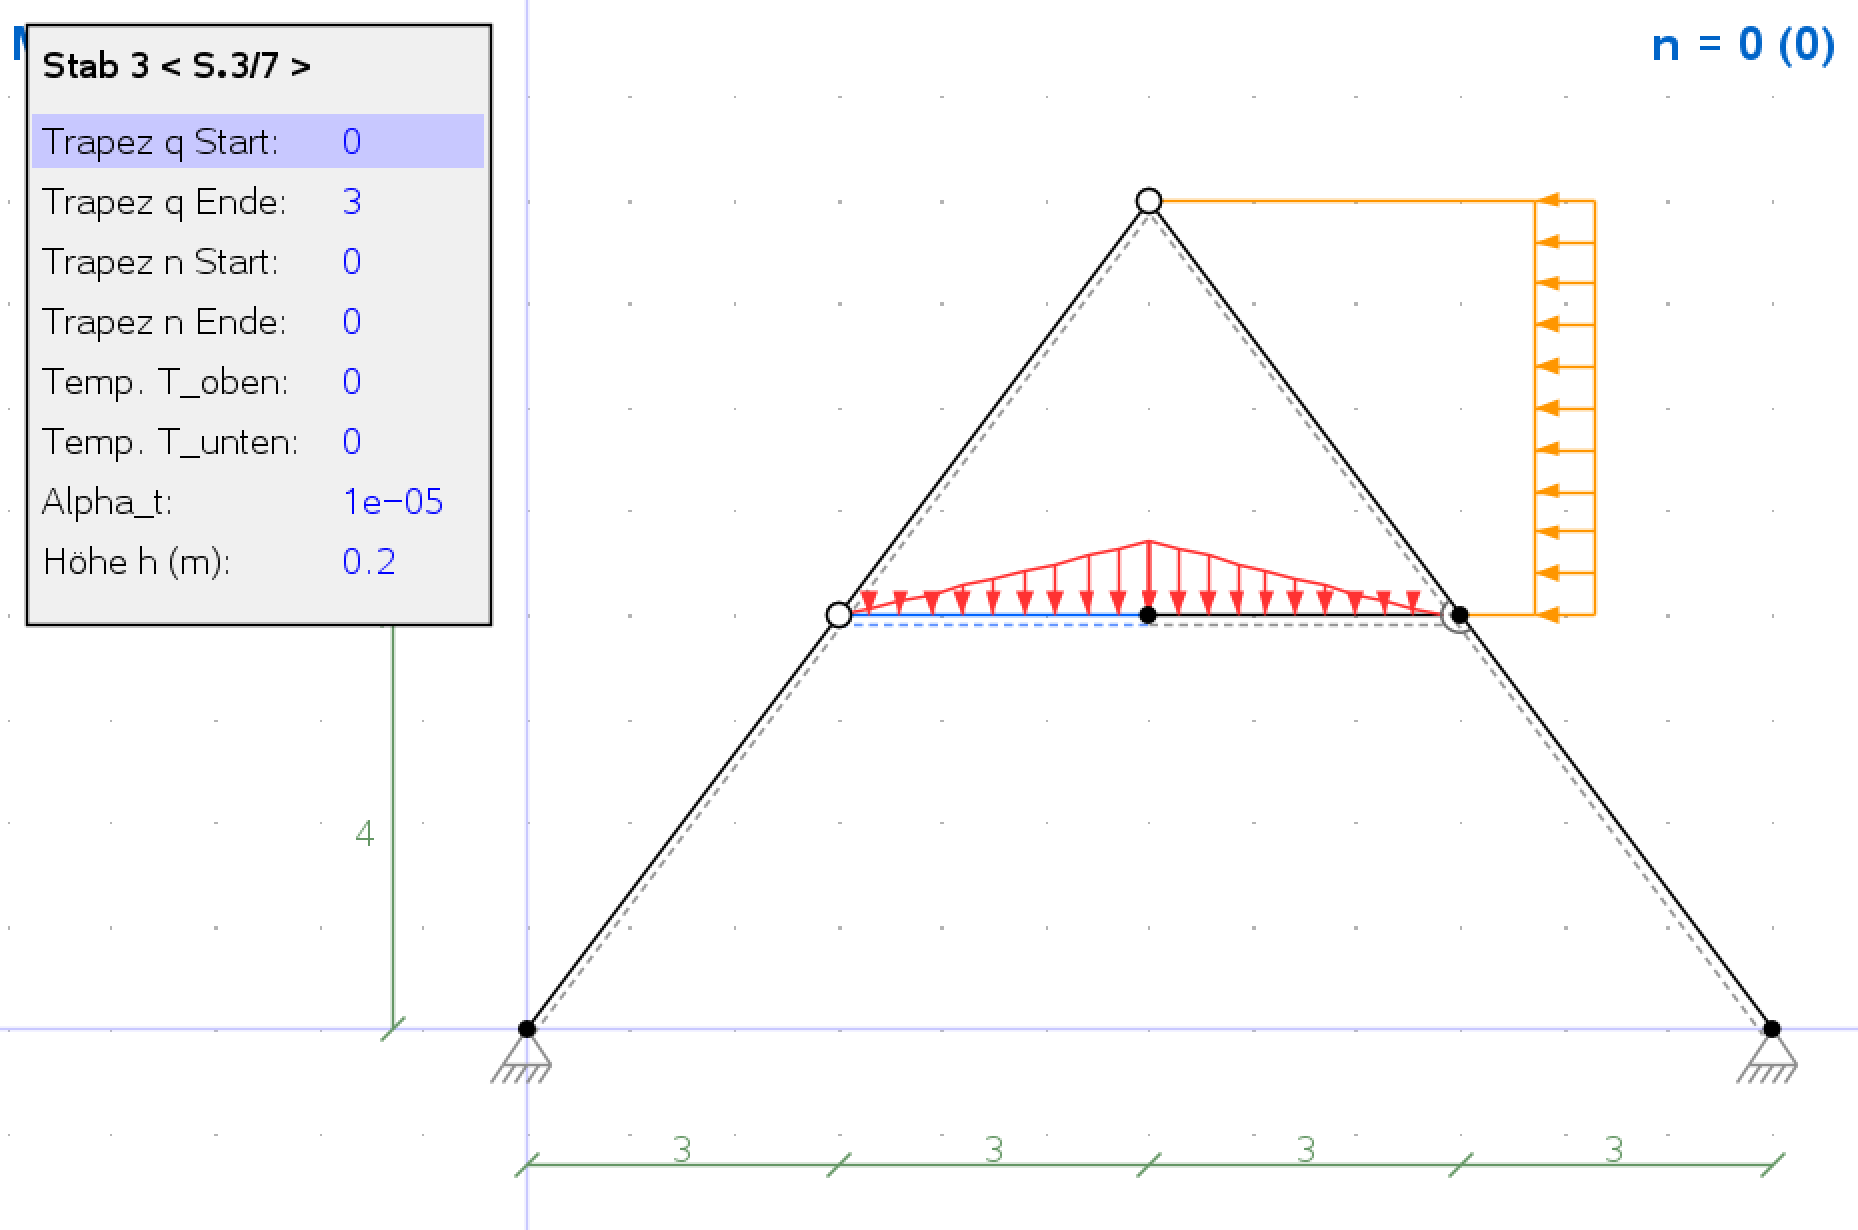
\includegraphics[width=\linewidth]{./fig/TM1/WiSe2122nr2_1.png}
        \caption{Trapezlast auf der linken Hälfte des Mittelstabs}
    \end{subfigure}
    \hfill
    \begin{subfigure}[t]{0.48\textwidth}
        \centering
        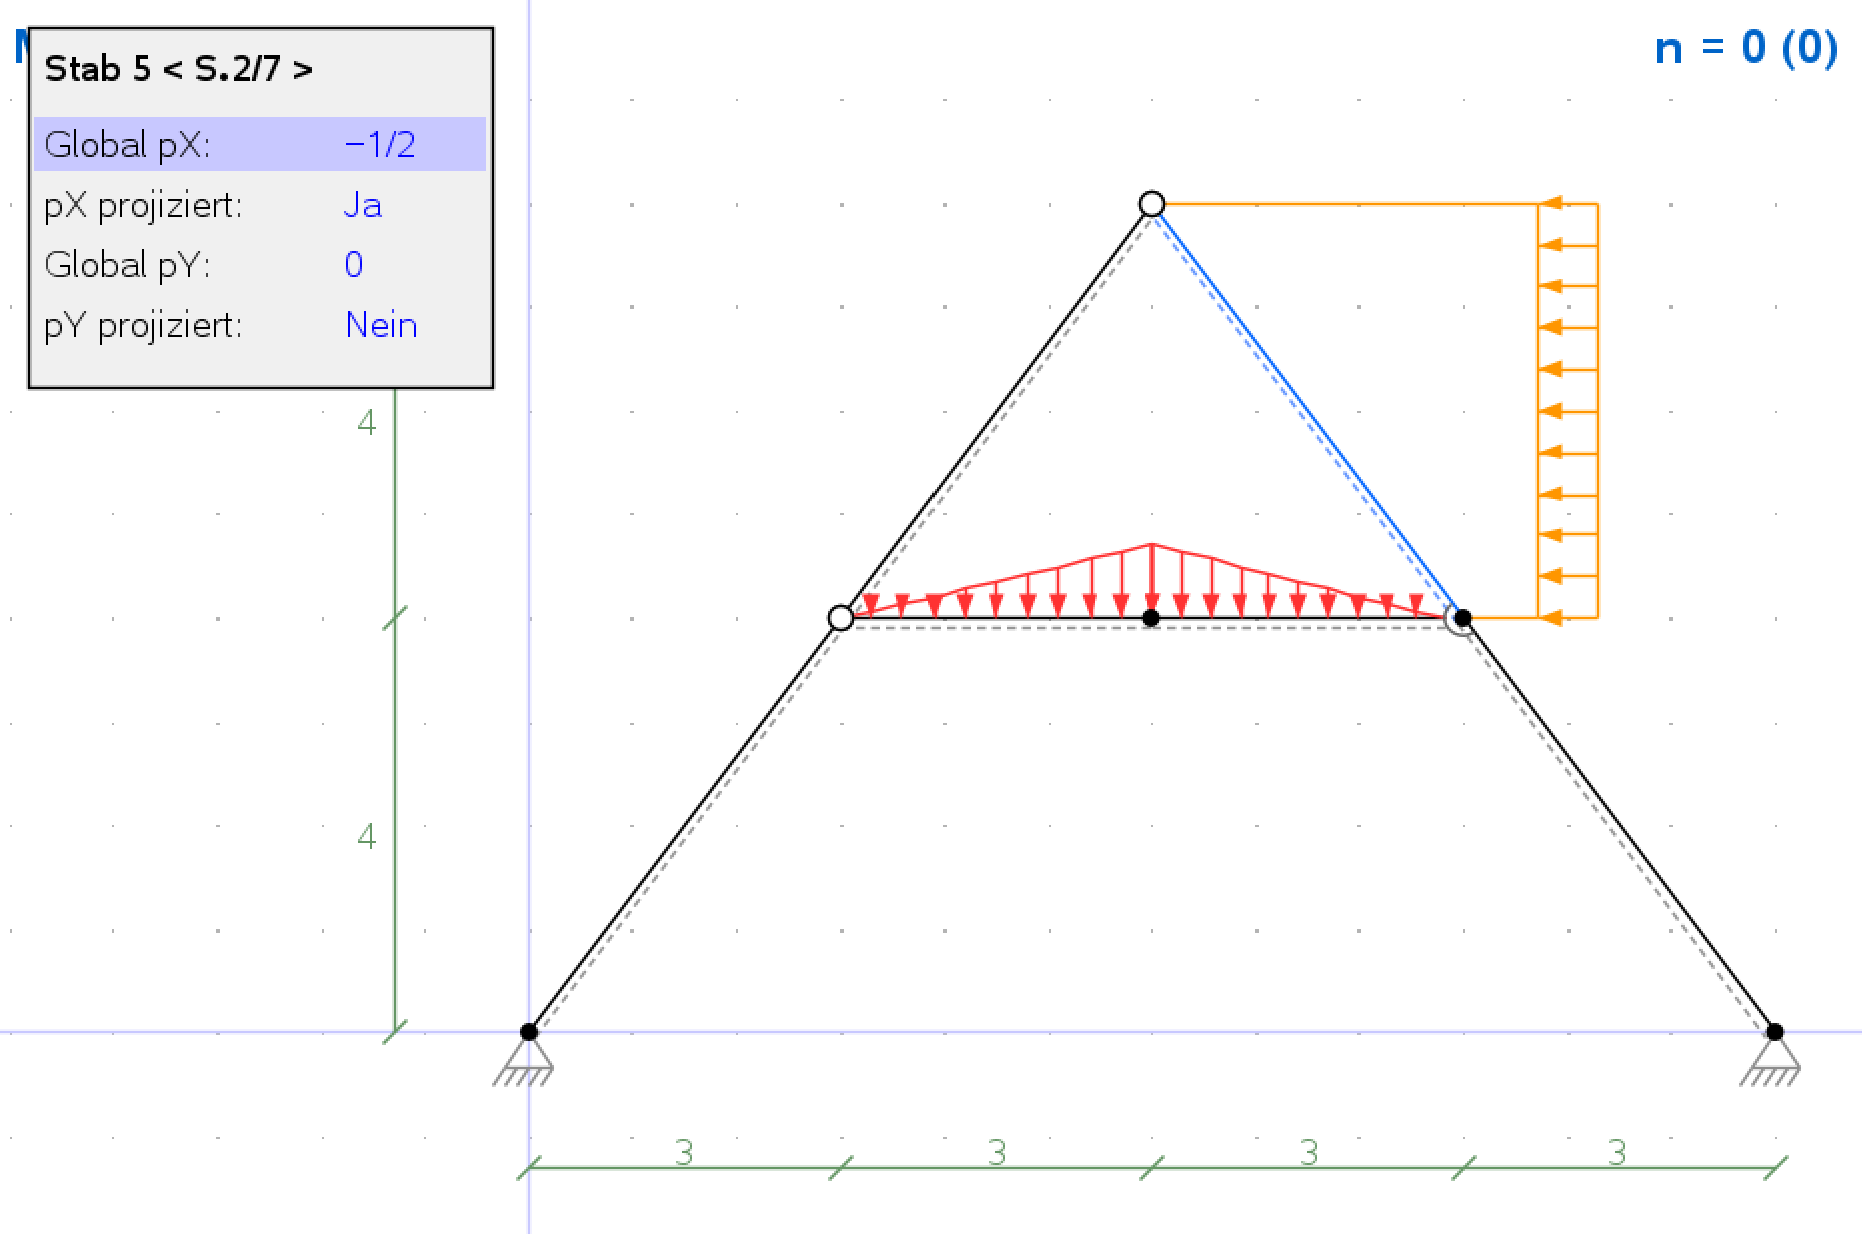
\includegraphics[width=\linewidth]{./fig/TM1/WiSe2122nr2_2.png}
        \caption{globale Streckenlast am oberen rechten Stab}
    \end{subfigure}
    \caption{WiSe~21/22, Nr.~2 im Programm}
    \label{fig:WiSe2122nr2_1}
\end{figure}

Den Stab in der Mitte müsst ihr im Programm teilen. Die Last auf ihm ist dreieckförmig mit der
Spitze in der Mitte, eine Trapezlast geht aber immer über einen ganzen Stab. Jede Hälfte bekommt
deshalb ihre eigene Trapezlast, die linke von $0$ auf $3$, die rechte von $3$ auf $0$
(Abb.~\ref{fig:WiSe2122nr2_1}a). Der neue Knoten in der Mitte bleibt biegesteif.

Die Streckenlast am schrägen Stab gebt ihr am einfachsten als globale Last ein
(Abb.~\ref{fig:WiSe2122nr2_1}b). In der Aufgabe ist sie auf die senkrechte Projektion des Stabes
bezogen, deshalb muss \emph{pX projiziert} auf \emph{Ja} stehen. Negativ ist sie, weil sie global
gesehen entgegen der $x$-Achse wirkt, also nach links.

Nach dem Berechnen könnt ihr das LGS, das zur Explosionsansicht (Abb.~\ref{fig:WiSe2122nr2_2})
gehört, über die zweite Seite des Obermenüs (\emph{LGS-Matrix}) in den Taschenrechner exportieren
(Abb.~\ref{fig:WiSe2122nr2_3}). Die Gleichungen stehen dann lesbar in \code{lgs}, die Lösung
bekommt ihr zum Beispiel mit \code{ggw\_x = ggw\_a$^{-1}$*ggw\_b}
(Abschnitt~\ref{sec:lgs-matrix}).

\begin{figure}[htbp]
    \centering
    \begin{subfigure}[t]{0.48\textwidth}
        \centering
        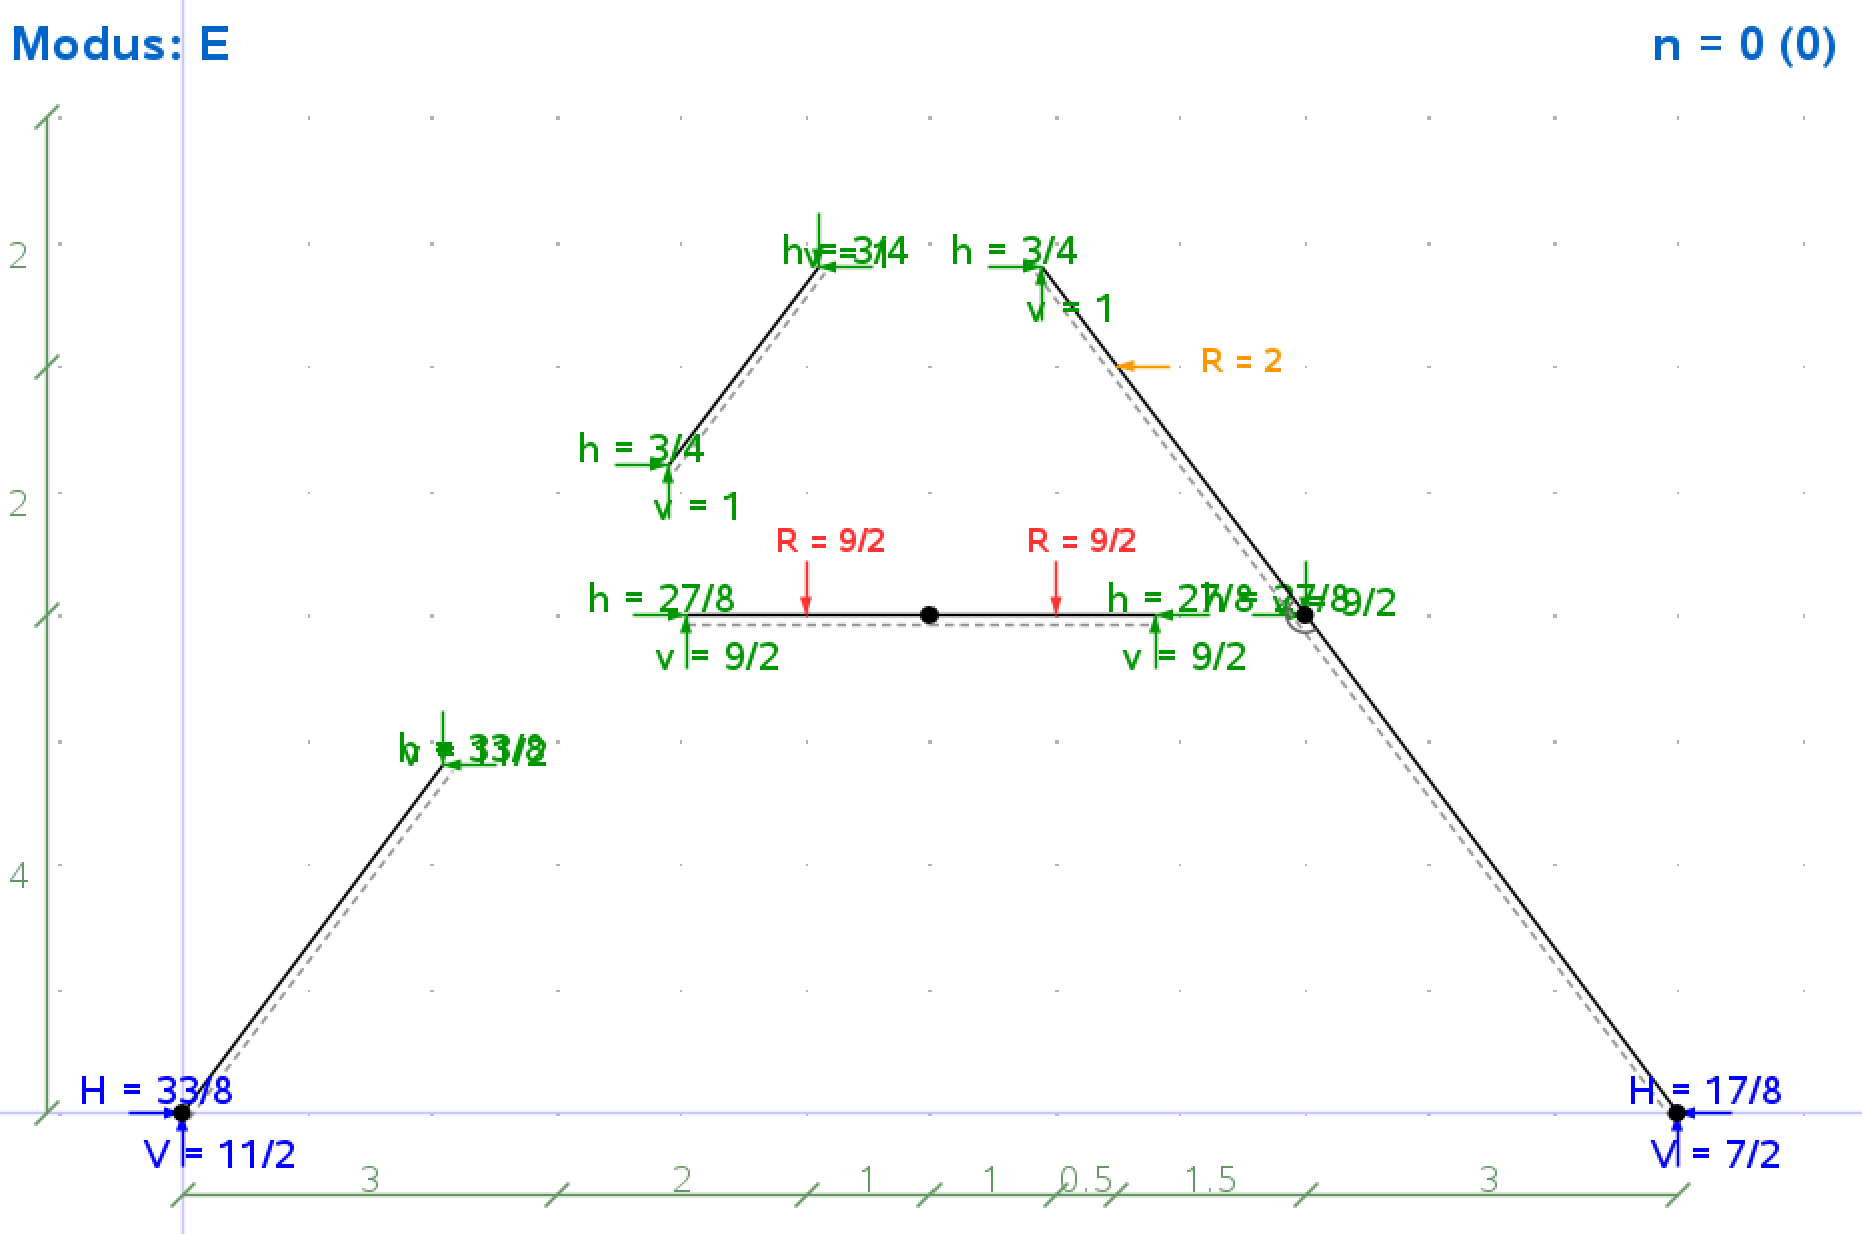
\includegraphics[width=\linewidth]{./fig/TM1/WiSe2122nr2_5.png}
        \caption{Seite~1: Ergebnisse in ihrer wirklichen Richtung}
    \end{subfigure}
    \hfill
    \begin{subfigure}[t]{0.48\textwidth}
        \centering
        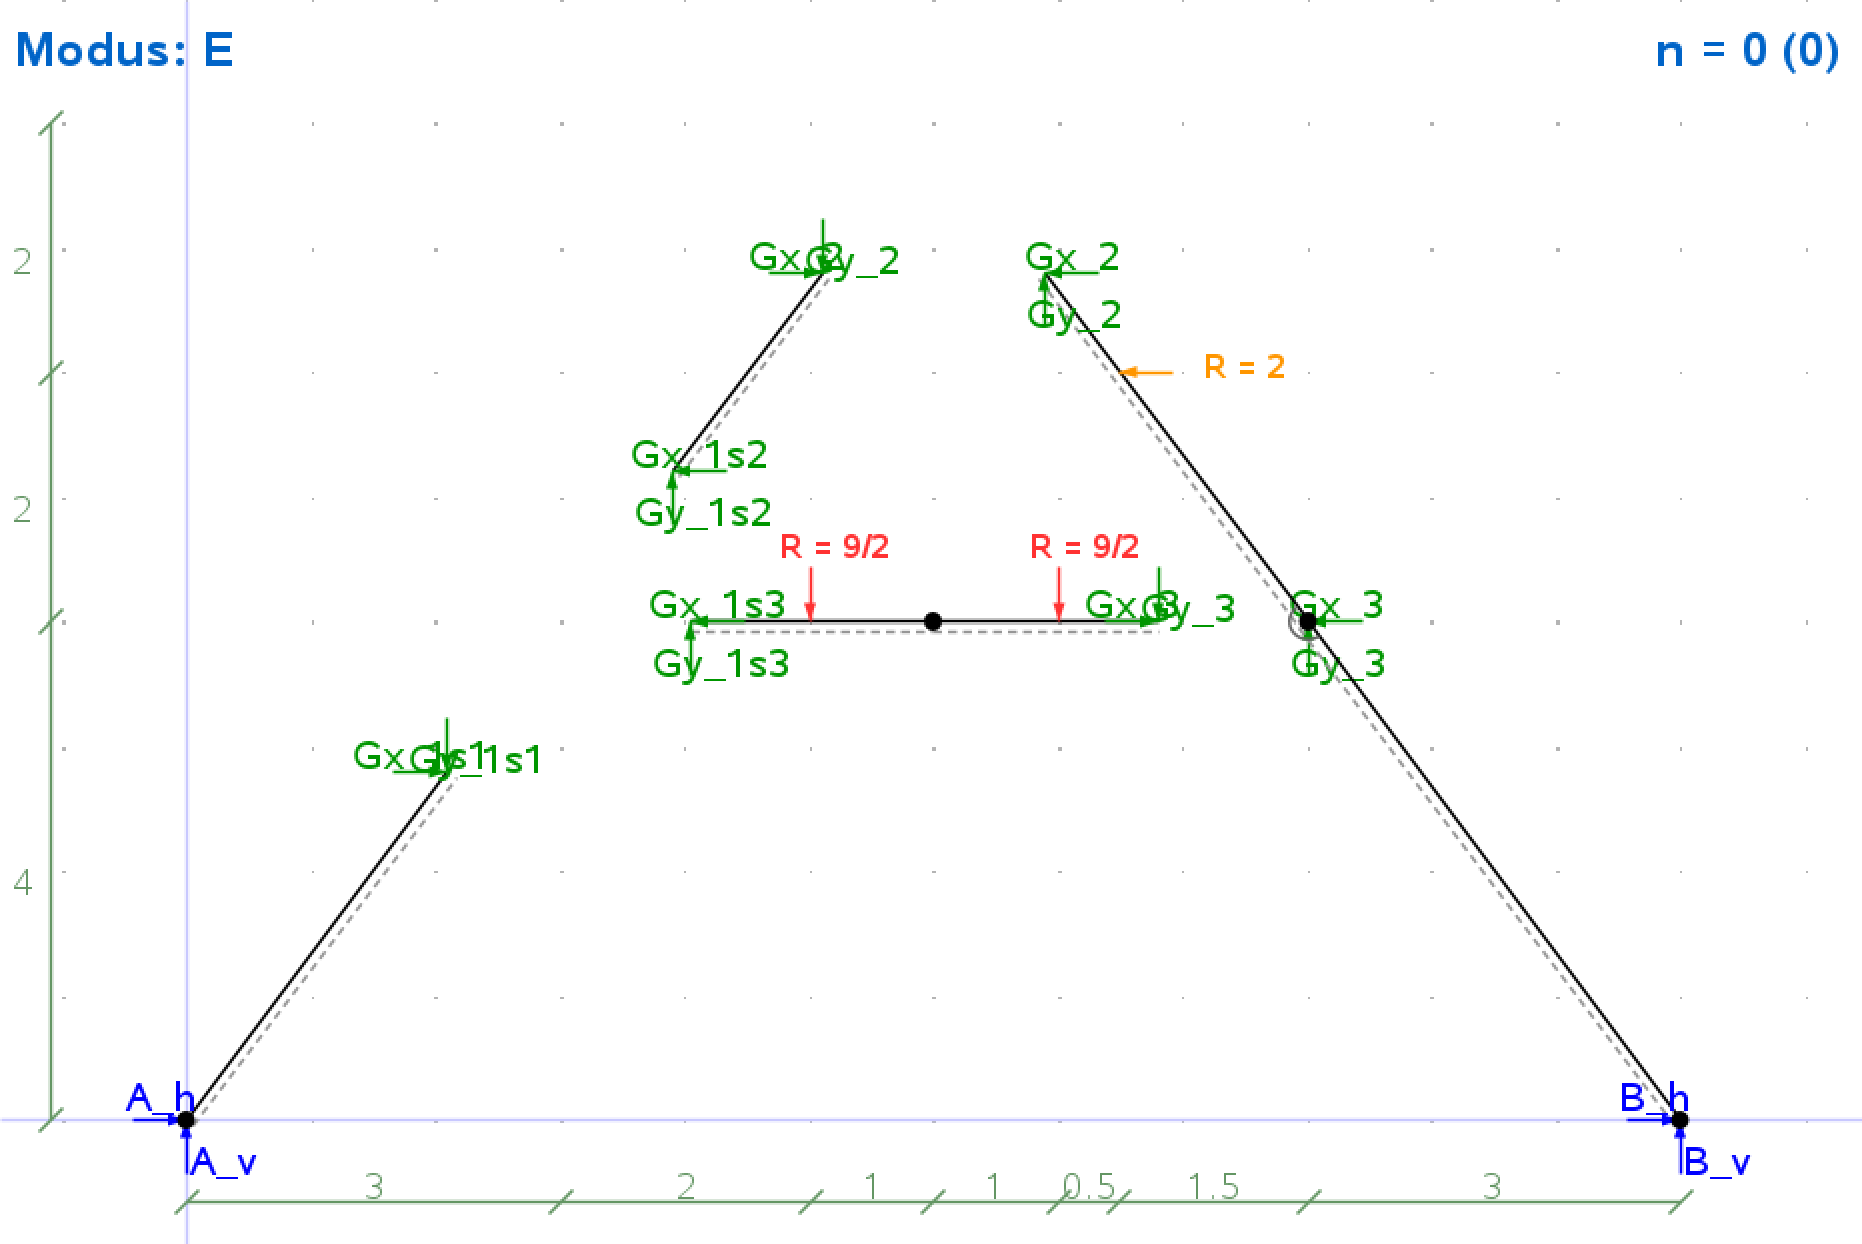
\includegraphics[width=\linewidth]{./fig/TM1/WiSe2122nr2_6.png}
        \caption{Seite~2: Unbekannte in positiver Richtung}
    \end{subfigure}
    \caption{WiSe~21/22, Nr.~2: Explosionsansicht (E-Modus)}
    \label{fig:WiSe2122nr2_2}
\end{figure}

\begin{figure}[htbp]
    \centering
    \begin{subfigure}[t]{0.48\textwidth}
        \centering
        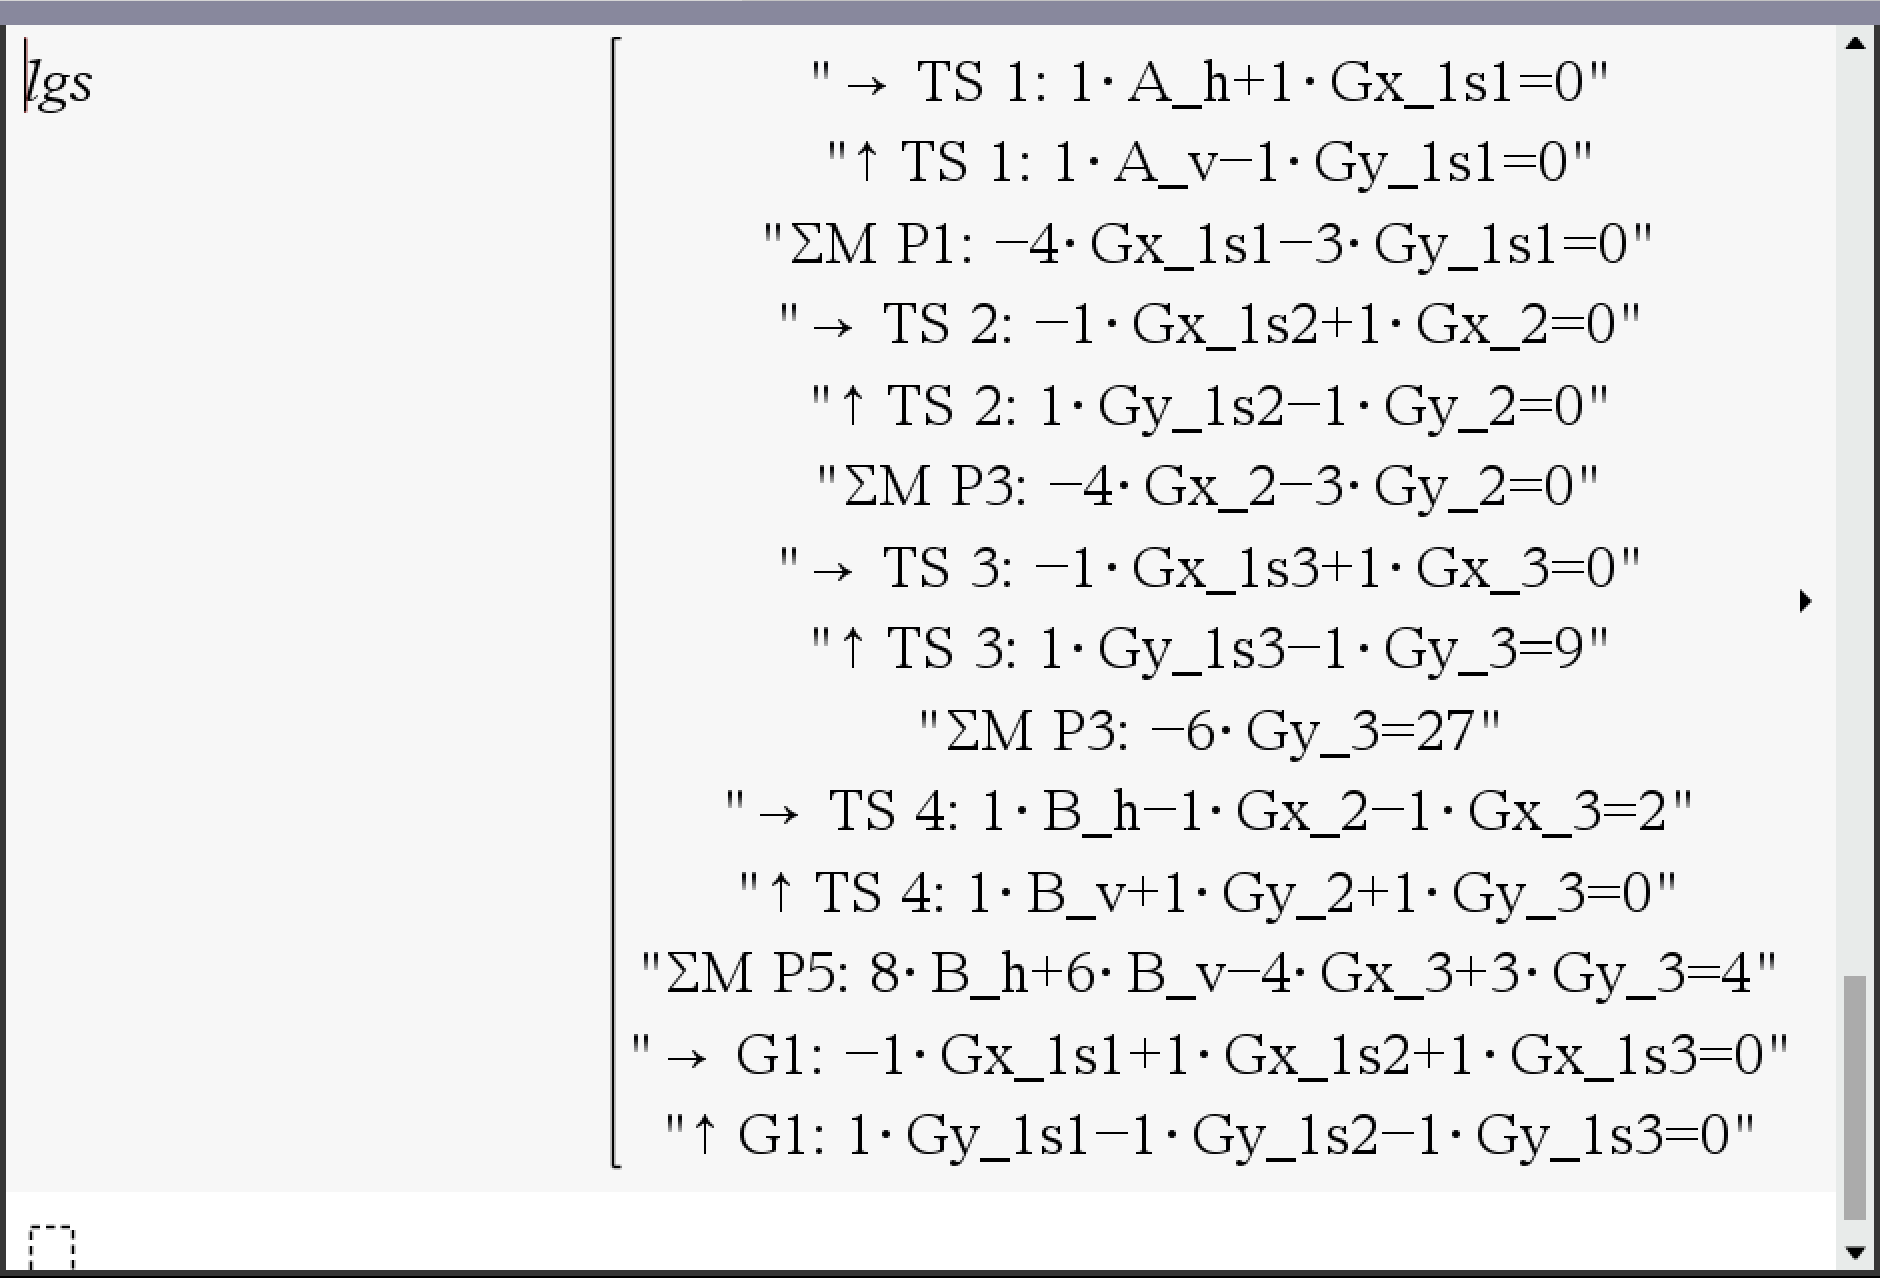
\includegraphics[width=\linewidth]{./fig/TM1/WiSe2122nr2_3.png}
        \caption{exportierte Gleichungen \code{lgs}}
    \end{subfigure}
    \hfill
    \begin{subfigure}[t]{0.48\textwidth}
        \centering
        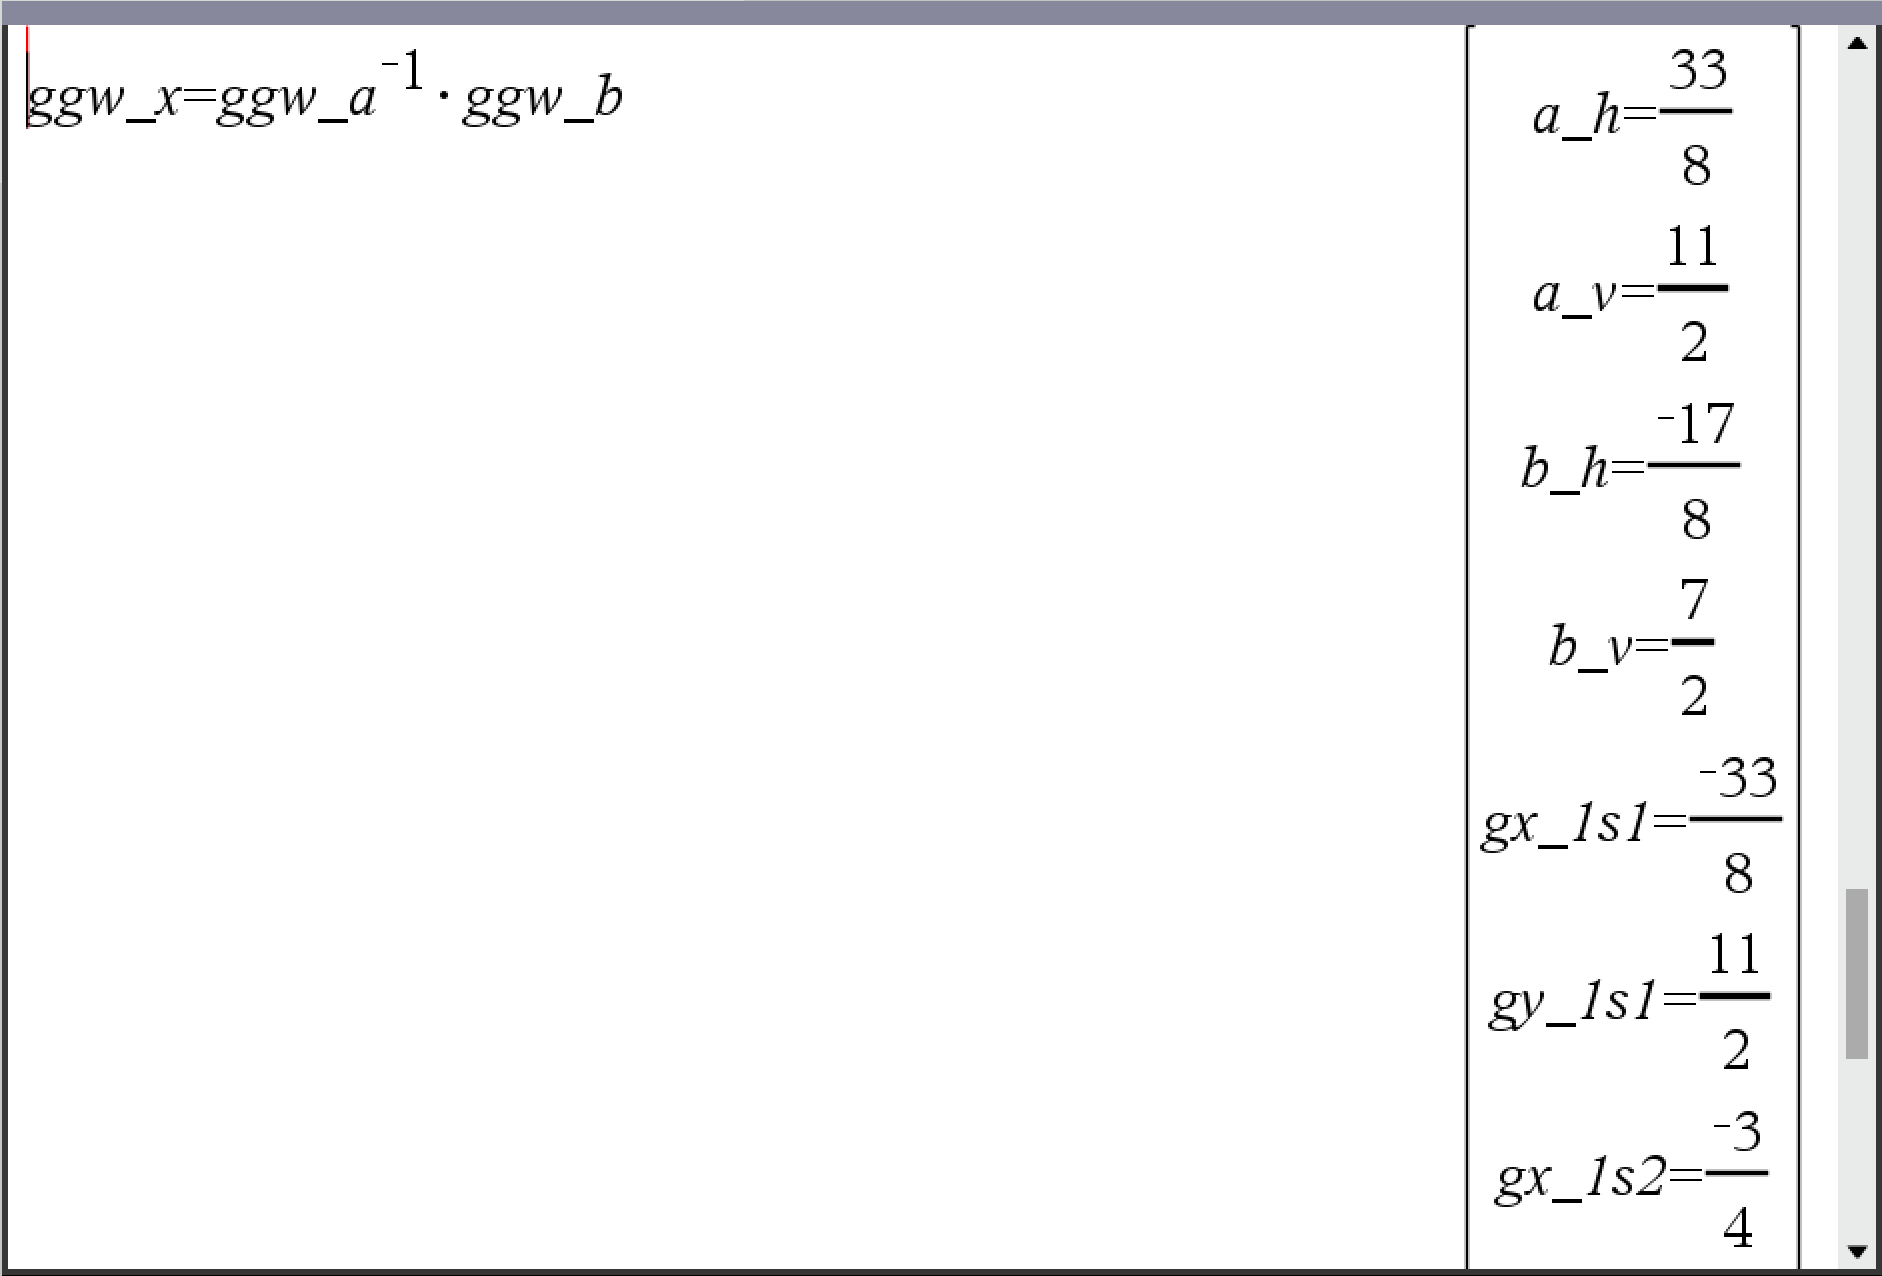
\includegraphics[width=\linewidth]{./fig/TM1/WiSe2122mr2_4.png}
        \caption{Lösung mit \code{ggw\_x}}
    \end{subfigure}
    \caption{WiSe~21/22, Nr.~2: exportiertes LGS}
    \label{fig:WiSe2122nr2_3}
\end{figure}

Die Explosionsansicht kann manchmal etwas unübersichtlich sein. Wenn ihr nah genug heranzoomt,
sollte aber trotzdem alles erkennbar sein. Die Ergebnisse müsst ihr natürlich nicht in dieser
Vektorform aufschreiben, nur ihr Inhalt zählt.

An dieser Stelle will ich anmerken, dass meist nur bei Systemen mit einem geschlossenen Ring wie
diesem nach allen Gelenk- und Auflagerkräften gefragt wird. Bei offenen Systemen ohne Ring wird oft
nur nach den Auflagerkräften gefragt. Das exportierte LGS liefert dann zwar auch die richtige Lösung, ist aber
meist mehr, als ihr braucht. Den Punkt, um den das Programm die Momentensumme eines Teilsystems
bildet, seht ihr, wenn ihr in der Explosionsansicht mit der Maus über das Teilsystem fahrt
(\emph{Hover}).

Die Zustandslinien, also die Verläufe der Schnittgrößen, zeichnet euch das Programm mit den Tasten
\taste{n}, \taste{q} und \taste{m}, die könnt ihr einfach abzeichnen. Falls ihr Randwerte schlecht
erkennt, fahrt mit der Maus über den jeweiligen Stab, dann zeigt das Programm nur noch diesen Stab
mit seinen Randwerten an.

\subsubsection{Qualitavtive Verläufe im symbolischen Modus (Nr.~4)}

Um meinen den oben genannten Punkt zum symbolischen Modus zu verdeutlichen will ich hier kurz auf Teilaufgabe b) eingehen.
Das System und der Querkraftverlauf sind in Abbildung~\ref{fig:TM1WiSe2122Nr4} dargestellt.

\begin{figure}[htbp]
    \centering
    \begin{subfigure}[t]{0.48\textwidth}
        \centering
        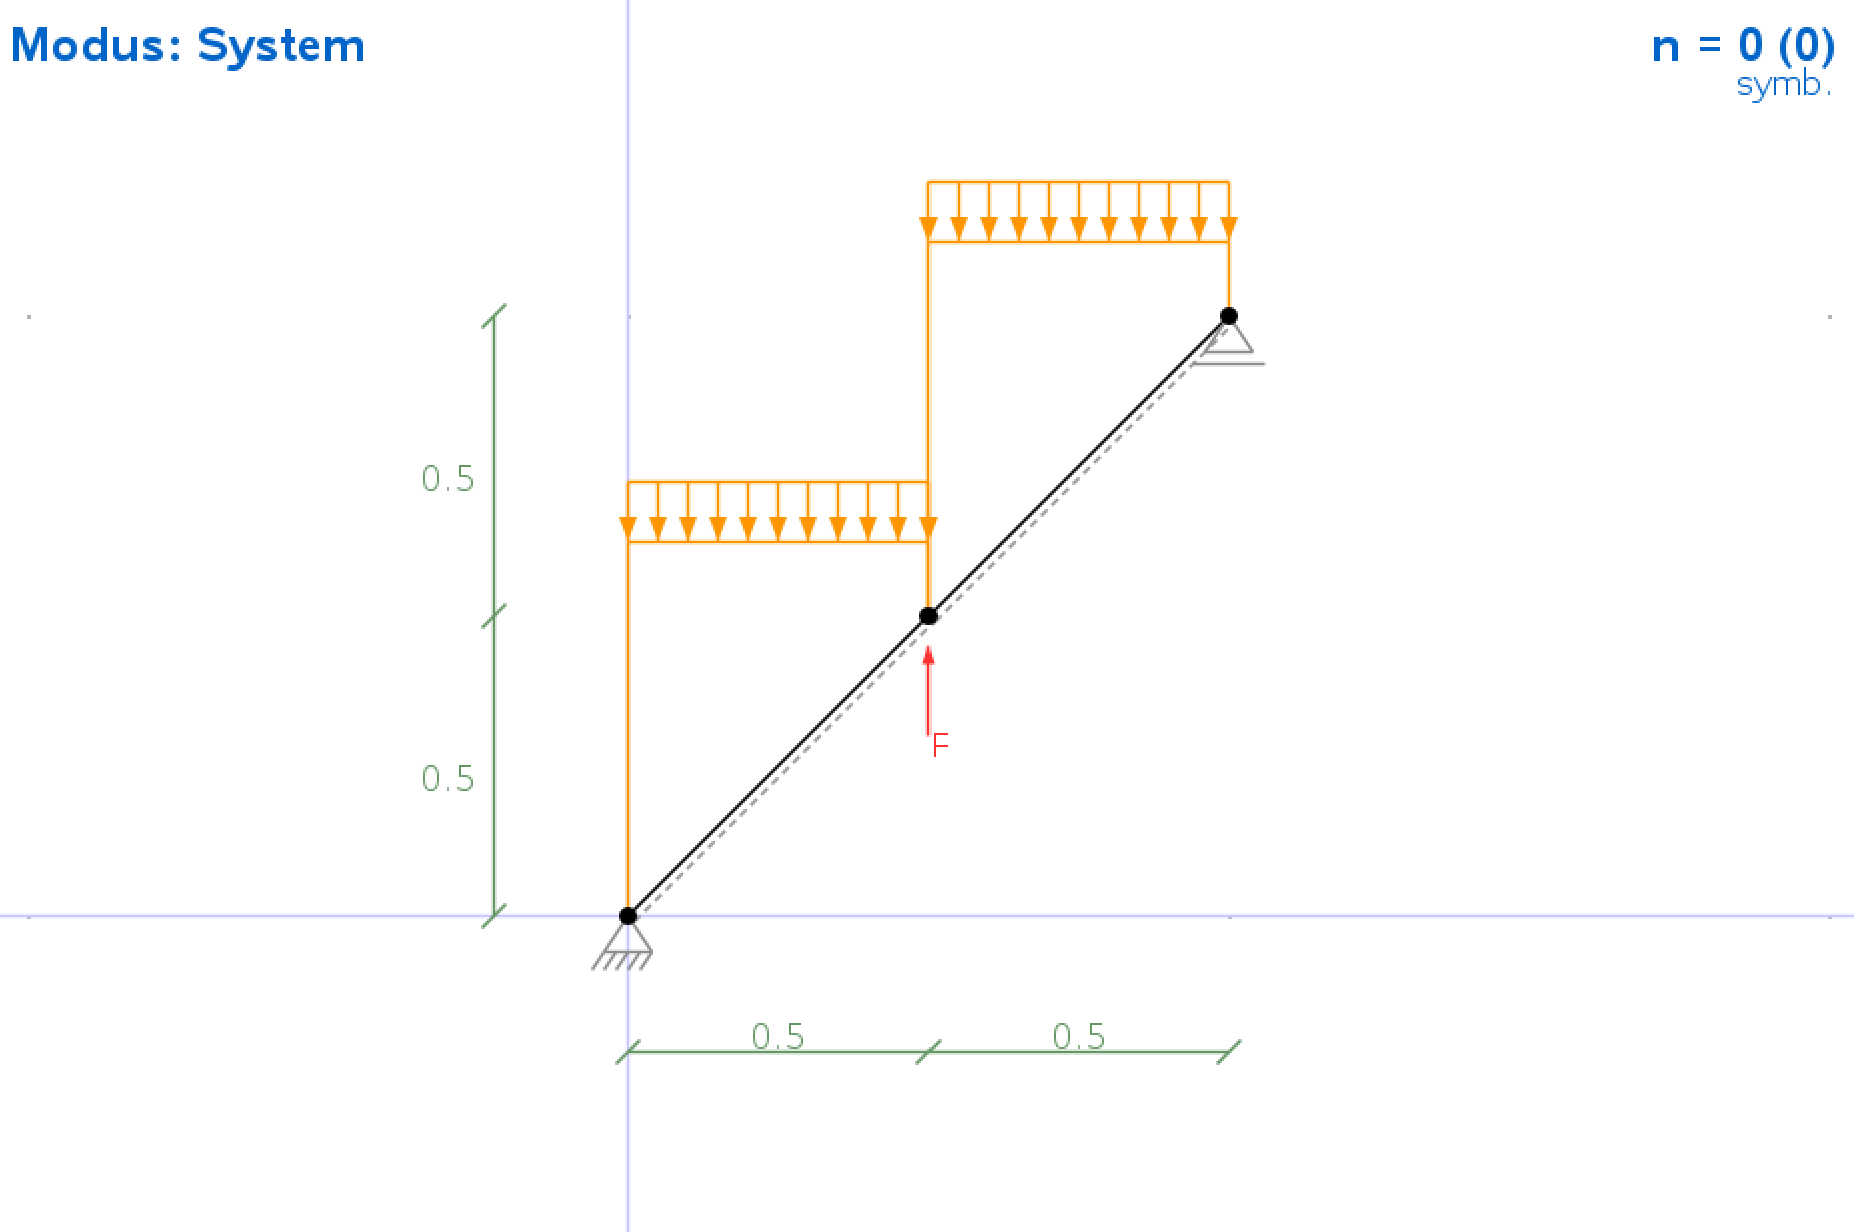
\includegraphics[width=\linewidth]{./fig/TM1/WiSe2122nr4_1.png}
        \caption{System}
    \end{subfigure}
    \hfill
    \begin{subfigure}[t]{0.48\textwidth}
        \centering
        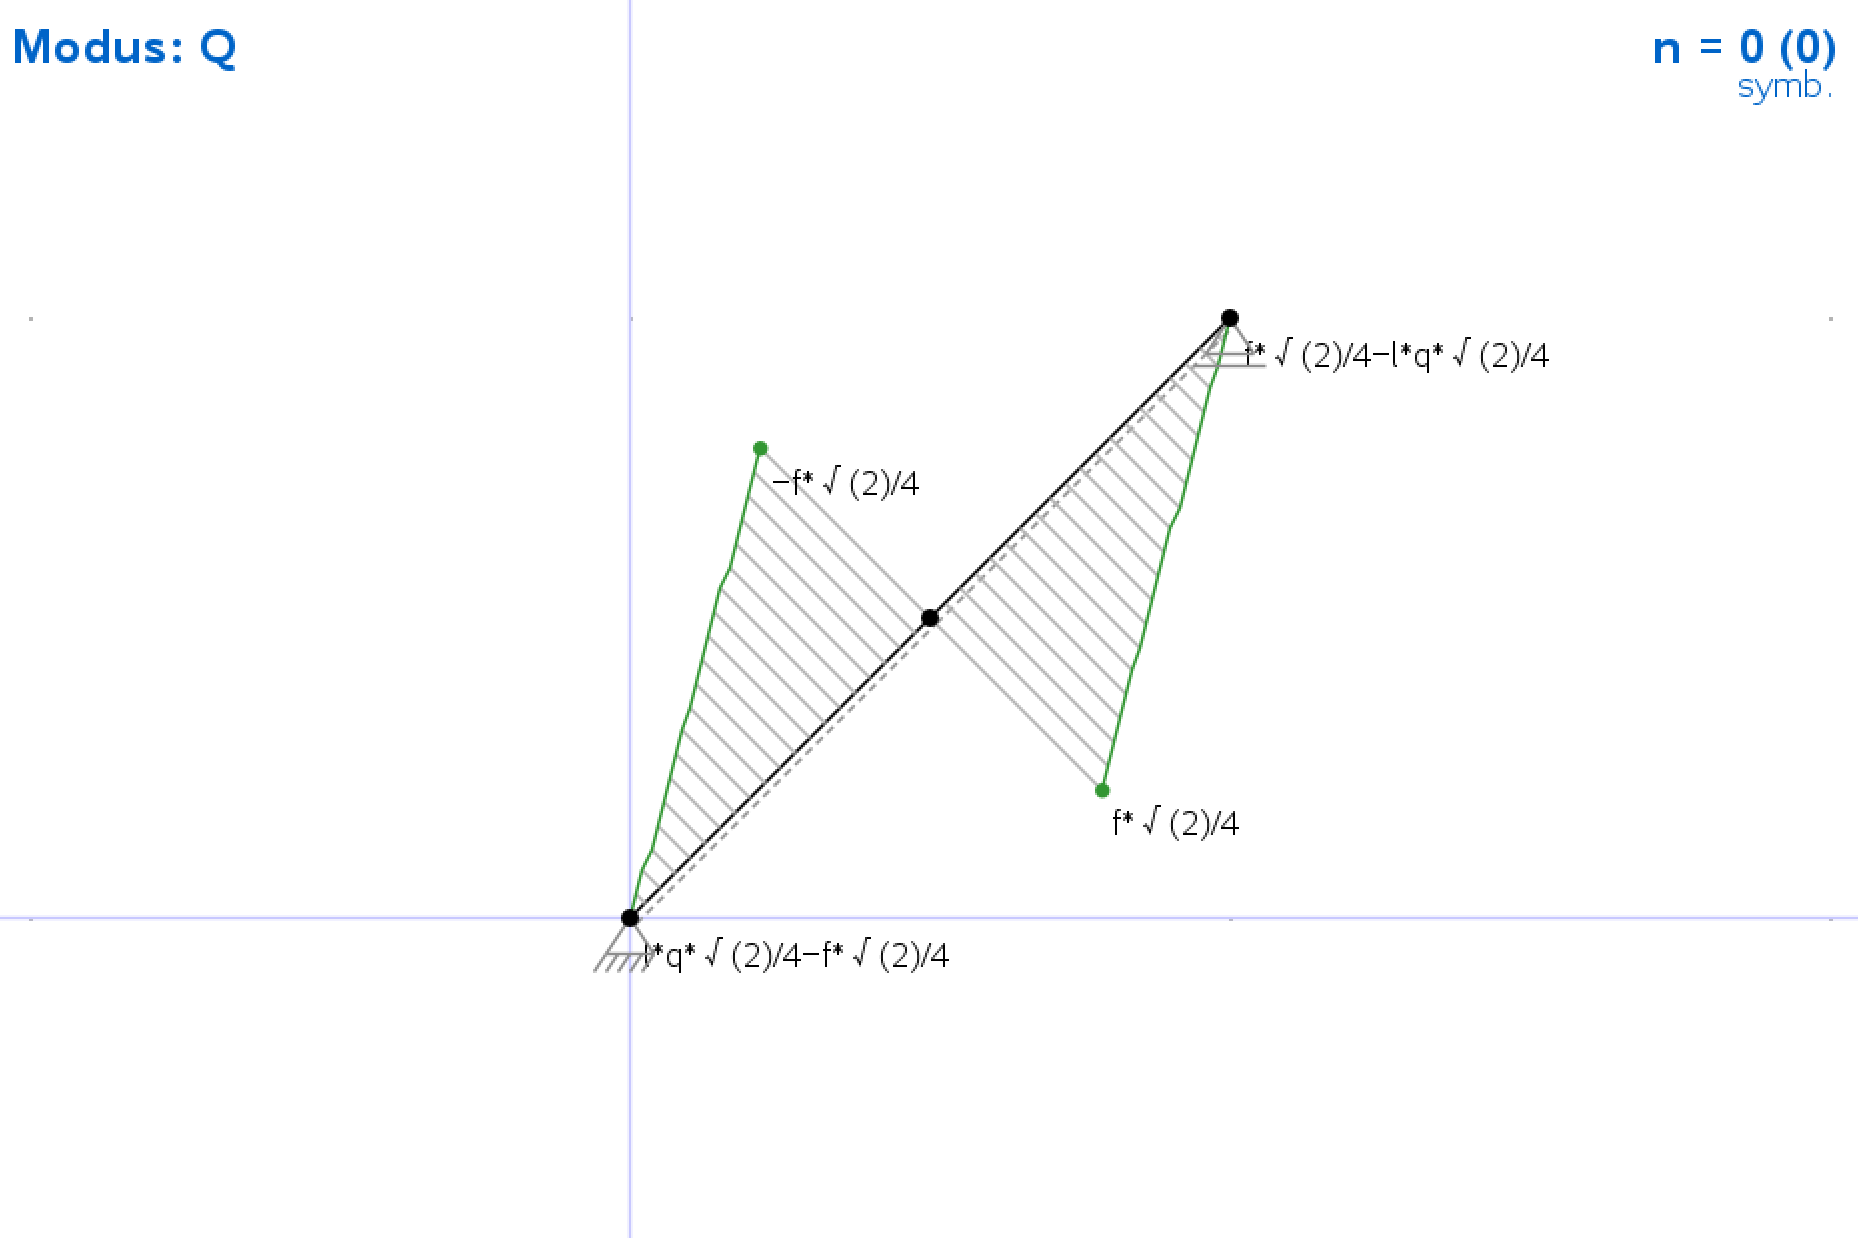
\includegraphics[width=\linewidth]{./fig/TM1/WiSe2122nr4_2.png}
        \caption{Querkraftverlauf}
    \end{subfigure}
    \caption{WiSe~21/22, Nr.~4}
    \label{fig:TM1WiSe2122Nr4}
\end{figure}

Im Querkraft verlauf sieht es so aus, als ob diese an den Auflagern null wird. Wenn man sich die Beschriftung der Randwerte 
anschaut wird jedoch klar, dass ist nur der Fall, wenn $q\cdot l=F$ bzw. $q\cdot a=F$ gilt. Das ist eben genau die Annhame des Programms,
um überhaupt irgendeinen Verlauf zeichnen zu können.
Die Aufgabe gibt aber unten vor: $F>q\cdot a$. Damit wird die Qerkraft am linekn Ende negativ und am rechten Ende positiv.
Die Verläufe von symbolische Berechnungen solltet ihr also \textbf{nie} einfach blind abzeichnen.

\subsection{PvV (Nr.~3)}

Zum PvV gibt es eigentlich nicht viel zu sagen. System zeichnen, \taste{v} drücken, Bindung wählen, abzeichnen,
dann exportieren und aufschreiben. 


\begin{figure}[htbp]
    \centering
    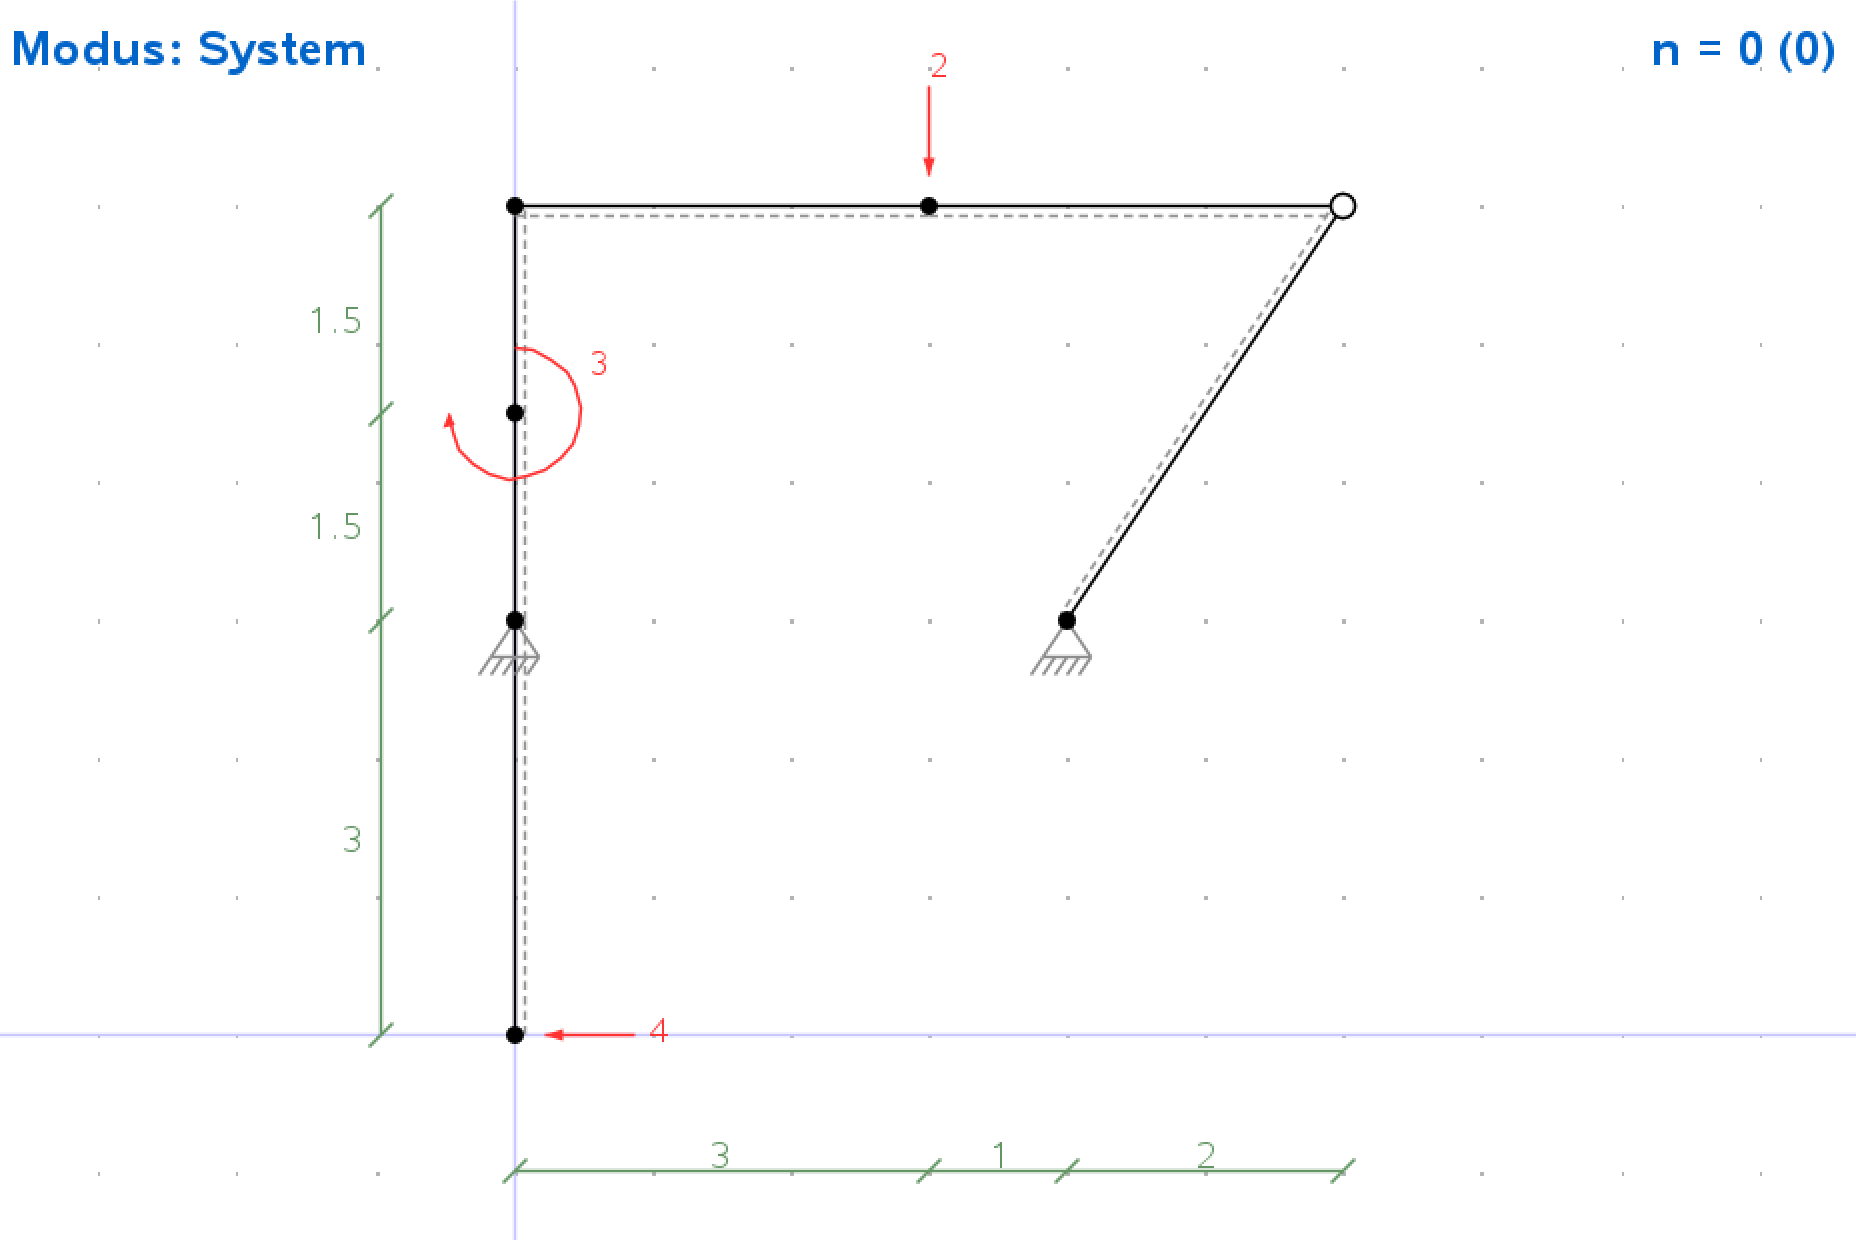
\includegraphics[width=0.5\linewidth]{./fig/TM1/WiSe2122nr3_1.png}
    \caption{TM1 WiSe~21/22, Nr.~3 im Programm}
    \label{fig:TM1WiSe2122Nr3_1}
\end{figure}

\begin{figure}[htbp]
    \centering
    \begin{subfigure}[t]{0.48\textwidth}
        \centering
        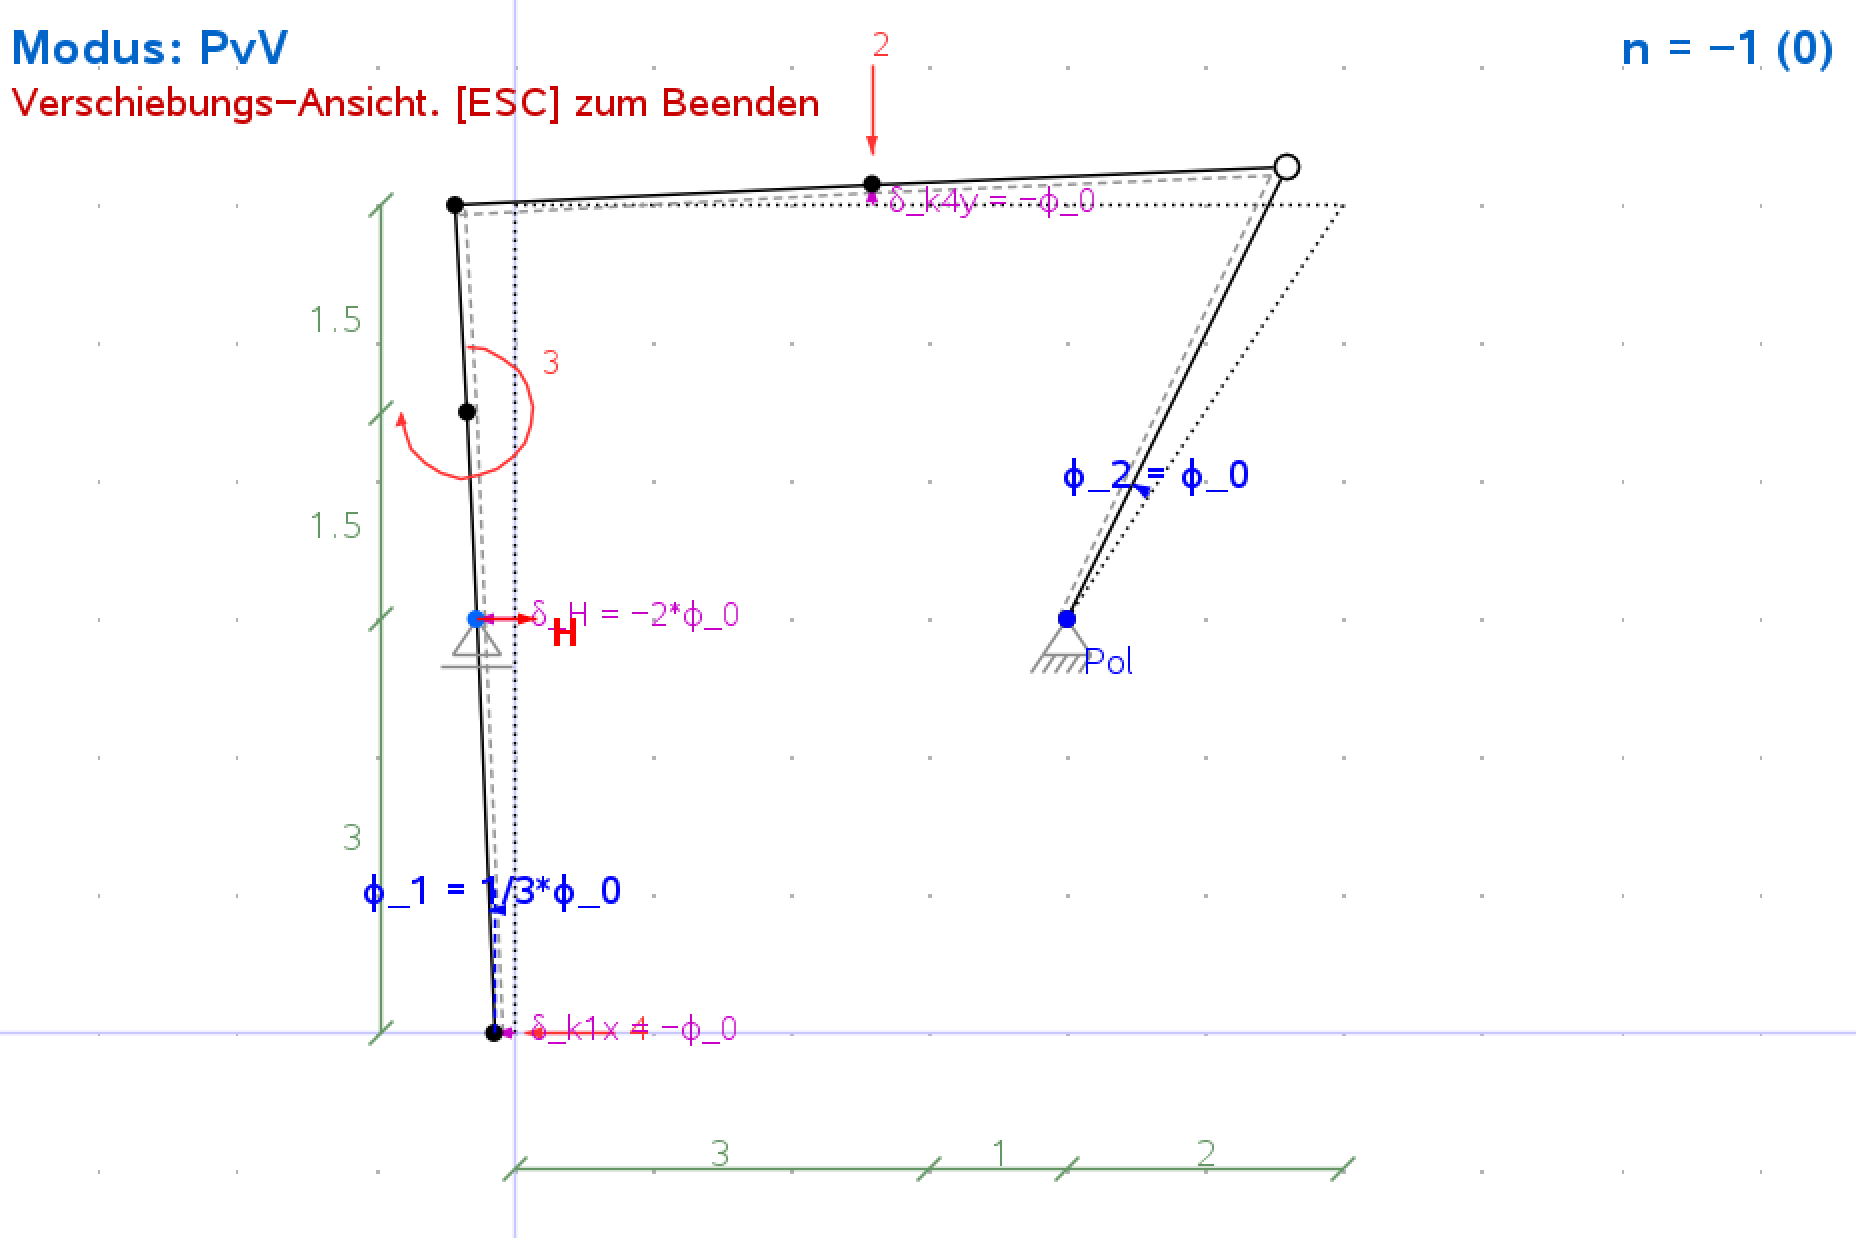
\includegraphics[width=\linewidth]{./fig/TM1/WiSe2122nr3_2.png}
        \caption{Verschiebungsfigur für $A_H$}
    \end{subfigure}
    \hfill
    \begin{subfigure}[t]{0.48\textwidth}
        \centering
        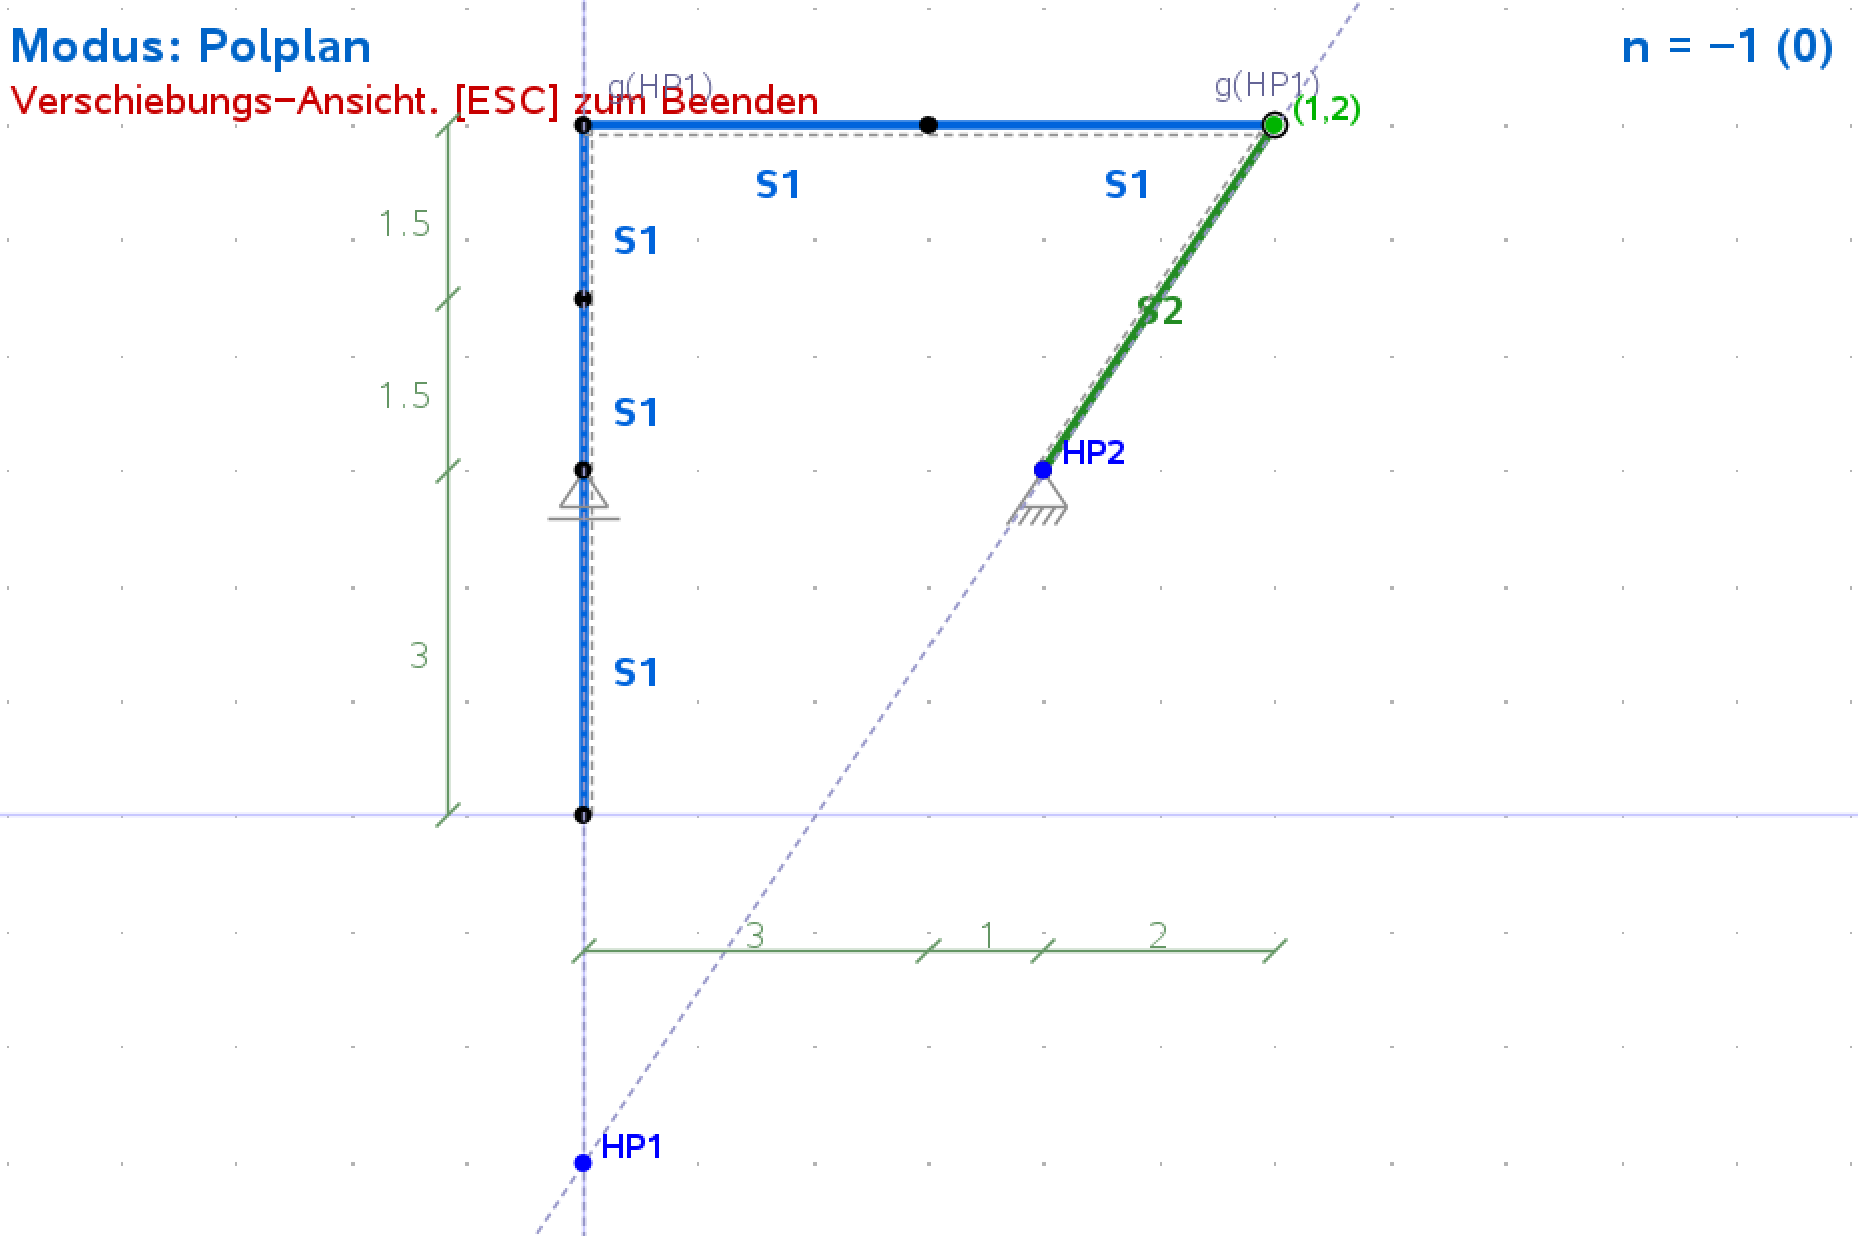
\includegraphics[width=\linewidth]{./fig/TM1/WiSe2122nr3_3.png}
        \caption{Polplan für $A_H$}
    \end{subfigure}
    \caption{WiSe~21/22, Nr.~3: $A_H$}
    \label{fig:TM1WiSe2122Nr3_2}
\end{figure}

\begin{figure}[htbp]
    \centering
    \begin{subfigure}[t]{0.48\textwidth}
        \centering
        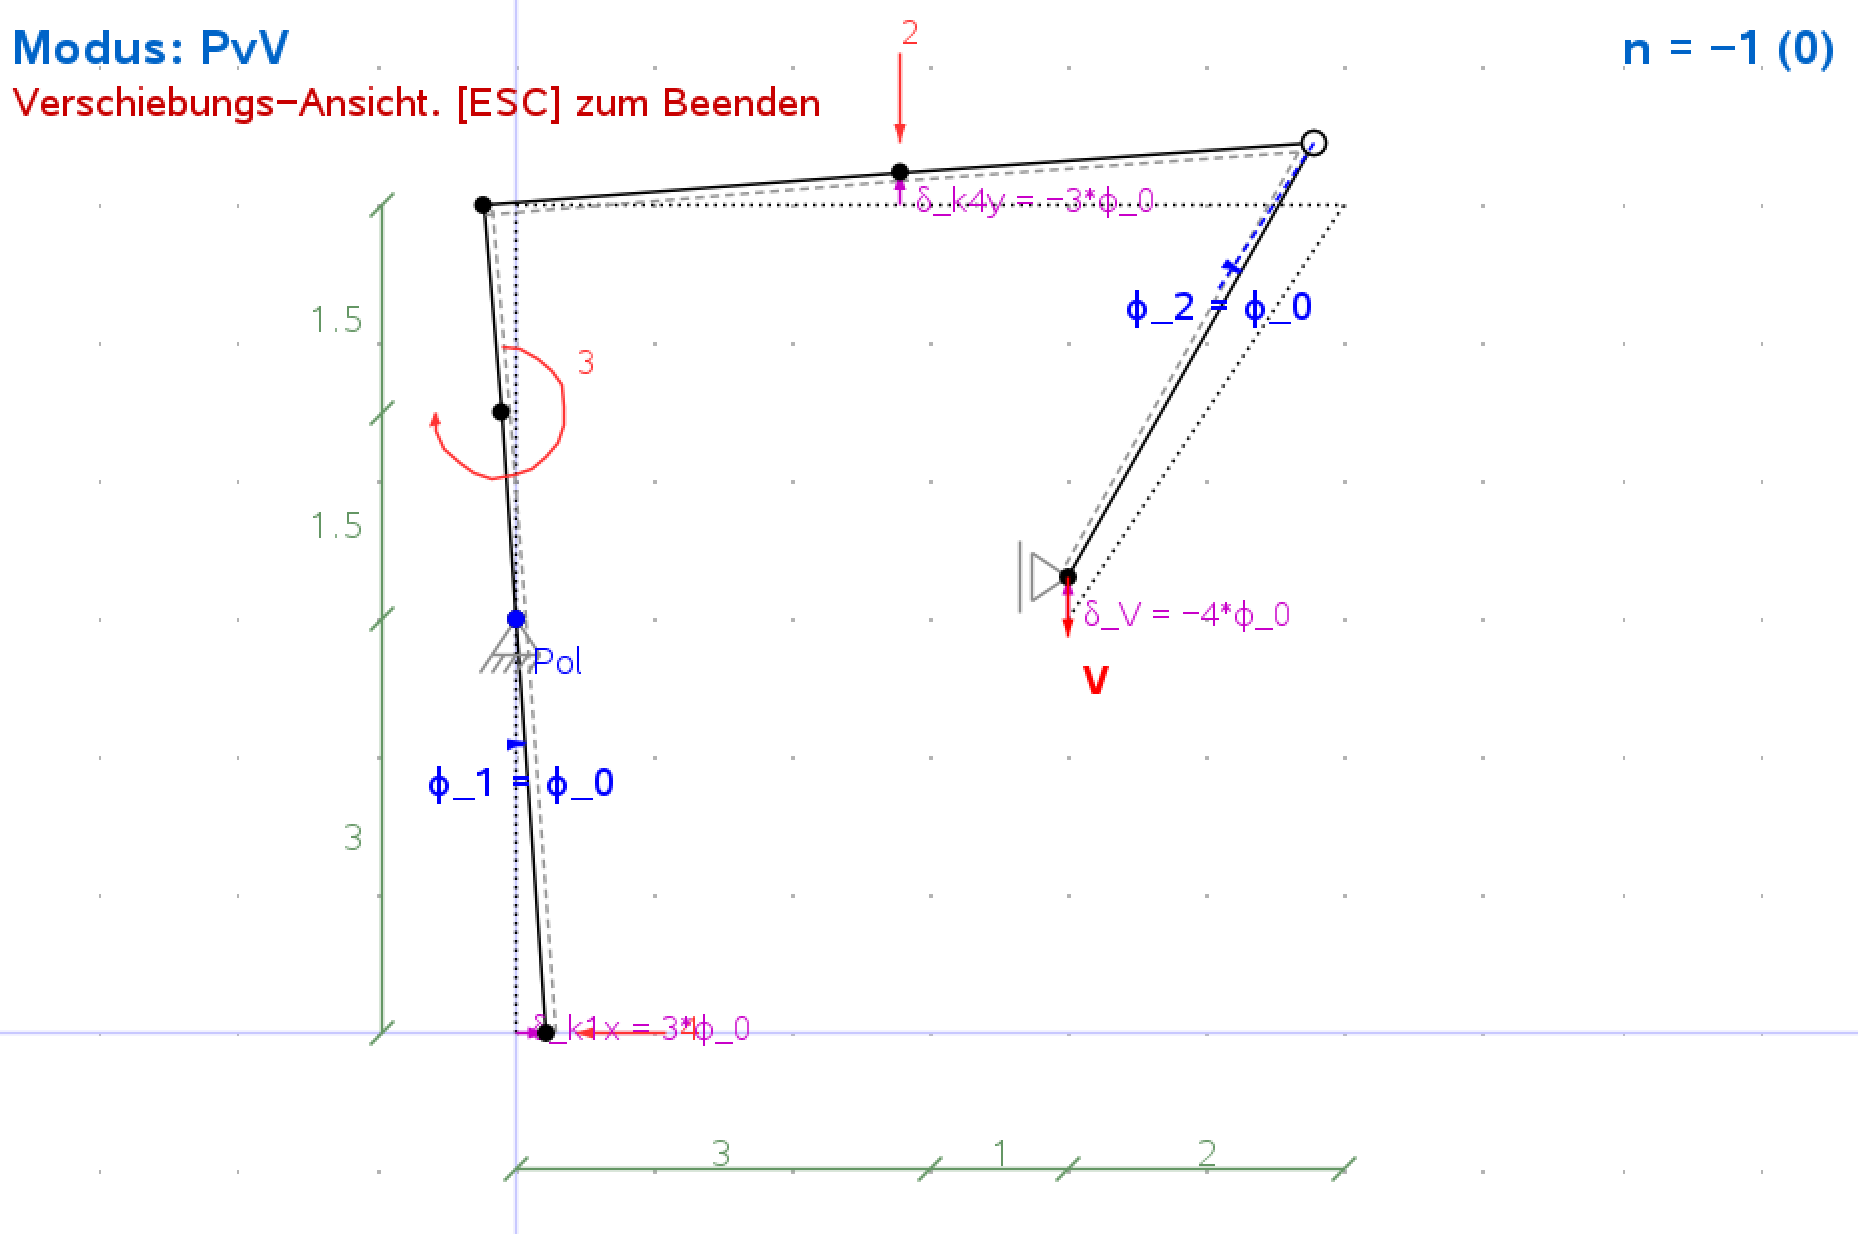
\includegraphics[width=\linewidth]{./fig/TM1/WiSe2122nr3_4.png}
        \caption{Verschiebungsfigur für $B_V$}
    \end{subfigure}
    \hfill
    \begin{subfigure}[t]{0.48\textwidth}
        \centering
        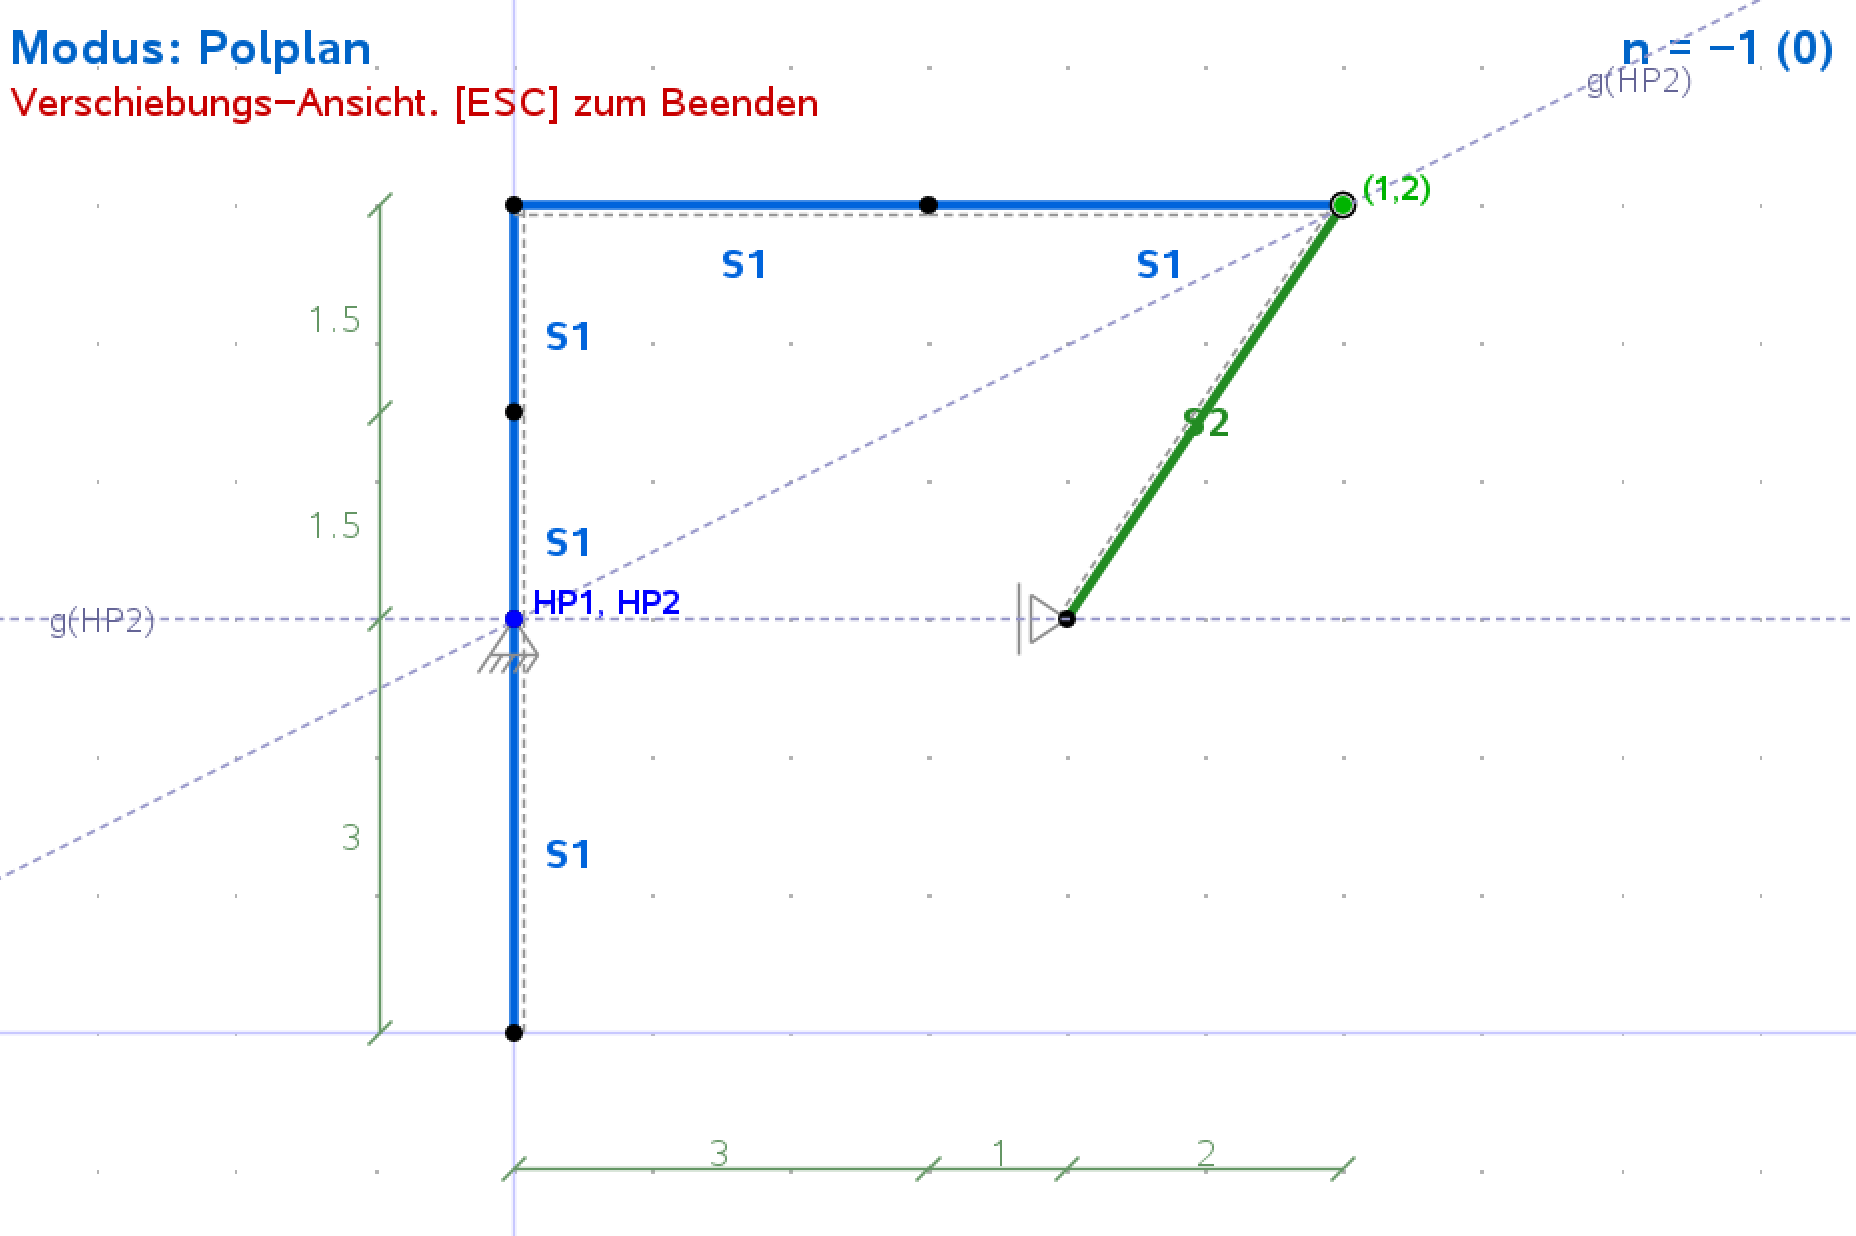
\includegraphics[width=\linewidth]{./fig/TM1/WiSe2122nr3_5.png}
        \caption{Polplan für $B_V$}
    \end{subfigure}
    \caption{WiSe~21/22, Nr.~3: $B_V$}
    \label{fig:TM1WiSe2122Nr3_3}
\end{figure}

Die Zeilen der Matrizen \code{pvv\_kin} und \code{pvv\_pol} (Abb.~\ref{fig:TM1WiSe2122Nr3_4})
sind als Gleichungskette zu lesen. Hier gilt also z.B. $\delta_{k1x}= -3\cdot\varphi_1=-\varphi_0$, oder 
$\delta x_{p12}= -9\cdot\varphi_1=-3\varphi_2$. Mit diesen Gleichungen lässt sich aus \code{w\_eq1} \code{w\_eq2} bauen.
Diese gleichung lässt sich dann entweder von hand oder mit dem Taschenrechner nach der gesuchten Größe auflösen.

\begin{figure}[htbp]
    \centering
    \begin{subfigure}[t]{0.48\textwidth}
        \centering
        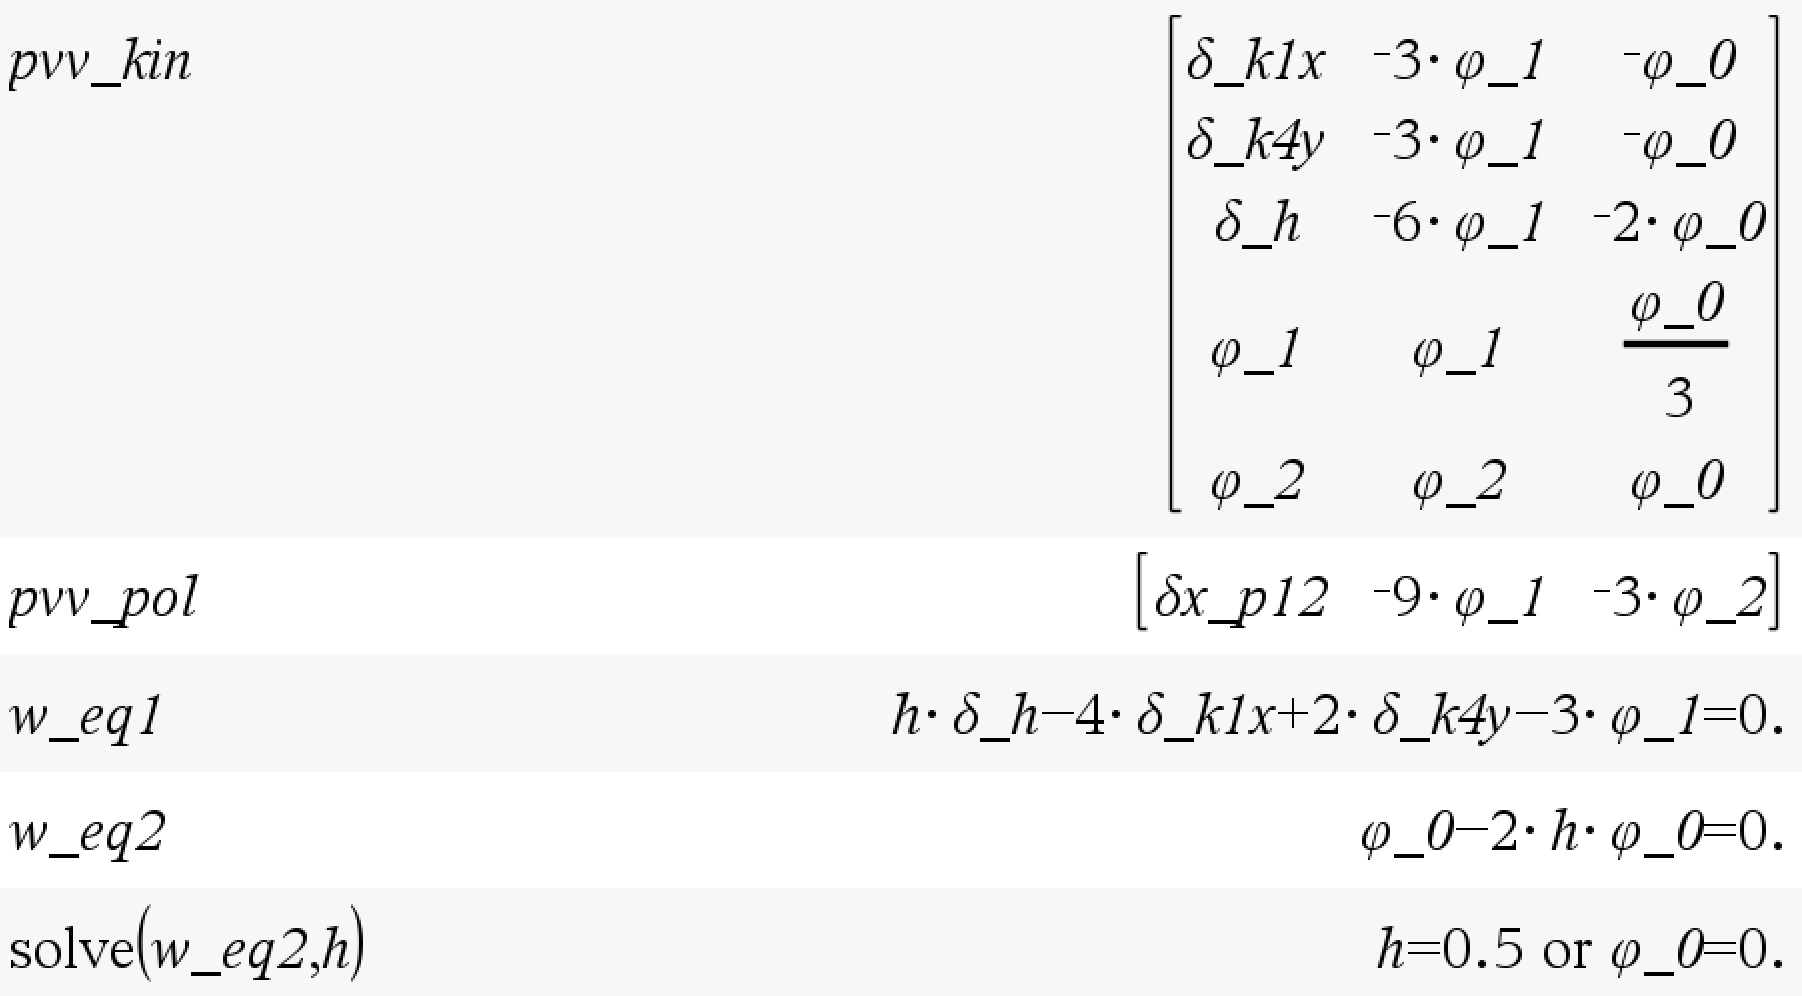
\includegraphics[width=\linewidth]{./fig/TM1/WiSe2122nr3_6.png}
        \caption{Rechnung für $A_H$}
    \end{subfigure}
    \hfill
    \begin{subfigure}[t]{0.48\textwidth}
        \centering
        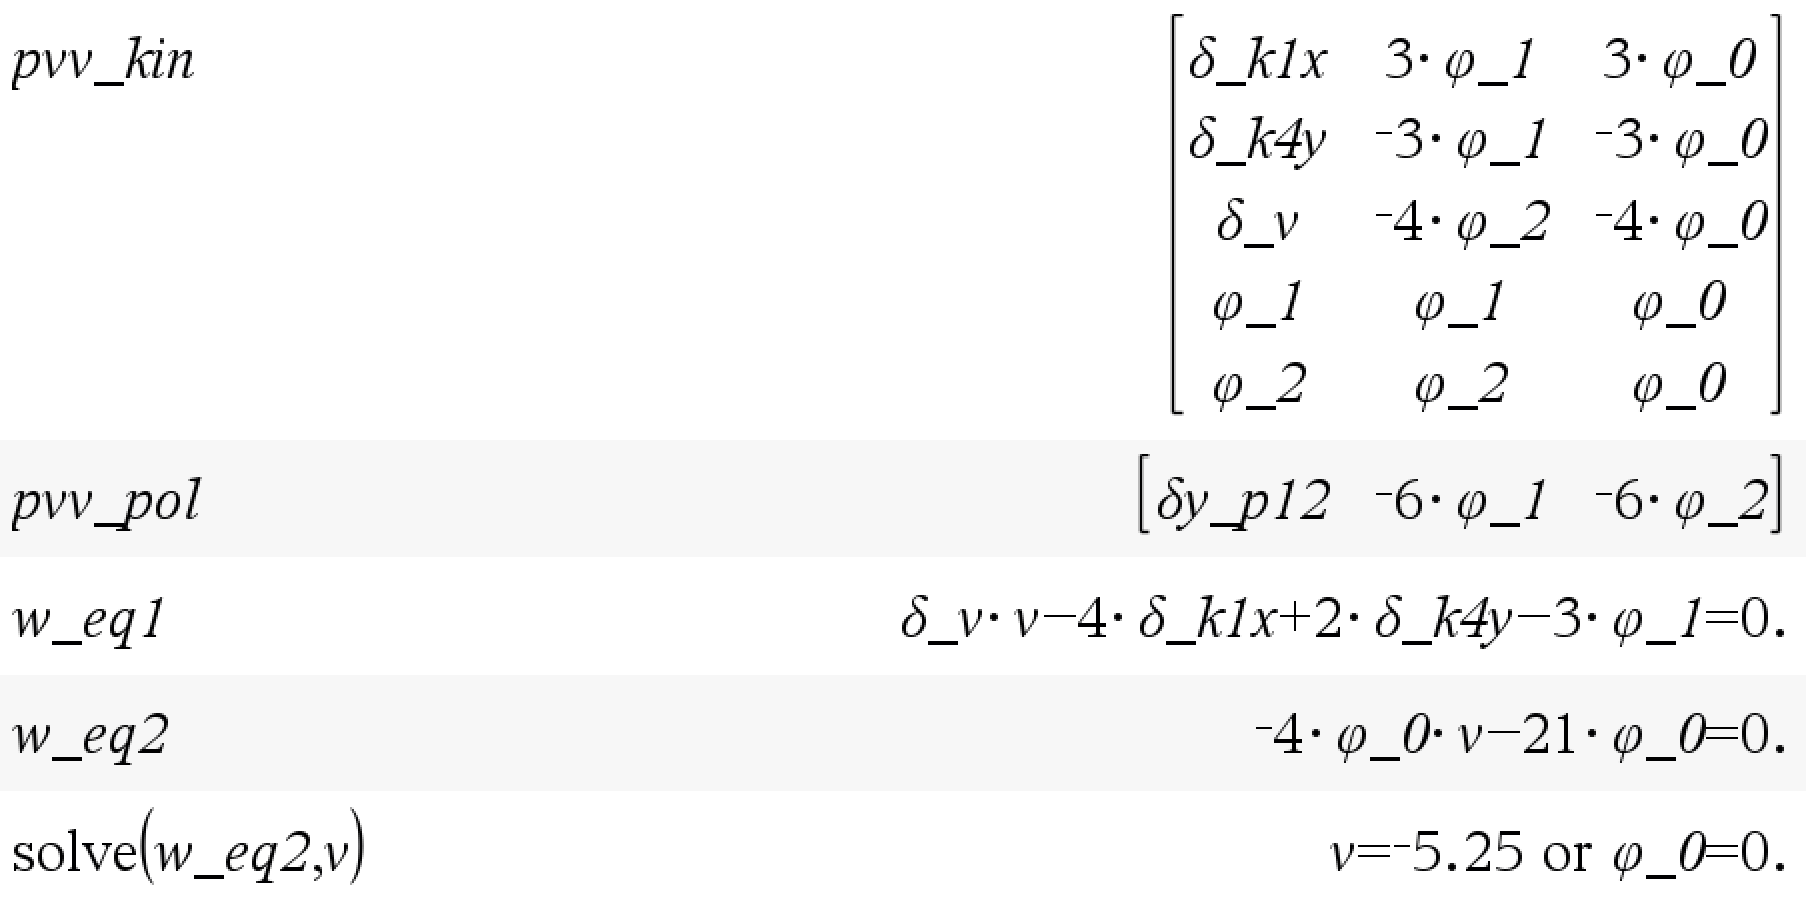
\includegraphics[width=\linewidth]{./fig/TM1/WiSe2122nr3_7.png}
        \caption{Rechnung für $B_V$}
    \end{subfigure}
    \caption{WiSe~21/22, Nr.~3: Ergebnis}
    \label{fig:TM1WiSe2122Nr3_4}
\end{figure}

\subsection{Schnittkräfte Bögen (Nr.~5)}

Mit dem Programm lassen sich die Funktionen für Schnittkraftverläufe von normalen Stäben als auch von Bögen 
ausgeben. Bei bögen ist die Laufvraibale nur nicht mehr die Länge entlang des Stabes sondern der Winkel.
also für diese Aufgabe zweilmal $\varphi \in [0,\frac{\pi}{4}]$ bzw. $\varphi \in [0,90\text{°}]$. Hier ist die Winkel-Einstellung
des Taschenrechenrs wichtig.\\
Hier gilt aber auch wieder, dass das Programm das nicht wirklich so ausrechnet wie man das von Hand machen würde, sondern
es sucht eine schöne Darstellung der Anfangswerte und kombiniert diese dann zur Funktion.

\begin{figure}[htbp]
    \centering
    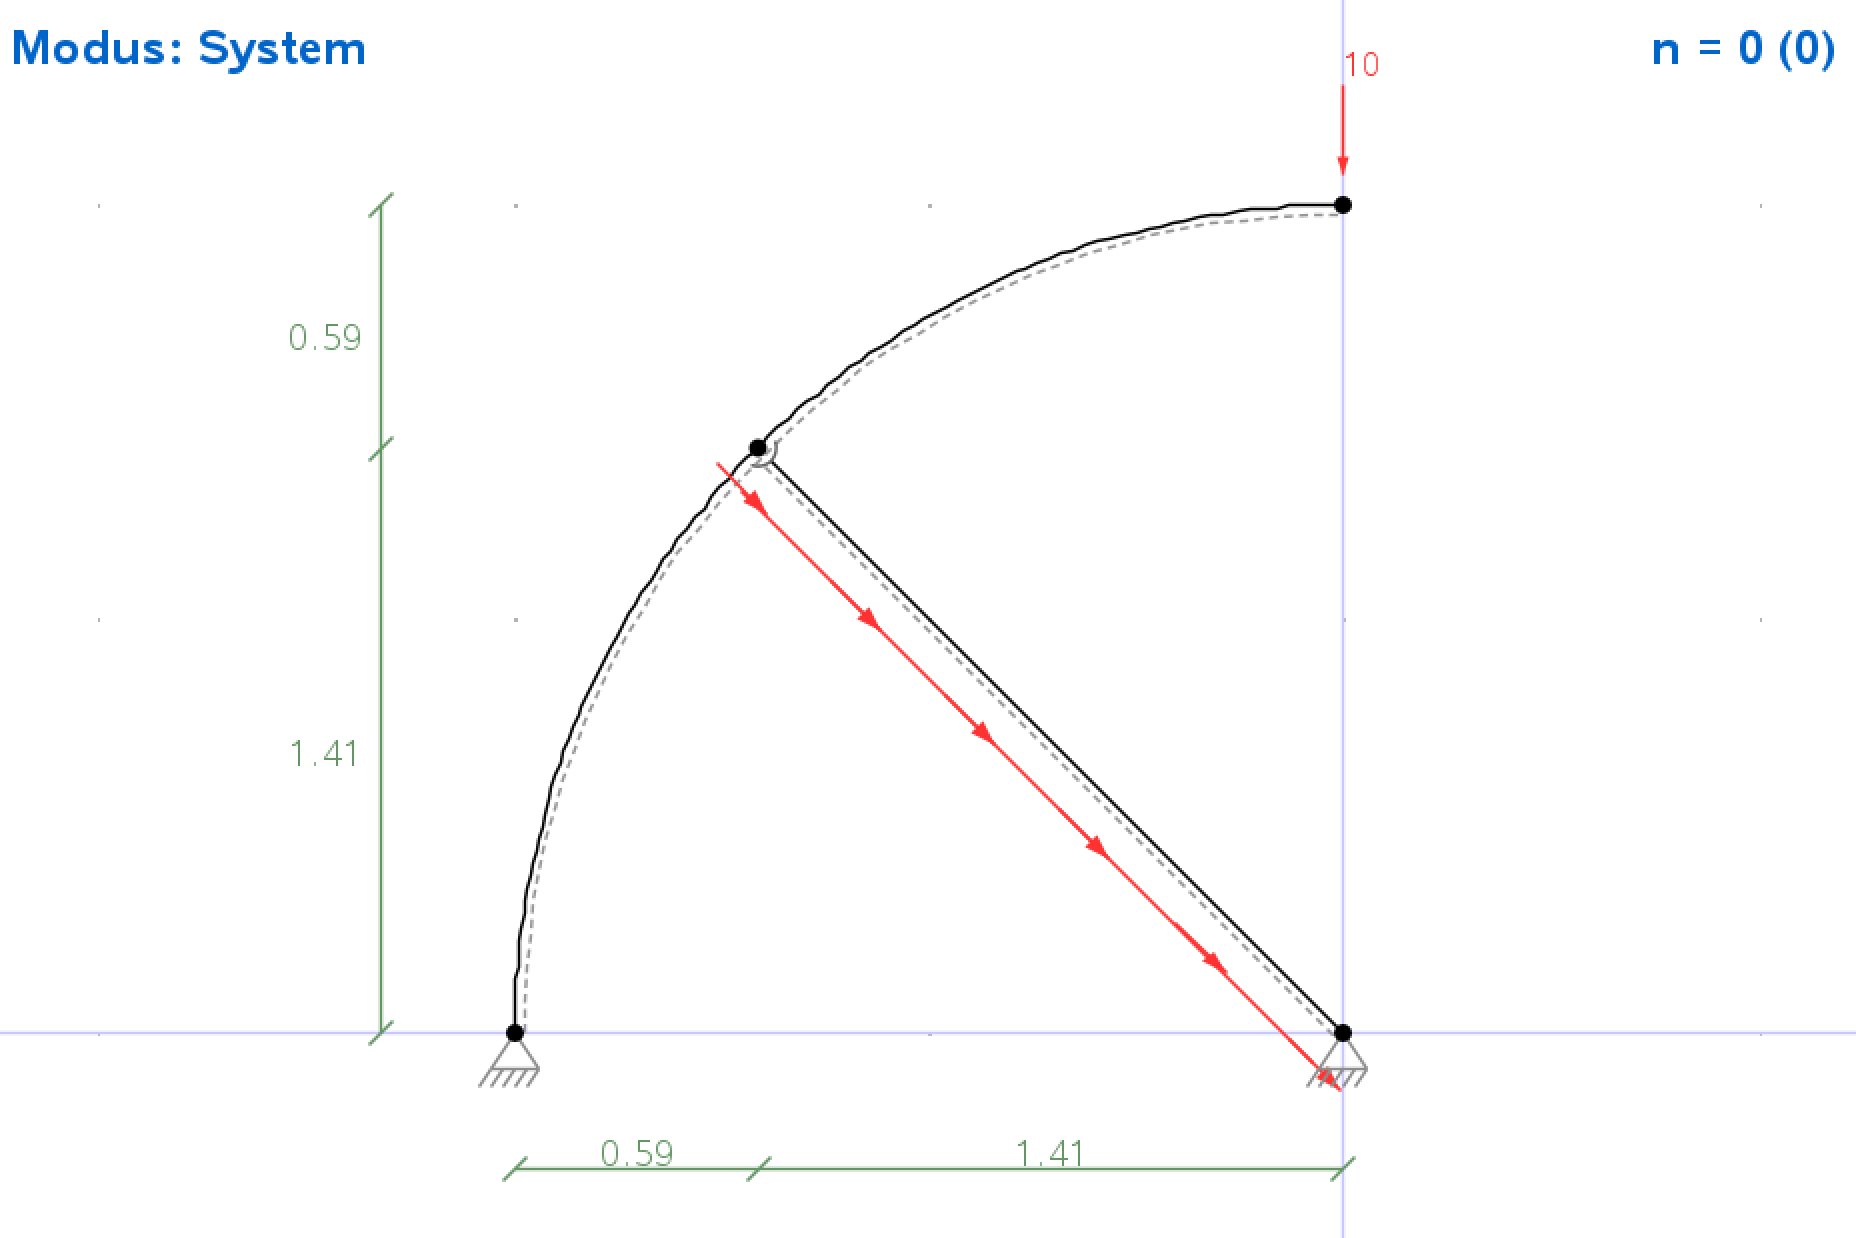
\includegraphics[width=0.5\linewidth]{./fig/TM1/WiSe2122nr5_1.png}
    \caption{TM1 WiSe~21/22, Nr.~5 im Programm}
    \label{fig:TM1WiSe2122Nr5_1}
\end{figure}


\subsection{Fachwerk (Nr.6)}

Vom Prinzip werden Fachwerke genau gleich eingegeben wie normale Systeme, nur das hier die orientierung der gestrichelten Faser
keine Rolle spielt. Es ist jedoch sinnvoll den Fachwerk Modus anzumachen, dann wird die statische Bestimmtheit beim hovern über $n=$ 
auch die Formel für Fachwerke verwendet und alle Knoten werden zu vollgelenken gemacht, auch wenn der Modus erst nach dem 
zeichnen des Systems angemacht wird.  


\begin{figure}[htbp]
    \centering
    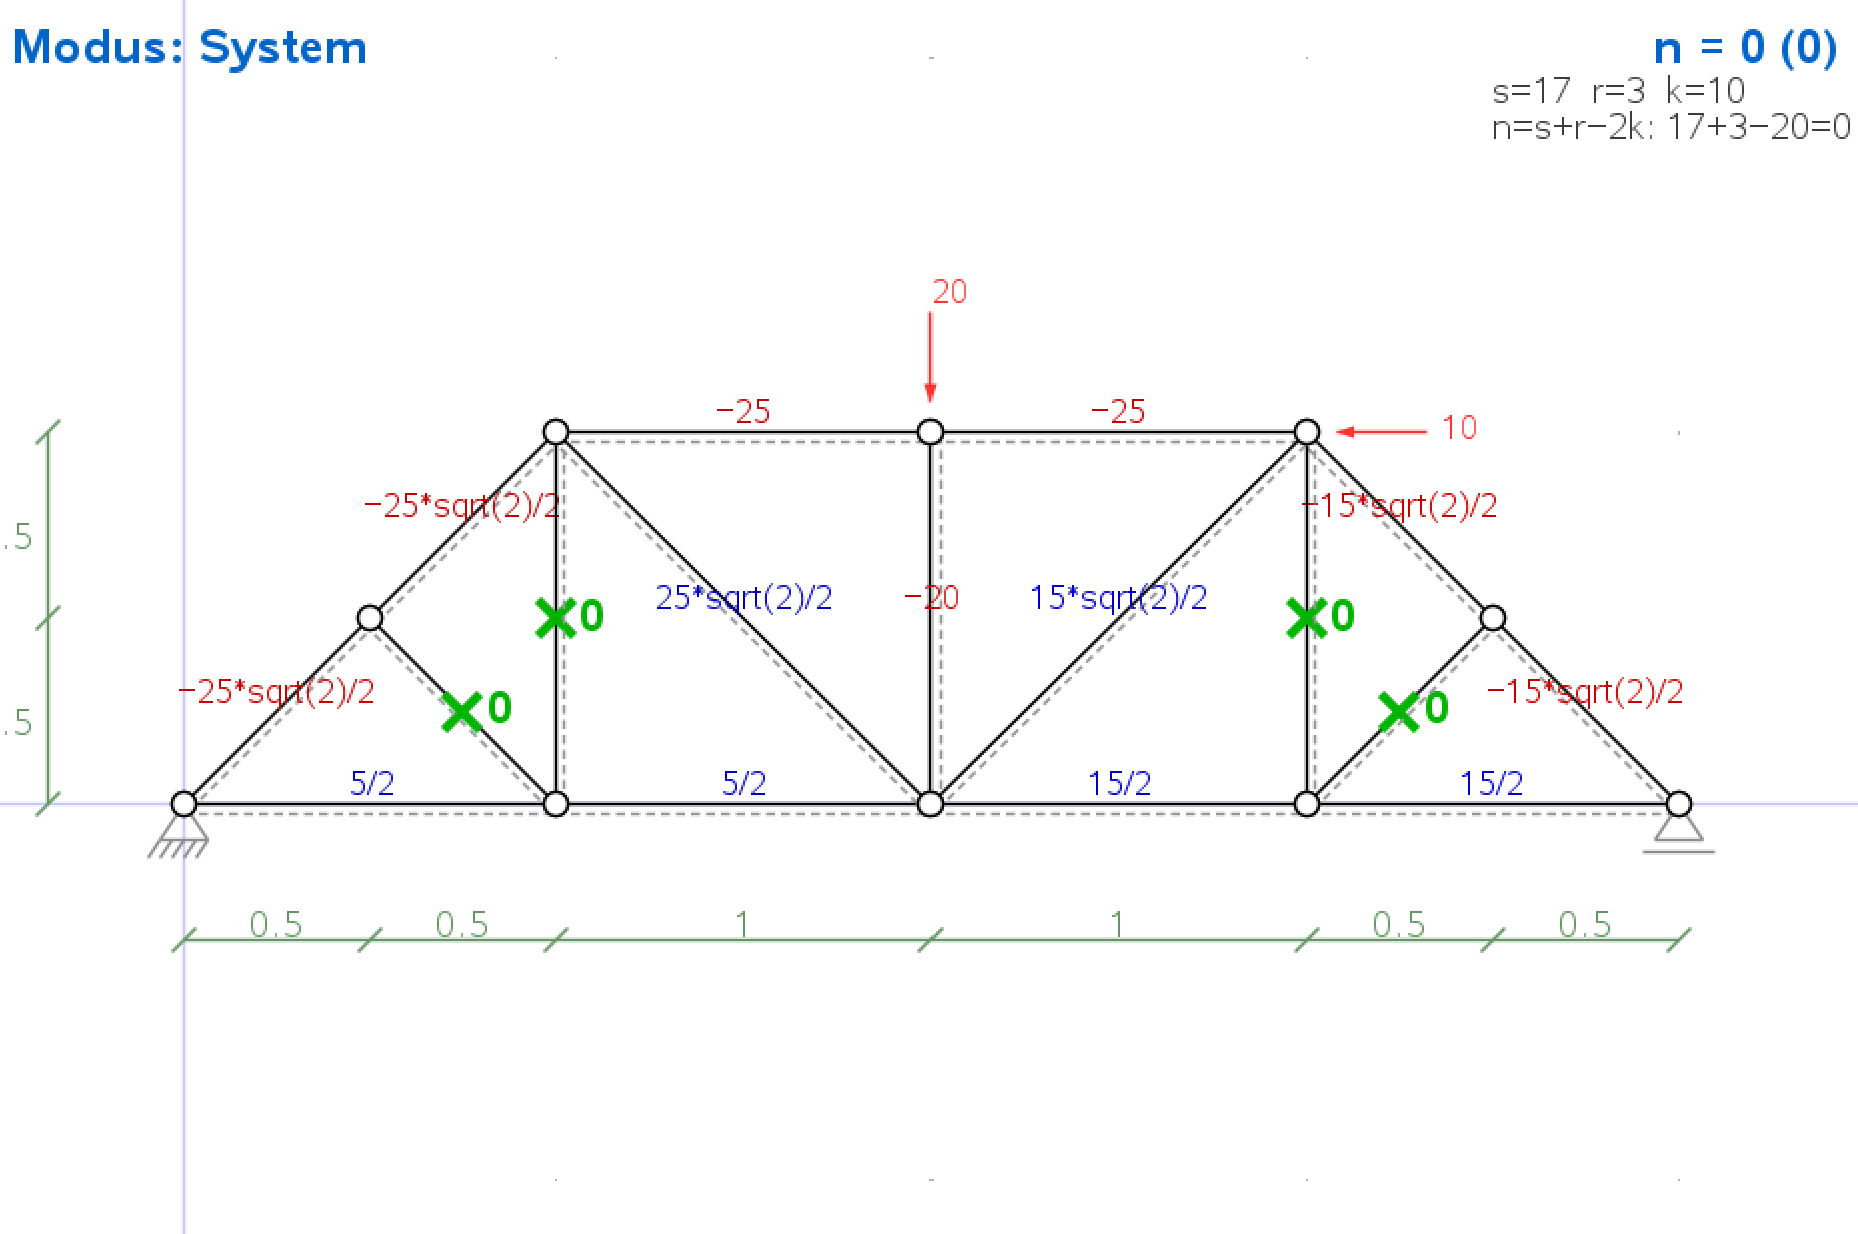
\includegraphics[width=0.5\linewidth]{./fig/TM1/WiSe2122nr6_1.png}
    \caption{TM1 WiSe~21/22, Nr.~6 im Programm}
    \label{fig:TM1WiSe2122Nr6_1}
\end{figure}

Die Stabe in Abb.~\ref{fig:TM1WiSe2122Nr6_1} die ein grünes Kreuz haben sind die ohne Rechnung erkennbaren Nullstäbe
Falls nach der Berechnung stäbkkräfte mit einer grünen Null beschriftet werdsen, aber dort kein Kreuz ist, ist das zwar ein 
Nullstab der aber nicht direkt aus den Regeln erkennbar ist. Für Afgaben bei denen nach Nullstäben gefragt wird, also nur 
die durchgekreuzten Stäbe angeben

\begin{figure}[htbp]
    \centering
    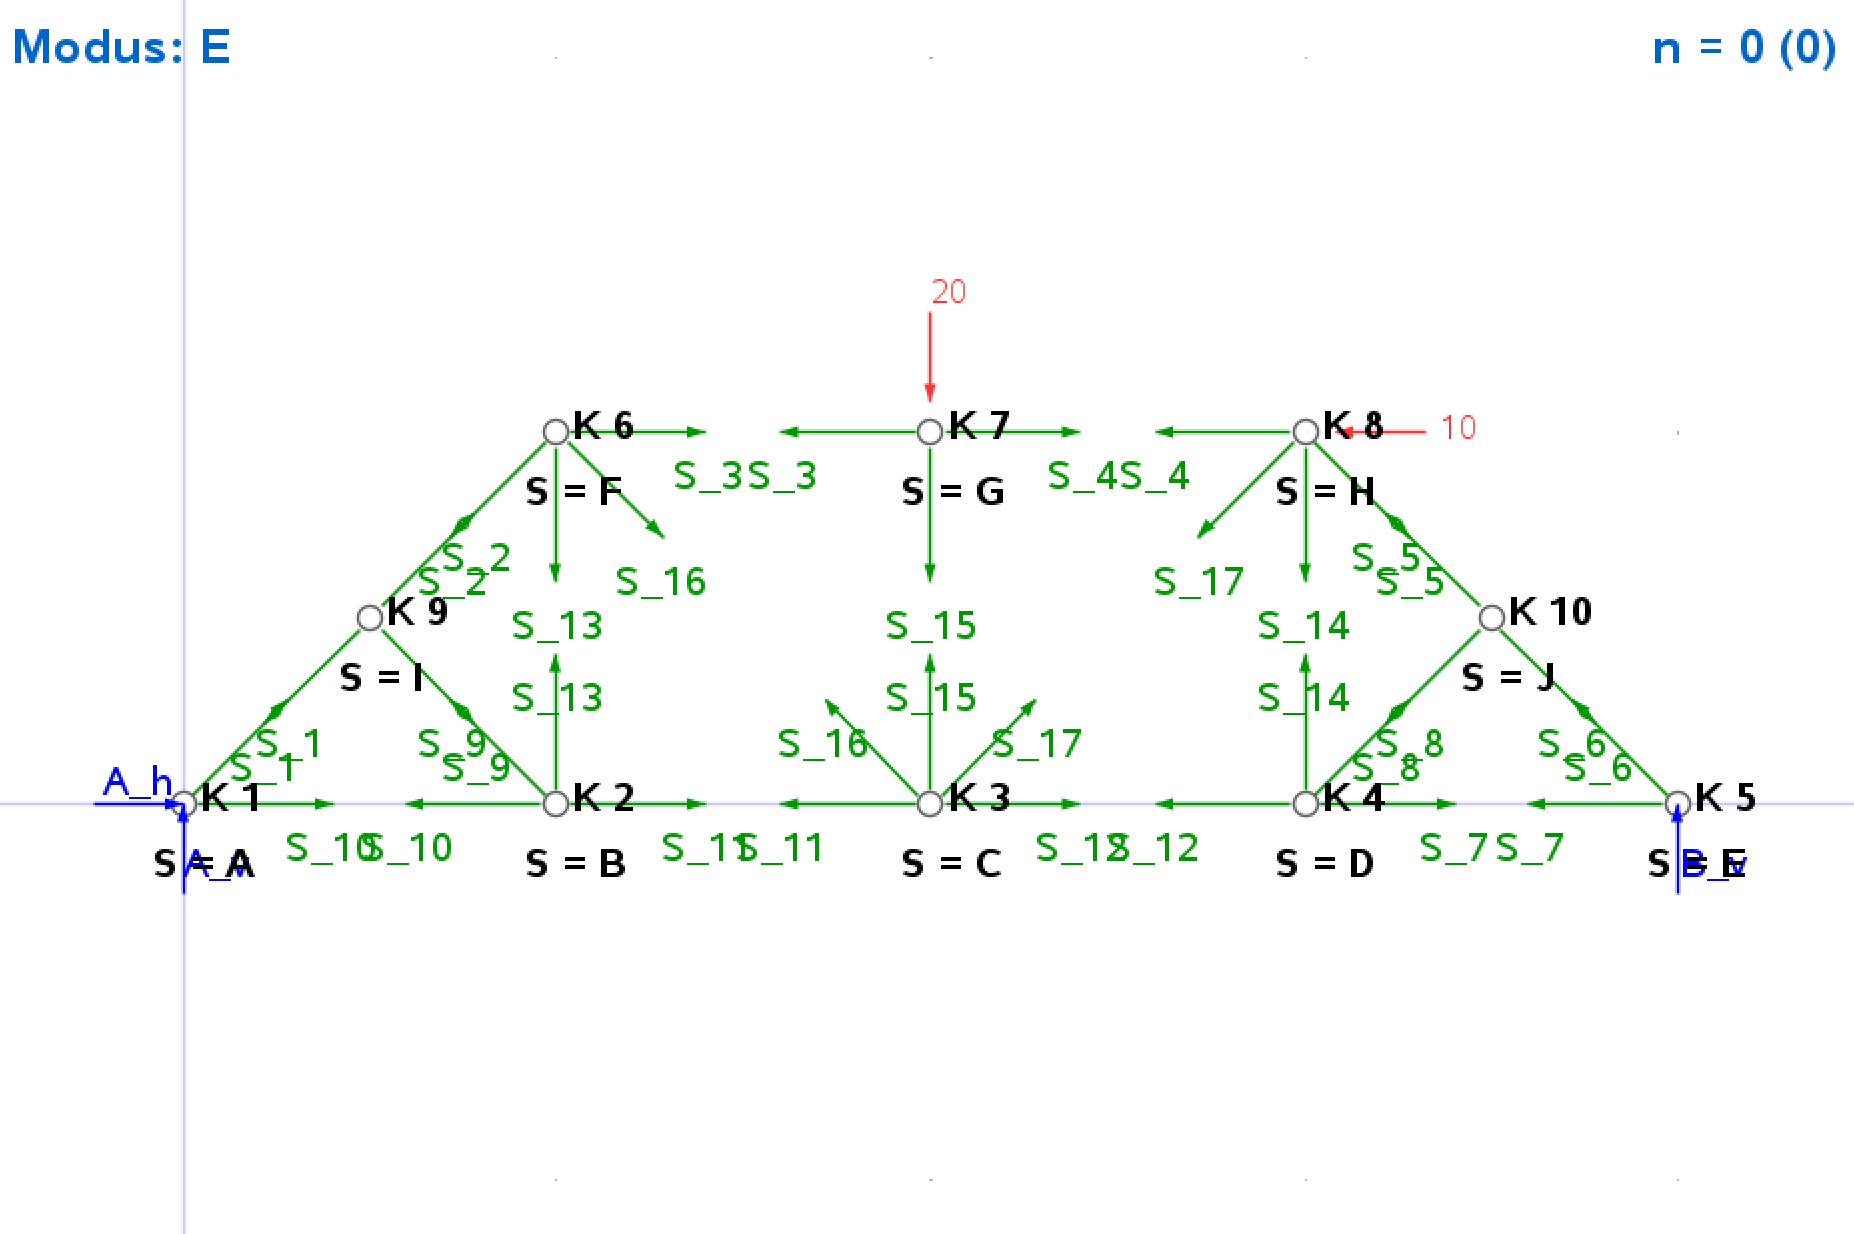
\includegraphics[width=0.5\linewidth]{./fig/TM1/WiSe2122nr6_2.png}
    \caption{TM1 WiSe~21/22 Freischnitt}
    \label{fig:TM1WiSe2122Nr6_2}
\end{figure}

Für die Verwendung der beiden Seiten des E-Modus muss darauf geachtet werden, dass entweder die Stäbe in der
gleichen Reihenfolge wie in der Aufgabe gezeichnet werden oder die Bennenung hinterher angepasst wird. Macht ihr das nicht
ist z.B. Stab 13 aus eurer Rechnung nicht Stab 13 aus der Aufgabe\\
Gleiches gilt natürlich auch für die Verwendung des LGS-Exports. Hier wird (Falls der Fachwerk Modus an ist) 
das Knotenschnittverfahren verwendet. Die Benennung im LGS ist die gleiche wie auf der zweiten Seite des E-Modus.





\section{TM2}

\subsection{Biegelinie (TM2 WiSe~21/22, Nr.~7)} \label{ex:Biegelinienaufgabe}

In dieser Aufgabe ist ein \emph{interessantes} KOS vorgegeben: Soll es ein Rechtssystem sein,
zeigt die $y$-Achse hier in die Zeichenebene hinein und nicht, wie sonst üblich, aus ihr heraus.

Rechnet ihr von Hand über die DGL $EI\,w'''' = q$ mit allen Rand- und Übergangsbedingungen (so
geht man bei statisch unbestimmten Systemen meist vor, und so rechnet auch \code{wneu}), gibt es
hier nichts weiter zu beachten. Bei einem statisch bestimmten System lohnt es sich dagegen, zuerst
die Momentenlinie zu berechnen und dann $EI\,w'' = -M$ zu integrieren. Dafür braucht ihr die
gestrichelte Faser. Die Regel aus Abschnitt~\ref{sec:Eingabe_Stäbe}, dass sie immer auf der Seite
liegt, in die die $z$- bzw.\ $w$-Achse zeigt, gilt auch hier. Alternativ könnt ihr euch überlegen,
auf welcher Seite ein positives Schnittmoment $M_y$ (Drehsinn nach der Rechte-Hand-Regel um die
$y$-Achse) Zug erzeugt, dort liegt die gestrichelte Faser. Das finde ich aber umständlicher.

Im Programm müsst ihr solche Systeme etwas anders eingeben, denn dort zeigt die $y$-Achse immer
aus der Zeichenebene heraus. Zeichnet ihr das System genau wie in der Aufgabe und setzt die
gestrichelte Faser nach der Regel oben, läuft die $x$-Koordinate im Programm in die andere Richtung
als in der Aufgabe. Um das zu umgehen, zeichnet ihr Systeme, bei denen die $y$-Achse in die
Zeichenebene hineinzeigt, spiegelverkehrt (Abb.~\ref{fig:Biegelinienaufgabe}). Ich habe die
Aufgabe im symbolischen Modus gerechnet, deshalb stehen in den Ergebnissen $q$ und $l$.

\begin{figure}[htbp]
    \centering
    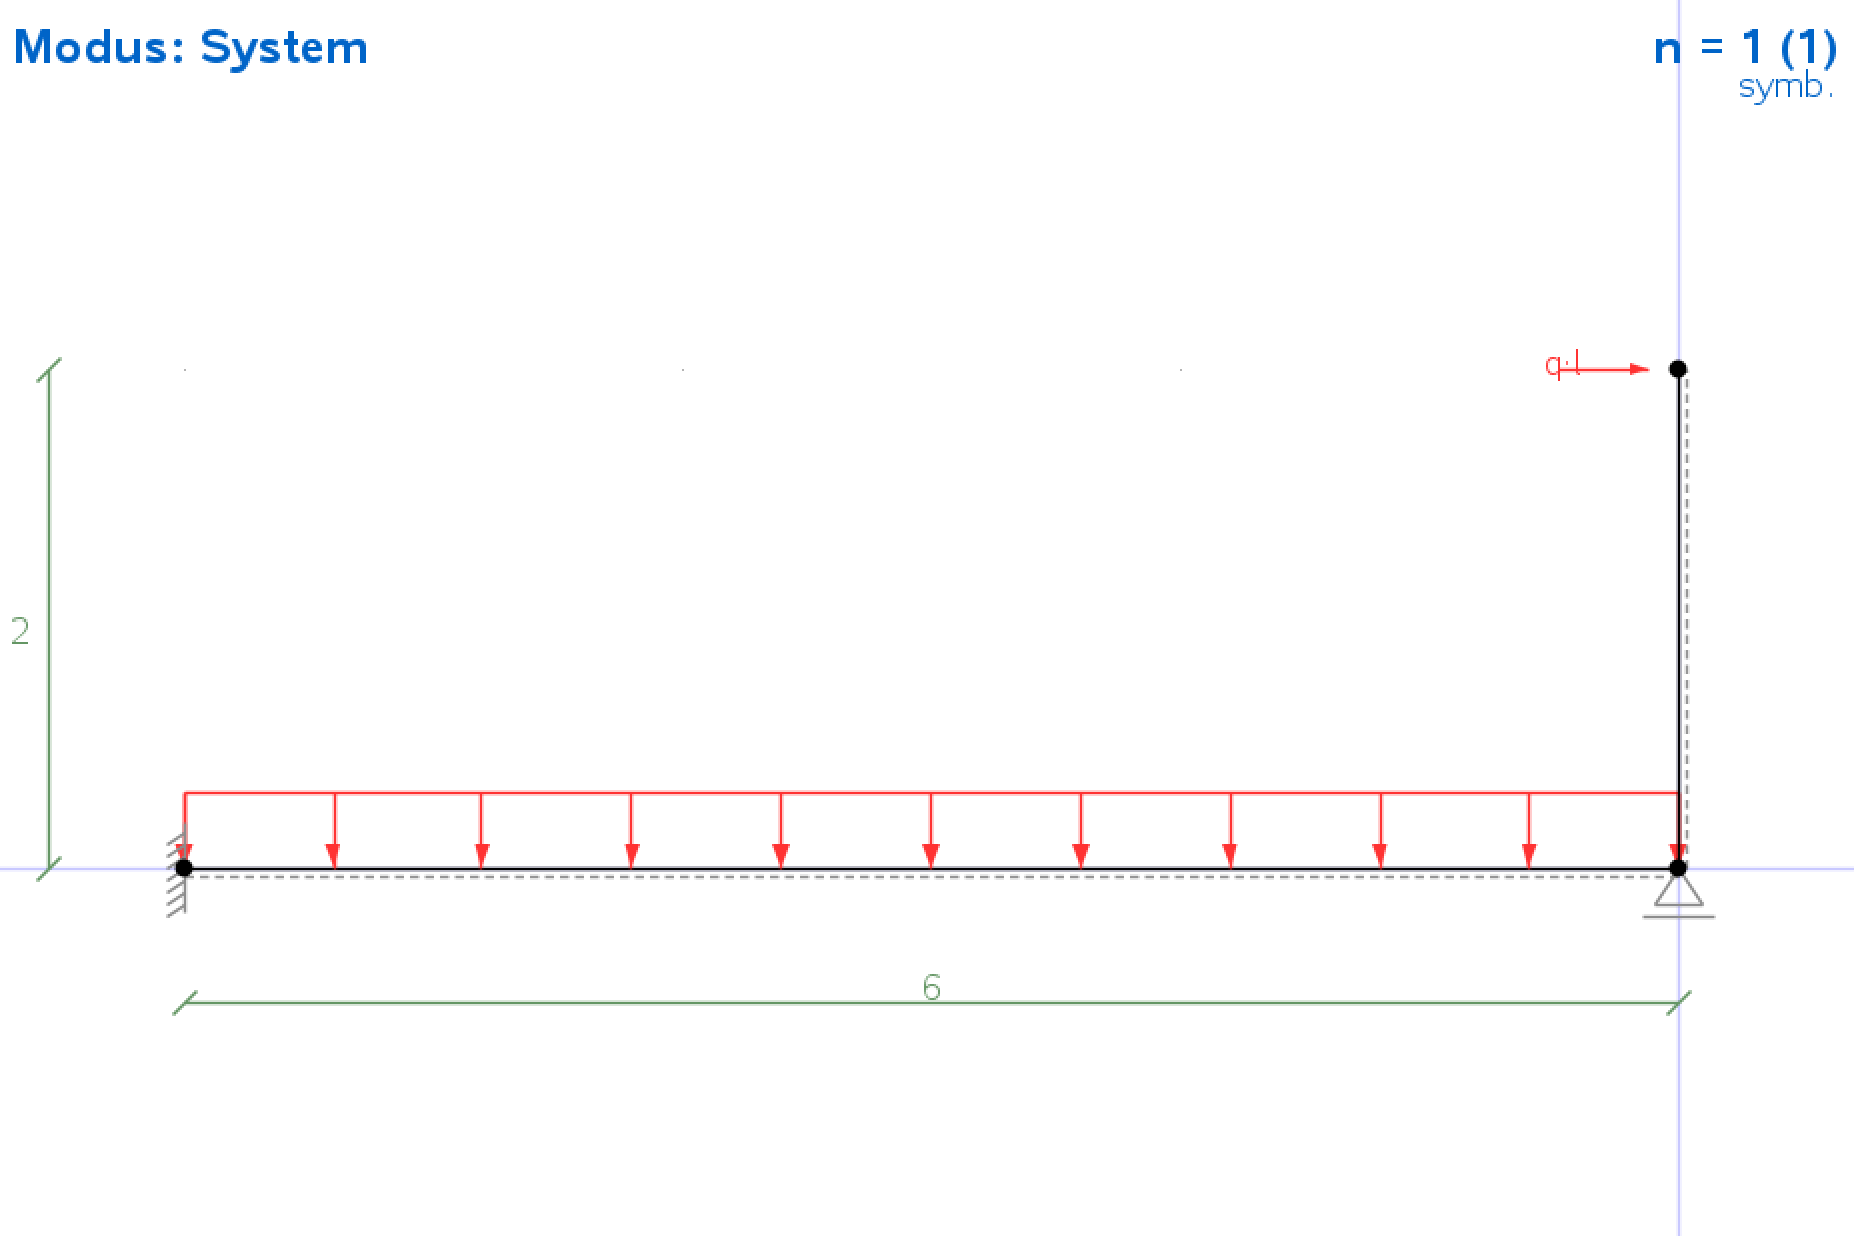
\includegraphics[width=0.5\linewidth]{./fig/TM2/WiSe2122nr7_1.png}
    \caption{TM2 WiSe~21/22, Nr.~7 im Programm, spiegelverkehrt gezeichnet}
    \label{fig:Biegelinienaufgabe}
\end{figure}

Das liefert die Ergebnisse in Abb.~\ref{fig:BiegelinienaufgabeBiegelinie}. Hier geben beide
Methoden dasselbe Ergebnis. Das sollte natürlich so sein, ist aber nicht immer so: Manchmal weicht
die WGV/FEM-Lösung \code{v\_EI\_stab1(x)} (im Rechner klein geschrieben) minimal von der exakten
Lösung \code{wneu1(x)} ab. Weil das Programm die Brüche aus den Zahlen der FEM-Lösung
\emph{errät} (Abschnitt~\ref{sec:mathe-symbolisch}), kann daraus eine ganz anders aussehende
Biegelinie werden. Die Methode über die WGV/FEM-Lösung gibt es trotzdem, vor allem weil ich sie
zuerst programmiert habe (daher wohl auch der Name \code{wneu} der anderen Funktion), und weil sie
bei sehr großen Systemen deutlich schneller sein kann.

\begin{figure}[htbp]
    \centering
    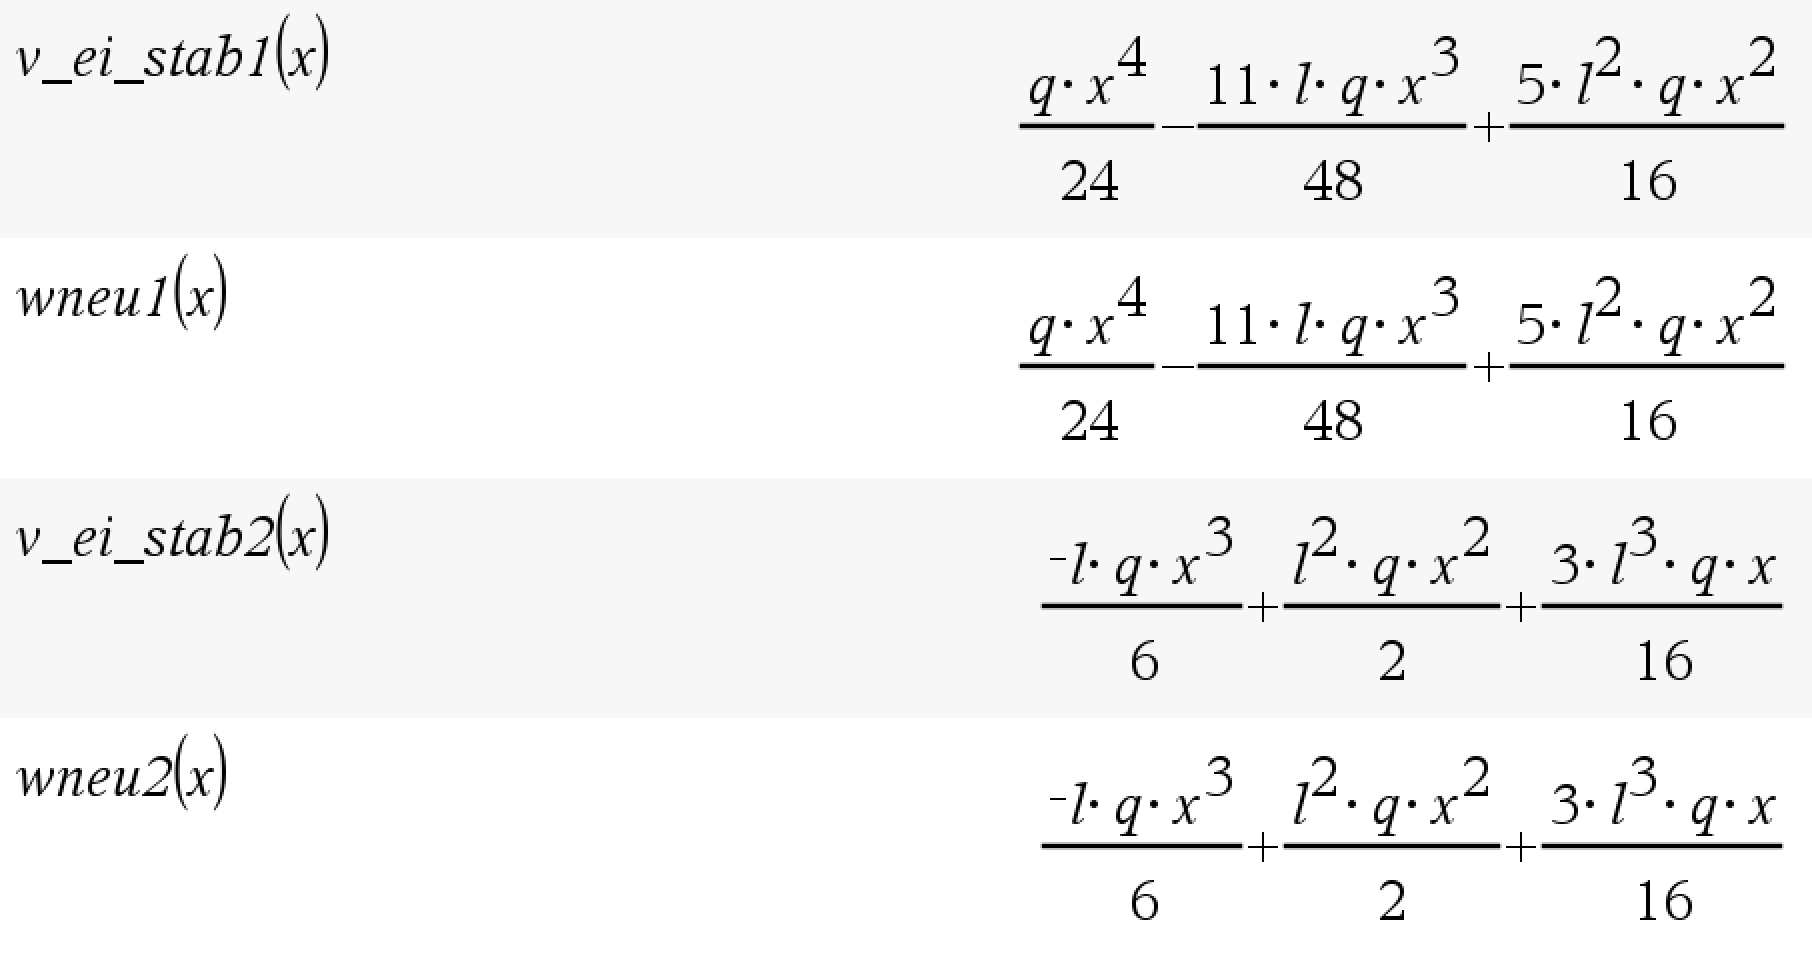
\includegraphics[width=0.5\linewidth]{./fig/TM2/WiSe2122nr7_2.png}
    \caption{TM2 WiSe~21/22, Nr.~7: \code{v\_EI\_stab} und \code{wneu} im Vergleich}
    \label{fig:BiegelinienaufgabeBiegelinie}
\end{figure}

Weil die Stäbe dehnsteif sind, kann das Programm hier sogar die Randbedingungen für Biegelinie und
Längslinie getrennt angeben (Abb.~\ref{fig:BiegelinienaufgabeRandbed}): Die Bedingungen im oberen
Block reichen für die Biegelinie allein, die im unteren kommen nur für die Längslinie dazu. Das geht
nicht immer. Sind die Stäbe dehnbar, hängt die Biegelinie über die Rahmenecken auch von den
Längsverformungen ab, und das Programm gibt alle Bedingungen zusammen aus
(Abschnitt~\ref{sec:randlgs}).

\begin{figure}[htbp]
    \centering
    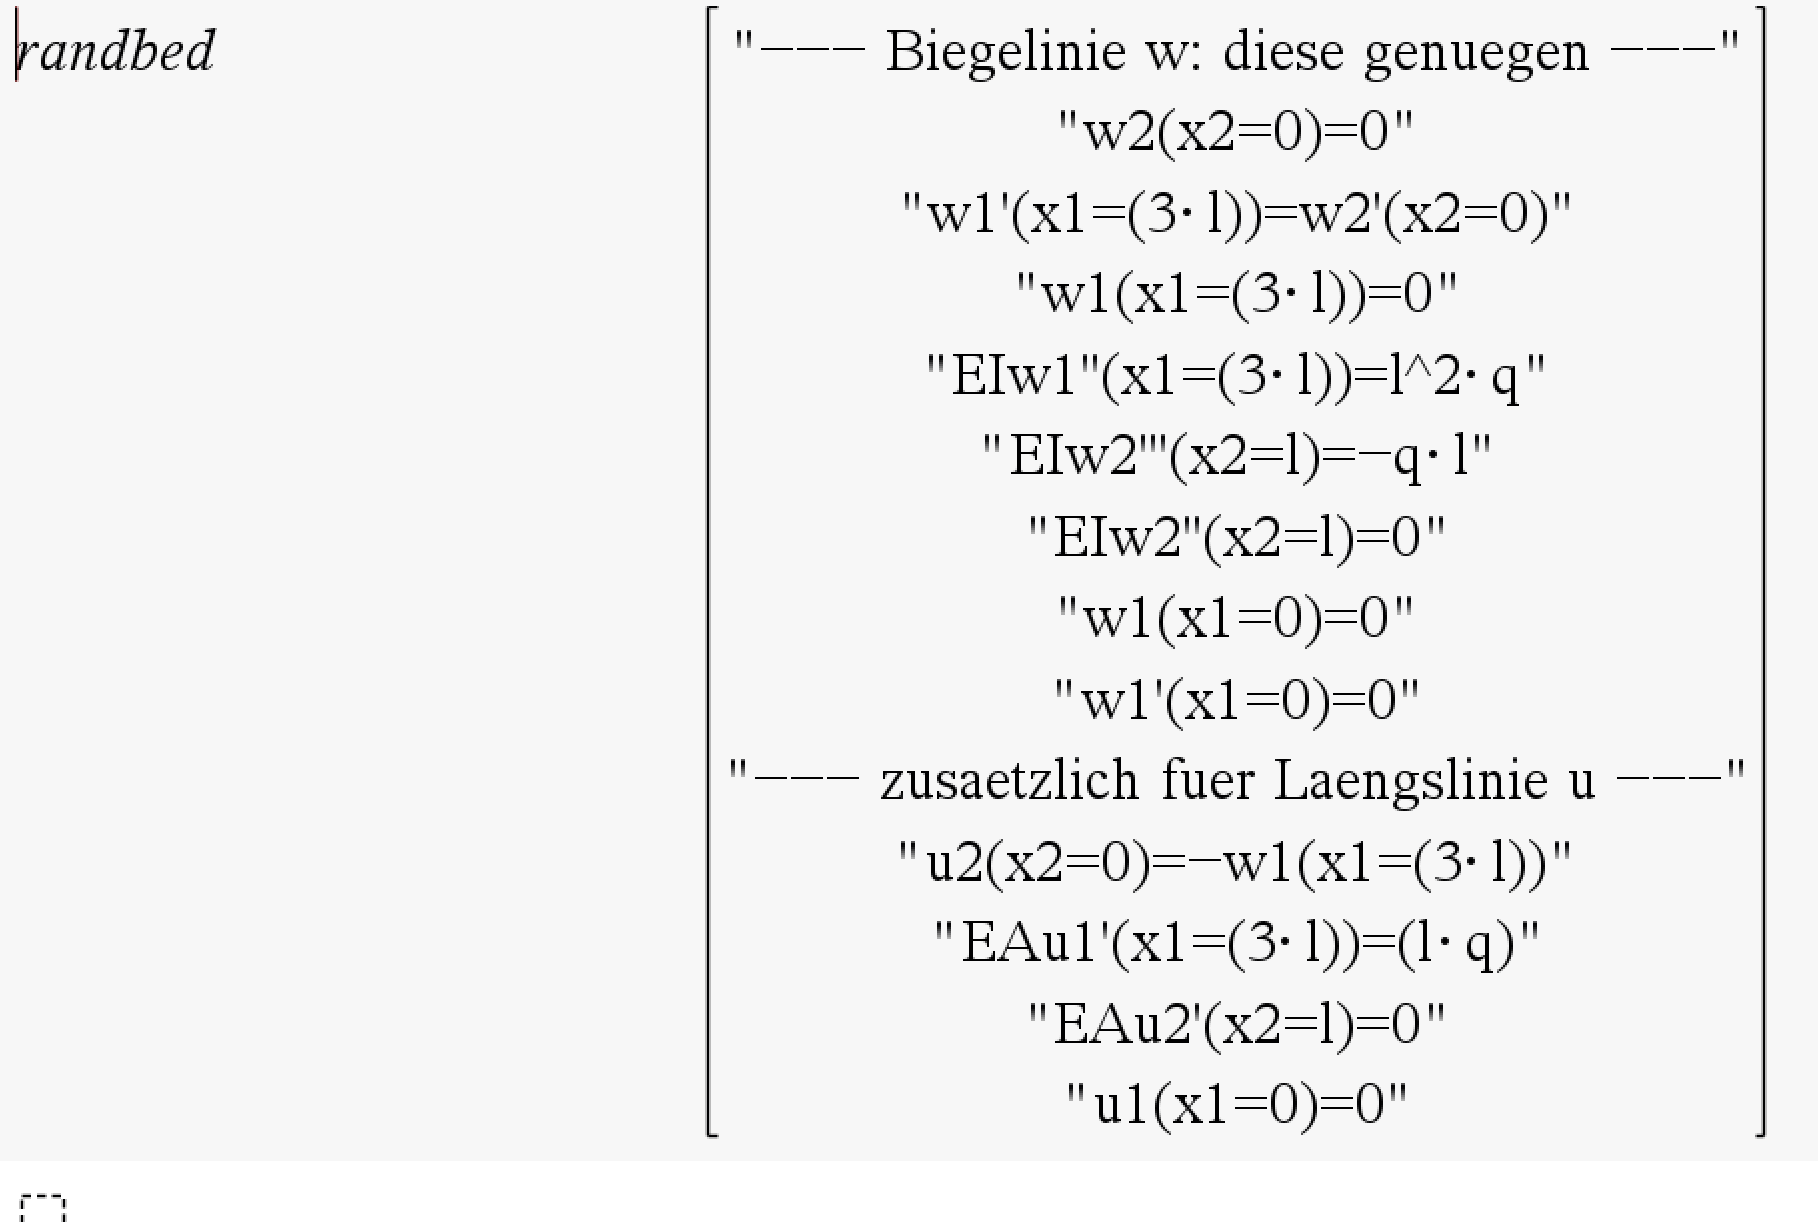
\includegraphics[width=0.5\linewidth]{./fig/TM2/WiSe2122nr7_3.png}
    \caption{Randbedingungen \code{randbed} für TM2 WiSe~21/22, Nr.~7}
    \label{fig:BiegelinienaufgabeRandbed}
\end{figure}



\subsection{Verschiebungsaufgaben (TM2 WiSe~20/21 Nr.~4)} \label{ex:Temperaturaufgabe}

Aufgaben wie diese lassen sich mit der richtigen Eingabe auch direkt im Programm lösen. Wie diese Aufagbe im
Programm aussieht ist in Abb.~\ref{fig:verschiebungSystem} dargestellt. Hierbei muss natürlich auf die Einheiten geachtet werden.
In der Aufgabe sind die relevanten Dehnsteifigkeiten nicht direkt gegeben, genauso wie manche Angaben nicht in der
für das Programm geforderten Einheit sind.\\
Für Kräfte immer kN, genauso wie für die Dehnsteifigkeit $EA$ und die Biegesteifigkeit $EI$ in kNm.  

\begin{figure}[htbp]
    \centering
    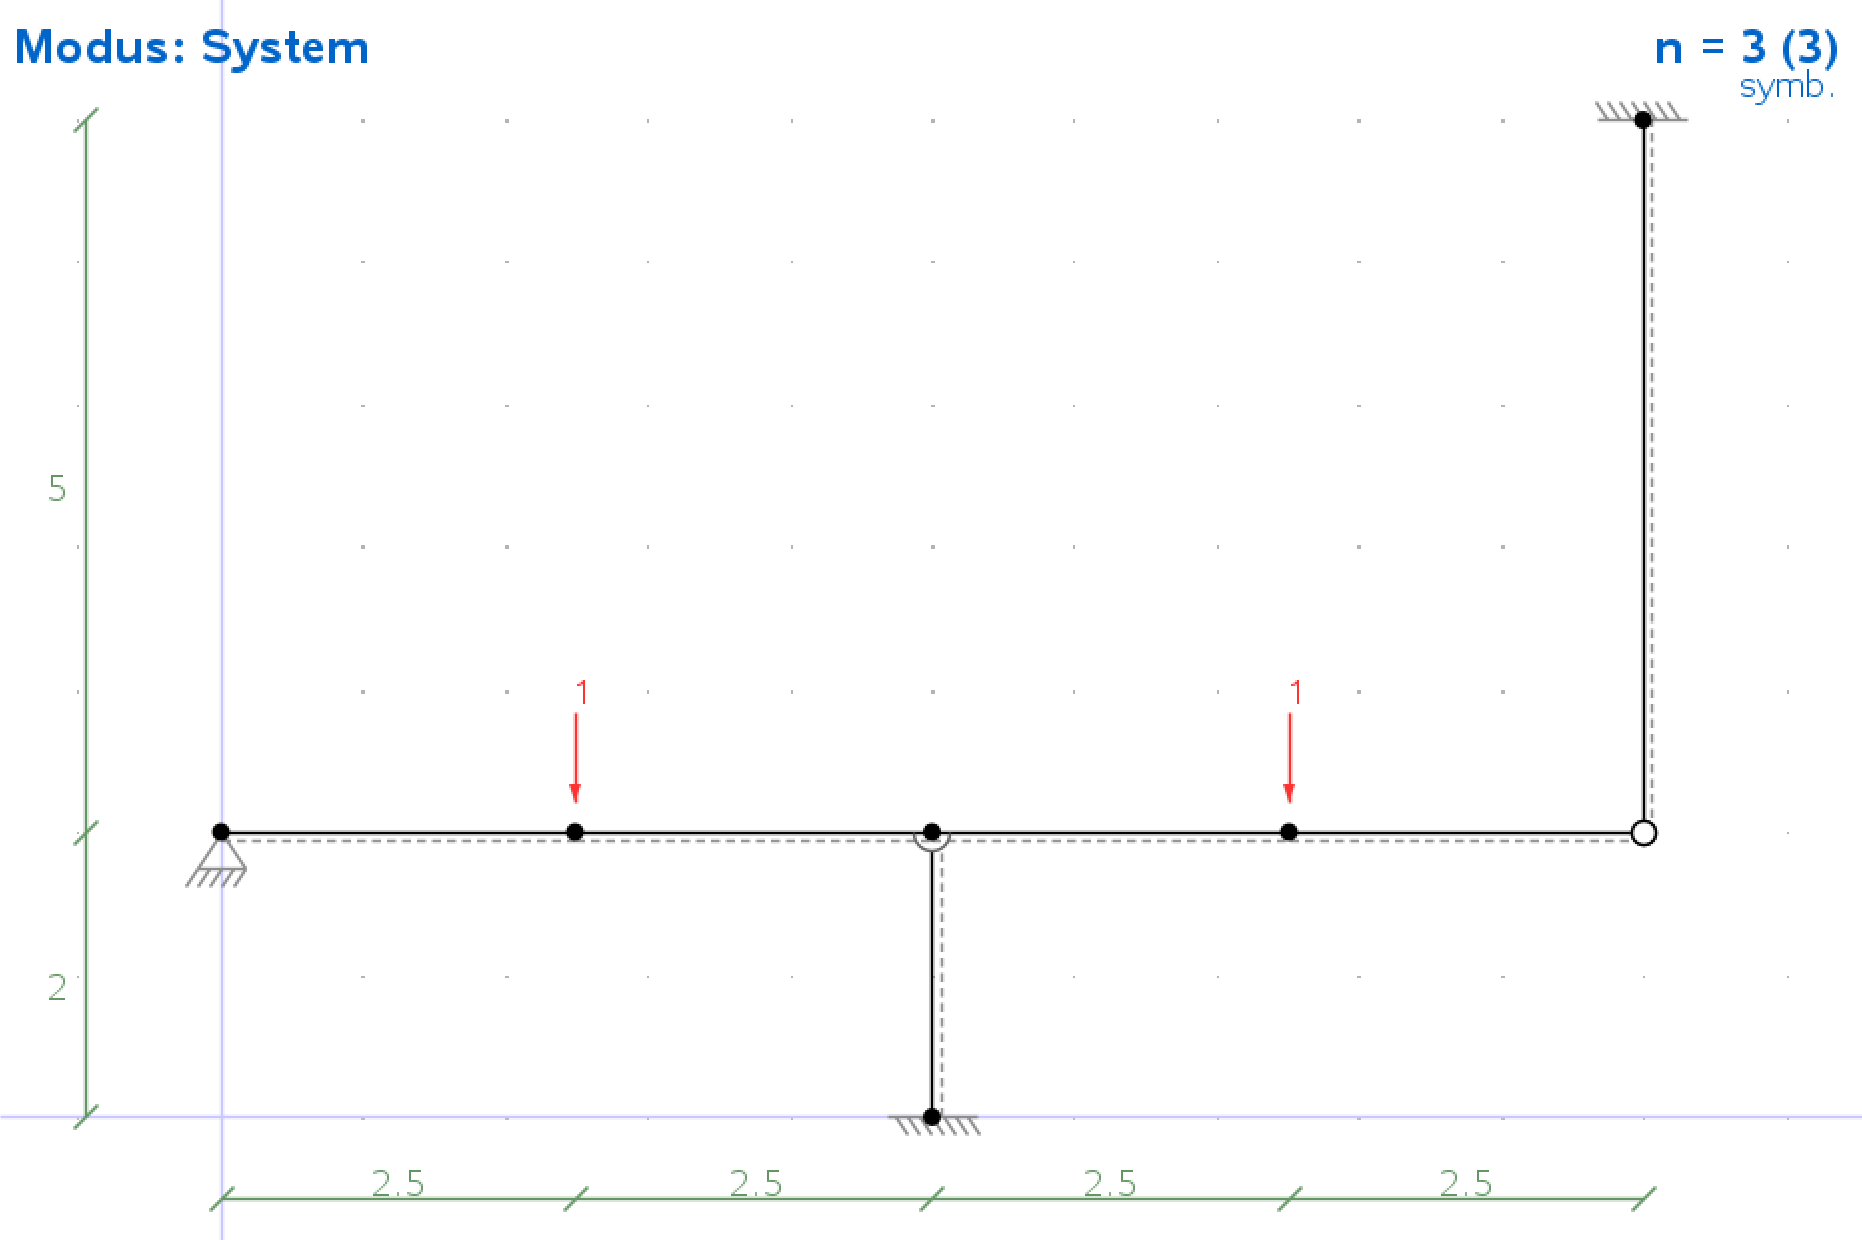
\includegraphics[width=0.5\linewidth]{./fig/TM2/WiSe2021nr4_1.png}
    \caption{TM2 WiSe~20/21, Nr.~4a im Programm}
    \label{fig:verschiebungSystem}
\end{figure}

In den \emph{neuen} Exportfunktionen wird die Temperatur auch symbolisch miteinberechnet.
Um also ann die Verschiebung des rechten unteren Knoten zu kommen lässt sich das entweder über die obere
Knotenexportfunktion machen, über die Biegelinie des rechten horizontalen Stabes oder über die Längsverschiebungsfunktion
des rechten vertikalen Stabes. Über den CAS Befehl \code{solve()} lässt sich die Temperatur direkt ausrechnen 
(vgl. Abb.~\ref{fig:verschiebungErgebniss}). Ich habe hier die Tempertur $dt$ genant (nur $T$ ist wie bereits erwähnt nicht erlaubt),
die Variable nach der aufgelöst werden soll muss der \code{solve()} Funktion als zweites Argument mit gegeben werden.

\begin{figure}[htbp]
    \centering
    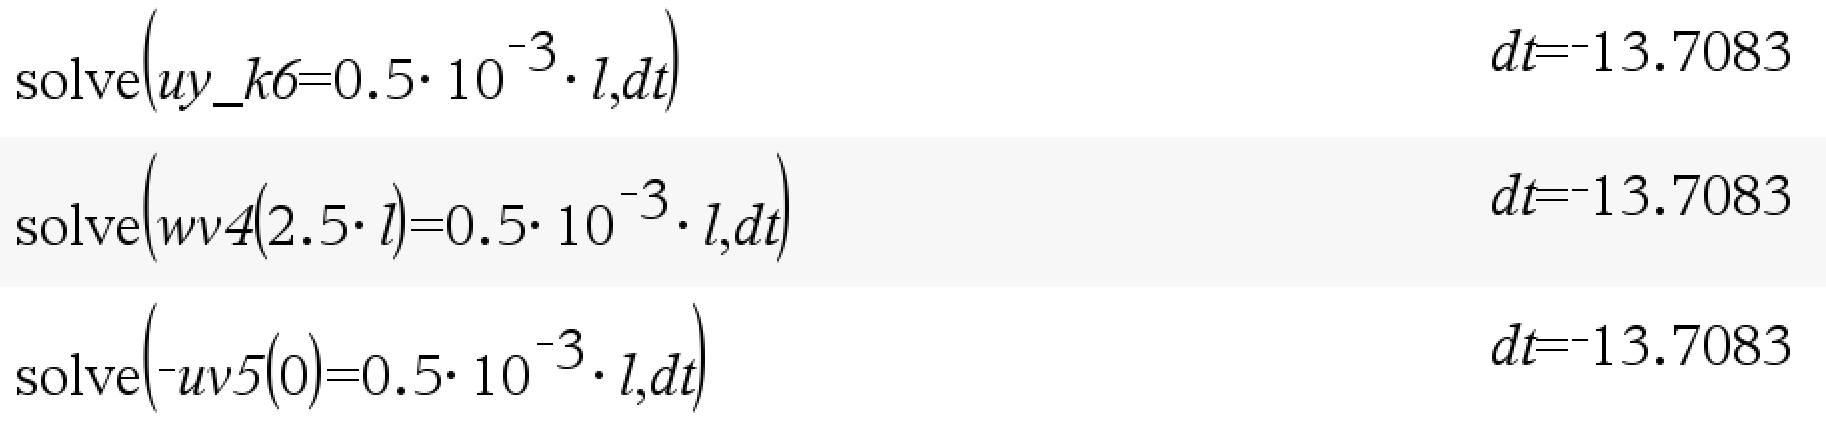
\includegraphics[width=0.5\linewidth]{./fig/TM2/WiSe2021nr4_2.png}
    \caption{Lösung von TM2 WiSe~20/21, Nr.~4a}
    \label{fig:verschiebungErgebniss}
\end{figure}

Der Zweite Teil der Aufgabe lässt sich auch im Programm lösen (Abb.~\ref{fig:VerschiebungTemp}), jedoch gibt es auch hier
ein paar Feinheiten. Ein deratiges System zu speichern kann sich lohnen. Auch hier gelten natürlich die gleichen Hinweise zu den Einheiten.

\begin{figure}[htbp]
    \centering
    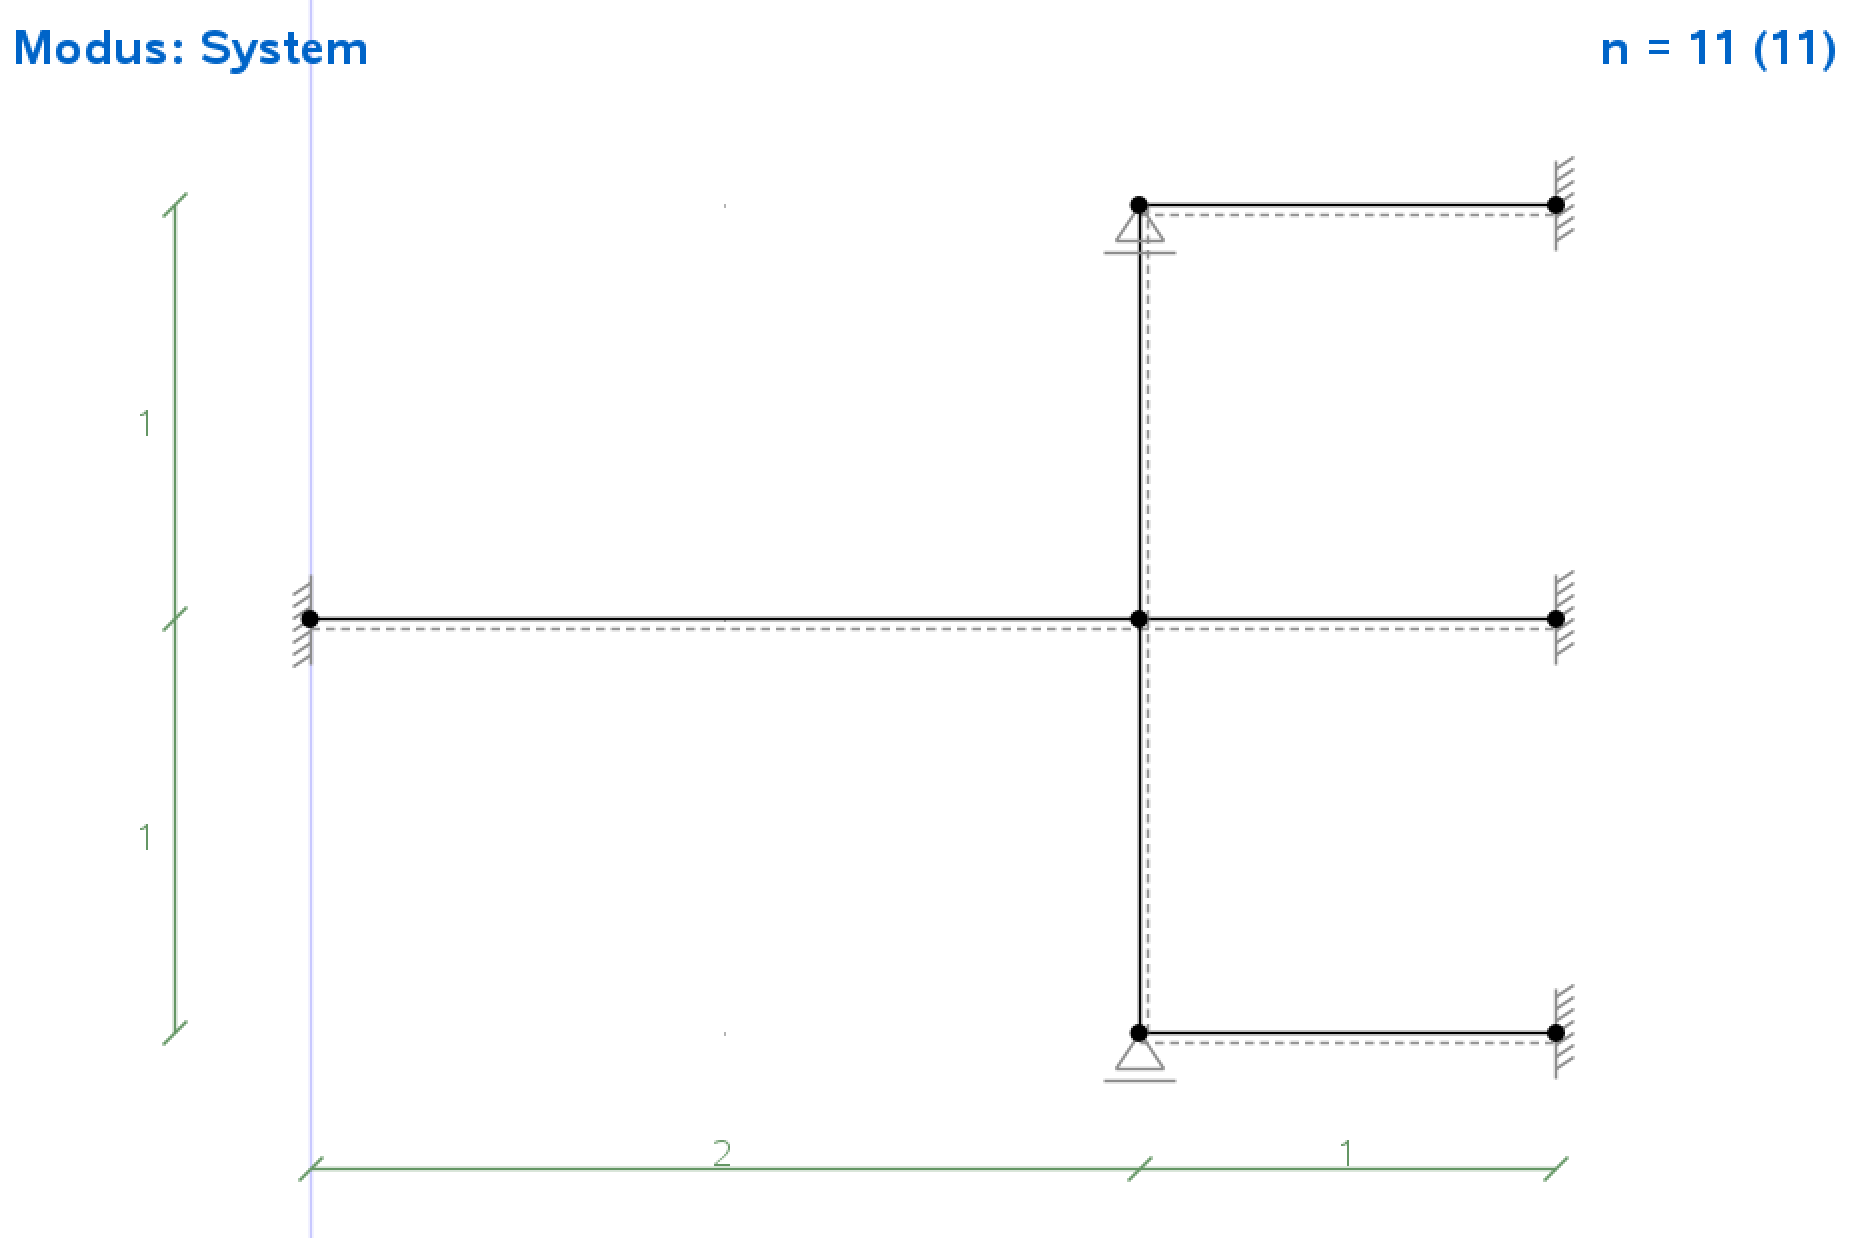
\includegraphics[width=0.5\linewidth]{./fig/TM2/WiSe2021nr4_3.png}
    \caption{TM2 WiSe~20/21, Nr.~4b im Programm}
    \label{fig:VerschiebungTemp}
\end{figure}

Da das Programm nur schnittgrößen direkt berechnet müssen diese noch in Spannungen umgerechnet werden, dafür gibt es in diesem Fall
zwei Möglichkeiten (vgl. Abb.\ref{fig:TM2WiSe2021Nr4b}). Entweder man rechnet die Spannunge direkt über die Schnittkraftverläufe aus,
oder über die Ableitung der Verschiebungsfunktion. Für die zweite Methode muss jedoch darauf geachtet werden den Temperatur Anteil
korrekt zu verrechnen.\\
Erstere Methode ist für Aufgaben mit Zahlenwerten auf jeden Fall die Einfachere, für Aufgaben mit symbolischen Temperatur Werten muss jedoch
die zweite Methode gewählt werden, da die Schnittkraftverläufe diese nicht auf die gewünschte Art berücksichtigen.

\begin{figure}[htbp]
    \centering
    \begin{subfigure}[t]{0.48\textwidth}
        \centering
        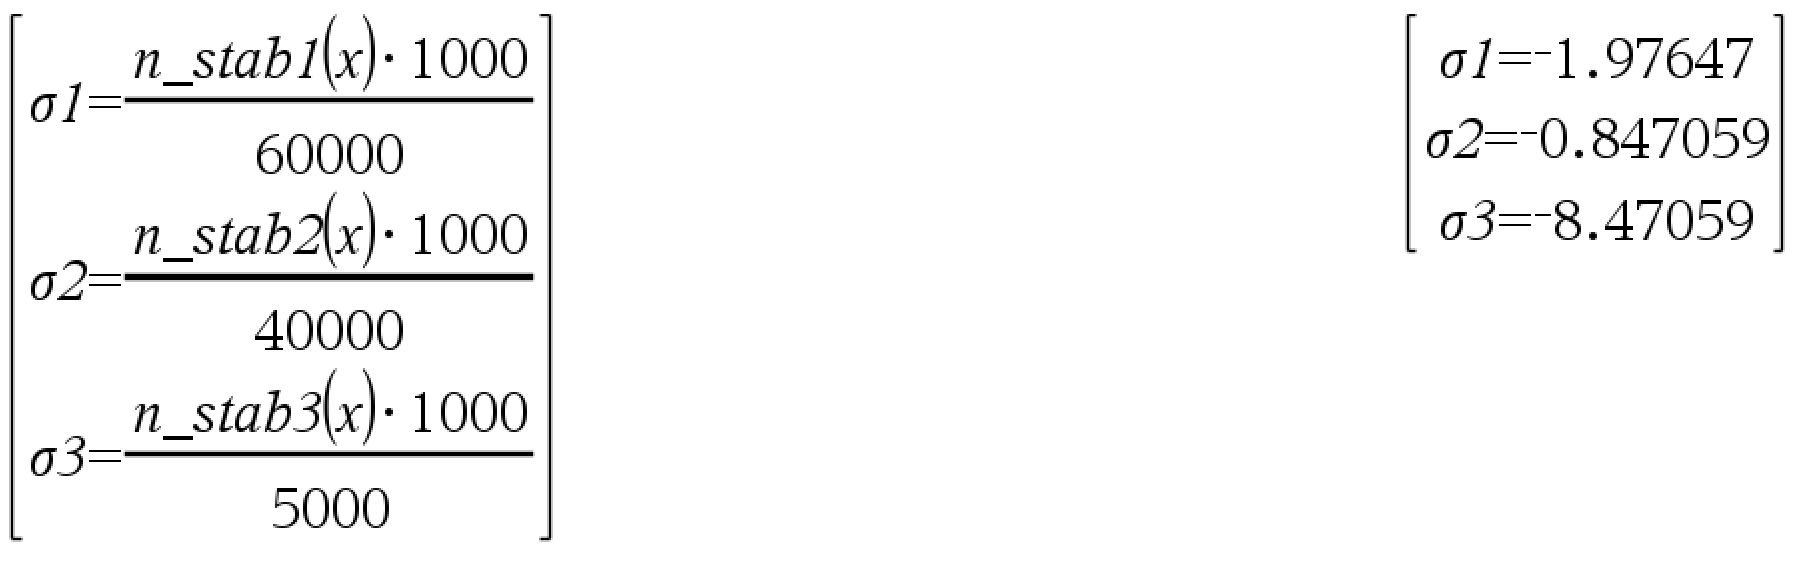
\includegraphics[width=\linewidth]{./fig/TM2/WiSe2021nr4_4.png}
        \caption{Über Schnittgrößen}
    \end{subfigure}
    \hfill
    \begin{subfigure}[t]{0.48\textwidth}
        \centering
        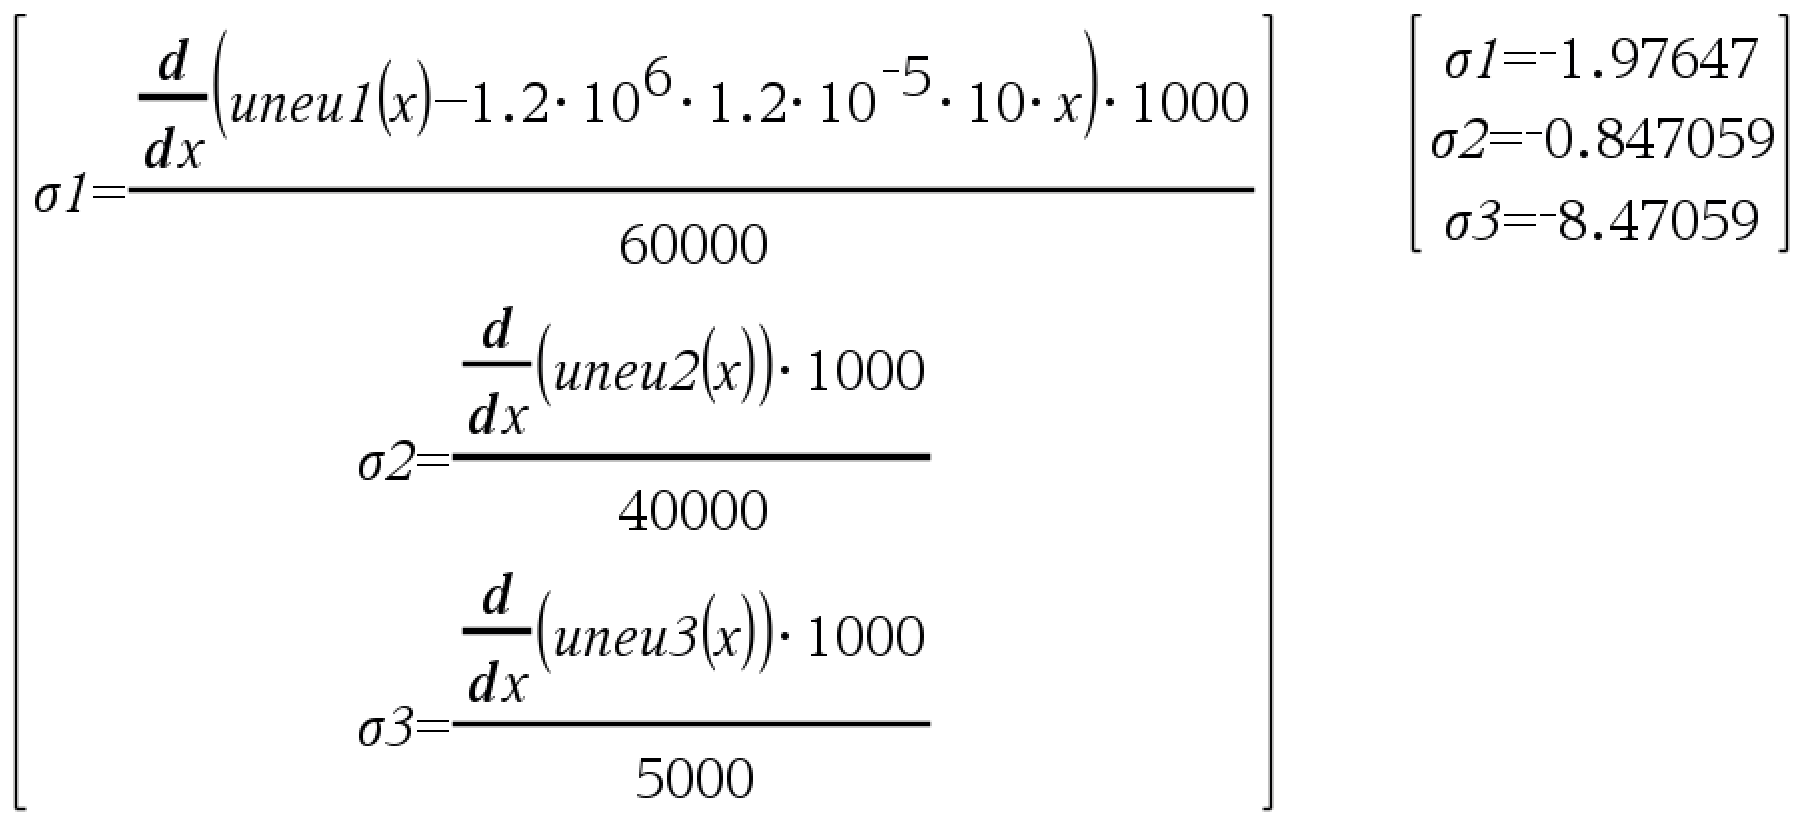
\includegraphics[width=\linewidth]{./fig/TM2/WiSe2021nr4_5.png}
        \caption{Über Verschiebungsfunktion}
    \end{subfigure}
    \caption{Lösung von TM2 WiSe~20/21, Nr.~4b}
    \label{fig:TM2WiSe2021Nr4b}
\end{figure}

Ich will hier anmerken das bei dieser Aufgabenart häufig Hinweise und Warnungen angezeigt werden. Wie z.B. hier auch bei Teilaufgabe a) eine Warnung
zur symbolischen Temperatur. Diese Warnungen sind zwar so konzipiert, dass sie nur angezeigt werden wenn das Programm bzw. ich denke
das etwas falsch eingegeben wurde, jedoch ist es schwer dabei zu vermeiden das auch bei richtiger Eingabe nie eine Warnung oder Hinweis kommt.
Aus diesem Grund empfehele ich, wenn nicht direkt ersichlich ist warum eine Warnung kommt die komplette Eingabe nochmal zu prüfen,
falls diese aber wirklicht korrekt ist sollten auch die Ergebnisse stimmen.


\subsection{Pendelstabannahme (TM2 WiSe 22/23 Nr.~4)} \label{ex:Pendelstabannahme}

\begin{figure}[htbp]
    \centering
    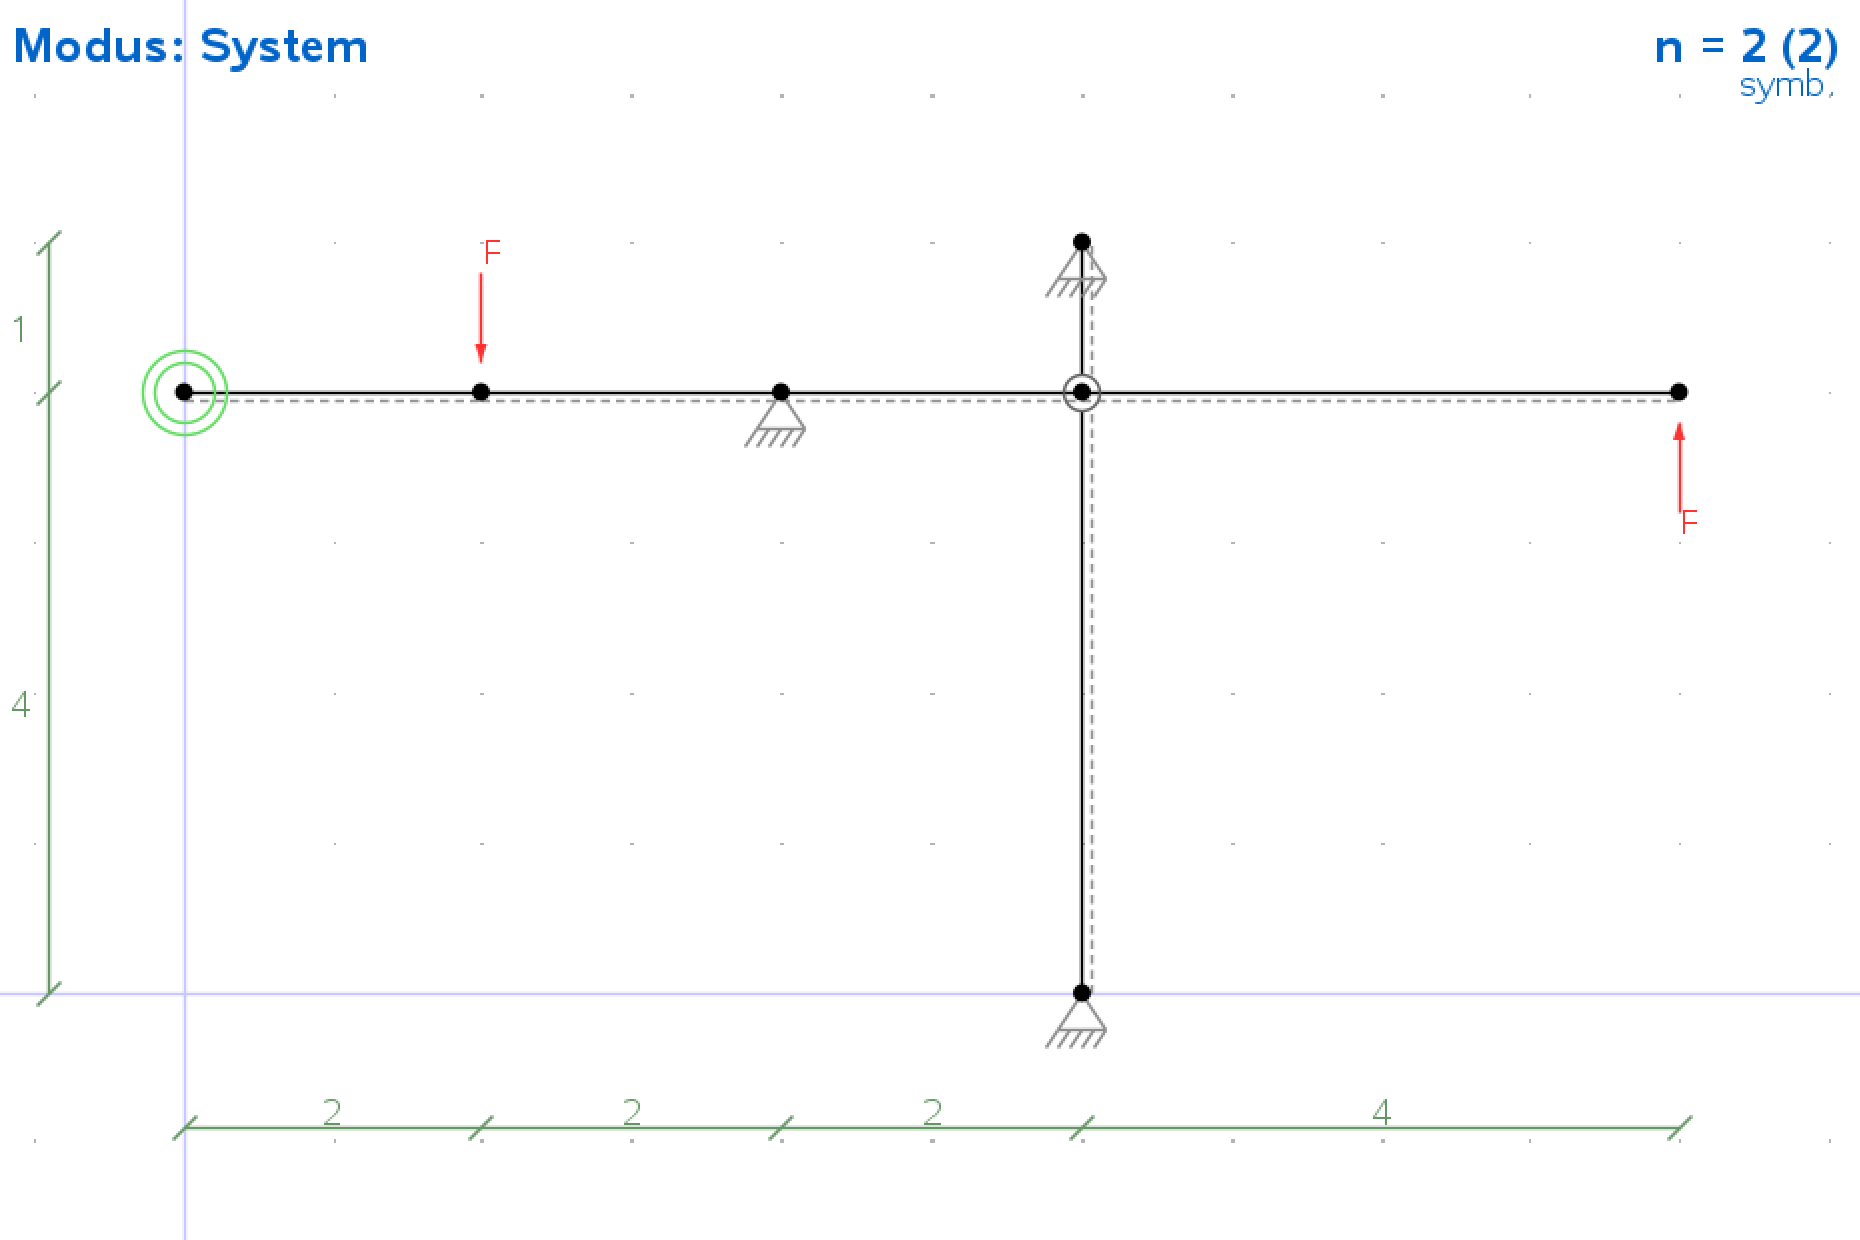
\includegraphics[width=0.7\linewidth]{./fig/TM2/WiSe2223nr4_1.png}
    \caption{TM2 WiSe~22/23, Nr.~4 im Programm}
    \label{fig:Pendelstabsnnahme}
\end{figure}

Wie die Überschrifft vielleicht bereits vermuten lässt muss bei dieser Aufgabe eine Annahme getroffen werden,
die der Zeichnung strenggenommen wiederspricht. Die beiden vertikalen stäbe sollten eigentlich mit einem Angelenk
an den starren Stab angeschlossen werden.\\
Bei einer Handrechnung wird diese Annahme quasi automatisch getroffen, das Programm macht sowas natürlich nicht automatisch.
Um diese Aufgabe mit dem Programm also korrekt zu rechnen müsseb bei den beiden vertikalen stäbe jeweils Angelenke eingebaut werden.
Falls man das nicht macht wirft das Programm eine Warnung bzw. einen Hinweis.

Bei dieser Aufgabe lassen sich die Ergebnisse entweder aus der Ansicht zur Normalkraft 
oder aus dem E-Modus holen (Abb.~\ref{fig:TM2WiSe2223Nr4}).

\begin{figure}[htbp]
    \centering
    \begin{subfigure}[t]{0.48\textwidth}
        \centering
        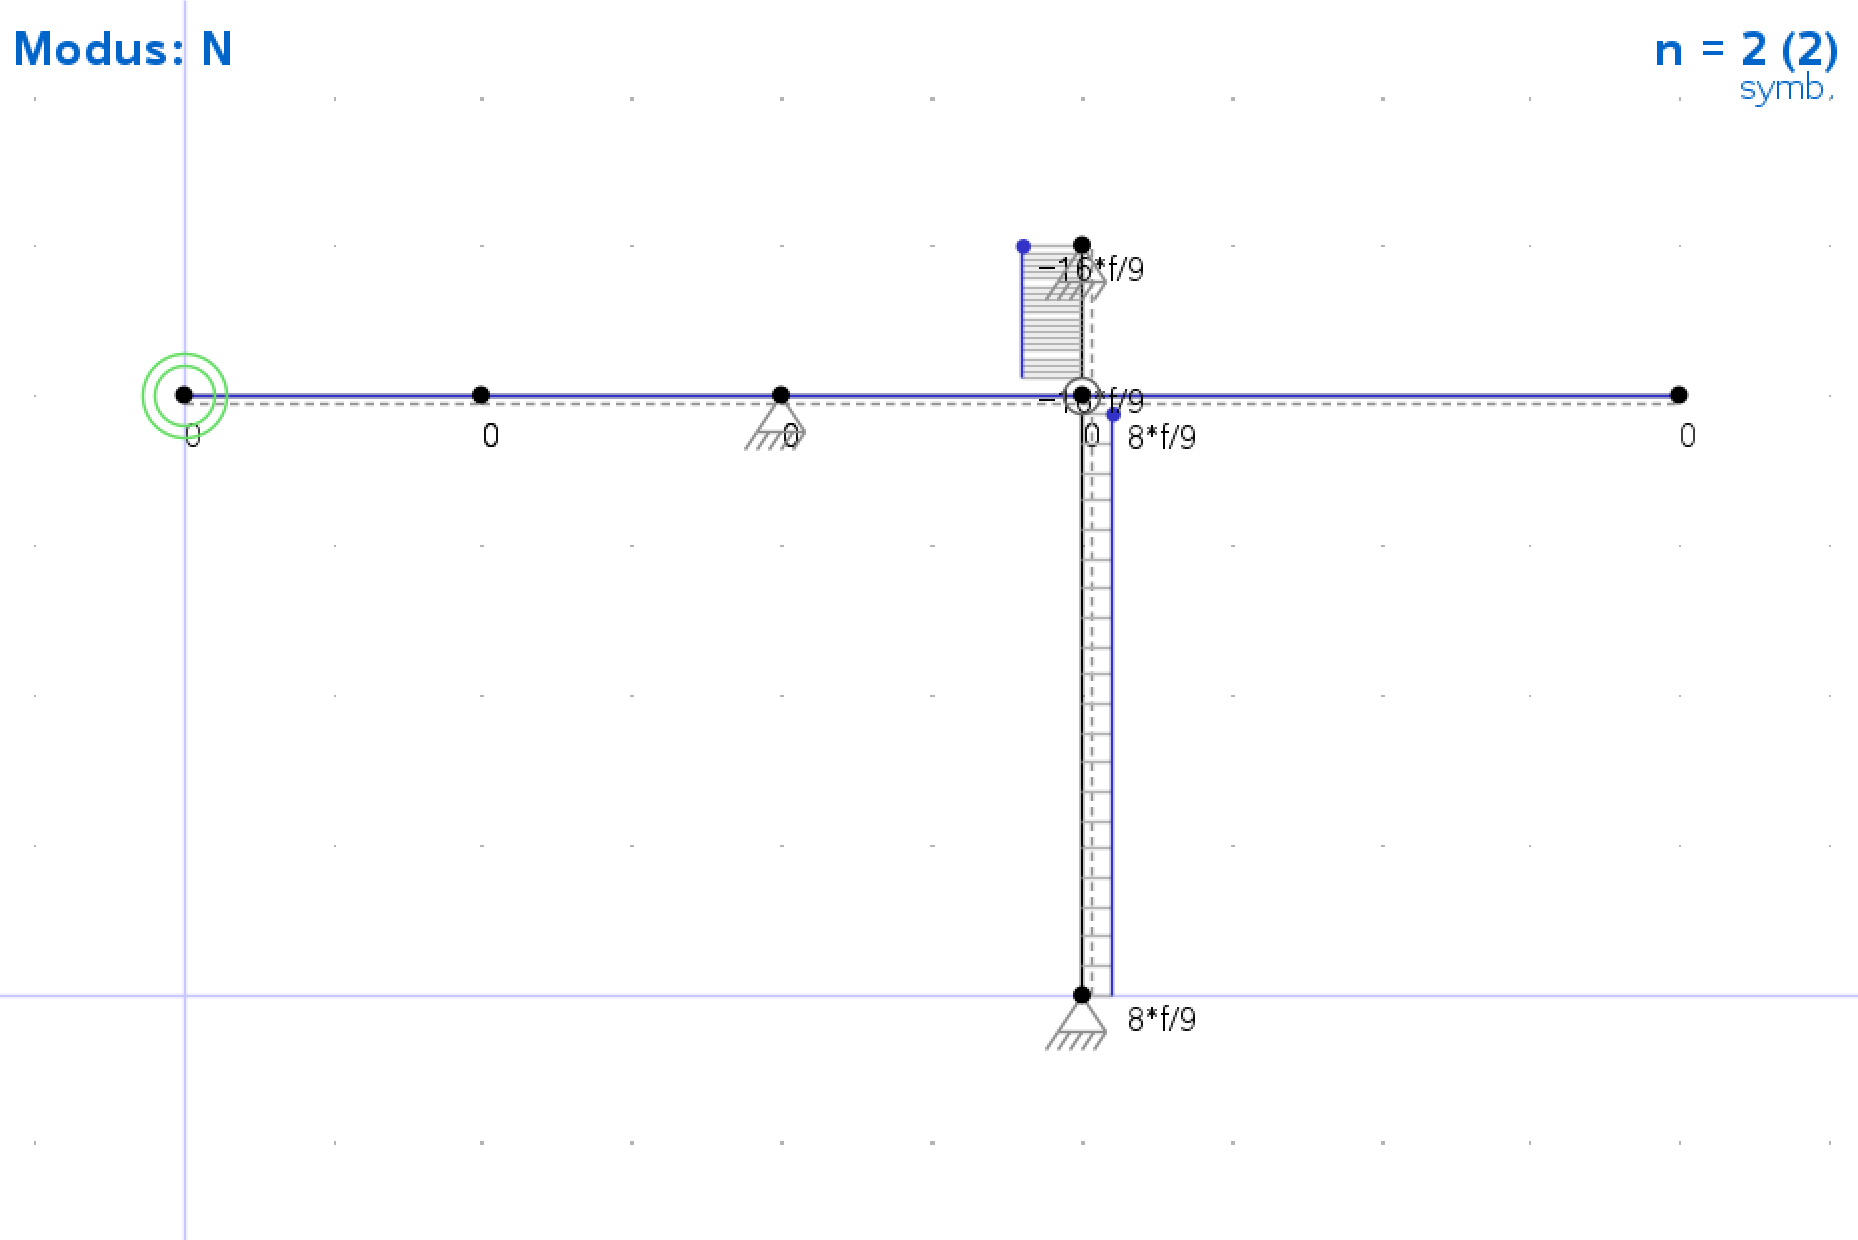
\includegraphics[width=\linewidth]{./fig/TM2/WiSe2223nr4_2.png}
        \caption{Normalkraft}
    \end{subfigure}
    \hfill
    \begin{subfigure}[t]{0.48\textwidth}
        \centering
        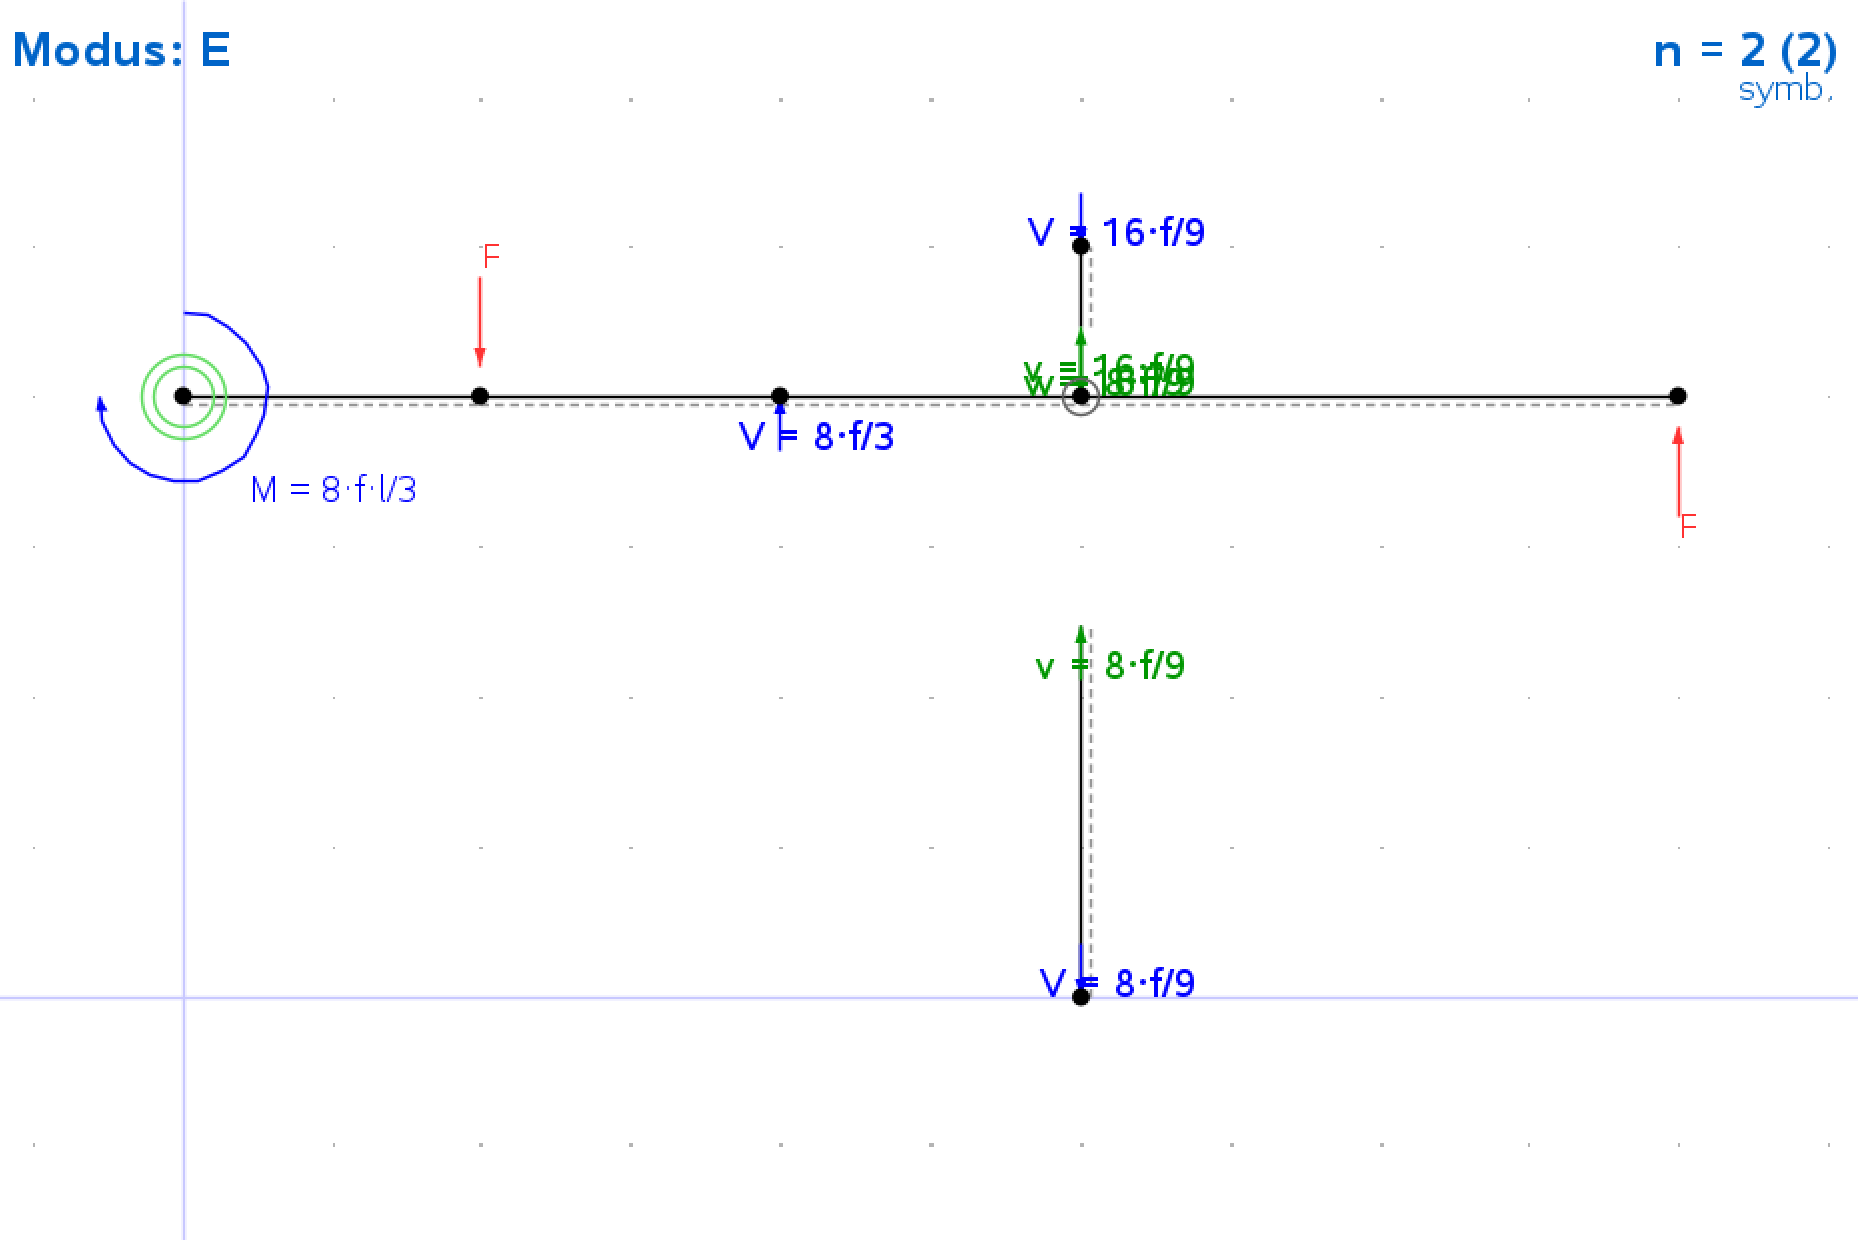
\includegraphics[width=\linewidth]{./fig/TM2/WiSe2223nr4_3.png}
        \caption{E-Modus}
    \end{subfigure}
    \caption{Lösung von TM2 WiSe~22/23, Nr.~4}
    \label{fig:TM2WiSe2223Nr4}
\end{figure}

\textbf{Wichtig} ist, dass das Programm, für symbolische Federn in den Verläufen in seltenen Fällen nicht die richtigen 
Werte ausgibt (Bei symbolischen Temperaturen sowieso nicht).
Zur Sicherheit würde ich deswegen die Schnittgrößen über die \emph{neuen} Verschiebungsfunktionen ermitteln. 
Das dauert zwar gerade für große Systeme länger, ist aber zuverlässiger weil dort wirklich alles symbolisch gerechnet wird 
und eben nicht gepfuscht wird.



\subsection{Schiefe Biegung (TM2 WiSe 25/26 Nr.~8)}

In dieser Aufgbabe sind die Dicken der dünnwandigen Elemente nicht gegeben, da diese abber sowohl für das
FTM als auch für die Lange des Schwerpunkts wichtig sind, müssen diese Werte manuell mit den Werten aus der 
Aufgabenstellung überschrieben werden. Das geht im Obermenue (Taste \taste{o}) auf Seite 3.\\
Für das Zeichnen so eines schiefen Querschnitts empfielt sich ein Rastermaß von z.B. $\frac{1}{\sqrt{2}}$.

\begin{figure}[htbp]
    \centering
    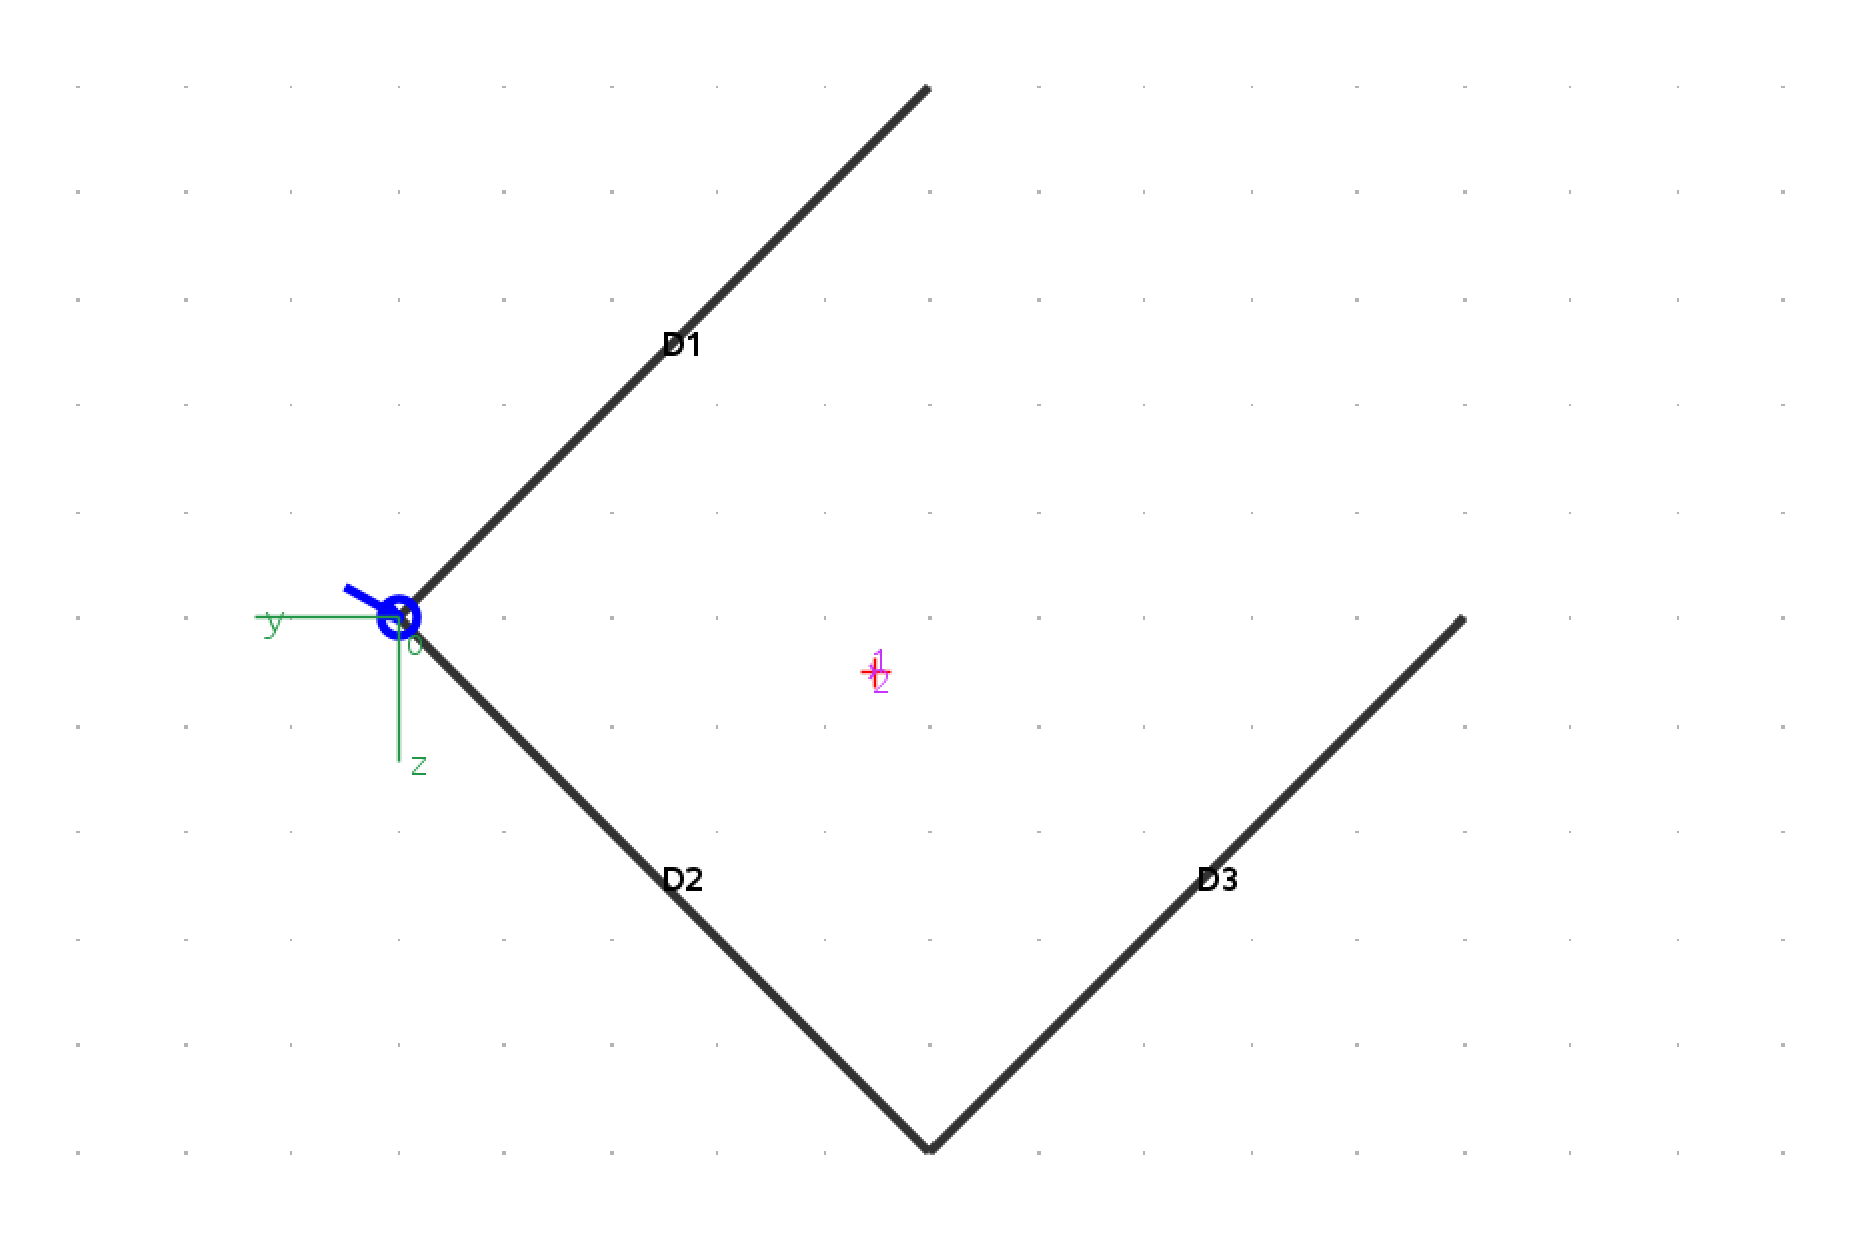
\includegraphics[width=0.7\linewidth]{./fig/TM2/WiSe2526nr8_1.png}
    \caption{TM2 WiSe~25/26, Nr.~8 im Programm}
    \label{fig:TM2WiSe2526Nr8_1}
\end{figure}

Bei dieser Aufgabe braucht man die $\sigma_x$-Berechnung. Um die Normalkraft hier richtig einzuberechnen
muss die Resultierende der Streckenlast über die halbe Länge berechnet werden, also: 
$R=0,1~\frac{\text{kN}}{cm}\cdot100~\text{cm}$.
Für die Kraft muss also $F_y=-500~\text{N}$, $F_z=300~\text{N}$ und $F_x=10000~\text{N}$ eingegeben werden.

Nach dem Aufruf der Berechnung werden noch ein paar Werte abgefragt. Für die ersten Drei muss Null eingetragen werden.
Man hätte auch keine Kraft platzieren können, die Normalkraft und Momente handisch ausrechnen können und diese dann in diese Felder eintragen können.
Das Ergebniss ist das gleiche.\\
Für $\Delta x$ muss $100~\text{cm}$ eingetragen werden, das ist der Abstand zwischen dem gezeichneten Schnitt und dem betrachteten Schnitt.
Das Programm rechnet dann also automatisch die Momente aus der Querkraft aus. Dieses Feature funktioniert natürlich nur, wenn zwischen dem gezeichneten und berechneten Schnitt
keine Weiteren Einflüsse wie Lager oder Kräfte Angreiffen, dann kommt man nicht darum herum $N$, $M_y$ und $M_z$ händisch auszurechnen und einzutragen.

Die Ergebnisse sind in Abbildung \ref{fig:TM2WiSe2526Nr8_2} dargestellt.

\begin{figure}[htbp]
    \centering
    \begin{subfigure}[t]{0.48\textwidth}
        \centering
        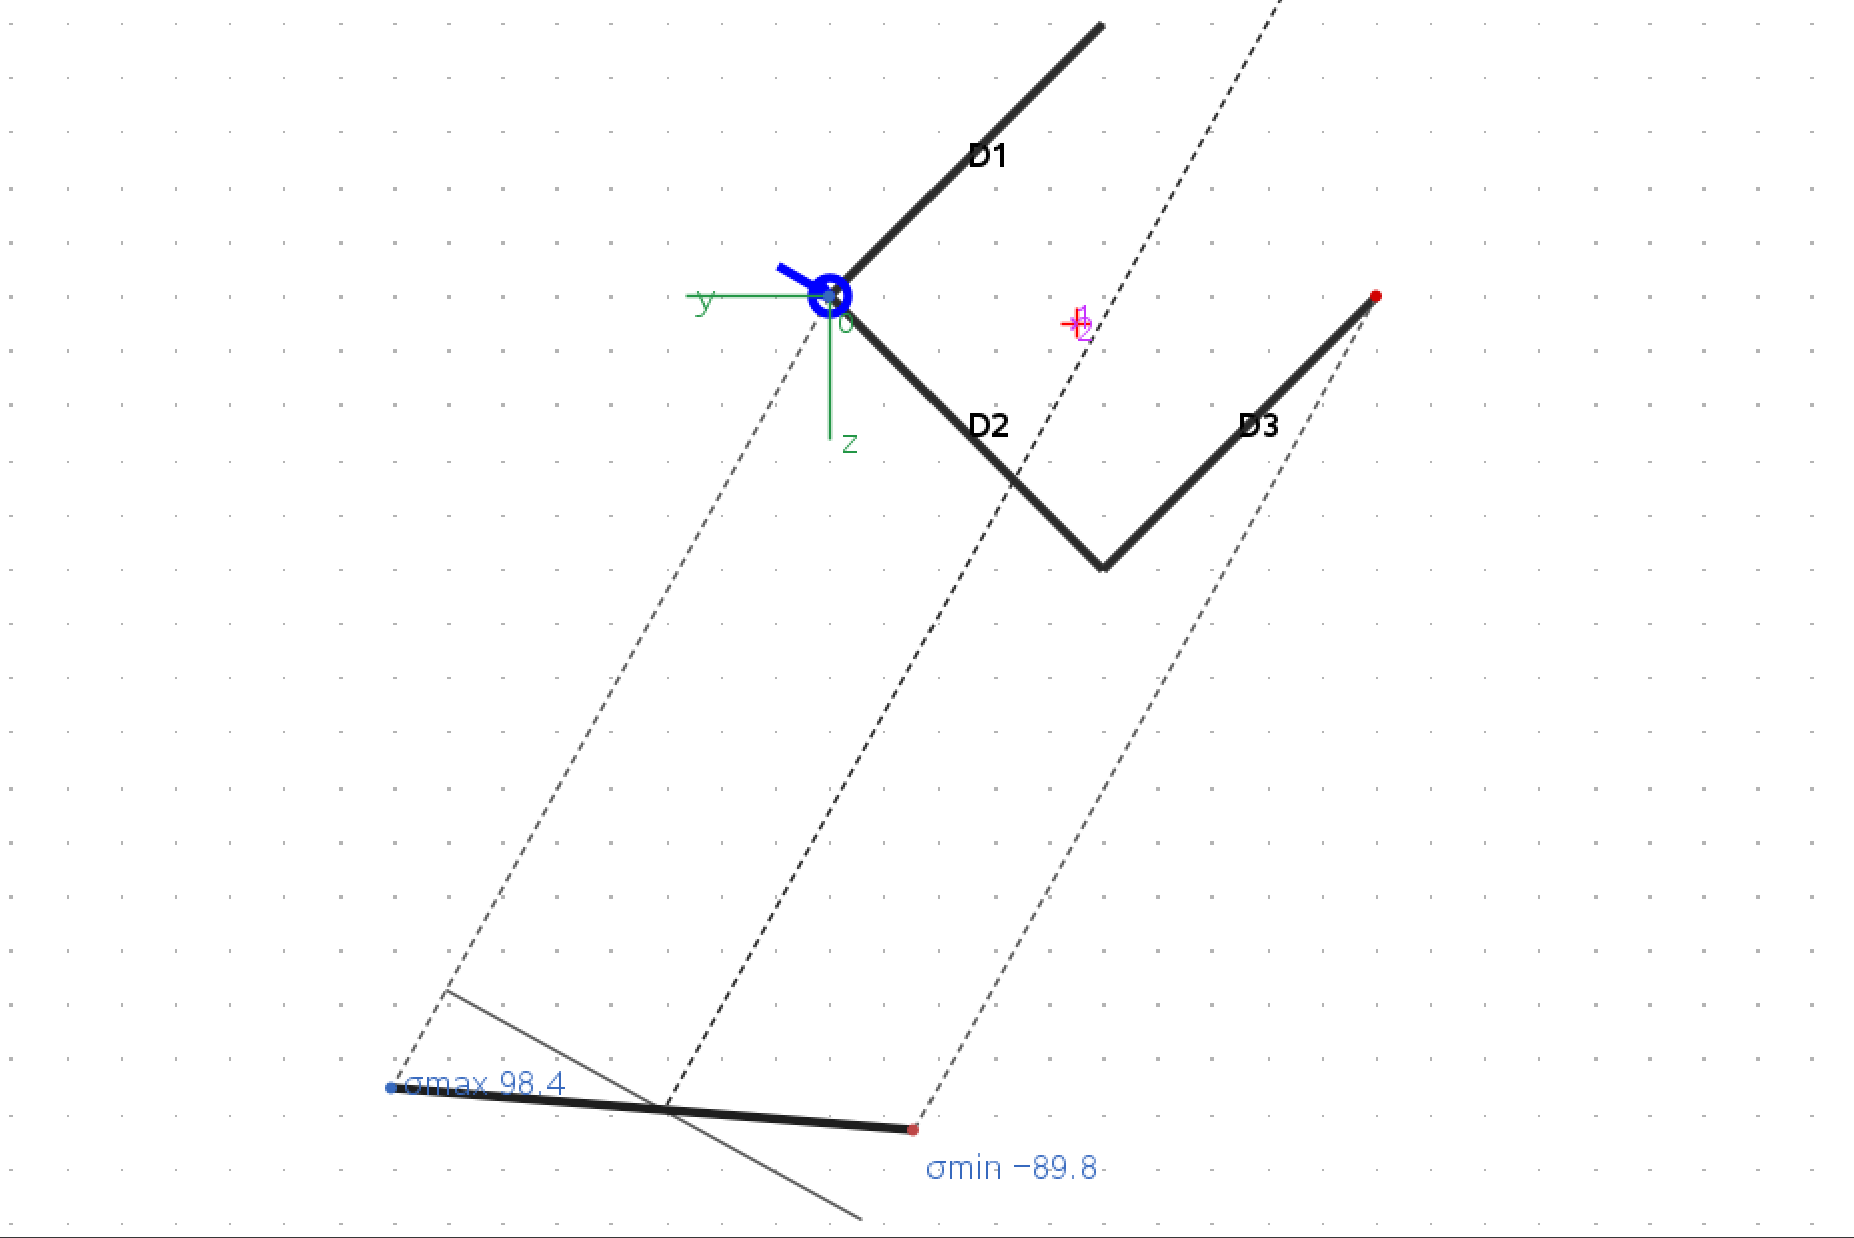
\includegraphics[width=\linewidth]{./fig/TM2/WiSe2526nr8_2.png}
        \caption{Spannungsverlauf}
    \end{subfigure}
    \hfill
    \begin{subfigure}[t]{0.48\textwidth}
        \centering
        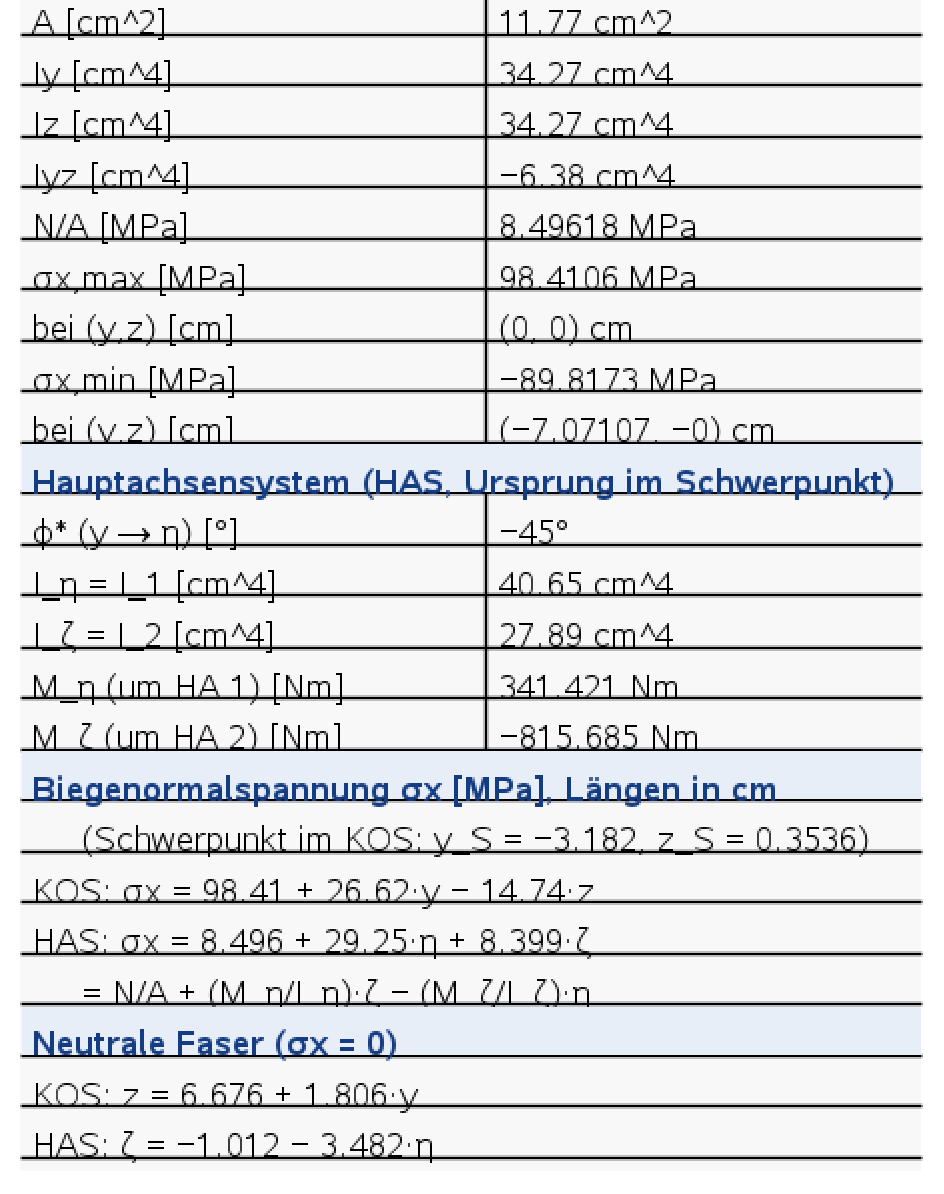
\includegraphics[width=\linewidth]{./fig/TM2/WiSe2526nr8_3.png}
        \caption{Tabellen übersicht}
    \end{subfigure}
    \caption{Lösung von TM2 WiSe~25/26, Nr.~8}
    \label{fig:TM2WiSe2526Nr8_2}
\end{figure}

Ich will anmereken, dass des öfteren bei Aufgaben Querschnittswerte gegeben sind, die nicht zur Bemaßung in der Zeichnung passen,
ob das absichtlich so ist konnte mir leider keiner sagen. Es ist also immer sinnvoll das einmal gegen zu prüfen und die Werte evtl. zu überschreiben.
Was die ISD-Musterlösung bei dieser Aufgabe gerechnet hat, ist mir nicht ganz klar. Meines Verständnisses nach wurde hier mit einem
Schwerpunkt für die Momente aus Normalkraft gerechnet, der genau in der Mitte des U profiels liegt, sodass die Normalkraft um die $y$-Achse kein Moment erzeugt.

\subsection{Schiefe Biegung/Kernfäche (TM2 WiSe21/22 Nr.~8)}



\subsection{MSK (TM2 WiSe 21/22 Nr.~3)}

Zu dieser Aufgabe gibt es eigentlich nicht besonders viel zu sagen, man gibt die gegebenen Werte ein und das Programm
füllt in grün die restlichen Werte auf (Abb.~\ref{fig:TM2WiSe2122Nr3_1}).

\begin{figure}[htbp]
    \centering
    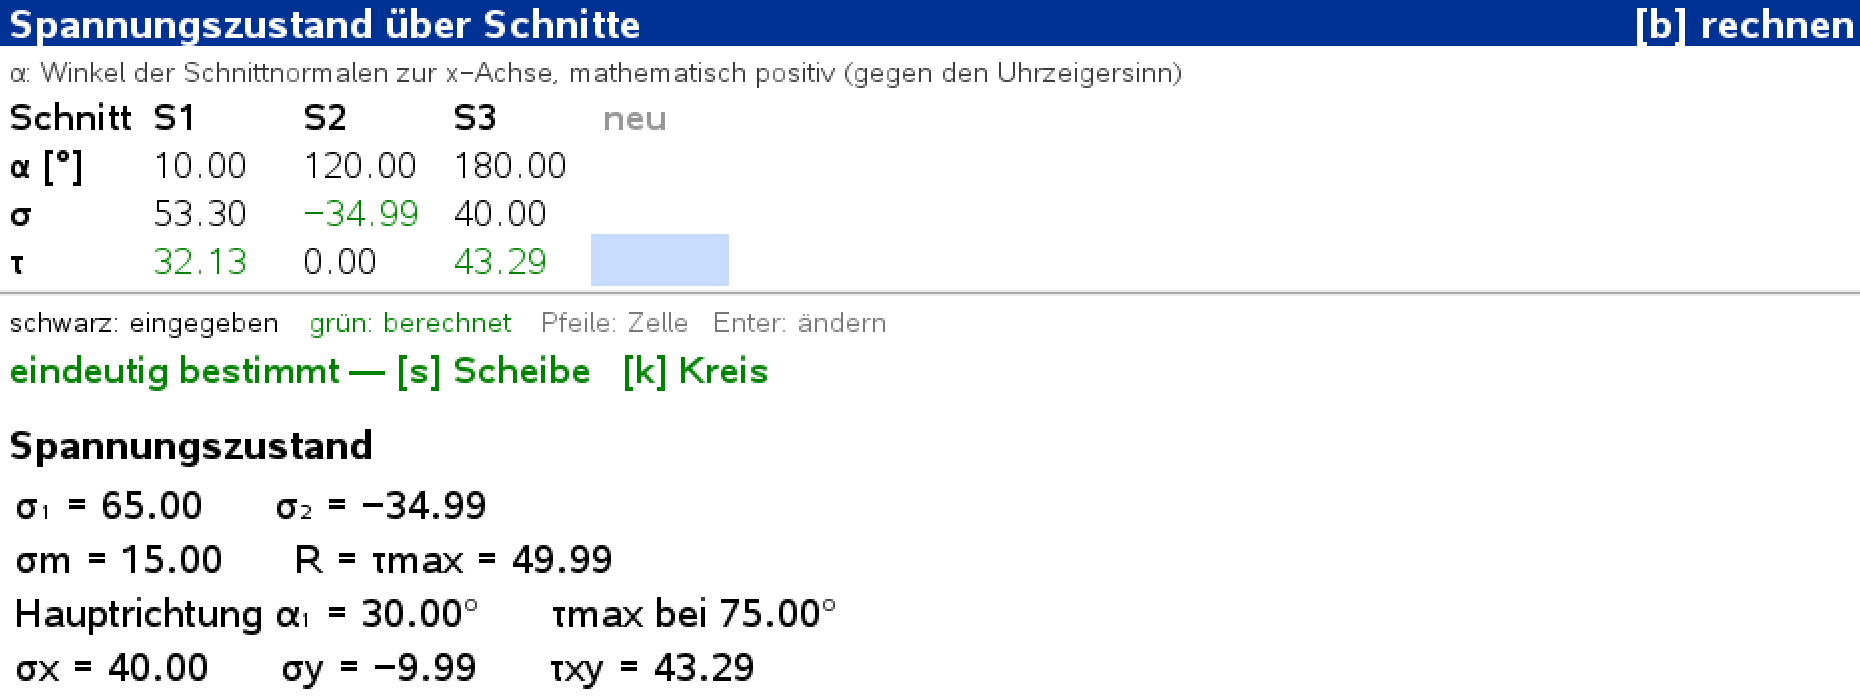
\includegraphics[width=0.7\linewidth]{./fig/TM2/WiSe2122nr3_1.png}
    \caption{TM2 WiSe~21/22, Nr.~3 im Programm}
    \label{fig:TM2WiSe2122Nr3_1}
\end{figure}

Danach bekommt man mit den Tasten \taste{s} und \taste{k} die beiden wichtigen Ansichten (Abb.~\ref{fig:TM2WiSe2122Nr3_2}).


\begin{figure}[htbp]
    \centering
    \begin{subfigure}[t]{0.48\textwidth}
        \centering
        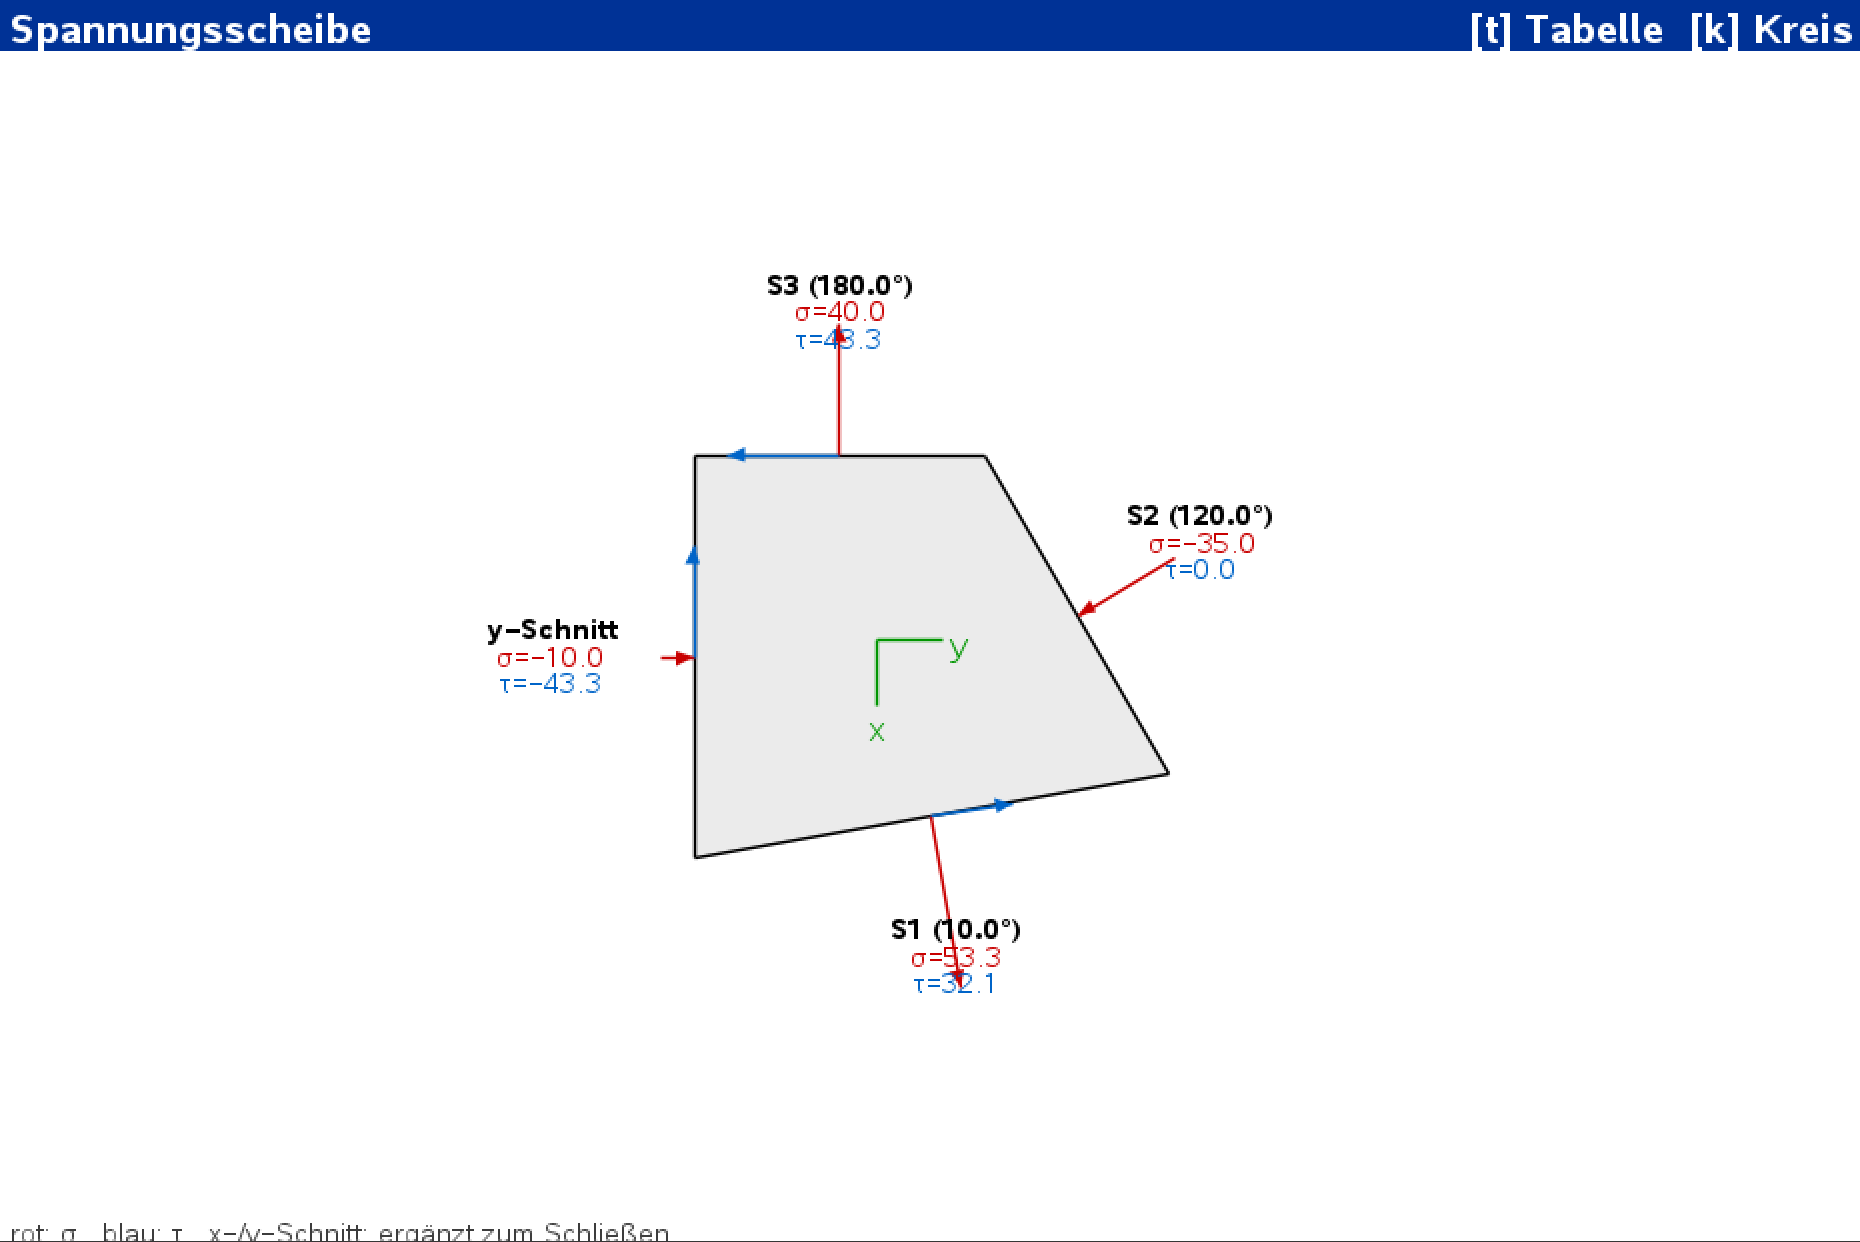
\includegraphics[width=\linewidth]{./fig/TM2/WiSe2122nr3_2.png}
        \caption{Spannungs-Scheibe}
    \end{subfigure}
    \hfill
    \begin{subfigure}[t]{0.48\textwidth}
        \centering
        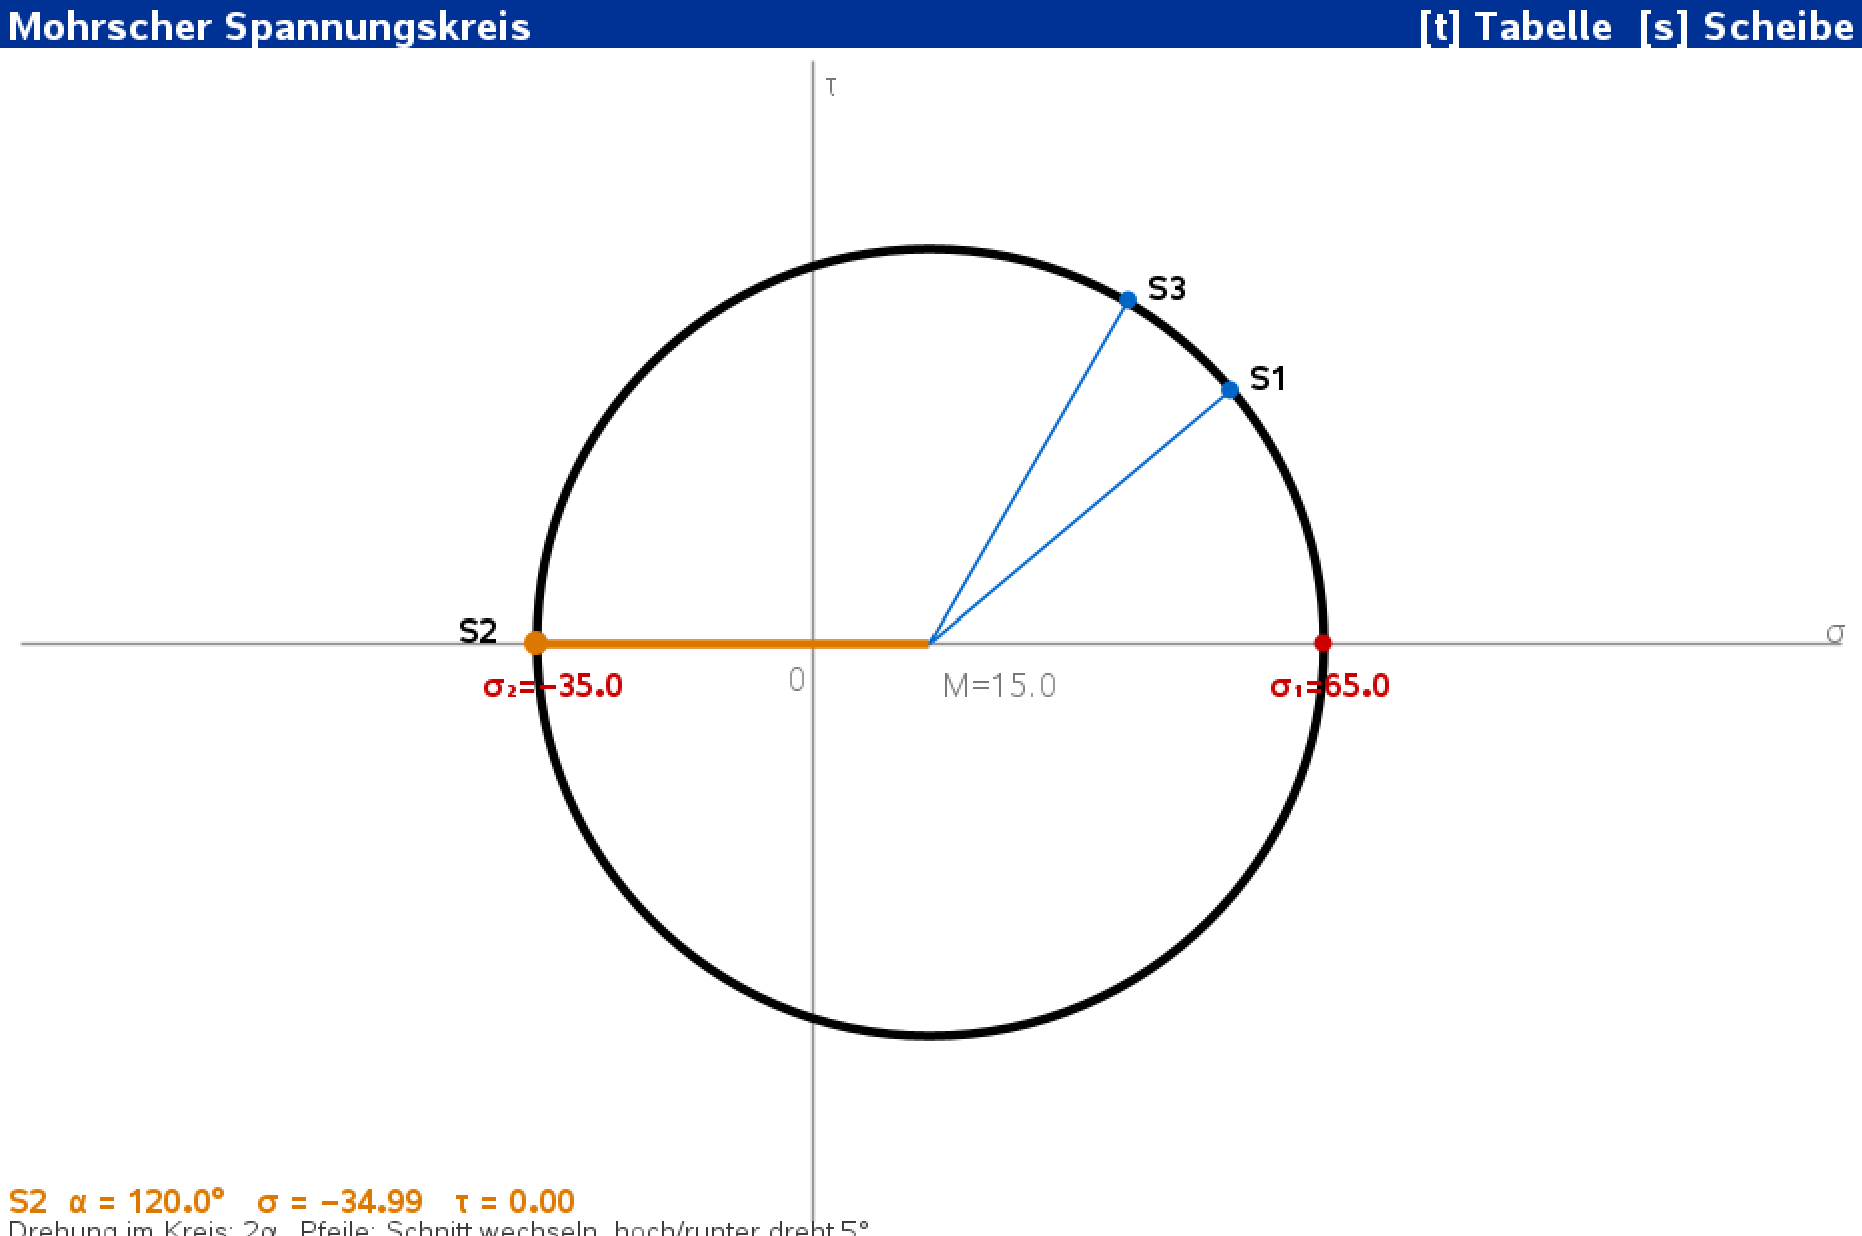
\includegraphics[width=\linewidth]{./fig/TM2/WiSe2122nr3_3.png}
        \caption{Spannungs-Kreis}
    \end{subfigure}
    \caption{Lösung von TM2 WiSe~21/22, Nr.~3}
    \label{fig:TM2WiSe2122Nr3_2}
\end{figure}

Falls bei einer Aufgabe nach dem Winkel eines Schnitts gefragt wird und das Programm zwei Winkel ausgibt, muss natürlich
geprüft werden, welcher Winkel eher zur Skizze passt.

\subsection{Schubspannung und SMP (TM2 SoSe 24 Nr.~8)}

\subsection{Verwölbung (TM2 SoSe 20 Nr.~9)} eingebunden.
% Hier keine \usepackage-Zeilen: Pakete stehen in der Praeambel von Anleitung.tex.
% Abbildungen mit [htbp]: LaTeX setzt sie dann dorthin, wo Platz ist. Im Text deshalb immer
% mit Abb.~\ref{...} auf sie verweisen, nicht mit "unten" oder "folgendermaßen".


\part{Beispiele}

In diesem Teil will ich anhand typischer Klausuraufgaben etwas genauer beschreiben, wie man das
Programm am besten verwendet, zumindest so, wie ich es für sinnvoll halte.

Die Screenshots habe ich in der PC-Ansicht gemacht, weil dort viele Dinge besser erkennbar sind.
Auf dem Taschenrechner selbst sollte mit Zoom aber auch alles erkennbar sein.

\section{TM1}
\subsection{WiSe~21/22}
\subsubsection{Geschlossenes System (Nr.~2)}
Bei dieser Aufgabe gibt es ein paar Besonderheiten bei der Eingabe, deshalb stelle ich sie hier vor.
Im Programm sieht das Tragwerk aus wie in Abb.~\ref{fig:WiSe2122nr2_1}.

\begin{figure}[htbp]
    \centering
    \begin{subfigure}[t]{0.48\textwidth}
        \centering
        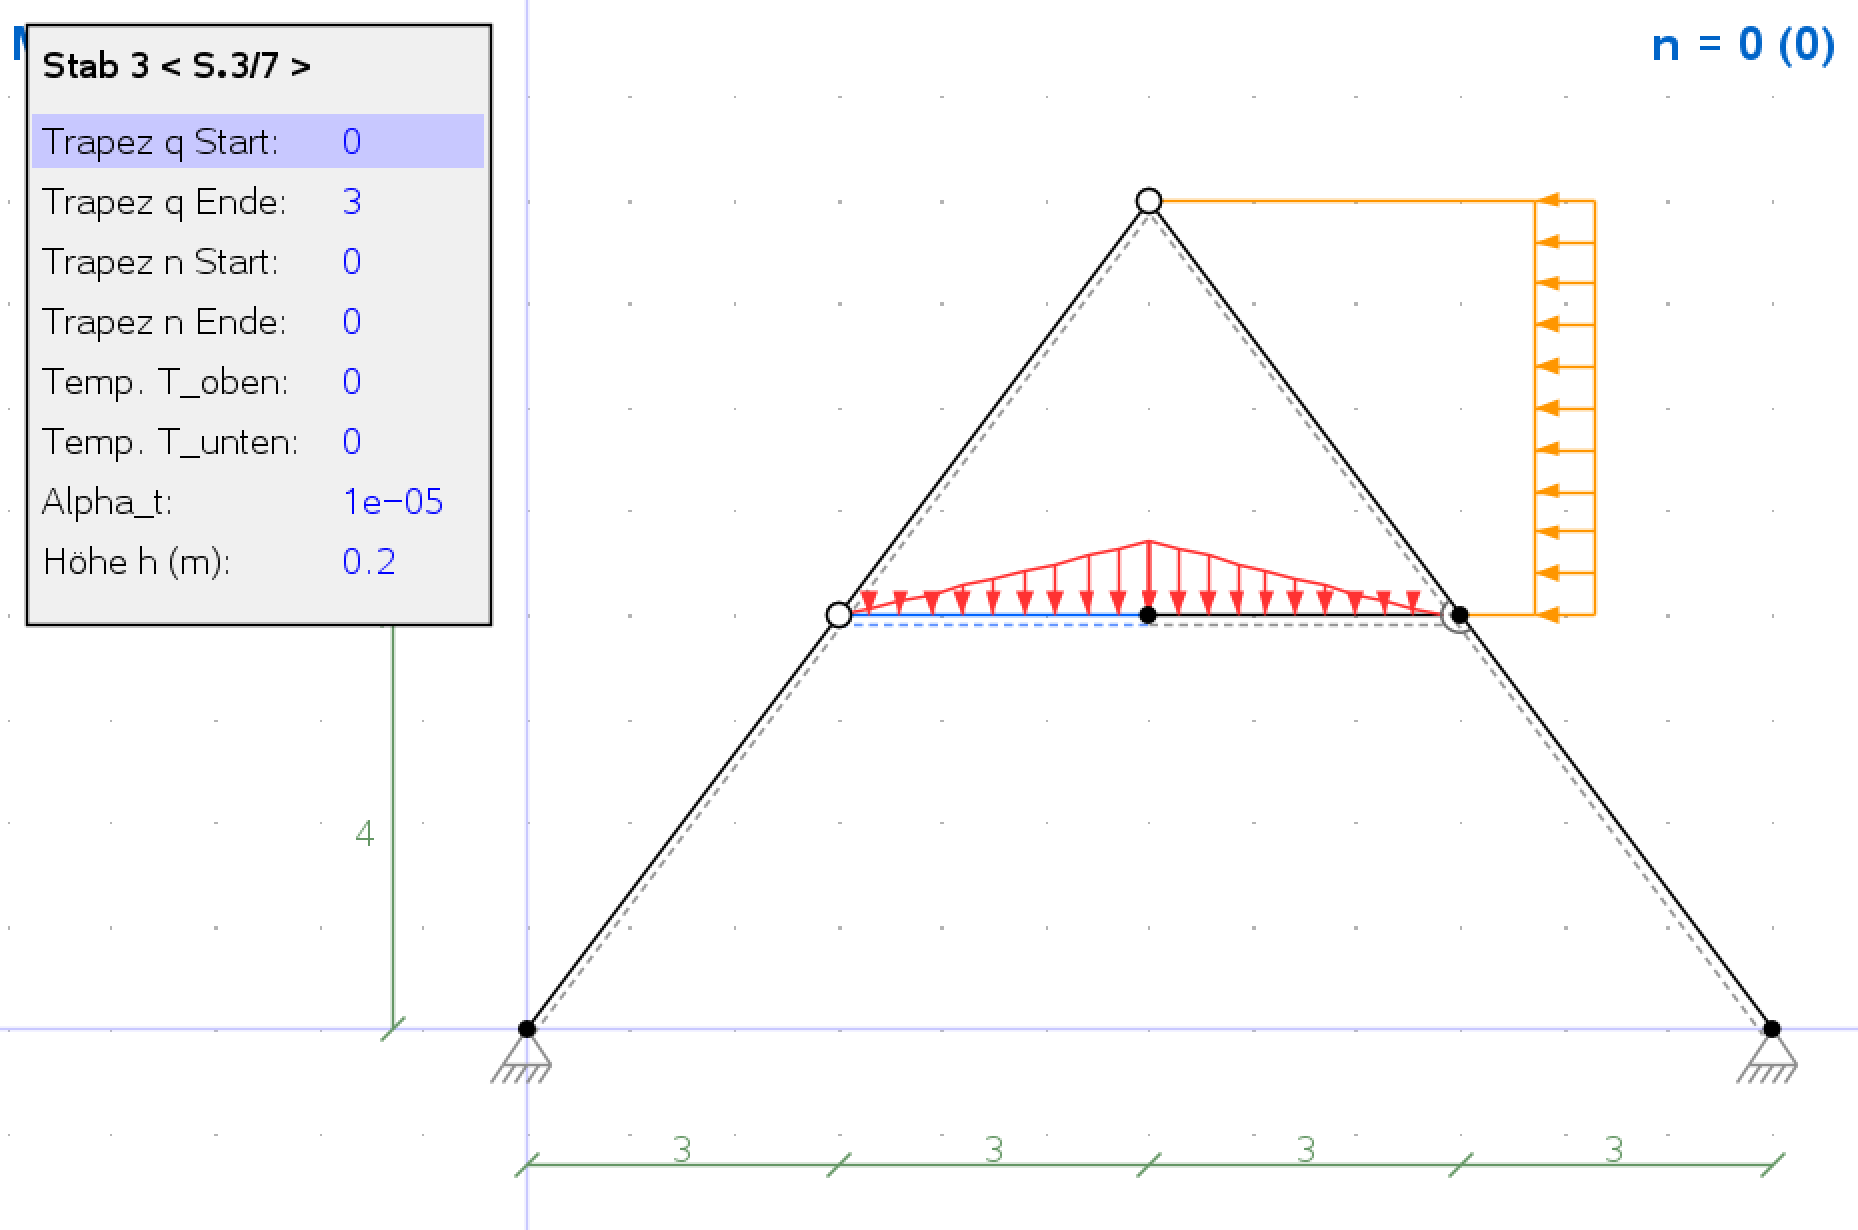
\includegraphics[width=\linewidth]{./fig/TM1/WiSe2122nr2_1.png}
        \caption{Trapezlast auf der linken Hälfte des Mittelstabs}
    \end{subfigure}
    \hfill
    \begin{subfigure}[t]{0.48\textwidth}
        \centering
        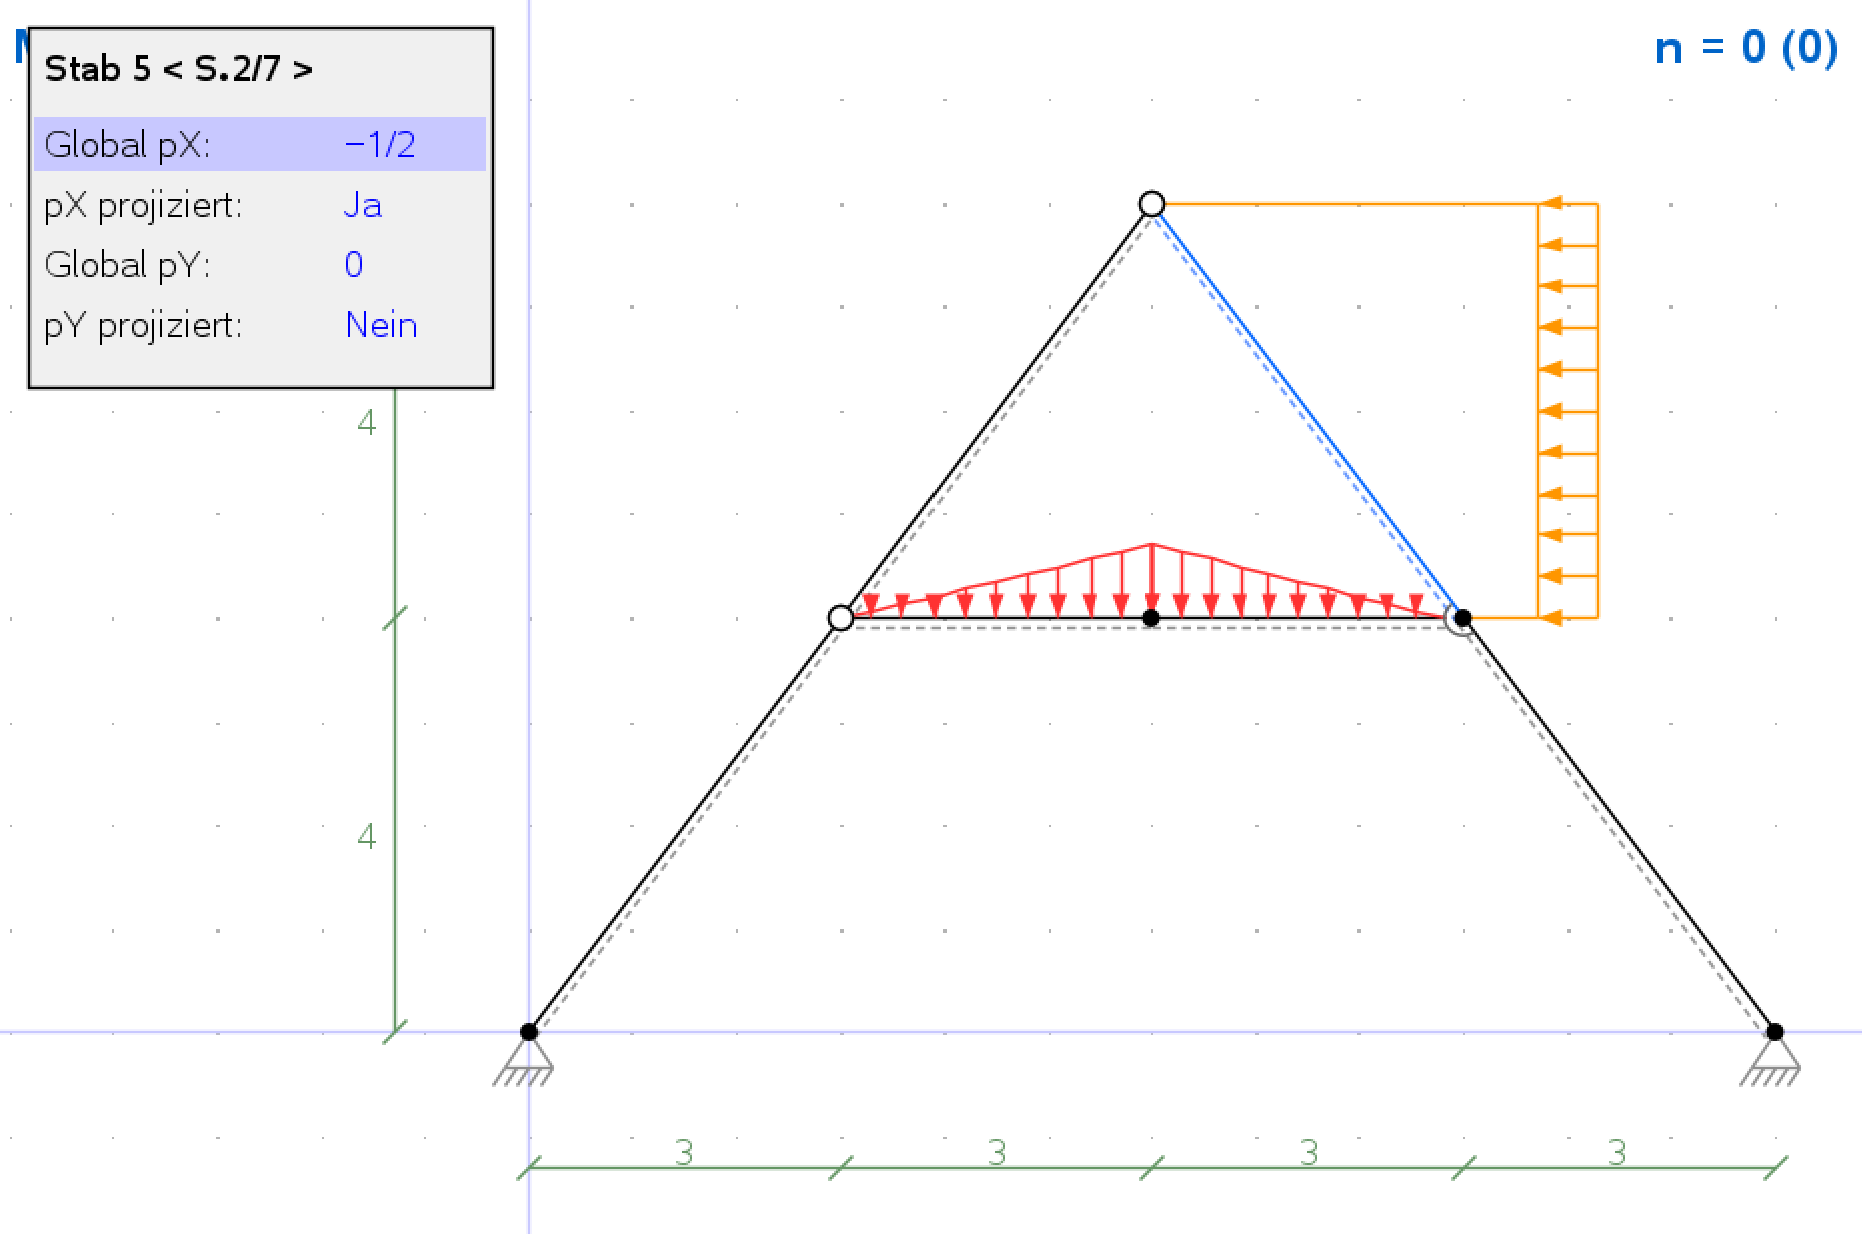
\includegraphics[width=\linewidth]{./fig/TM1/WiSe2122nr2_2.png}
        \caption{globale Streckenlast am oberen rechten Stab}
    \end{subfigure}
    \caption{WiSe~21/22, Nr.~2 im Programm}
    \label{fig:WiSe2122nr2_1}
\end{figure}

Den Stab in der Mitte müsst ihr im Programm teilen. Die Last auf ihm ist dreieckförmig mit der
Spitze in der Mitte, eine Trapezlast geht aber immer über einen ganzen Stab. Jede Hälfte bekommt
deshalb ihre eigene Trapezlast, die linke von $0$ auf $3$, die rechte von $3$ auf $0$
(Abb.~\ref{fig:WiSe2122nr2_1}a). Der neue Knoten in der Mitte bleibt biegesteif.

Die Streckenlast am schrägen Stab gebt ihr am einfachsten als globale Last ein
(Abb.~\ref{fig:WiSe2122nr2_1}b). In der Aufgabe ist sie auf die senkrechte Projektion des Stabes
bezogen, deshalb muss \emph{pX projiziert} auf \emph{Ja} stehen. Negativ ist sie, weil sie global
gesehen entgegen der $x$-Achse wirkt, also nach links.

Nach dem Berechnen könnt ihr das LGS, das zur Explosionsansicht (Abb.~\ref{fig:WiSe2122nr2_2})
gehört, über die zweite Seite des Obermenüs (\emph{LGS-Matrix}) in den Taschenrechner exportieren
(Abb.~\ref{fig:WiSe2122nr2_3}). Die Gleichungen stehen dann lesbar in \code{lgs}, die Lösung
bekommt ihr zum Beispiel mit \code{ggw\_x = ggw\_a$^{-1}$*ggw\_b}
(Abschnitt~\ref{sec:lgs-matrix}).

\begin{figure}[htbp]
    \centering
    \begin{subfigure}[t]{0.48\textwidth}
        \centering
        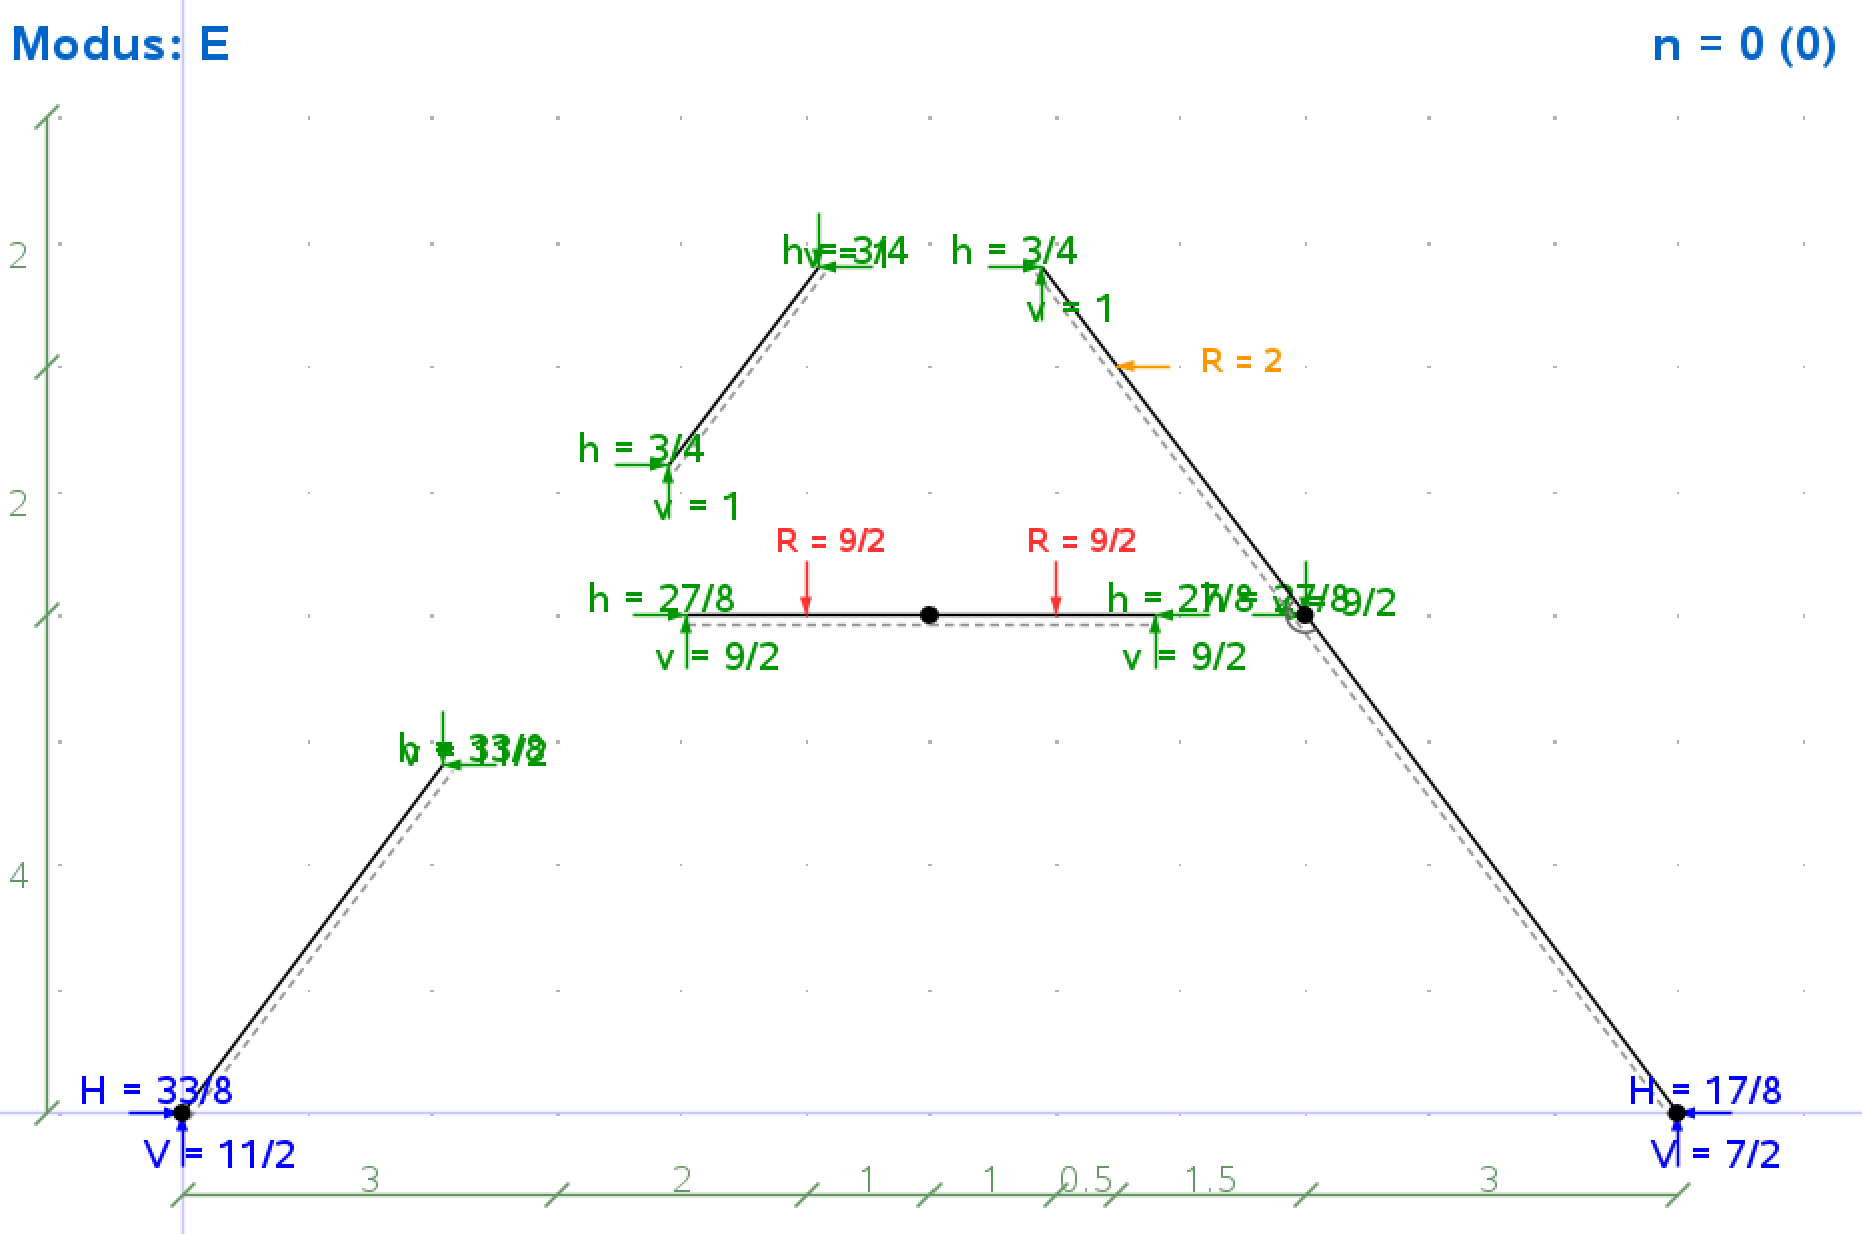
\includegraphics[width=\linewidth]{./fig/TM1/WiSe2122nr2_5.png}
        \caption{Seite~1: Ergebnisse in ihrer wirklichen Richtung}
    \end{subfigure}
    \hfill
    \begin{subfigure}[t]{0.48\textwidth}
        \centering
        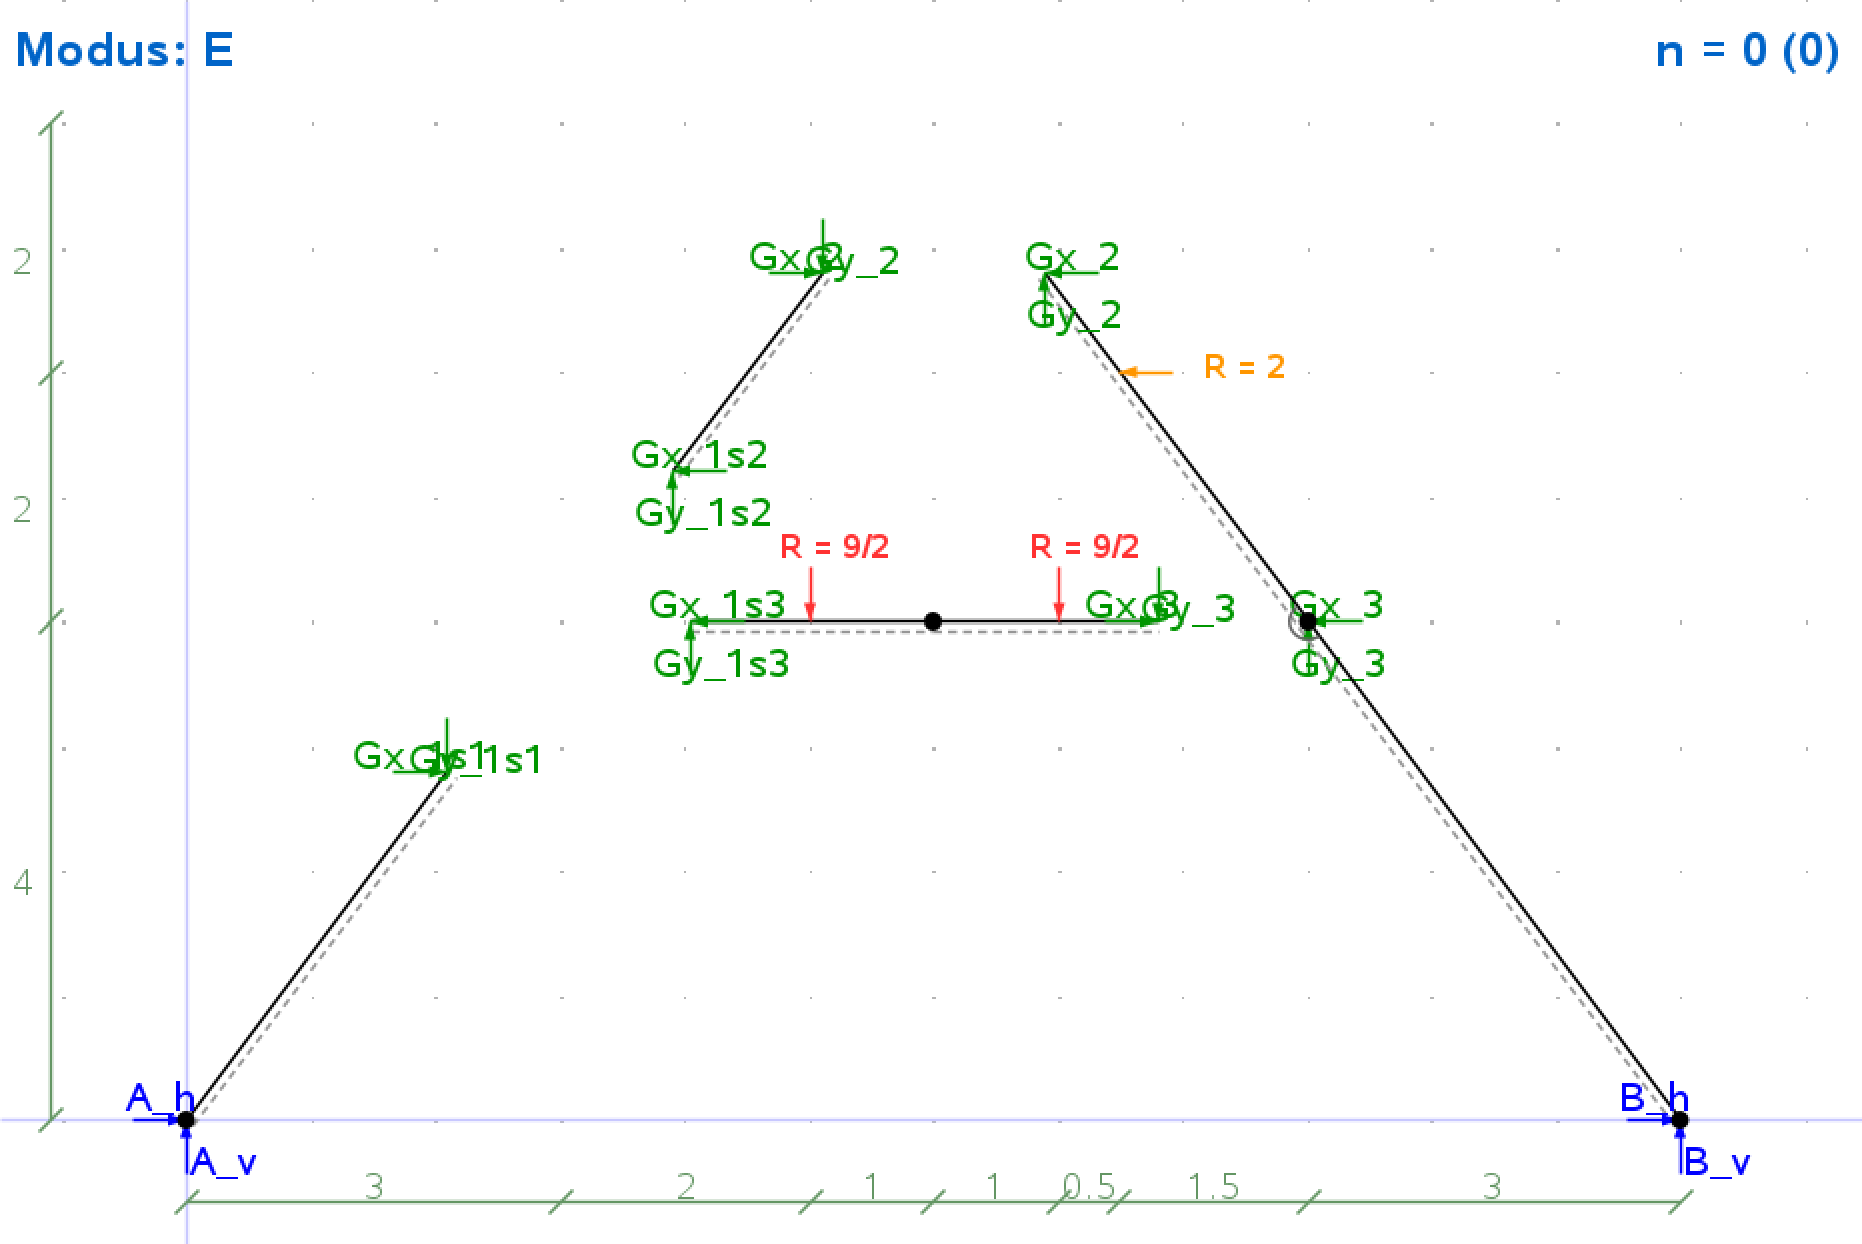
\includegraphics[width=\linewidth]{./fig/TM1/WiSe2122nr2_6.png}
        \caption{Seite~2: Unbekannte in positiver Richtung}
    \end{subfigure}
    \caption{WiSe~21/22, Nr.~2: Explosionsansicht (E-Modus)}
    \label{fig:WiSe2122nr2_2}
\end{figure}

\begin{figure}[htbp]
    \centering
    \begin{subfigure}[t]{0.48\textwidth}
        \centering
        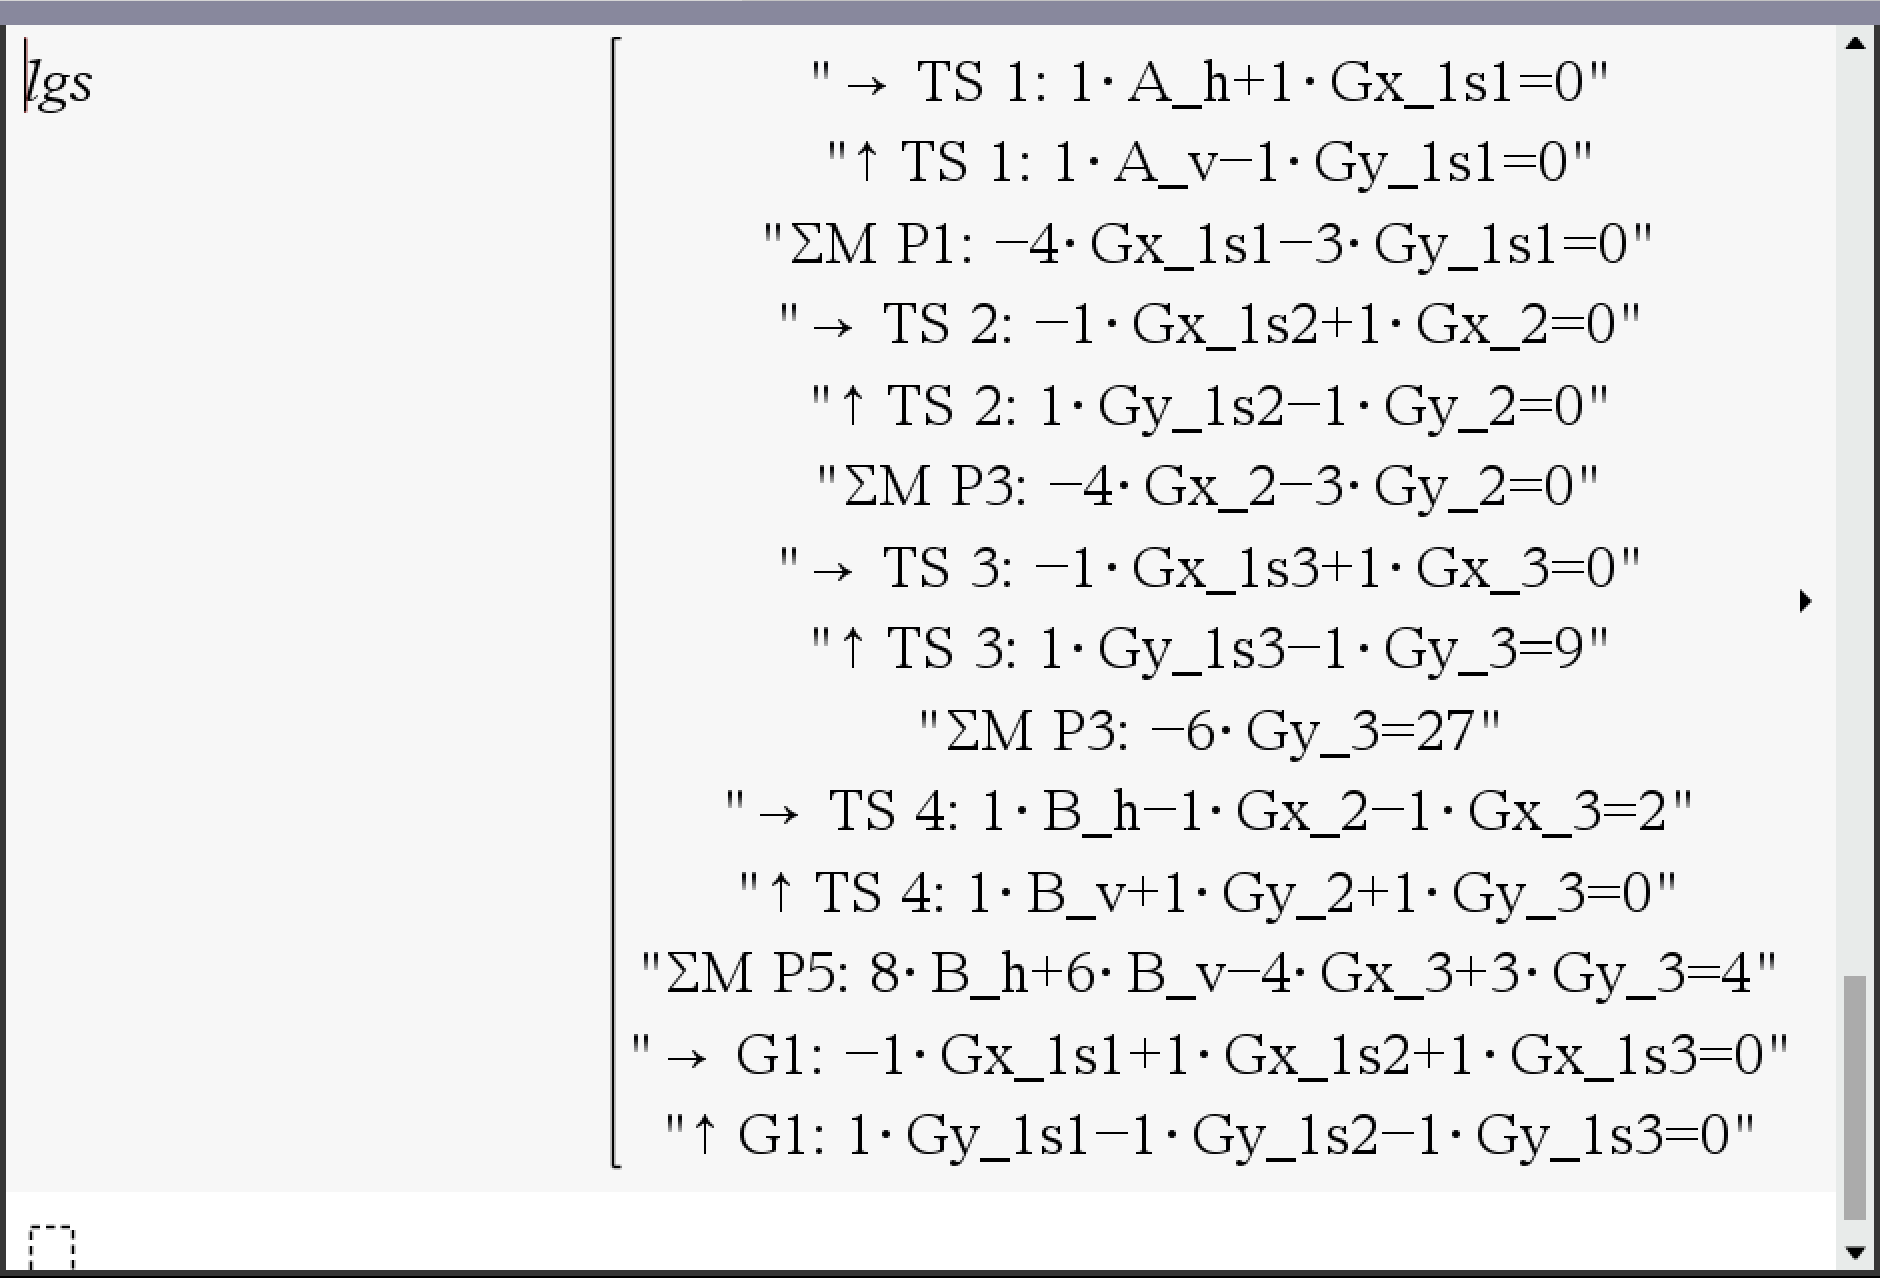
\includegraphics[width=\linewidth]{./fig/TM1/WiSe2122nr2_3.png}
        \caption{exportierte Gleichungen \code{lgs}}
    \end{subfigure}
    \hfill
    \begin{subfigure}[t]{0.48\textwidth}
        \centering
        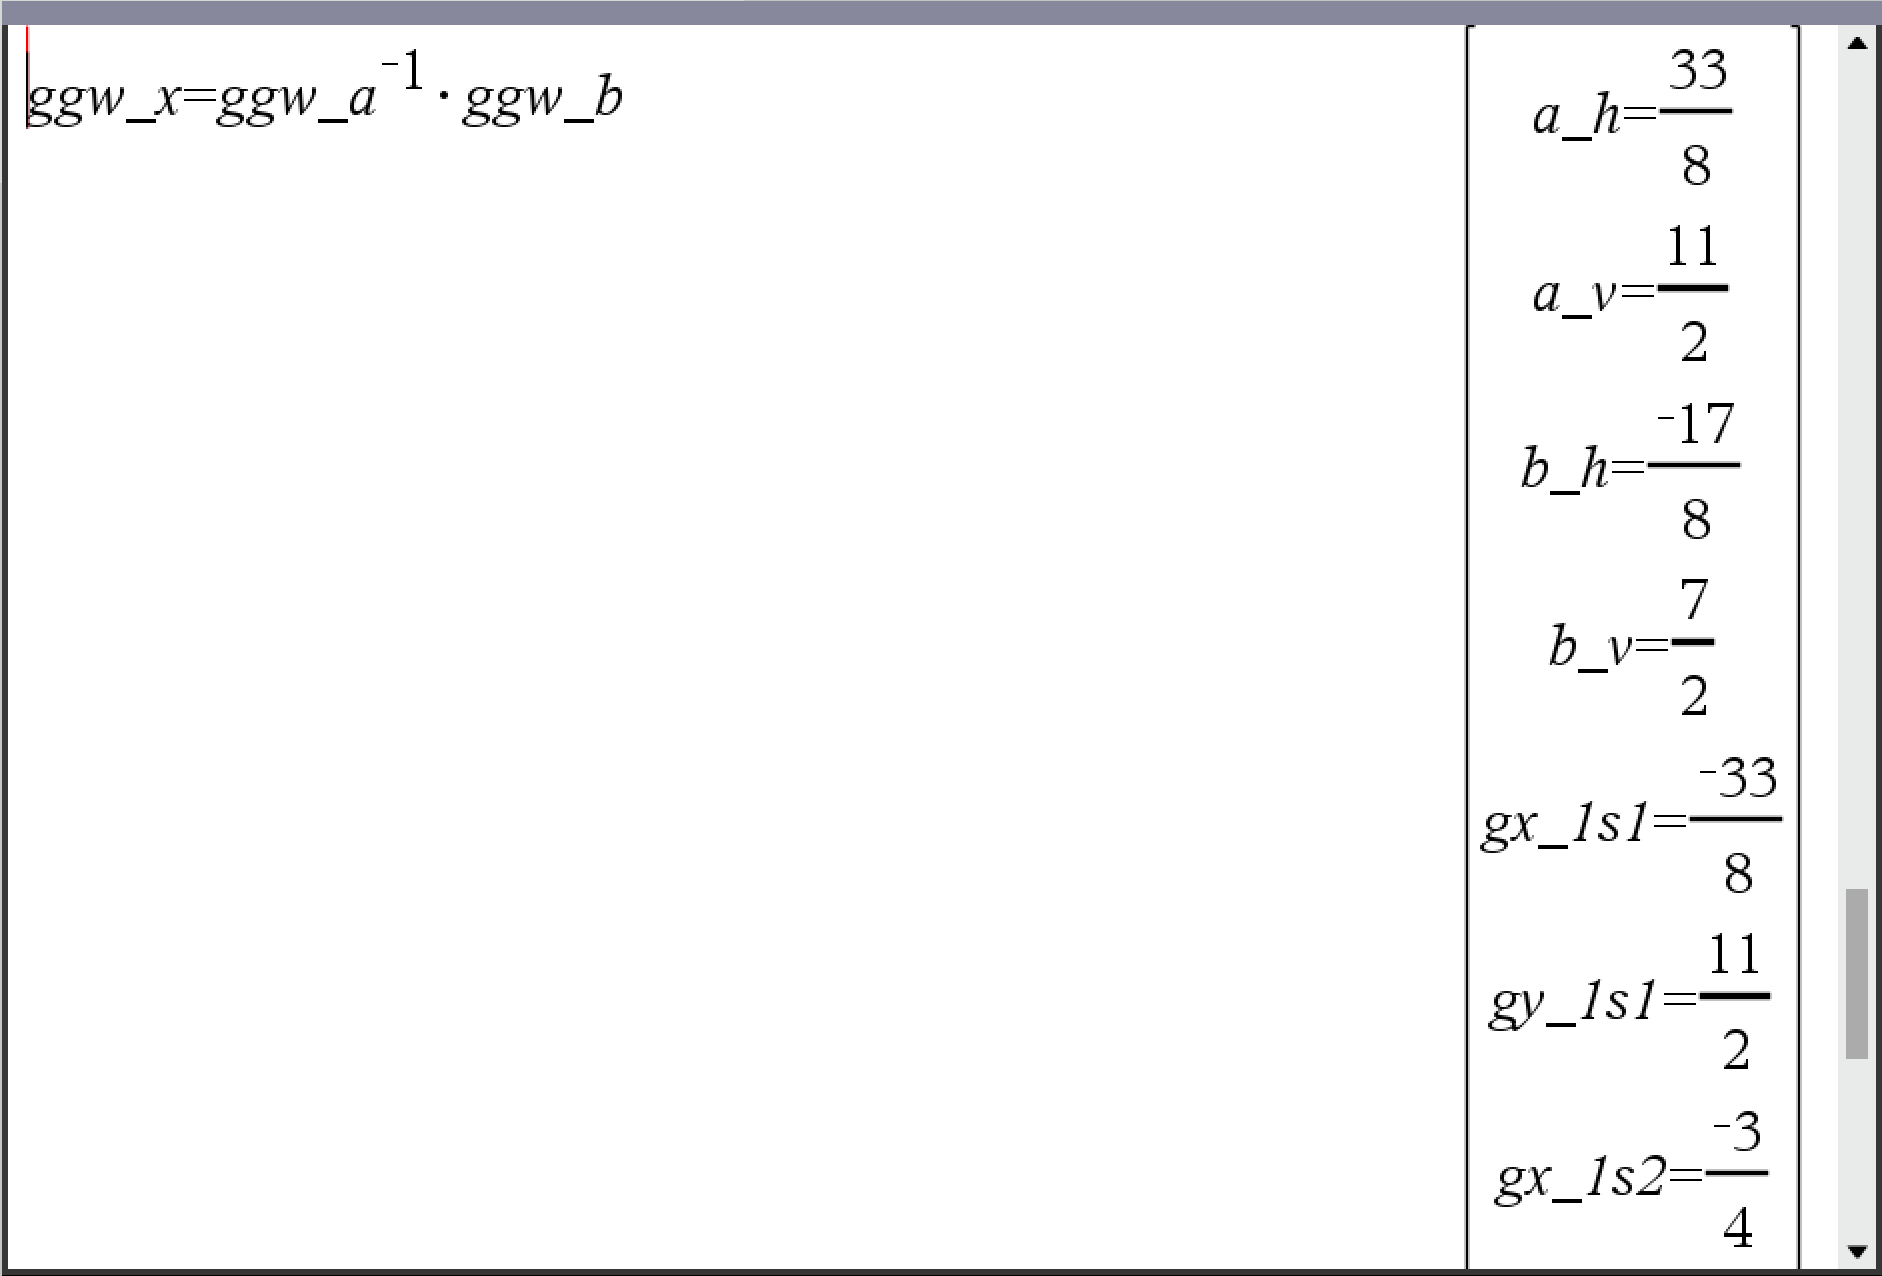
\includegraphics[width=\linewidth]{./fig/TM1/WiSe2122mr2_4.png}
        \caption{Lösung mit \code{ggw\_x}}
    \end{subfigure}
    \caption{WiSe~21/22, Nr.~2: exportiertes LGS}
    \label{fig:WiSe2122nr2_3}
\end{figure}

Die Explosionsansicht kann manchmal etwas unübersichtlich sein. Wenn ihr nah genug heranzoomt,
sollte aber trotzdem alles erkennbar sein. Die Ergebnisse müsst ihr natürlich nicht in dieser
Vektorform aufschreiben, nur ihr Inhalt zählt.

An dieser Stelle will ich anmerken, dass meist nur bei Systemen mit einem geschlossenen Ring wie
diesem nach allen Gelenk- und Auflagerkräften gefragt wird. Bei offenen Systemen ohne Ring wird oft
nur nach den Auflagerkräften gefragt. Das exportierte LGS liefert dann zwar auch die richtige Lösung, ist aber
meist mehr, als ihr braucht. Den Punkt, um den das Programm die Momentensumme eines Teilsystems
bildet, seht ihr, wenn ihr in der Explosionsansicht mit der Maus über das Teilsystem fahrt
(\emph{Hover}).

Die Zustandslinien, also die Verläufe der Schnittgrößen, zeichnet euch das Programm mit den Tasten
\taste{n}, \taste{q} und \taste{m}, die könnt ihr einfach abzeichnen. Falls ihr Randwerte schlecht
erkennt, fahrt mit der Maus über den jeweiligen Stab, dann zeigt das Programm nur noch diesen Stab
mit seinen Randwerten an.

\subsubsection{Qualitavtive Verläufe im symbolischen Modus (Nr.~4)}

Um meinen den oben genannten Punkt zum symbolischen Modus zu verdeutlichen will ich hier kurz auf Teilaufgabe b) eingehen.
Das System und der Querkraftverlauf sind in Abbildung~\ref{fig:TM1WiSe2122Nr4} dargestellt.

\begin{figure}[htbp]
    \centering
    \begin{subfigure}[t]{0.48\textwidth}
        \centering
        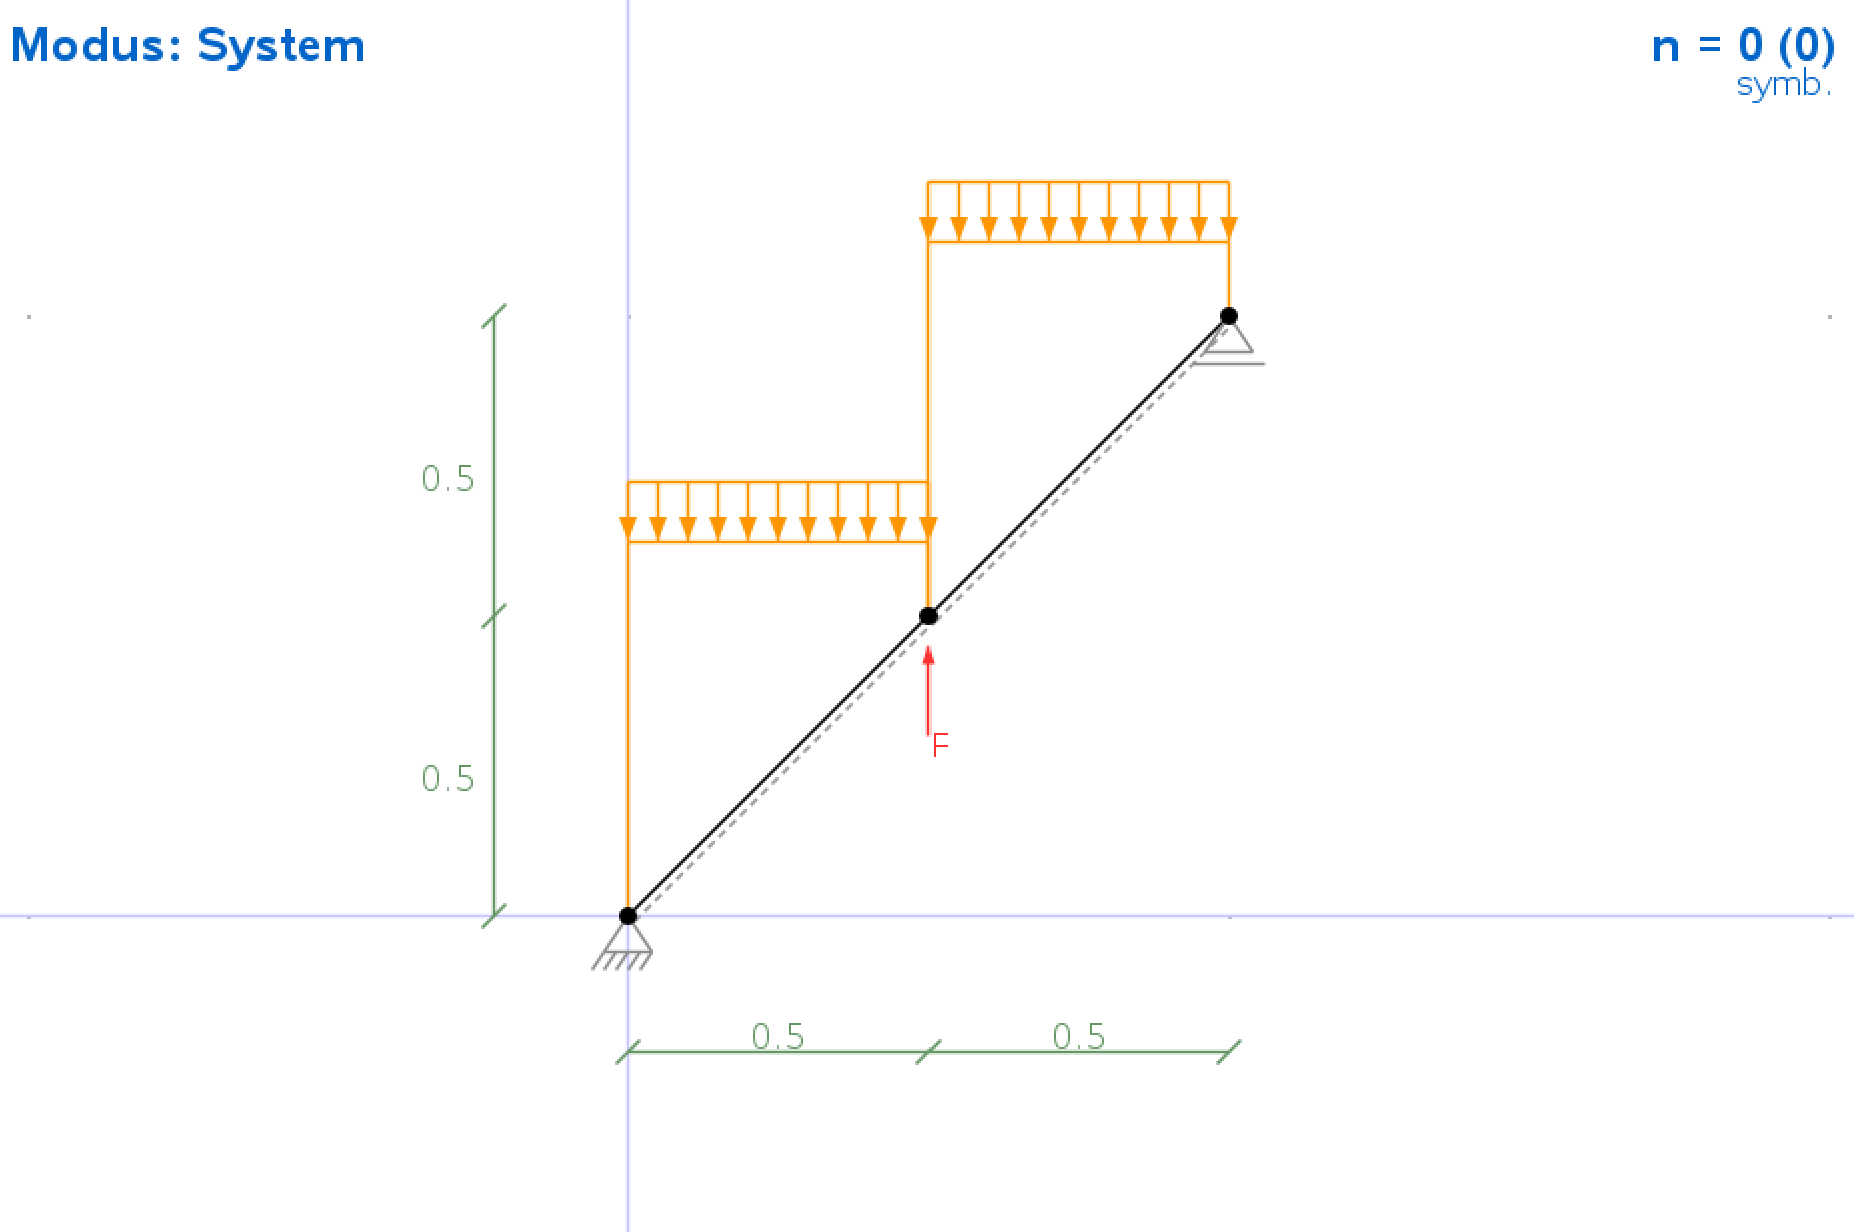
\includegraphics[width=\linewidth]{./fig/TM1/WiSe2122nr4_1.png}
        \caption{System}
    \end{subfigure}
    \hfill
    \begin{subfigure}[t]{0.48\textwidth}
        \centering
        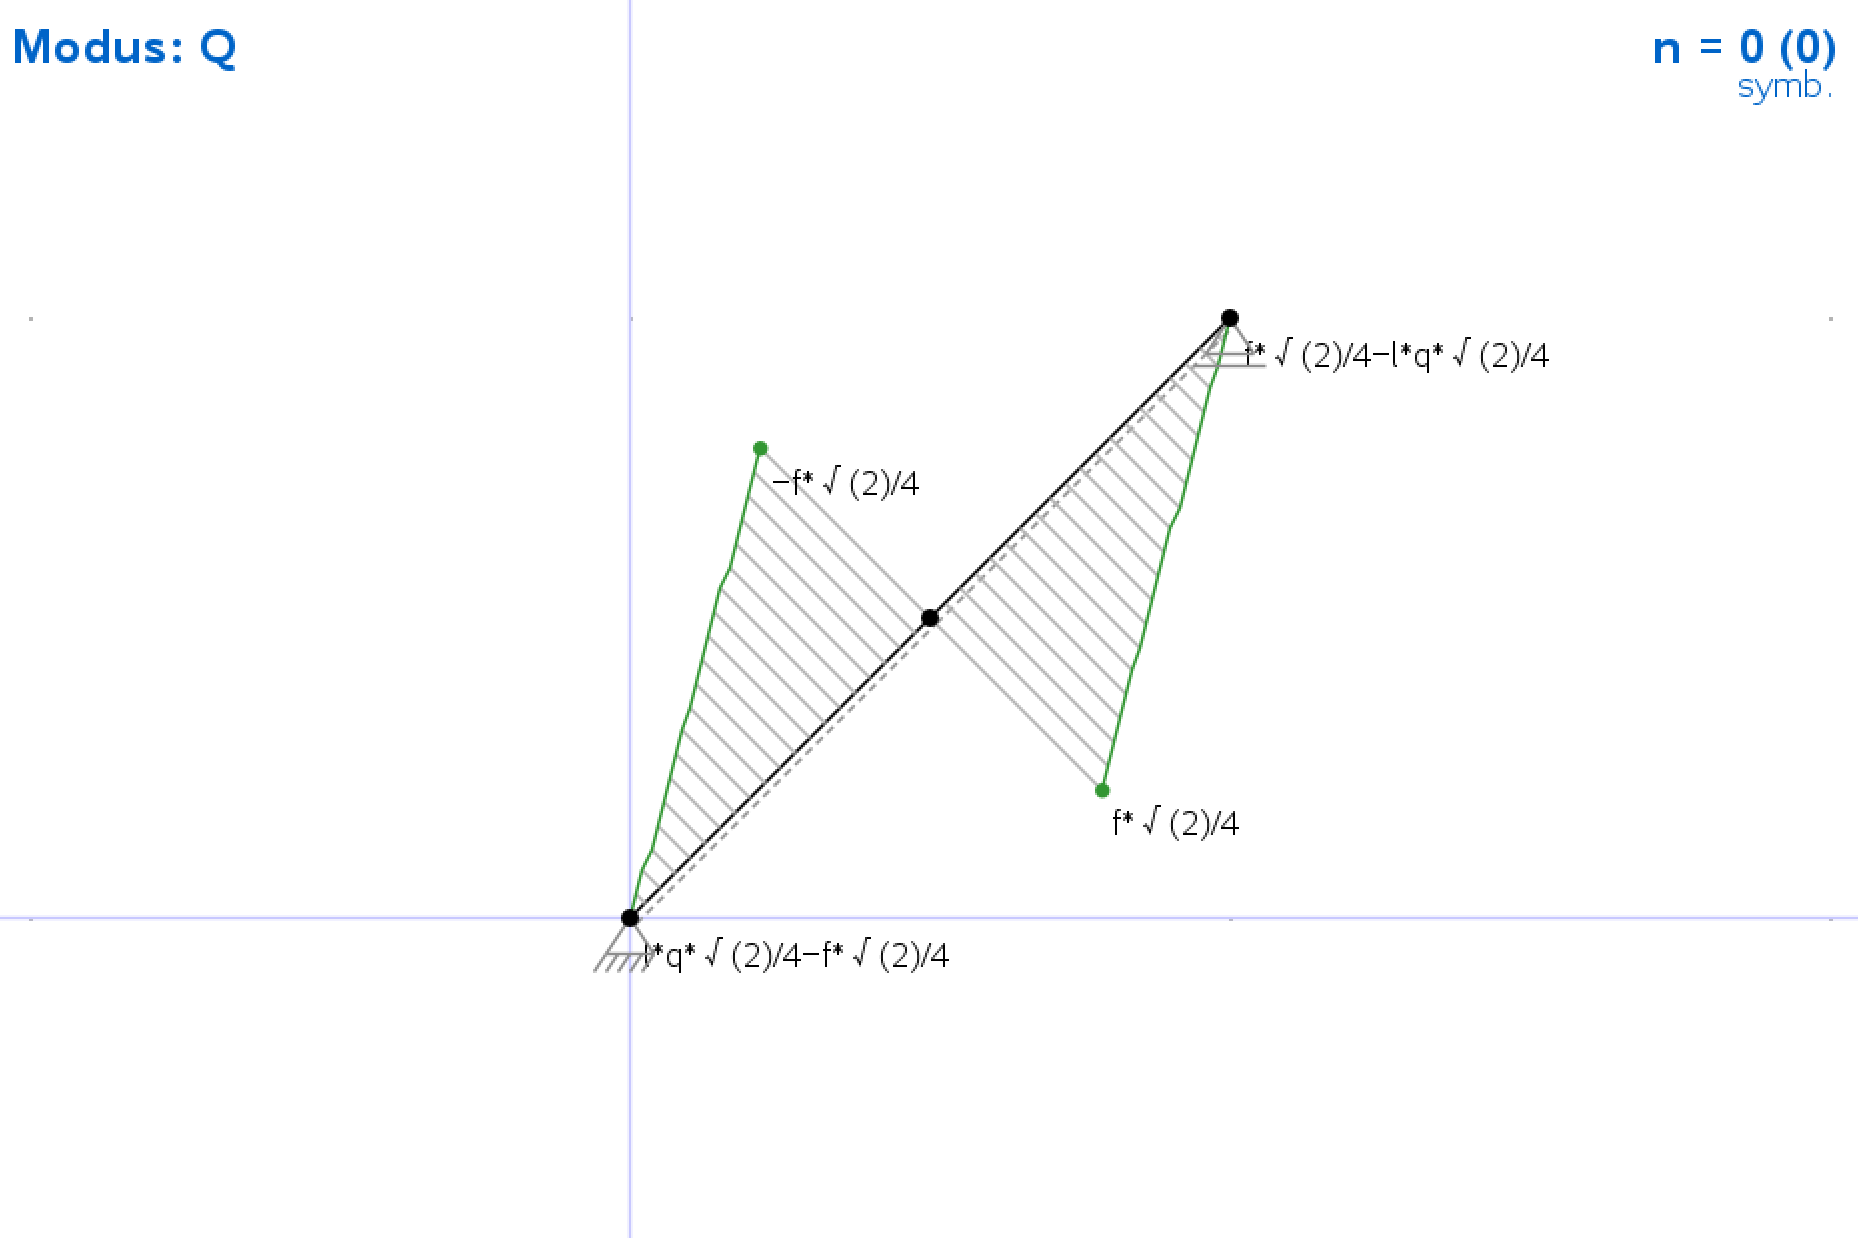
\includegraphics[width=\linewidth]{./fig/TM1/WiSe2122nr4_2.png}
        \caption{Querkraftverlauf}
    \end{subfigure}
    \caption{WiSe~21/22, Nr.~4}
    \label{fig:TM1WiSe2122Nr4}
\end{figure}

Im Querkraft verlauf sieht es so aus, als ob diese an den Auflagern null wird. Wenn man sich die Beschriftung der Randwerte 
anschaut wird jedoch klar, dass ist nur der Fall, wenn $q\cdot l=F$ bzw. $q\cdot a=F$ gilt. Das ist eben genau die Annhame des Programms,
um überhaupt irgendeinen Verlauf zeichnen zu können.
Die Aufgabe gibt aber unten vor: $F>q\cdot a$. Damit wird die Qerkraft am linekn Ende negativ und am rechten Ende positiv.
Die Verläufe von symbolische Berechnungen solltet ihr also \textbf{nie} einfach blind abzeichnen.

\subsection{PvV (Nr.~3)}

Zum PvV gibt es eigentlich nicht viel zu sagen. System zeichnen, \taste{v} drücken, Bindung wählen, abzeichnen,
dann exportieren und aufschreiben. 


\begin{figure}[htbp]
    \centering
    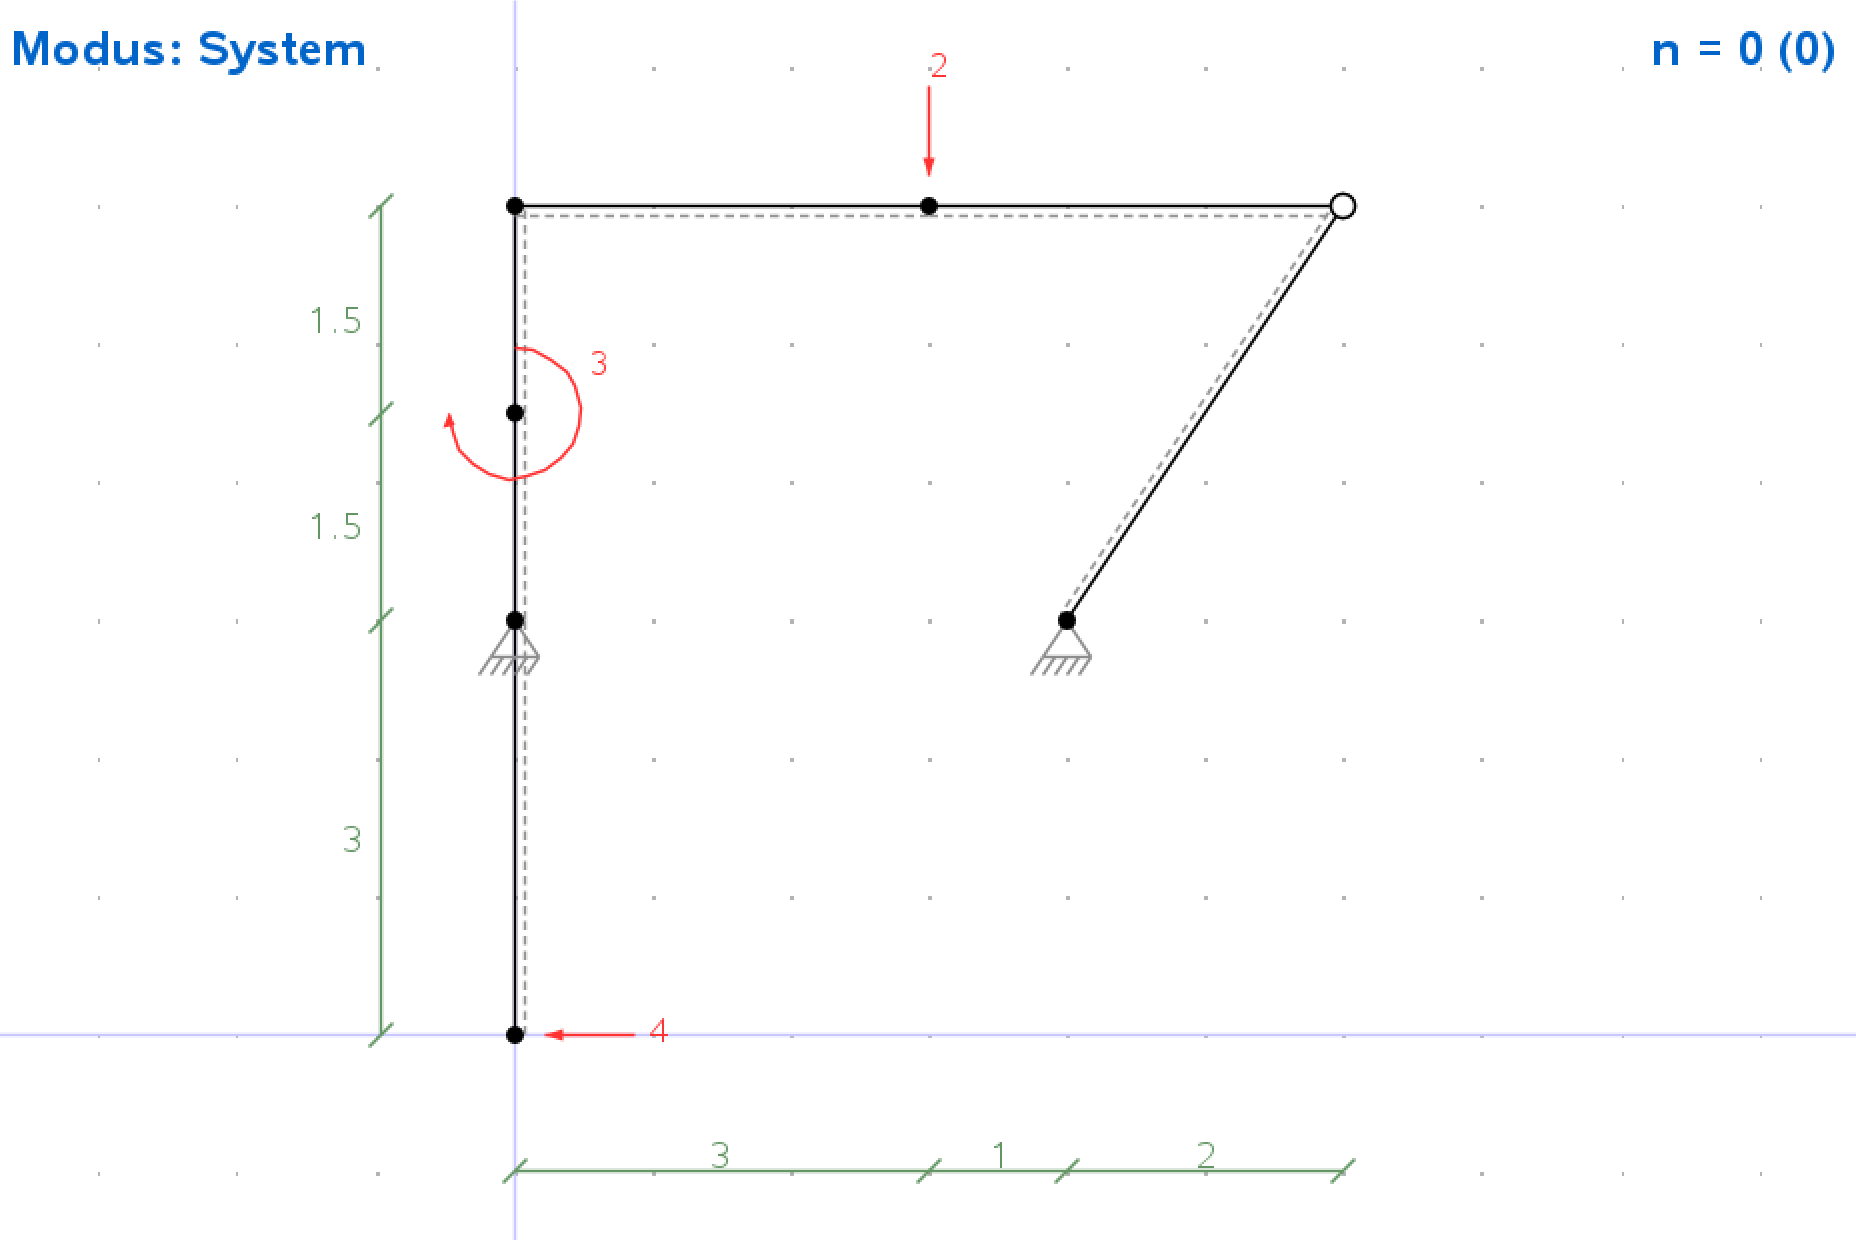
\includegraphics[width=0.5\linewidth]{./fig/TM1/WiSe2122nr3_1.png}
    \caption{TM1 WiSe~21/22, Nr.~3 im Programm}
    \label{fig:TM1WiSe2122Nr3_1}
\end{figure}

\begin{figure}[htbp]
    \centering
    \begin{subfigure}[t]{0.48\textwidth}
        \centering
        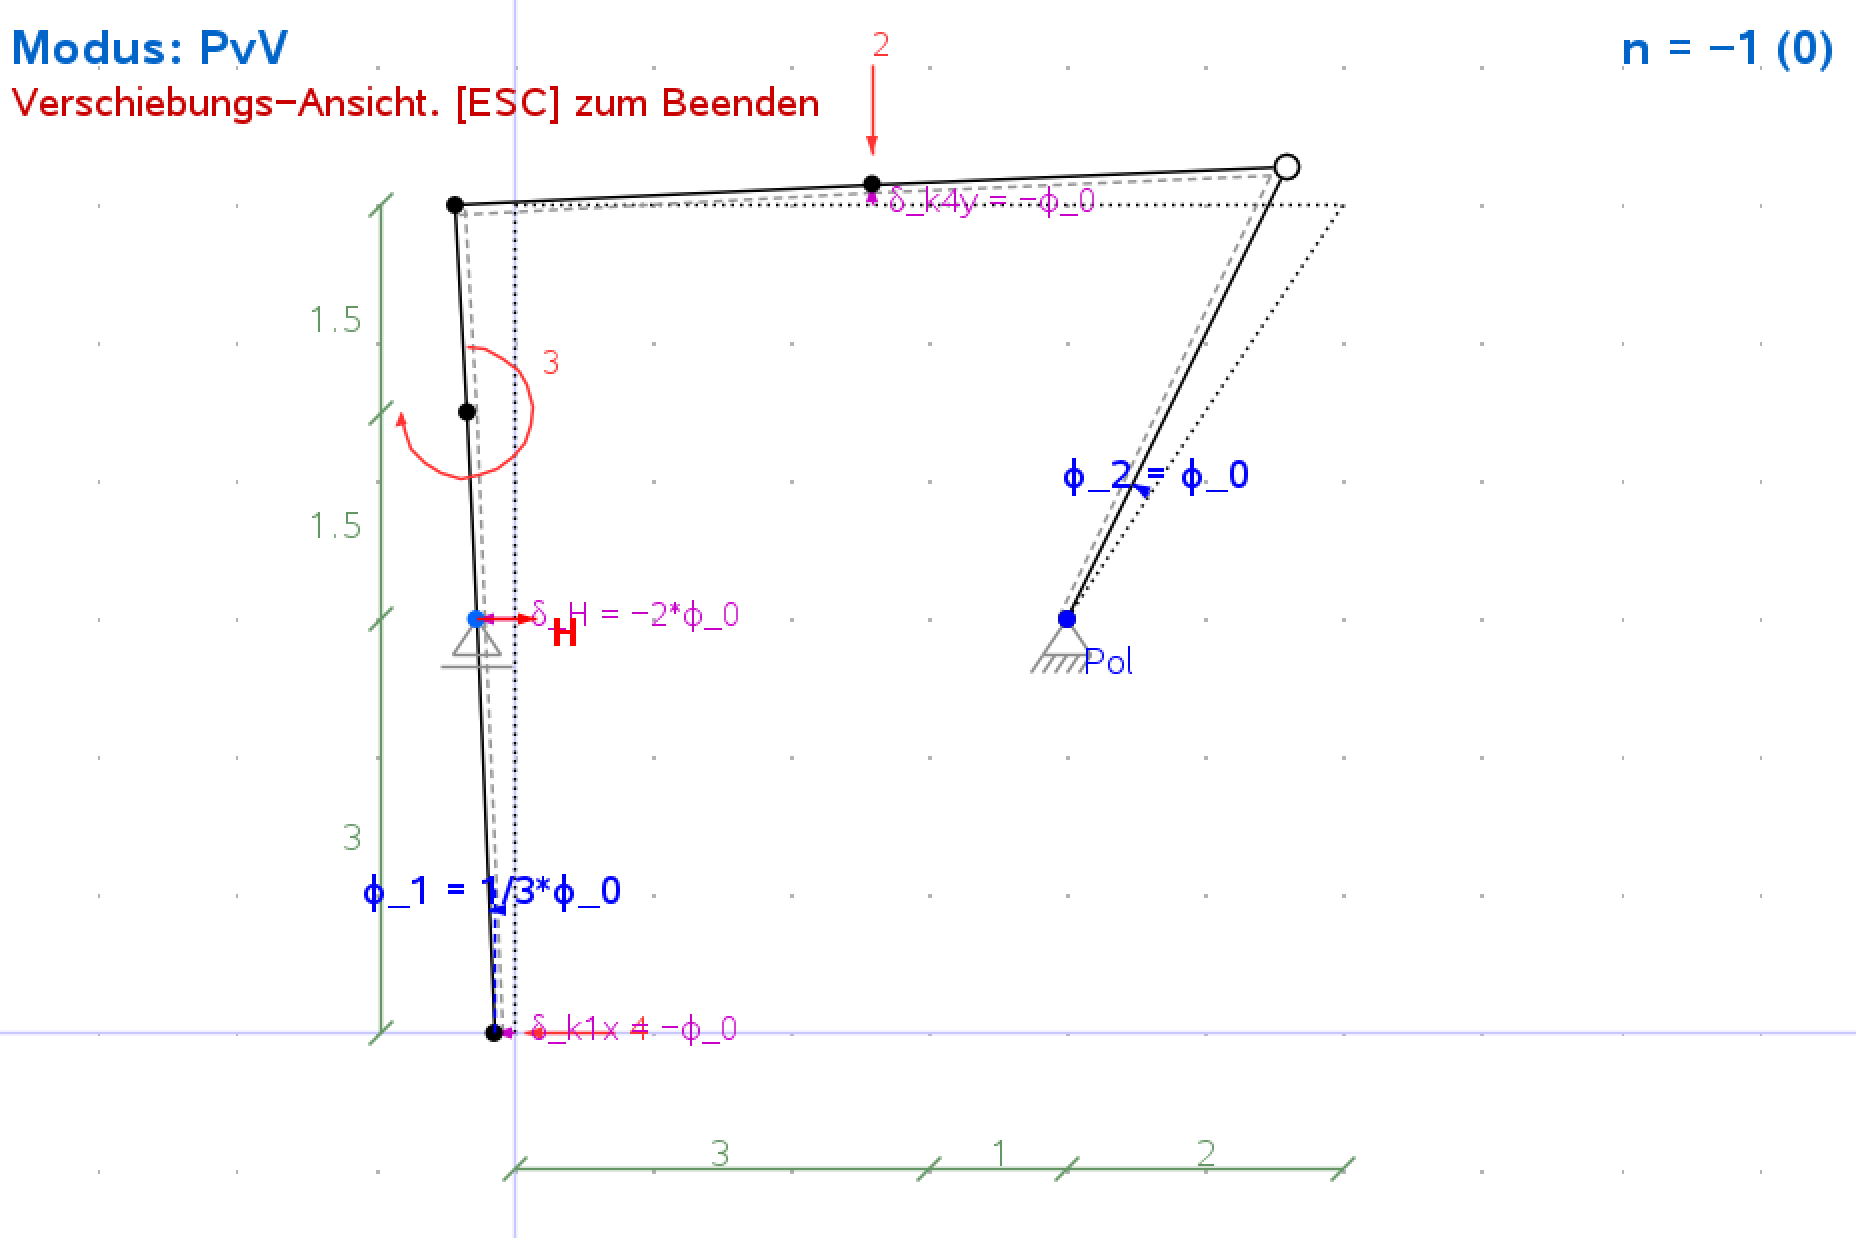
\includegraphics[width=\linewidth]{./fig/TM1/WiSe2122nr3_2.png}
        \caption{Verschiebungsfigur für $A_H$}
    \end{subfigure}
    \hfill
    \begin{subfigure}[t]{0.48\textwidth}
        \centering
        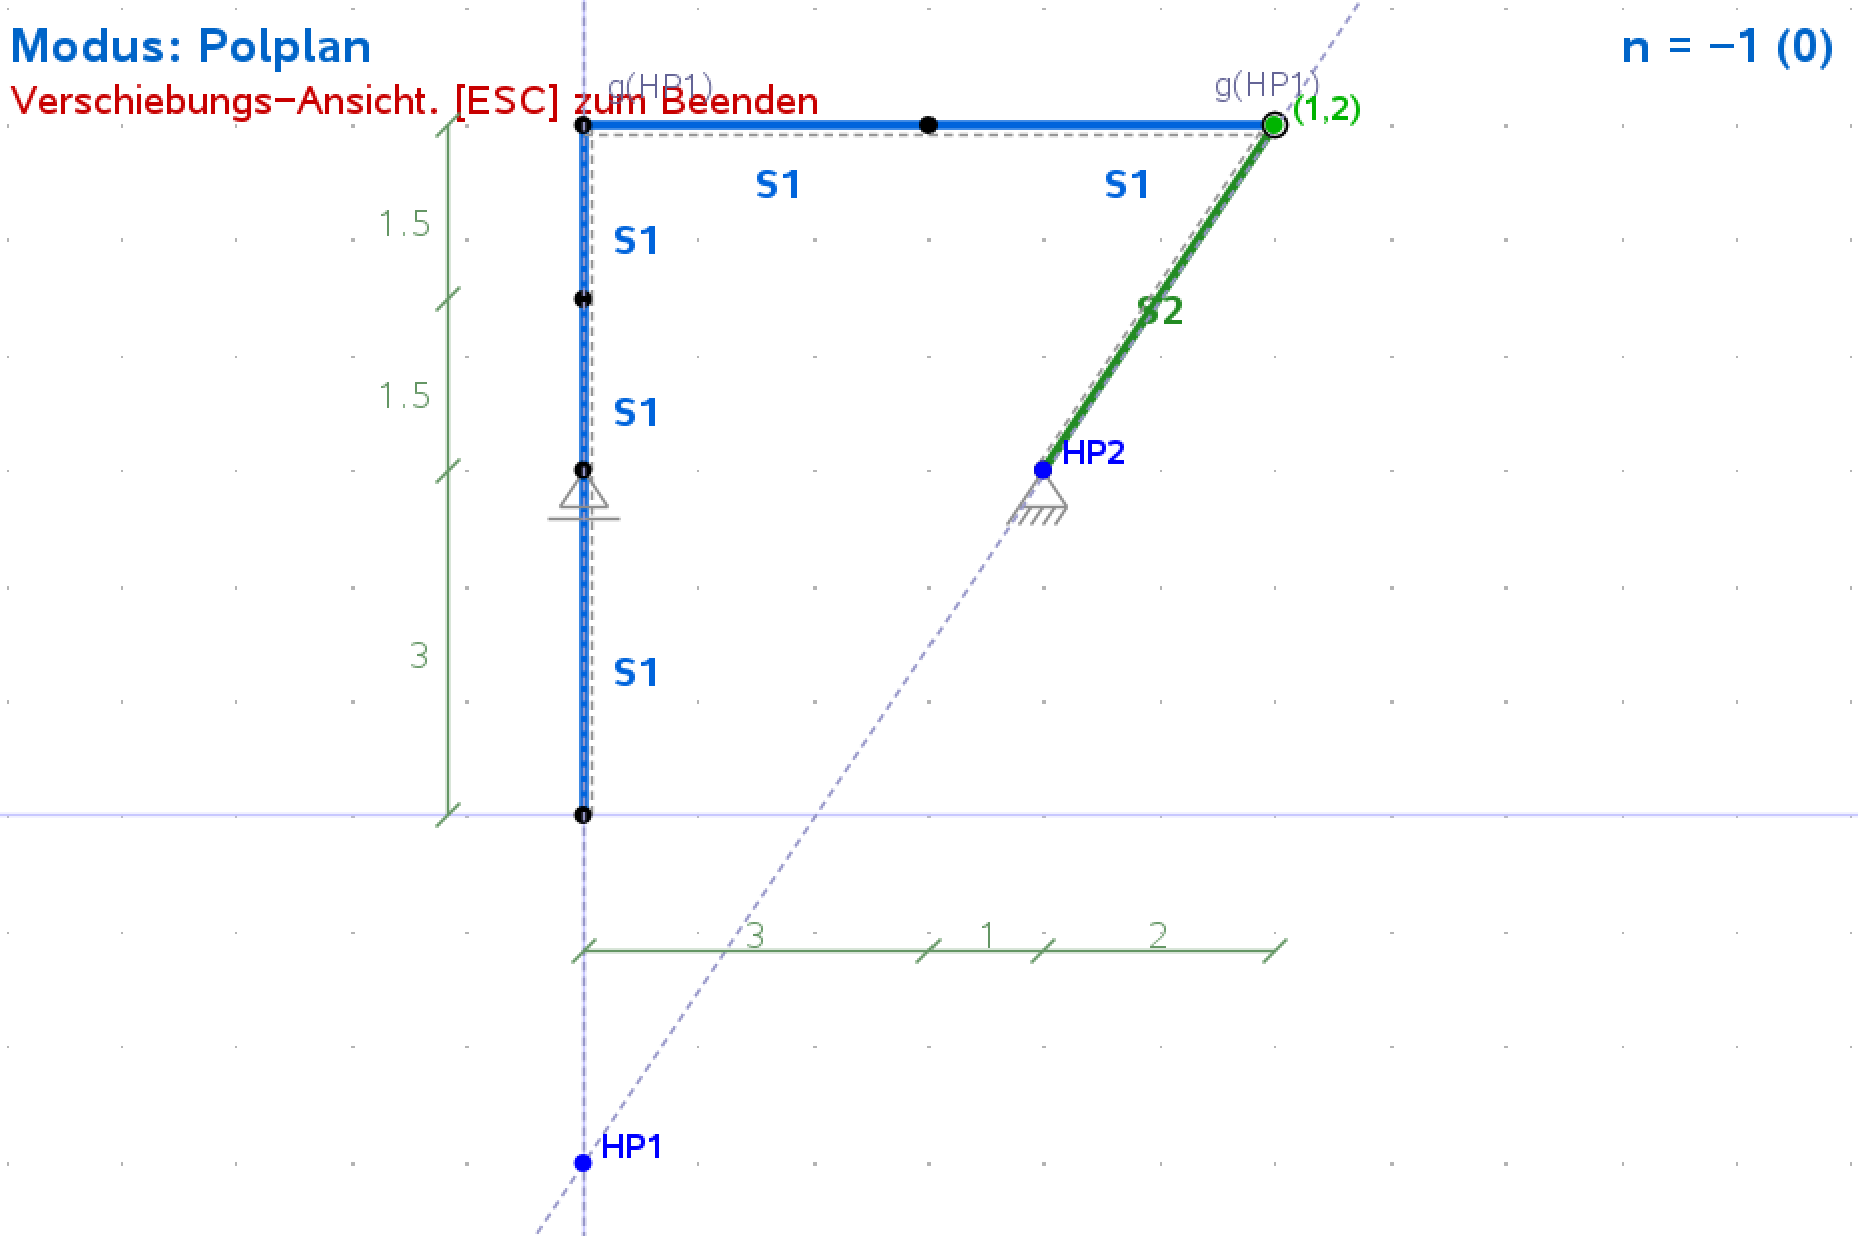
\includegraphics[width=\linewidth]{./fig/TM1/WiSe2122nr3_3.png}
        \caption{Polplan für $A_H$}
    \end{subfigure}
    \caption{WiSe~21/22, Nr.~3: $A_H$}
    \label{fig:TM1WiSe2122Nr3_2}
\end{figure}

\begin{figure}[htbp]
    \centering
    \begin{subfigure}[t]{0.48\textwidth}
        \centering
        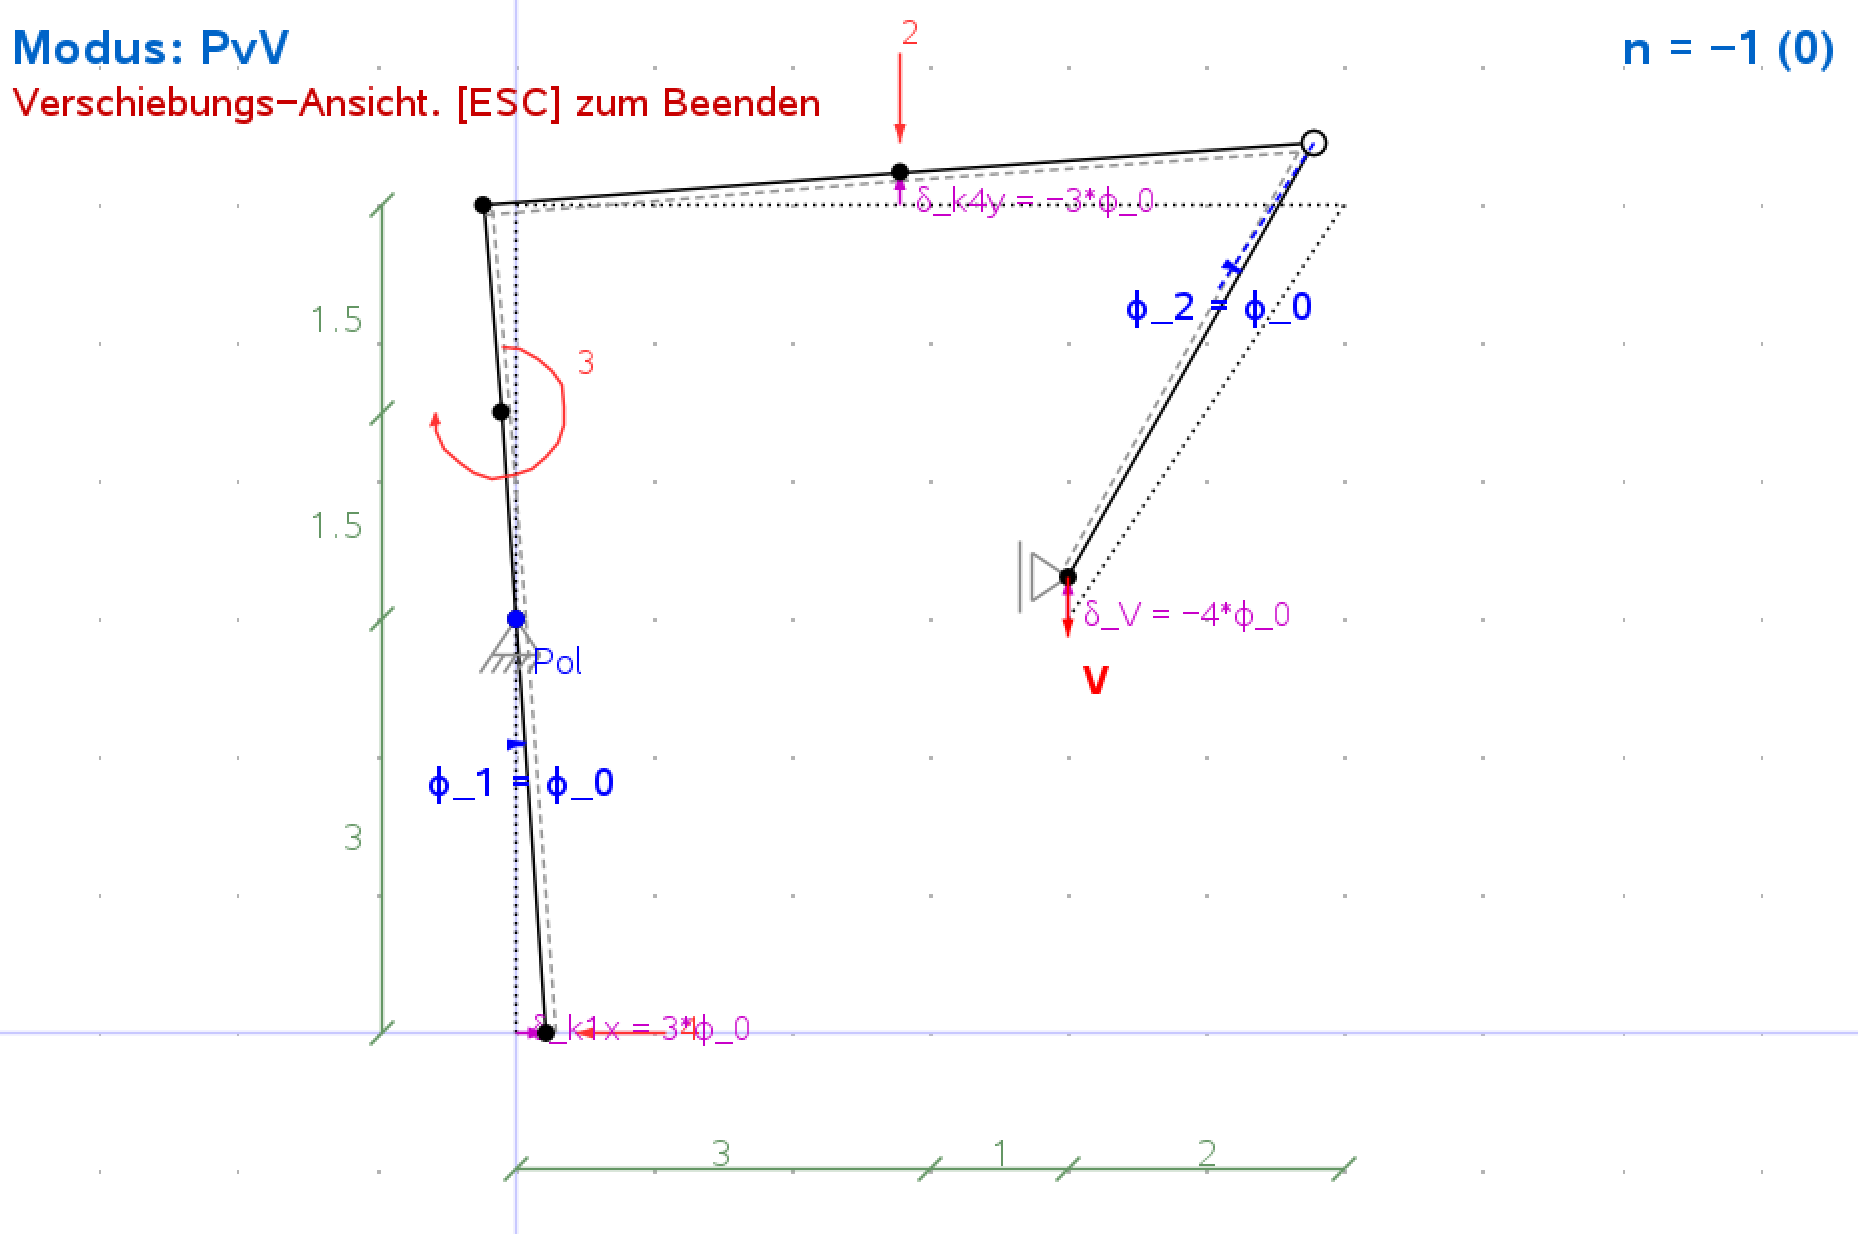
\includegraphics[width=\linewidth]{./fig/TM1/WiSe2122nr3_4.png}
        \caption{Verschiebungsfigur für $B_V$}
    \end{subfigure}
    \hfill
    \begin{subfigure}[t]{0.48\textwidth}
        \centering
        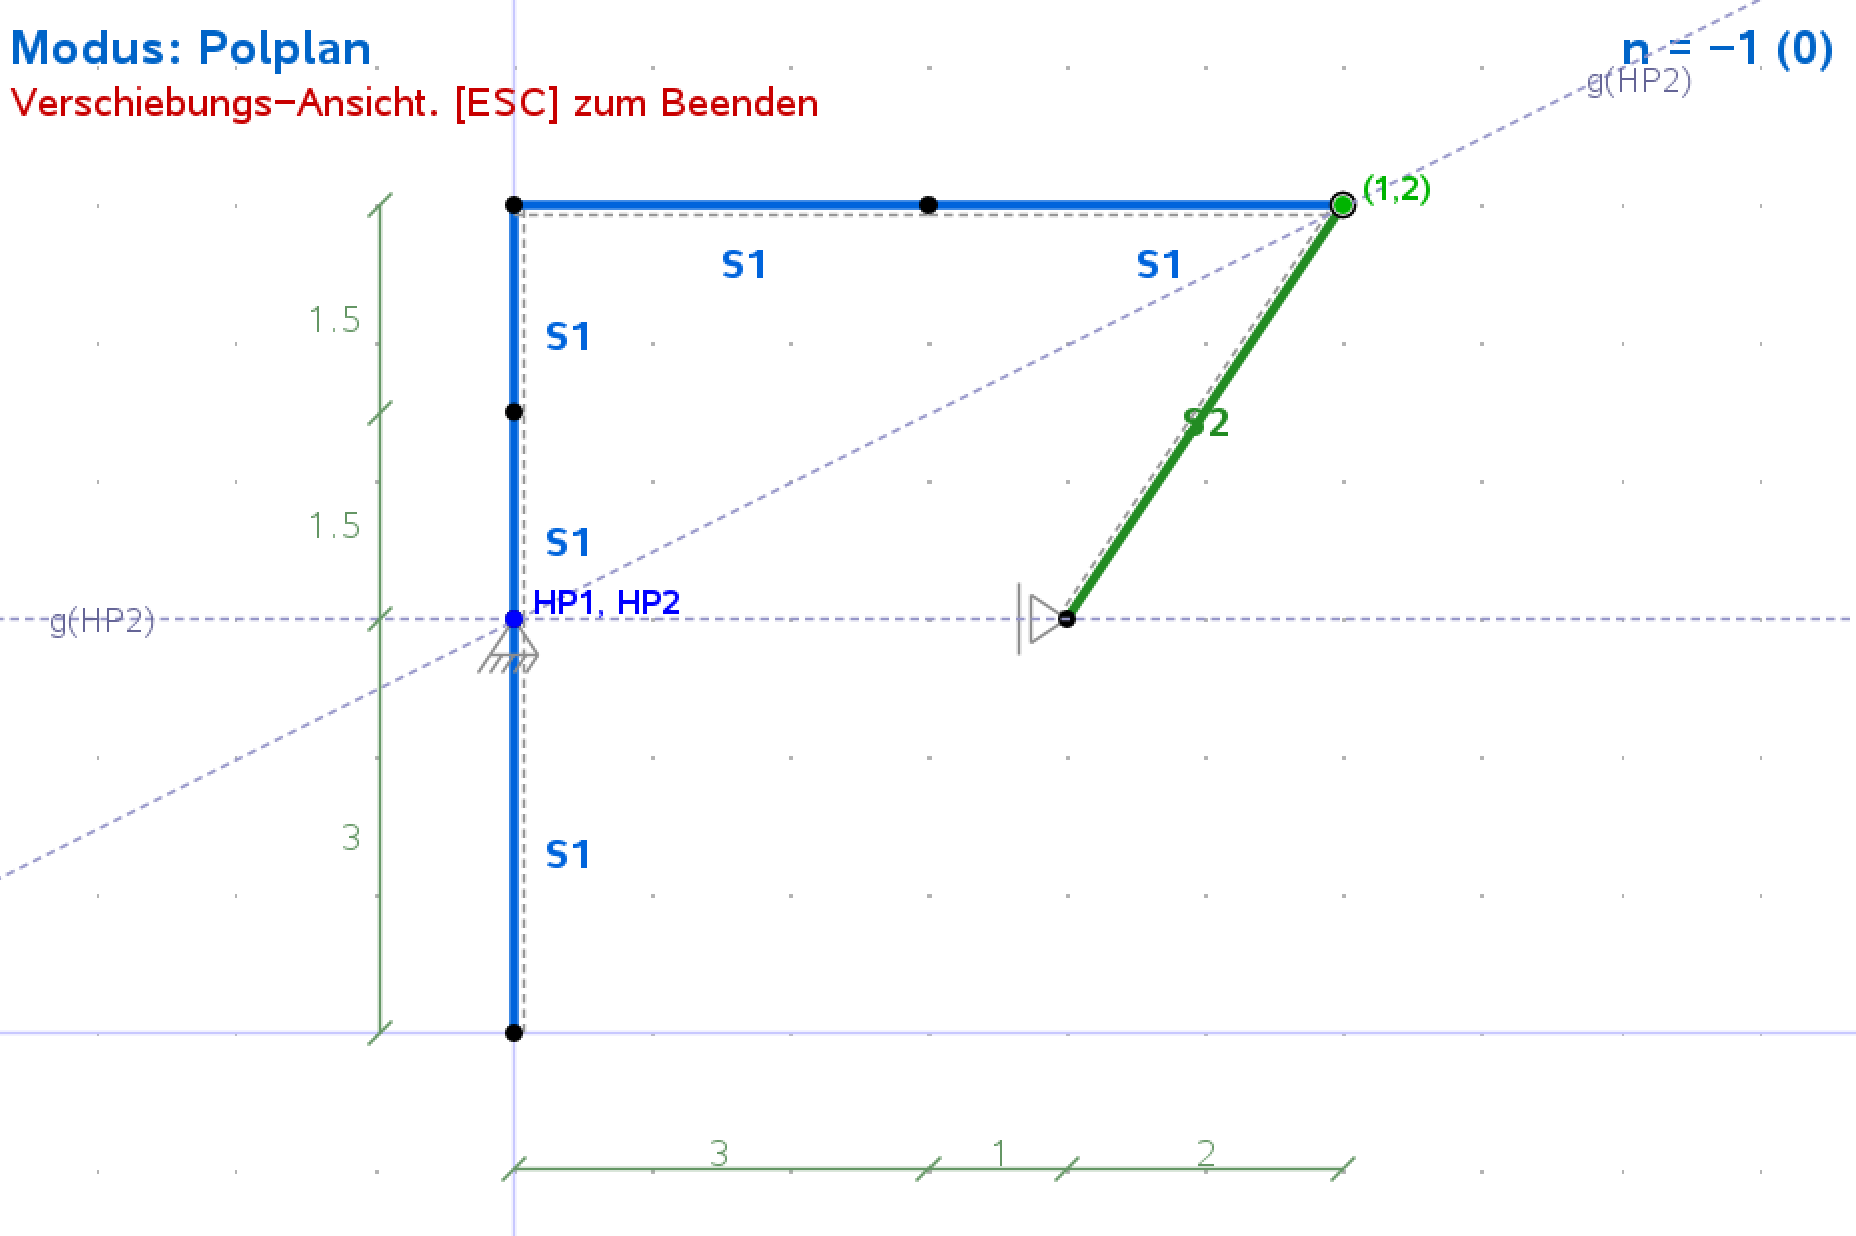
\includegraphics[width=\linewidth]{./fig/TM1/WiSe2122nr3_5.png}
        \caption{Polplan für $B_V$}
    \end{subfigure}
    \caption{WiSe~21/22, Nr.~3: $B_V$}
    \label{fig:TM1WiSe2122Nr3_3}
\end{figure}

Die Zeilen der Matrizen \code{pvv\_kin} und \code{pvv\_pol} (Abb.~\ref{fig:TM1WiSe2122Nr3_4})
sind als Gleichungskette zu lesen. Hier gilt also z.B. $\delta_{k1x}= -3\cdot\varphi_1=-\varphi_0$, oder 
$\delta x_{p12}= -9\cdot\varphi_1=-3\varphi_2$. Mit diesen Gleichungen lässt sich aus \code{w\_eq1} \code{w\_eq2} bauen.
Diese gleichung lässt sich dann entweder von hand oder mit dem Taschenrechner nach der gesuchten Größe auflösen.

\begin{figure}[htbp]
    \centering
    \begin{subfigure}[t]{0.48\textwidth}
        \centering
        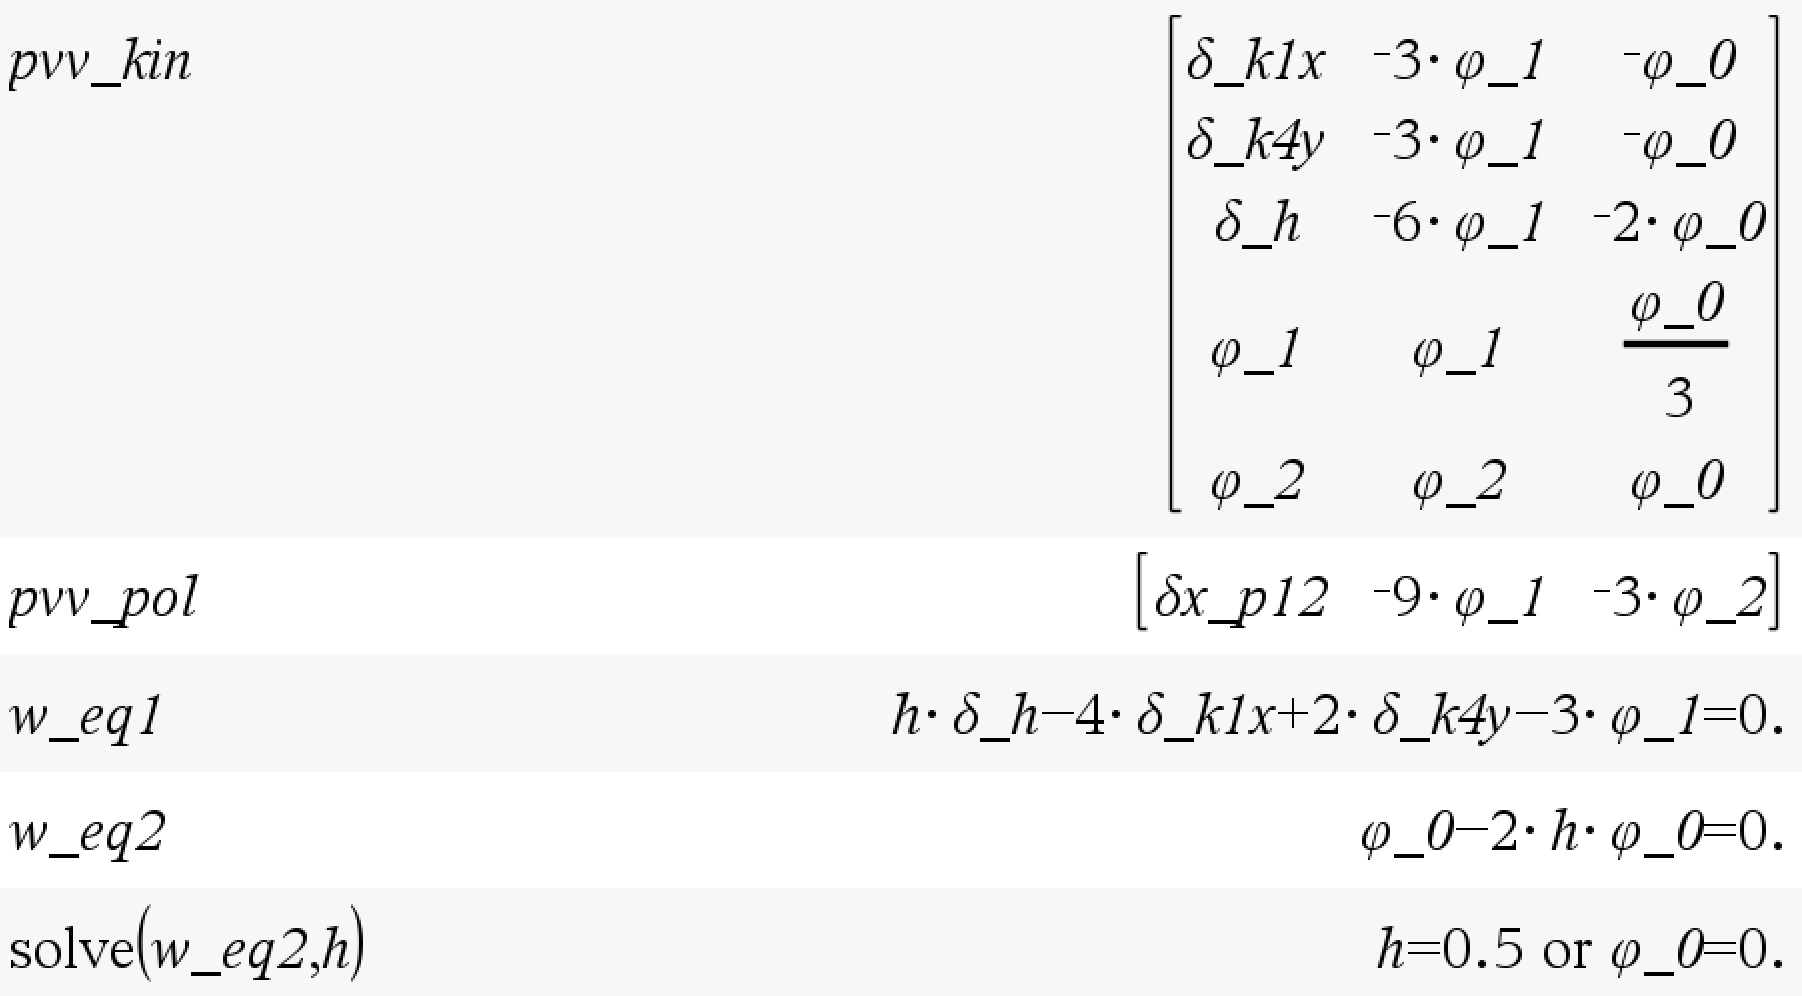
\includegraphics[width=\linewidth]{./fig/TM1/WiSe2122nr3_6.png}
        \caption{Rechnung für $A_H$}
    \end{subfigure}
    \hfill
    \begin{subfigure}[t]{0.48\textwidth}
        \centering
        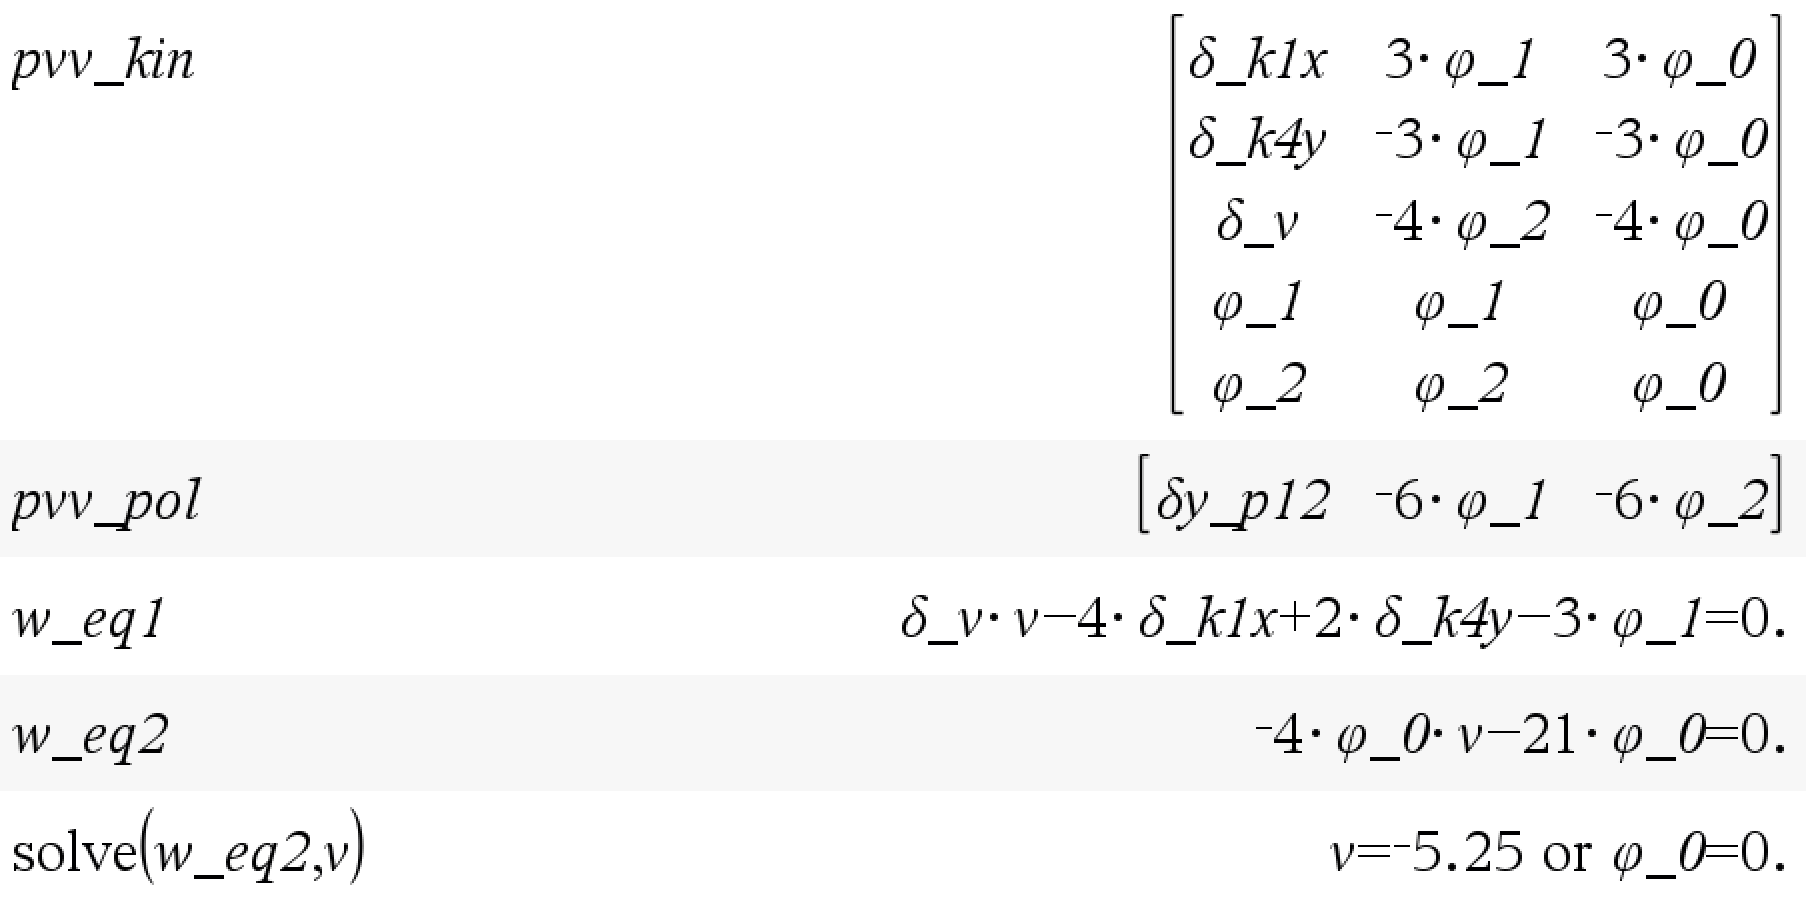
\includegraphics[width=\linewidth]{./fig/TM1/WiSe2122nr3_7.png}
        \caption{Rechnung für $B_V$}
    \end{subfigure}
    \caption{WiSe~21/22, Nr.~3: Ergebnis}
    \label{fig:TM1WiSe2122Nr3_4}
\end{figure}

\subsection{Schnittkräfte Bögen (Nr.~5)}

Mit dem Programm lassen sich die Funktionen für Schnittkraftverläufe von normalen Stäben als auch von Bögen 
ausgeben. Bei bögen ist die Laufvraibale nur nicht mehr die Länge entlang des Stabes sondern der Winkel.
also für diese Aufgabe zweilmal $\varphi \in [0,\frac{\pi}{4}]$ bzw. $\varphi \in [0,90\text{°}]$. Hier ist die Winkel-Einstellung
des Taschenrechenrs wichtig.\\
Hier gilt aber auch wieder, dass das Programm das nicht wirklich so ausrechnet wie man das von Hand machen würde, sondern
es sucht eine schöne Darstellung der Anfangswerte und kombiniert diese dann zur Funktion.

\begin{figure}[htbp]
    \centering
    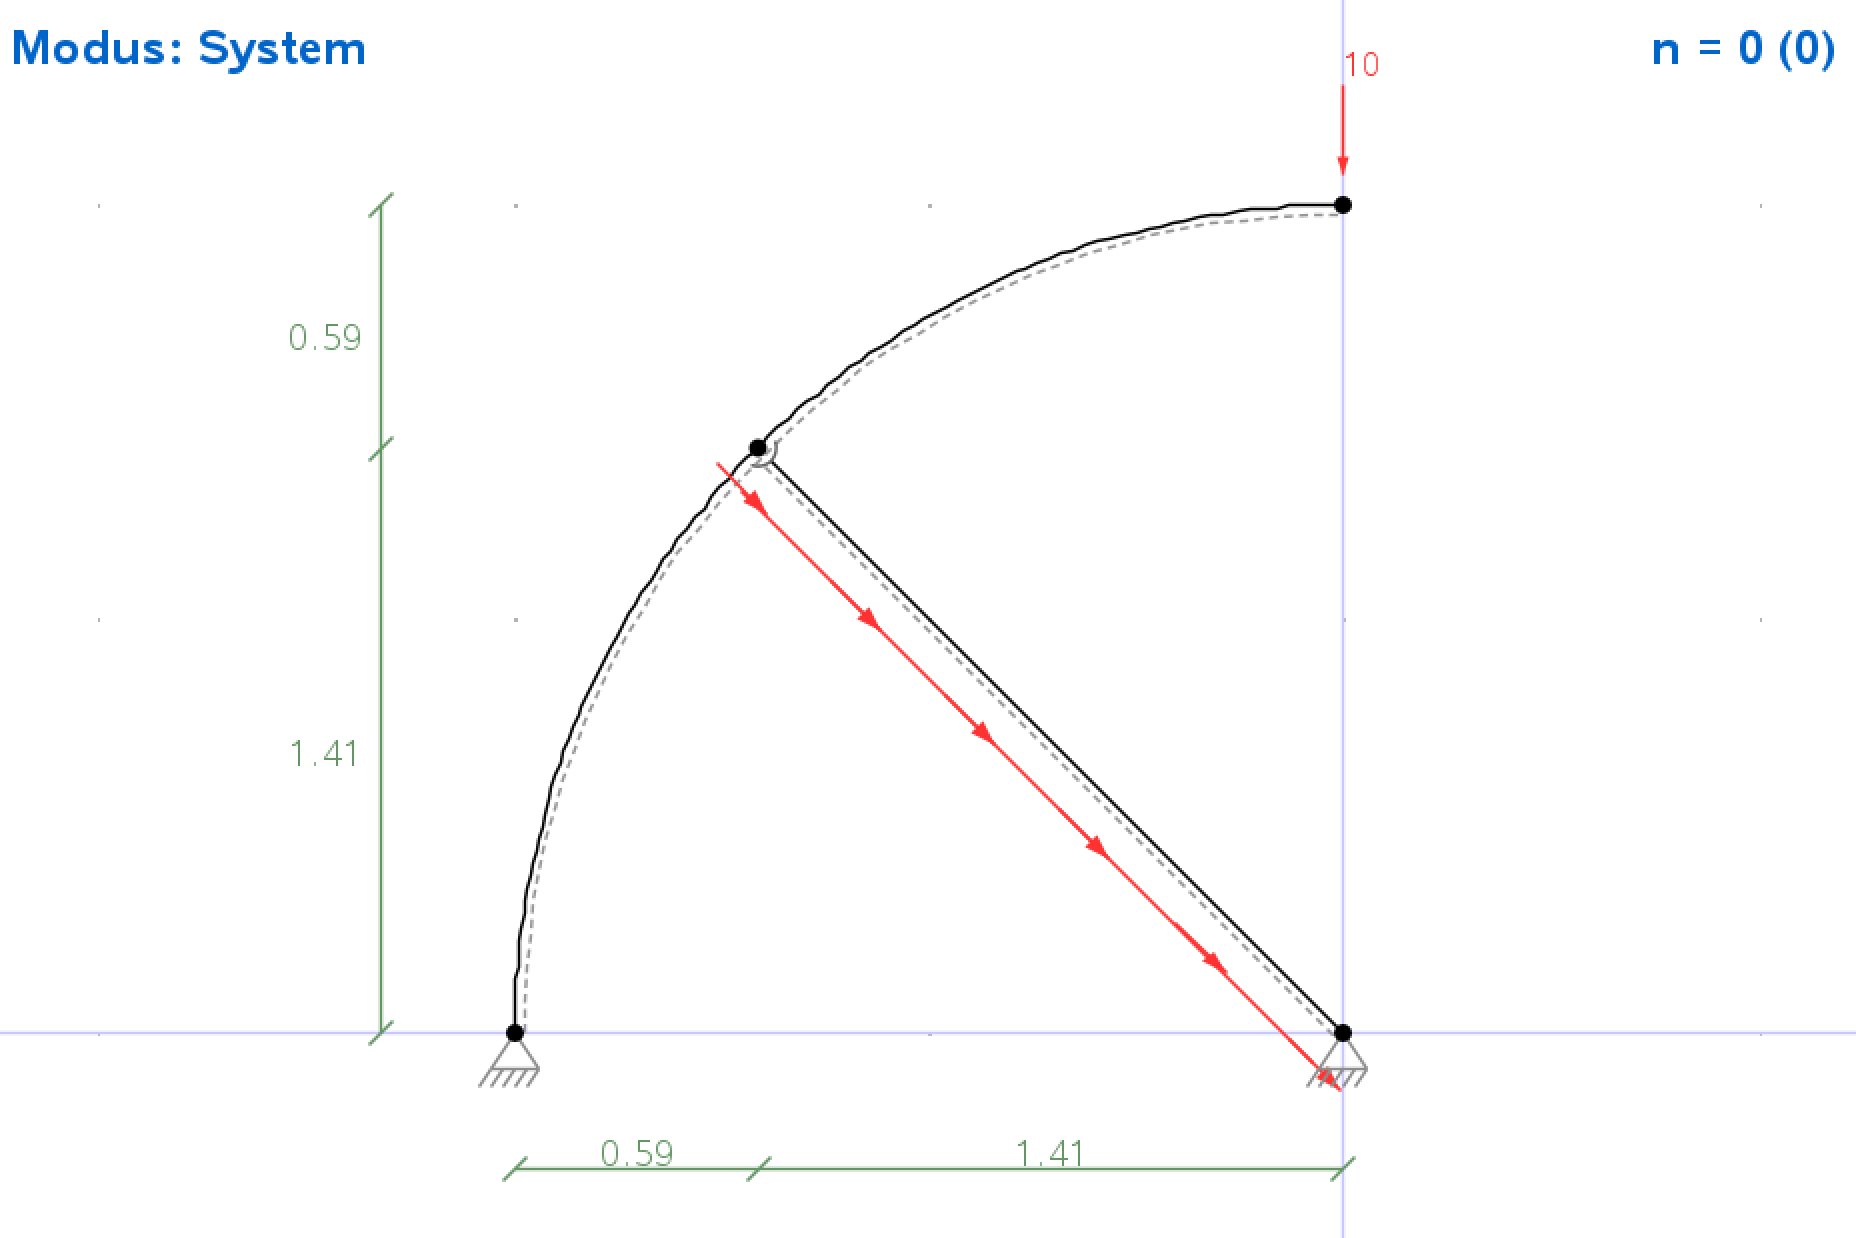
\includegraphics[width=0.5\linewidth]{./fig/TM1/WiSe2122nr5_1.png}
    \caption{TM1 WiSe~21/22, Nr.~5 im Programm}
    \label{fig:TM1WiSe2122Nr5_1}
\end{figure}


\subsection{Fachwerk (Nr.6)}

Vom Prinzip werden Fachwerke genau gleich eingegeben wie normale Systeme, nur das hier die orientierung der gestrichelten Faser
keine Rolle spielt. Es ist jedoch sinnvoll den Fachwerk Modus anzumachen, dann wird die statische Bestimmtheit beim hovern über $n=$ 
auch die Formel für Fachwerke verwendet und alle Knoten werden zu vollgelenken gemacht, auch wenn der Modus erst nach dem 
zeichnen des Systems angemacht wird.  


\begin{figure}[htbp]
    \centering
    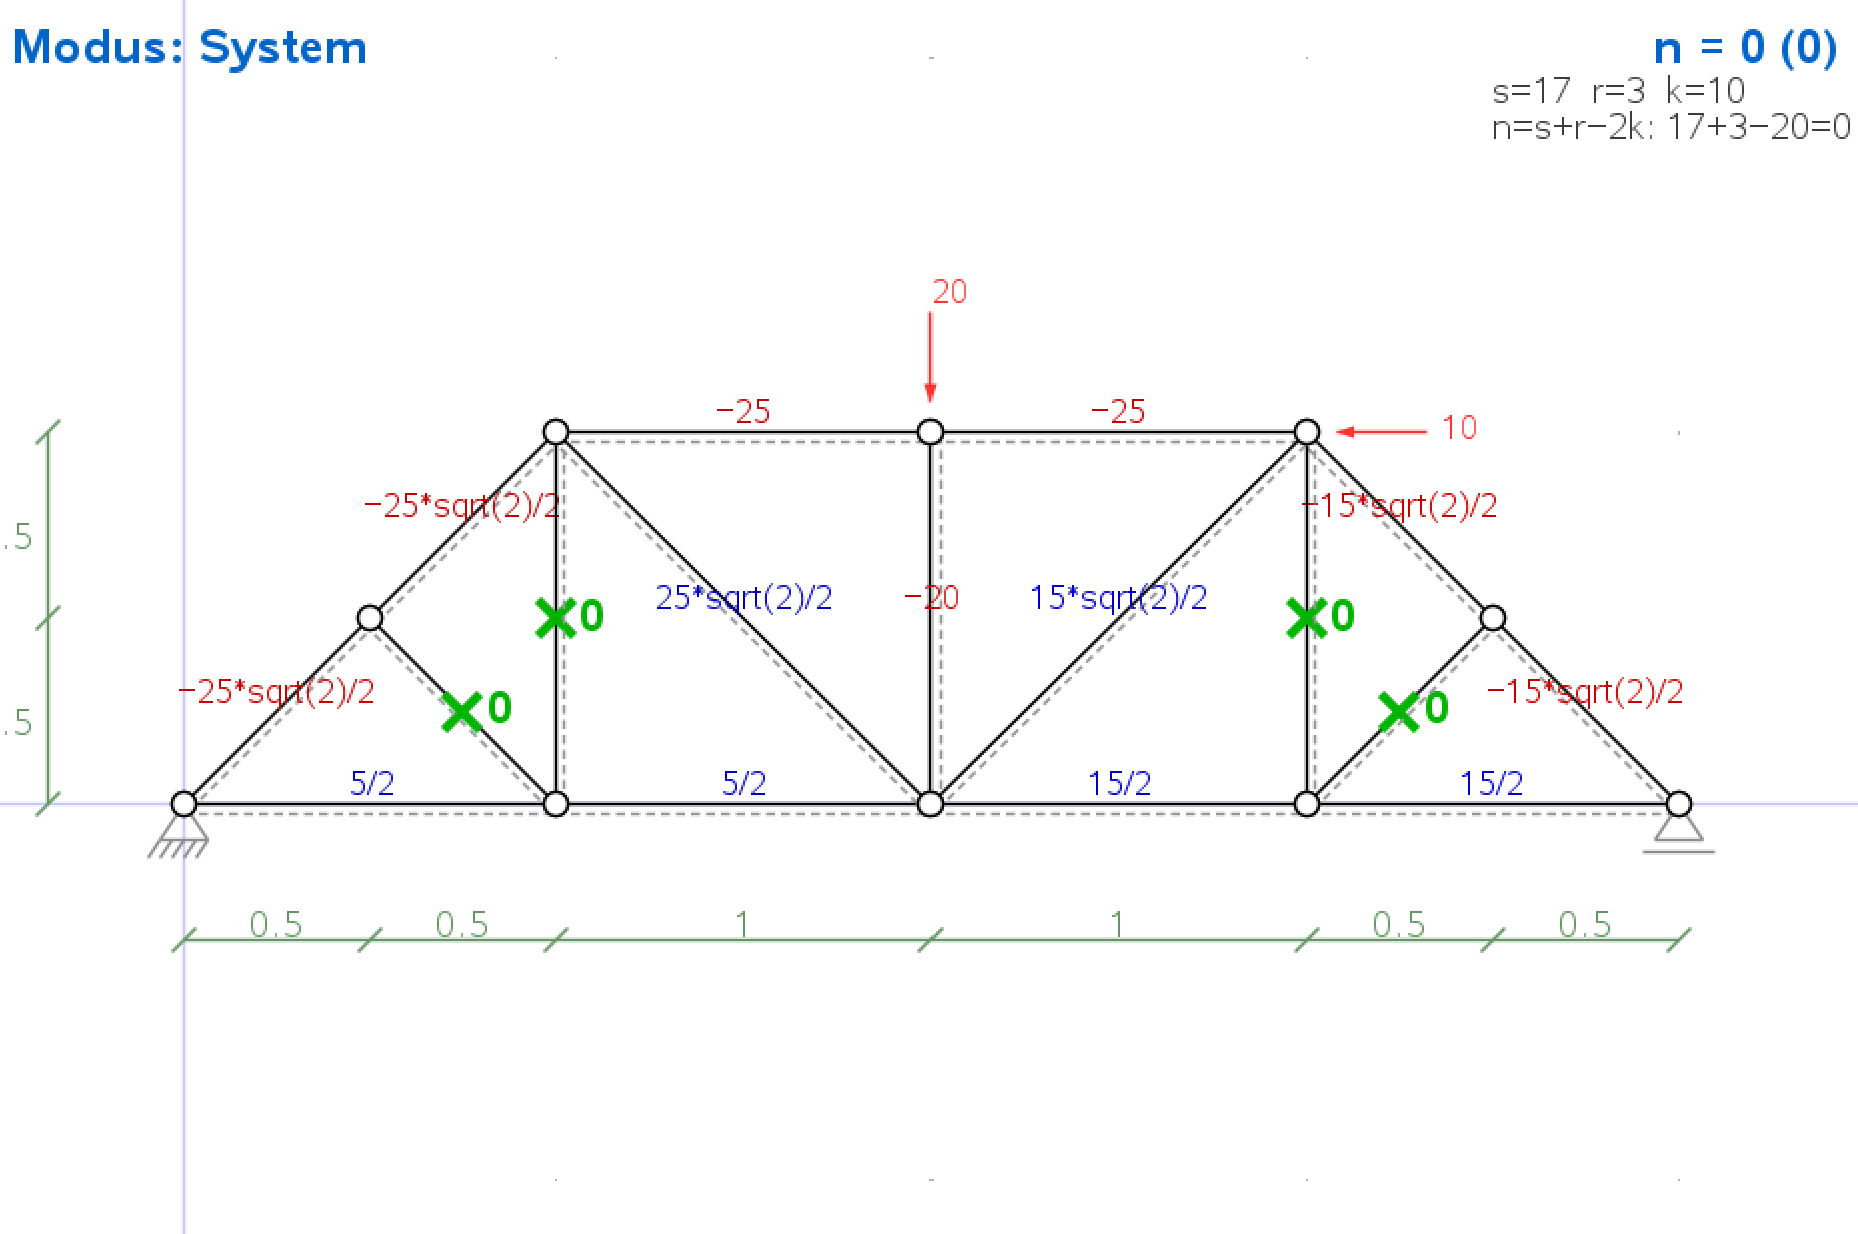
\includegraphics[width=0.5\linewidth]{./fig/TM1/WiSe2122nr6_1.png}
    \caption{TM1 WiSe~21/22, Nr.~6 im Programm}
    \label{fig:TM1WiSe2122Nr6_1}
\end{figure}

Die Stabe in Abb.~\ref{fig:TM1WiSe2122Nr6_1} die ein grünes Kreuz haben sind die ohne Rechnung erkennbaren Nullstäbe
Falls nach der Berechnung stäbkkräfte mit einer grünen Null beschriftet werdsen, aber dort kein Kreuz ist, ist das zwar ein 
Nullstab der aber nicht direkt aus den Regeln erkennbar ist. Für Afgaben bei denen nach Nullstäben gefragt wird, also nur 
die durchgekreuzten Stäbe angeben

\begin{figure}[htbp]
    \centering
    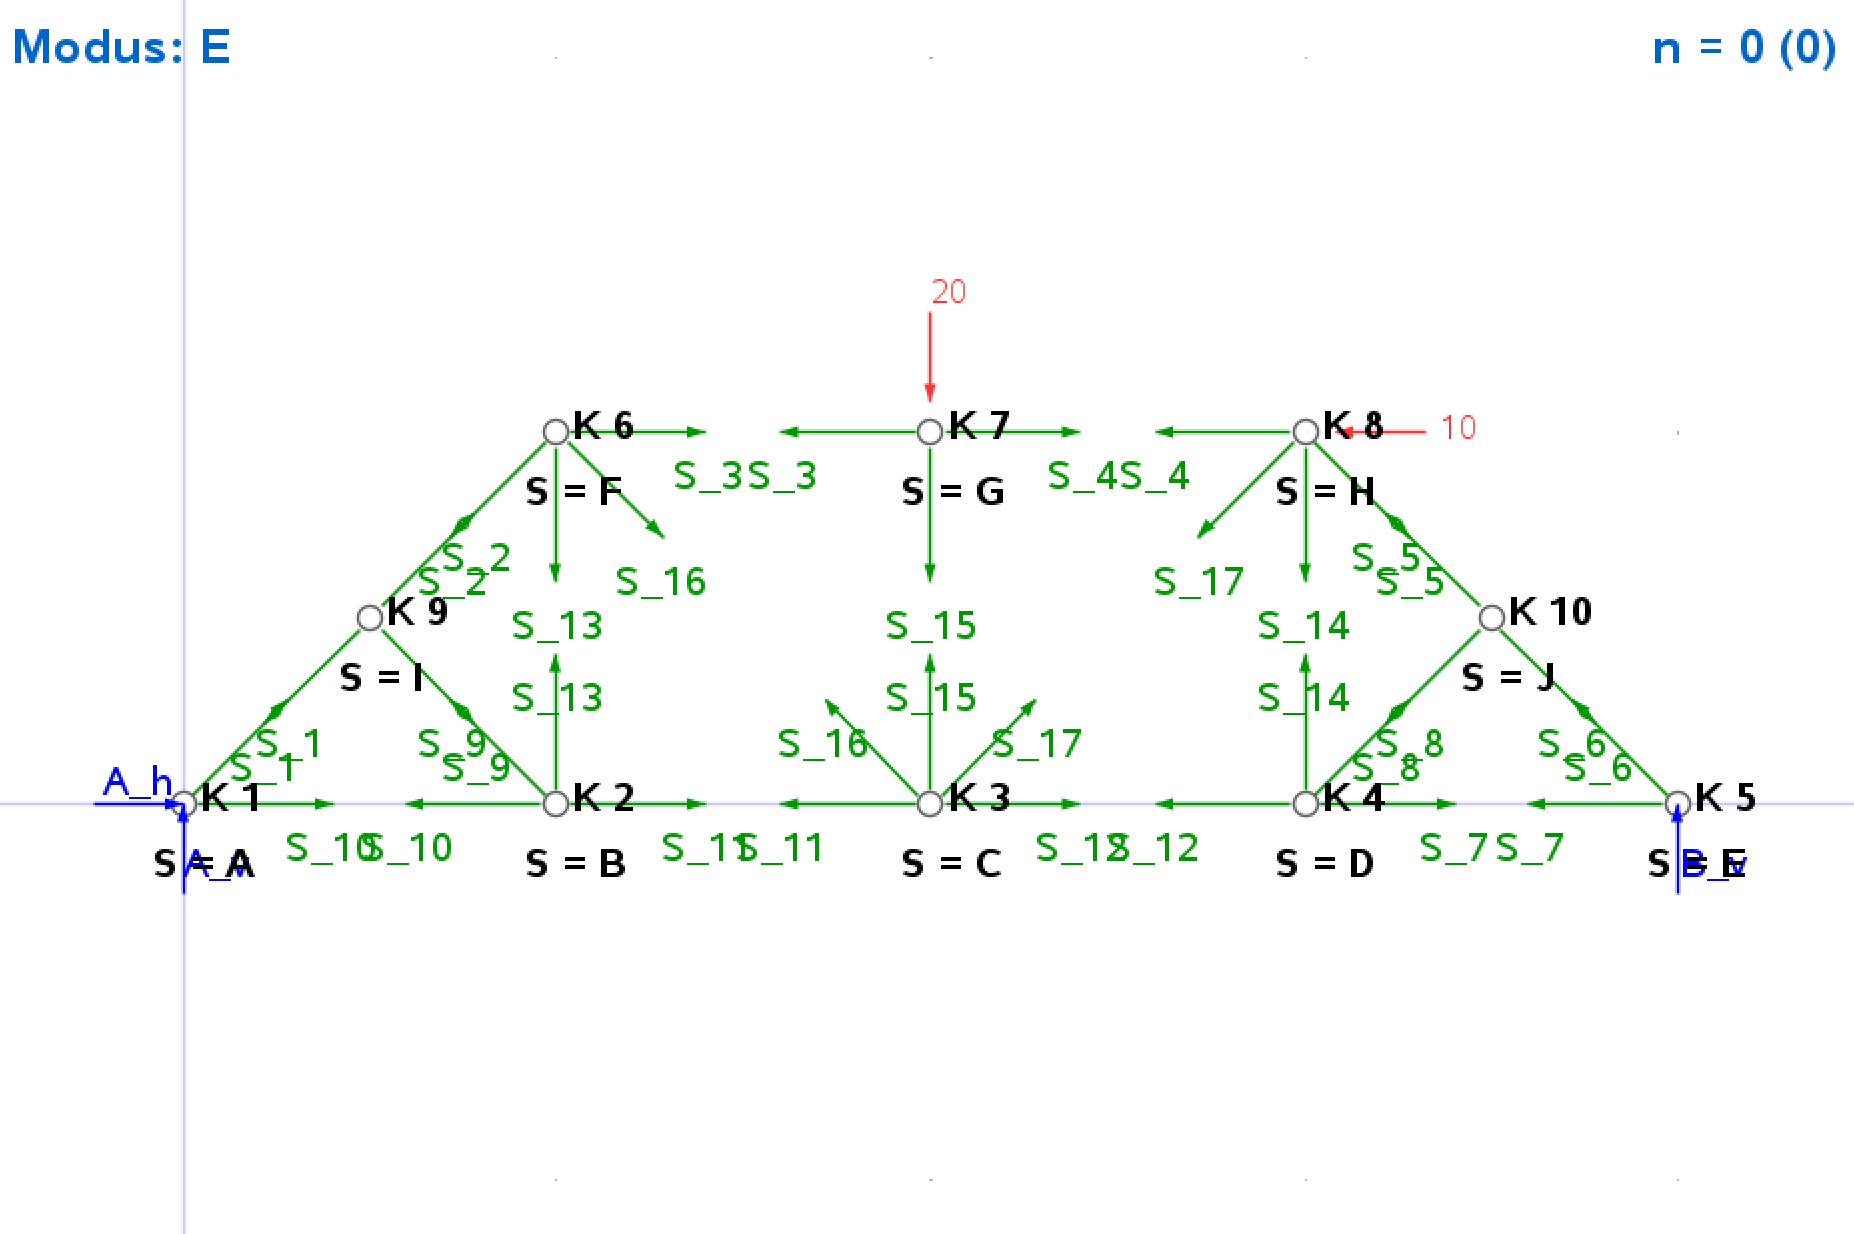
\includegraphics[width=0.5\linewidth]{./fig/TM1/WiSe2122nr6_2.png}
    \caption{TM1 WiSe~21/22 Freischnitt}
    \label{fig:TM1WiSe2122Nr6_2}
\end{figure}

Für die Verwendung der beiden Seiten des E-Modus muss darauf geachtet werden, dass entweder die Stäbe in der
gleichen Reihenfolge wie in der Aufgabe gezeichnet werden oder die Bennenung hinterher angepasst wird. Macht ihr das nicht
ist z.B. Stab 13 aus eurer Rechnung nicht Stab 13 aus der Aufgabe\\
Gleiches gilt natürlich auch für die Verwendung des LGS-Exports. Hier wird (Falls der Fachwerk Modus an ist) 
das Knotenschnittverfahren verwendet. Die Benennung im LGS ist die gleiche wie auf der zweiten Seite des E-Modus.





\section{TM2}

\subsection{Biegelinie (TM2 WiSe~21/22, Nr.~7)} \label{ex:Biegelinienaufgabe}

In dieser Aufgabe ist ein \emph{interessantes} KOS vorgegeben: Soll es ein Rechtssystem sein,
zeigt die $y$-Achse hier in die Zeichenebene hinein und nicht, wie sonst üblich, aus ihr heraus.

Rechnet ihr von Hand über die DGL $EI\,w'''' = q$ mit allen Rand- und Übergangsbedingungen (so
geht man bei statisch unbestimmten Systemen meist vor, und so rechnet auch \code{wneu}), gibt es
hier nichts weiter zu beachten. Bei einem statisch bestimmten System lohnt es sich dagegen, zuerst
die Momentenlinie zu berechnen und dann $EI\,w'' = -M$ zu integrieren. Dafür braucht ihr die
gestrichelte Faser. Die Regel aus Abschnitt~\ref{sec:Eingabe_Stäbe}, dass sie immer auf der Seite
liegt, in die die $z$- bzw.\ $w$-Achse zeigt, gilt auch hier. Alternativ könnt ihr euch überlegen,
auf welcher Seite ein positives Schnittmoment $M_y$ (Drehsinn nach der Rechte-Hand-Regel um die
$y$-Achse) Zug erzeugt, dort liegt die gestrichelte Faser. Das finde ich aber umständlicher.

Im Programm müsst ihr solche Systeme etwas anders eingeben, denn dort zeigt die $y$-Achse immer
aus der Zeichenebene heraus. Zeichnet ihr das System genau wie in der Aufgabe und setzt die
gestrichelte Faser nach der Regel oben, läuft die $x$-Koordinate im Programm in die andere Richtung
als in der Aufgabe. Um das zu umgehen, zeichnet ihr Systeme, bei denen die $y$-Achse in die
Zeichenebene hineinzeigt, spiegelverkehrt (Abb.~\ref{fig:Biegelinienaufgabe}). Ich habe die
Aufgabe im symbolischen Modus gerechnet, deshalb stehen in den Ergebnissen $q$ und $l$.

\begin{figure}[htbp]
    \centering
    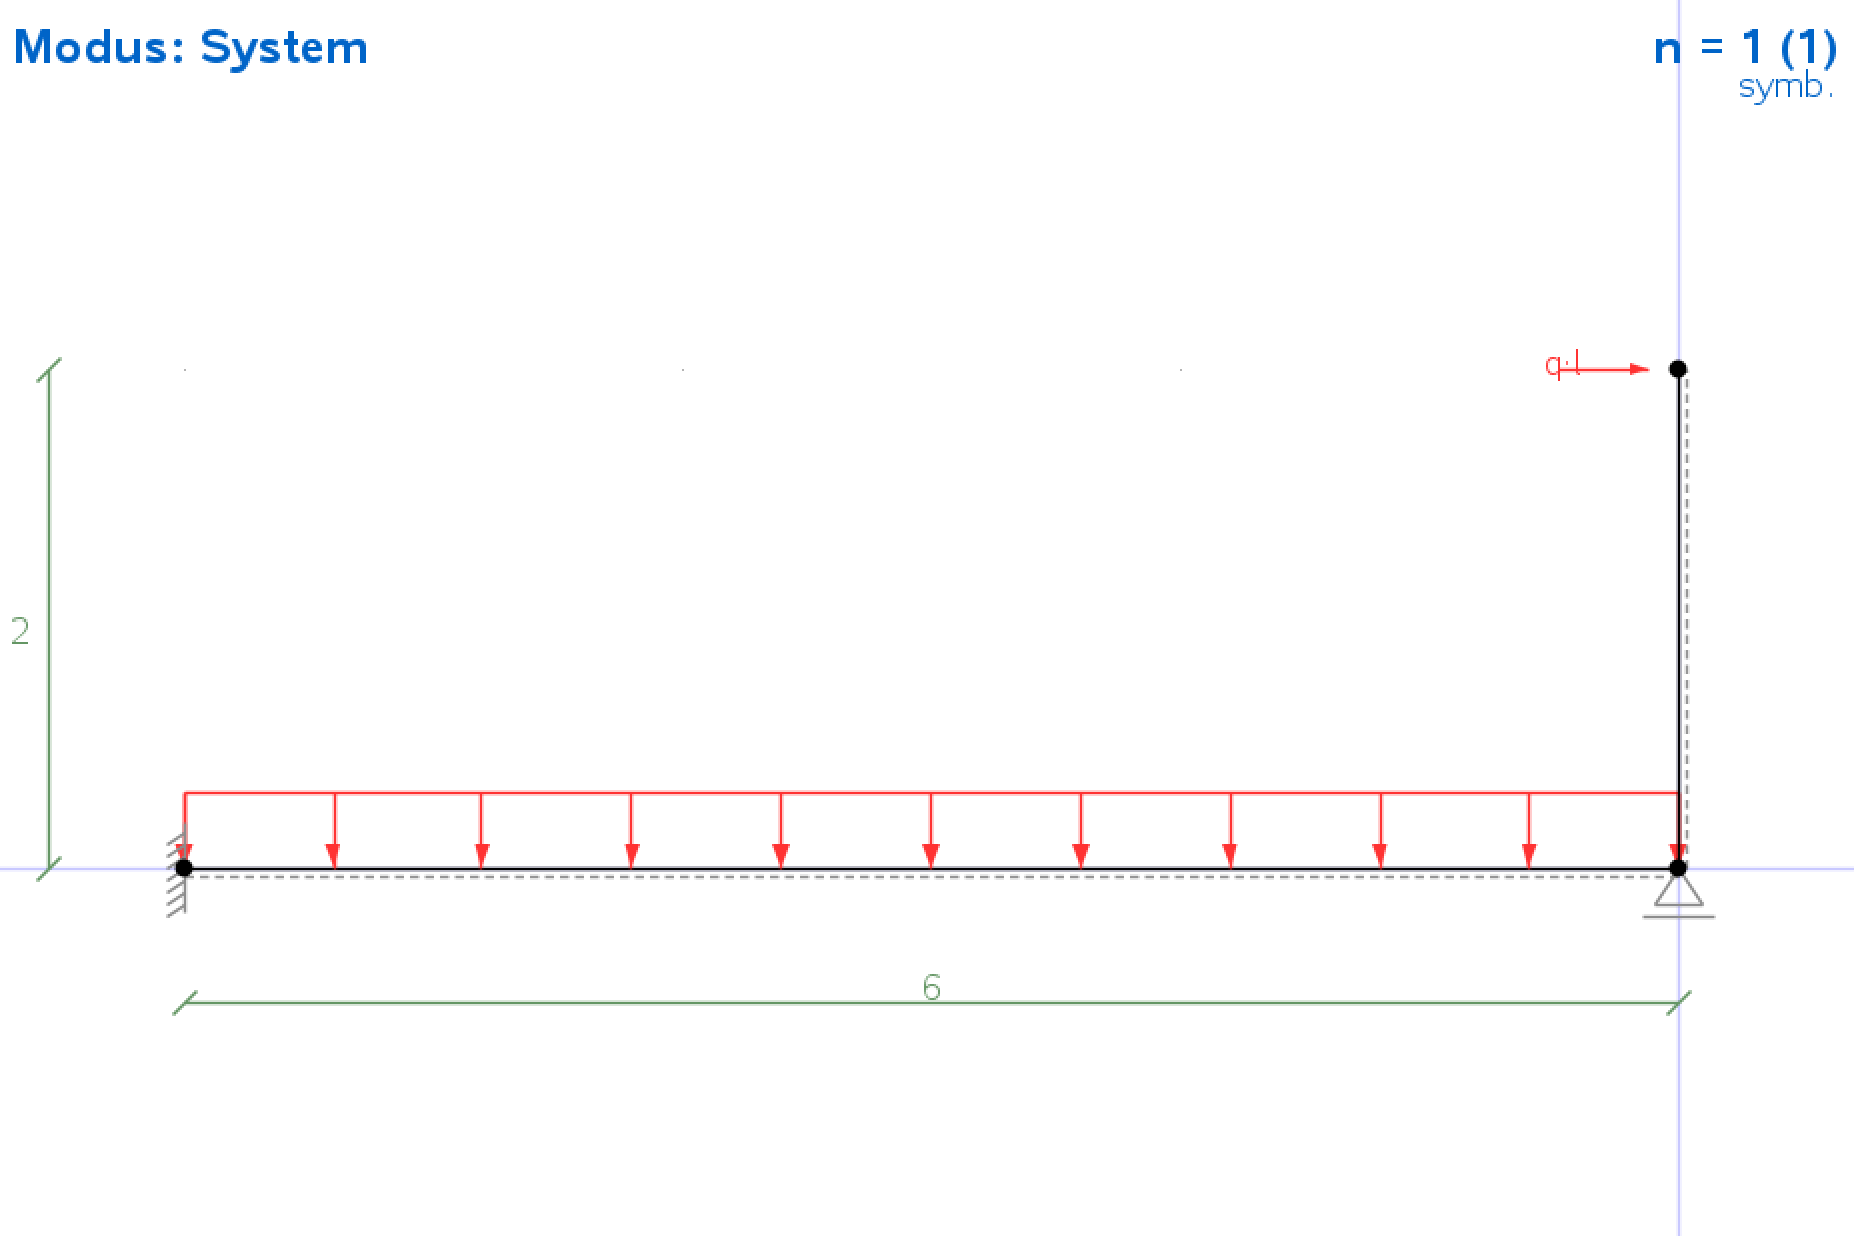
\includegraphics[width=0.5\linewidth]{./fig/TM2/WiSe2122nr7_1.png}
    \caption{TM2 WiSe~21/22, Nr.~7 im Programm, spiegelverkehrt gezeichnet}
    \label{fig:Biegelinienaufgabe}
\end{figure}

Das liefert die Ergebnisse in Abb.~\ref{fig:BiegelinienaufgabeBiegelinie}. Hier geben beide
Methoden dasselbe Ergebnis. Das sollte natürlich so sein, ist aber nicht immer so: Manchmal weicht
die WGV/FEM-Lösung \code{v\_EI\_stab1(x)} (im Rechner klein geschrieben) minimal von der exakten
Lösung \code{wneu1(x)} ab. Weil das Programm die Brüche aus den Zahlen der FEM-Lösung
\emph{errät} (Abschnitt~\ref{sec:mathe-symbolisch}), kann daraus eine ganz anders aussehende
Biegelinie werden. Die Methode über die WGV/FEM-Lösung gibt es trotzdem, vor allem weil ich sie
zuerst programmiert habe (daher wohl auch der Name \code{wneu} der anderen Funktion), und weil sie
bei sehr großen Systemen deutlich schneller sein kann.

\begin{figure}[htbp]
    \centering
    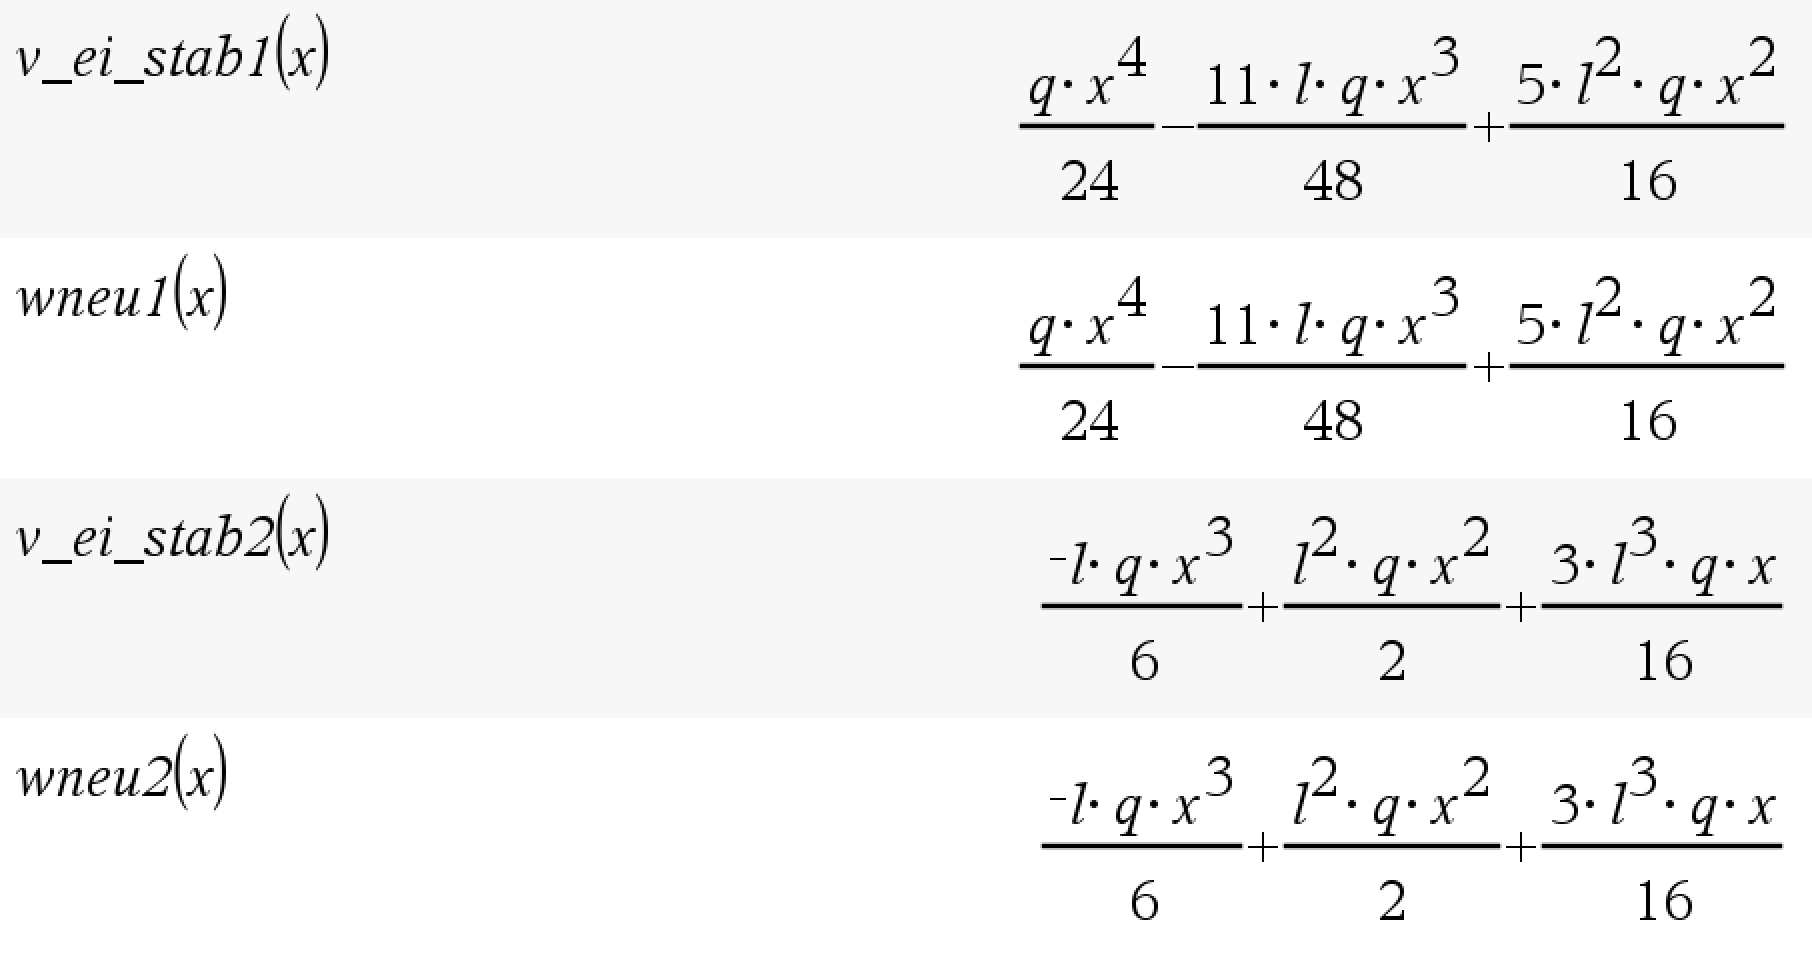
\includegraphics[width=0.5\linewidth]{./fig/TM2/WiSe2122nr7_2.png}
    \caption{TM2 WiSe~21/22, Nr.~7: \code{v\_EI\_stab} und \code{wneu} im Vergleich}
    \label{fig:BiegelinienaufgabeBiegelinie}
\end{figure}

Weil die Stäbe dehnsteif sind, kann das Programm hier sogar die Randbedingungen für Biegelinie und
Längslinie getrennt angeben (Abb.~\ref{fig:BiegelinienaufgabeRandbed}): Die Bedingungen im oberen
Block reichen für die Biegelinie allein, die im unteren kommen nur für die Längslinie dazu. Das geht
nicht immer. Sind die Stäbe dehnbar, hängt die Biegelinie über die Rahmenecken auch von den
Längsverformungen ab, und das Programm gibt alle Bedingungen zusammen aus
(Abschnitt~\ref{sec:randlgs}).

\begin{figure}[htbp]
    \centering
    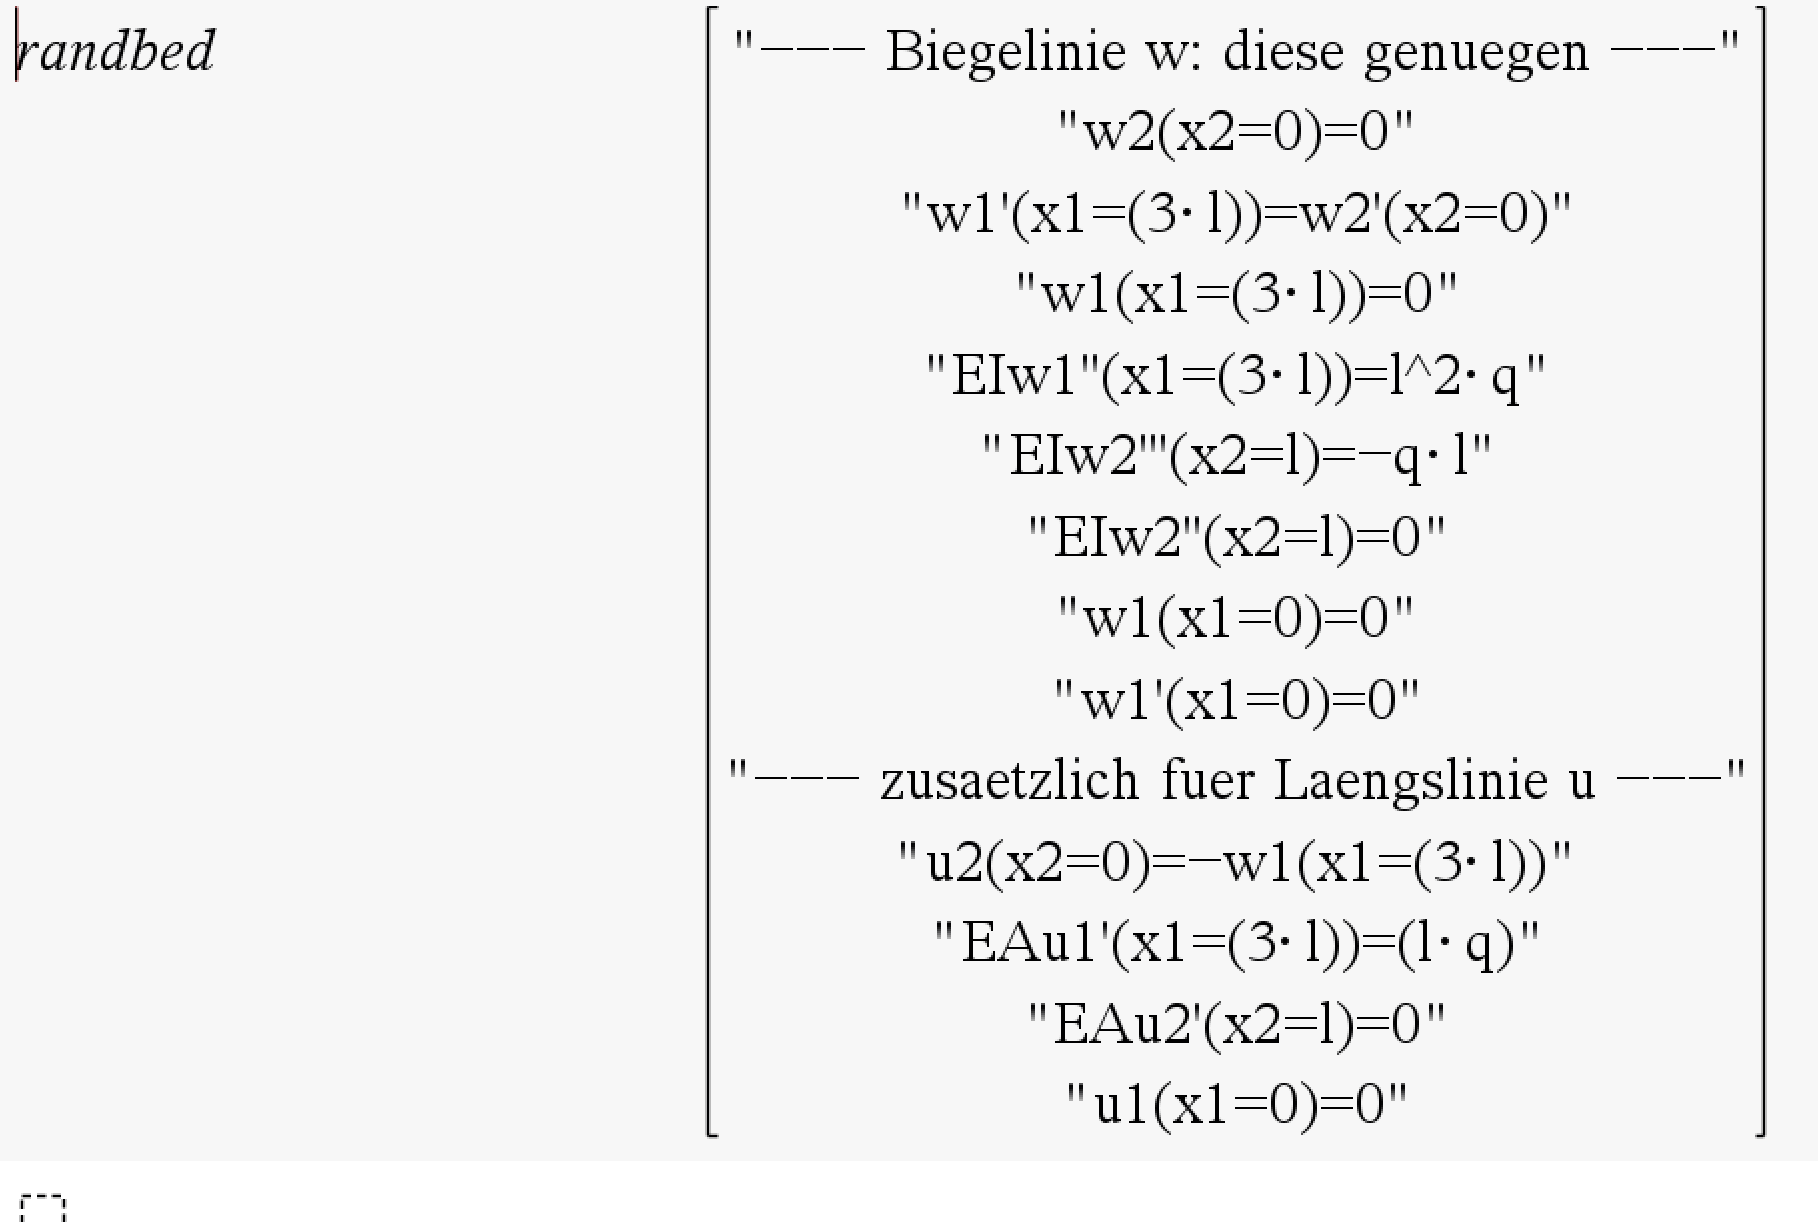
\includegraphics[width=0.5\linewidth]{./fig/TM2/WiSe2122nr7_3.png}
    \caption{Randbedingungen \code{randbed} für TM2 WiSe~21/22, Nr.~7}
    \label{fig:BiegelinienaufgabeRandbed}
\end{figure}



\subsection{Verschiebungsaufgaben (TM2 WiSe~20/21 Nr.~4)} \label{ex:Temperaturaufgabe}

Aufgaben wie diese lassen sich mit der richtigen Eingabe auch direkt im Programm lösen. Wie diese Aufagbe im
Programm aussieht ist in Abb.~\ref{fig:verschiebungSystem} dargestellt. Hierbei muss natürlich auf die Einheiten geachtet werden.
In der Aufgabe sind die relevanten Dehnsteifigkeiten nicht direkt gegeben, genauso wie manche Angaben nicht in der
für das Programm geforderten Einheit sind.\\
Für Kräfte immer kN, genauso wie für die Dehnsteifigkeit $EA$ und die Biegesteifigkeit $EI$ in kNm.  

\begin{figure}[htbp]
    \centering
    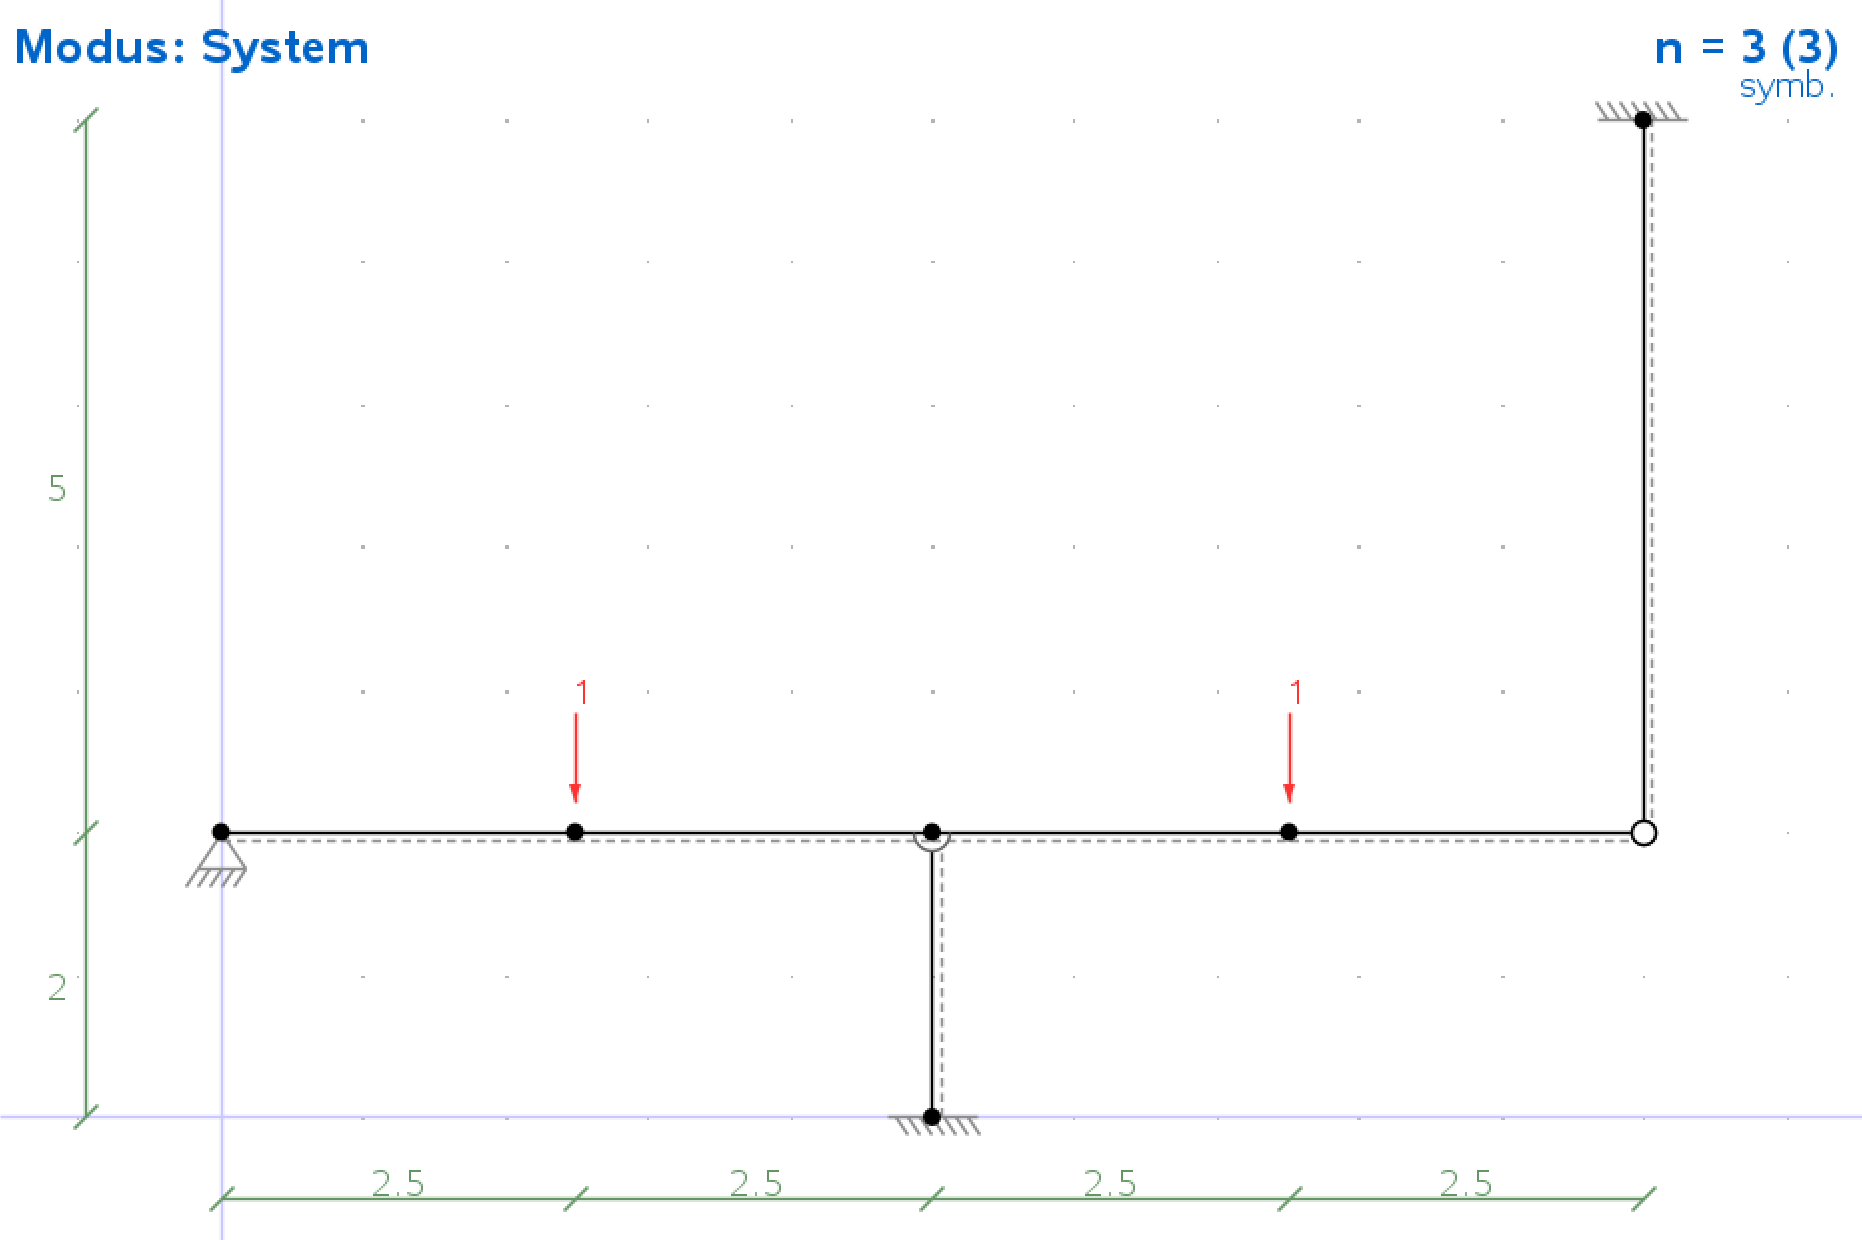
\includegraphics[width=0.5\linewidth]{./fig/TM2/WiSe2021nr4_1.png}
    \caption{TM2 WiSe~20/21, Nr.~4a im Programm}
    \label{fig:verschiebungSystem}
\end{figure}

In den \emph{neuen} Exportfunktionen wird die Temperatur auch symbolisch miteinberechnet.
Um also ann die Verschiebung des rechten unteren Knoten zu kommen lässt sich das entweder über die obere
Knotenexportfunktion machen, über die Biegelinie des rechten horizontalen Stabes oder über die Längsverschiebungsfunktion
des rechten vertikalen Stabes. Über den CAS Befehl \code{solve()} lässt sich die Temperatur direkt ausrechnen 
(vgl. Abb.~\ref{fig:verschiebungErgebniss}). Ich habe hier die Tempertur $dt$ genant (nur $T$ ist wie bereits erwähnt nicht erlaubt),
die Variable nach der aufgelöst werden soll muss der \code{solve()} Funktion als zweites Argument mit gegeben werden.

\begin{figure}[htbp]
    \centering
    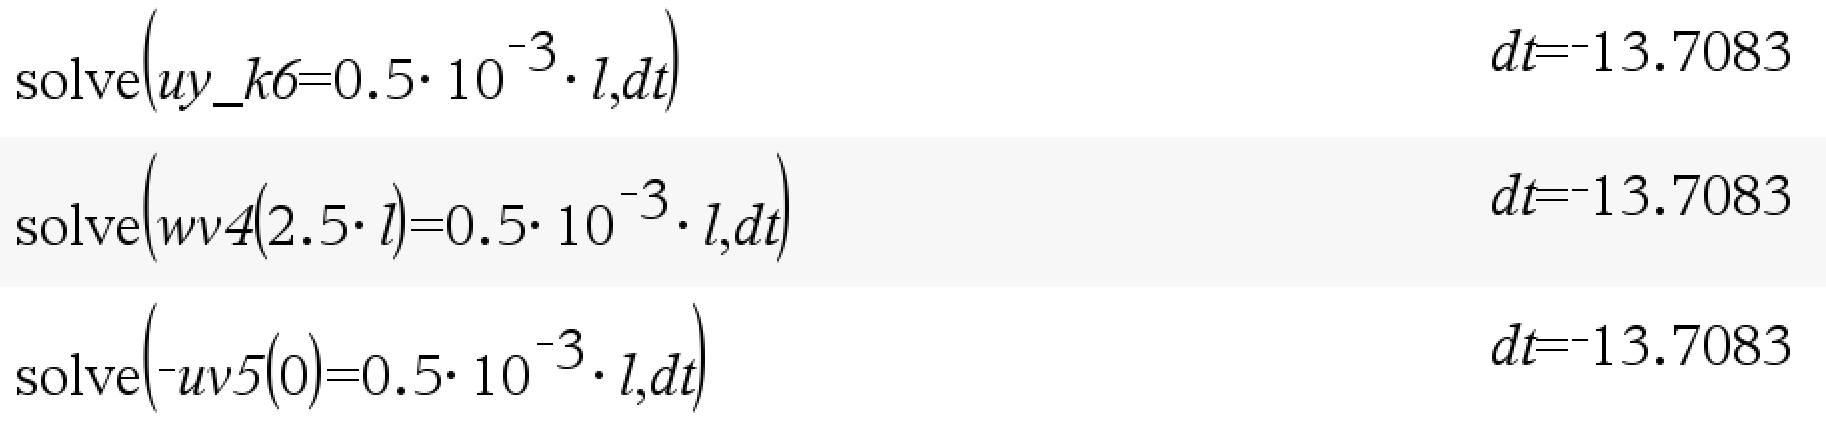
\includegraphics[width=0.5\linewidth]{./fig/TM2/WiSe2021nr4_2.png}
    \caption{Lösung von TM2 WiSe~20/21, Nr.~4a}
    \label{fig:verschiebungErgebniss}
\end{figure}

Der Zweite Teil der Aufgabe lässt sich auch im Programm lösen (Abb.~\ref{fig:VerschiebungTemp}), jedoch gibt es auch hier
ein paar Feinheiten. Ein deratiges System zu speichern kann sich lohnen. Auch hier gelten natürlich die gleichen Hinweise zu den Einheiten.

\begin{figure}[htbp]
    \centering
    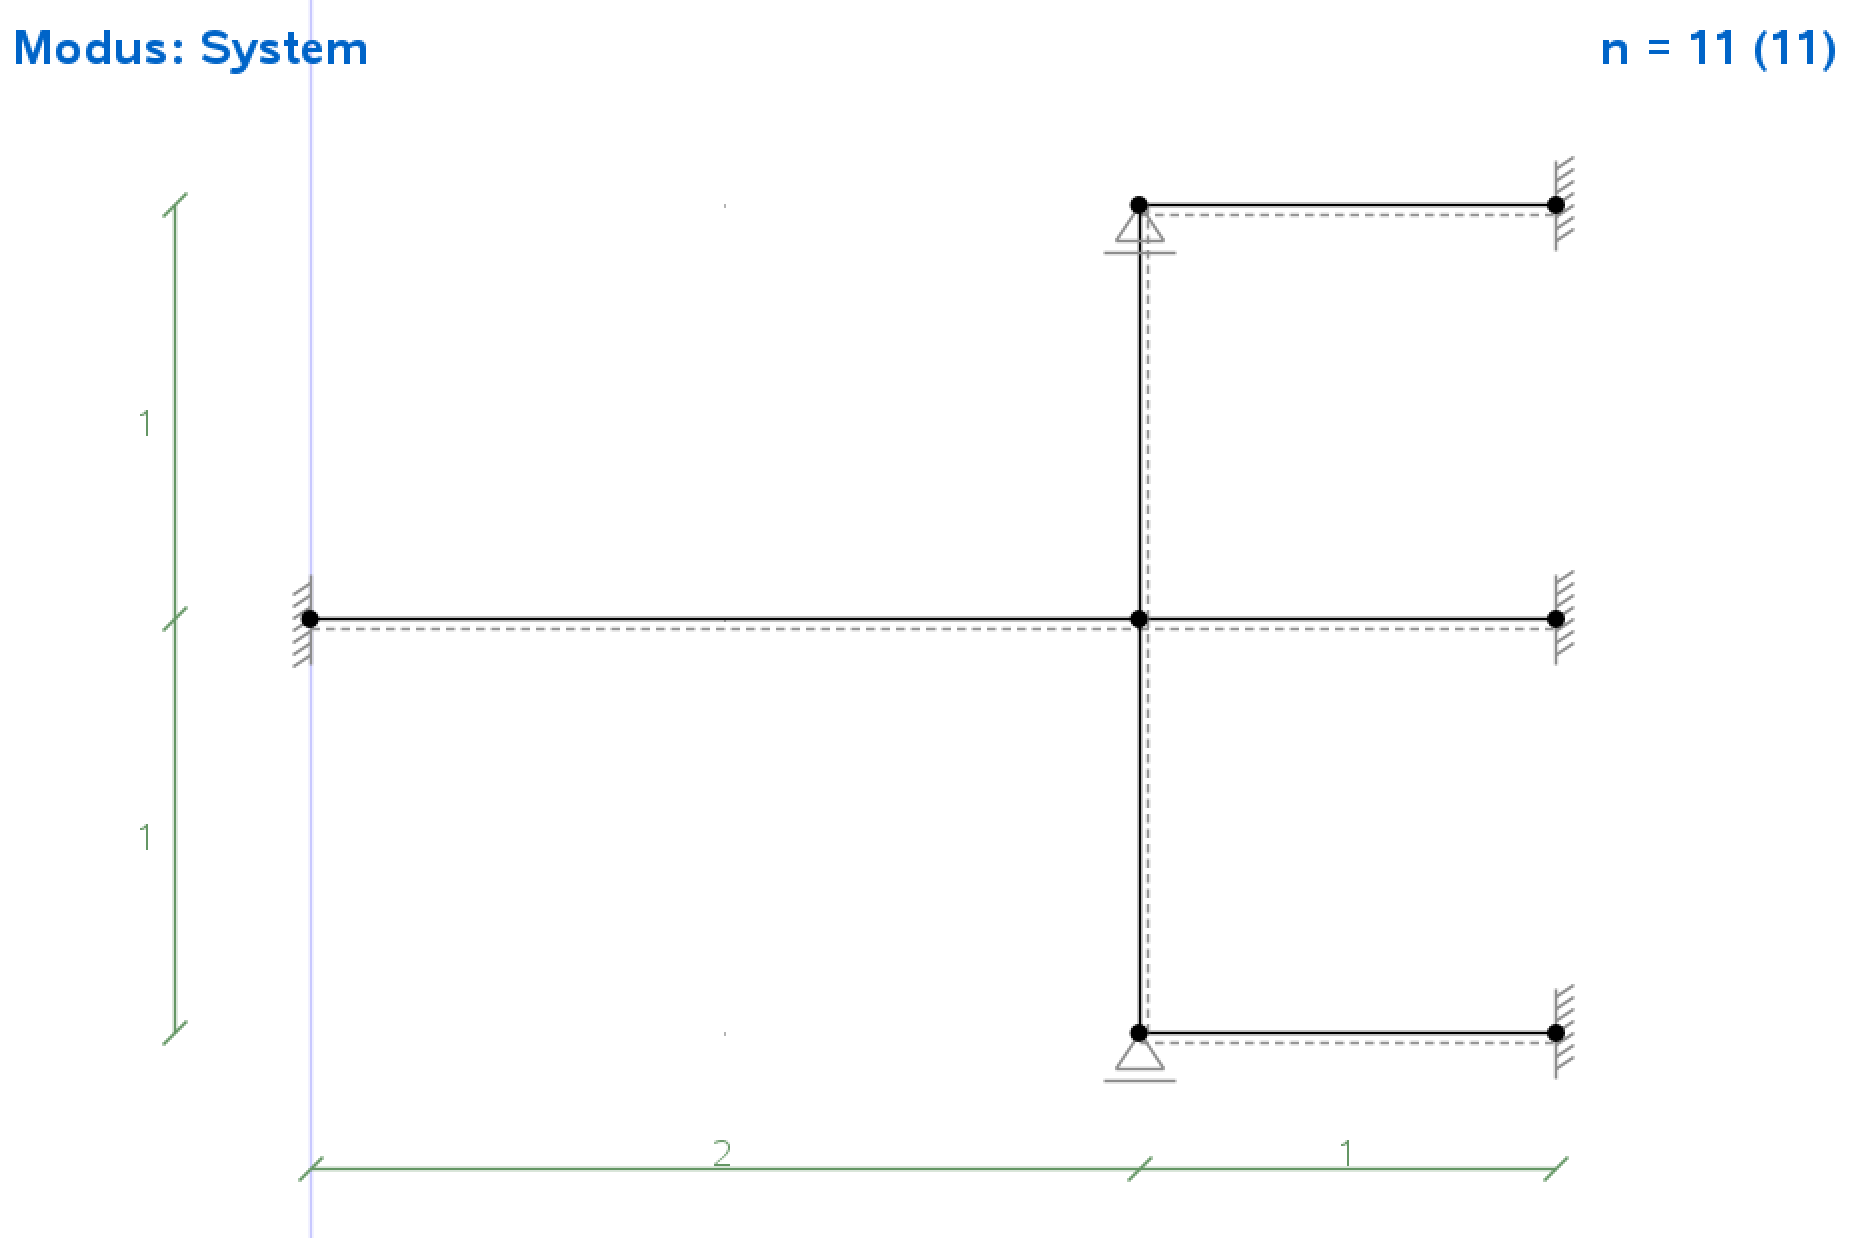
\includegraphics[width=0.5\linewidth]{./fig/TM2/WiSe2021nr4_3.png}
    \caption{TM2 WiSe~20/21, Nr.~4b im Programm}
    \label{fig:VerschiebungTemp}
\end{figure}

Da das Programm nur schnittgrößen direkt berechnet müssen diese noch in Spannungen umgerechnet werden, dafür gibt es in diesem Fall
zwei Möglichkeiten (vgl. Abb.\ref{fig:TM2WiSe2021Nr4b}). Entweder man rechnet die Spannunge direkt über die Schnittkraftverläufe aus,
oder über die Ableitung der Verschiebungsfunktion. Für die zweite Methode muss jedoch darauf geachtet werden den Temperatur Anteil
korrekt zu verrechnen.\\
Erstere Methode ist für Aufgaben mit Zahlenwerten auf jeden Fall die Einfachere, für Aufgaben mit symbolischen Temperatur Werten muss jedoch
die zweite Methode gewählt werden, da die Schnittkraftverläufe diese nicht auf die gewünschte Art berücksichtigen.

\begin{figure}[htbp]
    \centering
    \begin{subfigure}[t]{0.48\textwidth}
        \centering
        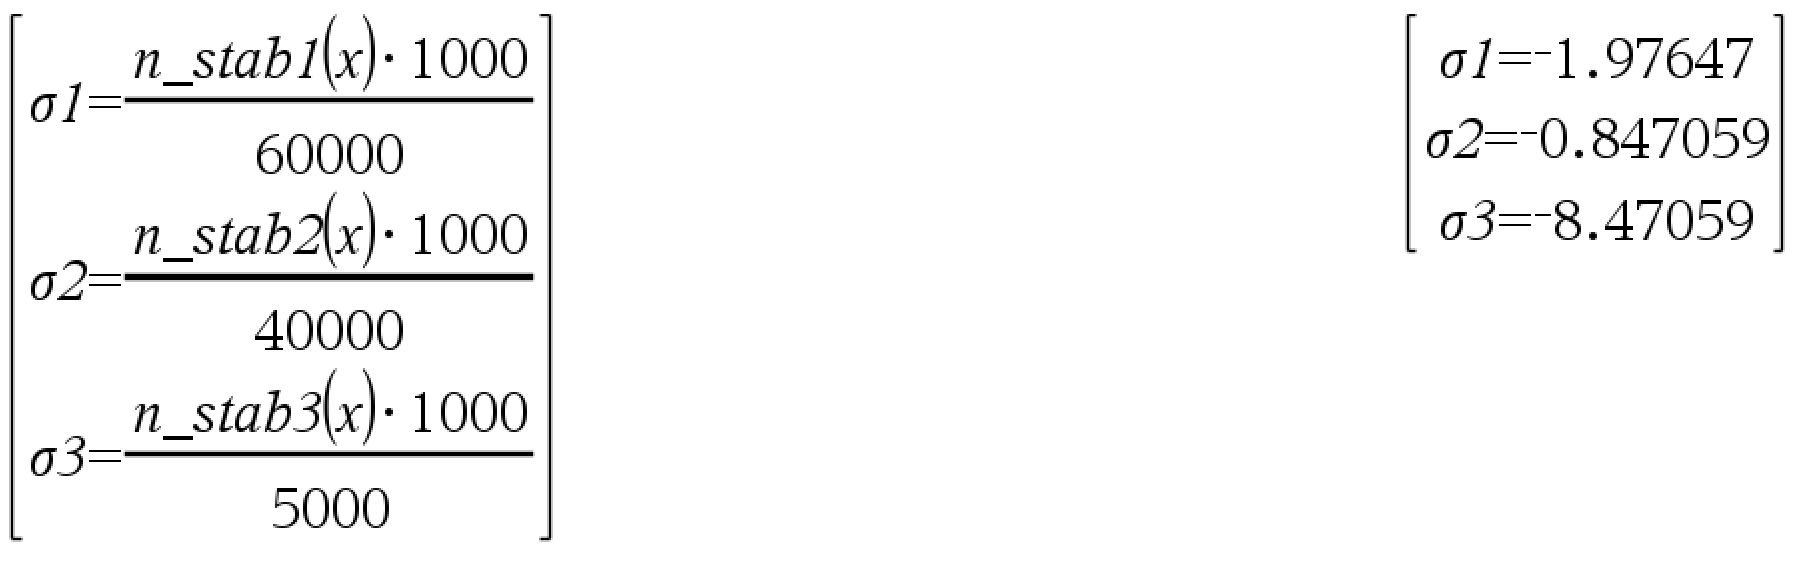
\includegraphics[width=\linewidth]{./fig/TM2/WiSe2021nr4_4.png}
        \caption{Über Schnittgrößen}
    \end{subfigure}
    \hfill
    \begin{subfigure}[t]{0.48\textwidth}
        \centering
        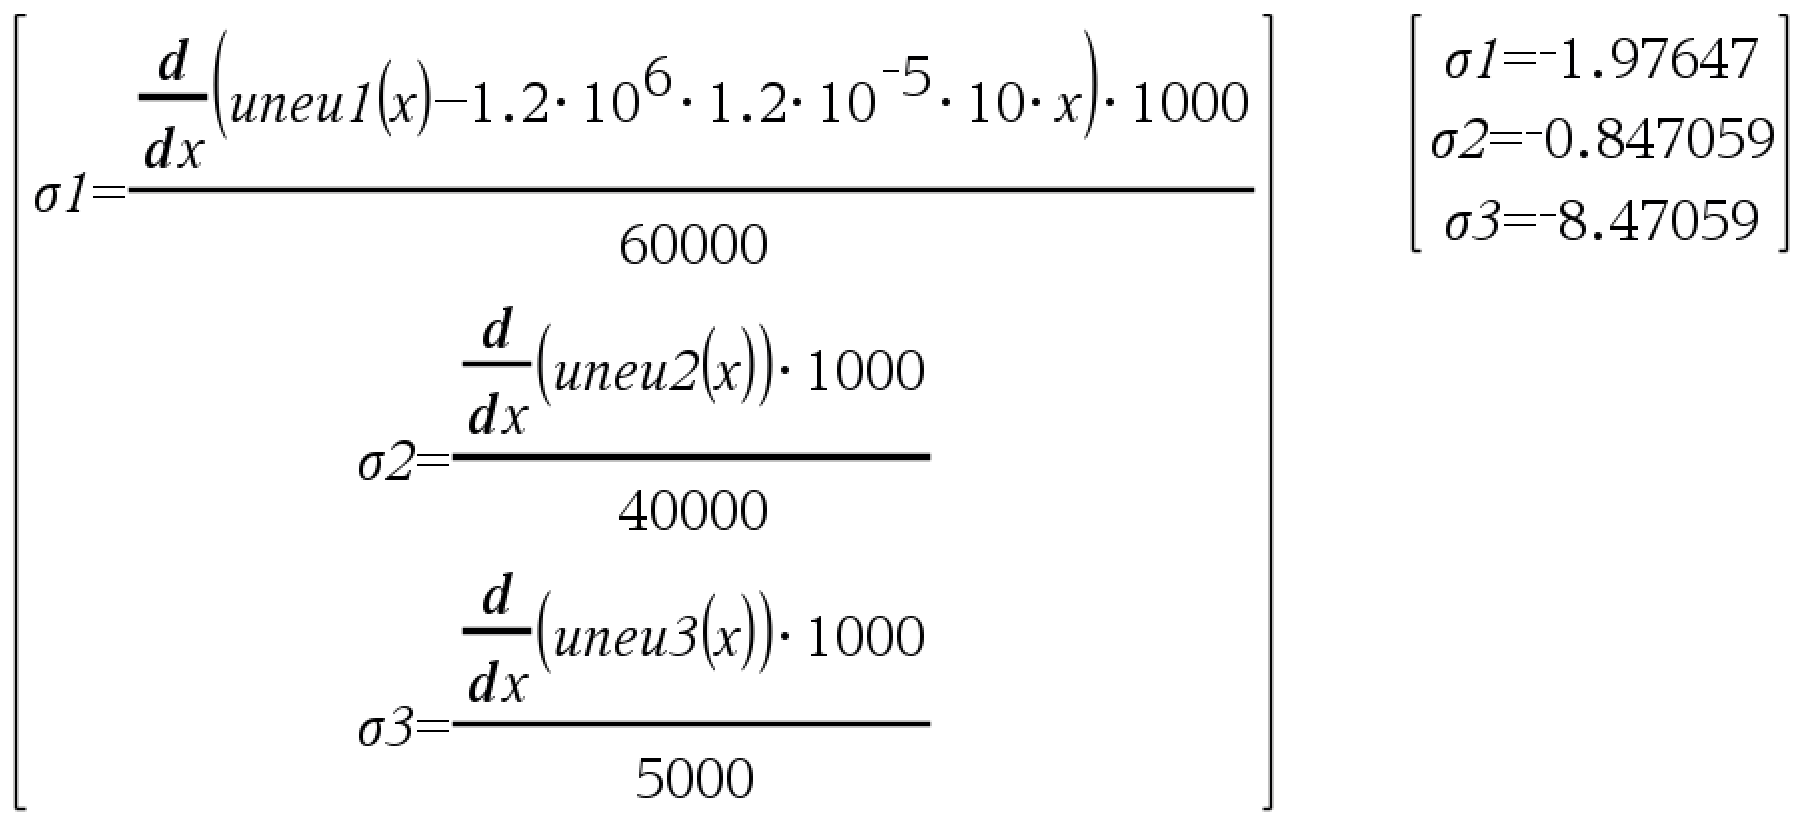
\includegraphics[width=\linewidth]{./fig/TM2/WiSe2021nr4_5.png}
        \caption{Über Verschiebungsfunktion}
    \end{subfigure}
    \caption{Lösung von TM2 WiSe~20/21, Nr.~4b}
    \label{fig:TM2WiSe2021Nr4b}
\end{figure}

Ich will hier anmerken das bei dieser Aufgabenart häufig Hinweise und Warnungen angezeigt werden. Wie z.B. hier auch bei Teilaufgabe a) eine Warnung
zur symbolischen Temperatur. Diese Warnungen sind zwar so konzipiert, dass sie nur angezeigt werden wenn das Programm bzw. ich denke
das etwas falsch eingegeben wurde, jedoch ist es schwer dabei zu vermeiden das auch bei richtiger Eingabe nie eine Warnung oder Hinweis kommt.
Aus diesem Grund empfehele ich, wenn nicht direkt ersichlich ist warum eine Warnung kommt die komplette Eingabe nochmal zu prüfen,
falls diese aber wirklicht korrekt ist sollten auch die Ergebnisse stimmen.


\subsection{Pendelstabannahme (TM2 WiSe 22/23 Nr.~4)} \label{ex:Pendelstabannahme}

\begin{figure}[htbp]
    \centering
    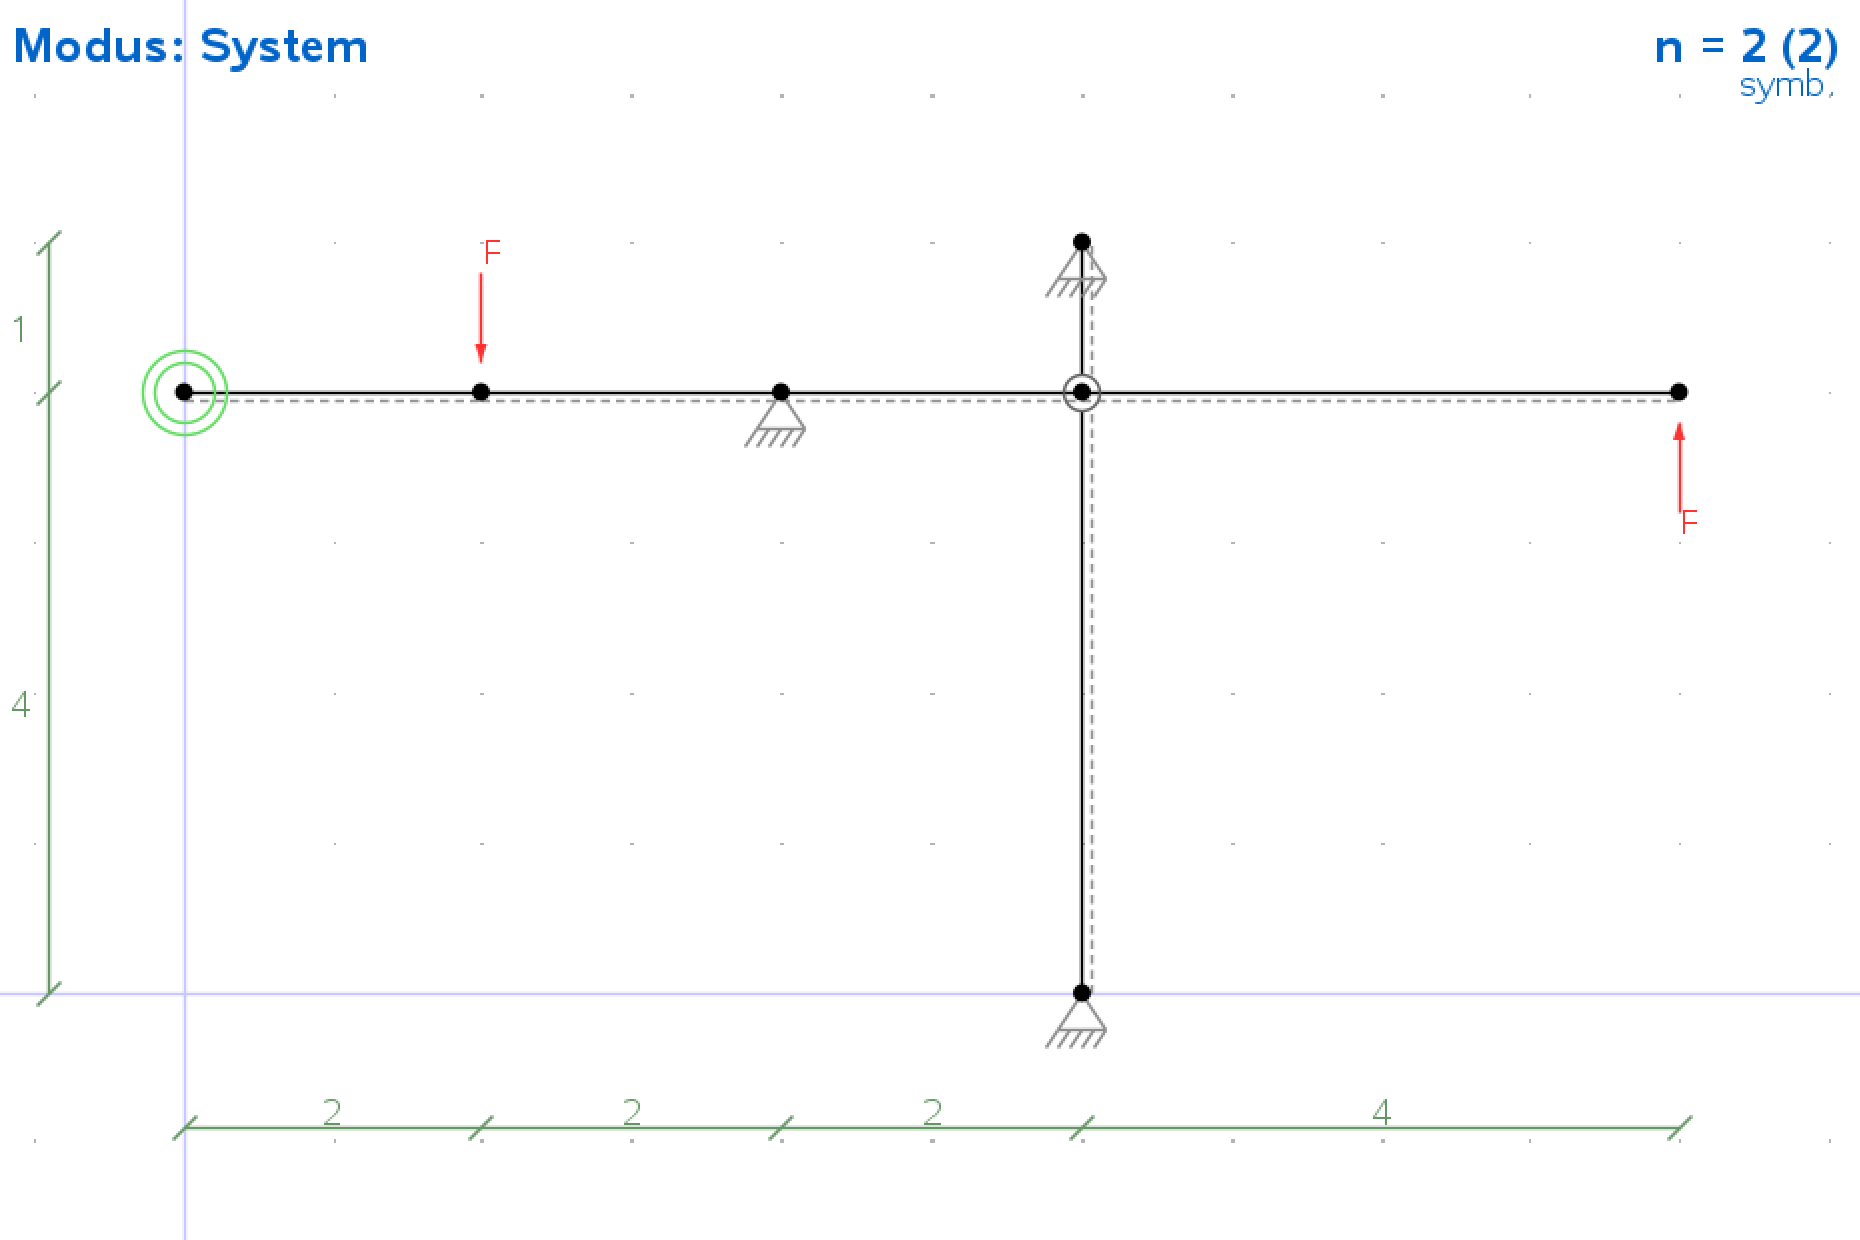
\includegraphics[width=0.7\linewidth]{./fig/TM2/WiSe2223nr4_1.png}
    \caption{TM2 WiSe~22/23, Nr.~4 im Programm}
    \label{fig:Pendelstabsnnahme}
\end{figure}

Wie die Überschrifft vielleicht bereits vermuten lässt muss bei dieser Aufgabe eine Annahme getroffen werden,
die der Zeichnung strenggenommen wiederspricht. Die beiden vertikalen stäbe sollten eigentlich mit einem Angelenk
an den starren Stab angeschlossen werden.\\
Bei einer Handrechnung wird diese Annahme quasi automatisch getroffen, das Programm macht sowas natürlich nicht automatisch.
Um diese Aufgabe mit dem Programm also korrekt zu rechnen müsseb bei den beiden vertikalen stäbe jeweils Angelenke eingebaut werden.
Falls man das nicht macht wirft das Programm eine Warnung bzw. einen Hinweis.

Bei dieser Aufgabe lassen sich die Ergebnisse entweder aus der Ansicht zur Normalkraft 
oder aus dem E-Modus holen (Abb.~\ref{fig:TM2WiSe2223Nr4}).

\begin{figure}[htbp]
    \centering
    \begin{subfigure}[t]{0.48\textwidth}
        \centering
        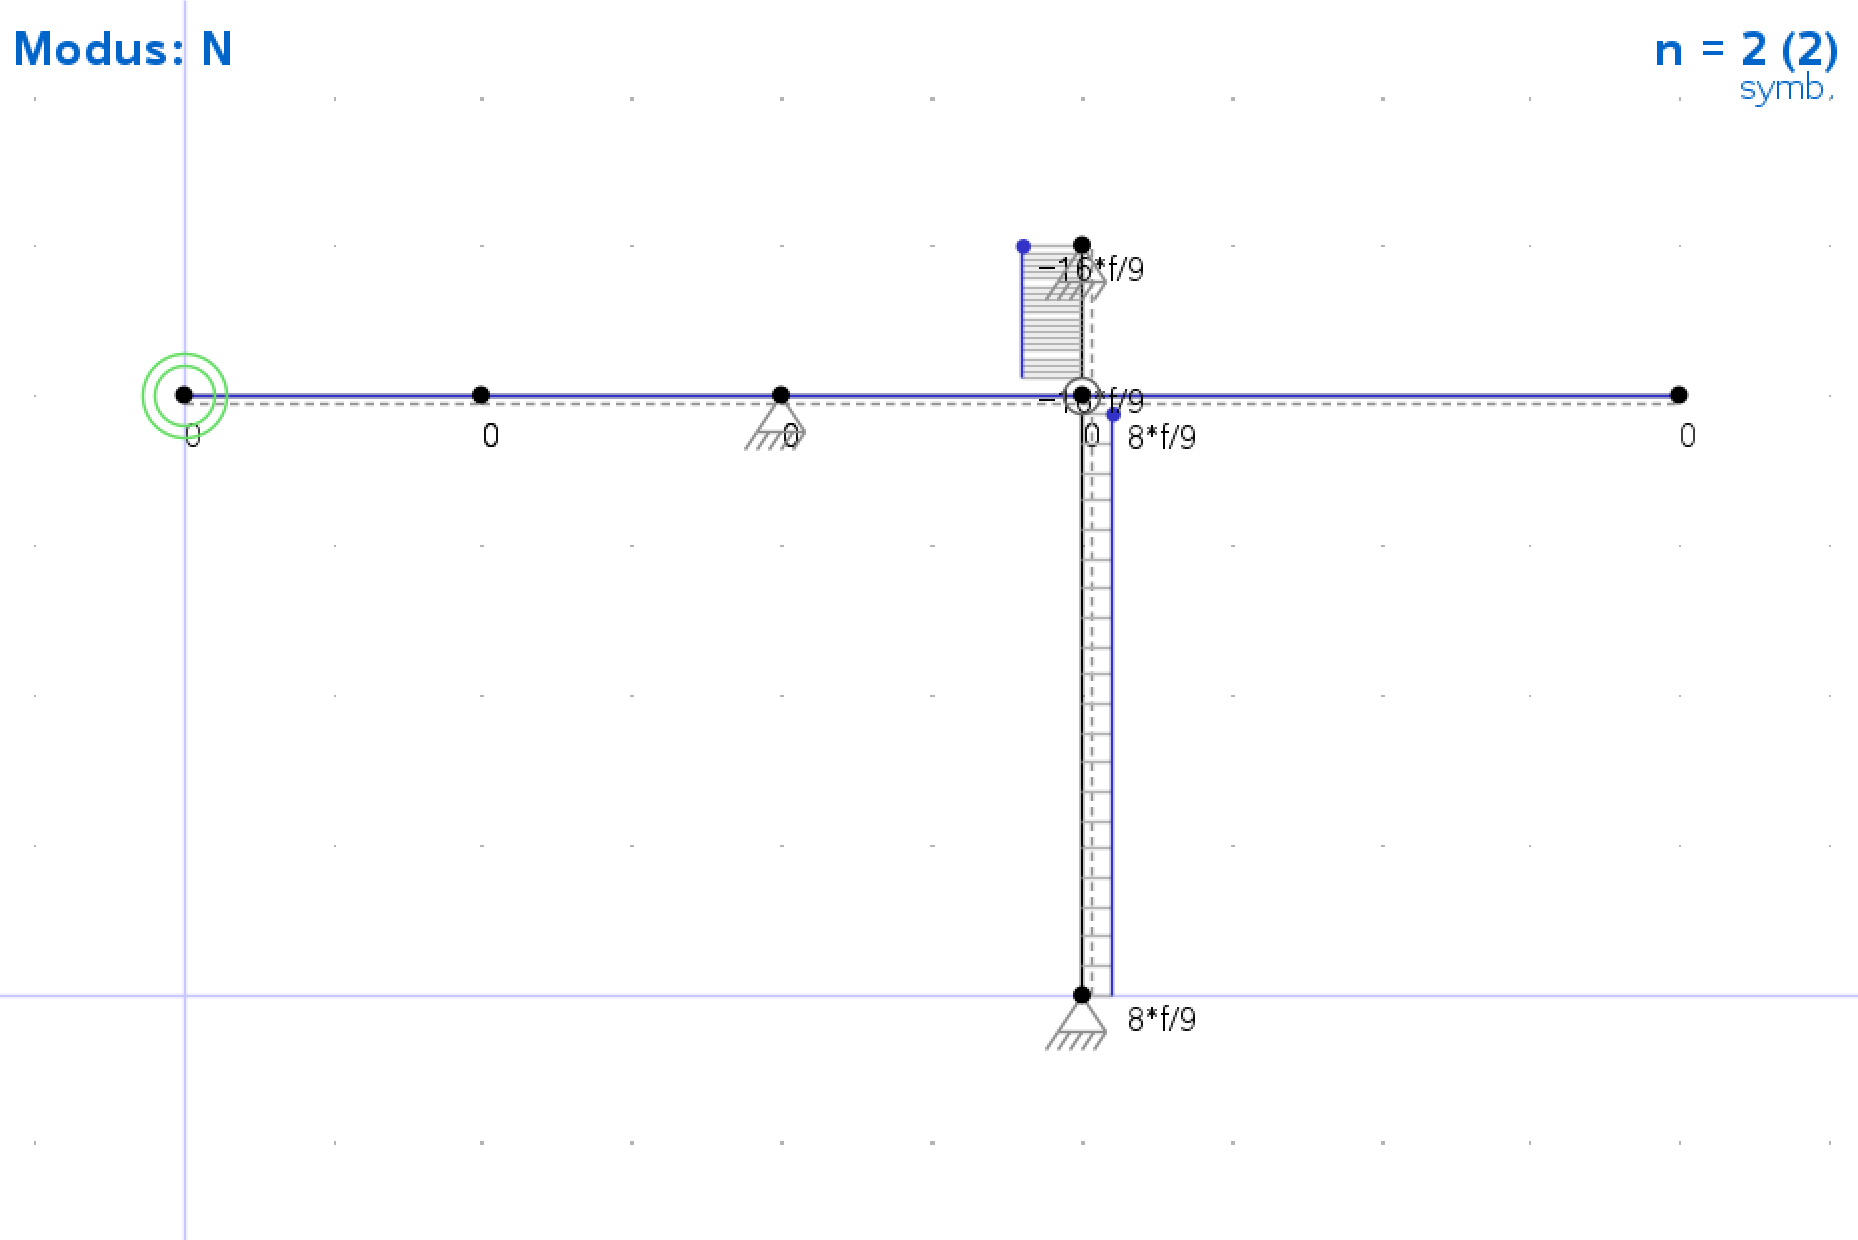
\includegraphics[width=\linewidth]{./fig/TM2/WiSe2223nr4_2.png}
        \caption{Normalkraft}
    \end{subfigure}
    \hfill
    \begin{subfigure}[t]{0.48\textwidth}
        \centering
        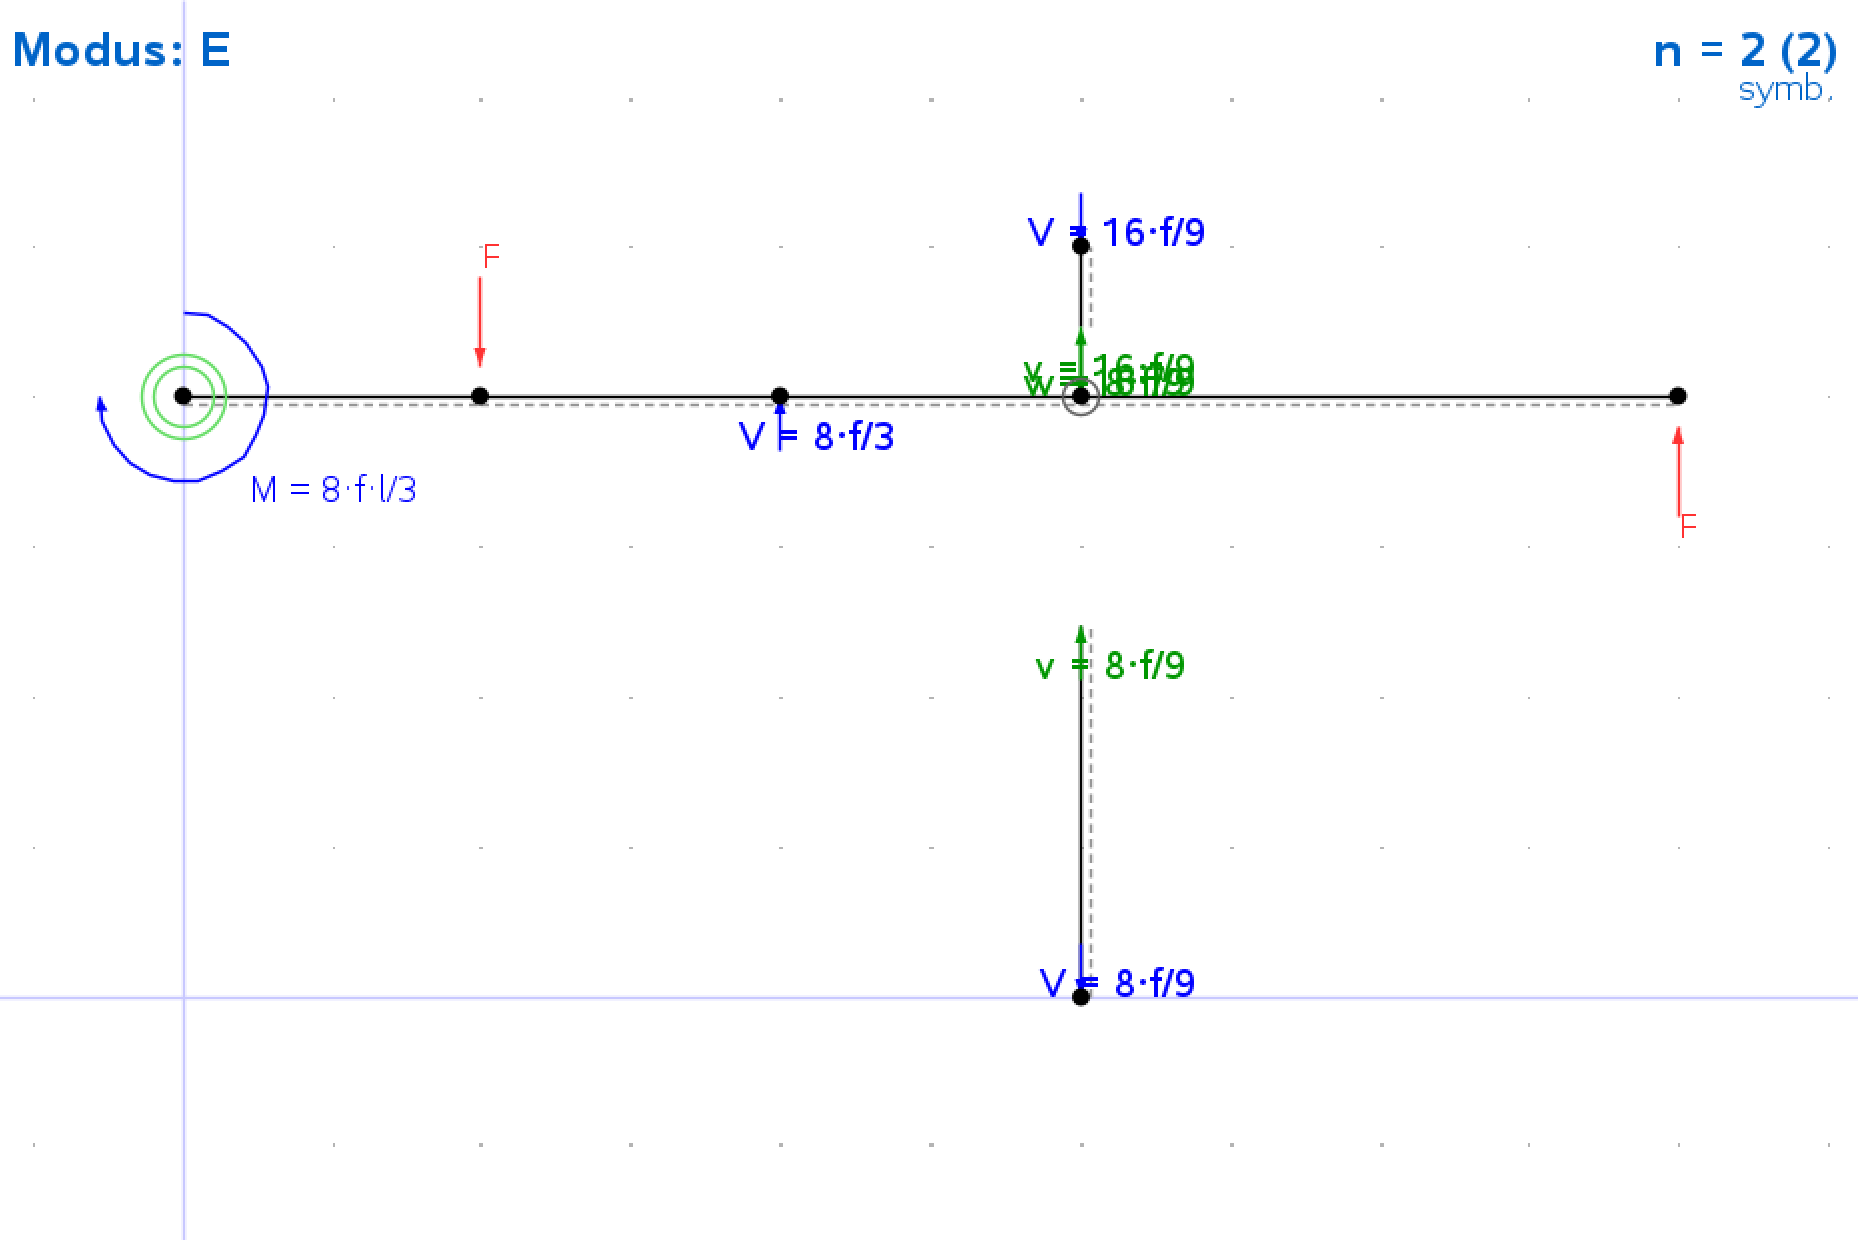
\includegraphics[width=\linewidth]{./fig/TM2/WiSe2223nr4_3.png}
        \caption{E-Modus}
    \end{subfigure}
    \caption{Lösung von TM2 WiSe~22/23, Nr.~4}
    \label{fig:TM2WiSe2223Nr4}
\end{figure}

\textbf{Wichtig} ist, dass das Programm, für symbolische Federn in den Verläufen in seltenen Fällen nicht die richtigen 
Werte ausgibt (Bei symbolischen Temperaturen sowieso nicht).
Zur Sicherheit würde ich deswegen die Schnittgrößen über die \emph{neuen} Verschiebungsfunktionen ermitteln. 
Das dauert zwar gerade für große Systeme länger, ist aber zuverlässiger weil dort wirklich alles symbolisch gerechnet wird 
und eben nicht gepfuscht wird.



\subsection{Schiefe Biegung (TM2 WiSe 25/26 Nr.~8)}

In dieser Aufgbabe sind die Dicken der dünnwandigen Elemente nicht gegeben, da diese abber sowohl für das
FTM als auch für die Lange des Schwerpunkts wichtig sind, müssen diese Werte manuell mit den Werten aus der 
Aufgabenstellung überschrieben werden. Das geht im Obermenue (Taste \taste{o}) auf Seite 3.\\
Für das Zeichnen so eines schiefen Querschnitts empfielt sich ein Rastermaß von z.B. $\frac{1}{\sqrt{2}}$.

\begin{figure}[htbp]
    \centering
    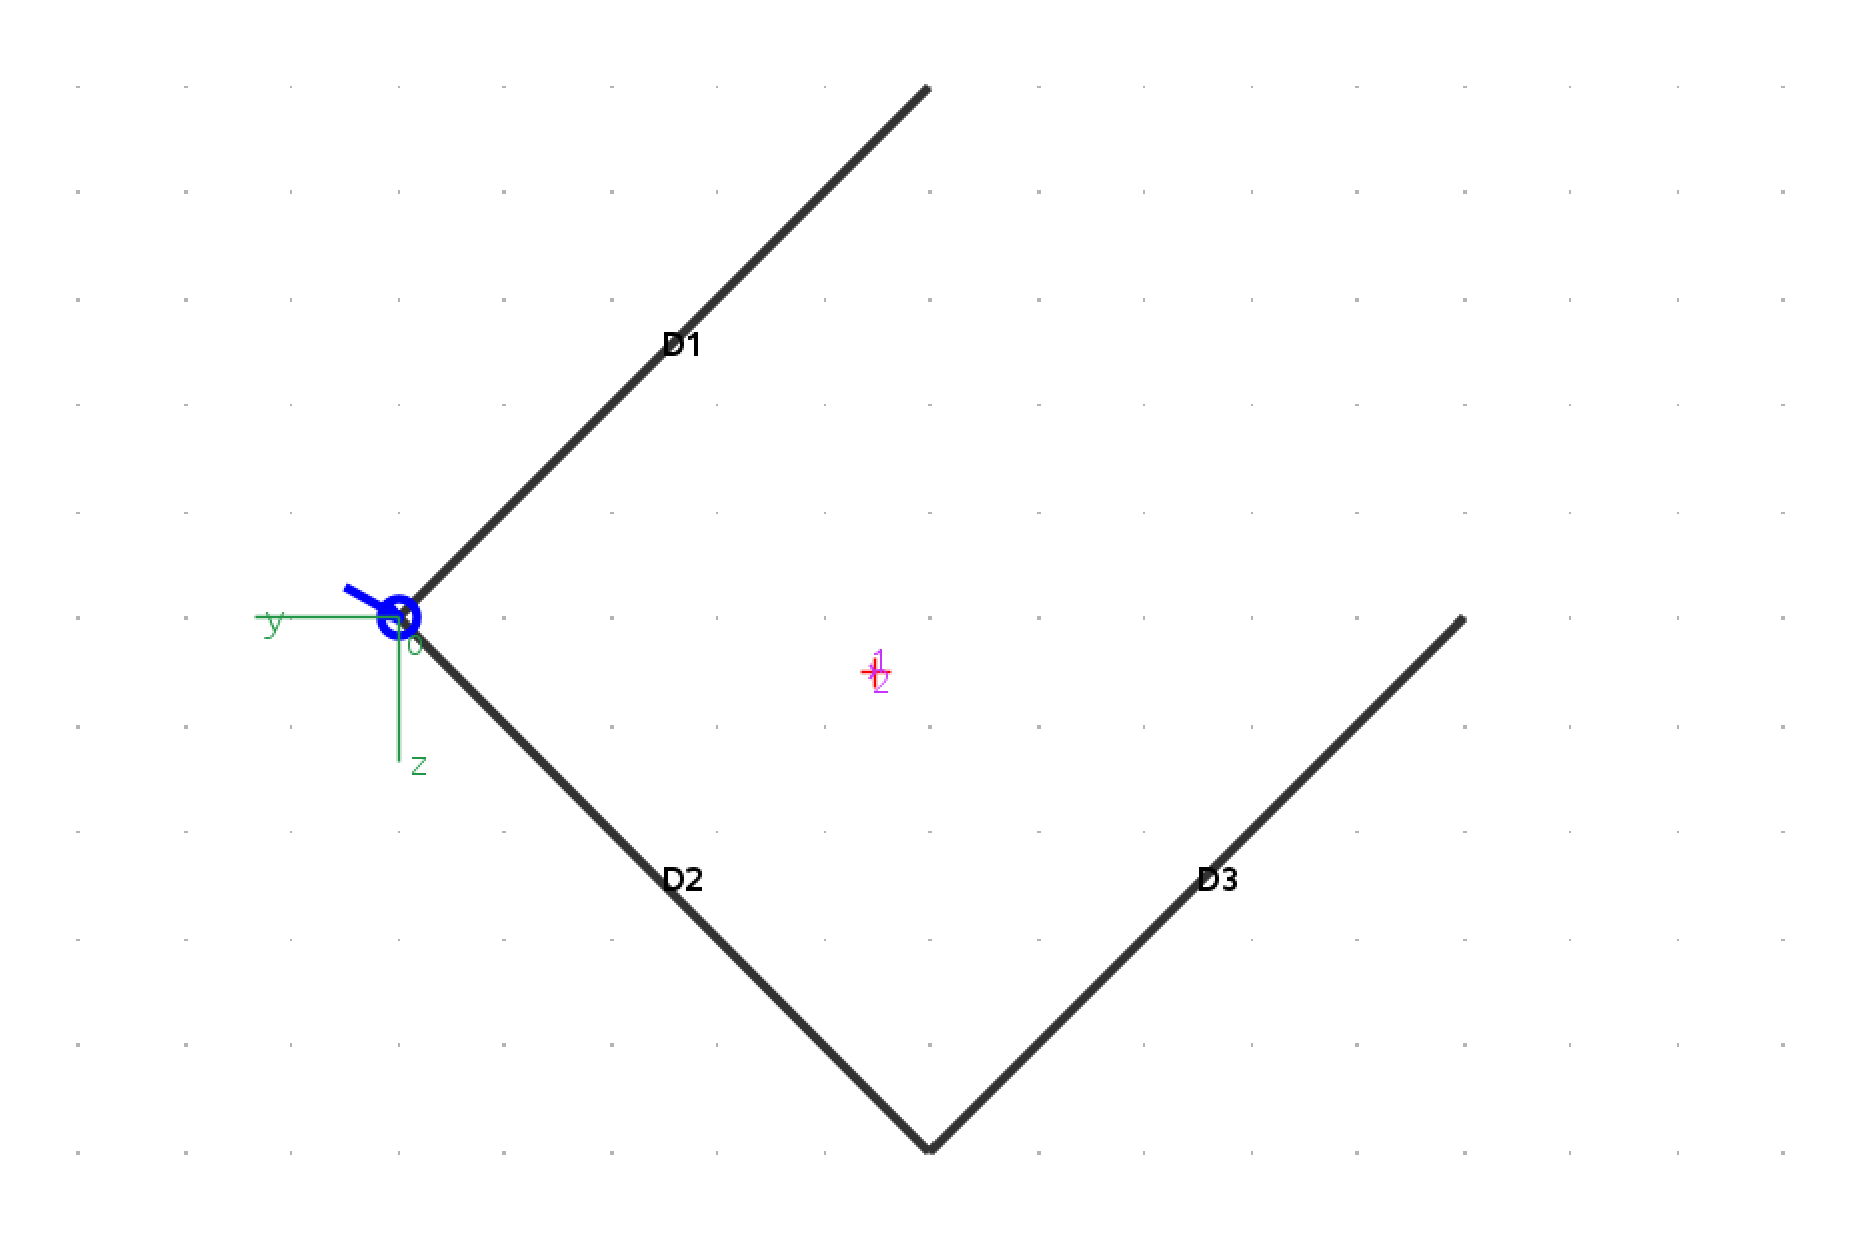
\includegraphics[width=0.7\linewidth]{./fig/TM2/WiSe2526nr8_1.png}
    \caption{TM2 WiSe~25/26, Nr.~8 im Programm}
    \label{fig:TM2WiSe2526Nr8_1}
\end{figure}

Bei dieser Aufgabe braucht man die $\sigma_x$-Berechnung. Um die Normalkraft hier richtig einzuberechnen
muss die Resultierende der Streckenlast über die halbe Länge berechnet werden, also: 
$R=0,1~\frac{\text{kN}}{cm}\cdot100~\text{cm}$.
Für die Kraft muss also $F_y=-500~\text{N}$, $F_z=300~\text{N}$ und $F_x=10000~\text{N}$ eingegeben werden.

Nach dem Aufruf der Berechnung werden noch ein paar Werte abgefragt. Für die ersten Drei muss Null eingetragen werden.
Man hätte auch keine Kraft platzieren können, die Normalkraft und Momente handisch ausrechnen können und diese dann in diese Felder eintragen können.
Das Ergebniss ist das gleiche.\\
Für $\Delta x$ muss $100~\text{cm}$ eingetragen werden, das ist der Abstand zwischen dem gezeichneten Schnitt und dem betrachteten Schnitt.
Das Programm rechnet dann also automatisch die Momente aus der Querkraft aus. Dieses Feature funktioniert natürlich nur, wenn zwischen dem gezeichneten und berechneten Schnitt
keine Weiteren Einflüsse wie Lager oder Kräfte Angreiffen, dann kommt man nicht darum herum $N$, $M_y$ und $M_z$ händisch auszurechnen und einzutragen.

Die Ergebnisse sind in Abbildung \ref{fig:TM2WiSe2526Nr8_2} dargestellt.

\begin{figure}[htbp]
    \centering
    \begin{subfigure}[t]{0.48\textwidth}
        \centering
        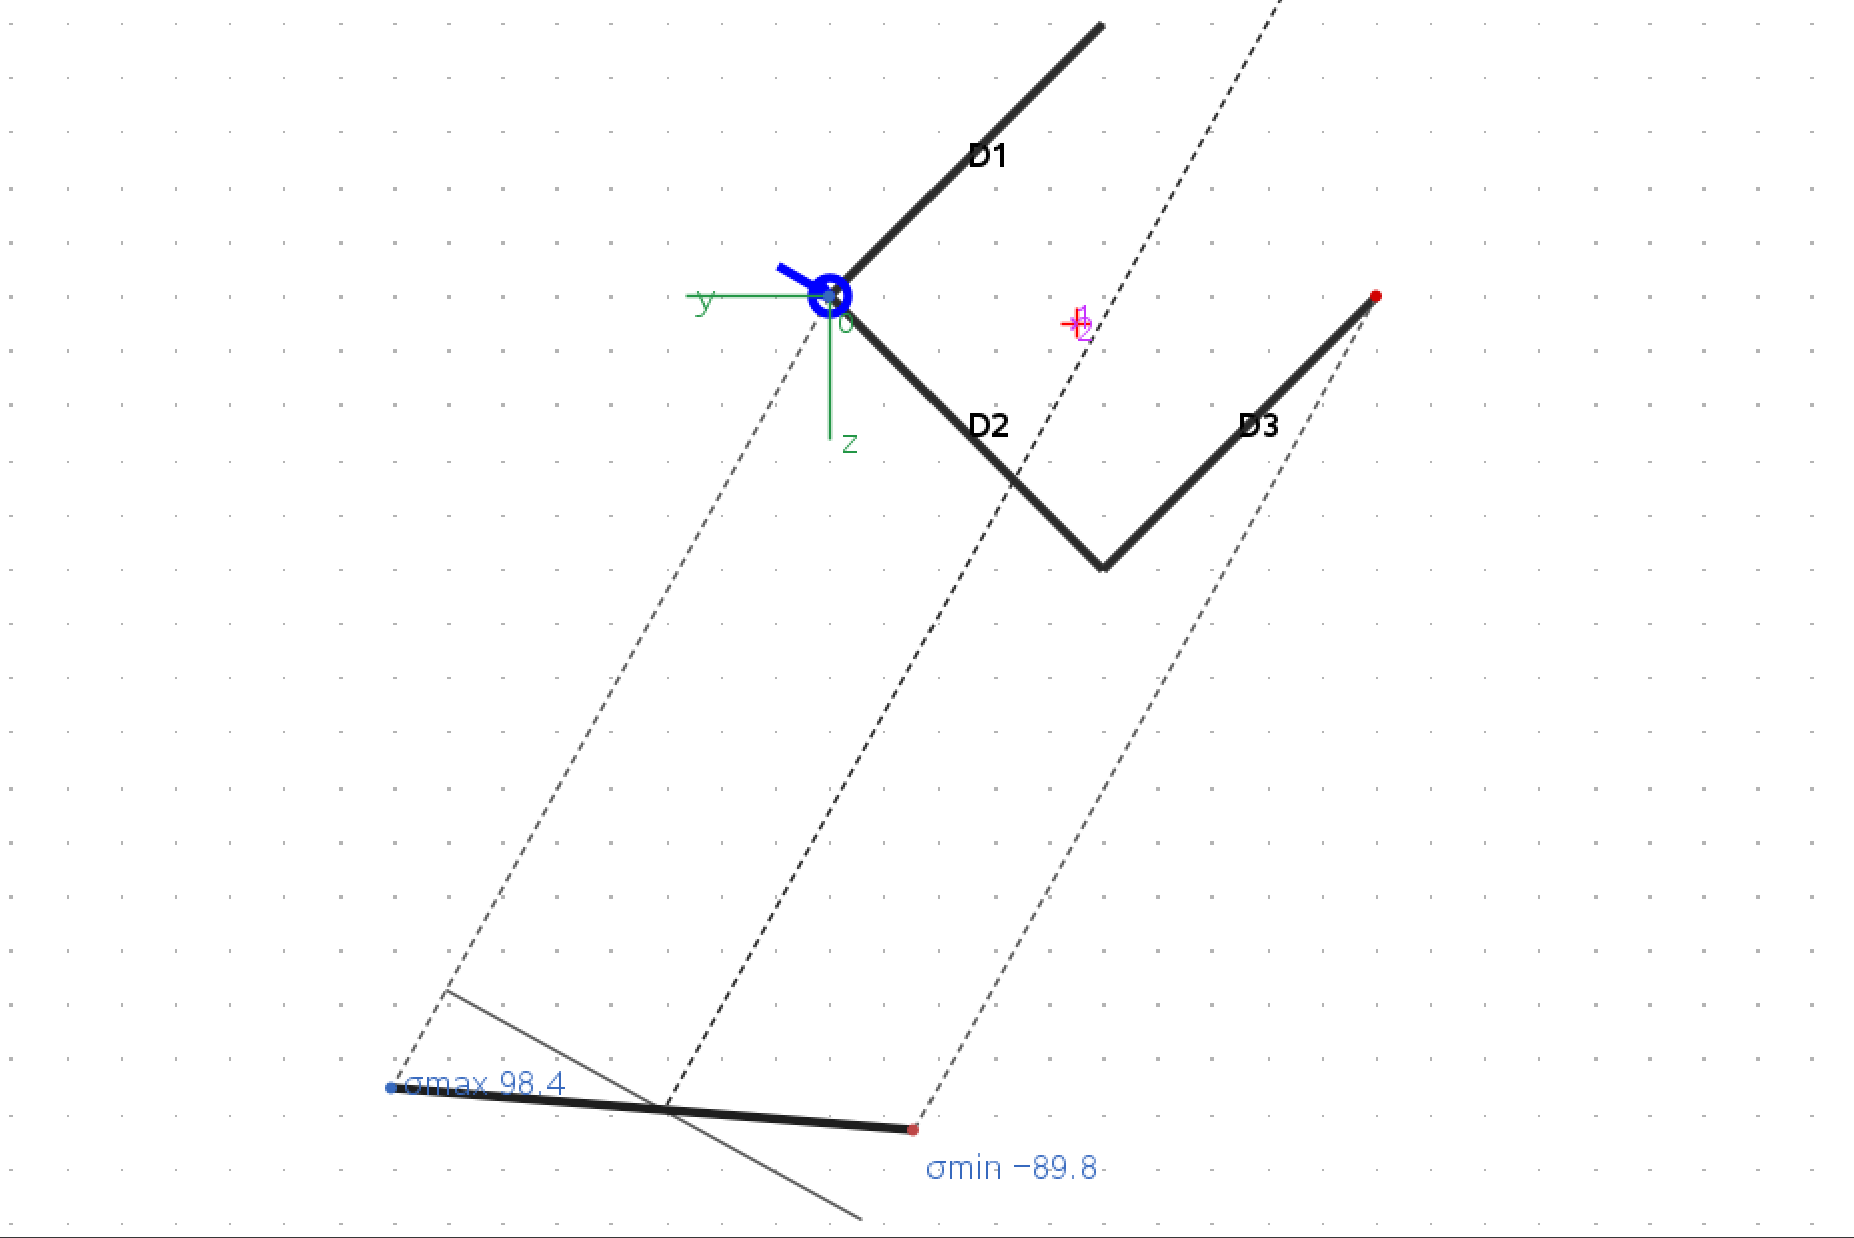
\includegraphics[width=\linewidth]{./fig/TM2/WiSe2526nr8_2.png}
        \caption{Spannungsverlauf}
    \end{subfigure}
    \hfill
    \begin{subfigure}[t]{0.48\textwidth}
        \centering
        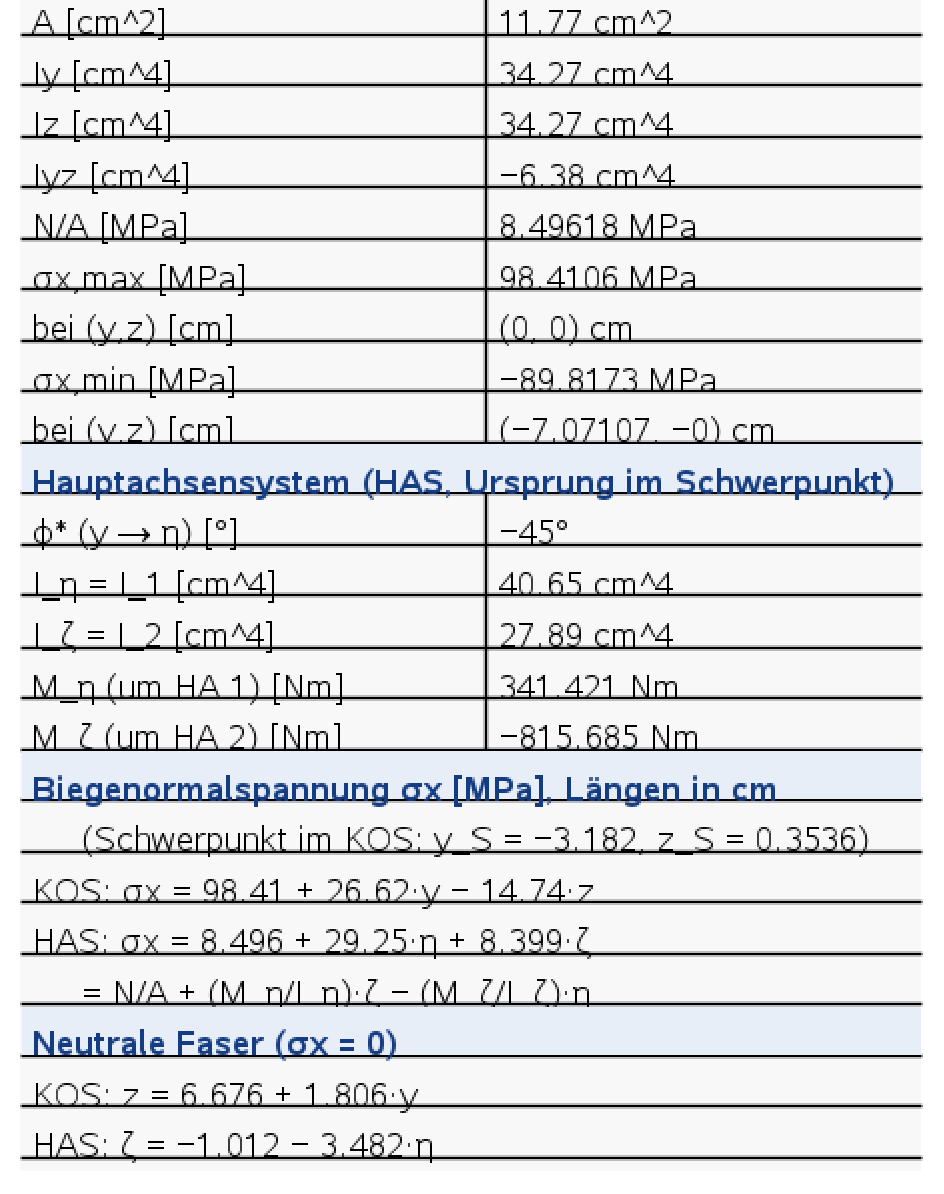
\includegraphics[width=\linewidth]{./fig/TM2/WiSe2526nr8_3.png}
        \caption{Tabellen übersicht}
    \end{subfigure}
    \caption{Lösung von TM2 WiSe~25/26, Nr.~8}
    \label{fig:TM2WiSe2526Nr8_2}
\end{figure}

Ich will anmereken, dass des öfteren bei Aufgaben Querschnittswerte gegeben sind, die nicht zur Bemaßung in der Zeichnung passen,
ob das absichtlich so ist konnte mir leider keiner sagen. Es ist also immer sinnvoll das einmal gegen zu prüfen und die Werte evtl. zu überschreiben.
Was die ISD-Musterlösung bei dieser Aufgabe gerechnet hat, ist mir nicht ganz klar. Meines Verständnisses nach wurde hier mit einem
Schwerpunkt für die Momente aus Normalkraft gerechnet, der genau in der Mitte des U profiels liegt, sodass die Normalkraft um die $y$-Achse kein Moment erzeugt.

\subsection{Schiefe Biegung/Kernfäche (TM2 WiSe21/22 Nr.~8)}



\subsection{MSK (TM2 WiSe 21/22 Nr.~3)}

Zu dieser Aufgabe gibt es eigentlich nicht besonders viel zu sagen, man gibt die gegebenen Werte ein und das Programm
füllt in grün die restlichen Werte auf (Abb.~\ref{fig:TM2WiSe2122Nr3_1}).

\begin{figure}[htbp]
    \centering
    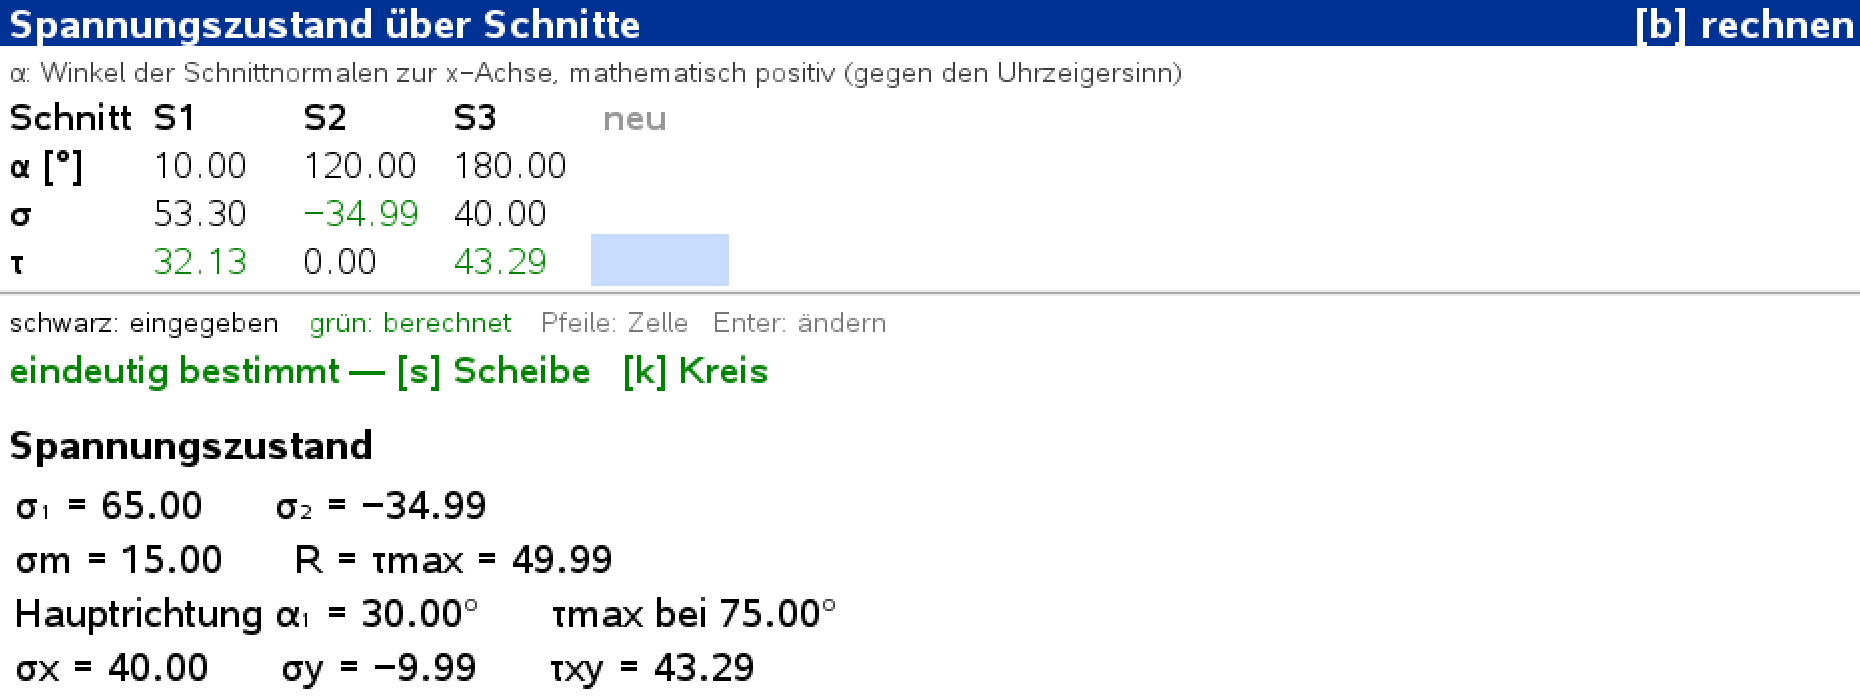
\includegraphics[width=0.7\linewidth]{./fig/TM2/WiSe2122nr3_1.png}
    \caption{TM2 WiSe~21/22, Nr.~3 im Programm}
    \label{fig:TM2WiSe2122Nr3_1}
\end{figure}

Danach bekommt man mit den Tasten \taste{s} und \taste{k} die beiden wichtigen Ansichten (Abb.~\ref{fig:TM2WiSe2122Nr3_2}).


\begin{figure}[htbp]
    \centering
    \begin{subfigure}[t]{0.48\textwidth}
        \centering
        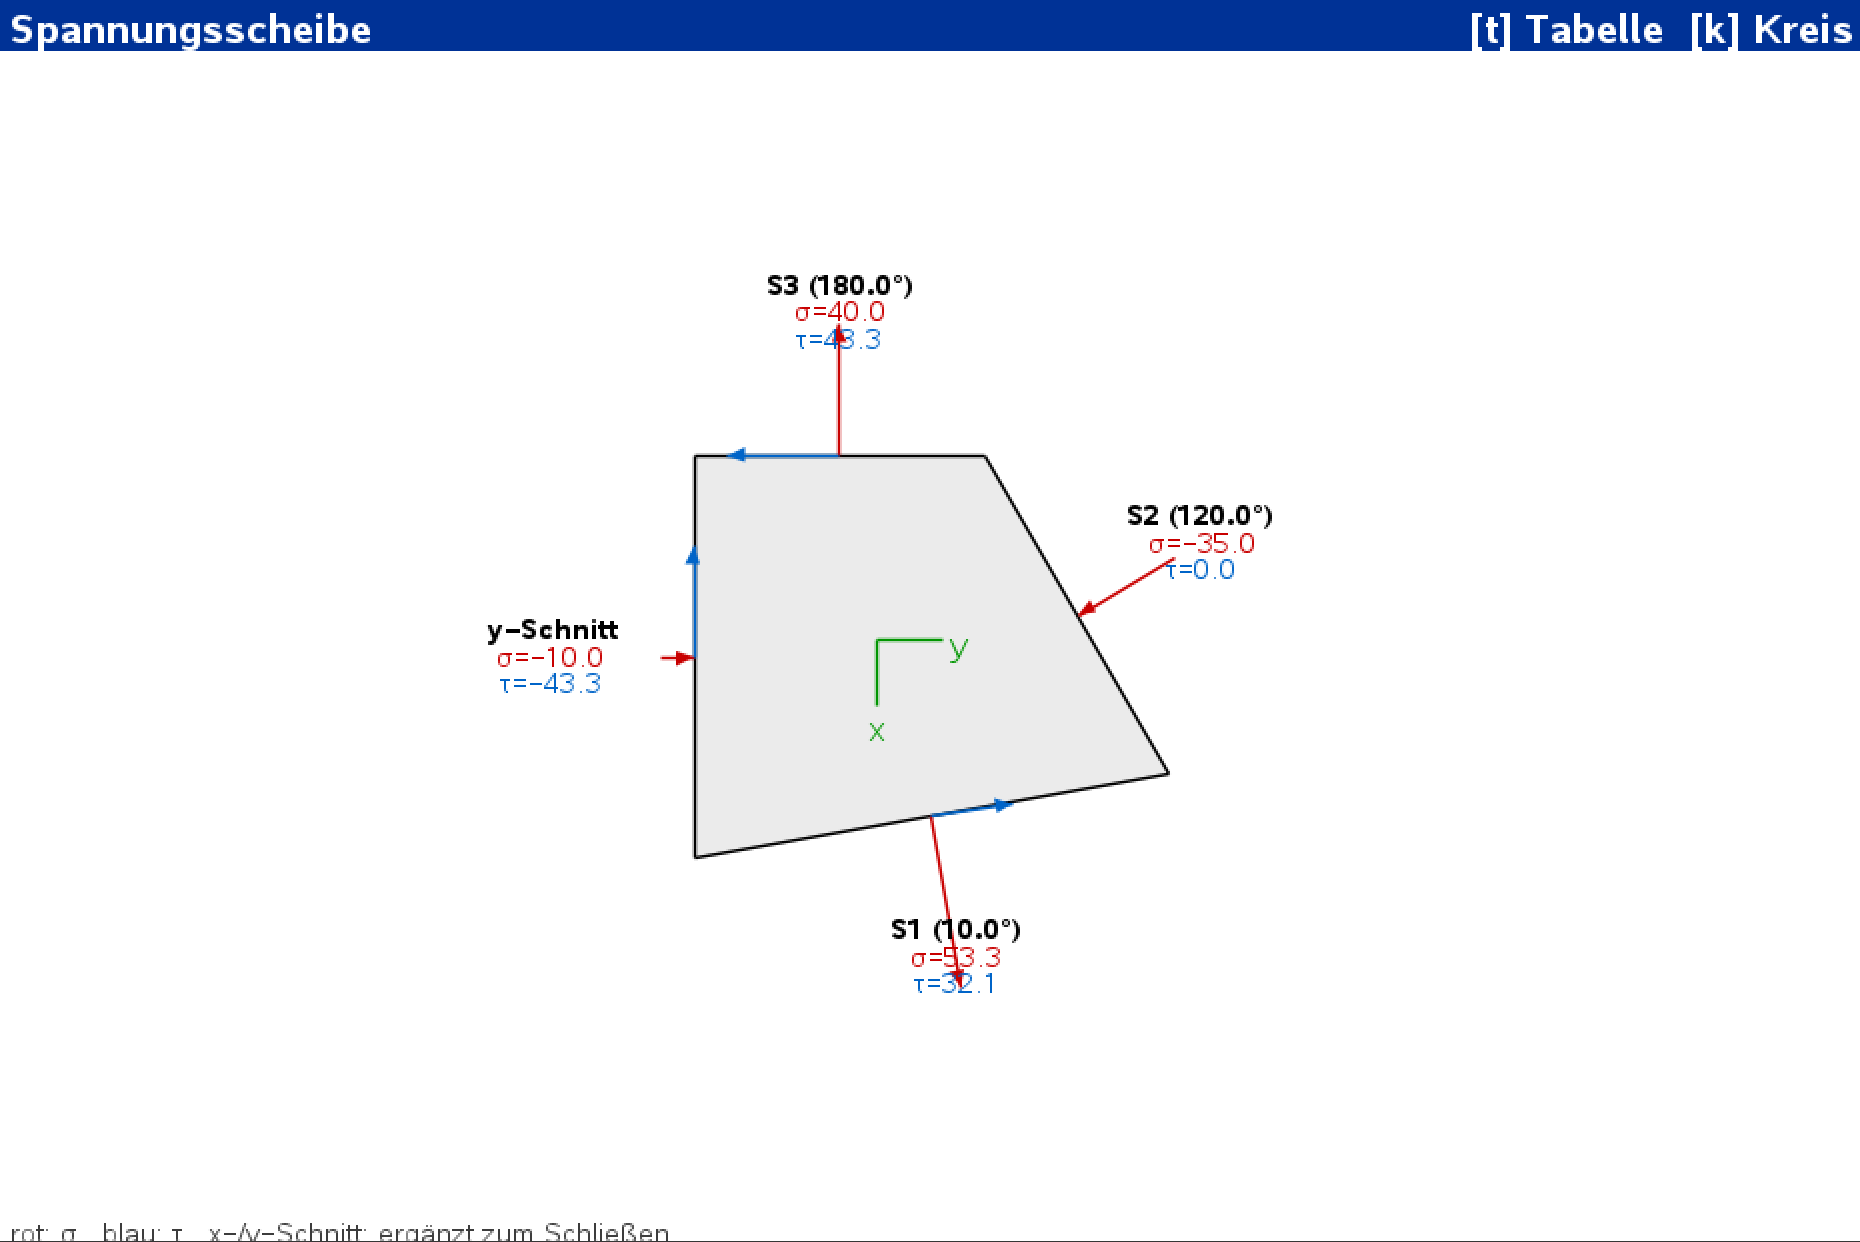
\includegraphics[width=\linewidth]{./fig/TM2/WiSe2122nr3_2.png}
        \caption{Spannungs-Scheibe}
    \end{subfigure}
    \hfill
    \begin{subfigure}[t]{0.48\textwidth}
        \centering
        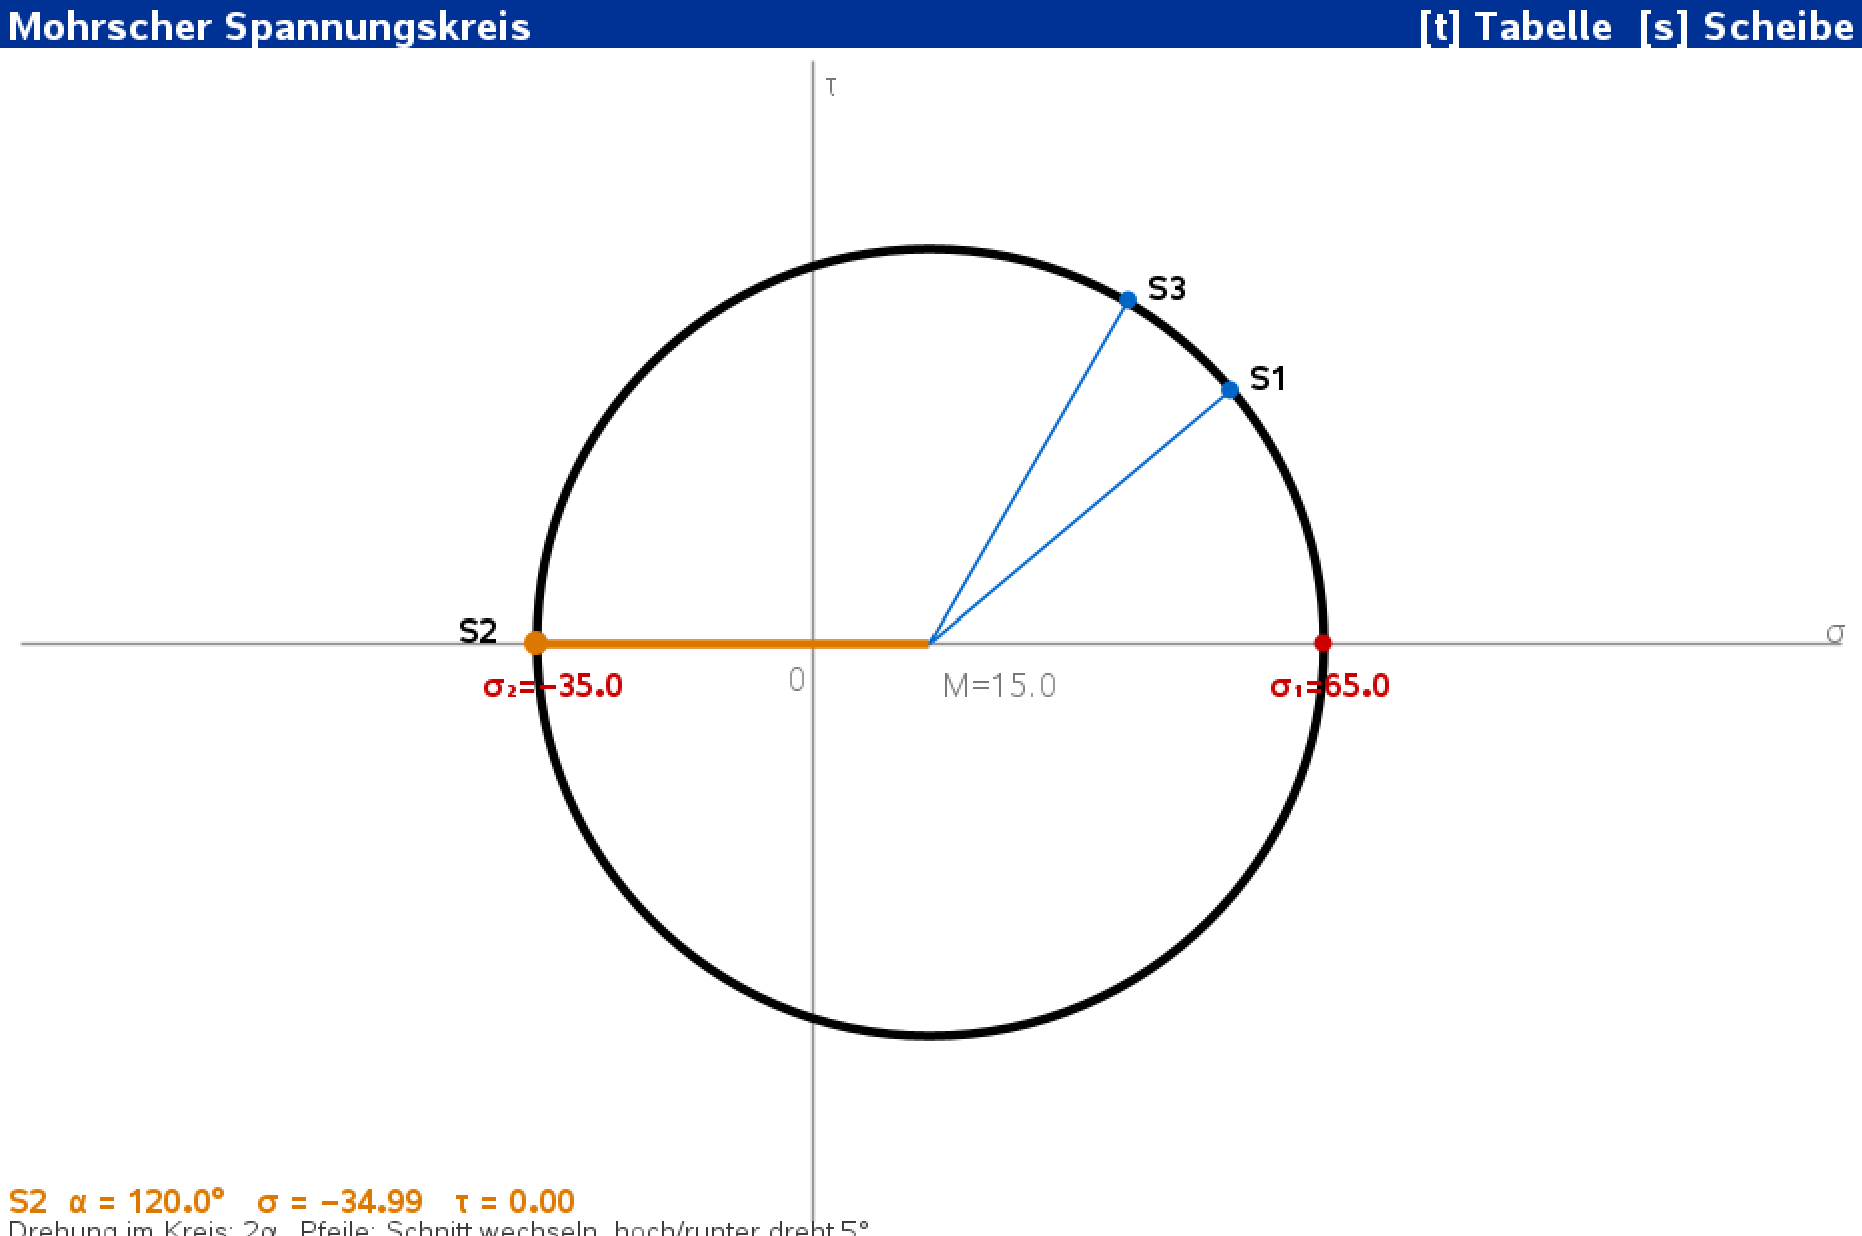
\includegraphics[width=\linewidth]{./fig/TM2/WiSe2122nr3_3.png}
        \caption{Spannungs-Kreis}
    \end{subfigure}
    \caption{Lösung von TM2 WiSe~21/22, Nr.~3}
    \label{fig:TM2WiSe2122Nr3_2}
\end{figure}

Falls bei einer Aufgabe nach dem Winkel eines Schnitts gefragt wird und das Programm zwei Winkel ausgibt, muss natürlich
geprüft werden, welcher Winkel eher zur Skizze passt.

\subsection{Schubspannung und SMP (TM2 SoSe 24 Nr.~8)}

\subsection{Verwölbung (TM2 SoSe 20 Nr.~9)} eingebunden.
% Hier keine \usepackage-Zeilen: Pakete stehen in der Praeambel von Anleitung.tex.
% Abbildungen mit [htbp]: LaTeX setzt sie dann dorthin, wo Platz ist. Im Text deshalb immer
% mit Abb.~\ref{...} auf sie verweisen, nicht mit "unten" oder "folgendermaßen".


\part{Beispiele}

In diesem Teil will ich anhand typischer Klausuraufgaben etwas genauer beschreiben, wie man das
Programm am besten verwendet, zumindest so, wie ich es für sinnvoll halte.

Die Screenshots habe ich in der PC-Ansicht gemacht, weil dort viele Dinge besser erkennbar sind.
Auf dem Taschenrechner selbst sollte mit Zoom aber auch alles erkennbar sein.

\section{TM1}
\subsection{WiSe~21/22}
\subsubsection{Geschlossenes System (Nr.~2)}
Bei dieser Aufgabe gibt es ein paar Besonderheiten bei der Eingabe, deshalb stelle ich sie hier vor.
Im Programm sieht das Tragwerk aus wie in Abb.~\ref{fig:WiSe2122nr2_1}.

\begin{figure}[htbp]
    \centering
    \begin{subfigure}[t]{0.48\textwidth}
        \centering
        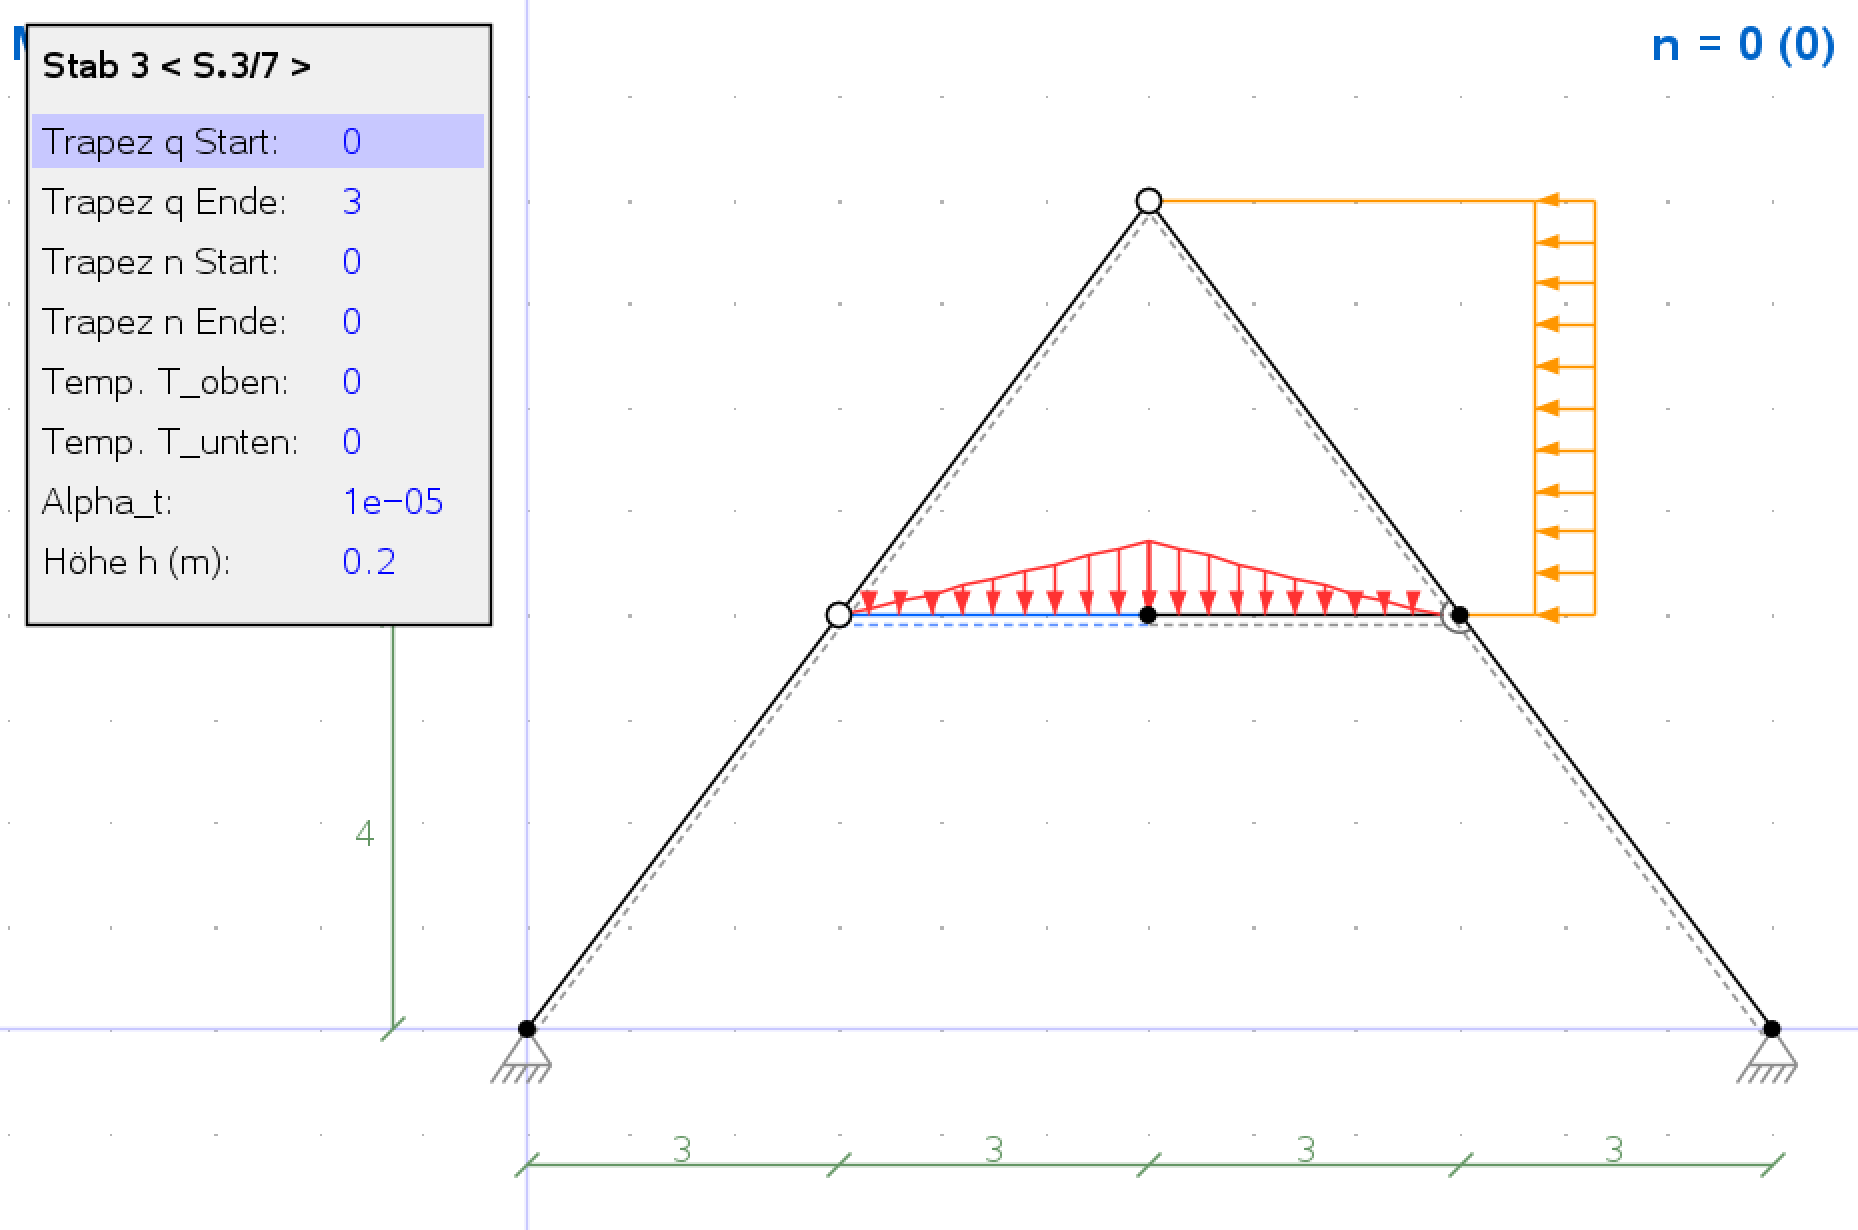
\includegraphics[width=\linewidth]{./fig/TM1/WiSe2122nr2_1.png}
        \caption{Trapezlast auf der linken Hälfte des Mittelstabs}
    \end{subfigure}
    \hfill
    \begin{subfigure}[t]{0.48\textwidth}
        \centering
        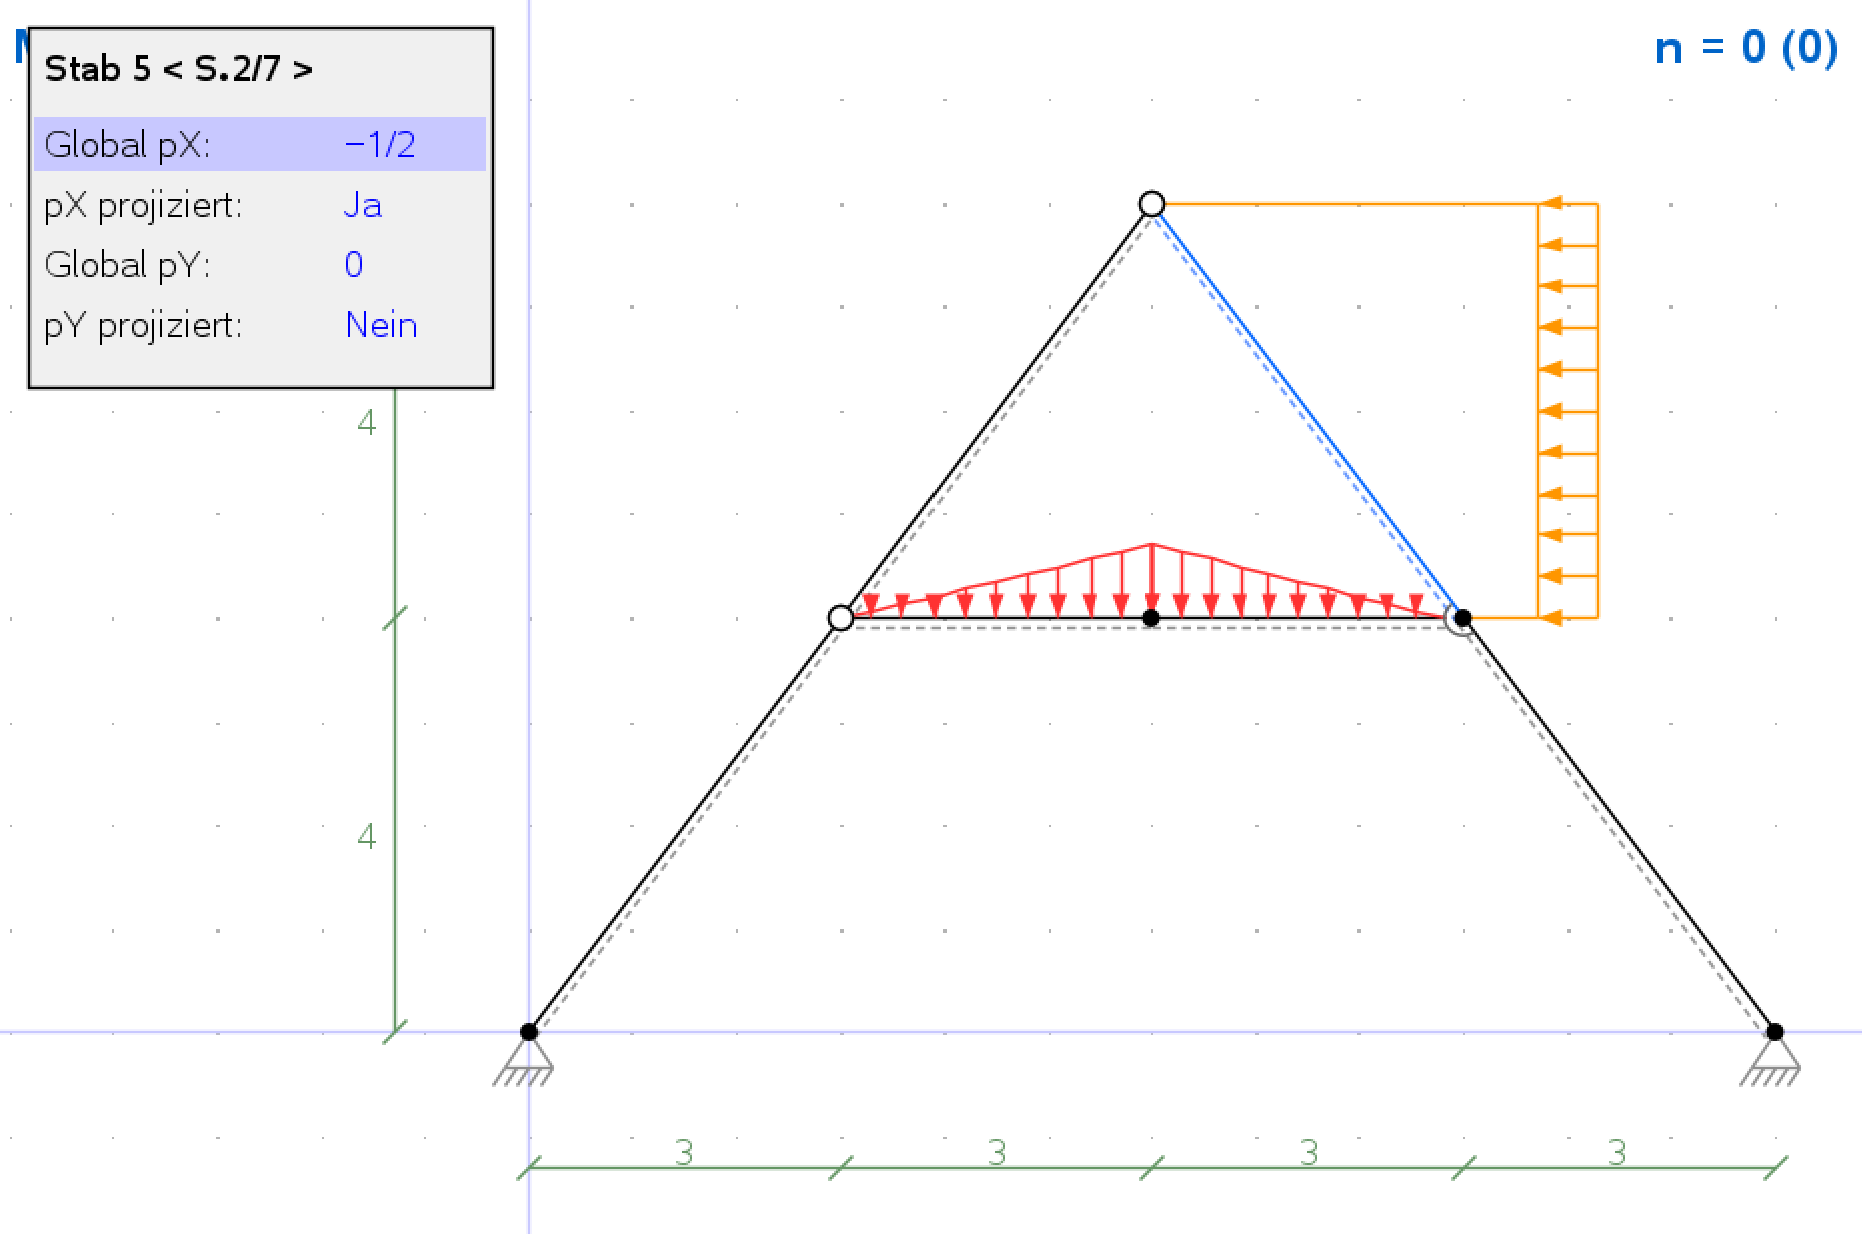
\includegraphics[width=\linewidth]{./fig/TM1/WiSe2122nr2_2.png}
        \caption{globale Streckenlast am oberen rechten Stab}
    \end{subfigure}
    \caption{WiSe~21/22, Nr.~2 im Programm}
    \label{fig:WiSe2122nr2_1}
\end{figure}

Den Stab in der Mitte müsst ihr im Programm teilen. Die Last auf ihm ist dreieckförmig mit der
Spitze in der Mitte, eine Trapezlast geht aber immer über einen ganzen Stab. Jede Hälfte bekommt
deshalb ihre eigene Trapezlast, die linke von $0$ auf $3$, die rechte von $3$ auf $0$
(Abb.~\ref{fig:WiSe2122nr2_1}a). Der neue Knoten in der Mitte bleibt biegesteif.

Die Streckenlast am schrägen Stab gebt ihr am einfachsten als globale Last ein
(Abb.~\ref{fig:WiSe2122nr2_1}b). In der Aufgabe ist sie auf die senkrechte Projektion des Stabes
bezogen, deshalb muss \emph{pX projiziert} auf \emph{Ja} stehen. Negativ ist sie, weil sie global
gesehen entgegen der $x$-Achse wirkt, also nach links.

Nach dem Berechnen könnt ihr das LGS, das zur Explosionsansicht (Abb.~\ref{fig:WiSe2122nr2_2})
gehört, über die zweite Seite des Obermenüs (\emph{LGS-Matrix}) in den Taschenrechner exportieren
(Abb.~\ref{fig:WiSe2122nr2_3}). Die Gleichungen stehen dann lesbar in \code{lgs}, die Lösung
bekommt ihr zum Beispiel mit \code{ggw\_x = ggw\_a$^{-1}$*ggw\_b}
(Abschnitt~\ref{sec:lgs-matrix}).

\begin{figure}[htbp]
    \centering
    \begin{subfigure}[t]{0.48\textwidth}
        \centering
        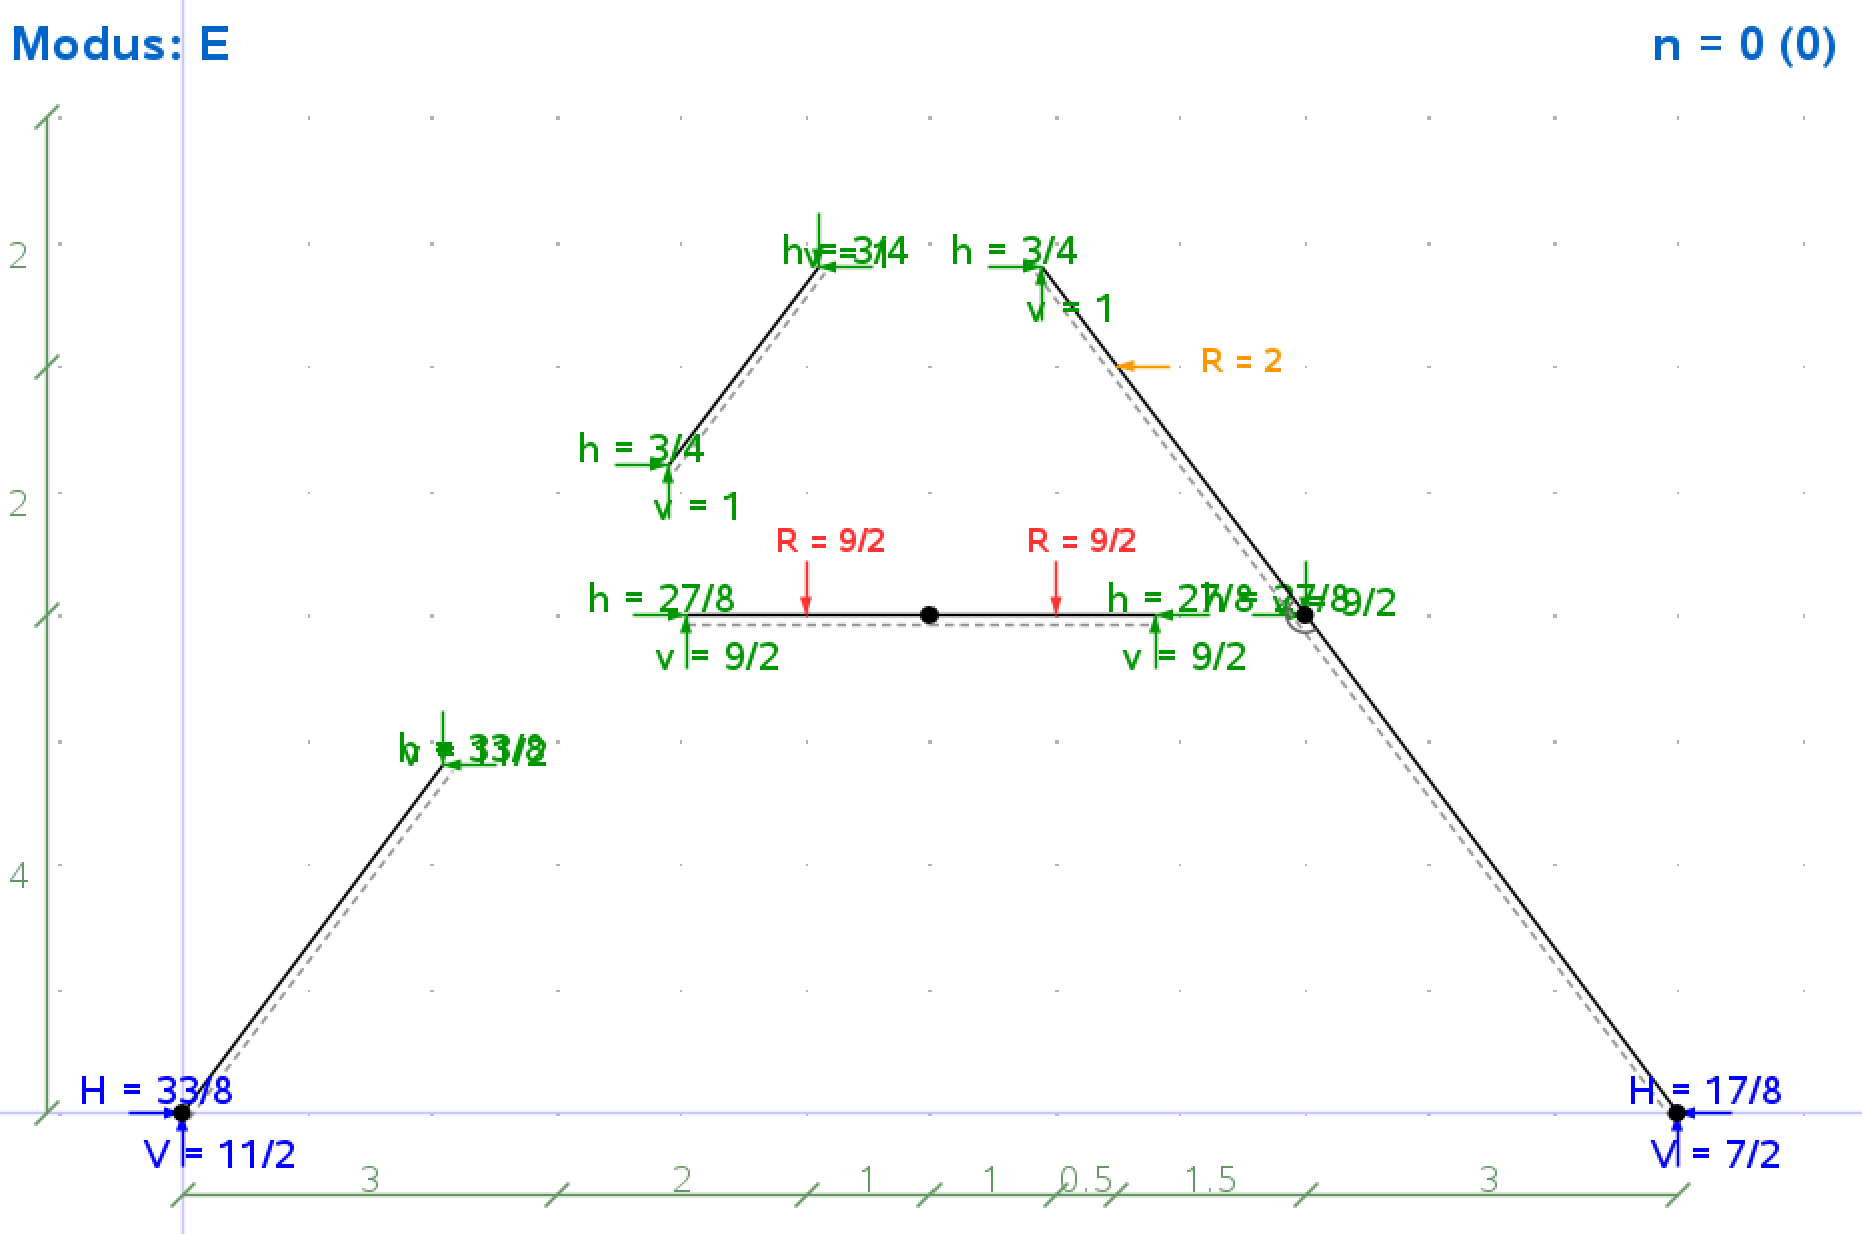
\includegraphics[width=\linewidth]{./fig/TM1/WiSe2122nr2_5.png}
        \caption{Seite~1: Ergebnisse in ihrer wirklichen Richtung}
    \end{subfigure}
    \hfill
    \begin{subfigure}[t]{0.48\textwidth}
        \centering
        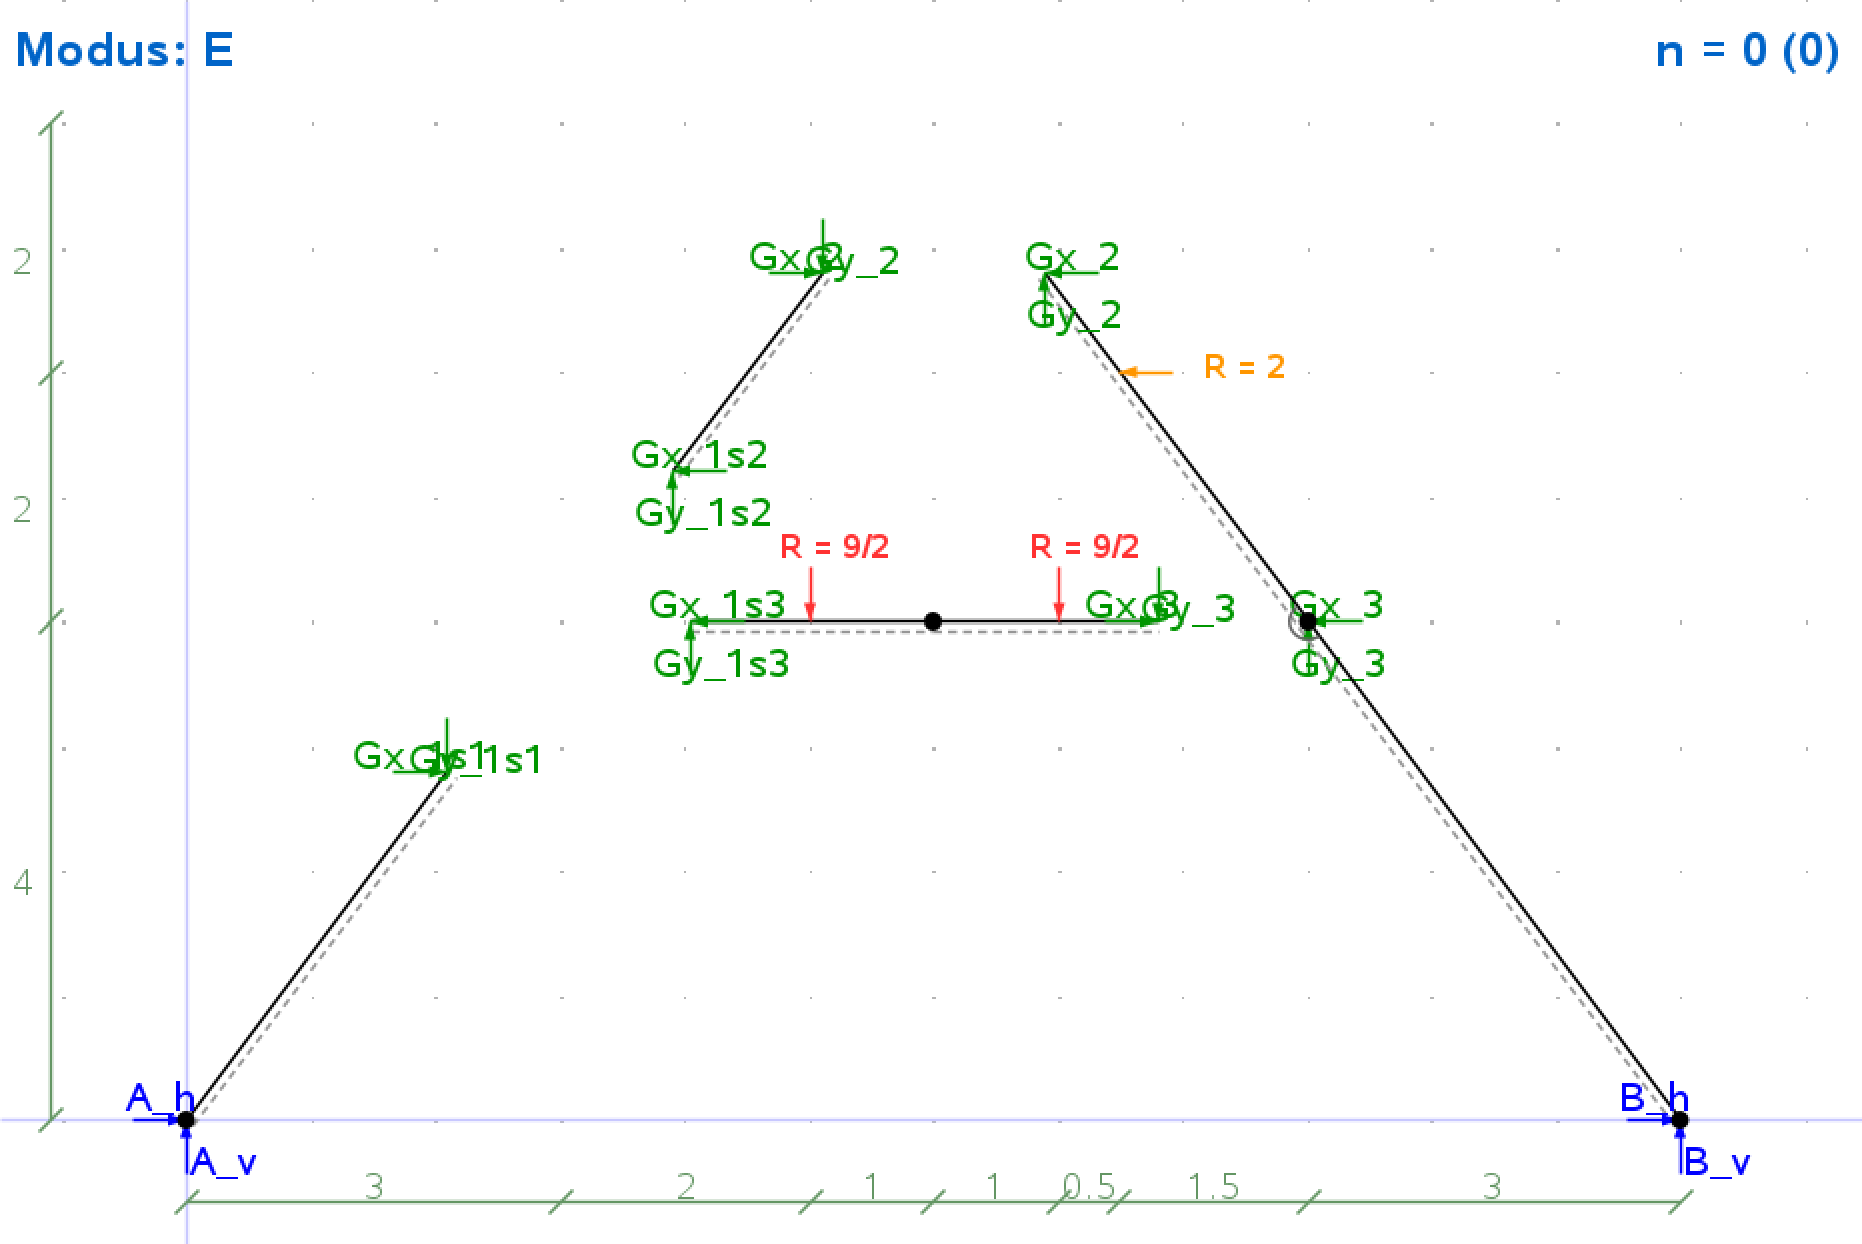
\includegraphics[width=\linewidth]{./fig/TM1/WiSe2122nr2_6.png}
        \caption{Seite~2: Unbekannte in positiver Richtung}
    \end{subfigure}
    \caption{WiSe~21/22, Nr.~2: Explosionsansicht (E-Modus)}
    \label{fig:WiSe2122nr2_2}
\end{figure}

\begin{figure}[htbp]
    \centering
    \begin{subfigure}[t]{0.48\textwidth}
        \centering
        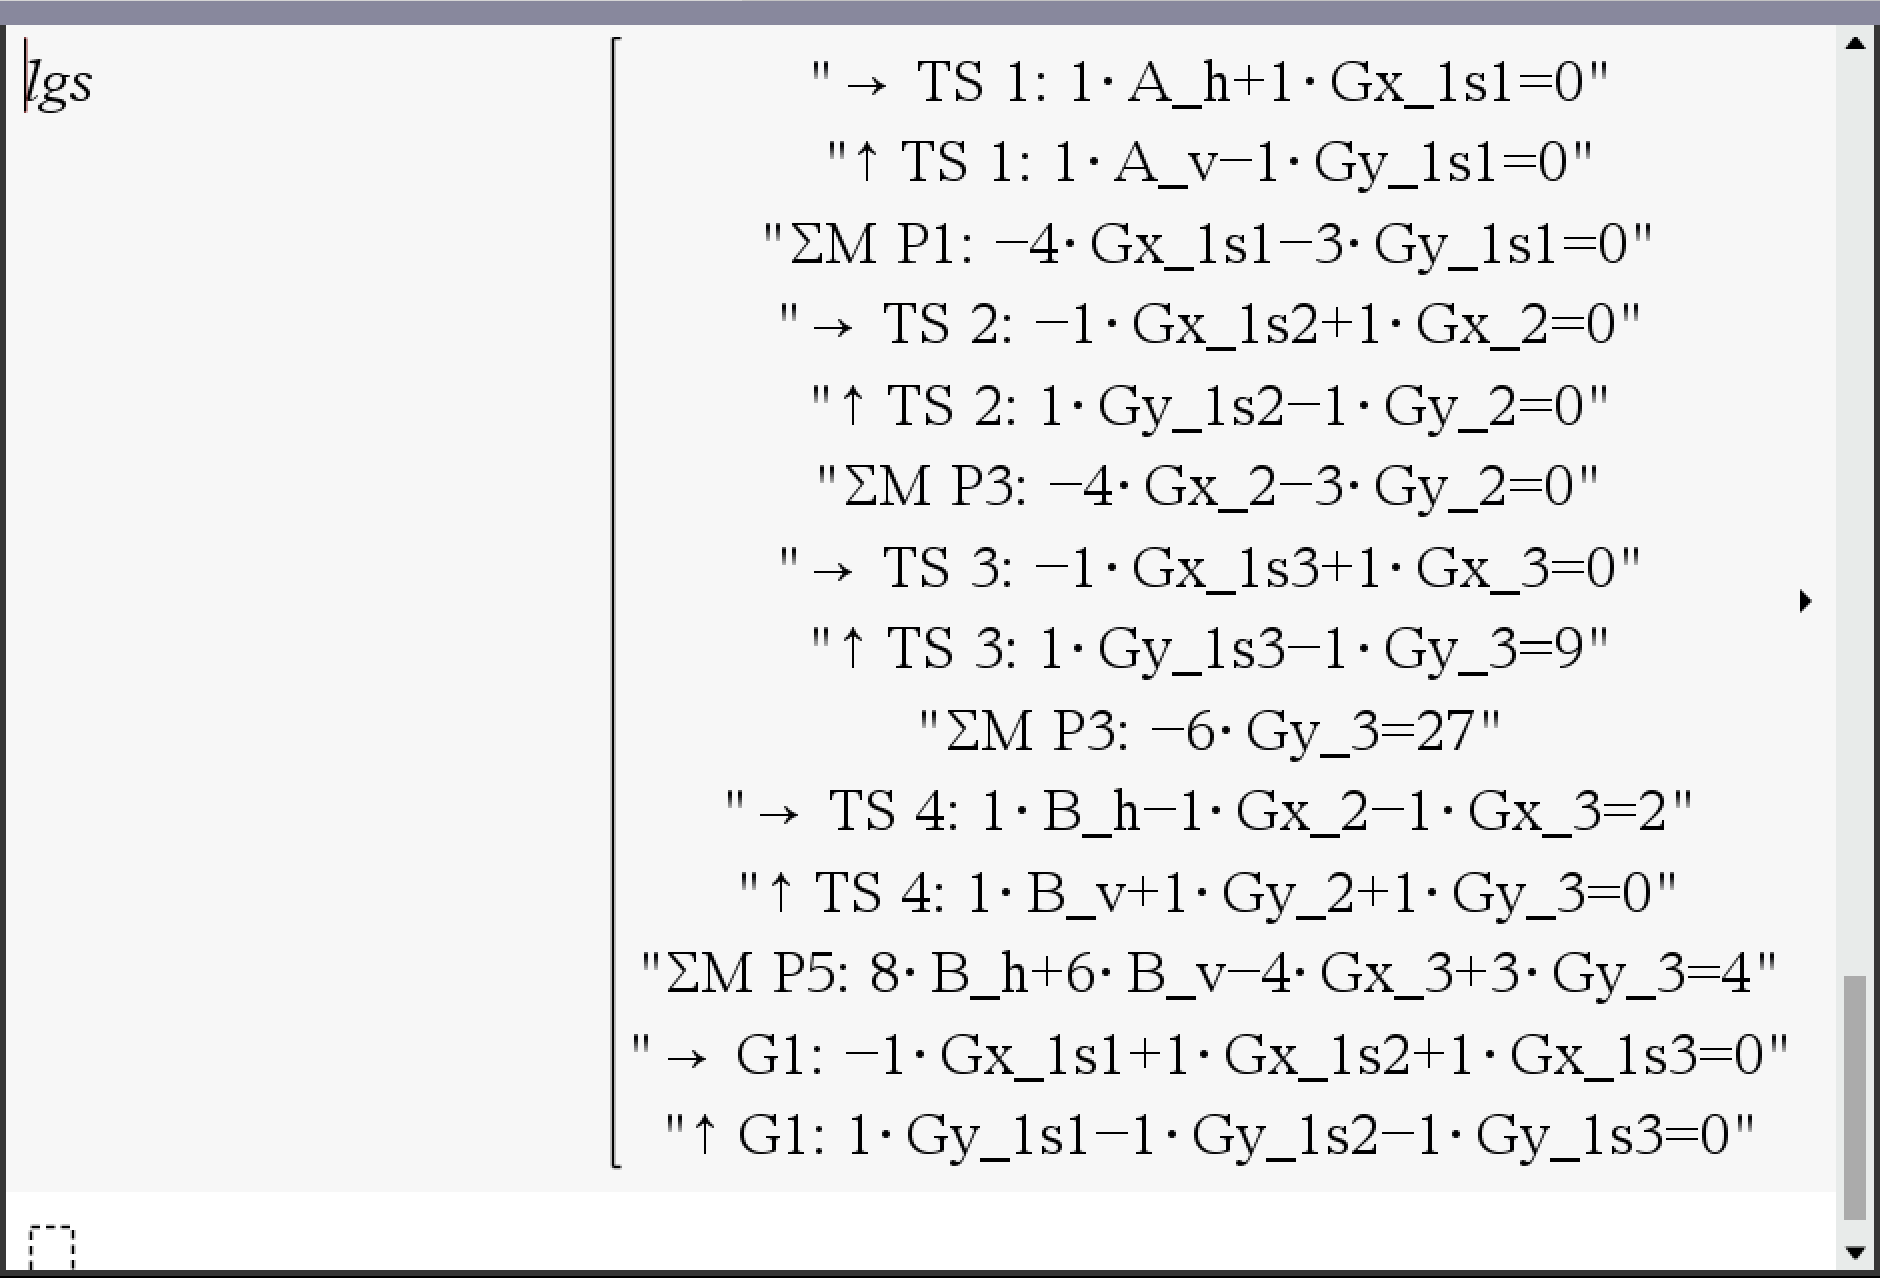
\includegraphics[width=\linewidth]{./fig/TM1/WiSe2122nr2_3.png}
        \caption{exportierte Gleichungen \code{lgs}}
    \end{subfigure}
    \hfill
    \begin{subfigure}[t]{0.48\textwidth}
        \centering
        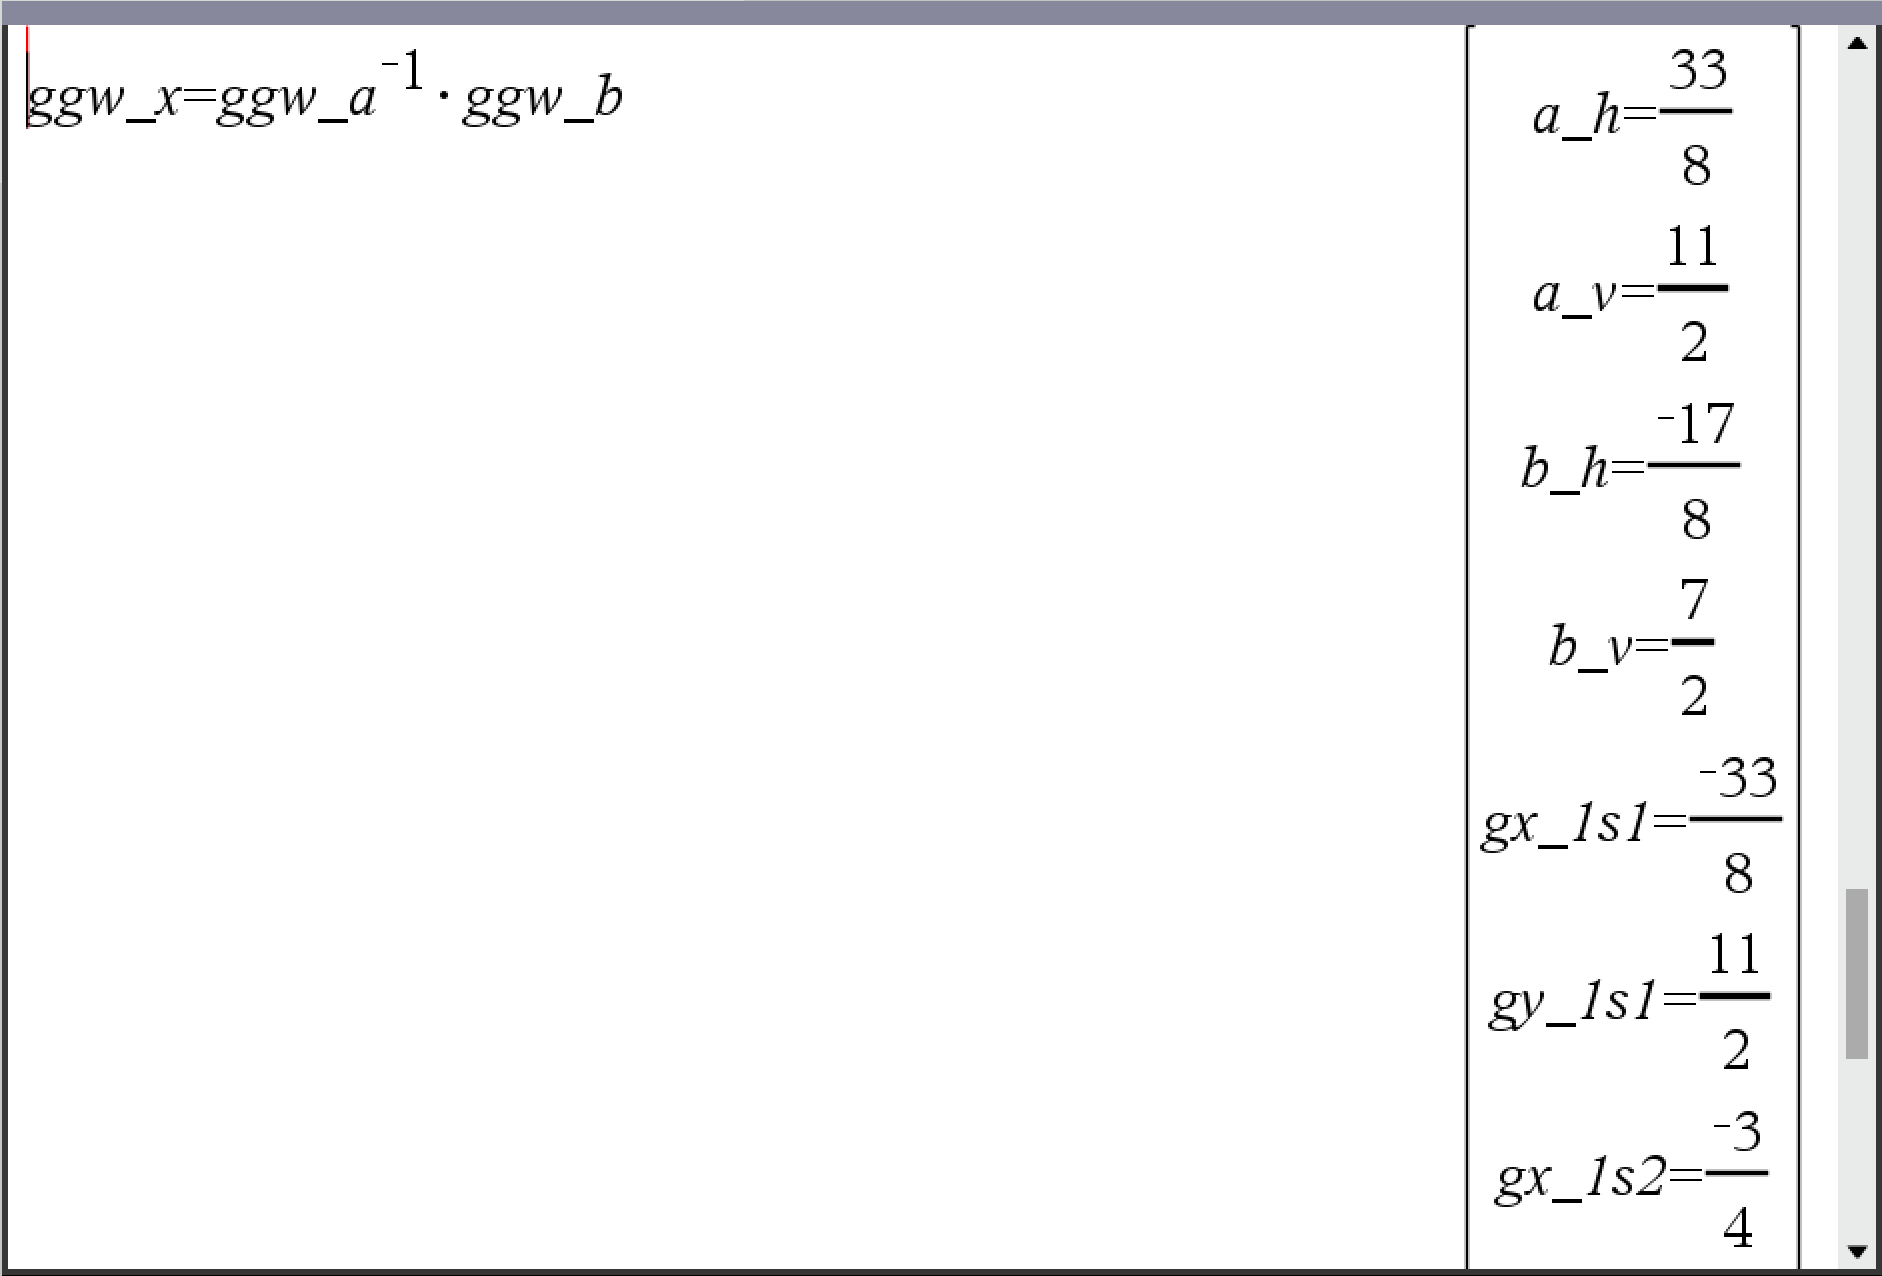
\includegraphics[width=\linewidth]{./fig/TM1/WiSe2122mr2_4.png}
        \caption{Lösung mit \code{ggw\_x}}
    \end{subfigure}
    \caption{WiSe~21/22, Nr.~2: exportiertes LGS}
    \label{fig:WiSe2122nr2_3}
\end{figure}

Die Explosionsansicht kann manchmal etwas unübersichtlich sein. Wenn ihr nah genug heranzoomt,
sollte aber trotzdem alles erkennbar sein. Die Ergebnisse müsst ihr natürlich nicht in dieser
Vektorform aufschreiben, nur ihr Inhalt zählt.

An dieser Stelle will ich anmerken, dass meist nur bei Systemen mit einem geschlossenen Ring wie
diesem nach allen Gelenk- und Auflagerkräften gefragt wird. Bei offenen Systemen ohne Ring wird oft
nur nach den Auflagerkräften gefragt. Das exportierte LGS liefert dann zwar auch die richtige Lösung, ist aber
meist mehr, als ihr braucht. Den Punkt, um den das Programm die Momentensumme eines Teilsystems
bildet, seht ihr, wenn ihr in der Explosionsansicht mit der Maus über das Teilsystem fahrt
(\emph{Hover}).

Die Zustandslinien, also die Verläufe der Schnittgrößen, zeichnet euch das Programm mit den Tasten
\taste{n}, \taste{q} und \taste{m}, die könnt ihr einfach abzeichnen. Falls ihr Randwerte schlecht
erkennt, fahrt mit der Maus über den jeweiligen Stab, dann zeigt das Programm nur noch diesen Stab
mit seinen Randwerten an.

\subsubsection{Qualitavtive Verläufe im symbolischen Modus (Nr.~4)}

Um meinen den oben genannten Punkt zum symbolischen Modus zu verdeutlichen will ich hier kurz auf Teilaufgabe b) eingehen.
Das System und der Querkraftverlauf sind in Abbildung~\ref{fig:TM1WiSe2122Nr4} dargestellt.

\begin{figure}[htbp]
    \centering
    \begin{subfigure}[t]{0.48\textwidth}
        \centering
        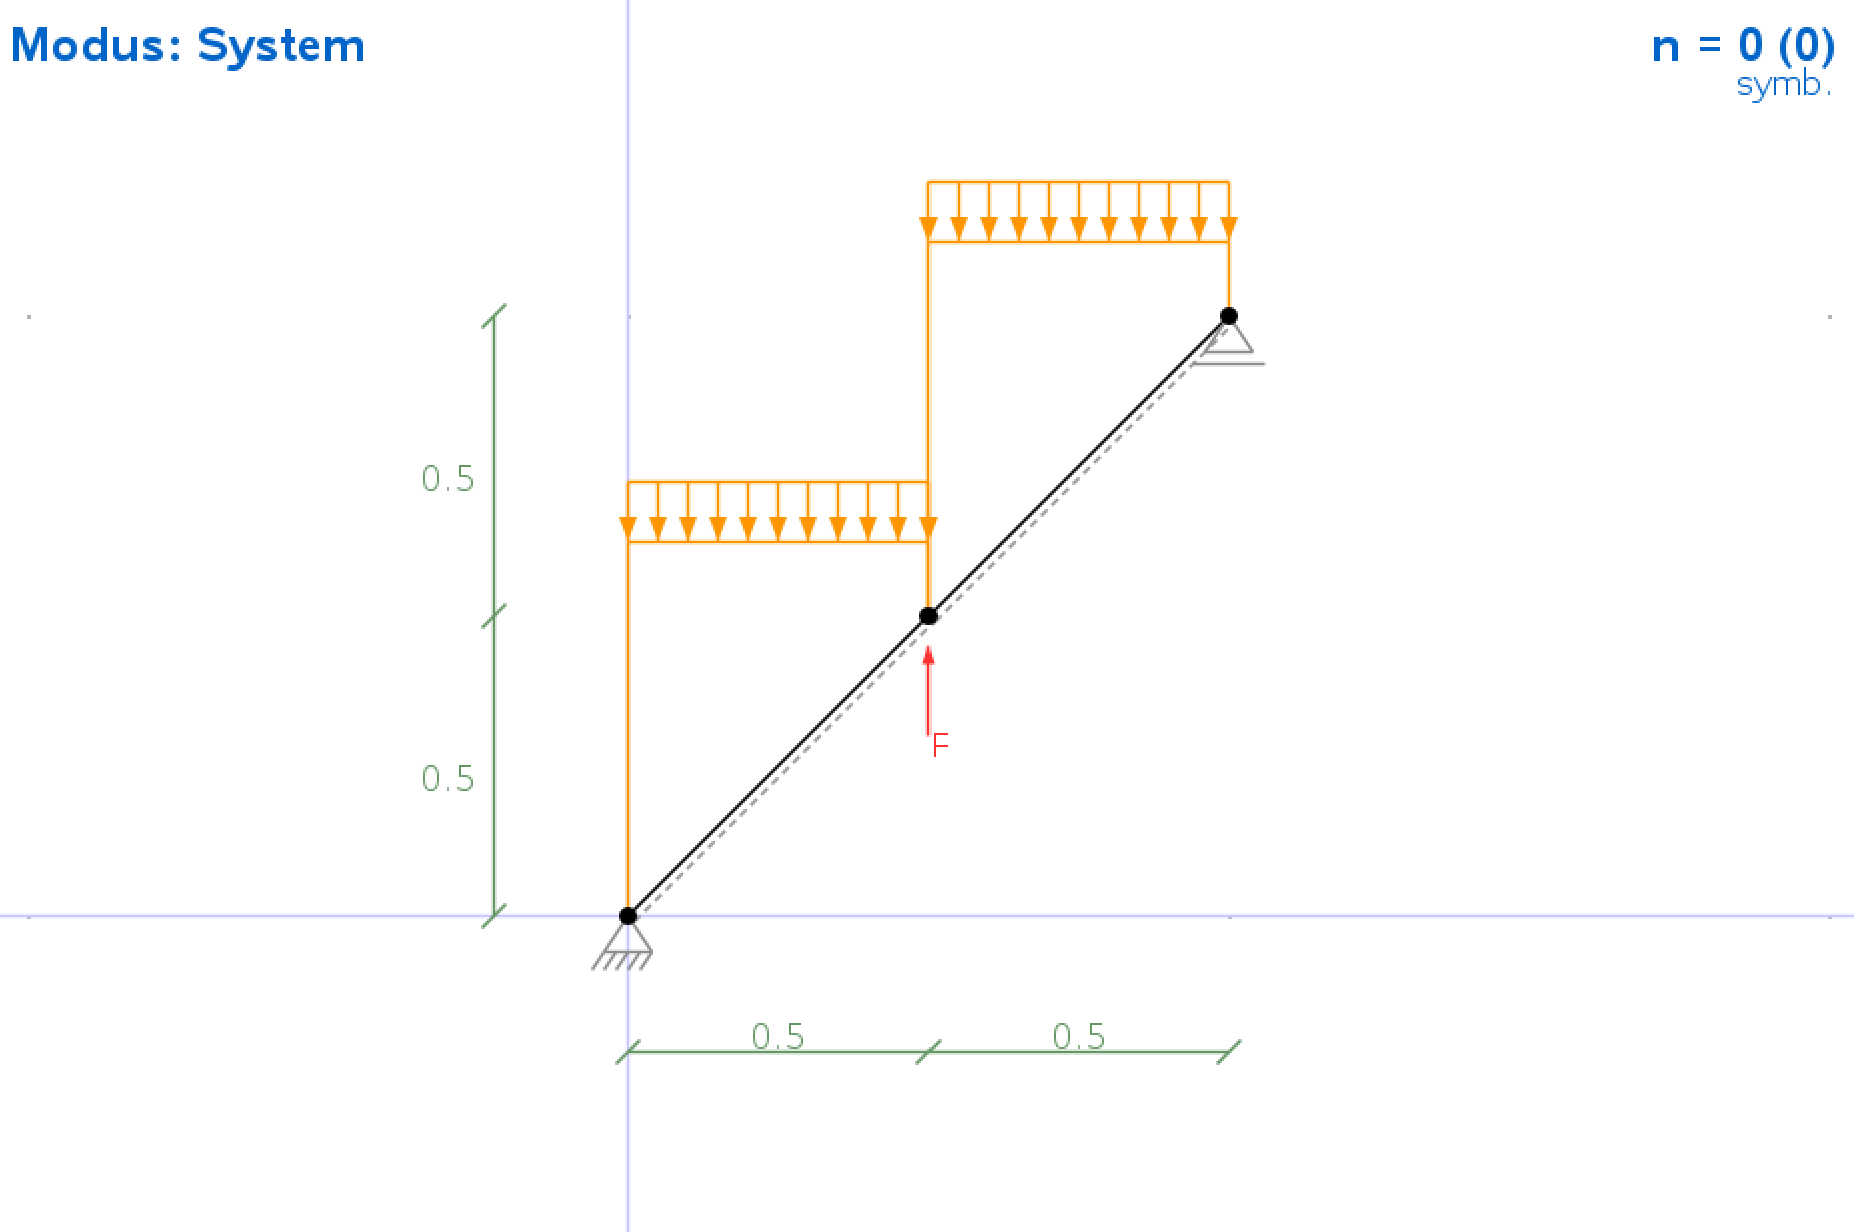
\includegraphics[width=\linewidth]{./fig/TM1/WiSe2122nr4_1.png}
        \caption{System}
    \end{subfigure}
    \hfill
    \begin{subfigure}[t]{0.48\textwidth}
        \centering
        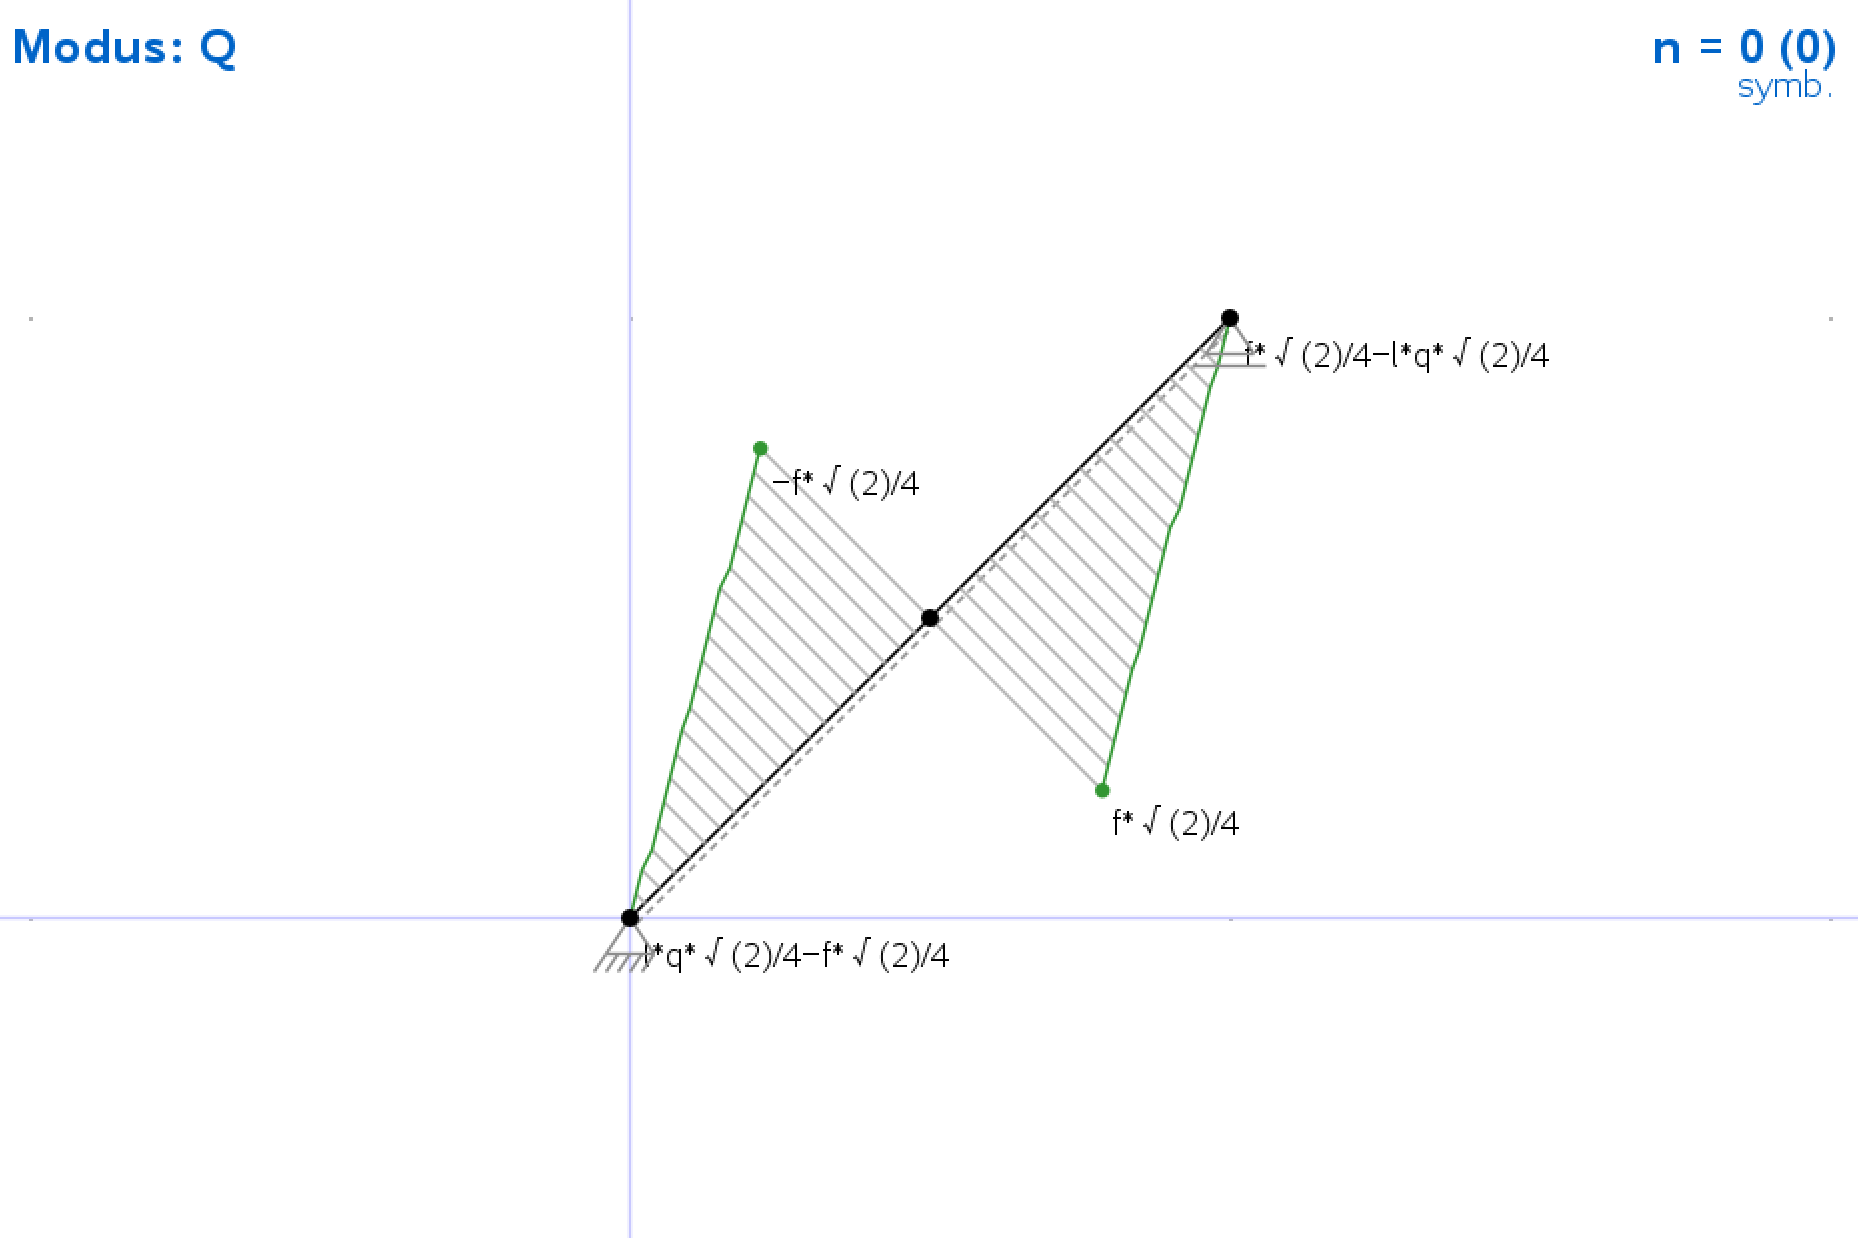
\includegraphics[width=\linewidth]{./fig/TM1/WiSe2122nr4_2.png}
        \caption{Querkraftverlauf}
    \end{subfigure}
    \caption{WiSe~21/22, Nr.~4}
    \label{fig:TM1WiSe2122Nr4}
\end{figure}

Im Querkraft verlauf sieht es so aus, als ob diese an den Auflagern null wird. Wenn man sich die Beschriftung der Randwerte 
anschaut wird jedoch klar, dass ist nur der Fall, wenn $q\cdot l=F$ bzw. $q\cdot a=F$ gilt. Das ist eben genau die Annhame des Programms,
um überhaupt irgendeinen Verlauf zeichnen zu können.
Die Aufgabe gibt aber unten vor: $F>q\cdot a$. Damit wird die Qerkraft am linekn Ende negativ und am rechten Ende positiv.
Die Verläufe von symbolische Berechnungen solltet ihr also \textbf{nie} einfach blind abzeichnen.

\subsection{PvV (Nr.~3)}

Zum PvV gibt es eigentlich nicht viel zu sagen. System zeichnen, \taste{v} drücken, Bindung wählen, abzeichnen,
dann exportieren und aufschreiben. 


\begin{figure}[htbp]
    \centering
    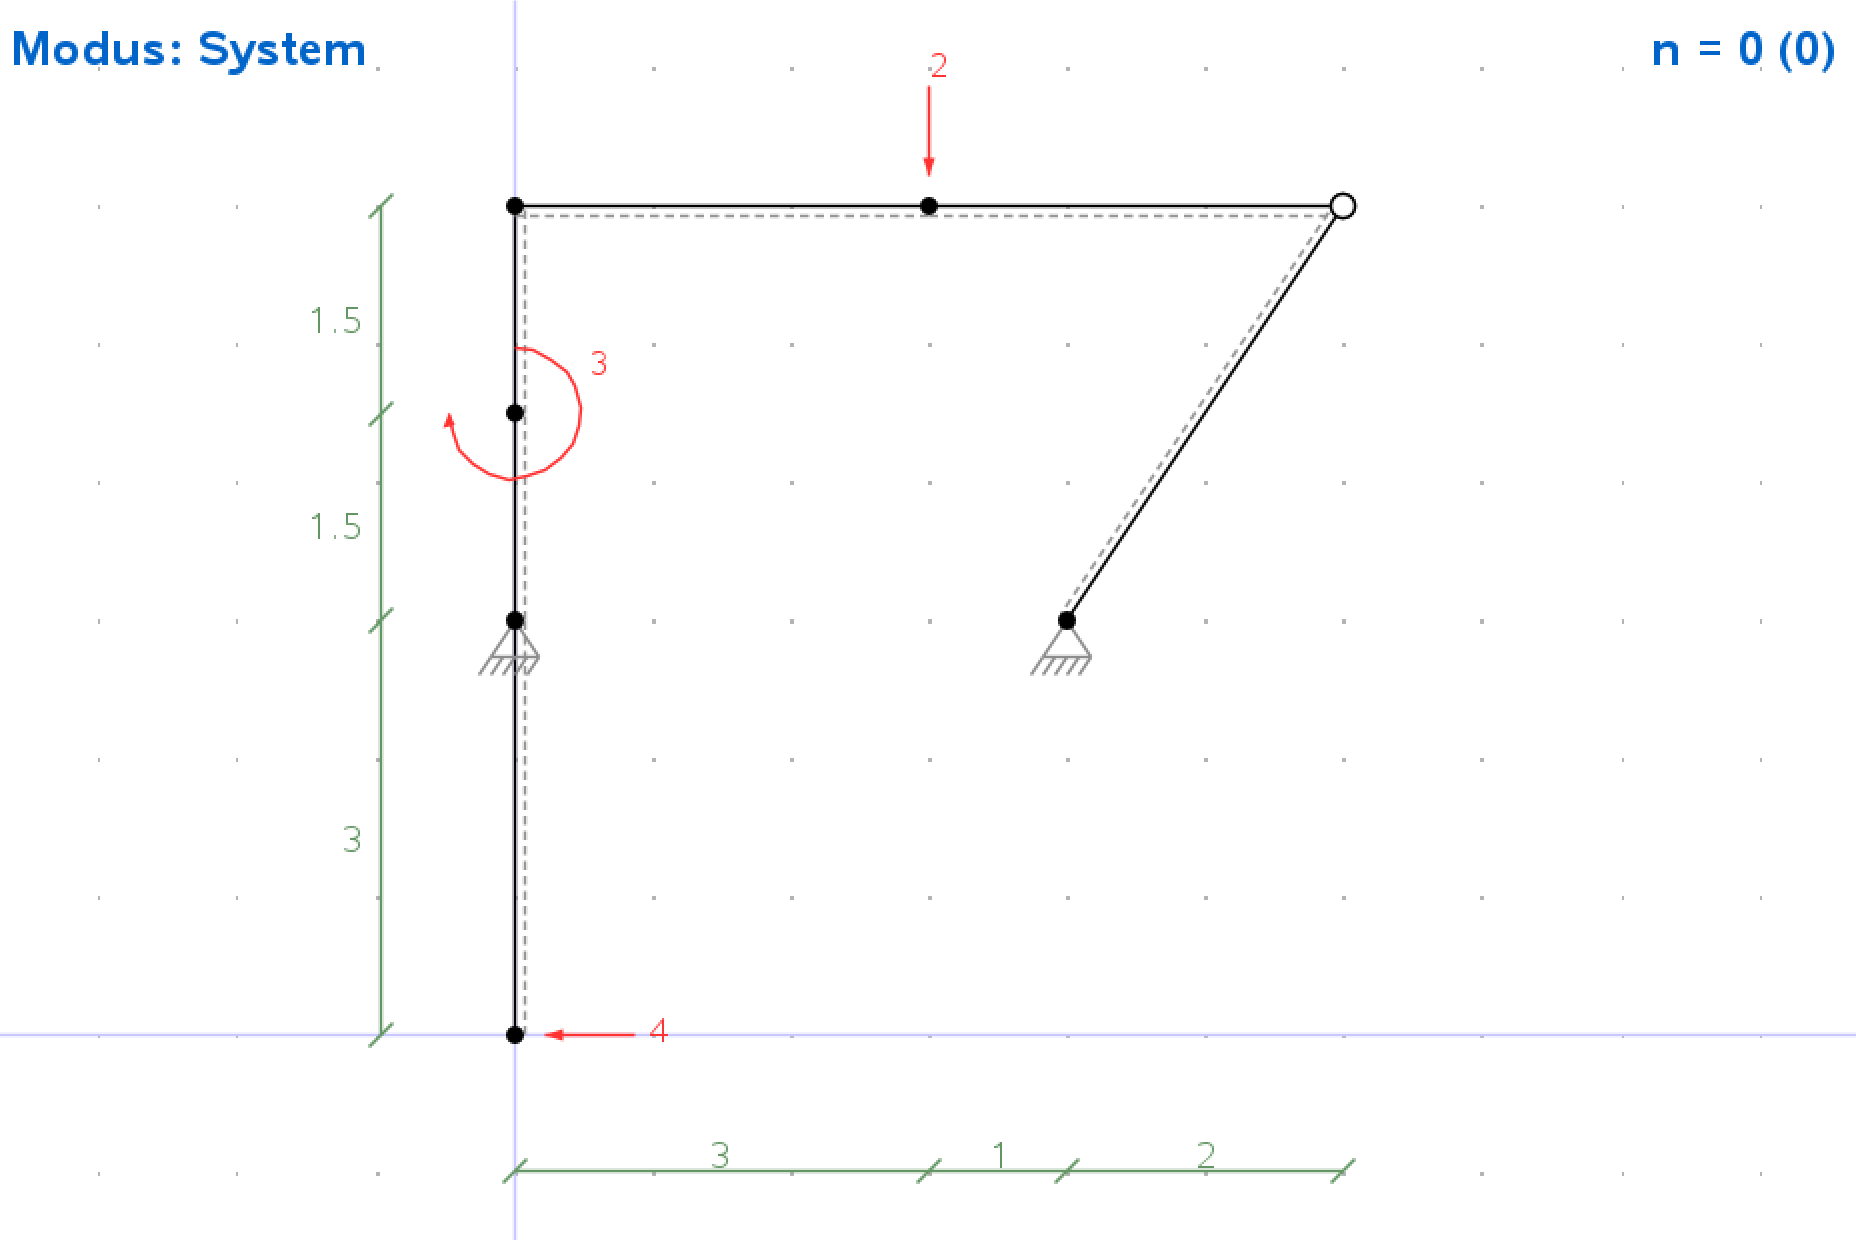
\includegraphics[width=0.5\linewidth]{./fig/TM1/WiSe2122nr3_1.png}
    \caption{TM1 WiSe~21/22, Nr.~3 im Programm}
    \label{fig:TM1WiSe2122Nr3_1}
\end{figure}

\begin{figure}[htbp]
    \centering
    \begin{subfigure}[t]{0.48\textwidth}
        \centering
        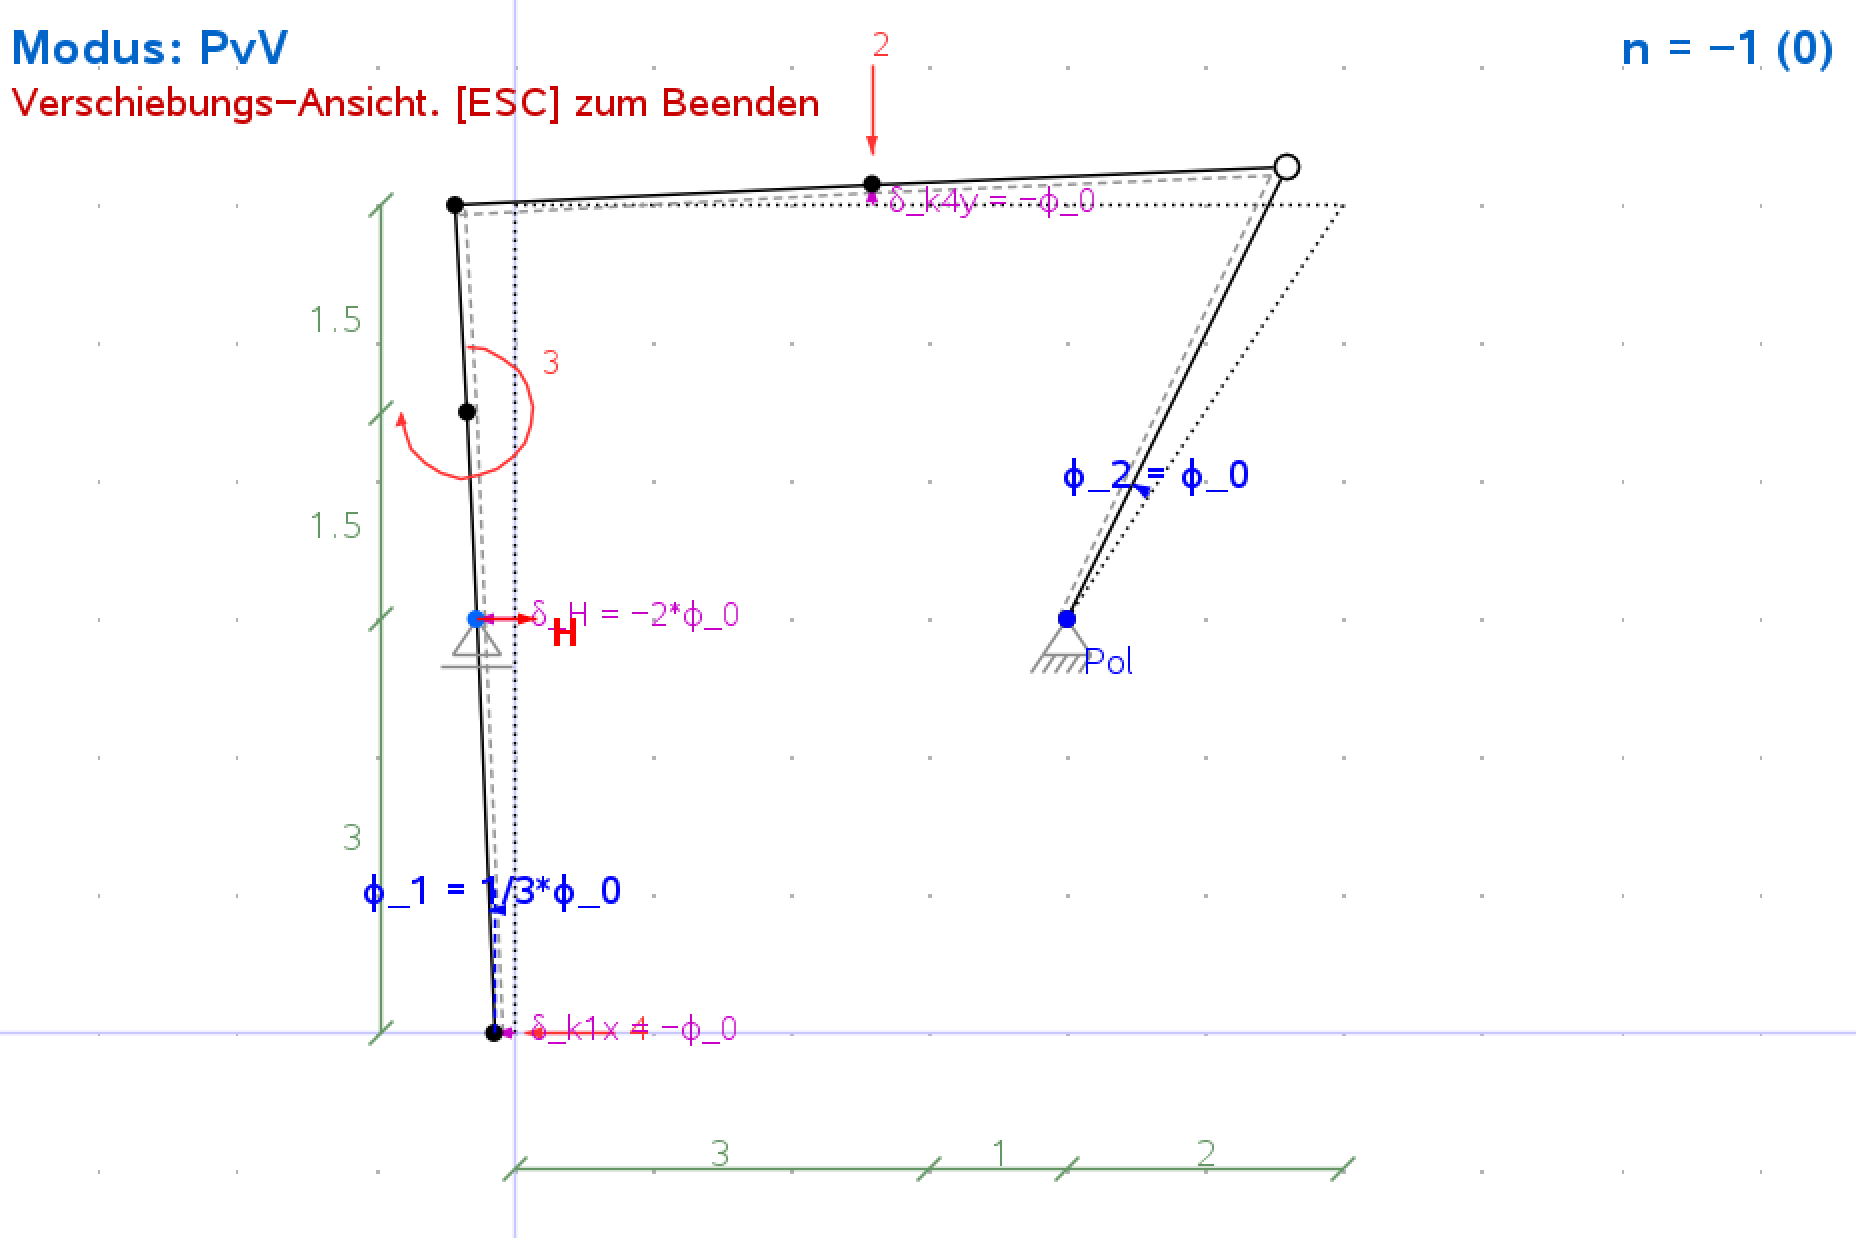
\includegraphics[width=\linewidth]{./fig/TM1/WiSe2122nr3_2.png}
        \caption{Verschiebungsfigur für $A_H$}
    \end{subfigure}
    \hfill
    \begin{subfigure}[t]{0.48\textwidth}
        \centering
        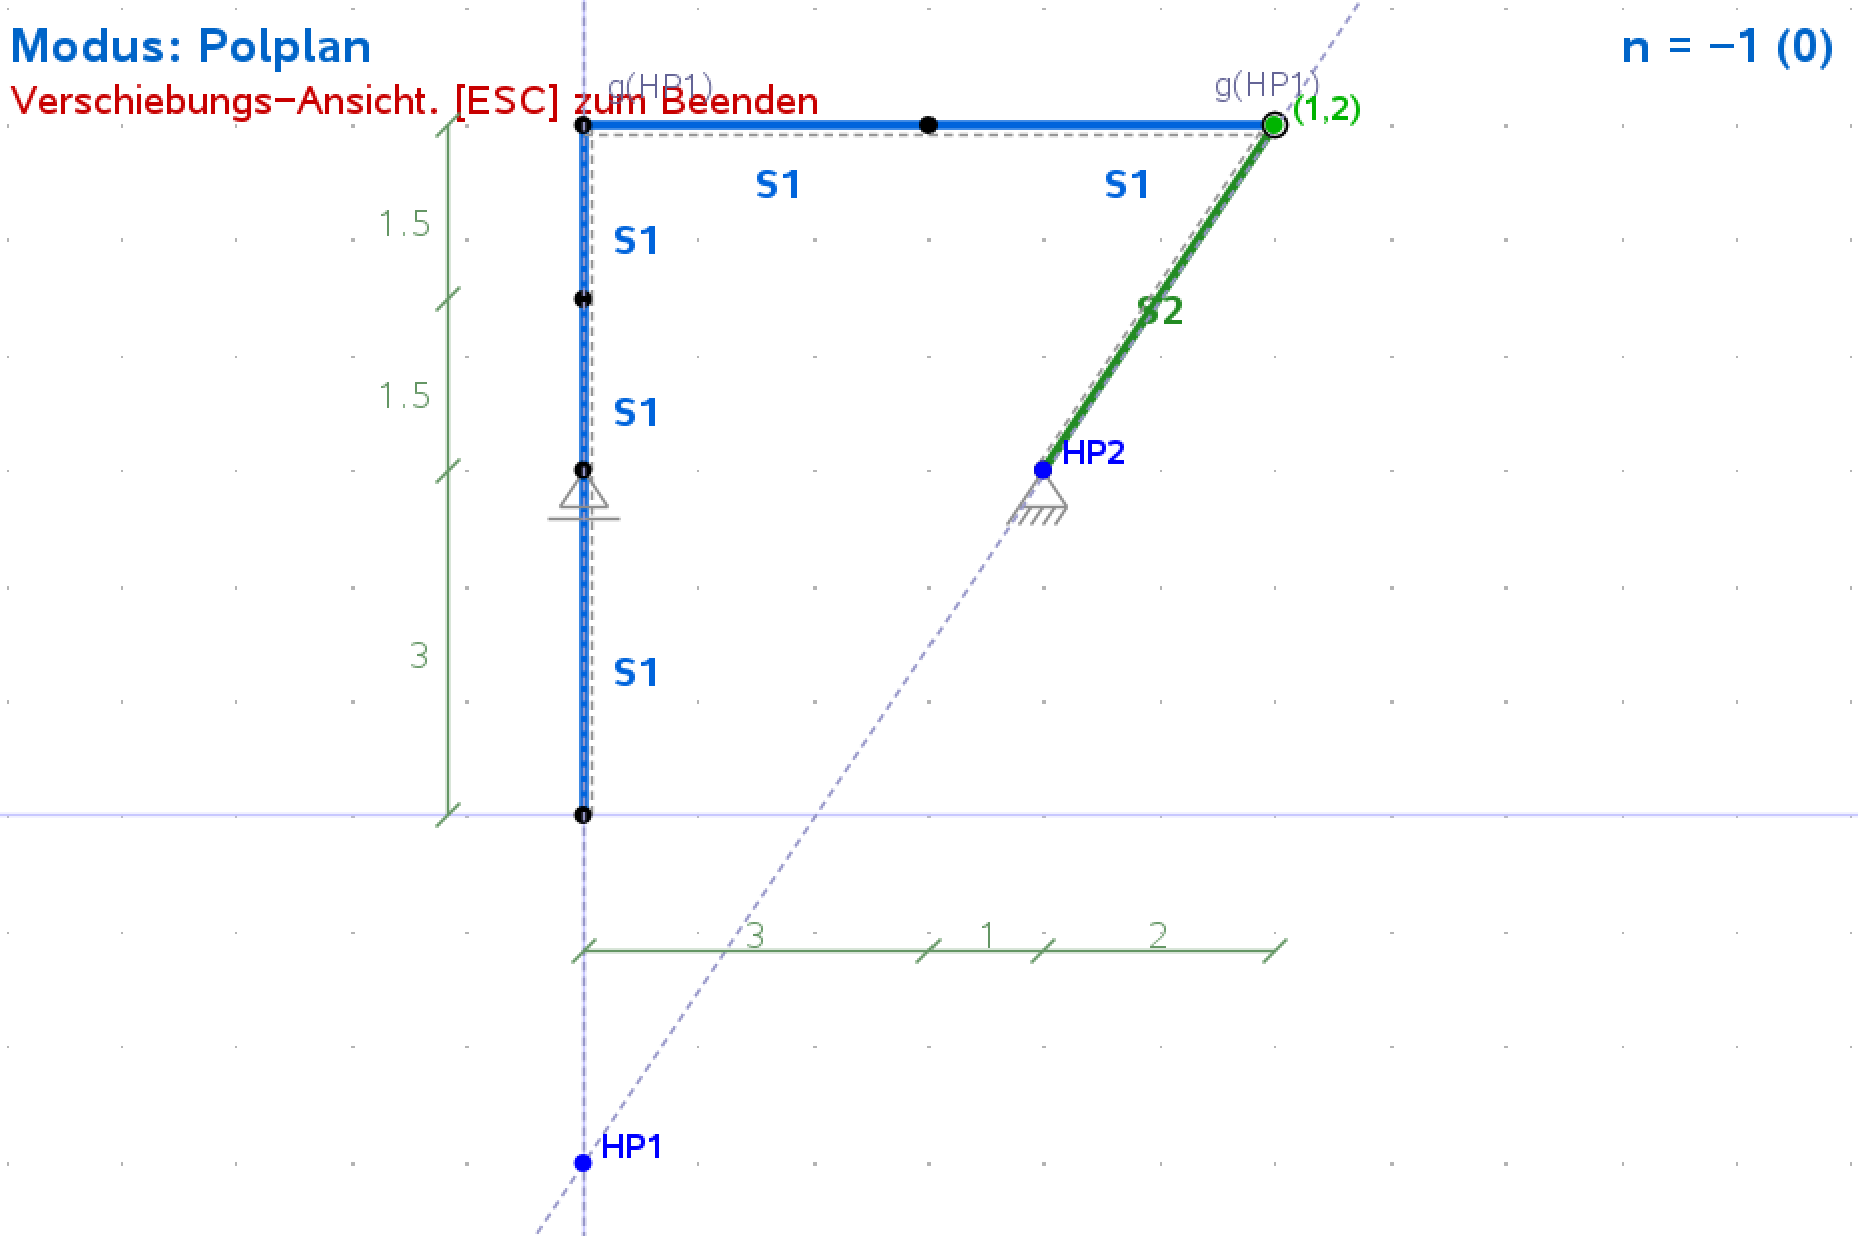
\includegraphics[width=\linewidth]{./fig/TM1/WiSe2122nr3_3.png}
        \caption{Polplan für $A_H$}
    \end{subfigure}
    \caption{WiSe~21/22, Nr.~3: $A_H$}
    \label{fig:TM1WiSe2122Nr3_2}
\end{figure}

\begin{figure}[htbp]
    \centering
    \begin{subfigure}[t]{0.48\textwidth}
        \centering
        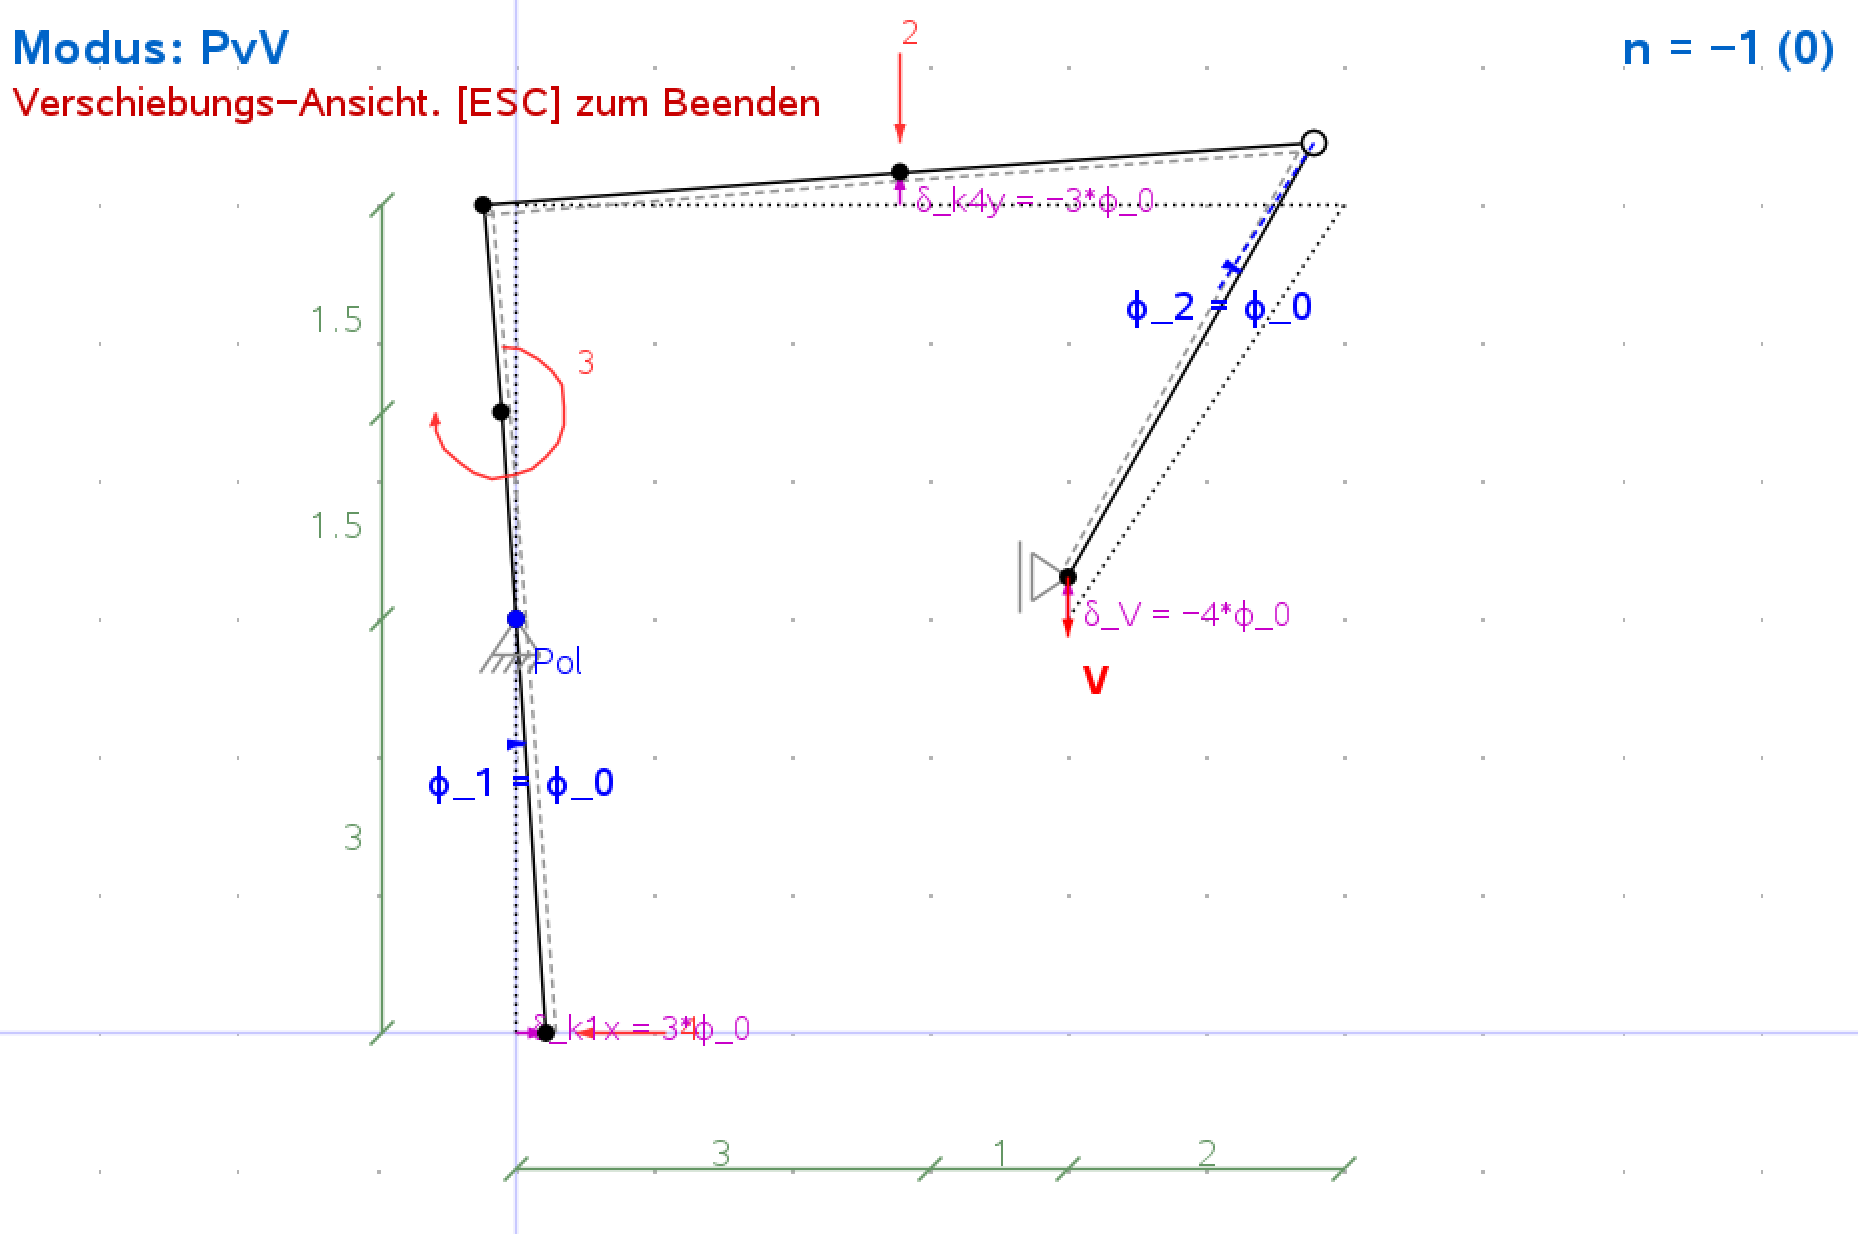
\includegraphics[width=\linewidth]{./fig/TM1/WiSe2122nr3_4.png}
        \caption{Verschiebungsfigur für $B_V$}
    \end{subfigure}
    \hfill
    \begin{subfigure}[t]{0.48\textwidth}
        \centering
        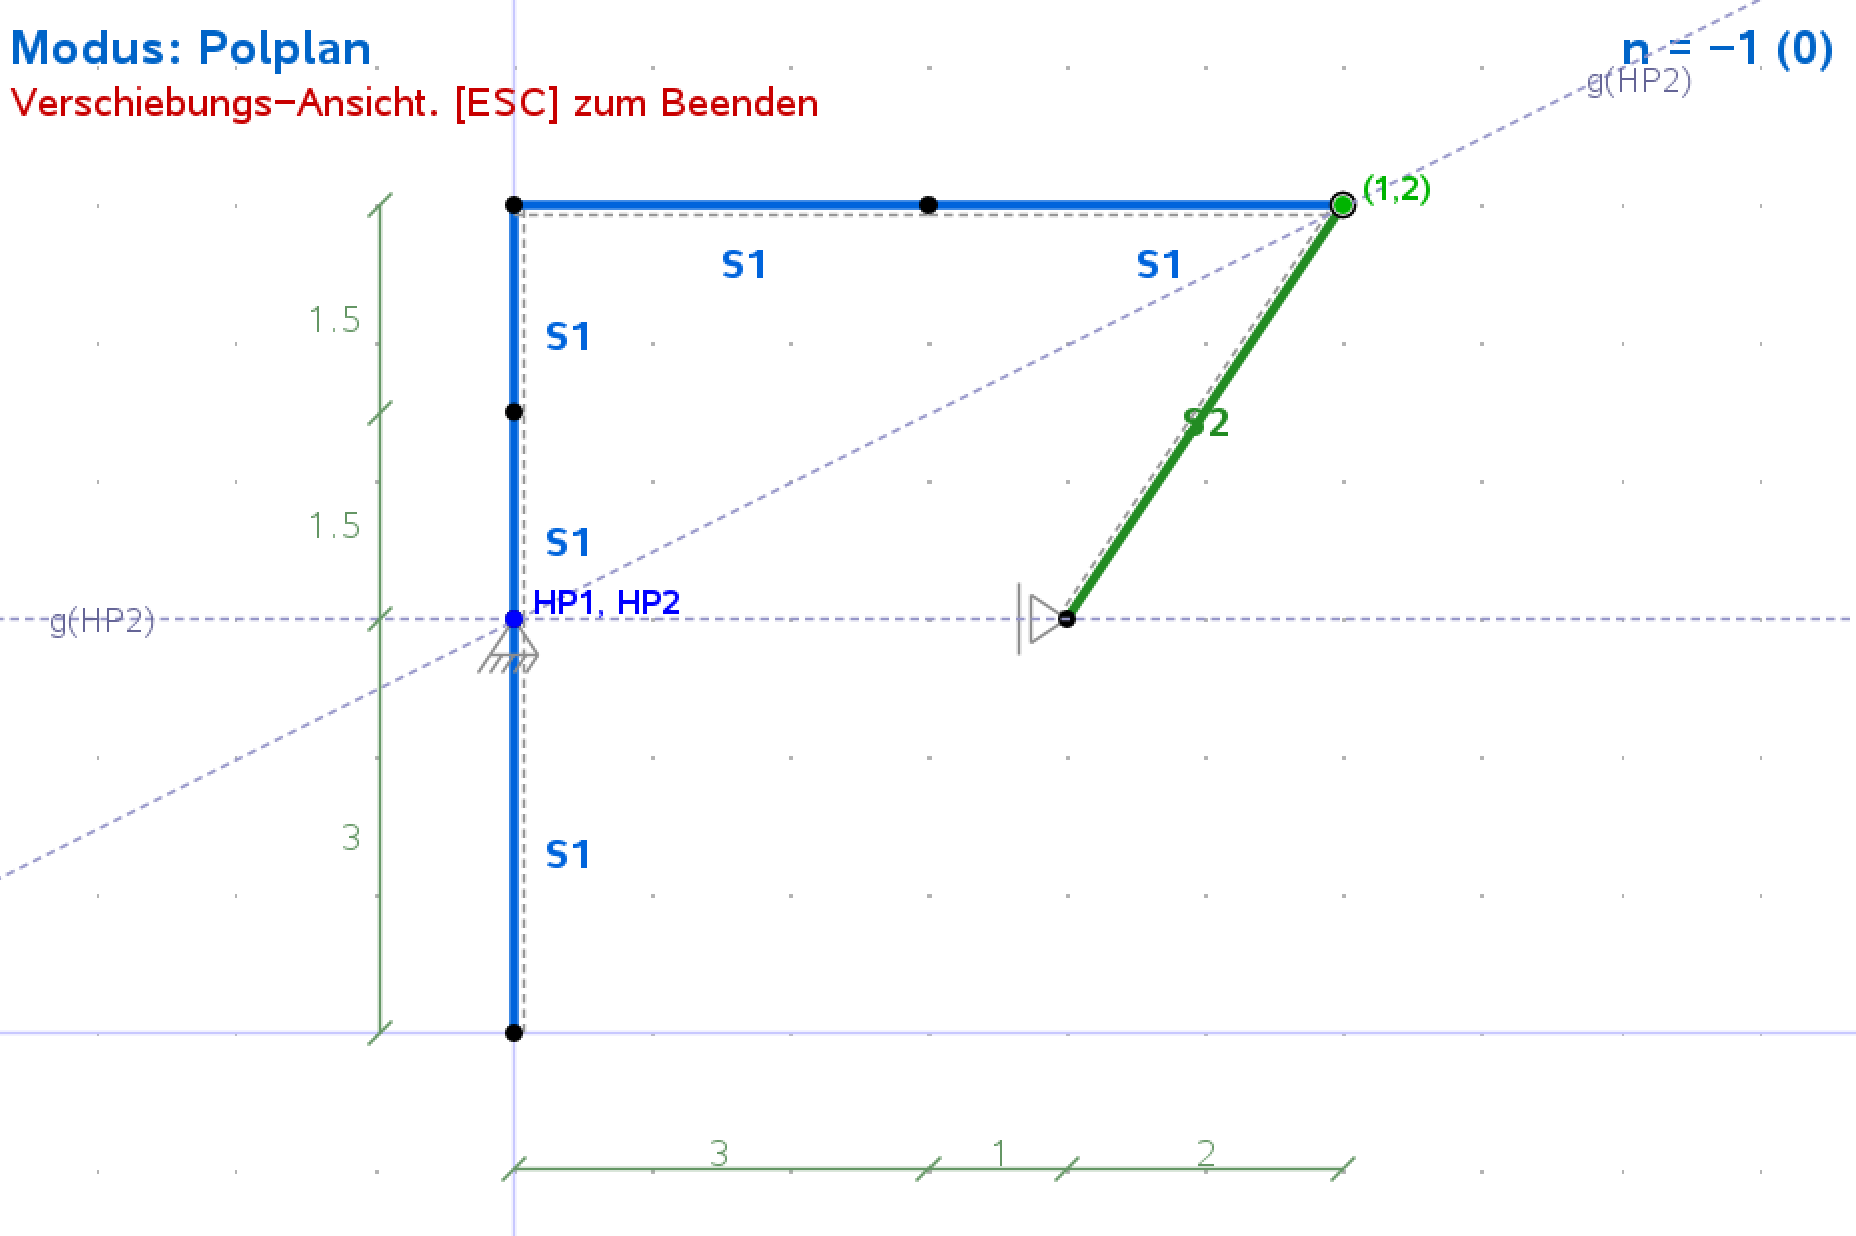
\includegraphics[width=\linewidth]{./fig/TM1/WiSe2122nr3_5.png}
        \caption{Polplan für $B_V$}
    \end{subfigure}
    \caption{WiSe~21/22, Nr.~3: $B_V$}
    \label{fig:TM1WiSe2122Nr3_3}
\end{figure}

Die Zeilen der Matrizen \code{pvv\_kin} und \code{pvv\_pol} (Abb.~\ref{fig:TM1WiSe2122Nr3_4})
sind als Gleichungskette zu lesen. Hier gilt also z.B. $\delta_{k1x}= -3\cdot\varphi_1=-\varphi_0$, oder 
$\delta x_{p12}= -9\cdot\varphi_1=-3\varphi_2$. Mit diesen Gleichungen lässt sich aus \code{w\_eq1} \code{w\_eq2} bauen.
Diese gleichung lässt sich dann entweder von hand oder mit dem Taschenrechner nach der gesuchten Größe auflösen.

\begin{figure}[htbp]
    \centering
    \begin{subfigure}[t]{0.48\textwidth}
        \centering
        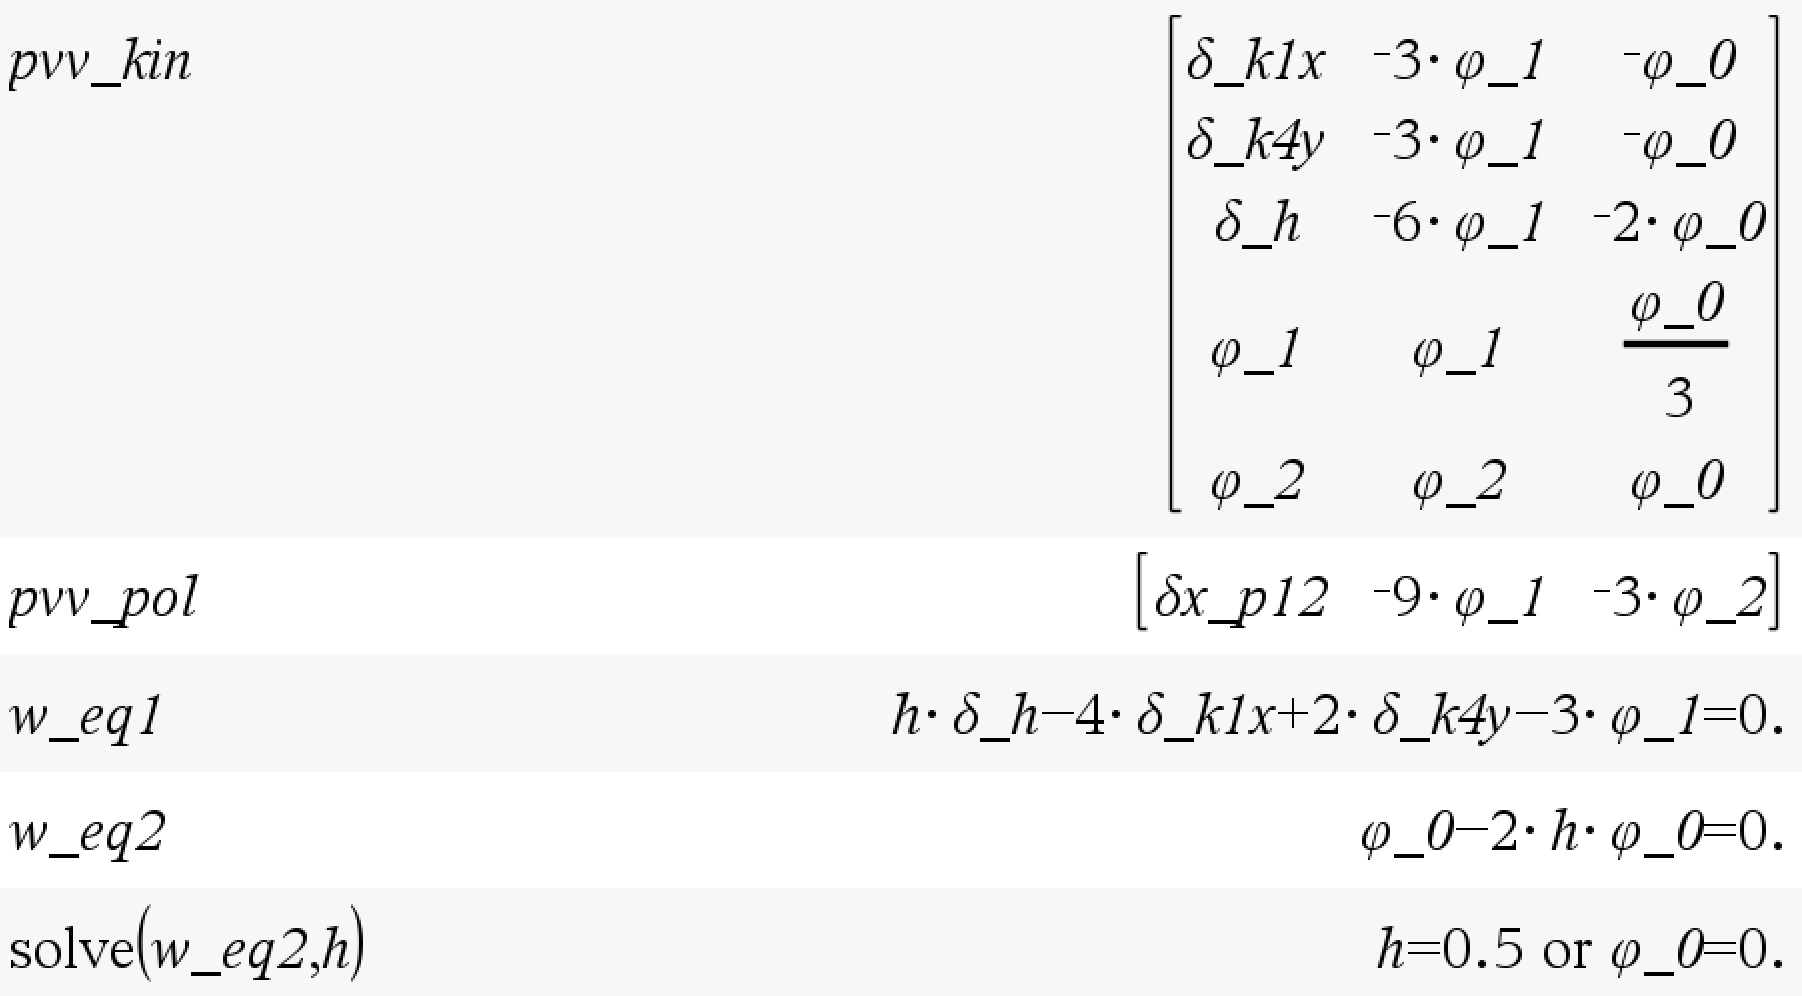
\includegraphics[width=\linewidth]{./fig/TM1/WiSe2122nr3_6.png}
        \caption{Rechnung für $A_H$}
    \end{subfigure}
    \hfill
    \begin{subfigure}[t]{0.48\textwidth}
        \centering
        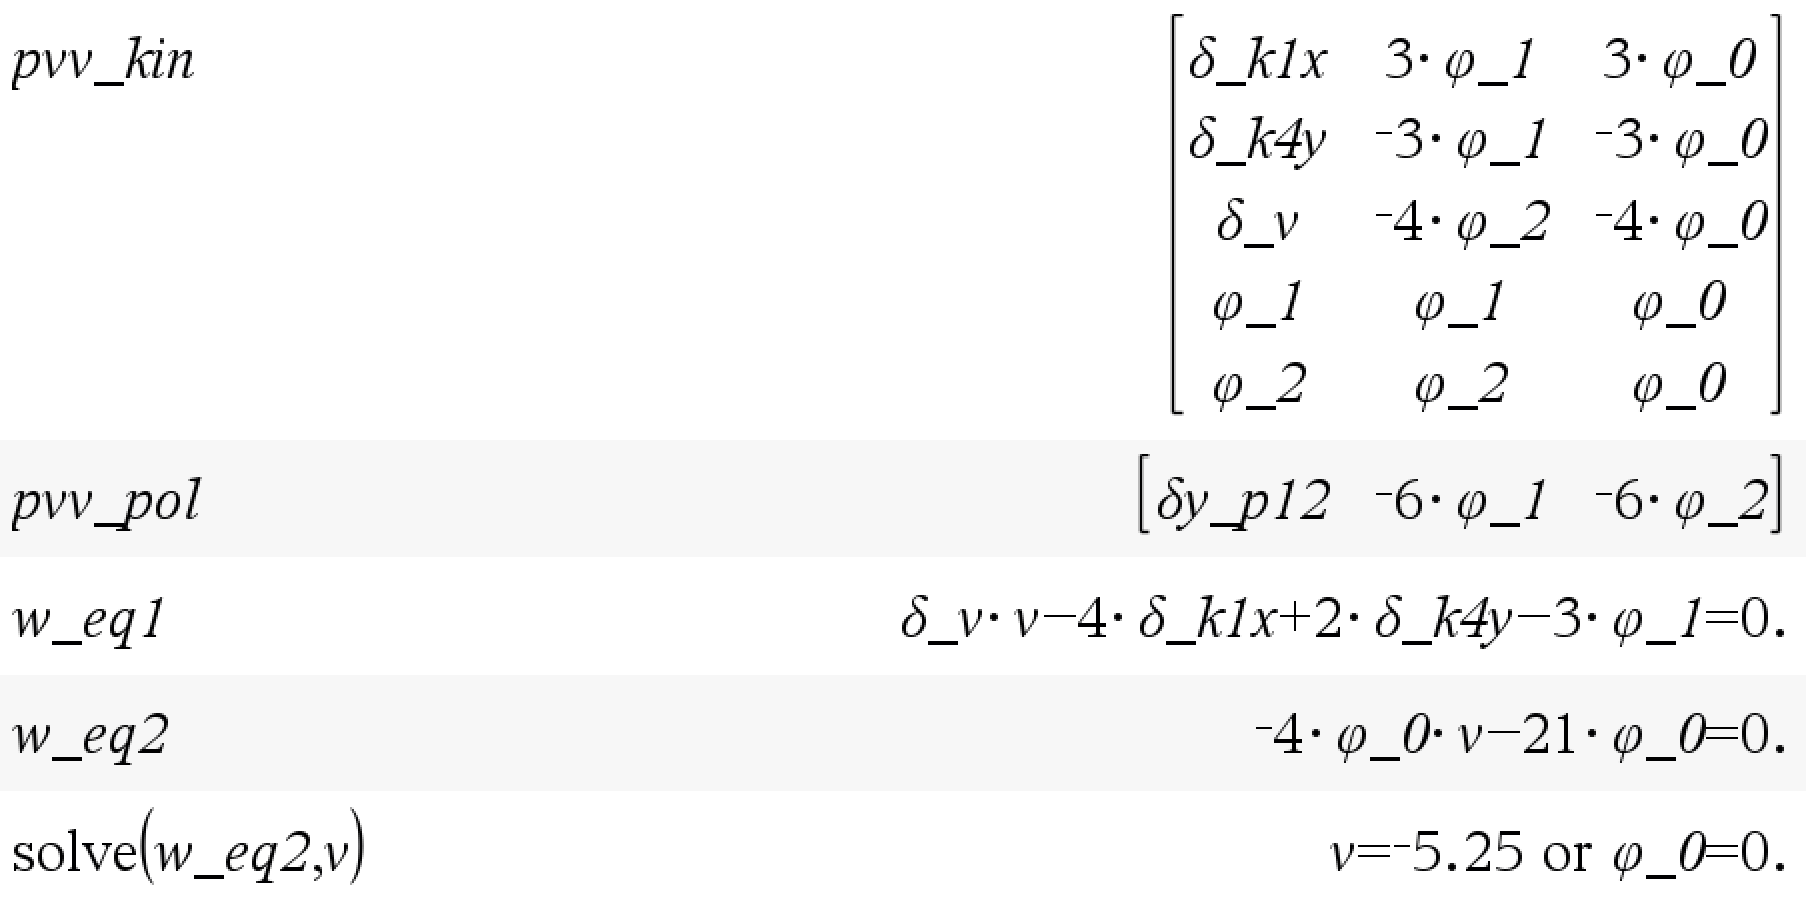
\includegraphics[width=\linewidth]{./fig/TM1/WiSe2122nr3_7.png}
        \caption{Rechnung für $B_V$}
    \end{subfigure}
    \caption{WiSe~21/22, Nr.~3: Ergebnis}
    \label{fig:TM1WiSe2122Nr3_4}
\end{figure}

\subsection{Schnittkräfte Bögen (Nr.~5)}

Mit dem Programm lassen sich die Funktionen für Schnittkraftverläufe von normalen Stäben als auch von Bögen 
ausgeben. Bei bögen ist die Laufvraibale nur nicht mehr die Länge entlang des Stabes sondern der Winkel.
also für diese Aufgabe zweilmal $\varphi \in [0,\frac{\pi}{4}]$ bzw. $\varphi \in [0,90\text{°}]$. Hier ist die Winkel-Einstellung
des Taschenrechenrs wichtig.\\
Hier gilt aber auch wieder, dass das Programm das nicht wirklich so ausrechnet wie man das von Hand machen würde, sondern
es sucht eine schöne Darstellung der Anfangswerte und kombiniert diese dann zur Funktion.

\begin{figure}[htbp]
    \centering
    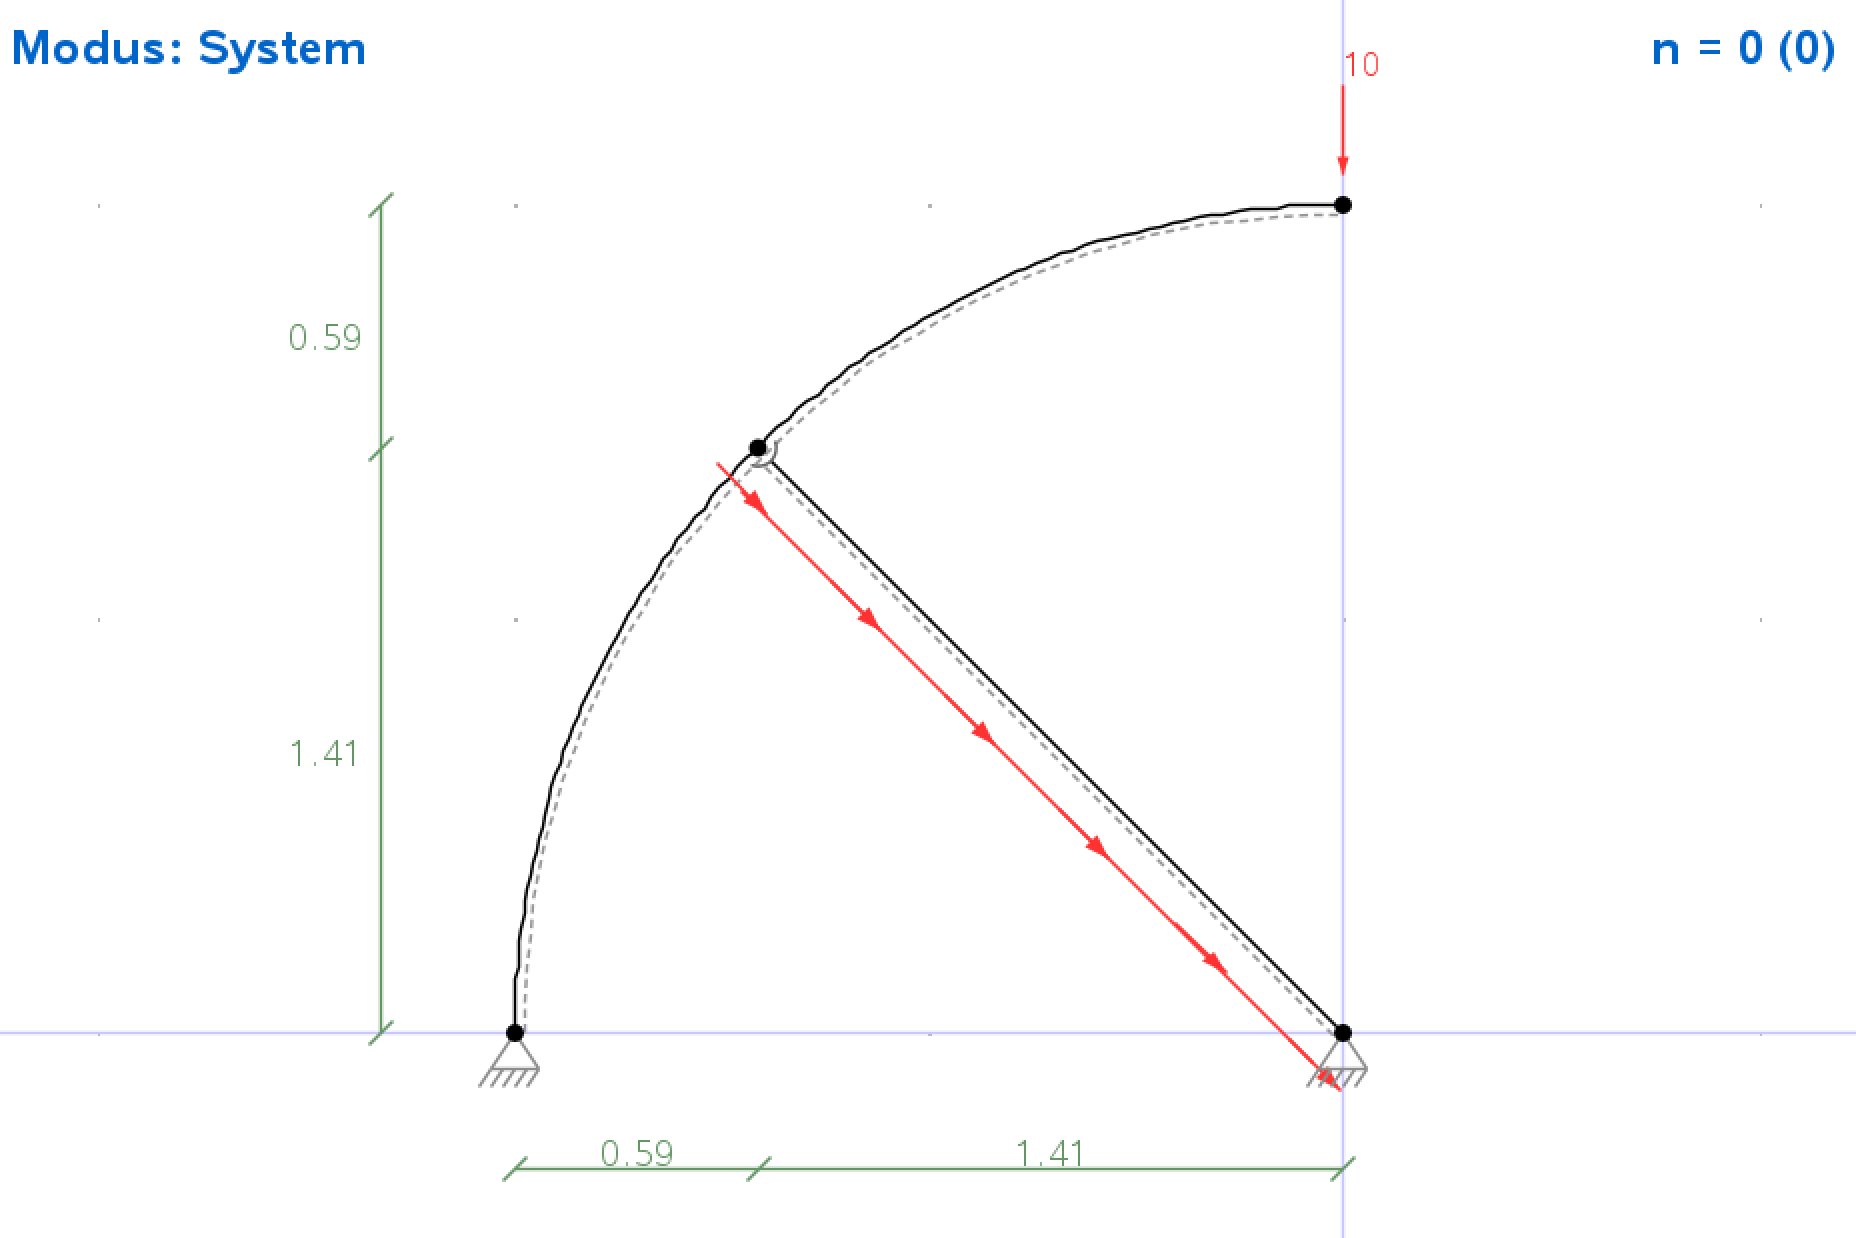
\includegraphics[width=0.5\linewidth]{./fig/TM1/WiSe2122nr5_1.png}
    \caption{TM1 WiSe~21/22, Nr.~5 im Programm}
    \label{fig:TM1WiSe2122Nr5_1}
\end{figure}


\subsection{Fachwerk (Nr.6)}

Vom Prinzip werden Fachwerke genau gleich eingegeben wie normale Systeme, nur das hier die orientierung der gestrichelten Faser
keine Rolle spielt. Es ist jedoch sinnvoll den Fachwerk Modus anzumachen, dann wird die statische Bestimmtheit beim hovern über $n=$ 
auch die Formel für Fachwerke verwendet und alle Knoten werden zu vollgelenken gemacht, auch wenn der Modus erst nach dem 
zeichnen des Systems angemacht wird.  


\begin{figure}[htbp]
    \centering
    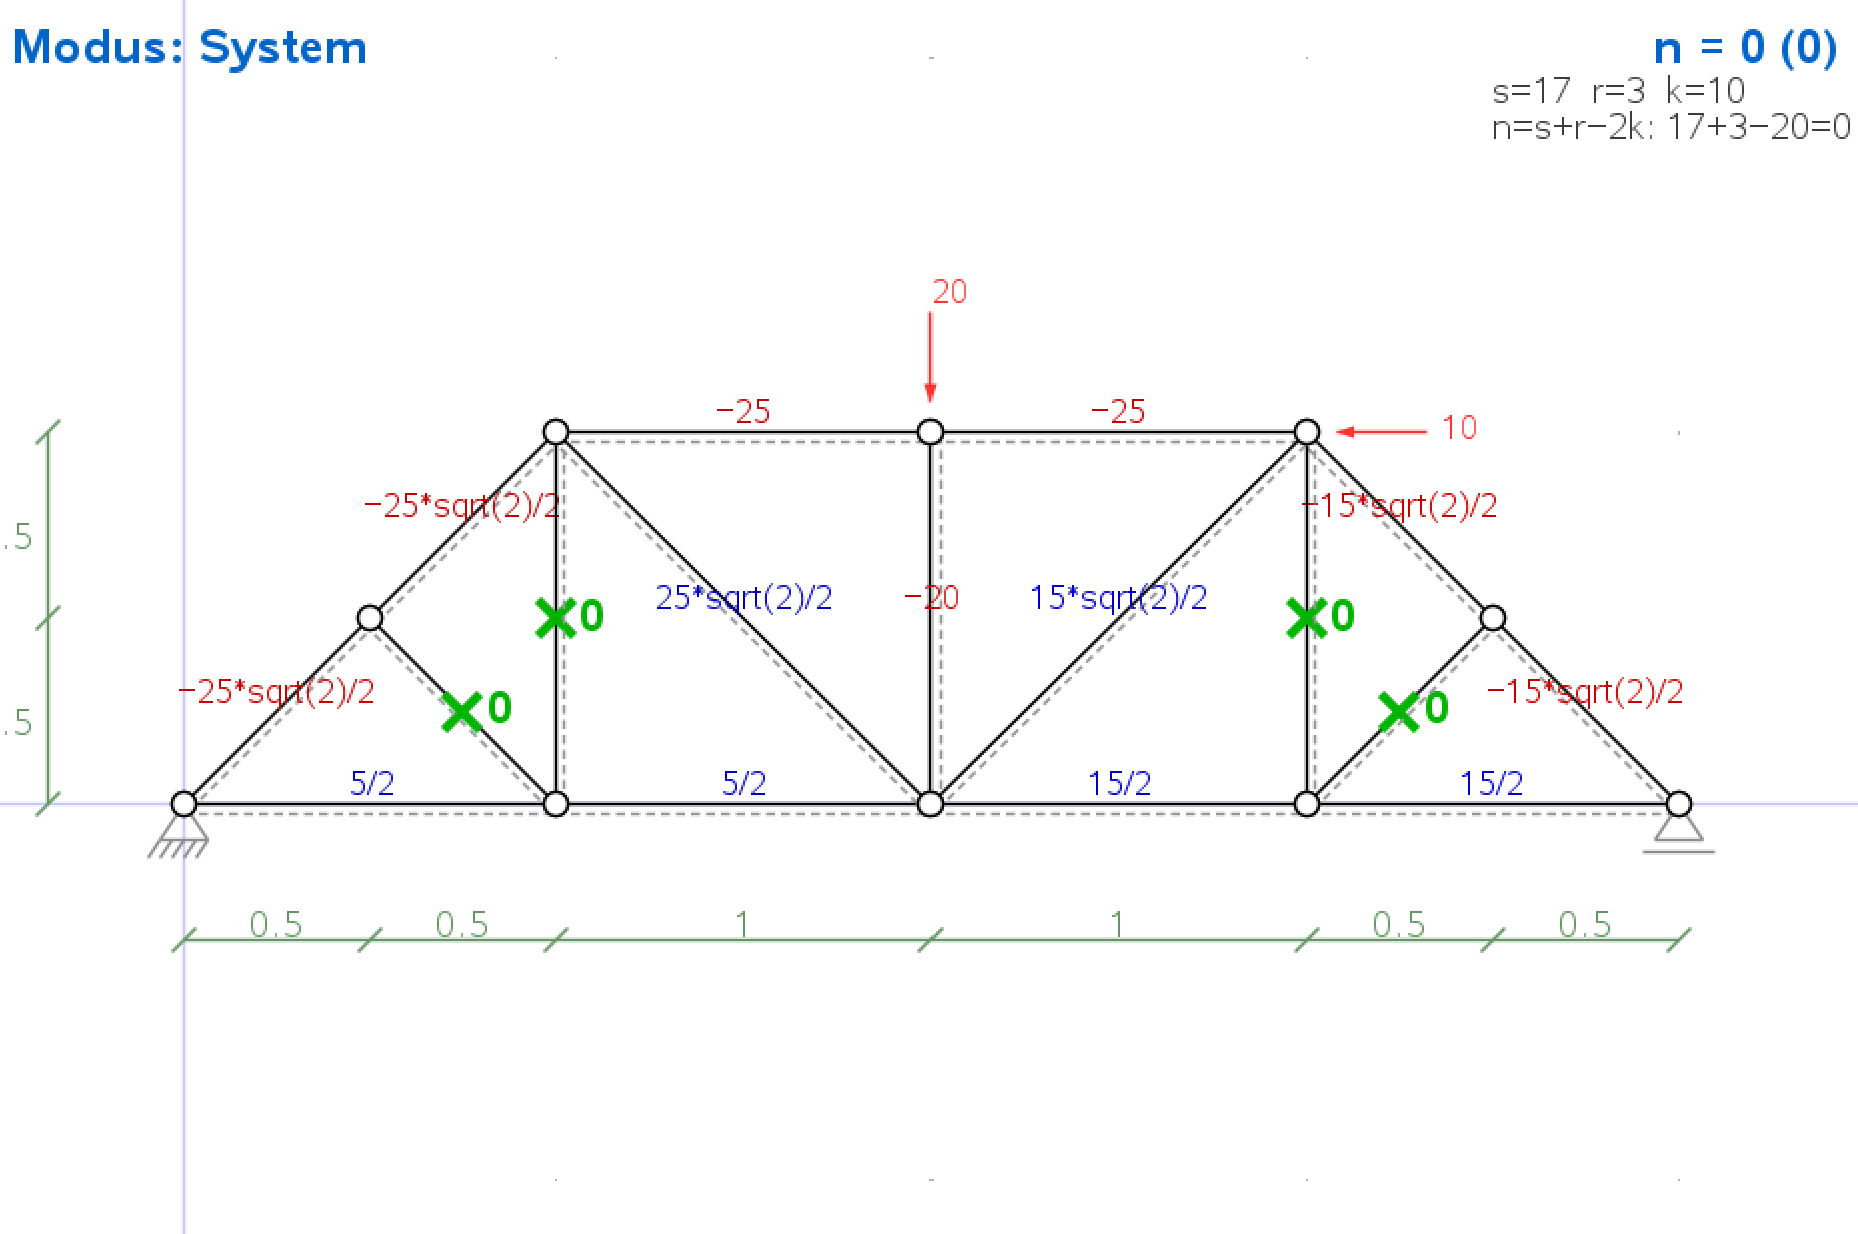
\includegraphics[width=0.5\linewidth]{./fig/TM1/WiSe2122nr6_1.png}
    \caption{TM1 WiSe~21/22, Nr.~6 im Programm}
    \label{fig:TM1WiSe2122Nr6_1}
\end{figure}

Die Stabe in Abb.~\ref{fig:TM1WiSe2122Nr6_1} die ein grünes Kreuz haben sind die ohne Rechnung erkennbaren Nullstäbe
Falls nach der Berechnung stäbkkräfte mit einer grünen Null beschriftet werdsen, aber dort kein Kreuz ist, ist das zwar ein 
Nullstab der aber nicht direkt aus den Regeln erkennbar ist. Für Afgaben bei denen nach Nullstäben gefragt wird, also nur 
die durchgekreuzten Stäbe angeben

\begin{figure}[htbp]
    \centering
    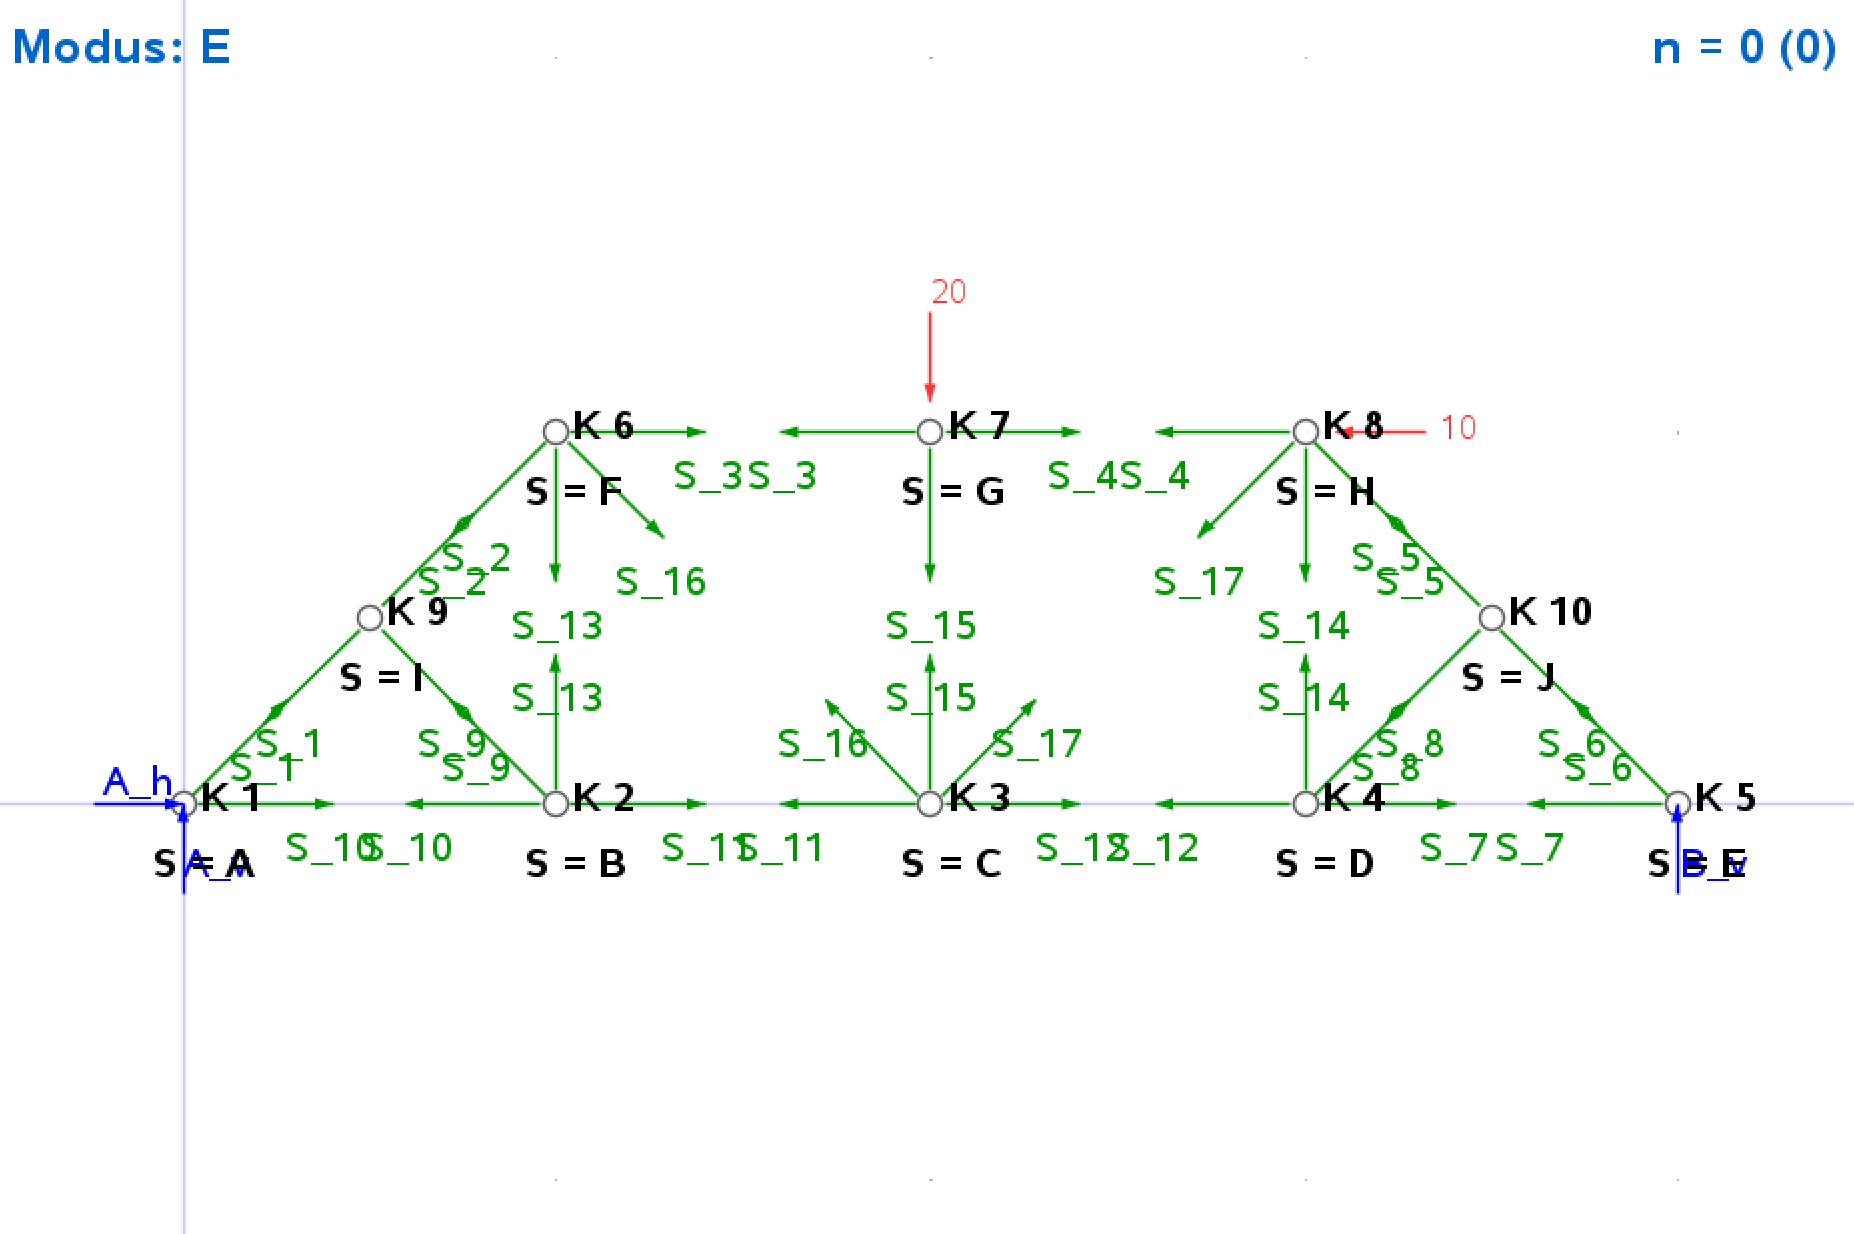
\includegraphics[width=0.5\linewidth]{./fig/TM1/WiSe2122nr6_2.png}
    \caption{TM1 WiSe~21/22 Freischnitt}
    \label{fig:TM1WiSe2122Nr6_2}
\end{figure}

Für die Verwendung der beiden Seiten des E-Modus muss darauf geachtet werden, dass entweder die Stäbe in der
gleichen Reihenfolge wie in der Aufgabe gezeichnet werden oder die Bennenung hinterher angepasst wird. Macht ihr das nicht
ist z.B. Stab 13 aus eurer Rechnung nicht Stab 13 aus der Aufgabe\\
Gleiches gilt natürlich auch für die Verwendung des LGS-Exports. Hier wird (Falls der Fachwerk Modus an ist) 
das Knotenschnittverfahren verwendet. Die Benennung im LGS ist die gleiche wie auf der zweiten Seite des E-Modus.





\section{TM2}

\subsection{Biegelinie (TM2 WiSe~21/22, Nr.~7)} \label{ex:Biegelinienaufgabe}

In dieser Aufgabe ist ein \emph{interessantes} KOS vorgegeben: Soll es ein Rechtssystem sein,
zeigt die $y$-Achse hier in die Zeichenebene hinein und nicht, wie sonst üblich, aus ihr heraus.

Rechnet ihr von Hand über die DGL $EI\,w'''' = q$ mit allen Rand- und Übergangsbedingungen (so
geht man bei statisch unbestimmten Systemen meist vor, und so rechnet auch \code{wneu}), gibt es
hier nichts weiter zu beachten. Bei einem statisch bestimmten System lohnt es sich dagegen, zuerst
die Momentenlinie zu berechnen und dann $EI\,w'' = -M$ zu integrieren. Dafür braucht ihr die
gestrichelte Faser. Die Regel aus Abschnitt~\ref{sec:Eingabe_Stäbe}, dass sie immer auf der Seite
liegt, in die die $z$- bzw.\ $w$-Achse zeigt, gilt auch hier. Alternativ könnt ihr euch überlegen,
auf welcher Seite ein positives Schnittmoment $M_y$ (Drehsinn nach der Rechte-Hand-Regel um die
$y$-Achse) Zug erzeugt, dort liegt die gestrichelte Faser. Das finde ich aber umständlicher.

Im Programm müsst ihr solche Systeme etwas anders eingeben, denn dort zeigt die $y$-Achse immer
aus der Zeichenebene heraus. Zeichnet ihr das System genau wie in der Aufgabe und setzt die
gestrichelte Faser nach der Regel oben, läuft die $x$-Koordinate im Programm in die andere Richtung
als in der Aufgabe. Um das zu umgehen, zeichnet ihr Systeme, bei denen die $y$-Achse in die
Zeichenebene hineinzeigt, spiegelverkehrt (Abb.~\ref{fig:Biegelinienaufgabe}). Ich habe die
Aufgabe im symbolischen Modus gerechnet, deshalb stehen in den Ergebnissen $q$ und $l$.

\begin{figure}[htbp]
    \centering
    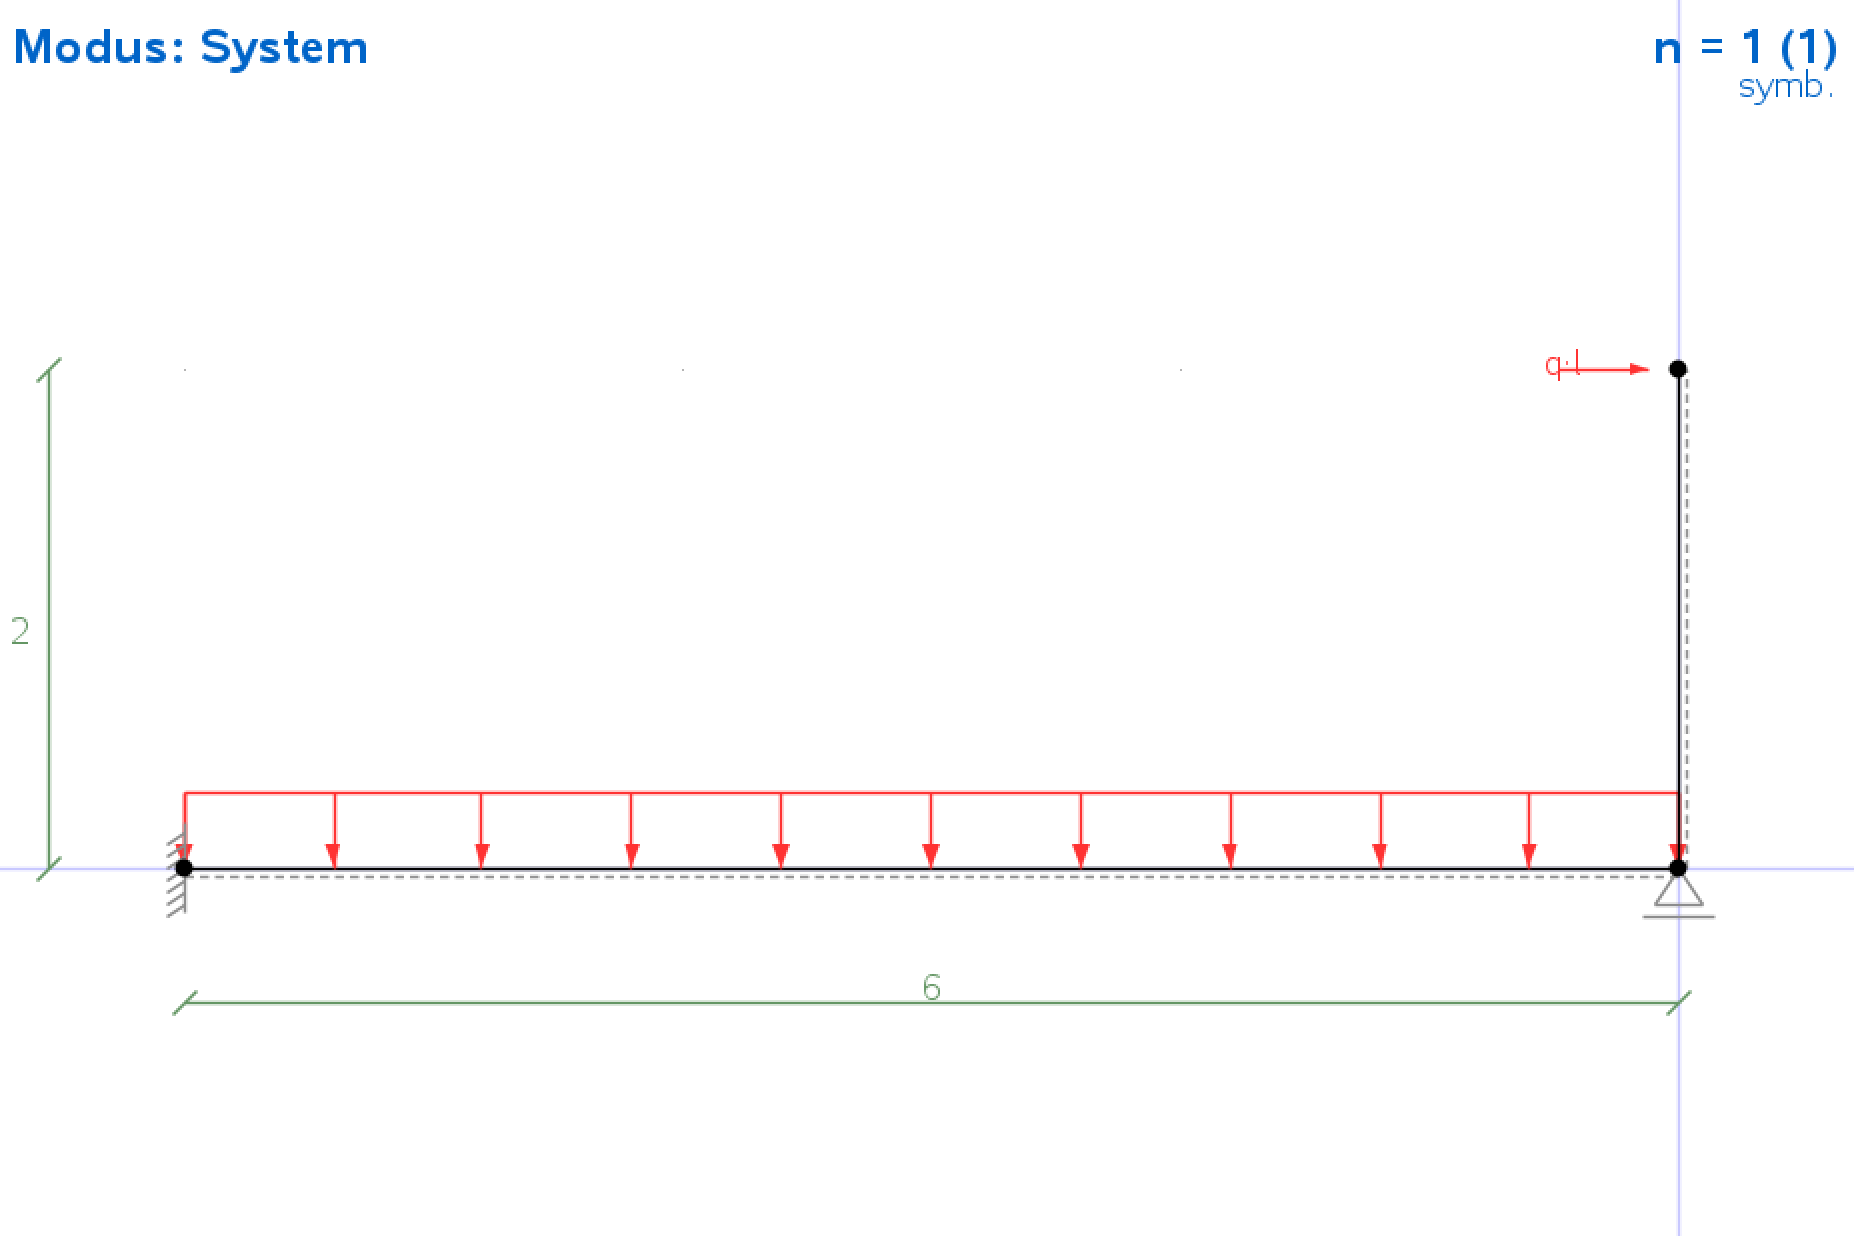
\includegraphics[width=0.5\linewidth]{./fig/TM2/WiSe2122nr7_1.png}
    \caption{TM2 WiSe~21/22, Nr.~7 im Programm, spiegelverkehrt gezeichnet}
    \label{fig:Biegelinienaufgabe}
\end{figure}

Das liefert die Ergebnisse in Abb.~\ref{fig:BiegelinienaufgabeBiegelinie}. Hier geben beide
Methoden dasselbe Ergebnis. Das sollte natürlich so sein, ist aber nicht immer so: Manchmal weicht
die WGV/FEM-Lösung \code{v\_EI\_stab1(x)} (im Rechner klein geschrieben) minimal von der exakten
Lösung \code{wneu1(x)} ab. Weil das Programm die Brüche aus den Zahlen der FEM-Lösung
\emph{errät} (Abschnitt~\ref{sec:mathe-symbolisch}), kann daraus eine ganz anders aussehende
Biegelinie werden. Die Methode über die WGV/FEM-Lösung gibt es trotzdem, vor allem weil ich sie
zuerst programmiert habe (daher wohl auch der Name \code{wneu} der anderen Funktion), und weil sie
bei sehr großen Systemen deutlich schneller sein kann.

\begin{figure}[htbp]
    \centering
    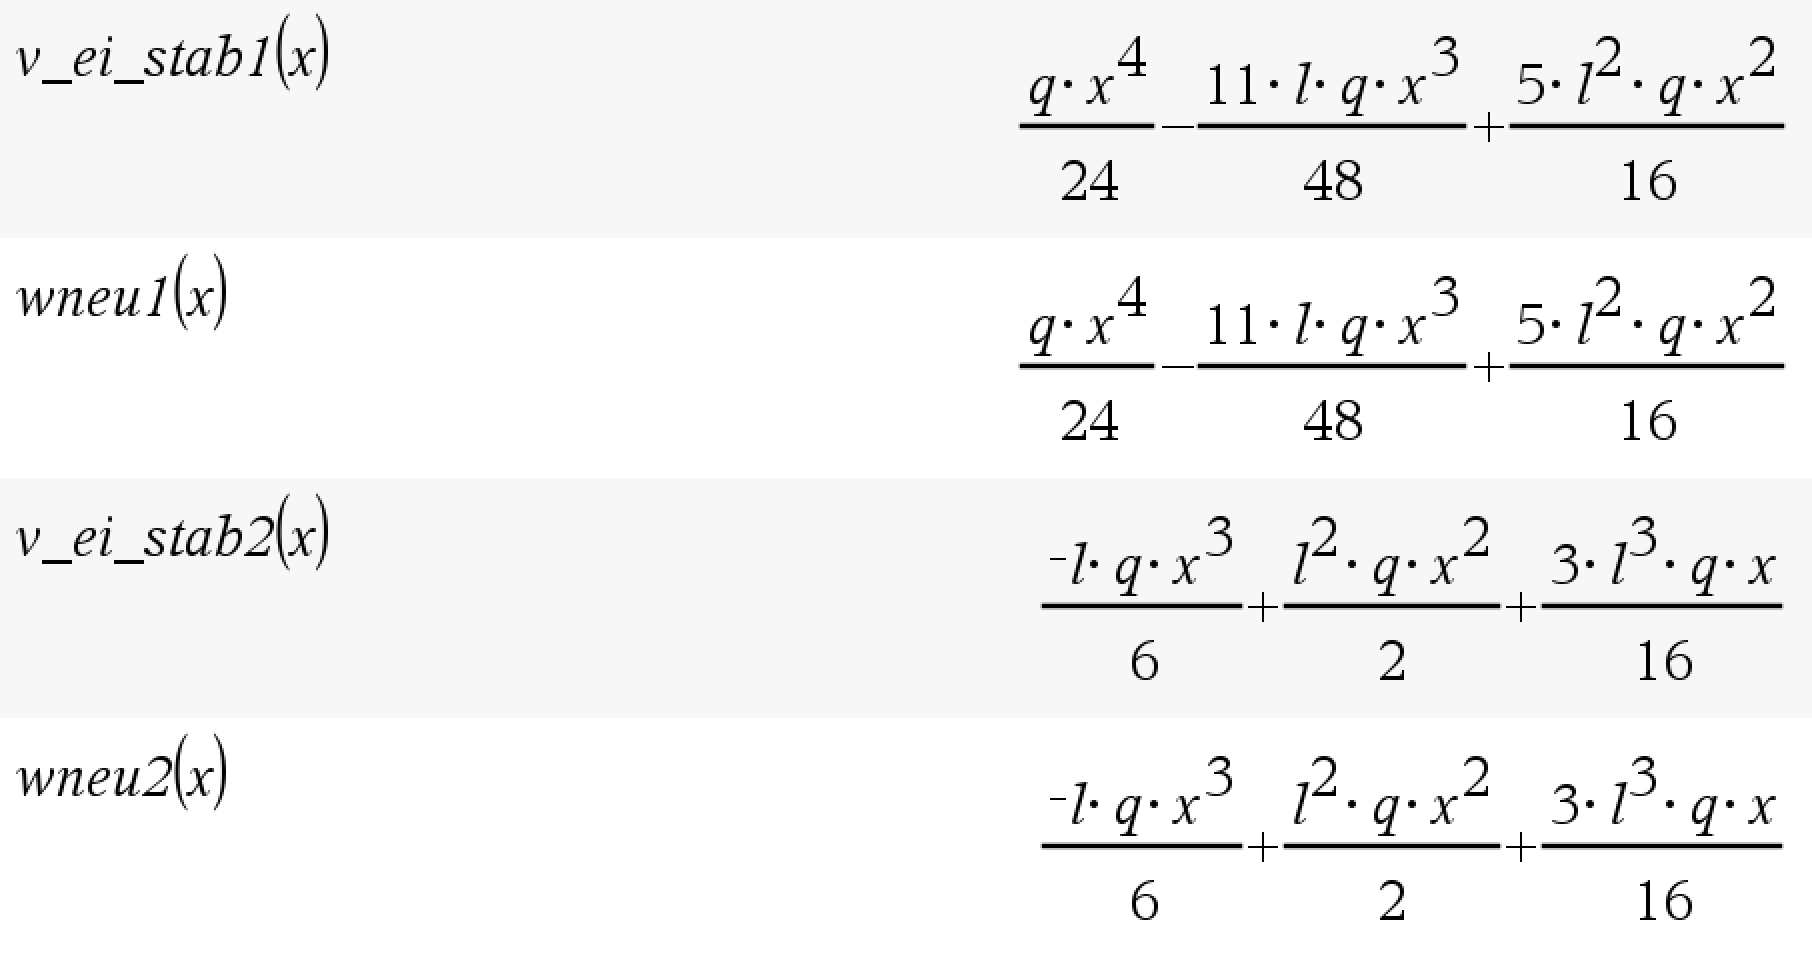
\includegraphics[width=0.5\linewidth]{./fig/TM2/WiSe2122nr7_2.png}
    \caption{TM2 WiSe~21/22, Nr.~7: \code{v\_EI\_stab} und \code{wneu} im Vergleich}
    \label{fig:BiegelinienaufgabeBiegelinie}
\end{figure}

Weil die Stäbe dehnsteif sind, kann das Programm hier sogar die Randbedingungen für Biegelinie und
Längslinie getrennt angeben (Abb.~\ref{fig:BiegelinienaufgabeRandbed}): Die Bedingungen im oberen
Block reichen für die Biegelinie allein, die im unteren kommen nur für die Längslinie dazu. Das geht
nicht immer. Sind die Stäbe dehnbar, hängt die Biegelinie über die Rahmenecken auch von den
Längsverformungen ab, und das Programm gibt alle Bedingungen zusammen aus
(Abschnitt~\ref{sec:randlgs}).

\begin{figure}[htbp]
    \centering
    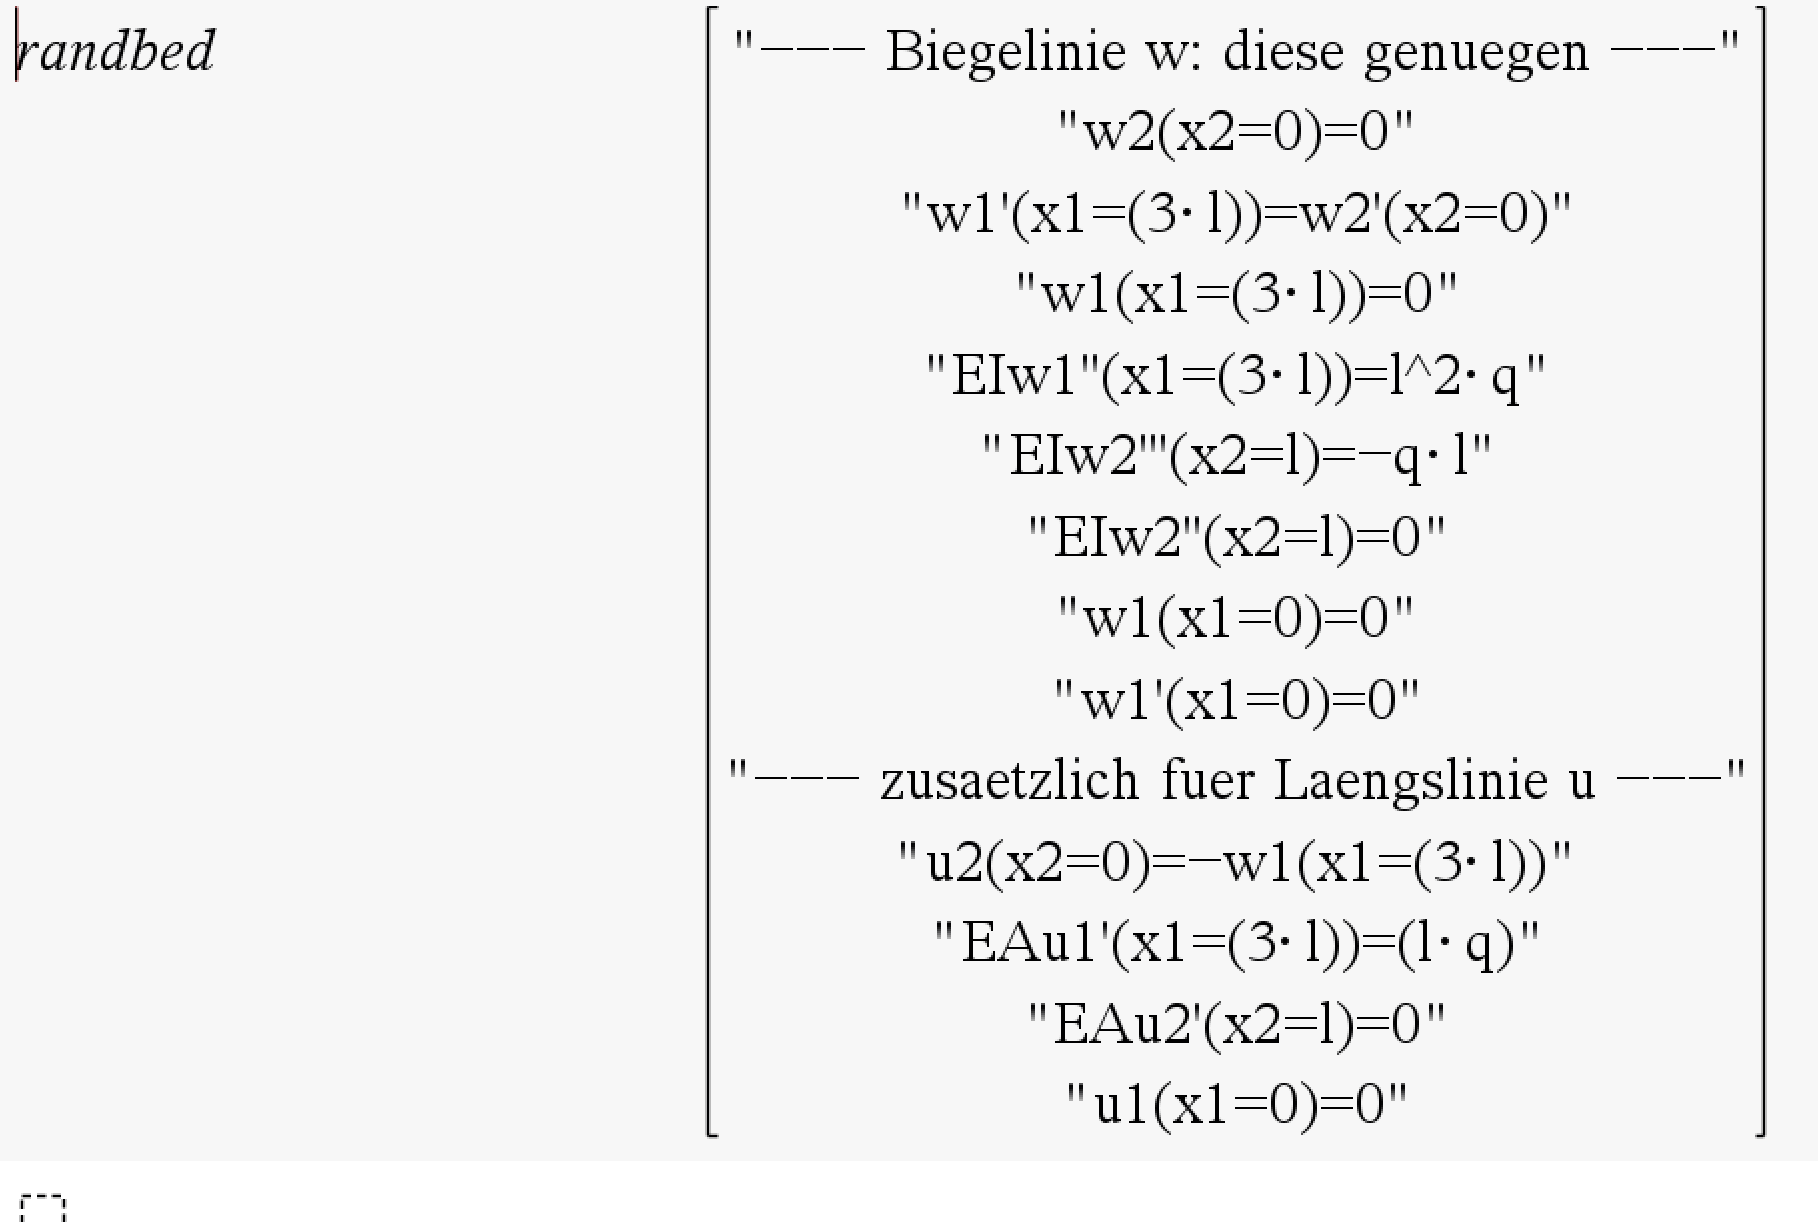
\includegraphics[width=0.5\linewidth]{./fig/TM2/WiSe2122nr7_3.png}
    \caption{Randbedingungen \code{randbed} für TM2 WiSe~21/22, Nr.~7}
    \label{fig:BiegelinienaufgabeRandbed}
\end{figure}



\subsection{Verschiebungsaufgaben (TM2 WiSe~20/21 Nr.~4)} \label{ex:Temperaturaufgabe}

Aufgaben wie diese lassen sich mit der richtigen Eingabe auch direkt im Programm lösen. Wie diese Aufagbe im
Programm aussieht ist in Abb.~\ref{fig:verschiebungSystem} dargestellt. Hierbei muss natürlich auf die Einheiten geachtet werden.
In der Aufgabe sind die relevanten Dehnsteifigkeiten nicht direkt gegeben, genauso wie manche Angaben nicht in der
für das Programm geforderten Einheit sind.\\
Für Kräfte immer kN, genauso wie für die Dehnsteifigkeit $EA$ und die Biegesteifigkeit $EI$ in kNm.  

\begin{figure}[htbp]
    \centering
    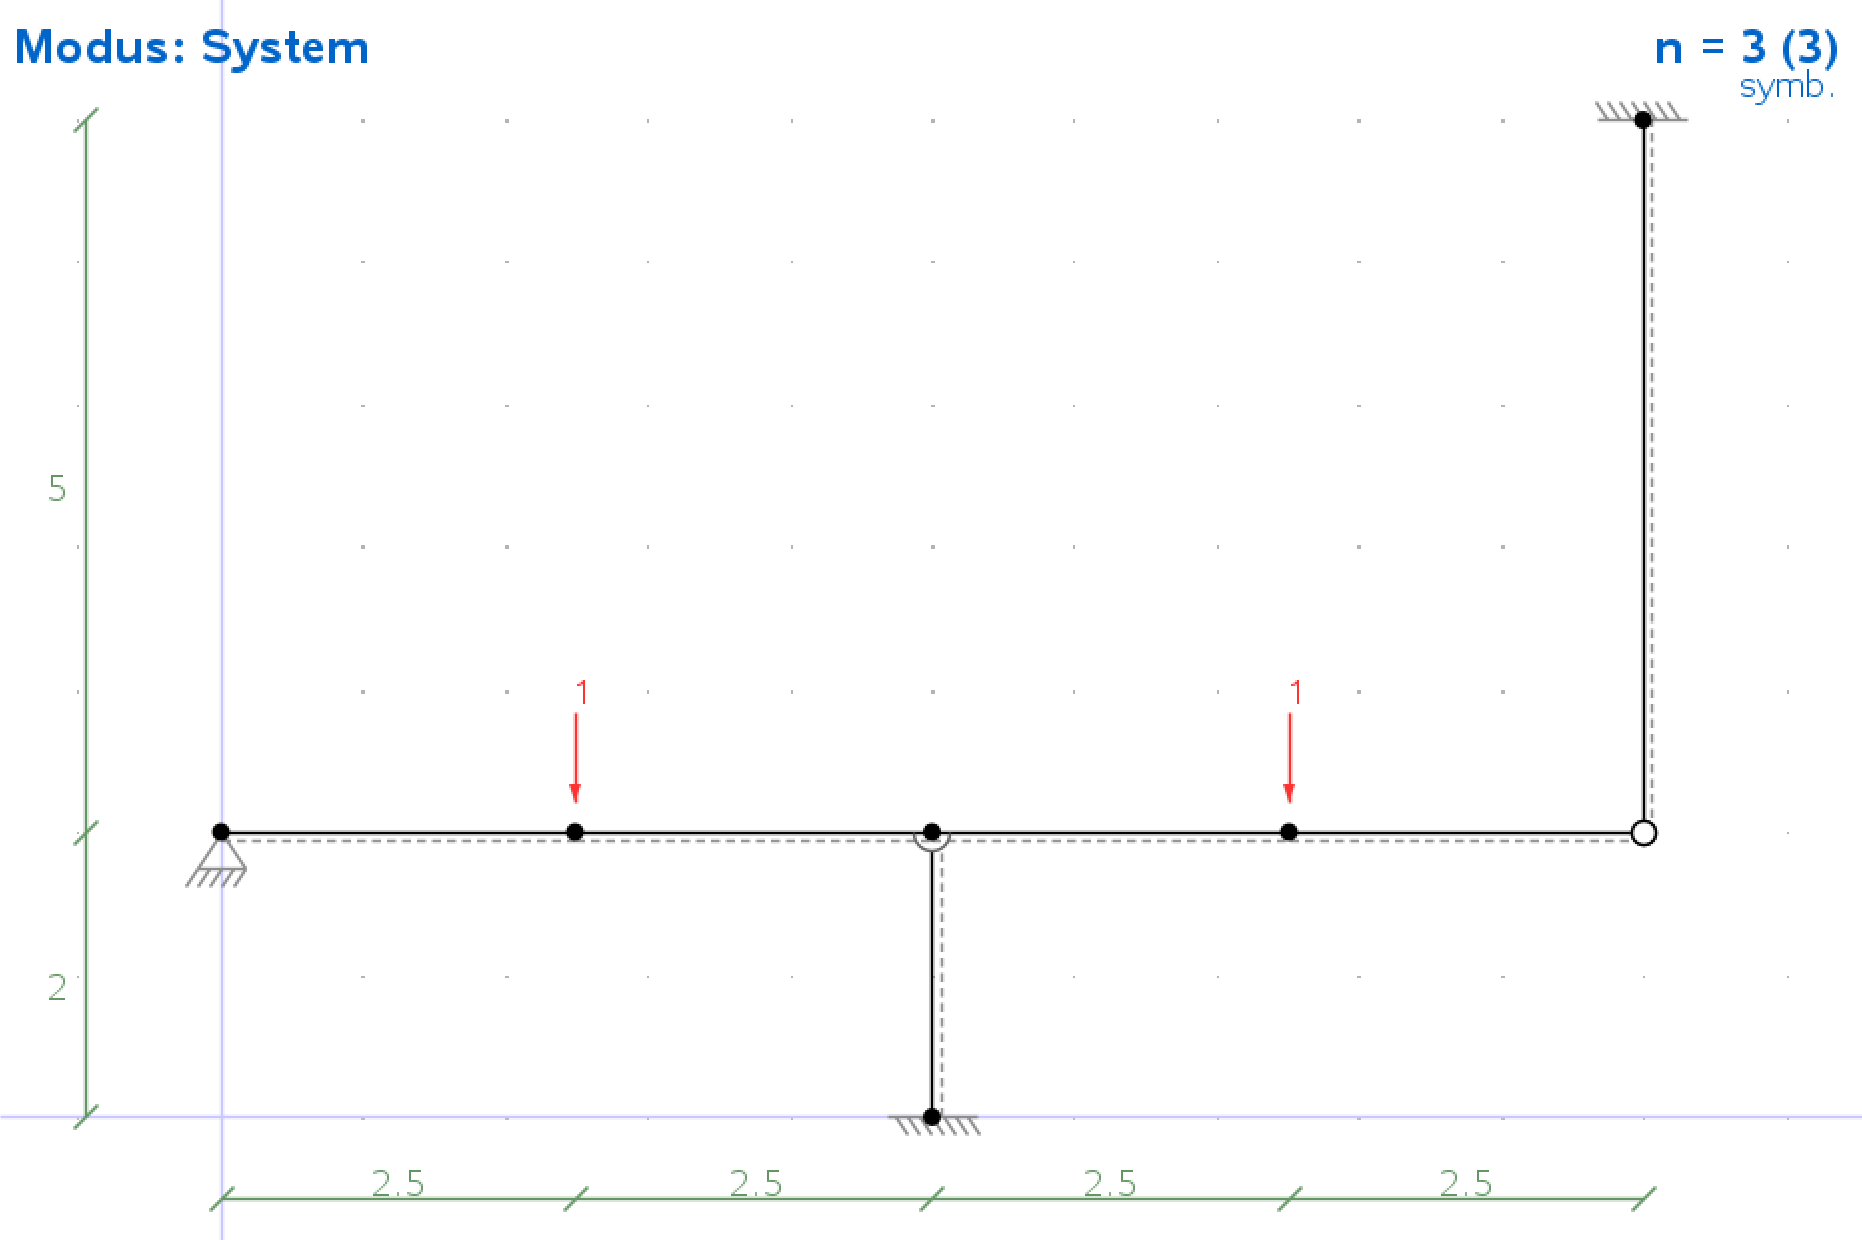
\includegraphics[width=0.5\linewidth]{./fig/TM2/WiSe2021nr4_1.png}
    \caption{TM2 WiSe~20/21, Nr.~4a im Programm}
    \label{fig:verschiebungSystem}
\end{figure}

In den \emph{neuen} Exportfunktionen wird die Temperatur auch symbolisch miteinberechnet.
Um also ann die Verschiebung des rechten unteren Knoten zu kommen lässt sich das entweder über die obere
Knotenexportfunktion machen, über die Biegelinie des rechten horizontalen Stabes oder über die Längsverschiebungsfunktion
des rechten vertikalen Stabes. Über den CAS Befehl \code{solve()} lässt sich die Temperatur direkt ausrechnen 
(vgl. Abb.~\ref{fig:verschiebungErgebniss}). Ich habe hier die Tempertur $dt$ genant (nur $T$ ist wie bereits erwähnt nicht erlaubt),
die Variable nach der aufgelöst werden soll muss der \code{solve()} Funktion als zweites Argument mit gegeben werden.

\begin{figure}[htbp]
    \centering
    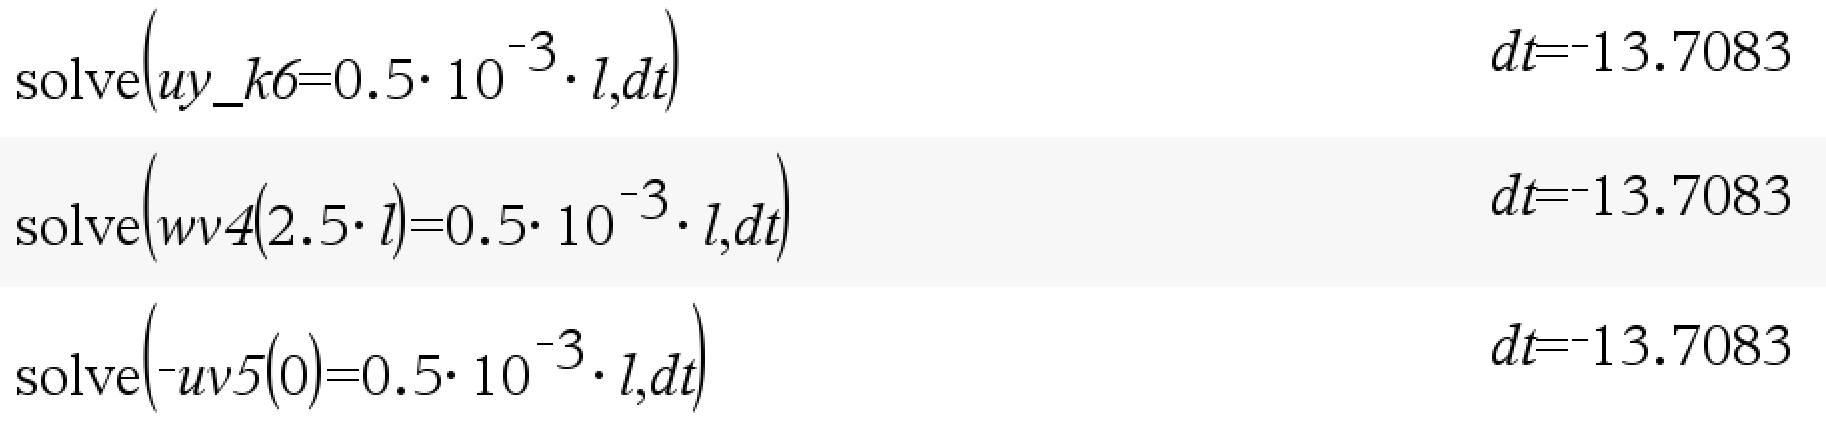
\includegraphics[width=0.5\linewidth]{./fig/TM2/WiSe2021nr4_2.png}
    \caption{Lösung von TM2 WiSe~20/21, Nr.~4a}
    \label{fig:verschiebungErgebniss}
\end{figure}

Der Zweite Teil der Aufgabe lässt sich auch im Programm lösen (Abb.~\ref{fig:VerschiebungTemp}), jedoch gibt es auch hier
ein paar Feinheiten. Ein deratiges System zu speichern kann sich lohnen. Auch hier gelten natürlich die gleichen Hinweise zu den Einheiten.

\begin{figure}[htbp]
    \centering
    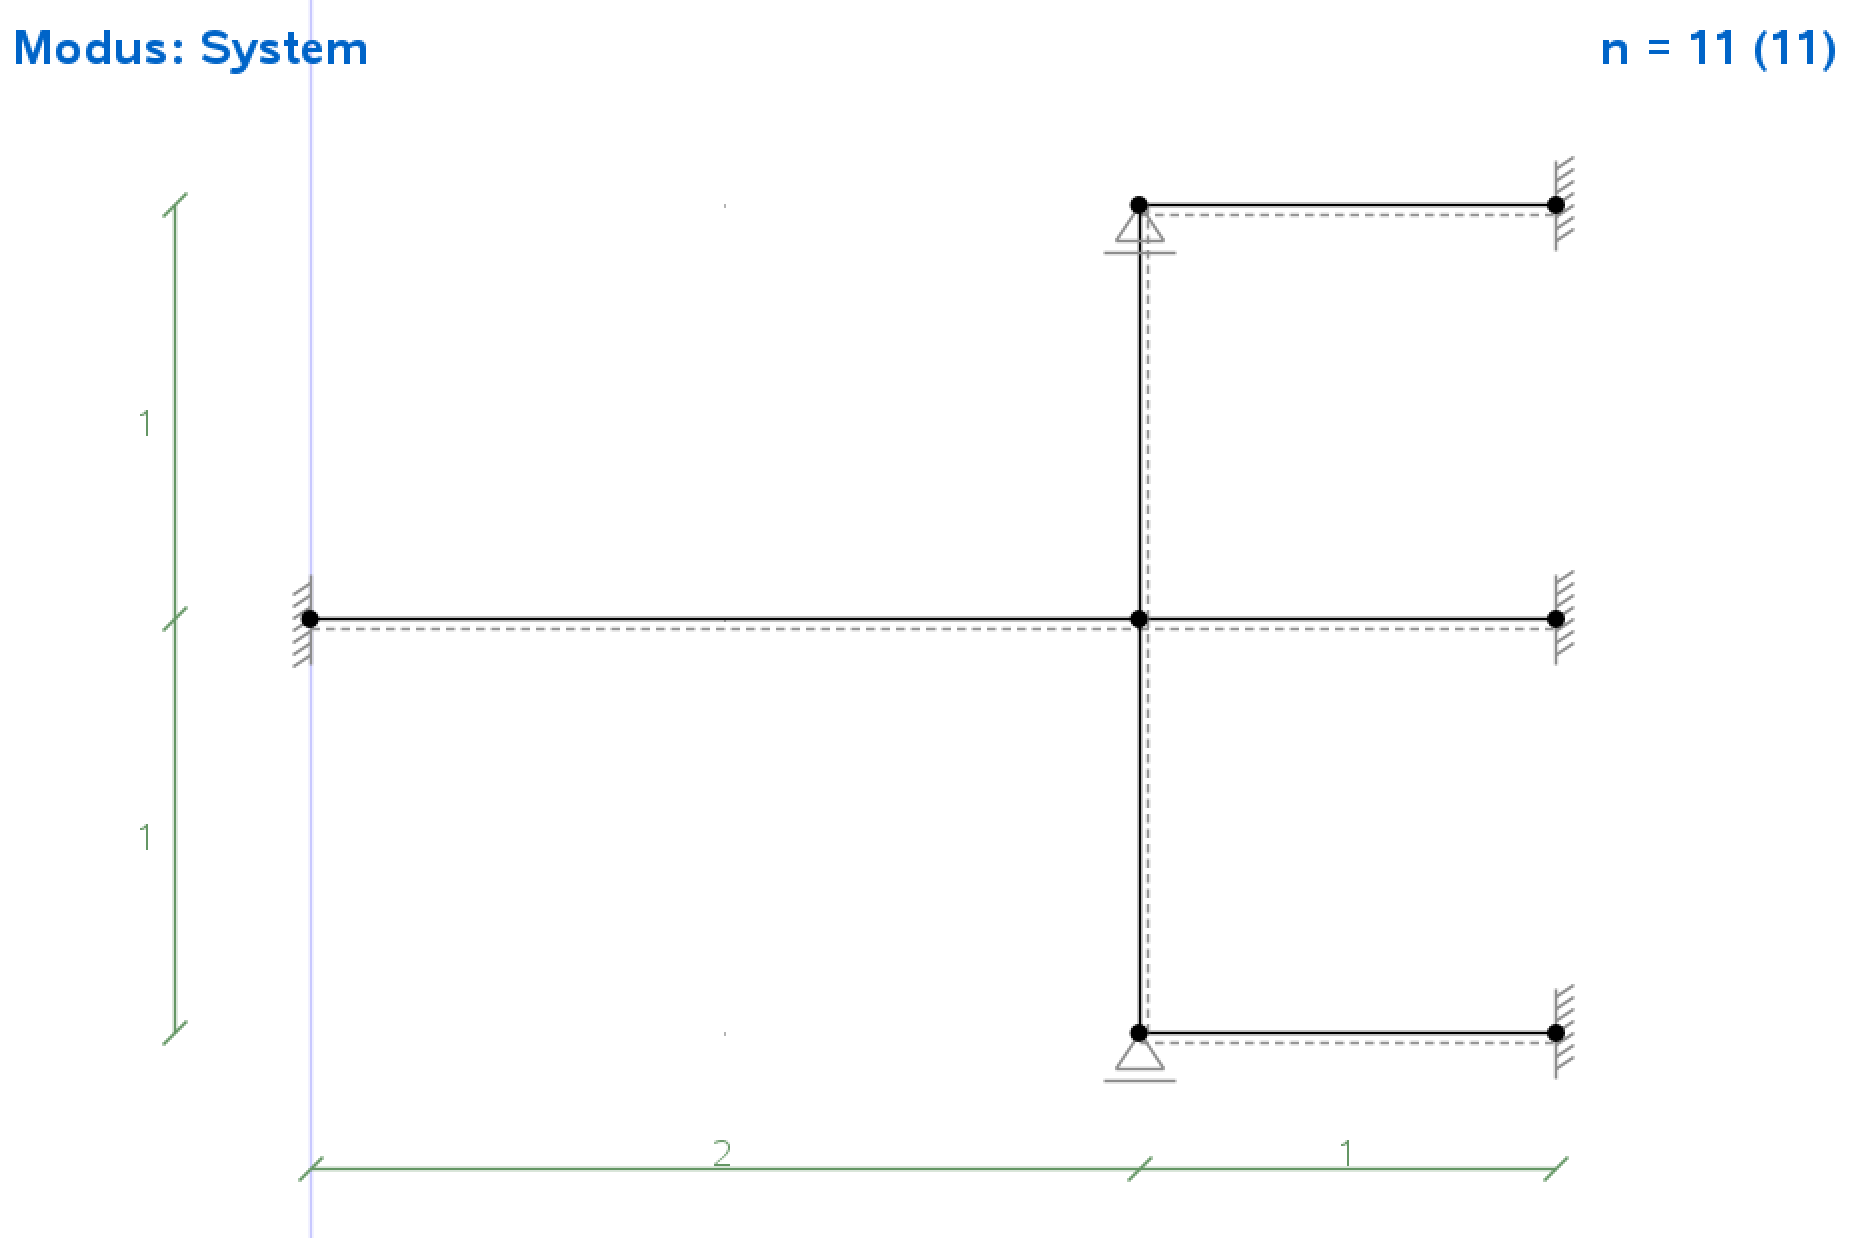
\includegraphics[width=0.5\linewidth]{./fig/TM2/WiSe2021nr4_3.png}
    \caption{TM2 WiSe~20/21, Nr.~4b im Programm}
    \label{fig:VerschiebungTemp}
\end{figure}

Da das Programm nur schnittgrößen direkt berechnet müssen diese noch in Spannungen umgerechnet werden, dafür gibt es in diesem Fall
zwei Möglichkeiten (vgl. Abb.\ref{fig:TM2WiSe2021Nr4b}). Entweder man rechnet die Spannunge direkt über die Schnittkraftverläufe aus,
oder über die Ableitung der Verschiebungsfunktion. Für die zweite Methode muss jedoch darauf geachtet werden den Temperatur Anteil
korrekt zu verrechnen.\\
Erstere Methode ist für Aufgaben mit Zahlenwerten auf jeden Fall die Einfachere, für Aufgaben mit symbolischen Temperatur Werten muss jedoch
die zweite Methode gewählt werden, da die Schnittkraftverläufe diese nicht auf die gewünschte Art berücksichtigen.

\begin{figure}[htbp]
    \centering
    \begin{subfigure}[t]{0.48\textwidth}
        \centering
        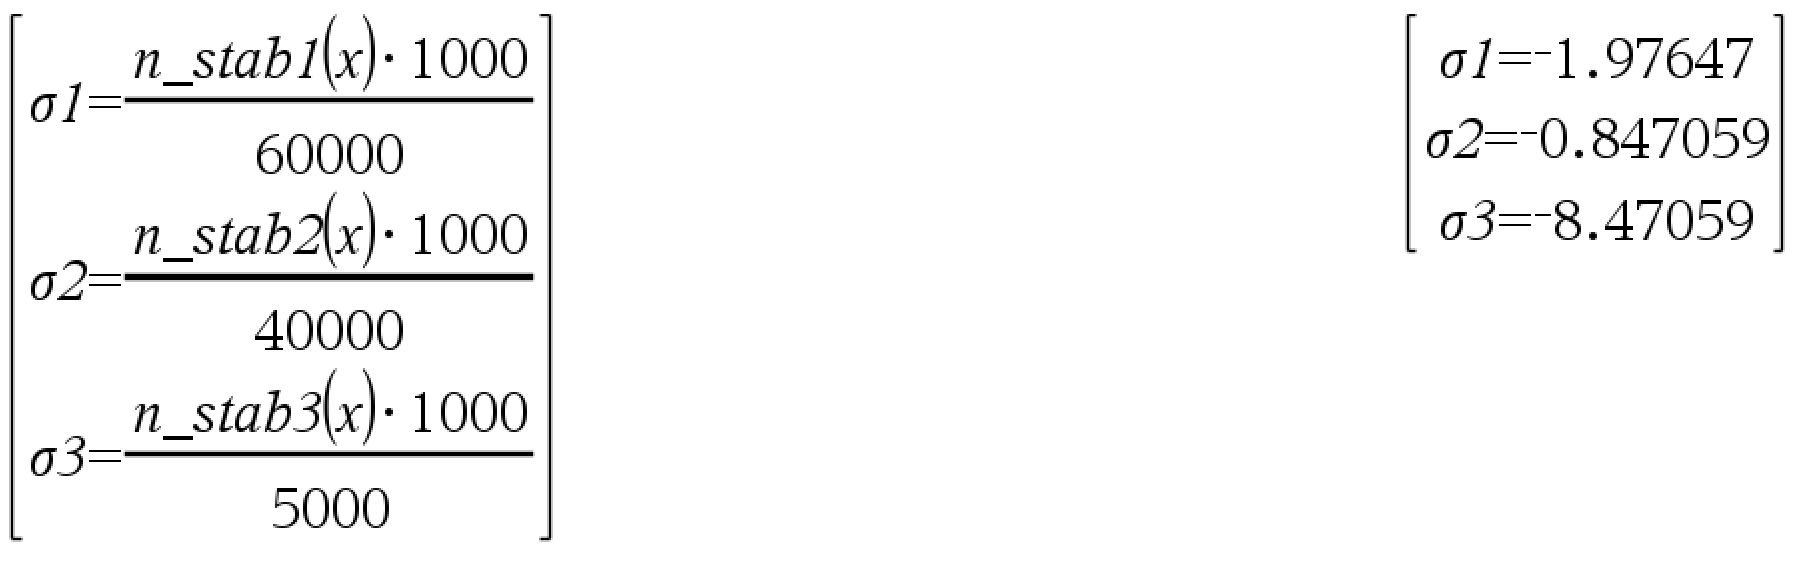
\includegraphics[width=\linewidth]{./fig/TM2/WiSe2021nr4_4.png}
        \caption{Über Schnittgrößen}
    \end{subfigure}
    \hfill
    \begin{subfigure}[t]{0.48\textwidth}
        \centering
        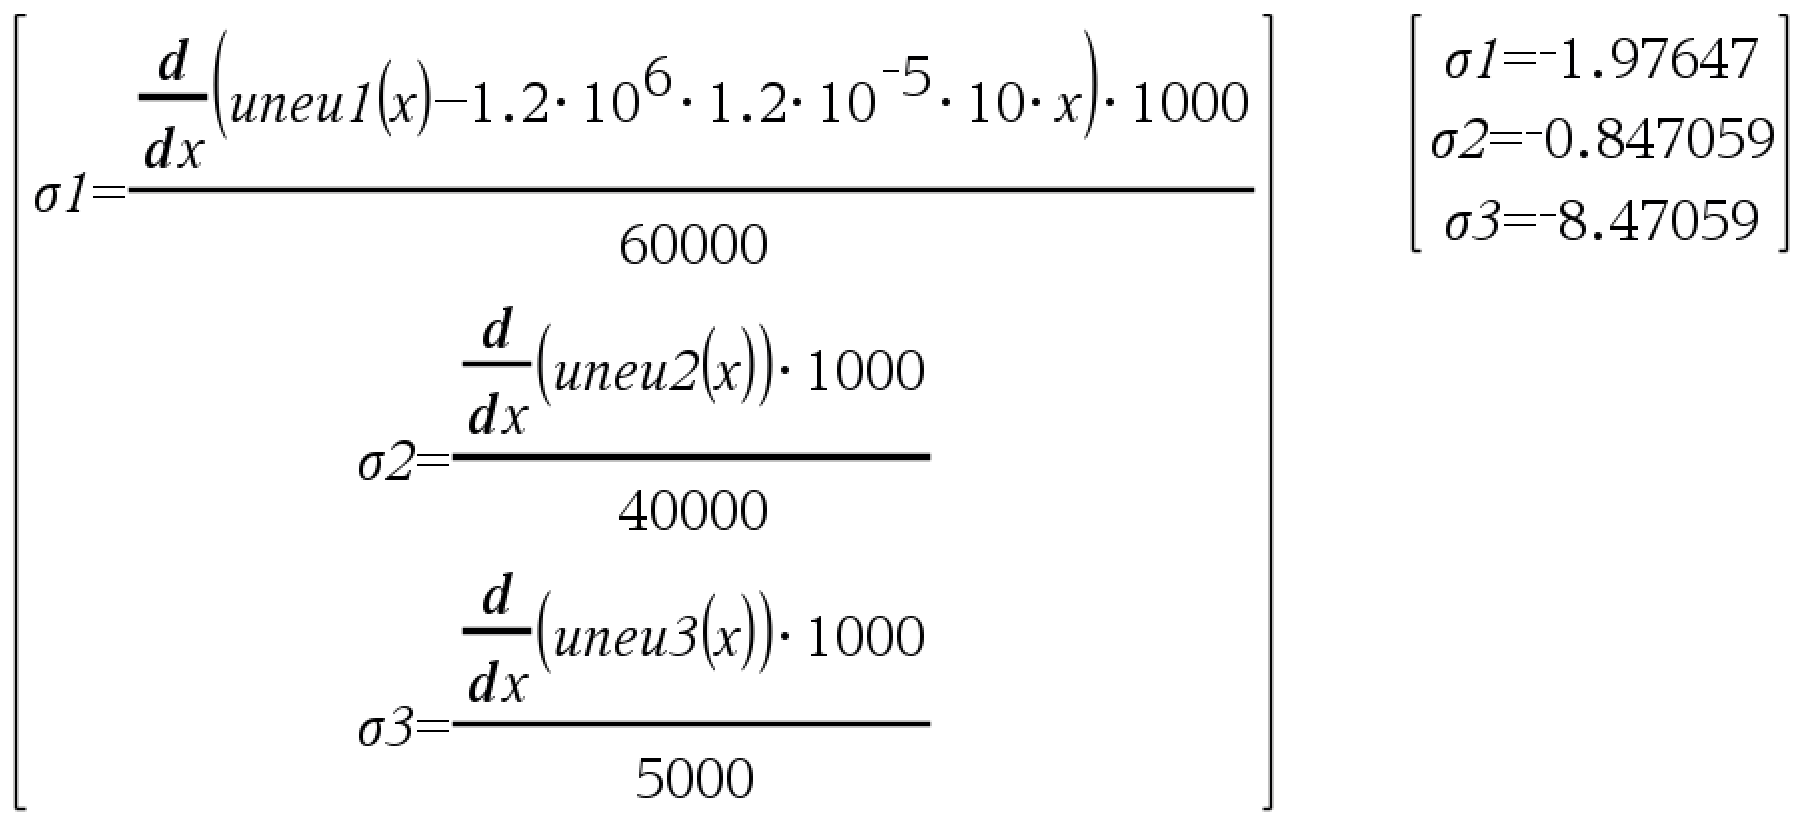
\includegraphics[width=\linewidth]{./fig/TM2/WiSe2021nr4_5.png}
        \caption{Über Verschiebungsfunktion}
    \end{subfigure}
    \caption{Lösung von TM2 WiSe~20/21, Nr.~4b}
    \label{fig:TM2WiSe2021Nr4b}
\end{figure}

Ich will hier anmerken das bei dieser Aufgabenart häufig Hinweise und Warnungen angezeigt werden. Wie z.B. hier auch bei Teilaufgabe a) eine Warnung
zur symbolischen Temperatur. Diese Warnungen sind zwar so konzipiert, dass sie nur angezeigt werden wenn das Programm bzw. ich denke
das etwas falsch eingegeben wurde, jedoch ist es schwer dabei zu vermeiden das auch bei richtiger Eingabe nie eine Warnung oder Hinweis kommt.
Aus diesem Grund empfehele ich, wenn nicht direkt ersichlich ist warum eine Warnung kommt die komplette Eingabe nochmal zu prüfen,
falls diese aber wirklicht korrekt ist sollten auch die Ergebnisse stimmen.


\subsection{Pendelstabannahme (TM2 WiSe 22/23 Nr.~4)} \label{ex:Pendelstabannahme}

\begin{figure}[htbp]
    \centering
    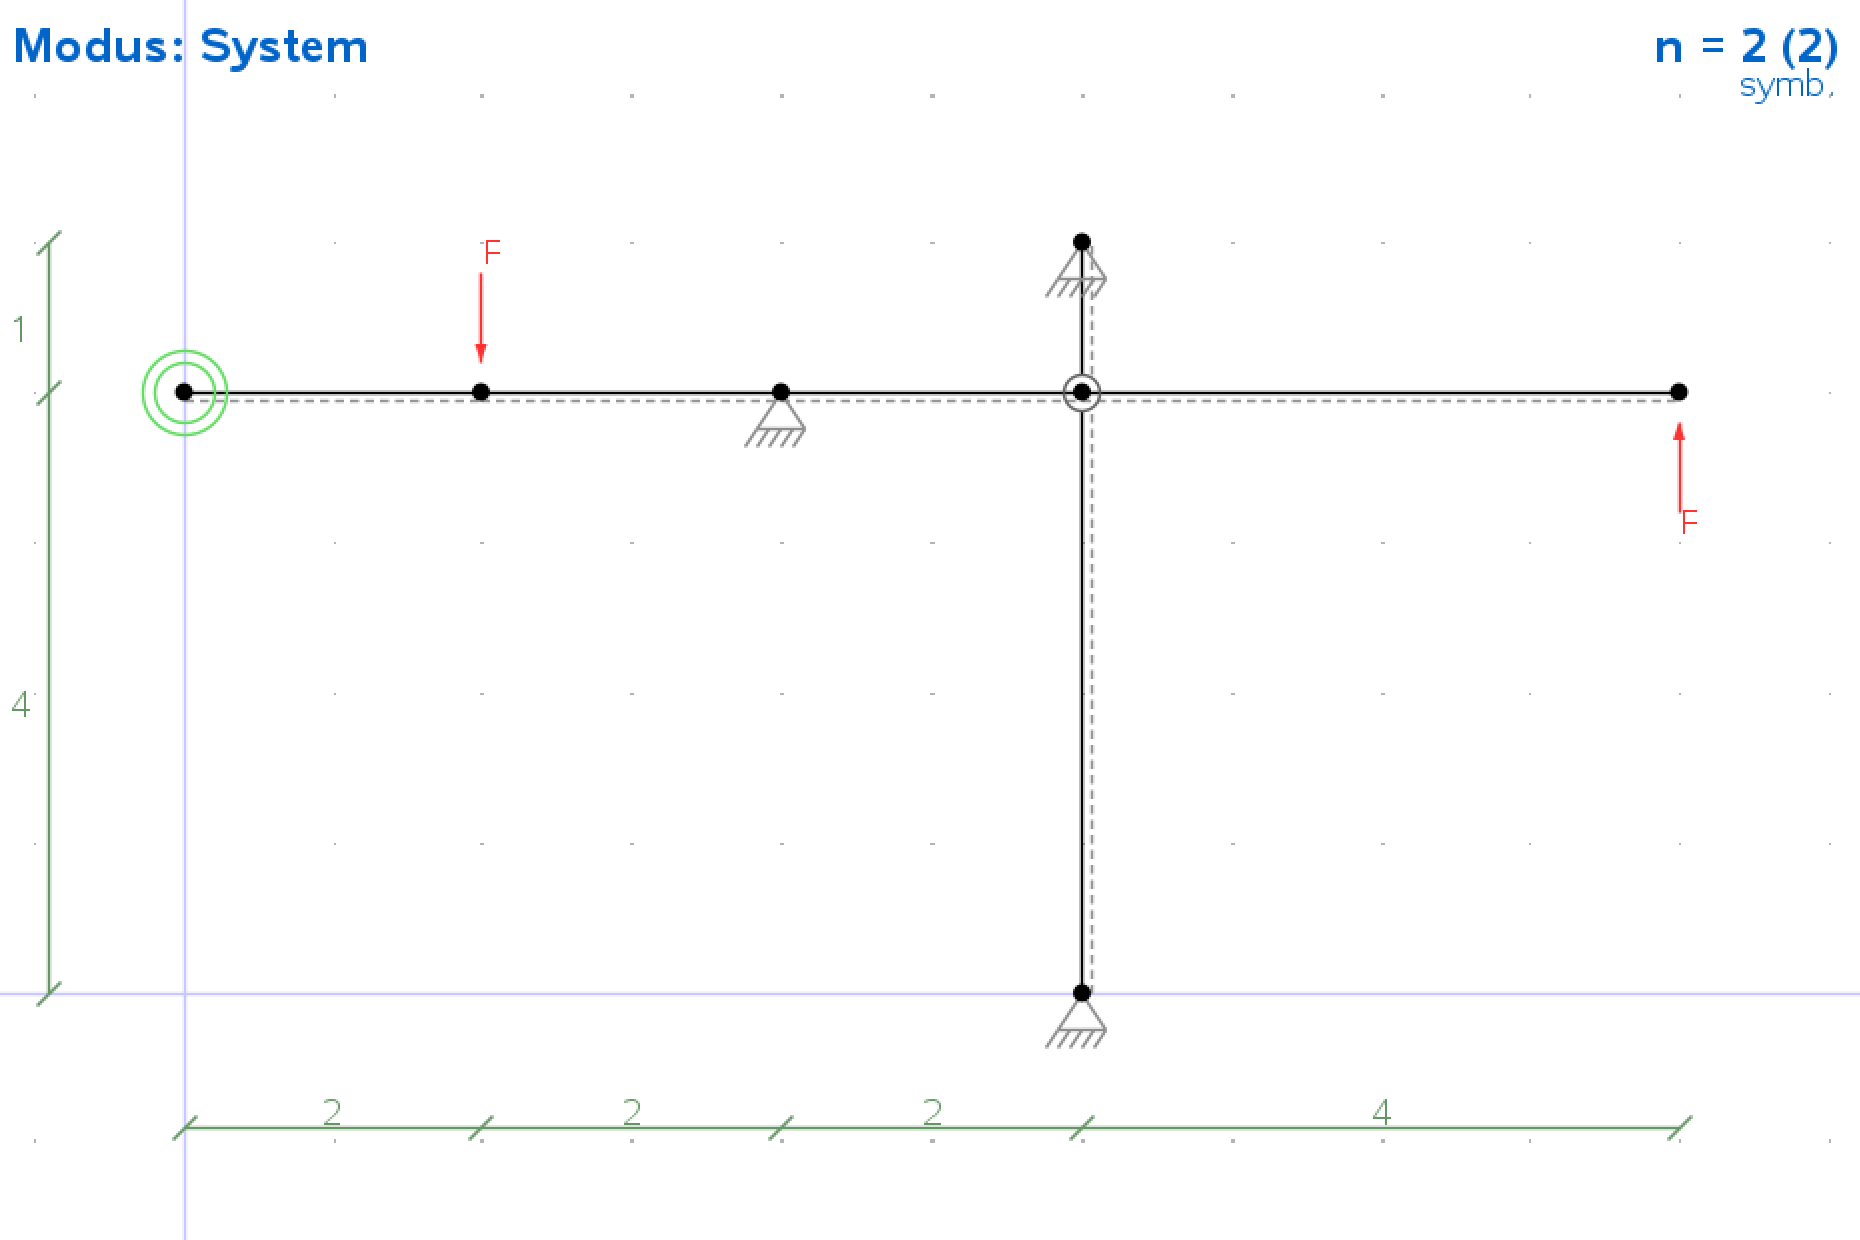
\includegraphics[width=0.7\linewidth]{./fig/TM2/WiSe2223nr4_1.png}
    \caption{TM2 WiSe~22/23, Nr.~4 im Programm}
    \label{fig:Pendelstabsnnahme}
\end{figure}

Wie die Überschrifft vielleicht bereits vermuten lässt muss bei dieser Aufgabe eine Annahme getroffen werden,
die der Zeichnung strenggenommen wiederspricht. Die beiden vertikalen stäbe sollten eigentlich mit einem Angelenk
an den starren Stab angeschlossen werden.\\
Bei einer Handrechnung wird diese Annahme quasi automatisch getroffen, das Programm macht sowas natürlich nicht automatisch.
Um diese Aufgabe mit dem Programm also korrekt zu rechnen müsseb bei den beiden vertikalen stäbe jeweils Angelenke eingebaut werden.
Falls man das nicht macht wirft das Programm eine Warnung bzw. einen Hinweis.

Bei dieser Aufgabe lassen sich die Ergebnisse entweder aus der Ansicht zur Normalkraft 
oder aus dem E-Modus holen (Abb.~\ref{fig:TM2WiSe2223Nr4}).

\begin{figure}[htbp]
    \centering
    \begin{subfigure}[t]{0.48\textwidth}
        \centering
        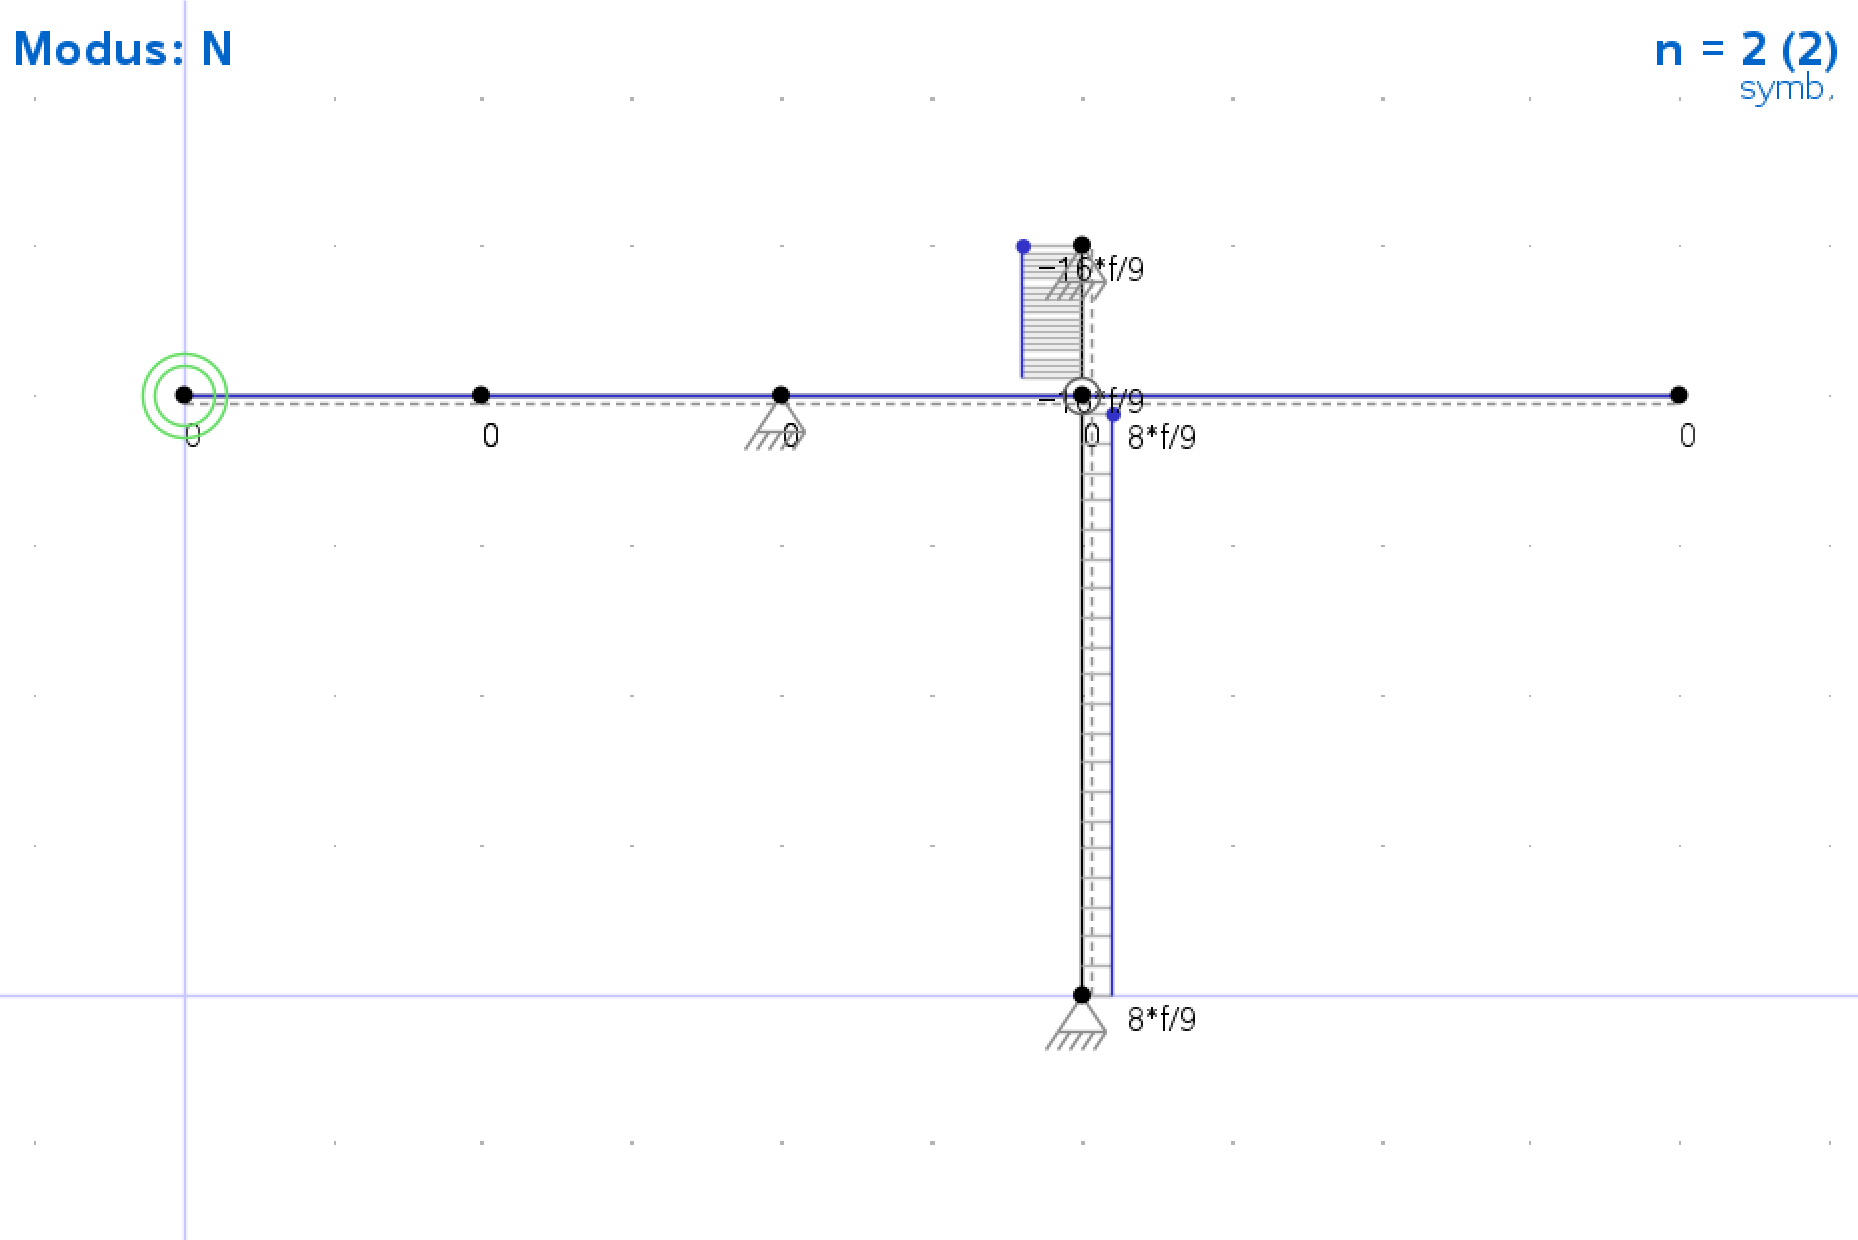
\includegraphics[width=\linewidth]{./fig/TM2/WiSe2223nr4_2.png}
        \caption{Normalkraft}
    \end{subfigure}
    \hfill
    \begin{subfigure}[t]{0.48\textwidth}
        \centering
        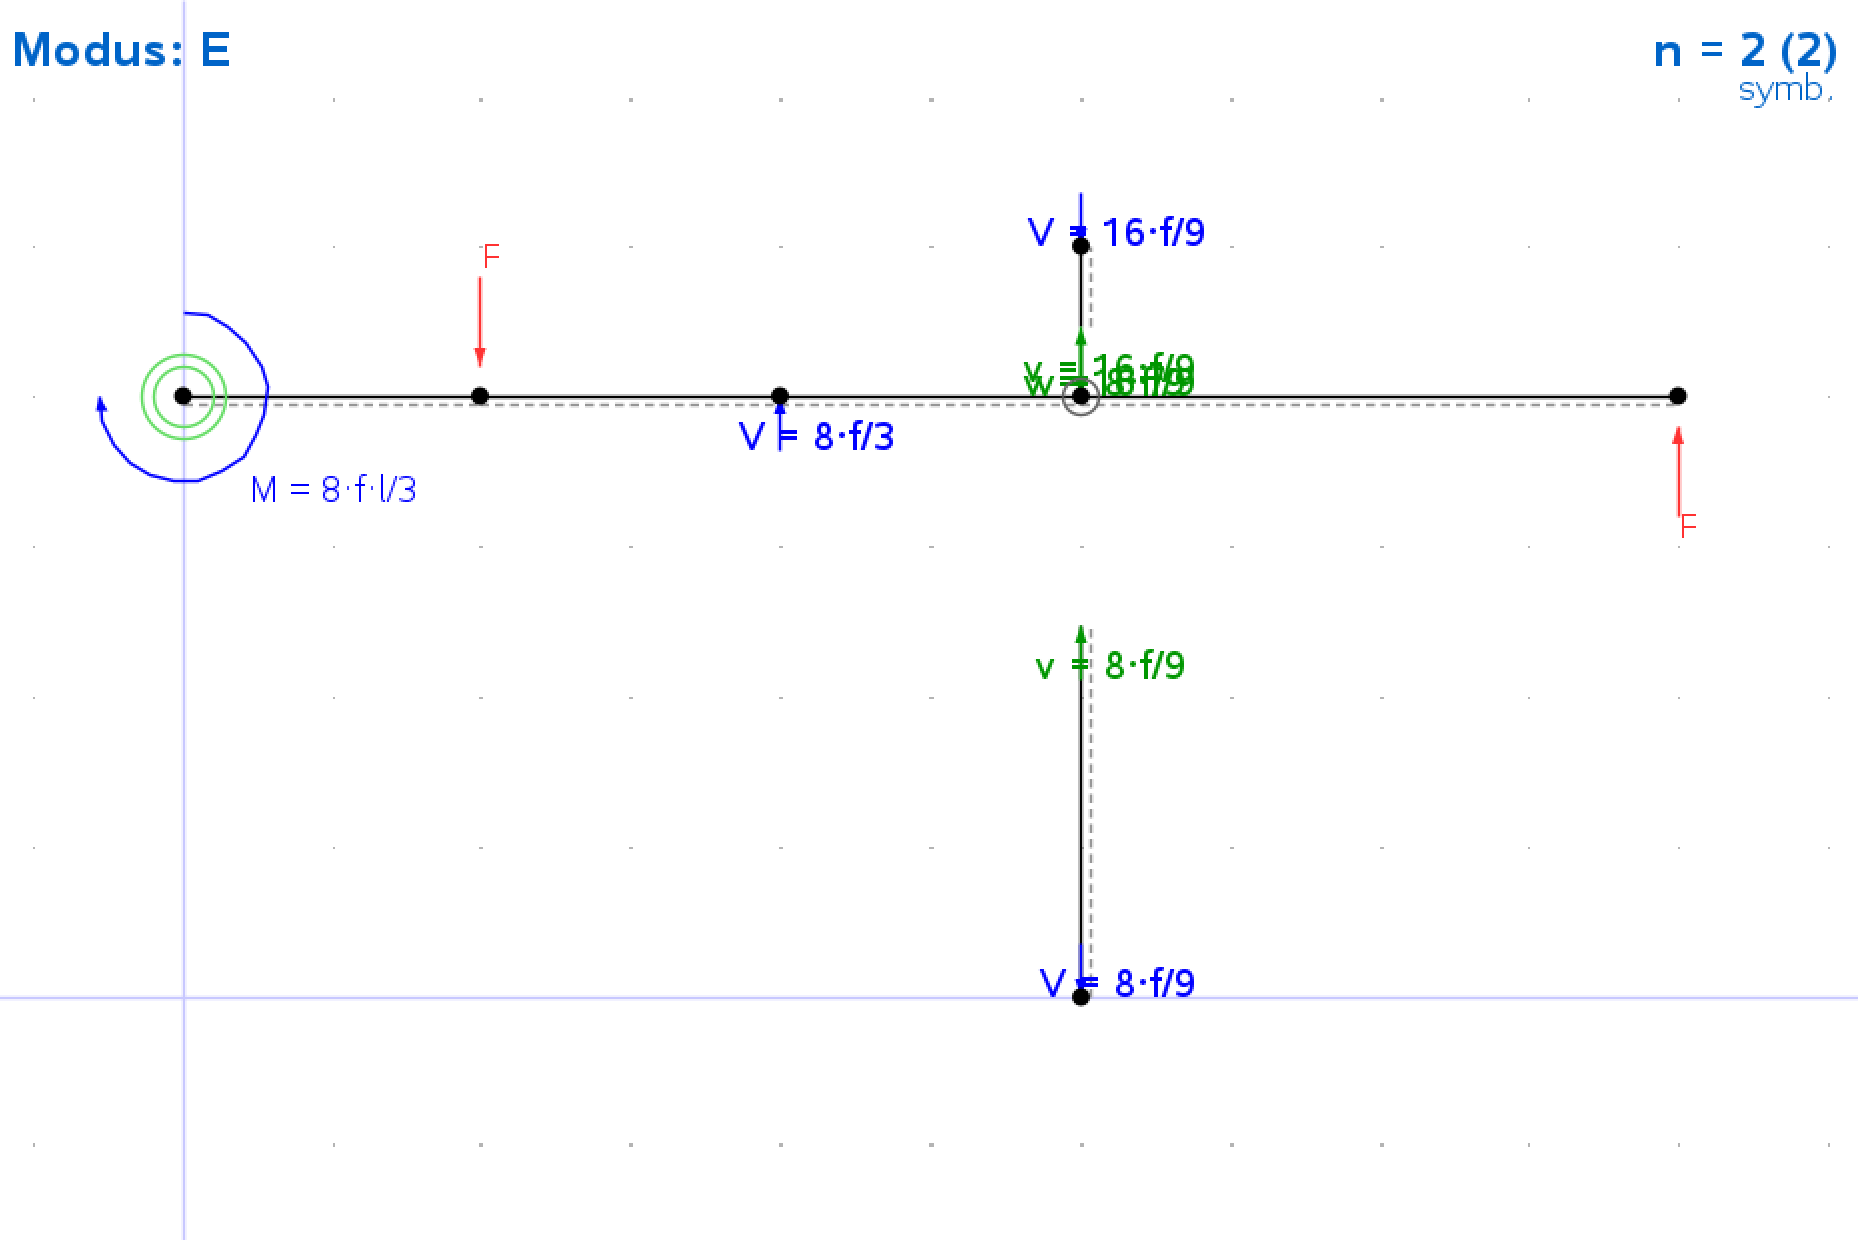
\includegraphics[width=\linewidth]{./fig/TM2/WiSe2223nr4_3.png}
        \caption{E-Modus}
    \end{subfigure}
    \caption{Lösung von TM2 WiSe~22/23, Nr.~4}
    \label{fig:TM2WiSe2223Nr4}
\end{figure}

\textbf{Wichtig} ist, dass das Programm, für symbolische Federn in den Verläufen in seltenen Fällen nicht die richtigen 
Werte ausgibt (Bei symbolischen Temperaturen sowieso nicht).
Zur Sicherheit würde ich deswegen die Schnittgrößen über die \emph{neuen} Verschiebungsfunktionen ermitteln. 
Das dauert zwar gerade für große Systeme länger, ist aber zuverlässiger weil dort wirklich alles symbolisch gerechnet wird 
und eben nicht gepfuscht wird.



\subsection{Schiefe Biegung (TM2 WiSe 25/26 Nr.~8)}

In dieser Aufgbabe sind die Dicken der dünnwandigen Elemente nicht gegeben, da diese abber sowohl für das
FTM als auch für die Lange des Schwerpunkts wichtig sind, müssen diese Werte manuell mit den Werten aus der 
Aufgabenstellung überschrieben werden. Das geht im Obermenue (Taste \taste{o}) auf Seite 3.\\
Für das Zeichnen so eines schiefen Querschnitts empfielt sich ein Rastermaß von z.B. $\frac{1}{\sqrt{2}}$.

\begin{figure}[htbp]
    \centering
    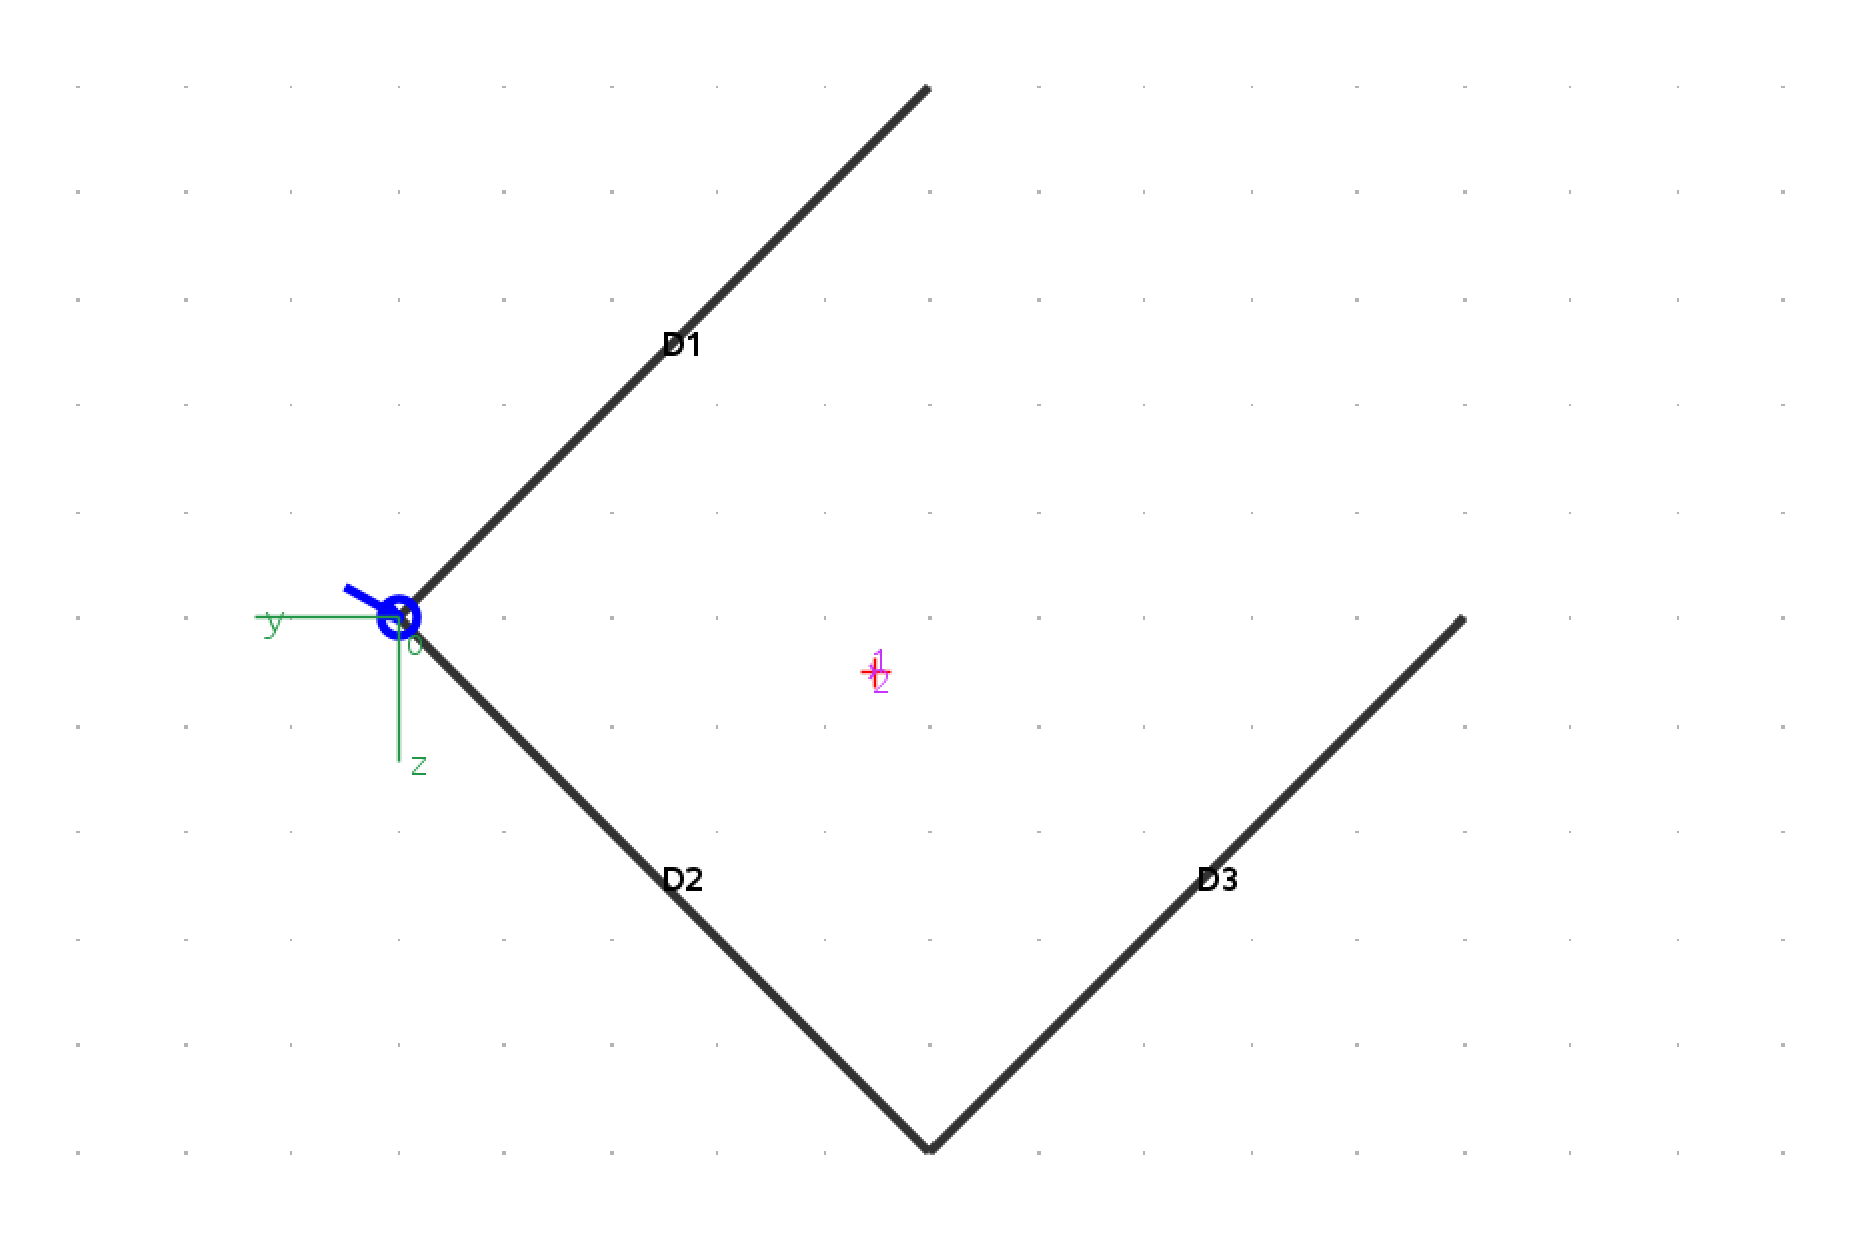
\includegraphics[width=0.7\linewidth]{./fig/TM2/WiSe2526nr8_1.png}
    \caption{TM2 WiSe~25/26, Nr.~8 im Programm}
    \label{fig:TM2WiSe2526Nr8_1}
\end{figure}

Bei dieser Aufgabe braucht man die $\sigma_x$-Berechnung. Um die Normalkraft hier richtig einzuberechnen
muss die Resultierende der Streckenlast über die halbe Länge berechnet werden, also: 
$R=0,1~\frac{\text{kN}}{cm}\cdot100~\text{cm}$.
Für die Kraft muss also $F_y=-500~\text{N}$, $F_z=300~\text{N}$ und $F_x=10000~\text{N}$ eingegeben werden.

Nach dem Aufruf der Berechnung werden noch ein paar Werte abgefragt. Für die ersten Drei muss Null eingetragen werden.
Man hätte auch keine Kraft platzieren können, die Normalkraft und Momente handisch ausrechnen können und diese dann in diese Felder eintragen können.
Das Ergebniss ist das gleiche.\\
Für $\Delta x$ muss $100~\text{cm}$ eingetragen werden, das ist der Abstand zwischen dem gezeichneten Schnitt und dem betrachteten Schnitt.
Das Programm rechnet dann also automatisch die Momente aus der Querkraft aus. Dieses Feature funktioniert natürlich nur, wenn zwischen dem gezeichneten und berechneten Schnitt
keine Weiteren Einflüsse wie Lager oder Kräfte Angreiffen, dann kommt man nicht darum herum $N$, $M_y$ und $M_z$ händisch auszurechnen und einzutragen.

Die Ergebnisse sind in Abbildung \ref{fig:TM2WiSe2526Nr8_2} dargestellt.

\begin{figure}[htbp]
    \centering
    \begin{subfigure}[t]{0.48\textwidth}
        \centering
        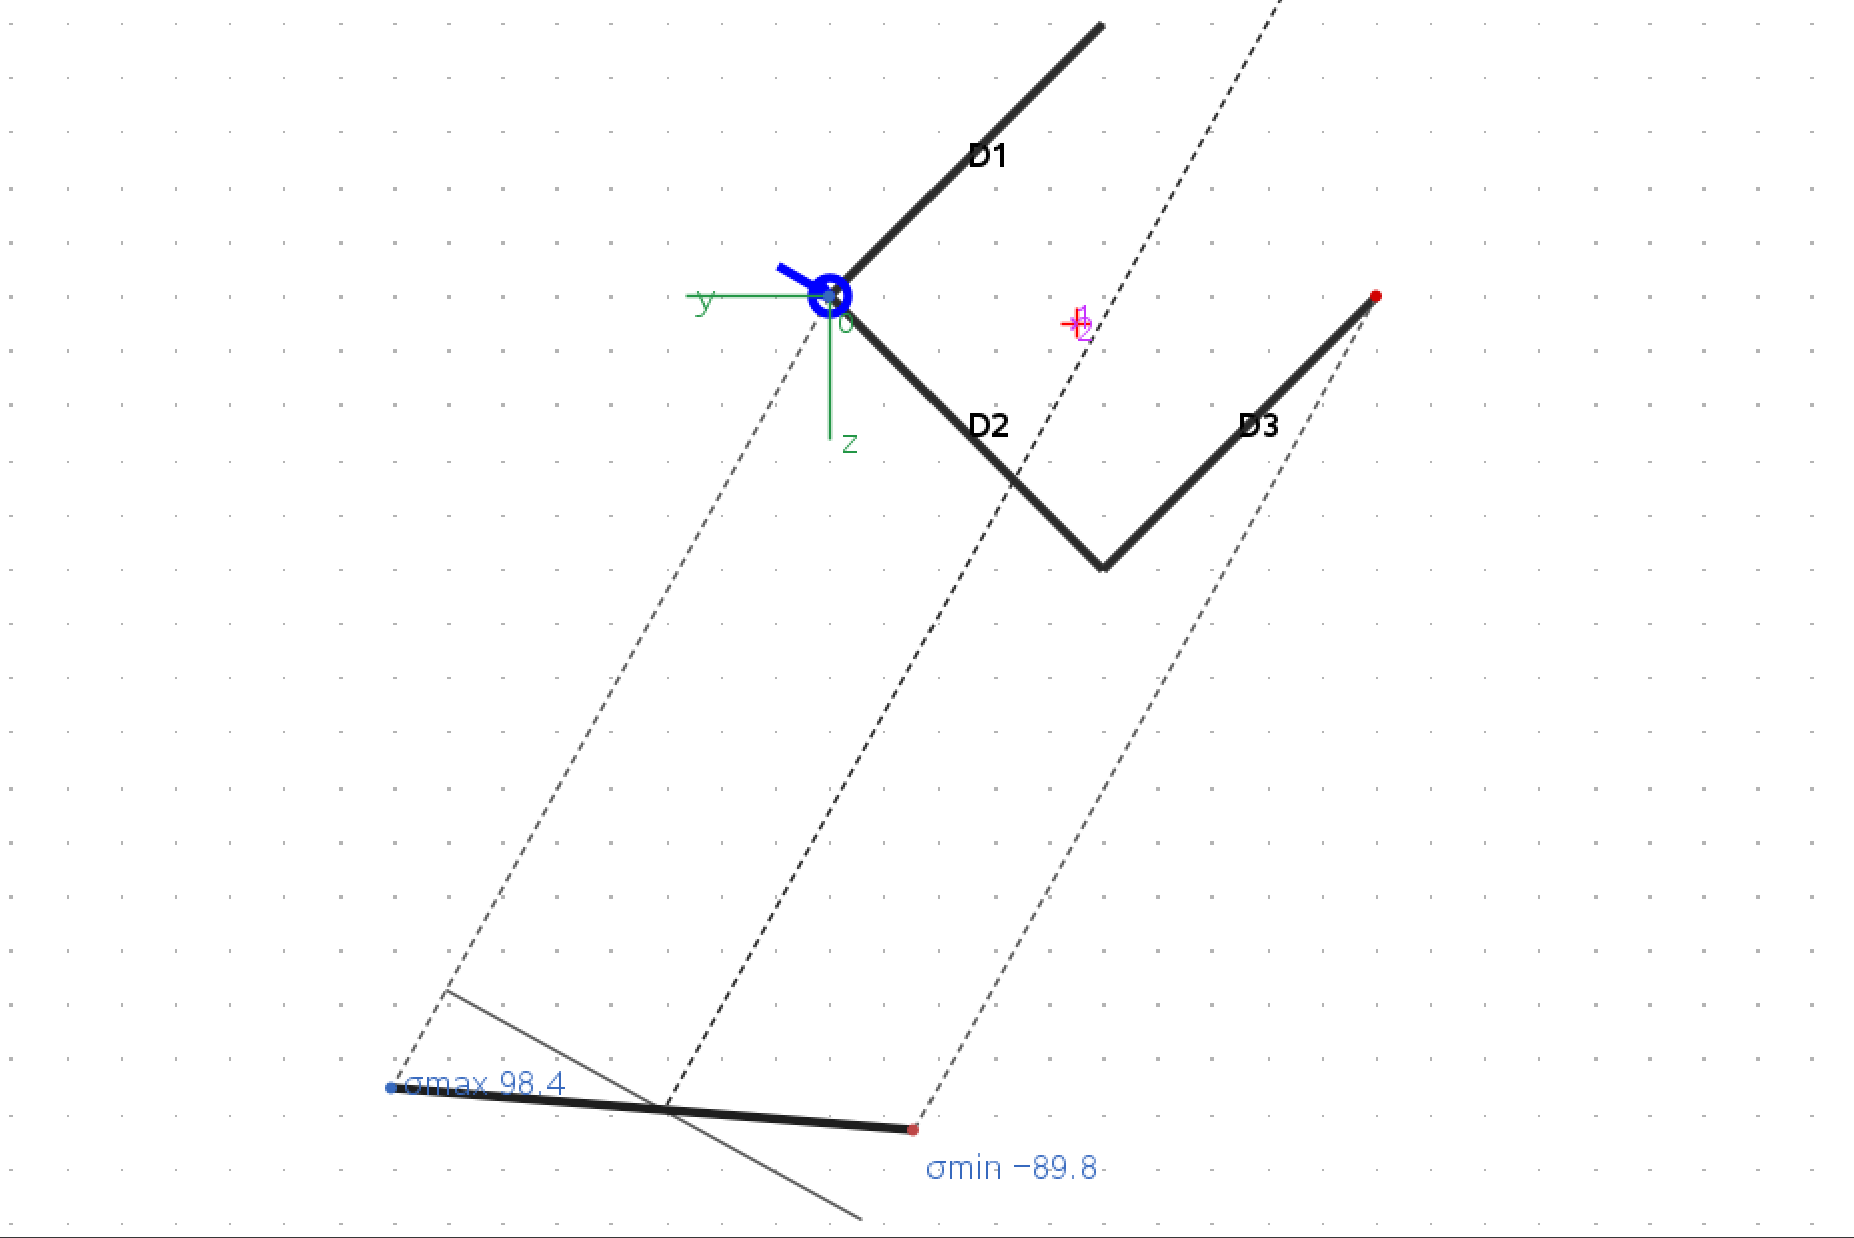
\includegraphics[width=\linewidth]{./fig/TM2/WiSe2526nr8_2.png}
        \caption{Spannungsverlauf}
    \end{subfigure}
    \hfill
    \begin{subfigure}[t]{0.48\textwidth}
        \centering
        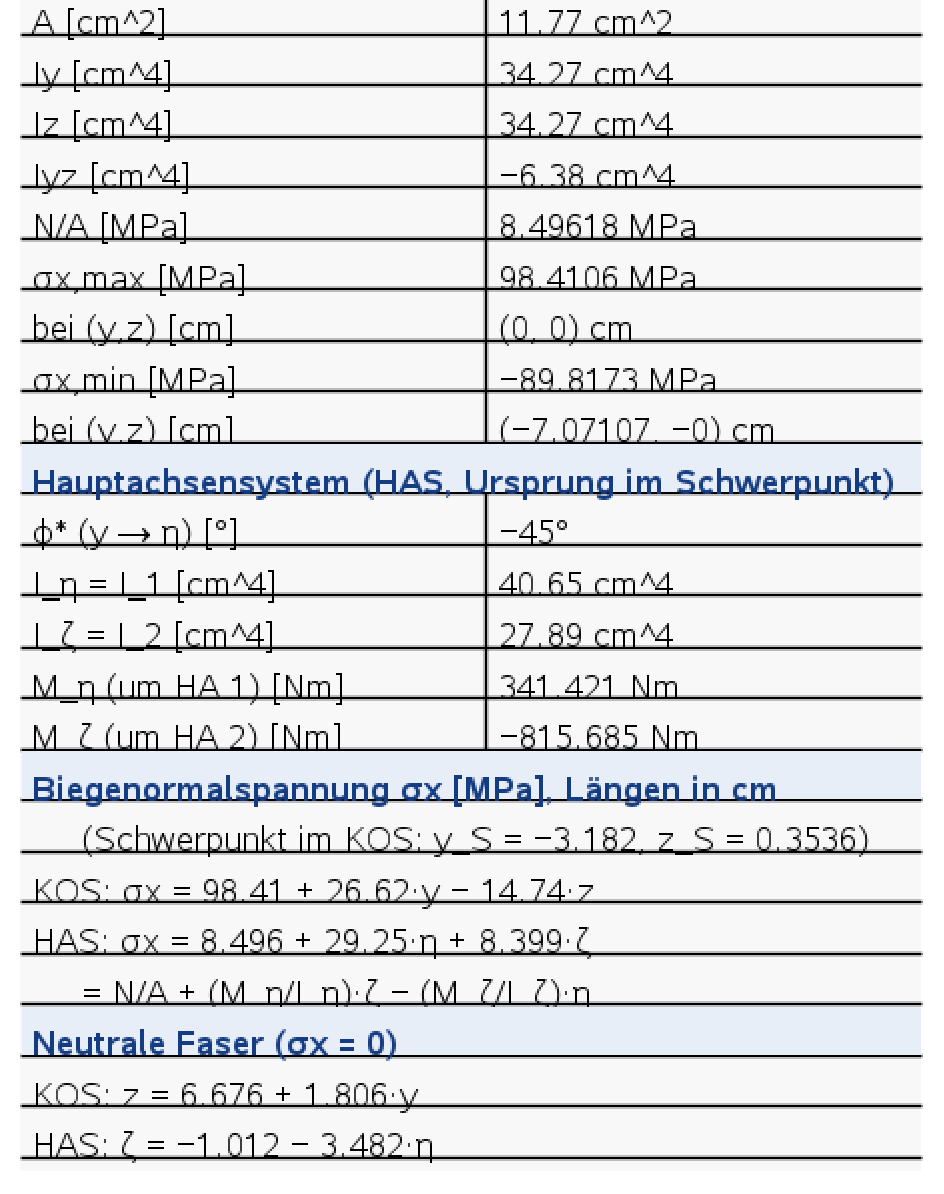
\includegraphics[width=\linewidth]{./fig/TM2/WiSe2526nr8_3.png}
        \caption{Tabellen übersicht}
    \end{subfigure}
    \caption{Lösung von TM2 WiSe~25/26, Nr.~8}
    \label{fig:TM2WiSe2526Nr8_2}
\end{figure}

Ich will anmereken, dass des öfteren bei Aufgaben Querschnittswerte gegeben sind, die nicht zur Bemaßung in der Zeichnung passen,
ob das absichtlich so ist konnte mir leider keiner sagen. Es ist also immer sinnvoll das einmal gegen zu prüfen und die Werte evtl. zu überschreiben.
Was die ISD-Musterlösung bei dieser Aufgabe gerechnet hat, ist mir nicht ganz klar. Meines Verständnisses nach wurde hier mit einem
Schwerpunkt für die Momente aus Normalkraft gerechnet, der genau in der Mitte des U profiels liegt, sodass die Normalkraft um die $y$-Achse kein Moment erzeugt.

\subsection{Schiefe Biegung/Kernfäche (TM2 WiSe21/22 Nr.~8)}



\subsection{MSK (TM2 WiSe 21/22 Nr.~3)}

Zu dieser Aufgabe gibt es eigentlich nicht besonders viel zu sagen, man gibt die gegebenen Werte ein und das Programm
füllt in grün die restlichen Werte auf (Abb.~\ref{fig:TM2WiSe2122Nr3_1}).

\begin{figure}[htbp]
    \centering
    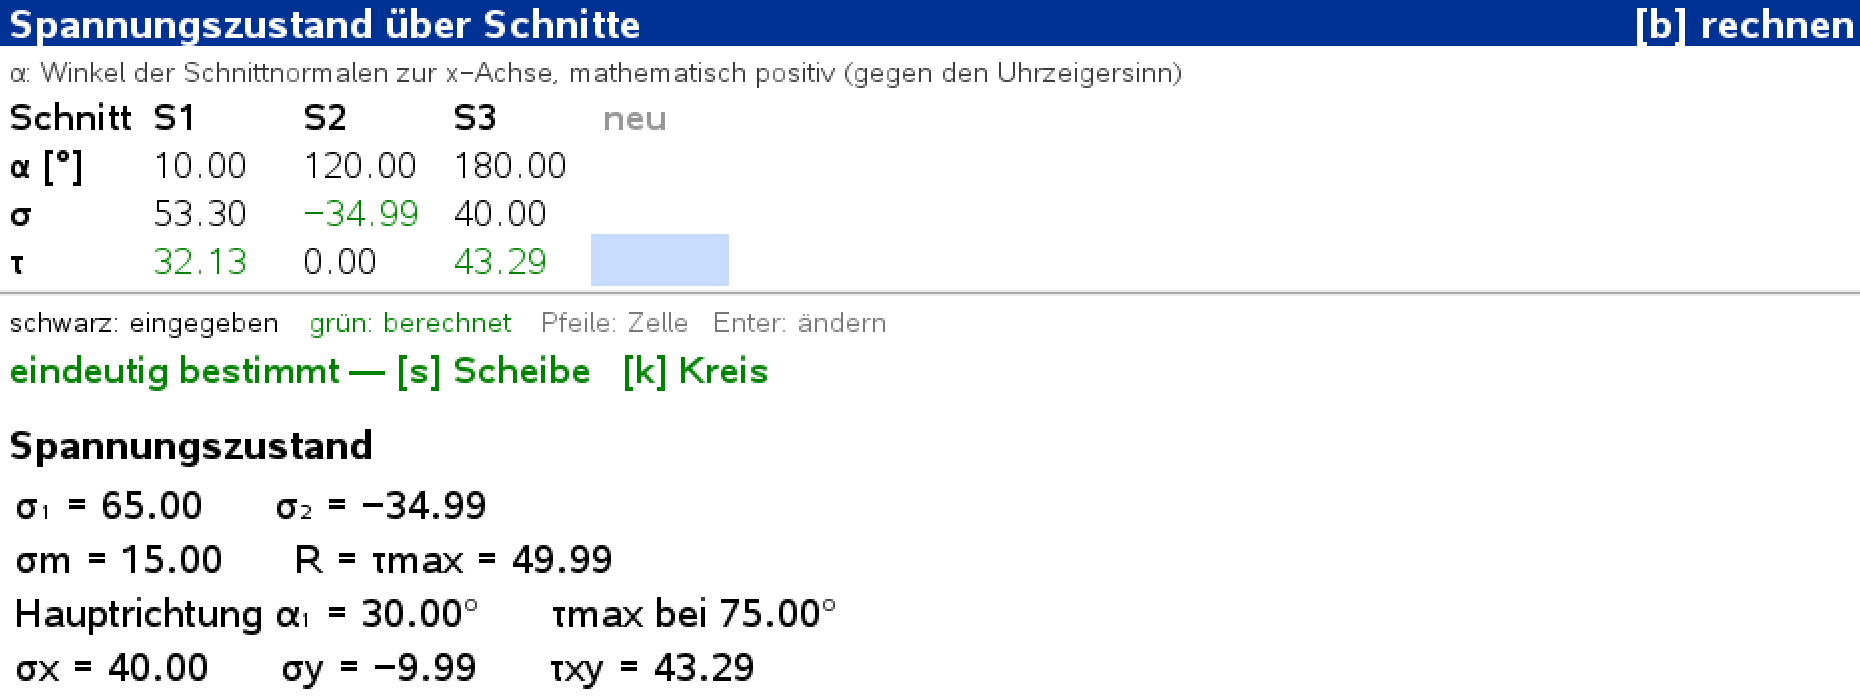
\includegraphics[width=0.7\linewidth]{./fig/TM2/WiSe2122nr3_1.png}
    \caption{TM2 WiSe~21/22, Nr.~3 im Programm}
    \label{fig:TM2WiSe2122Nr3_1}
\end{figure}

Danach bekommt man mit den Tasten \taste{s} und \taste{k} die beiden wichtigen Ansichten (Abb.~\ref{fig:TM2WiSe2122Nr3_2}).


\begin{figure}[htbp]
    \centering
    \begin{subfigure}[t]{0.48\textwidth}
        \centering
        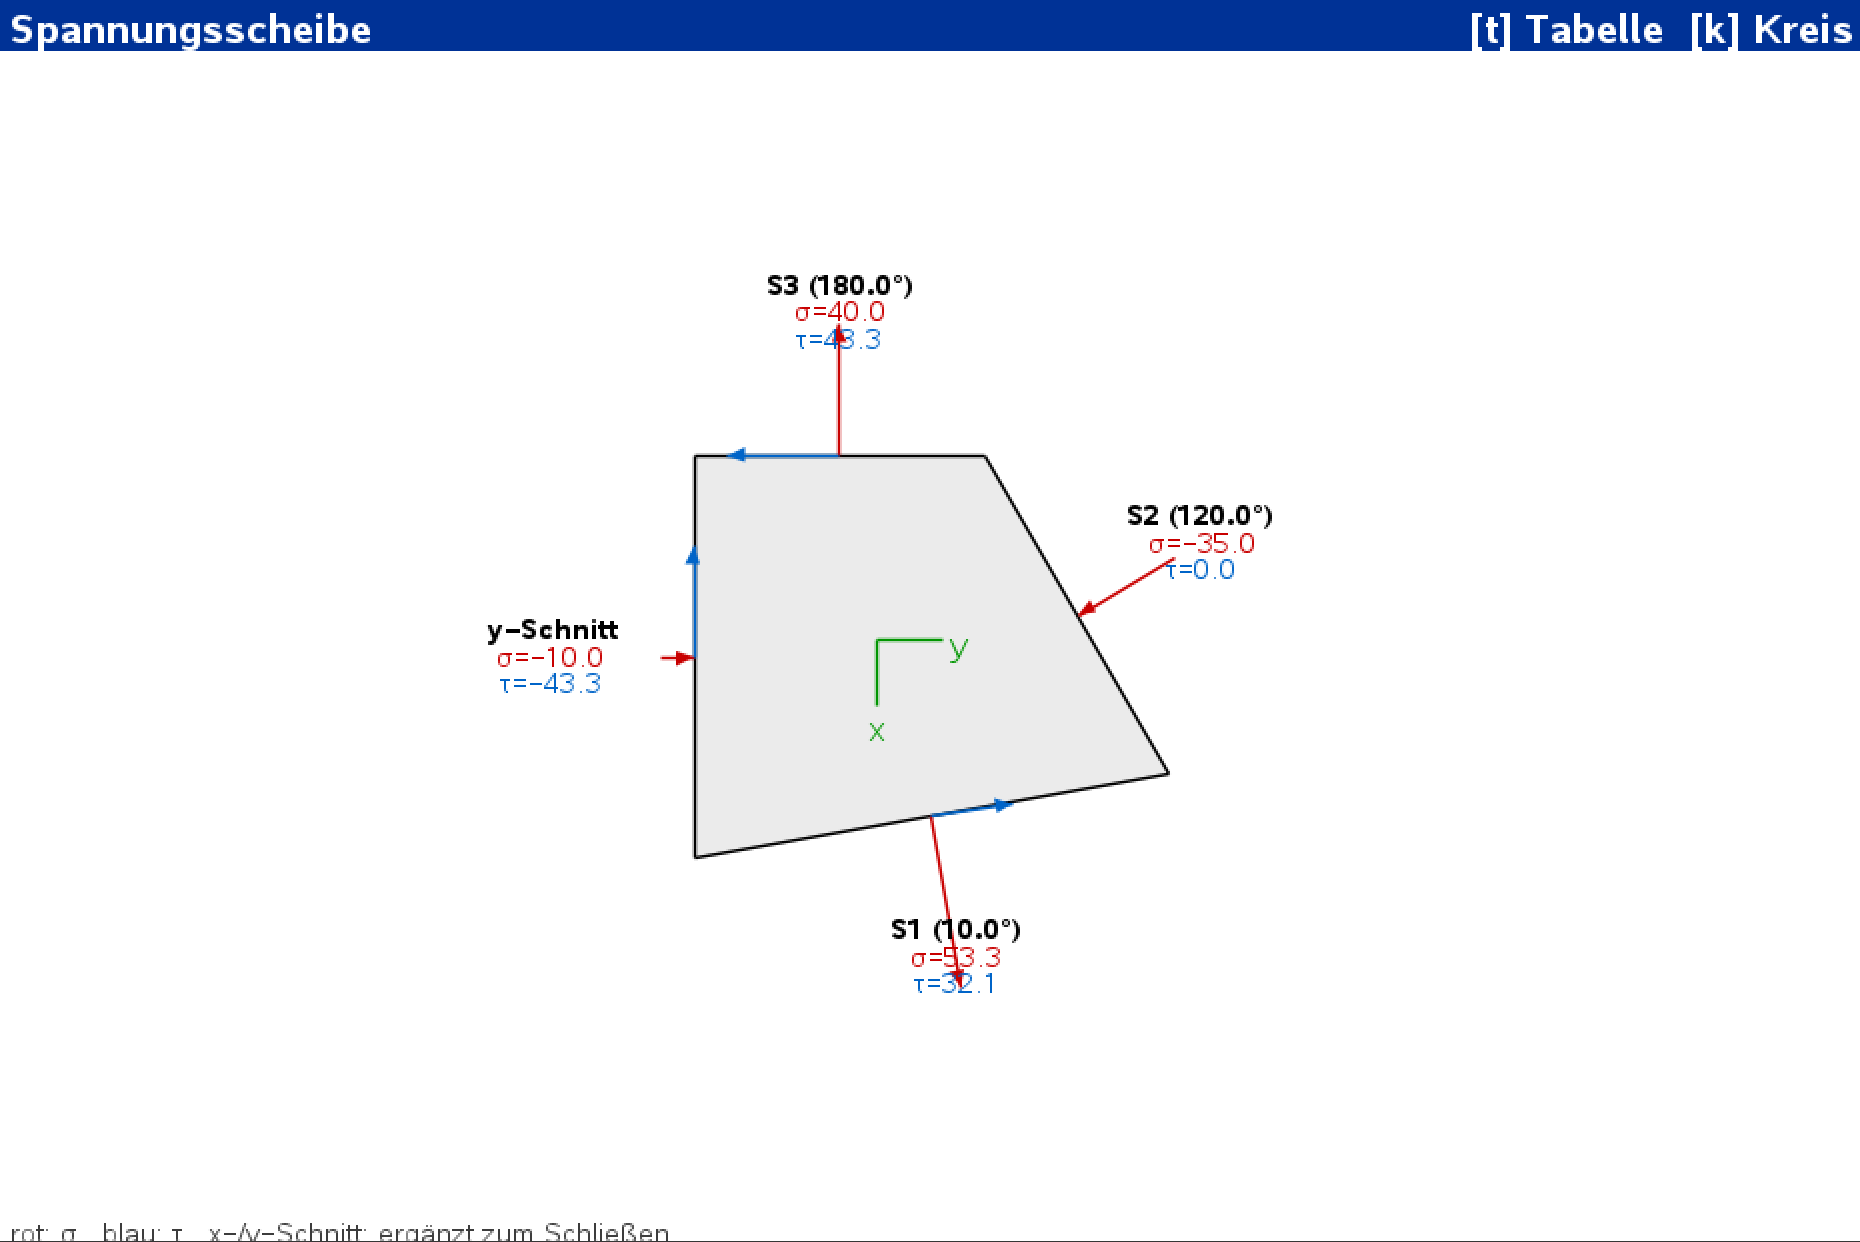
\includegraphics[width=\linewidth]{./fig/TM2/WiSe2122nr3_2.png}
        \caption{Spannungs-Scheibe}
    \end{subfigure}
    \hfill
    \begin{subfigure}[t]{0.48\textwidth}
        \centering
        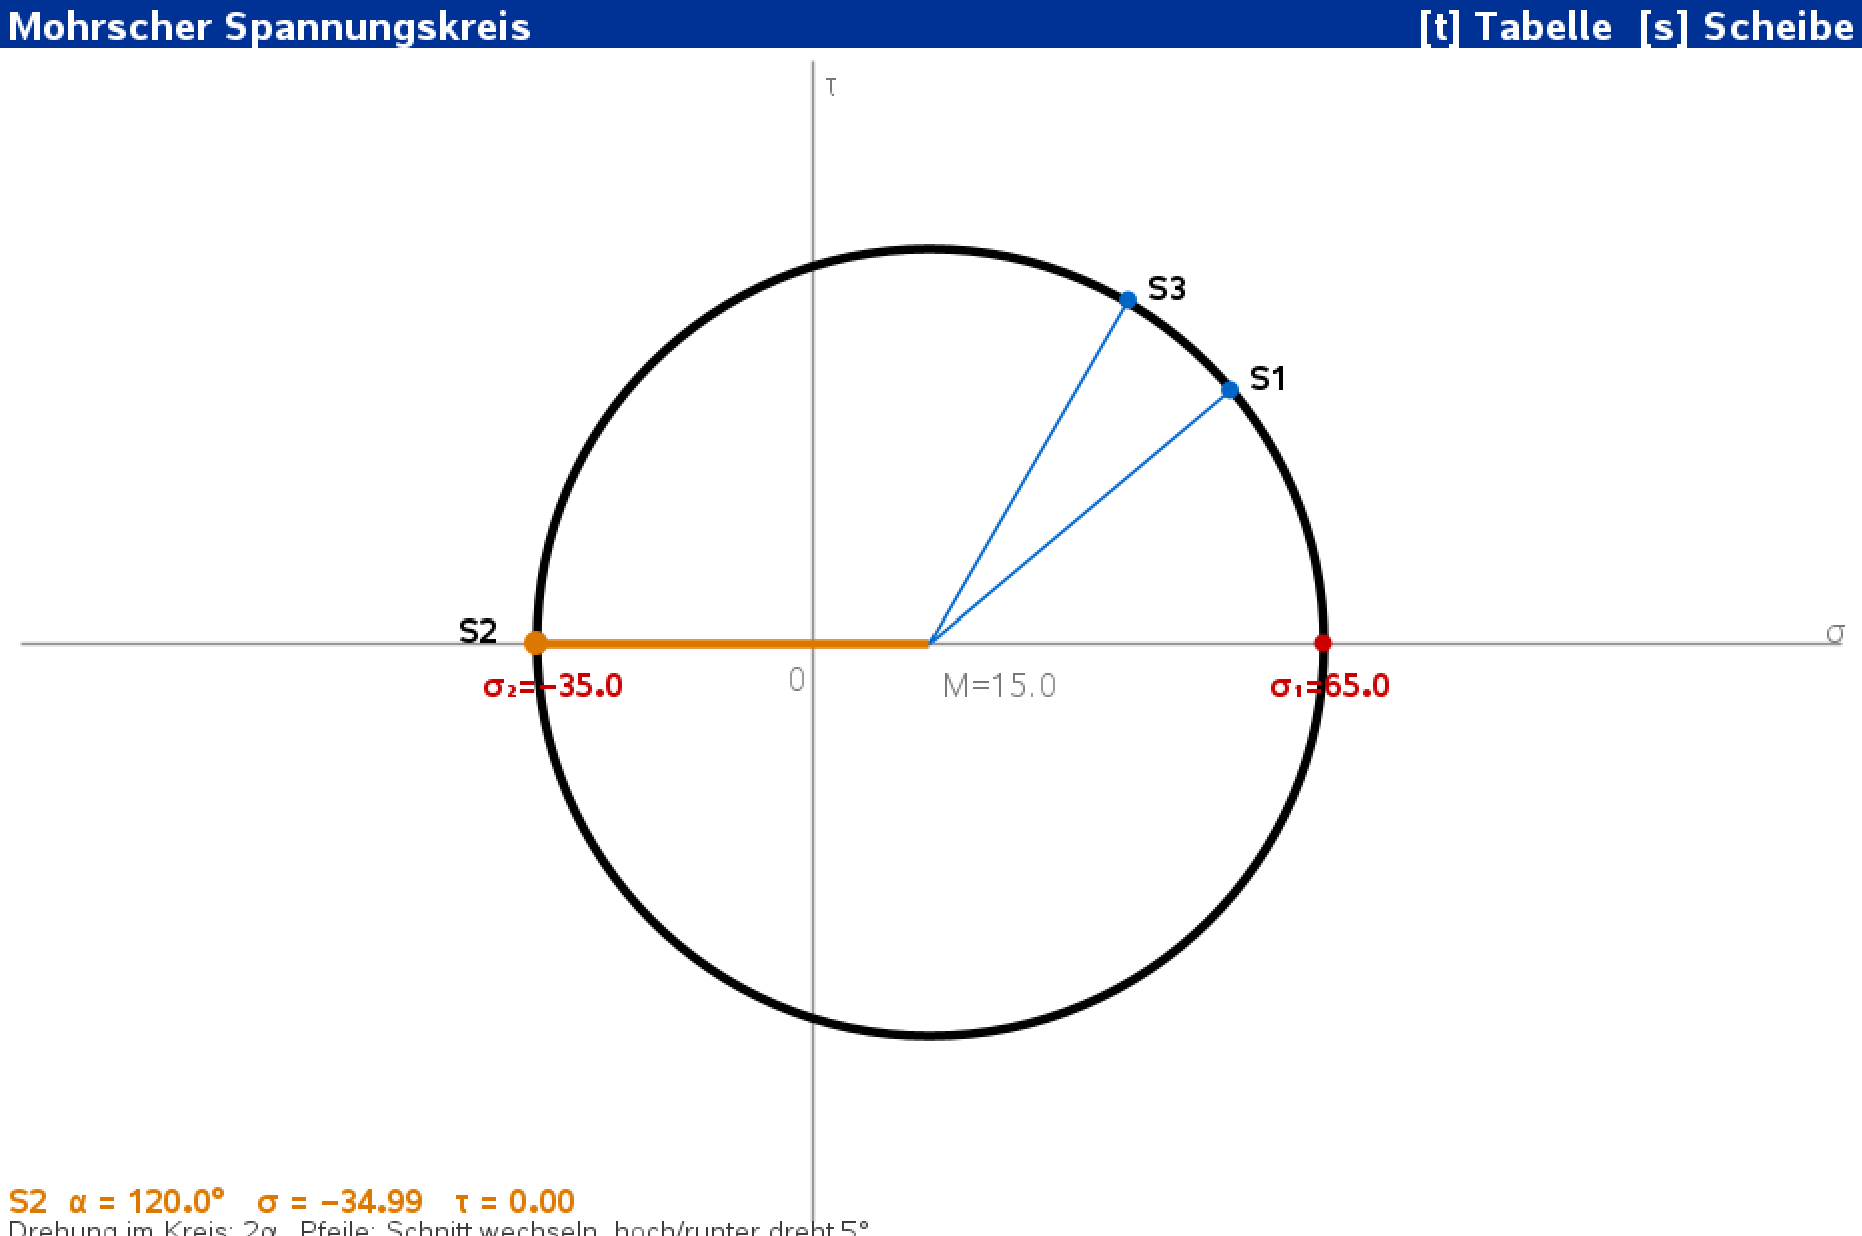
\includegraphics[width=\linewidth]{./fig/TM2/WiSe2122nr3_3.png}
        \caption{Spannungs-Kreis}
    \end{subfigure}
    \caption{Lösung von TM2 WiSe~21/22, Nr.~3}
    \label{fig:TM2WiSe2122Nr3_2}
\end{figure}

Falls bei einer Aufgabe nach dem Winkel eines Schnitts gefragt wird und das Programm zwei Winkel ausgibt, muss natürlich
geprüft werden, welcher Winkel eher zur Skizze passt.

\subsection{Schubspannung und SMP (TM2 SoSe 24 Nr.~8)}

\subsection{Verwölbung (TM2 SoSe 20 Nr.~9)} eingebunden.
% Hier keine \usepackage-Zeilen: Pakete stehen in der Praeambel von Anleitung.tex.
% Abbildungen mit [htbp]: LaTeX setzt sie dann dorthin, wo Platz ist. Im Text deshalb immer
% mit Abb.~\ref{...} auf sie verweisen, nicht mit "unten" oder "folgendermaßen".


\part{Beispiele}

In diesem Teil will ich anhand typischer Klausuraufgaben etwas genauer beschreiben, wie man das
Programm am besten verwendet, zumindest so, wie ich es für sinnvoll halte.

Die Screenshots habe ich in der PC-Ansicht gemacht, weil dort viele Dinge besser erkennbar sind.
Auf dem Taschenrechner selbst sollte mit Zoom aber auch alles erkennbar sein.

\section{TM1}
\subsection{WiSe~21/22}
\subsubsection{Geschlossenes System (Nr.~2)}
Bei dieser Aufgabe gibt es ein paar Besonderheiten bei der Eingabe, deshalb stelle ich sie hier vor.
Im Programm sieht das Tragwerk aus wie in Abb.~\ref{fig:WiSe2122nr2_1}.

\begin{figure}[htbp]
    \centering
    \begin{subfigure}[t]{0.48\textwidth}
        \centering
        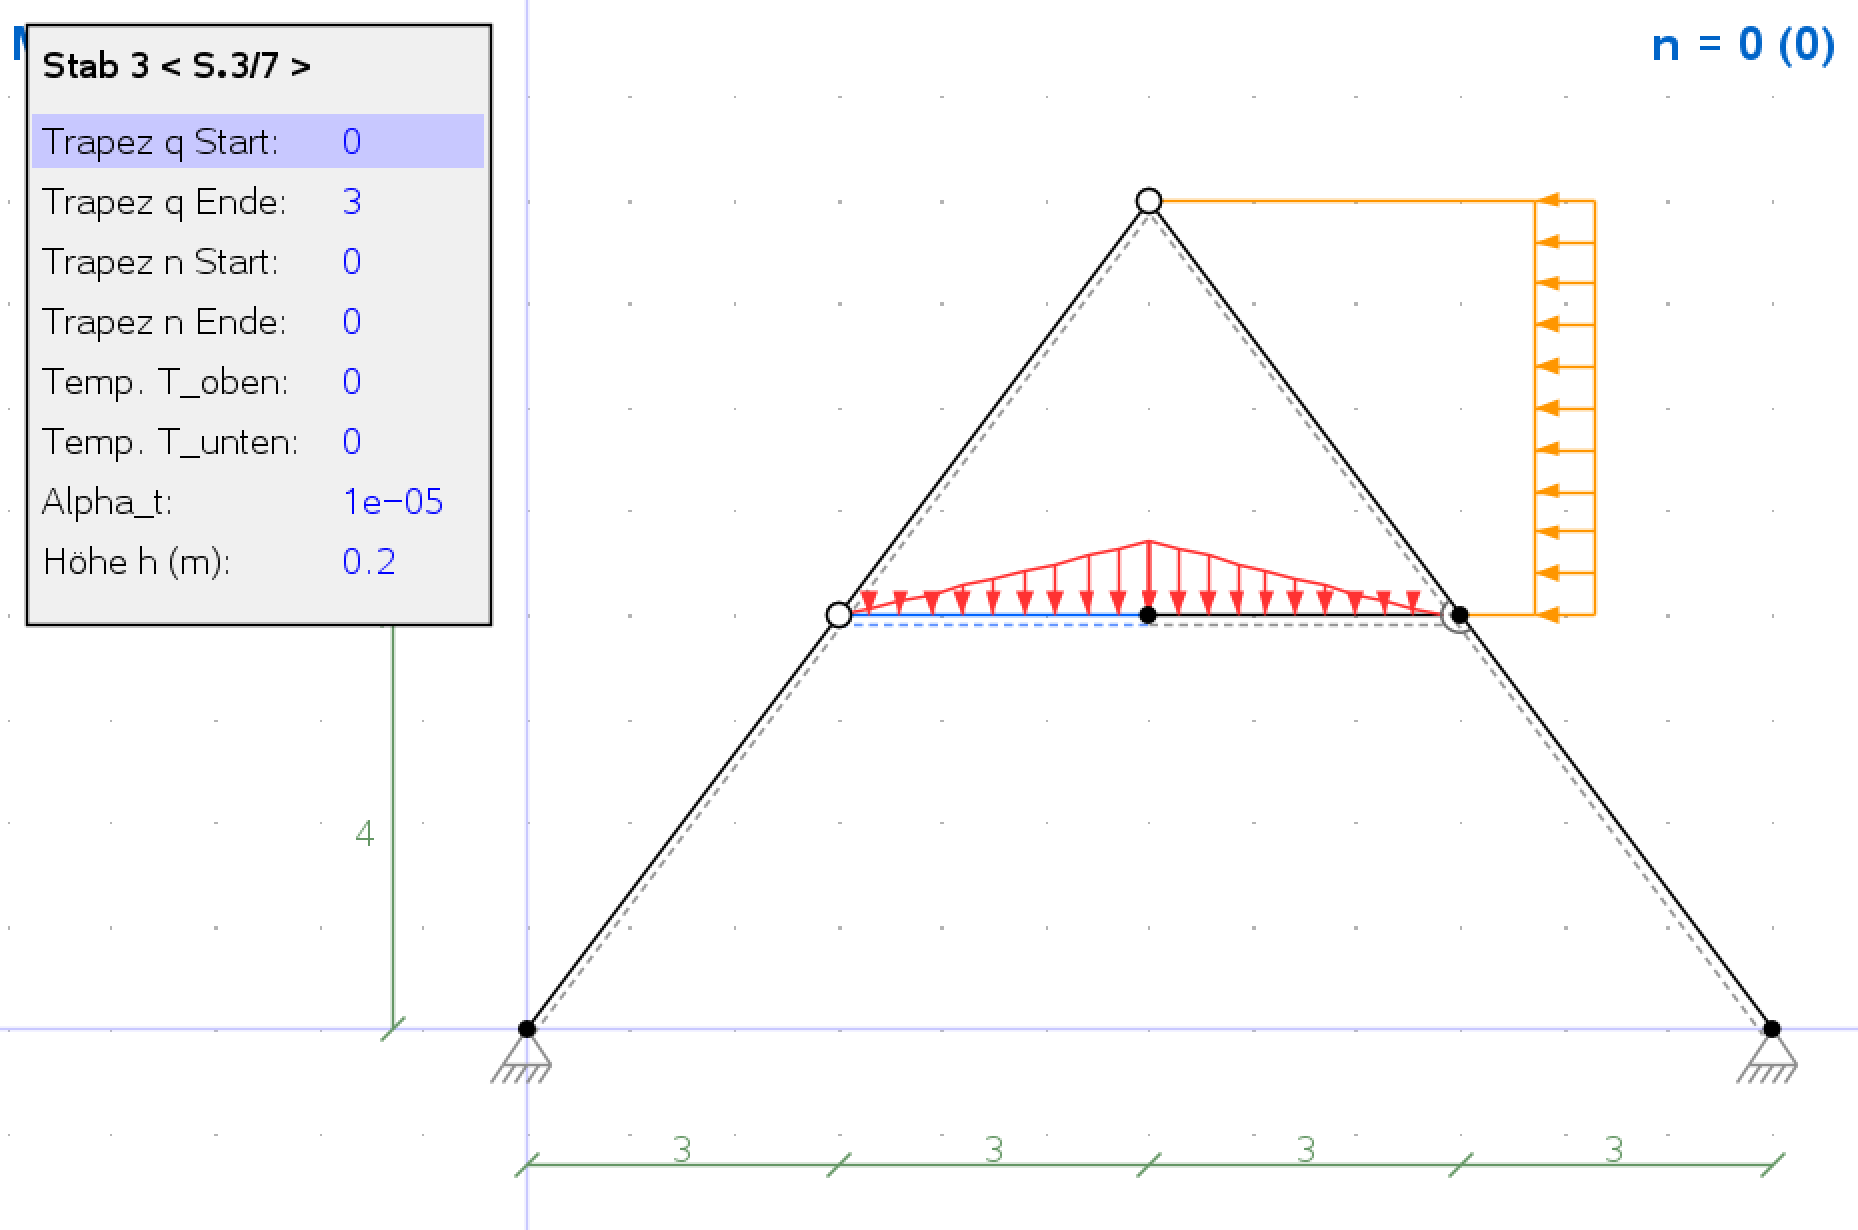
\includegraphics[width=\linewidth]{./fig/TM1/WiSe2122nr2_1.png}
        \caption{Trapezlast auf der linken Hälfte des Mittelstabs}
    \end{subfigure}
    \hfill
    \begin{subfigure}[t]{0.48\textwidth}
        \centering
        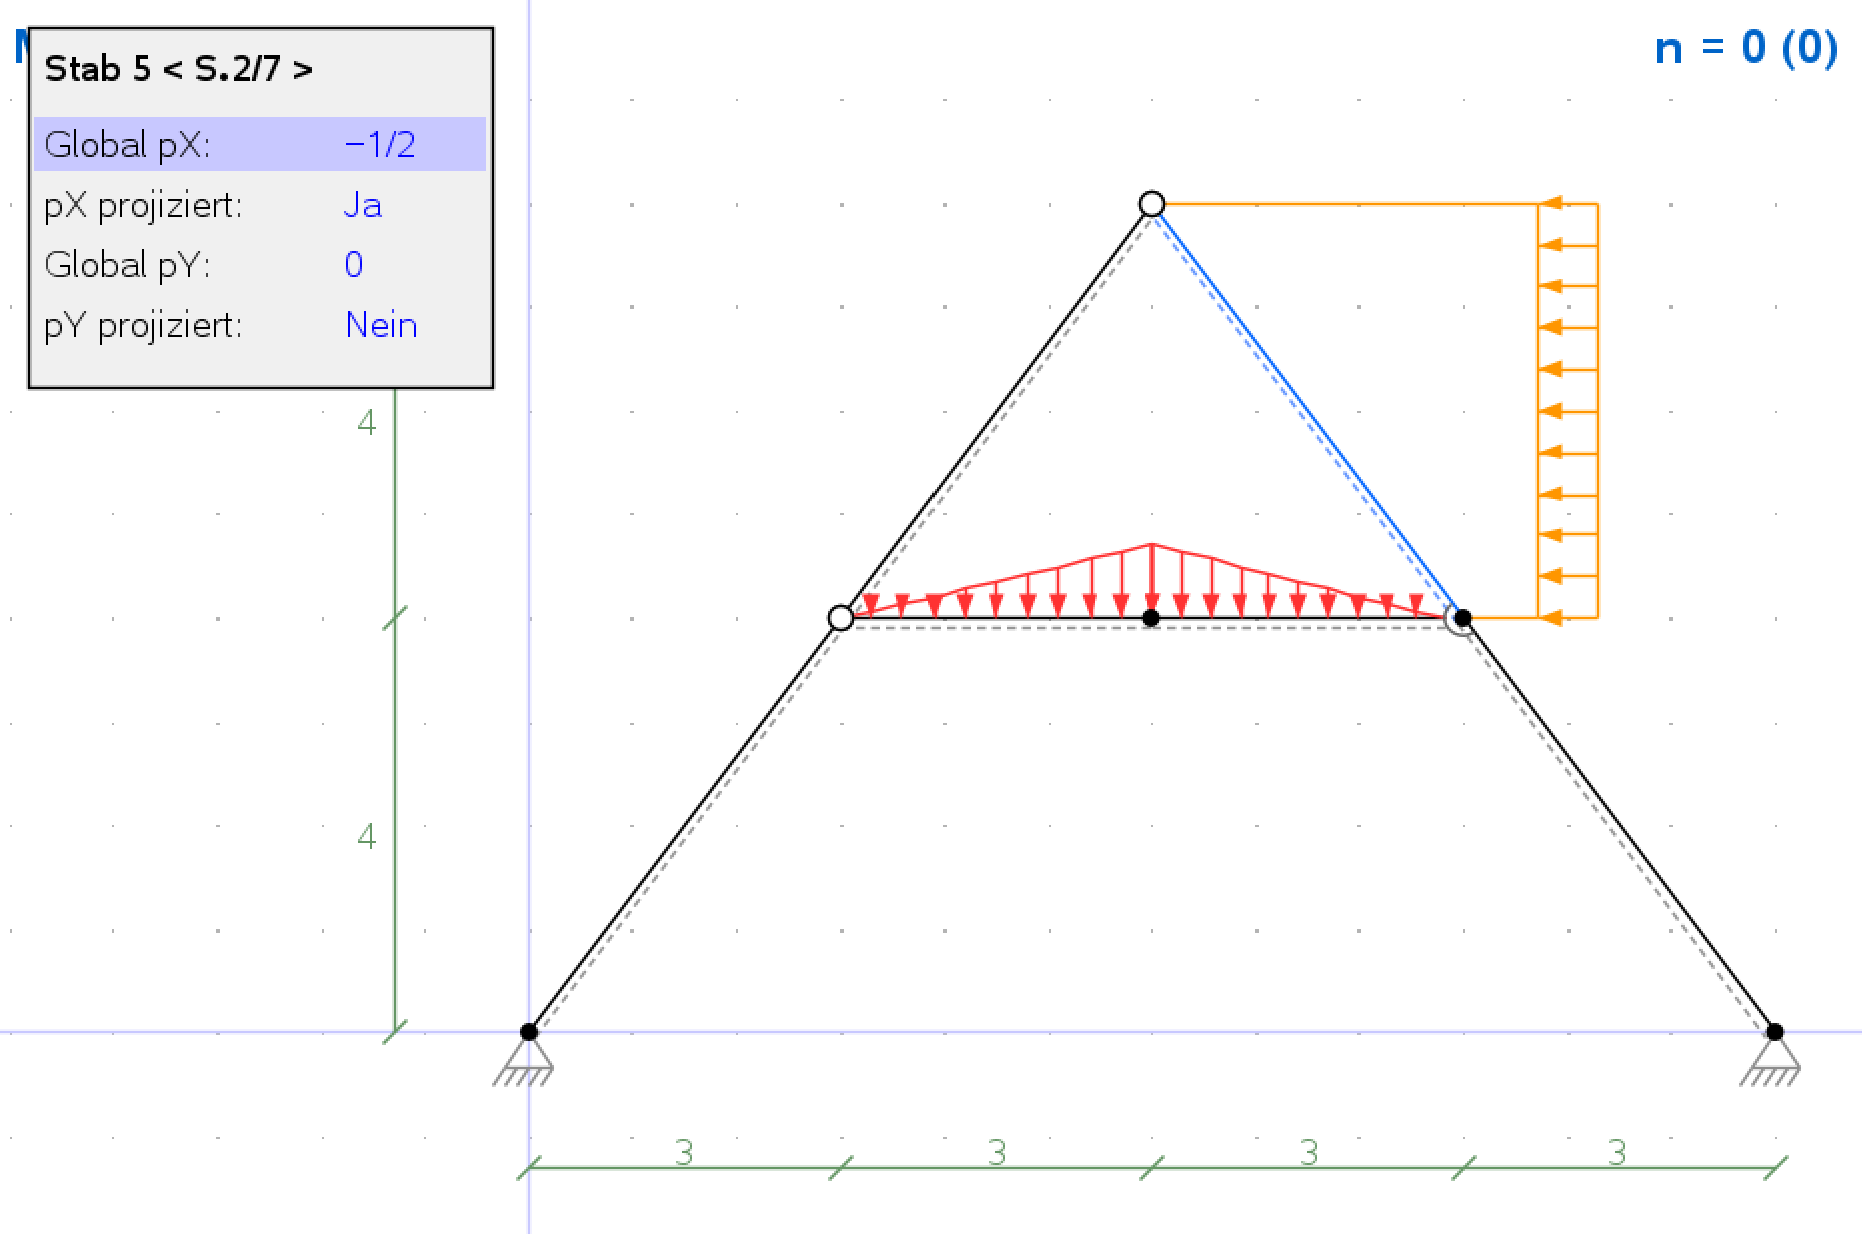
\includegraphics[width=\linewidth]{./fig/TM1/WiSe2122nr2_2.png}
        \caption{globale Streckenlast am oberen rechten Stab}
    \end{subfigure}
    \caption{WiSe~21/22, Nr.~2 im Programm}
    \label{fig:WiSe2122nr2_1}
\end{figure}

Den Stab in der Mitte müsst ihr im Programm teilen. Die Last auf ihm ist dreieckförmig mit der
Spitze in der Mitte, eine Trapezlast geht aber immer über einen ganzen Stab. Jede Hälfte bekommt
deshalb ihre eigene Trapezlast, die linke von $0$ auf $3$, die rechte von $3$ auf $0$
(Abb.~\ref{fig:WiSe2122nr2_1}a). Der neue Knoten in der Mitte bleibt biegesteif.

Die Streckenlast am schrägen Stab gebt ihr am einfachsten als globale Last ein
(Abb.~\ref{fig:WiSe2122nr2_1}b). In der Aufgabe ist sie auf die senkrechte Projektion des Stabes
bezogen, deshalb muss \emph{pX projiziert} auf \emph{Ja} stehen. Negativ ist sie, weil sie global
gesehen entgegen der $x$-Achse wirkt, also nach links.

Nach dem Berechnen könnt ihr das LGS, das zur Explosionsansicht (Abb.~\ref{fig:WiSe2122nr2_2})
gehört, über die zweite Seite des Obermenüs (\emph{LGS-Matrix}) in den Taschenrechner exportieren
(Abb.~\ref{fig:WiSe2122nr2_3}). Die Gleichungen stehen dann lesbar in \code{lgs}, die Lösung
bekommt ihr zum Beispiel mit \code{ggw\_x = ggw\_a$^{-1}$*ggw\_b}
(Abschnitt~\ref{sec:lgs-matrix}).

\begin{figure}[htbp]
    \centering
    \begin{subfigure}[t]{0.48\textwidth}
        \centering
        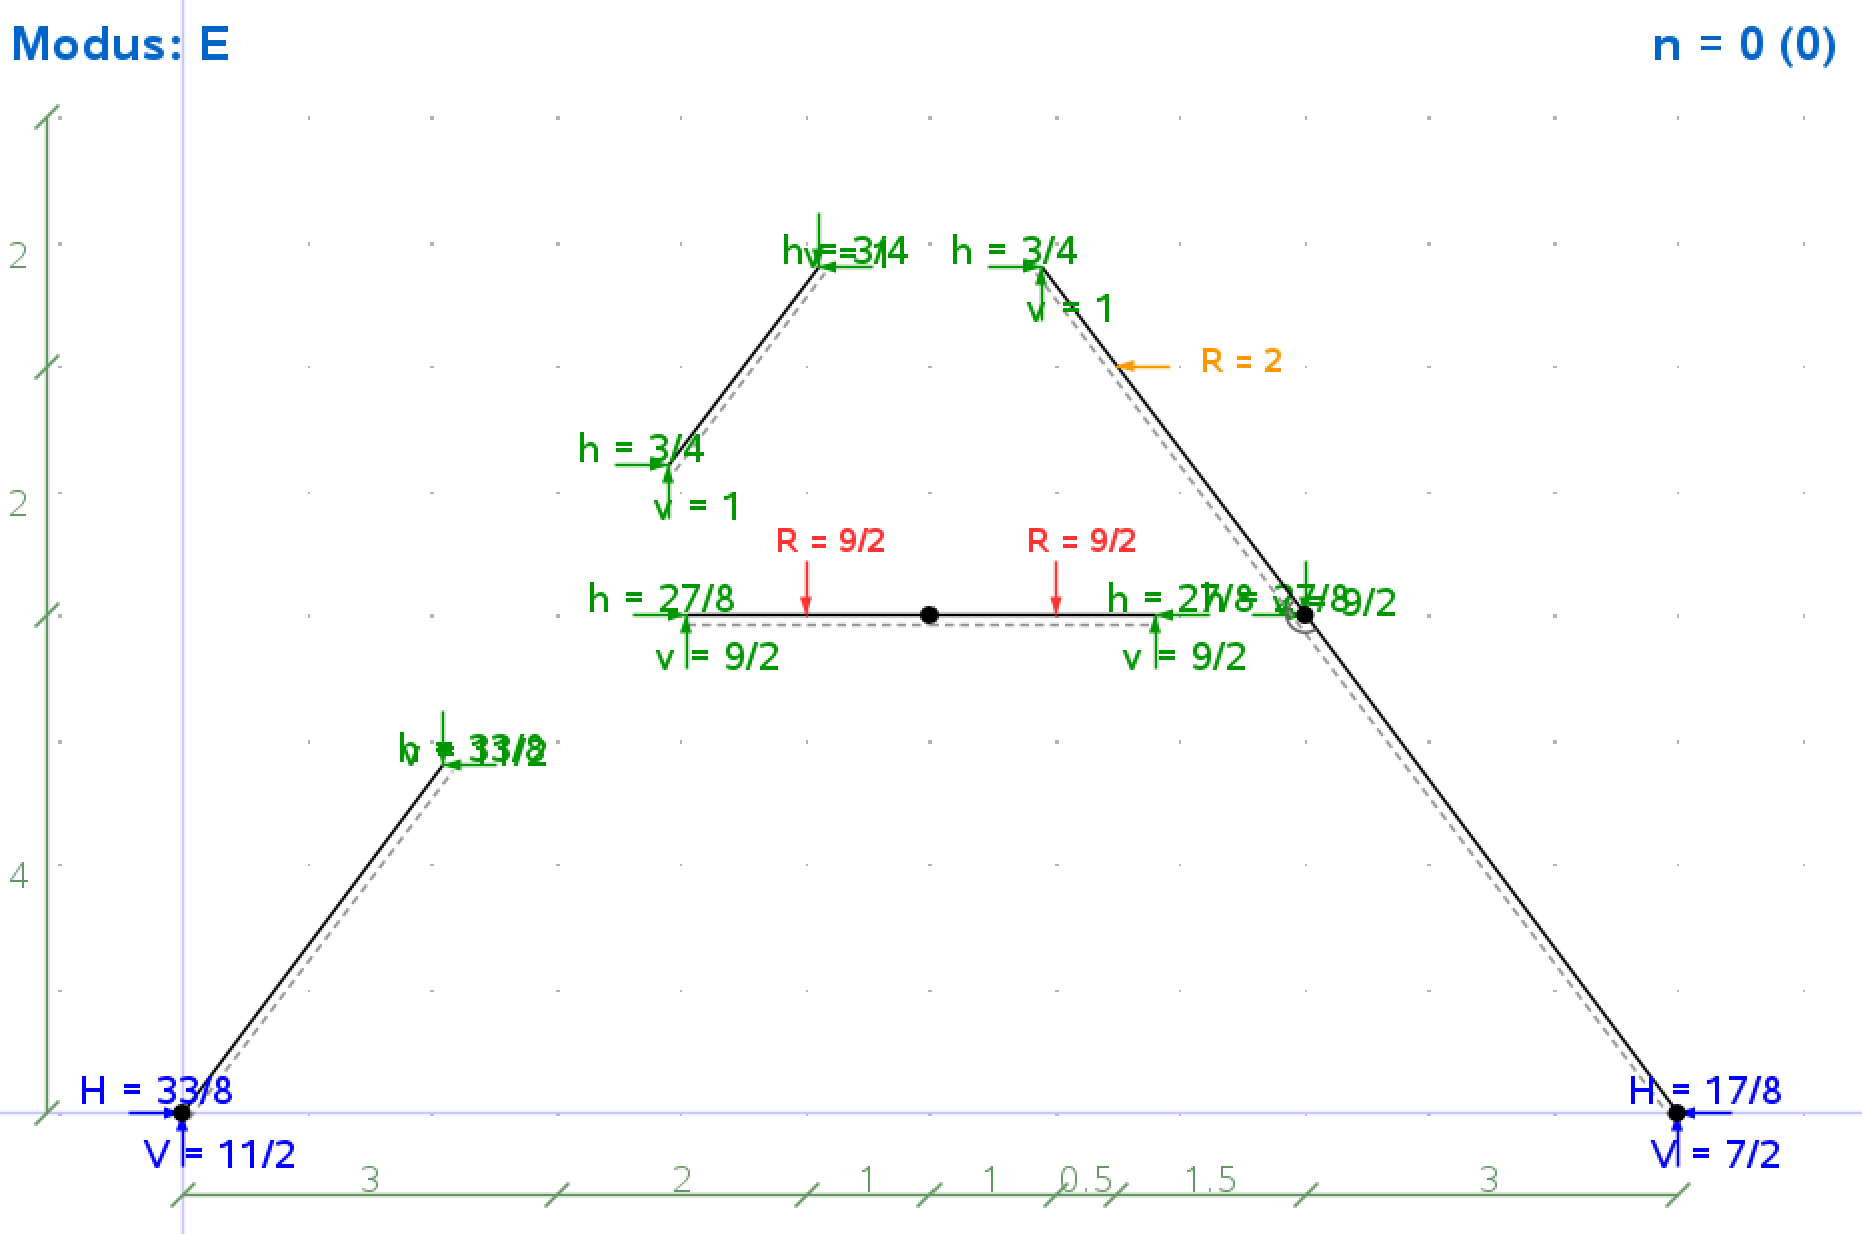
\includegraphics[width=\linewidth]{./fig/TM1/WiSe2122nr2_5.png}
        \caption{Seite~1: Ergebnisse in ihrer wirklichen Richtung}
    \end{subfigure}
    \hfill
    \begin{subfigure}[t]{0.48\textwidth}
        \centering
        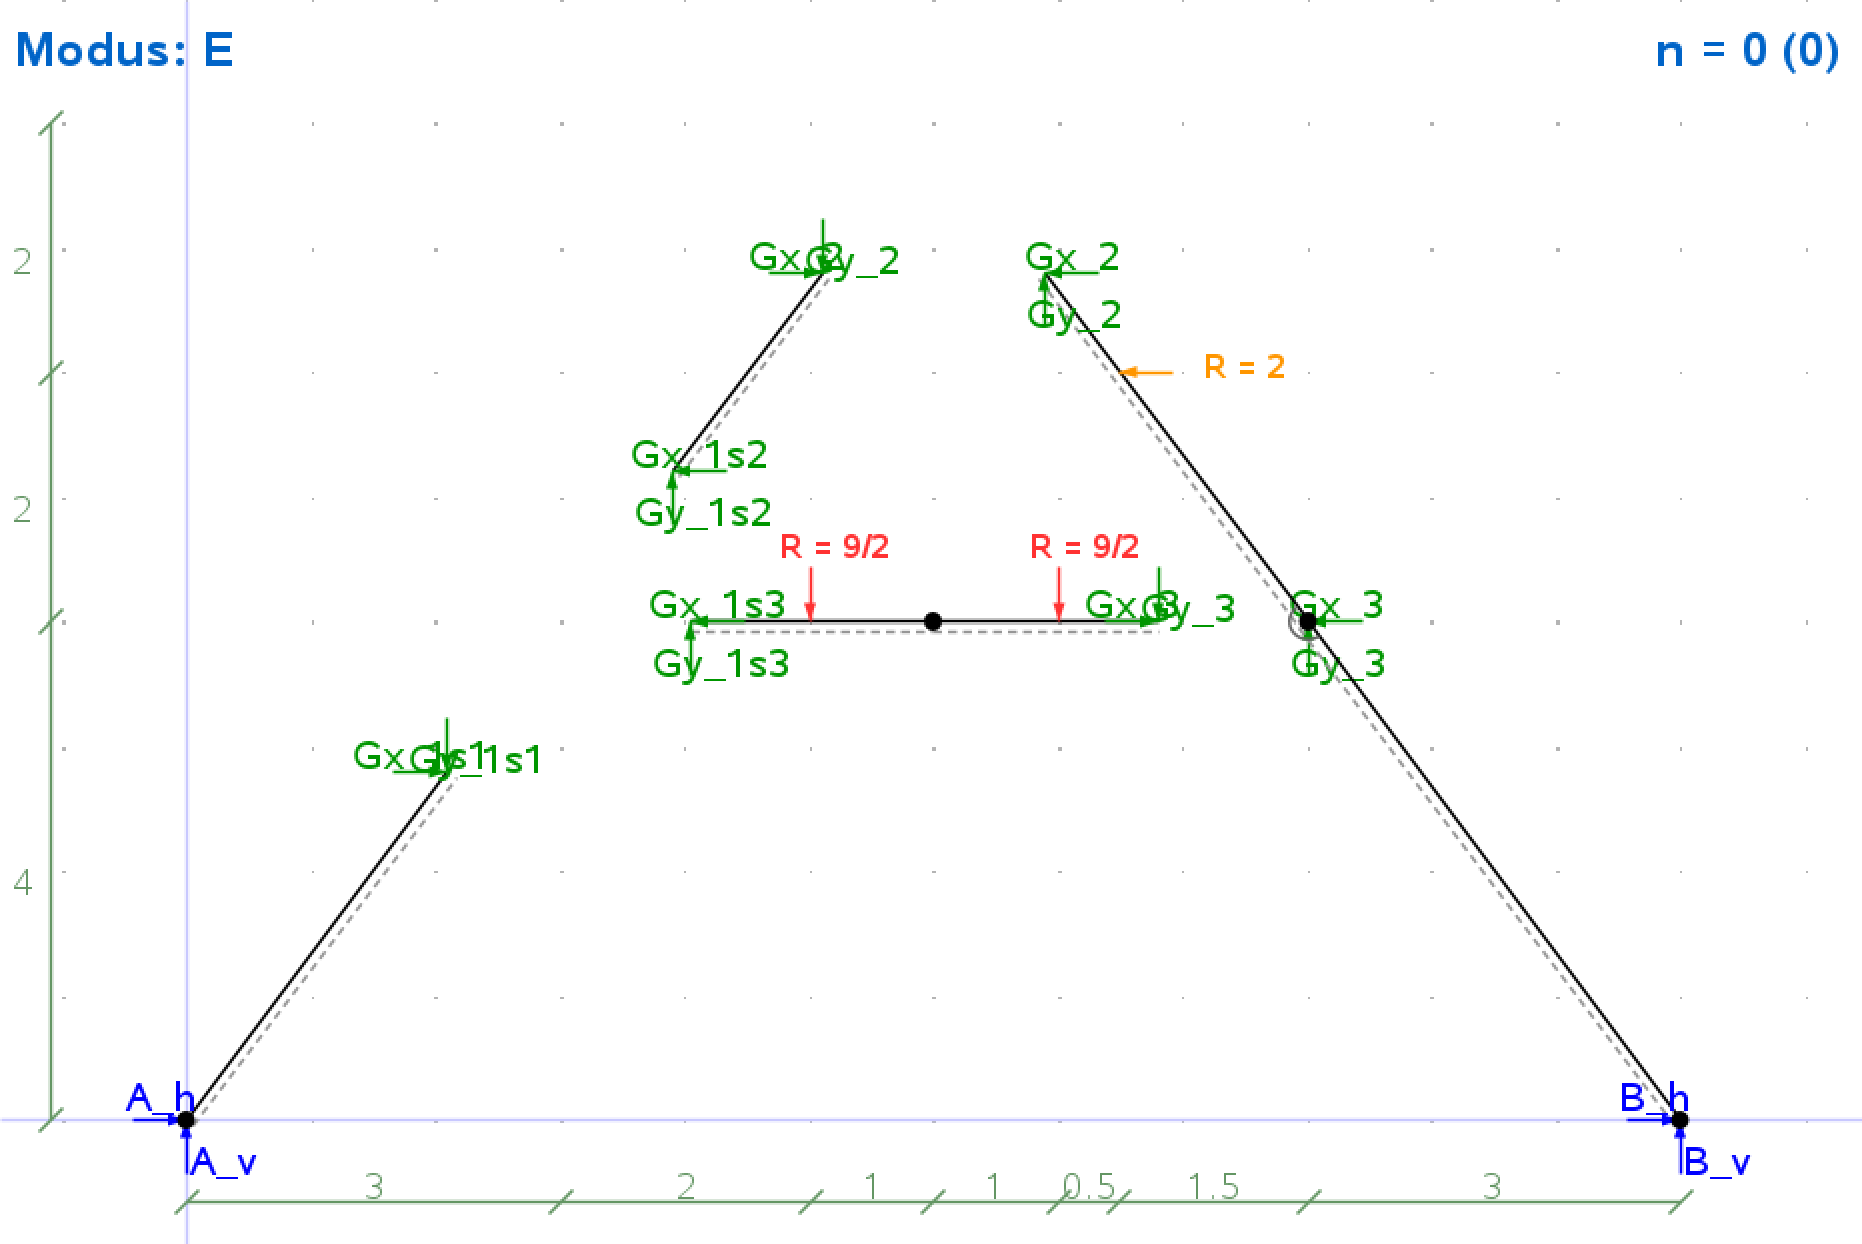
\includegraphics[width=\linewidth]{./fig/TM1/WiSe2122nr2_6.png}
        \caption{Seite~2: Unbekannte in positiver Richtung}
    \end{subfigure}
    \caption{WiSe~21/22, Nr.~2: Explosionsansicht (E-Modus)}
    \label{fig:WiSe2122nr2_2}
\end{figure}

\begin{figure}[htbp]
    \centering
    \begin{subfigure}[t]{0.48\textwidth}
        \centering
        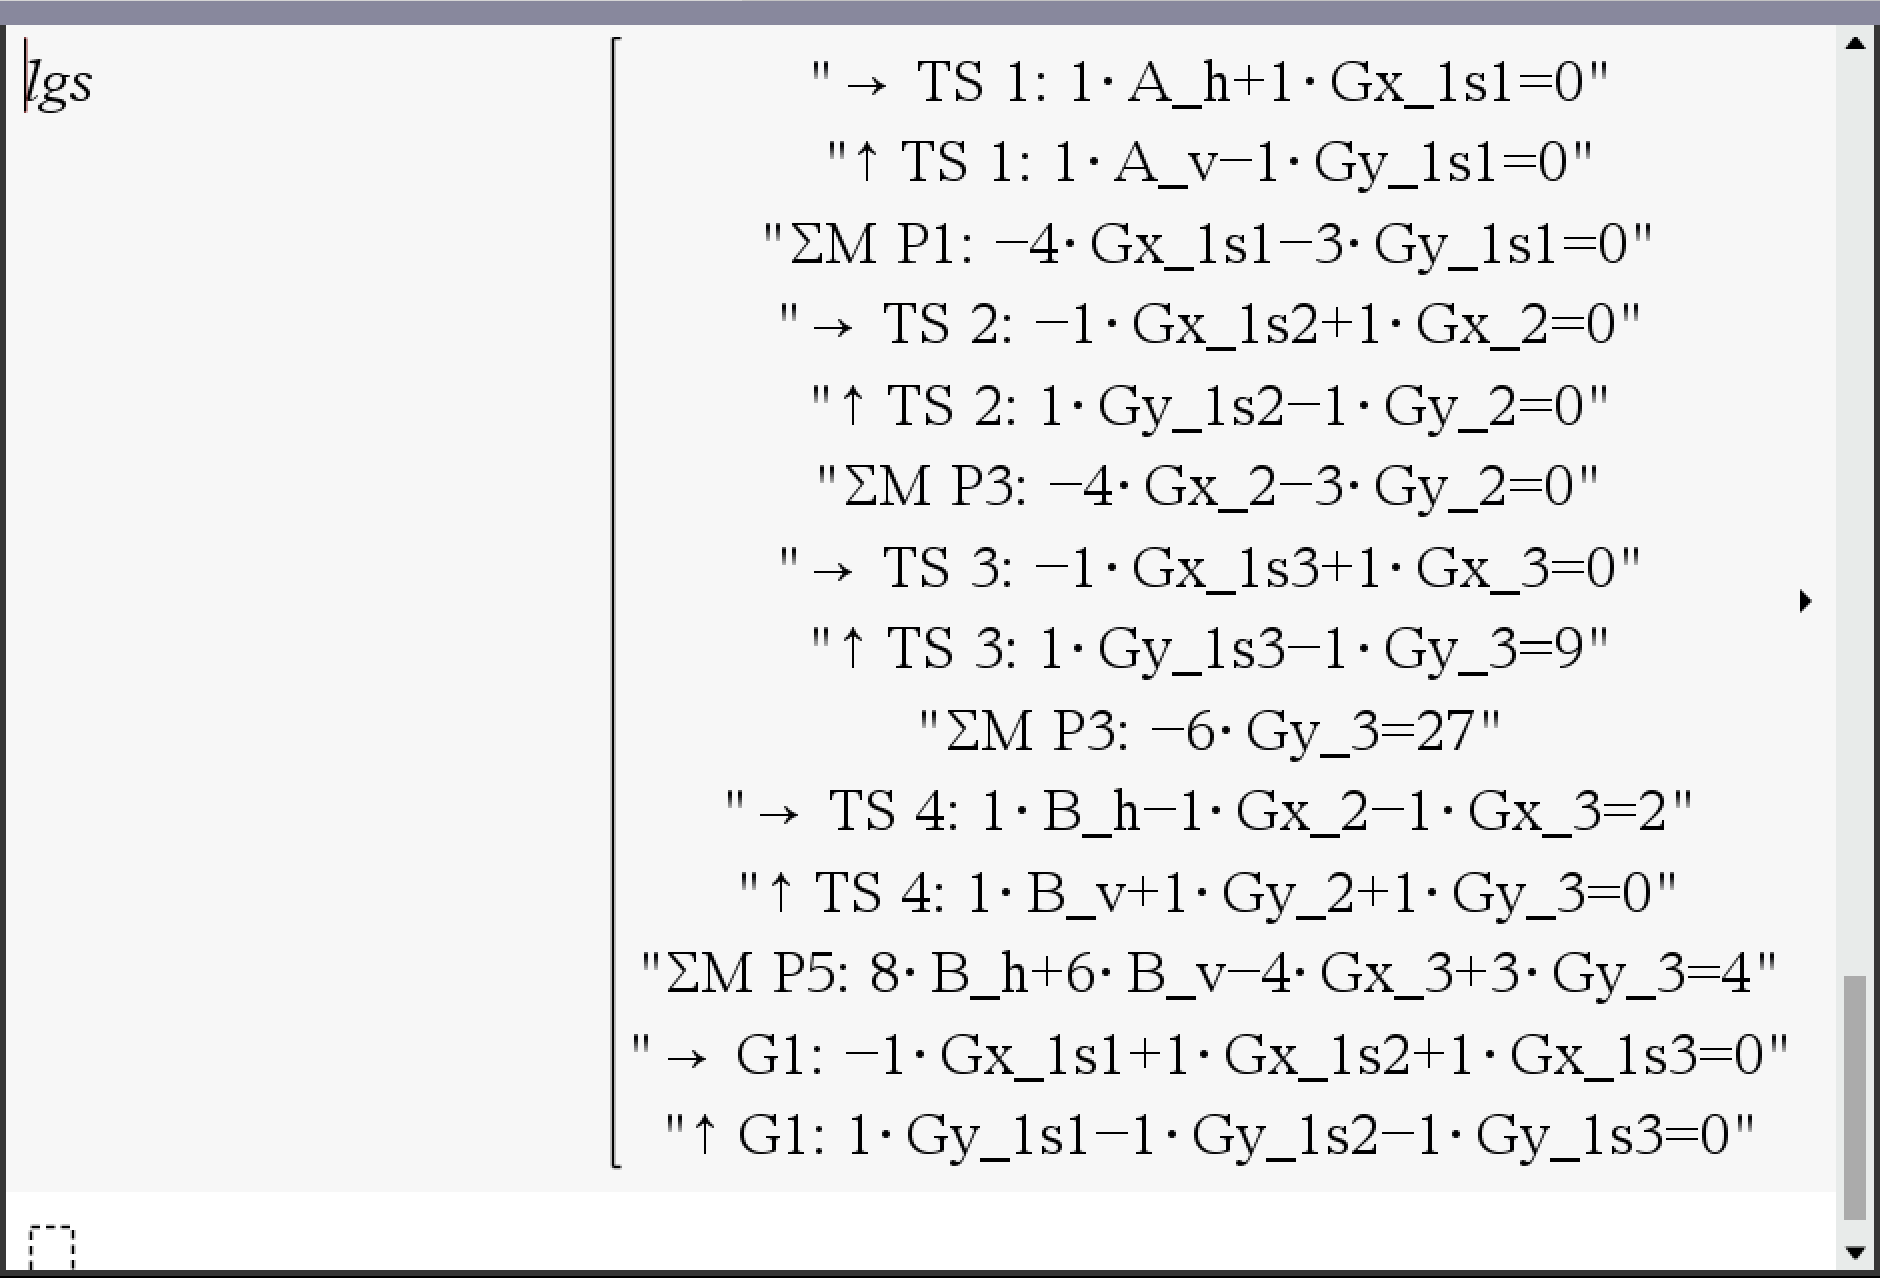
\includegraphics[width=\linewidth]{./fig/TM1/WiSe2122nr2_3.png}
        \caption{exportierte Gleichungen \code{lgs}}
    \end{subfigure}
    \hfill
    \begin{subfigure}[t]{0.48\textwidth}
        \centering
        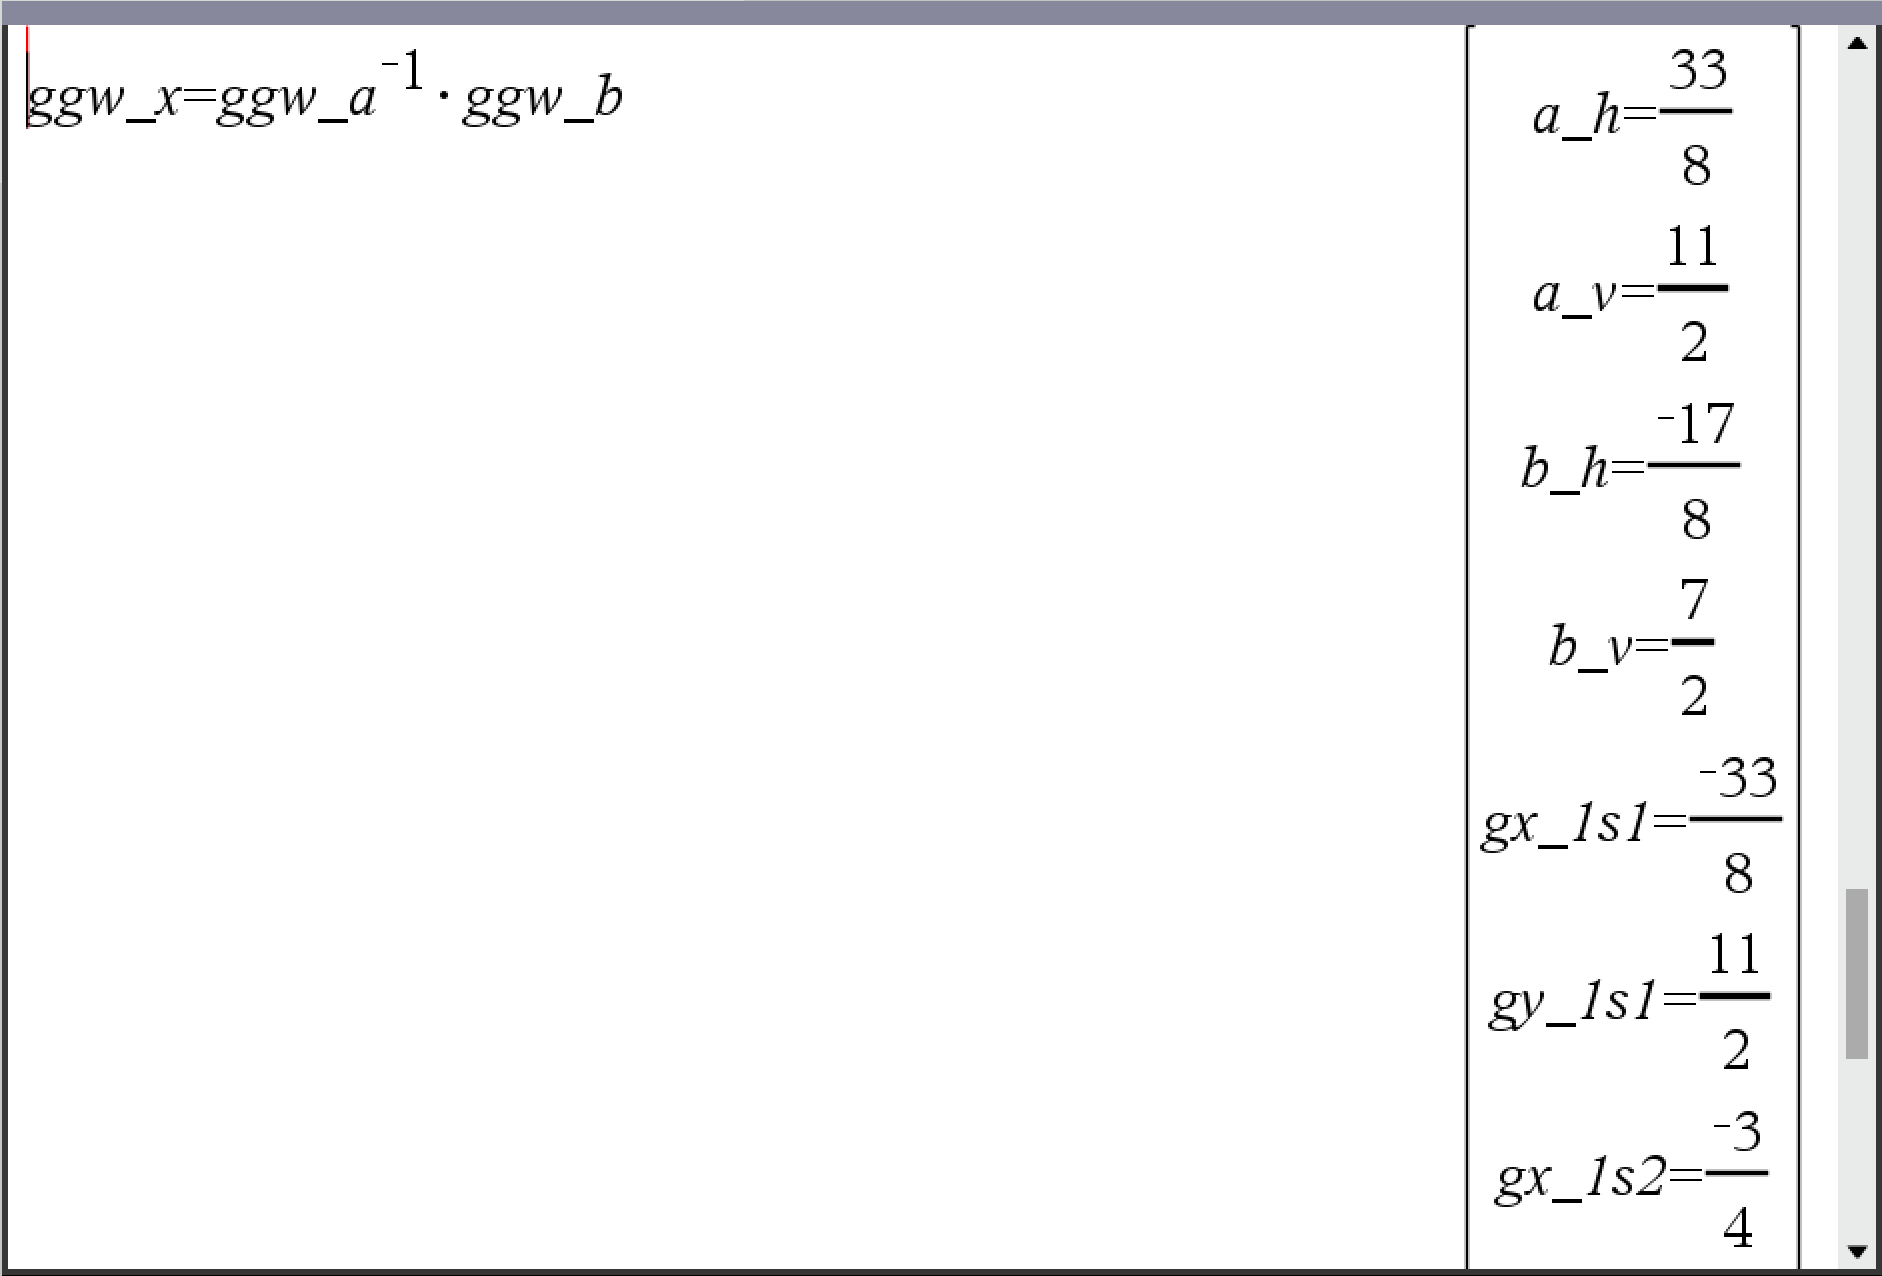
\includegraphics[width=\linewidth]{./fig/TM1/WiSe2122mr2_4.png}
        \caption{Lösung mit \code{ggw\_x}}
    \end{subfigure}
    \caption{WiSe~21/22, Nr.~2: exportiertes LGS}
    \label{fig:WiSe2122nr2_3}
\end{figure}

Die Explosionsansicht kann manchmal etwas unübersichtlich sein. Wenn ihr nah genug heranzoomt,
sollte aber trotzdem alles erkennbar sein. Die Ergebnisse müsst ihr natürlich nicht in dieser
Vektorform aufschreiben, nur ihr Inhalt zählt.

An dieser Stelle will ich anmerken, dass meist nur bei Systemen mit einem geschlossenen Ring wie
diesem nach allen Gelenk- und Auflagerkräften gefragt wird. Bei offenen Systemen ohne Ring wird oft
nur nach den Auflagerkräften gefragt. Das exportierte LGS liefert dann zwar auch die richtige Lösung, ist aber
meist mehr, als ihr braucht. Den Punkt, um den das Programm die Momentensumme eines Teilsystems
bildet, seht ihr, wenn ihr in der Explosionsansicht mit der Maus über das Teilsystem fahrt
(\emph{Hover}).

Die Zustandslinien, also die Verläufe der Schnittgrößen, zeichnet euch das Programm mit den Tasten
\taste{n}, \taste{q} und \taste{m}, die könnt ihr einfach abzeichnen. Falls ihr Randwerte schlecht
erkennt, fahrt mit der Maus über den jeweiligen Stab, dann zeigt das Programm nur noch diesen Stab
mit seinen Randwerten an.

\subsubsection{Qualitavtive Verläufe im symbolischen Modus (Nr.~4)}

Um meinen den oben genannten Punkt zum symbolischen Modus zu verdeutlichen will ich hier kurz auf Teilaufgabe b) eingehen.
Das System und der Querkraftverlauf sind in Abbildung~\ref{fig:TM1WiSe2122Nr4} dargestellt.

\begin{figure}[htbp]
    \centering
    \begin{subfigure}[t]{0.48\textwidth}
        \centering
        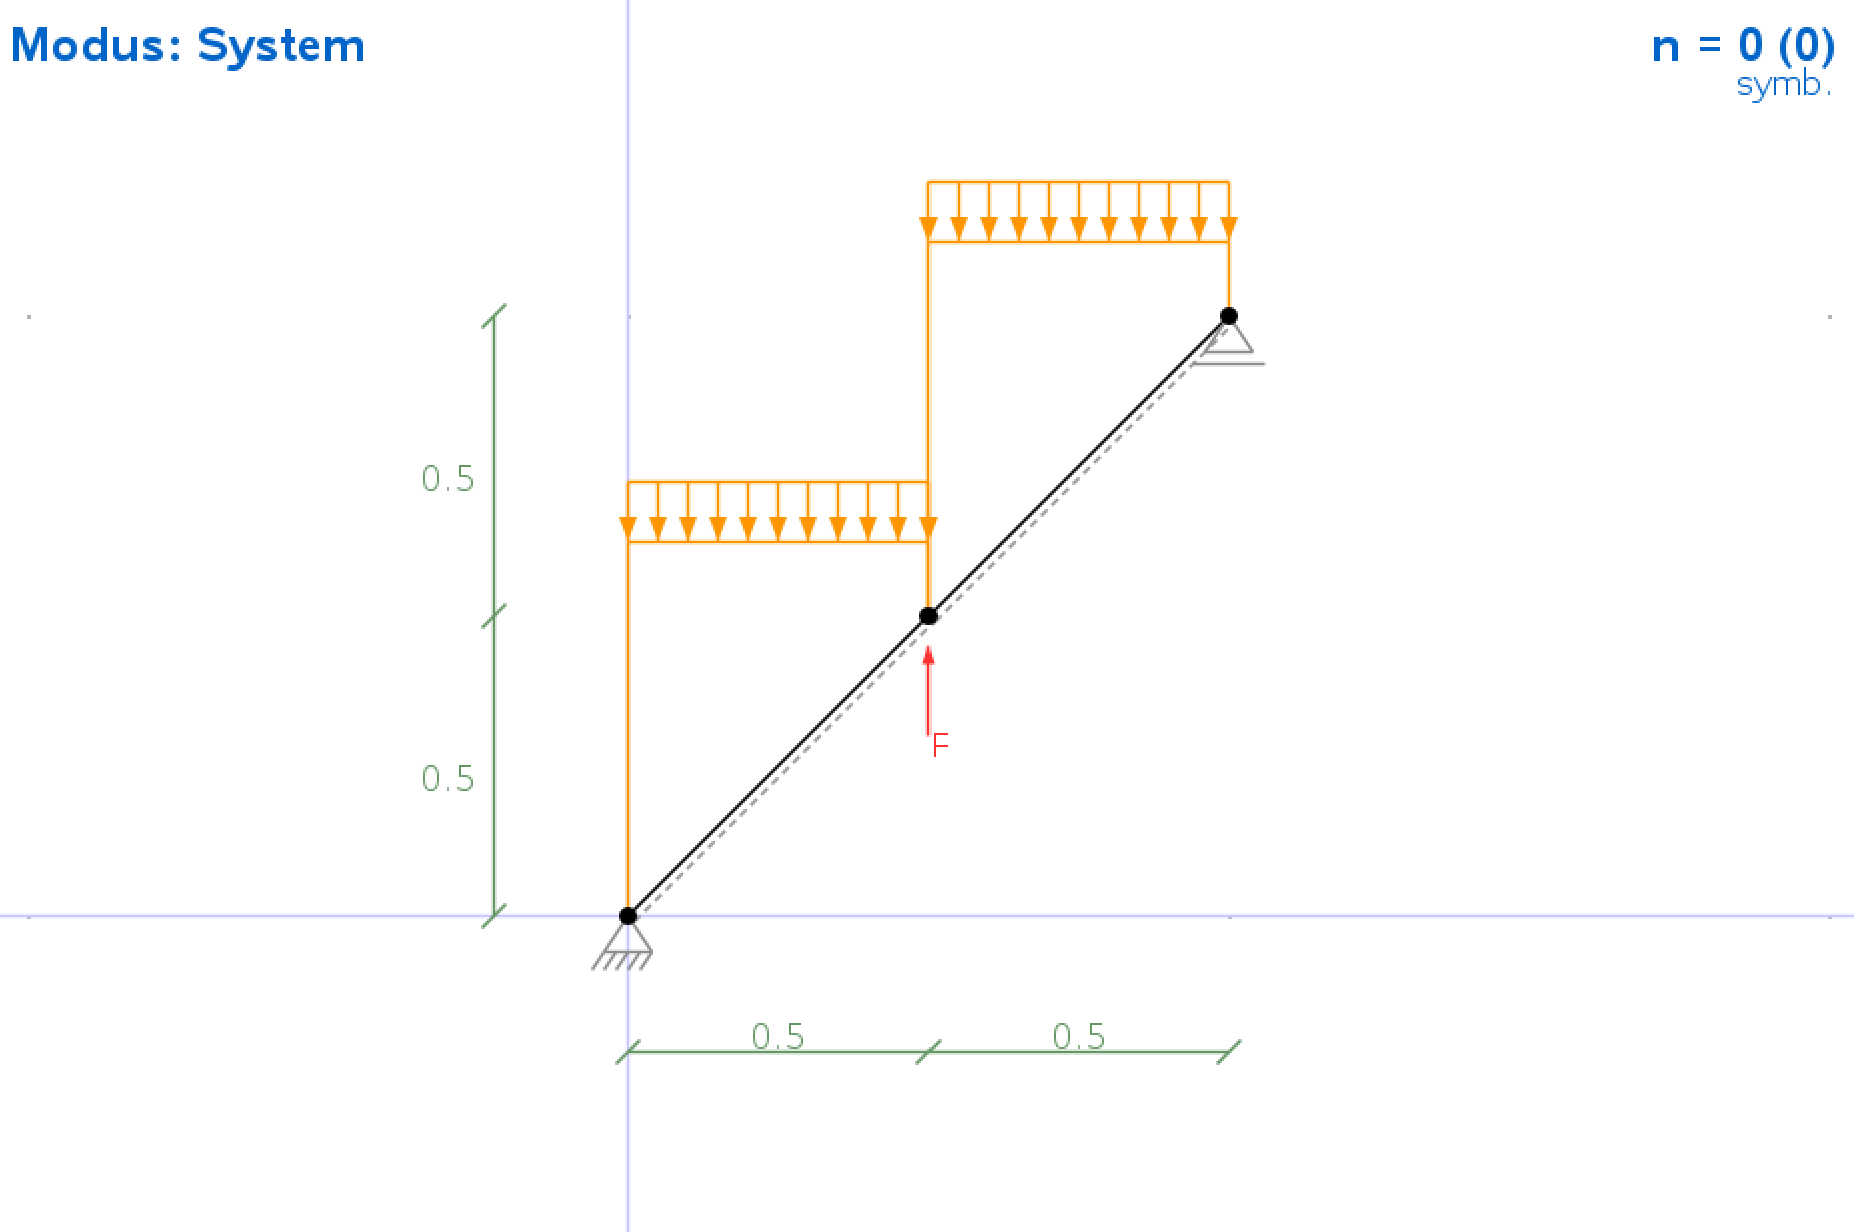
\includegraphics[width=\linewidth]{./fig/TM1/WiSe2122nr4_1.png}
        \caption{System}
    \end{subfigure}
    \hfill
    \begin{subfigure}[t]{0.48\textwidth}
        \centering
        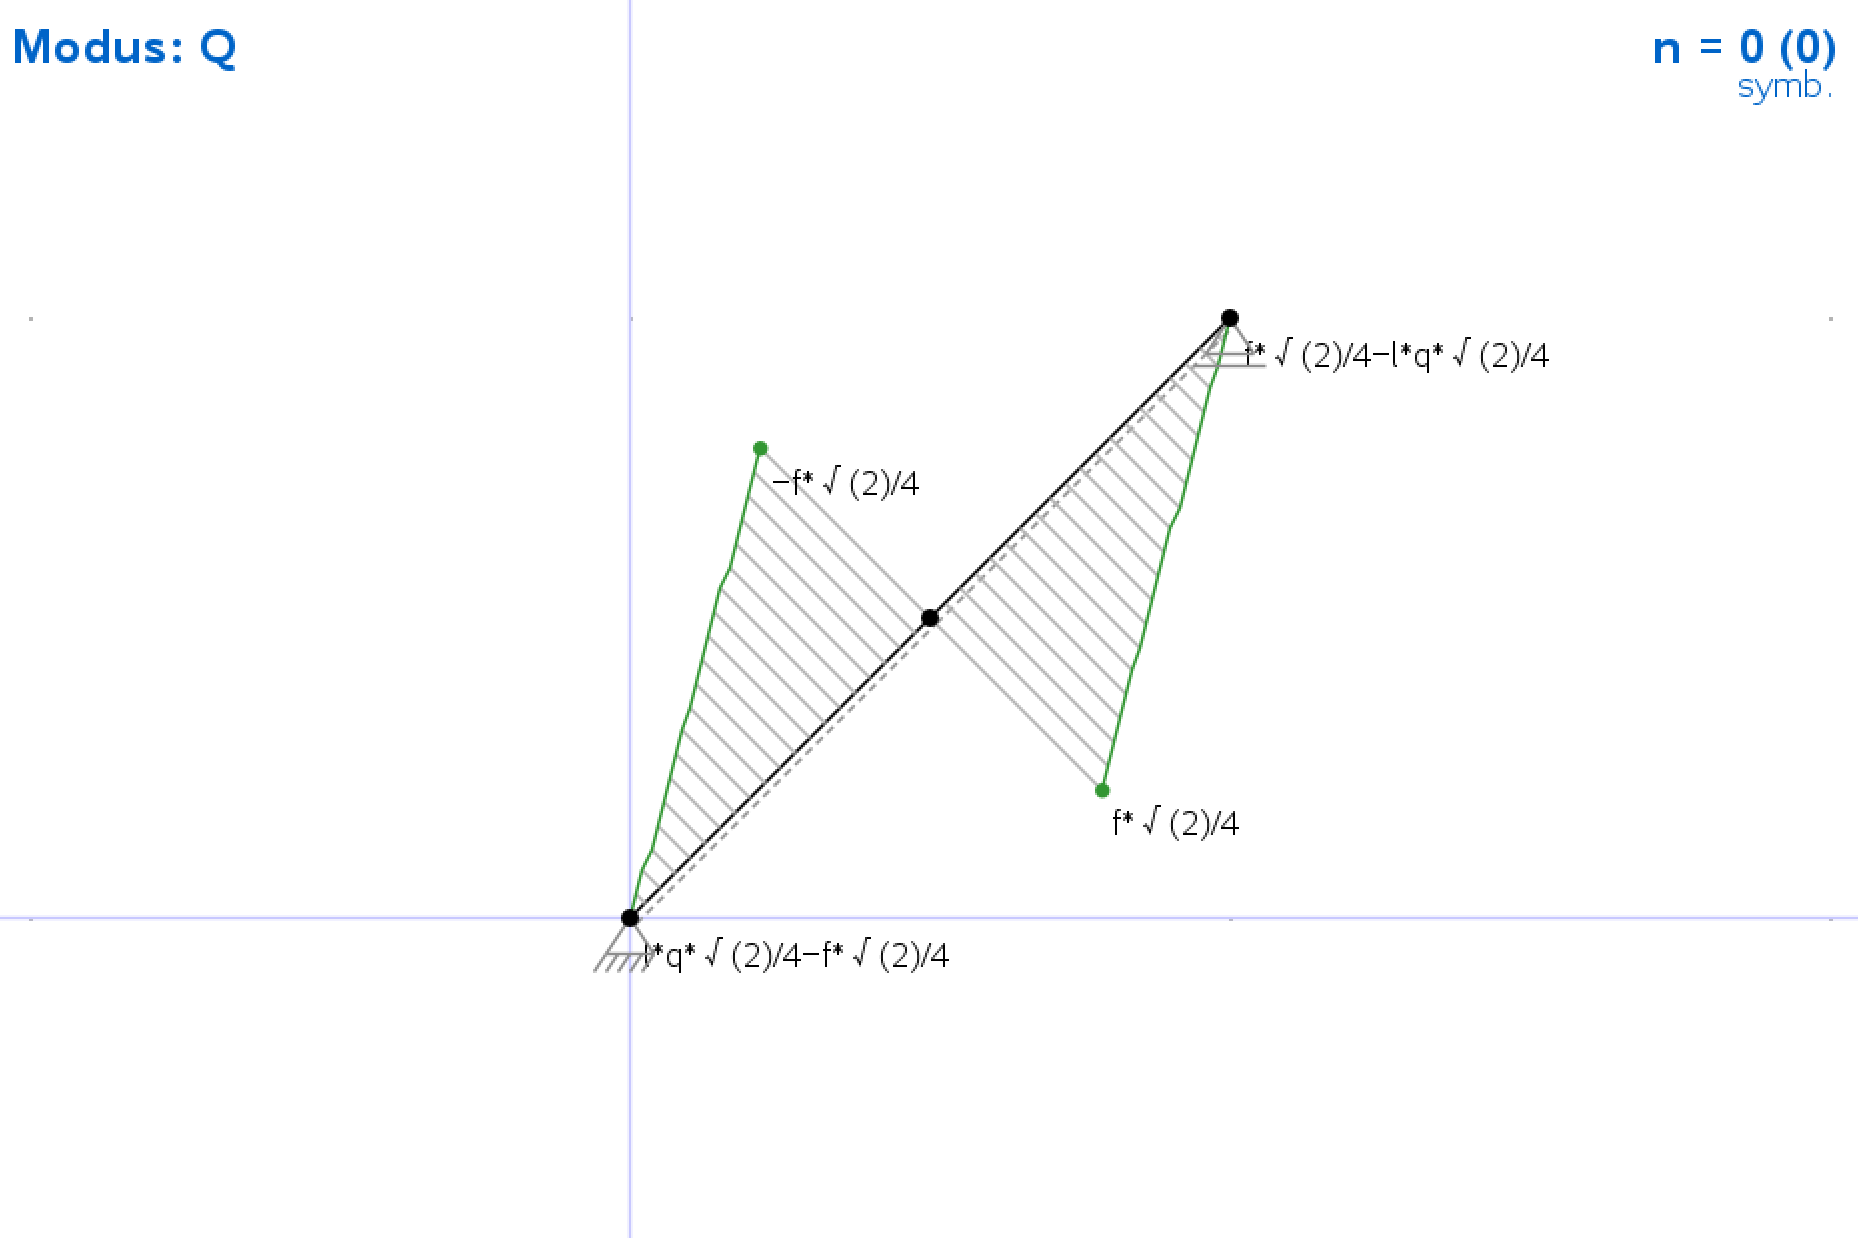
\includegraphics[width=\linewidth]{./fig/TM1/WiSe2122nr4_2.png}
        \caption{Querkraftverlauf}
    \end{subfigure}
    \caption{WiSe~21/22, Nr.~4}
    \label{fig:TM1WiSe2122Nr4}
\end{figure}

Im Querkraft verlauf sieht es so aus, als ob diese an den Auflagern null wird. Wenn man sich die Beschriftung der Randwerte 
anschaut wird jedoch klar, dass ist nur der Fall, wenn $q\cdot l=F$ bzw. $q\cdot a=F$ gilt. Das ist eben genau die Annhame des Programms,
um überhaupt irgendeinen Verlauf zeichnen zu können.
Die Aufgabe gibt aber unten vor: $F>q\cdot a$. Damit wird die Qerkraft am linekn Ende negativ und am rechten Ende positiv.
Die Verläufe von symbolische Berechnungen solltet ihr also \textbf{nie} einfach blind abzeichnen.

\subsection{PvV (Nr.~3)}

Zum PvV gibt es eigentlich nicht viel zu sagen. System zeichnen, \taste{v} drücken, Bindung wählen, abzeichnen,
dann exportieren und aufschreiben. 


\begin{figure}[htbp]
    \centering
    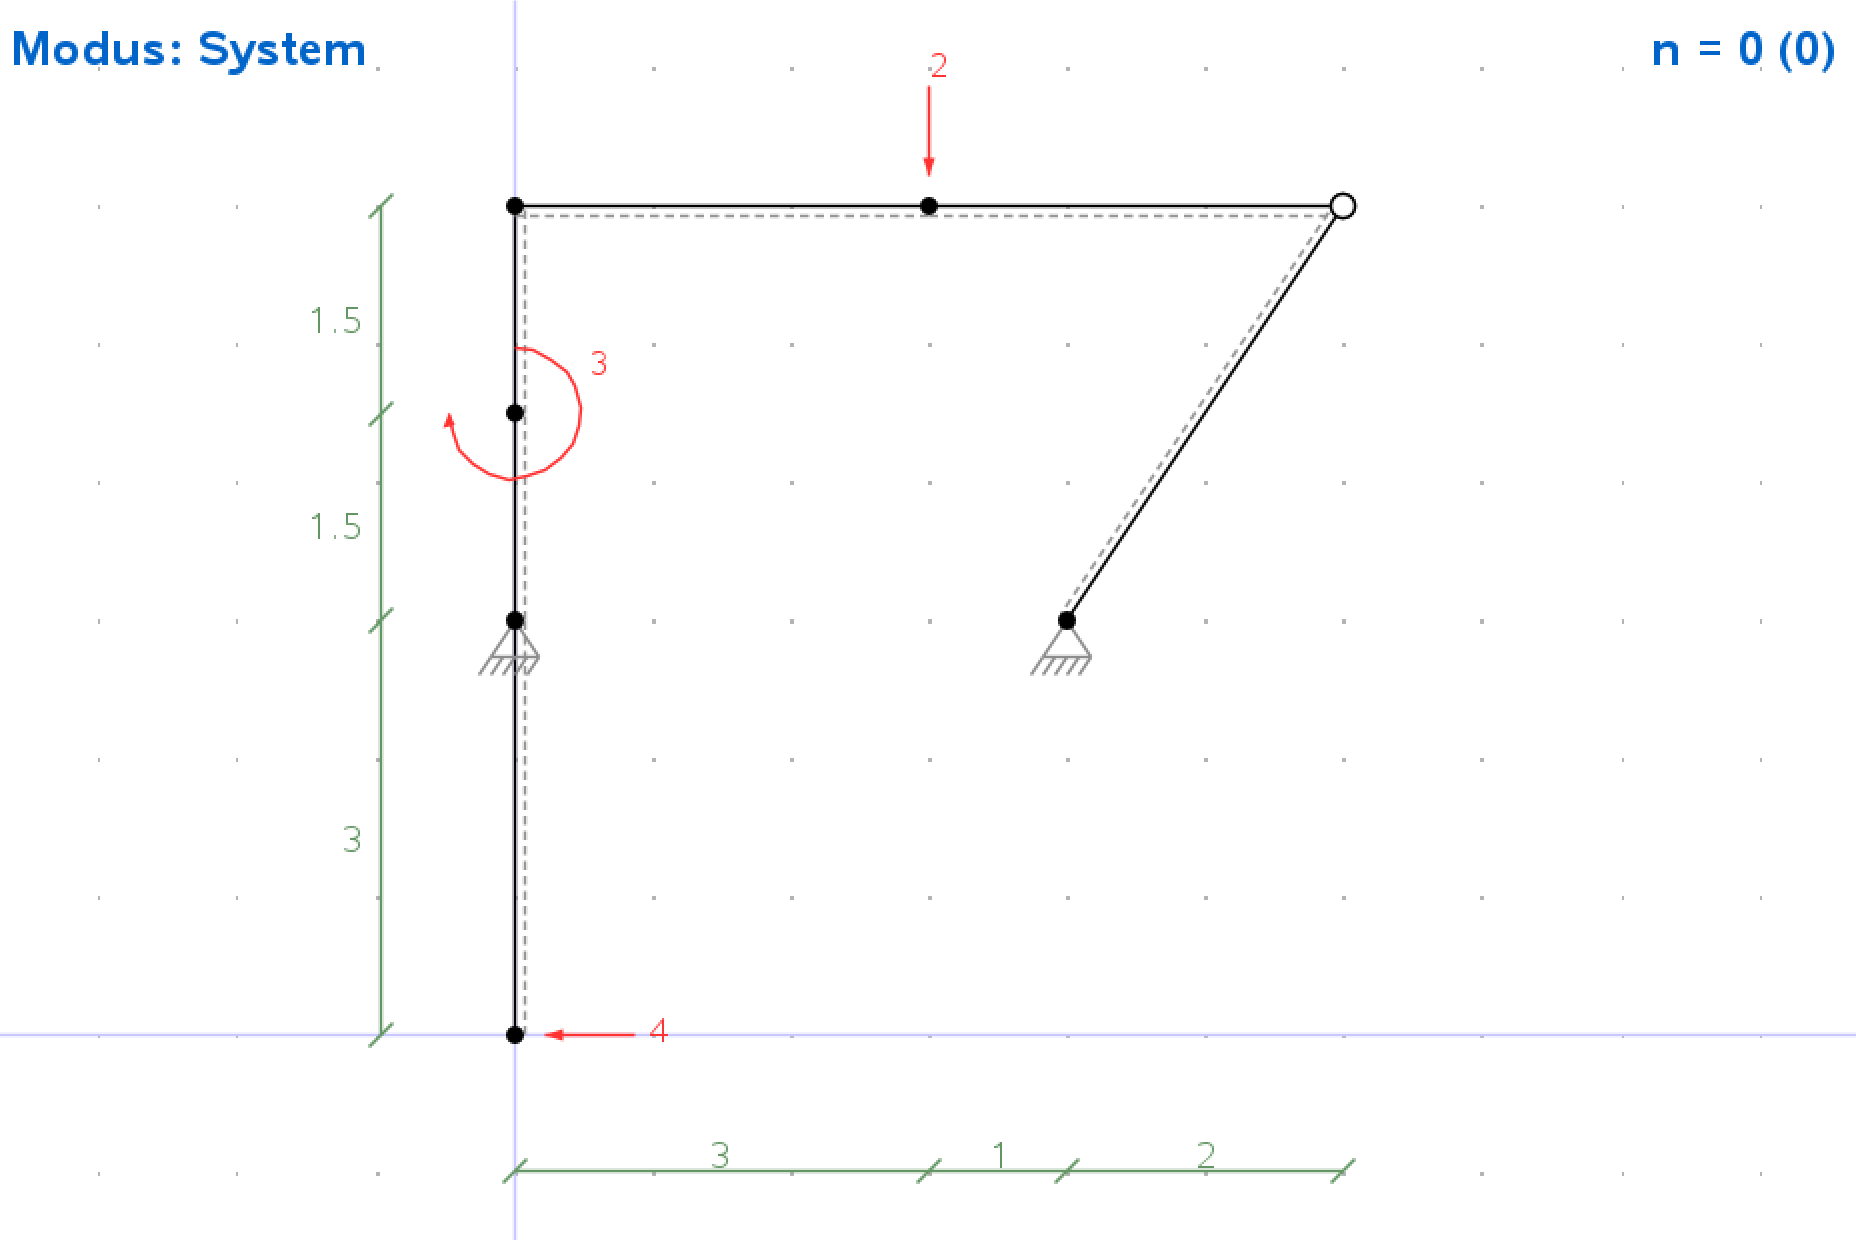
\includegraphics[width=0.5\linewidth]{./fig/TM1/WiSe2122nr3_1.png}
    \caption{TM1 WiSe~21/22, Nr.~3 im Programm}
    \label{fig:TM1WiSe2122Nr3_1}
\end{figure}

\begin{figure}[htbp]
    \centering
    \begin{subfigure}[t]{0.48\textwidth}
        \centering
        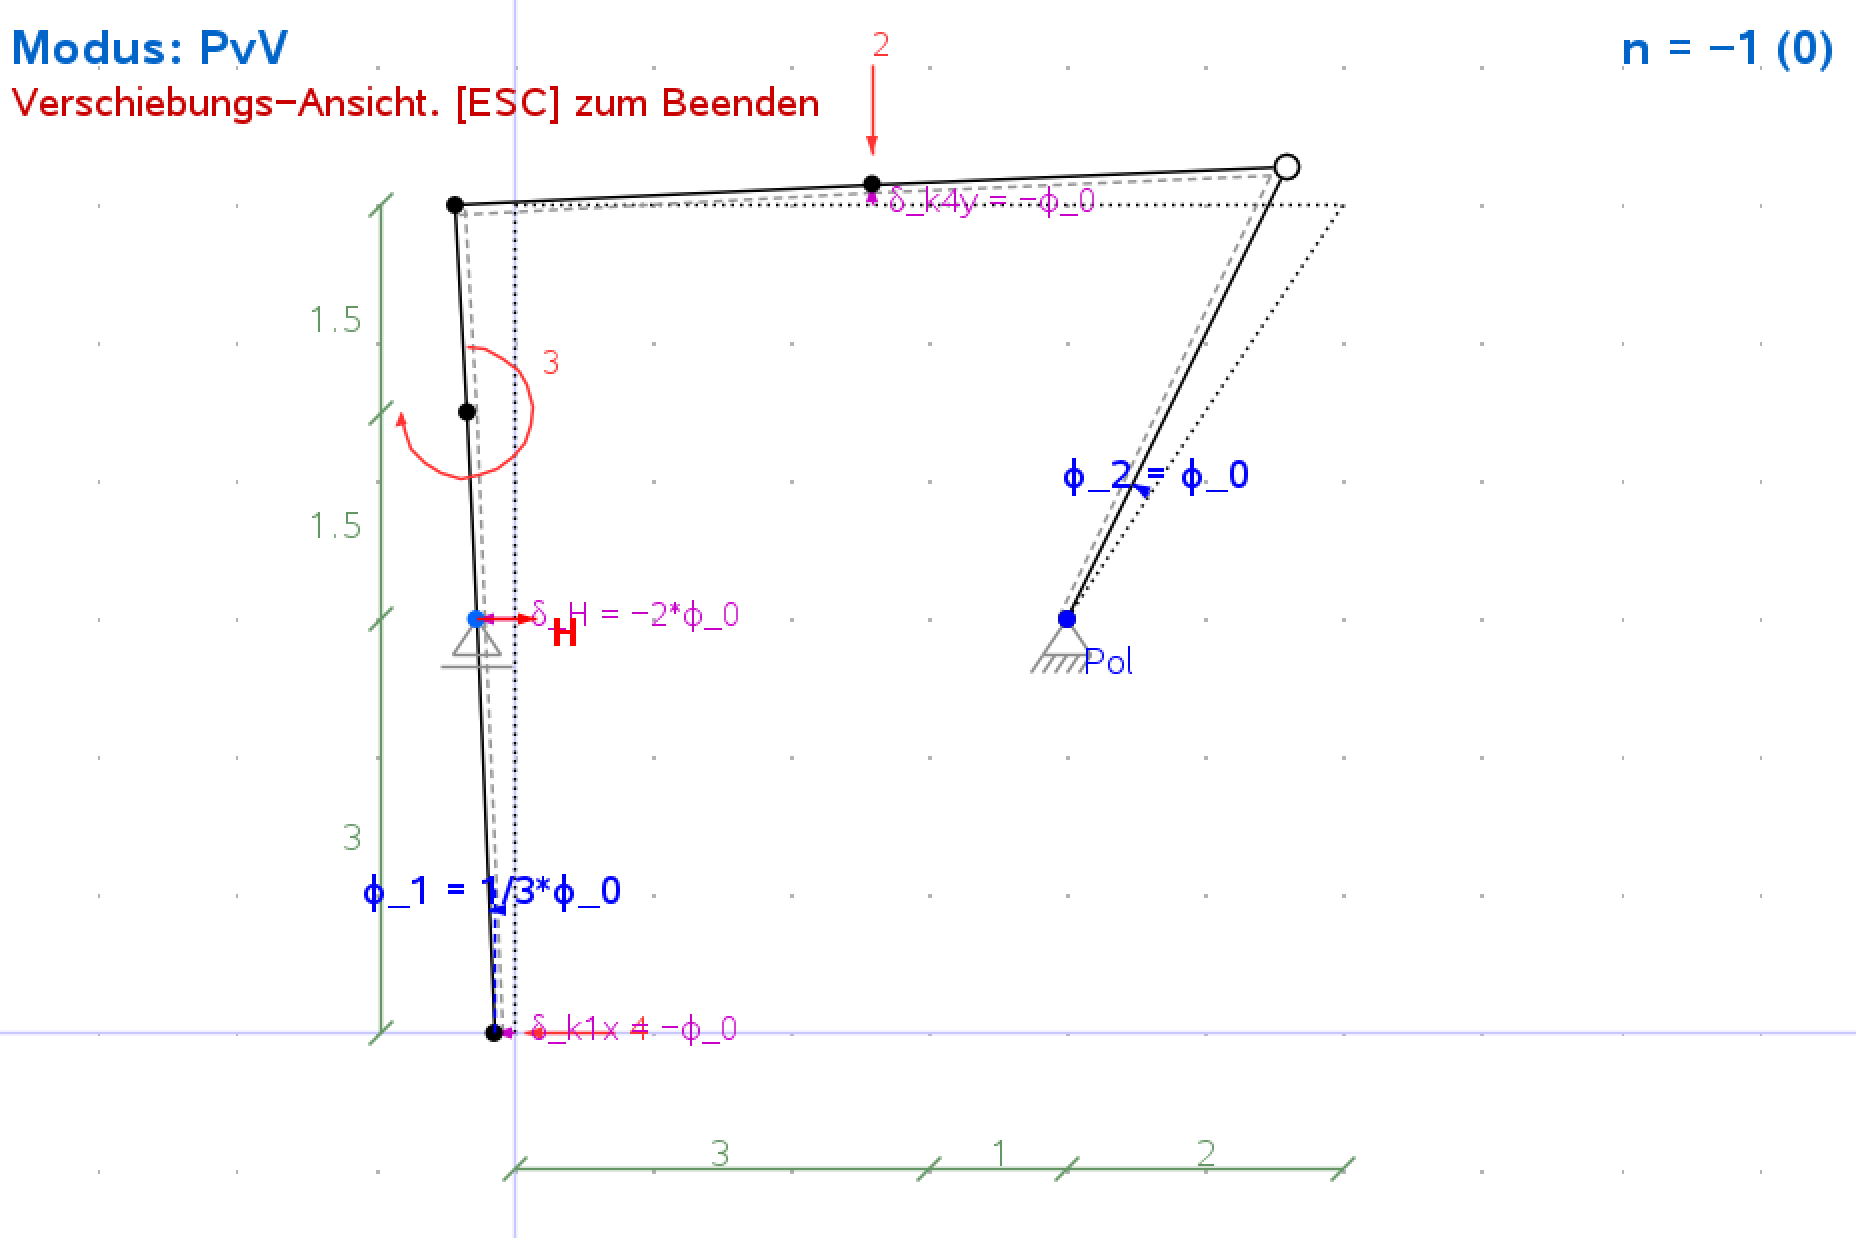
\includegraphics[width=\linewidth]{./fig/TM1/WiSe2122nr3_2.png}
        \caption{Verschiebungsfigur für $A_H$}
    \end{subfigure}
    \hfill
    \begin{subfigure}[t]{0.48\textwidth}
        \centering
        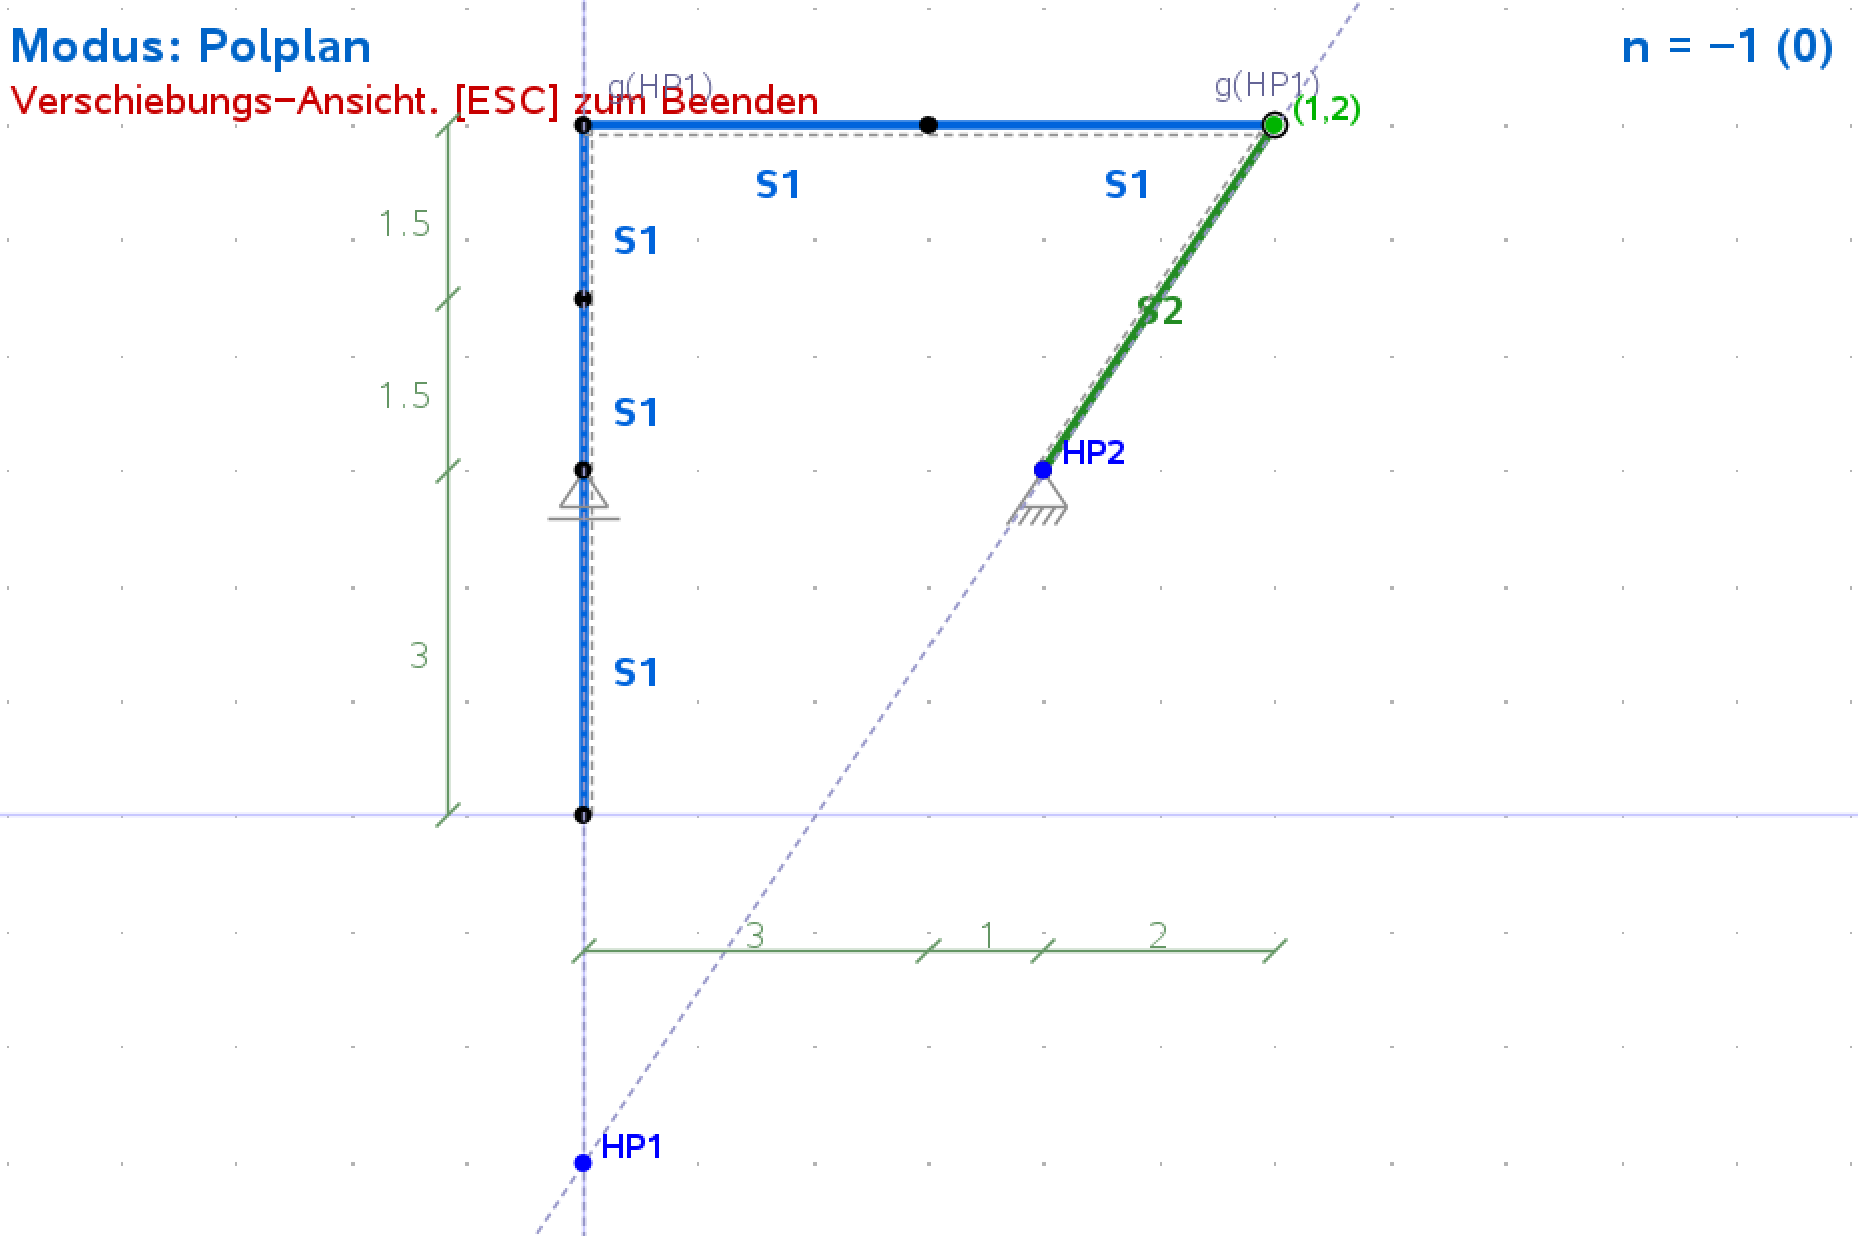
\includegraphics[width=\linewidth]{./fig/TM1/WiSe2122nr3_3.png}
        \caption{Polplan für $A_H$}
    \end{subfigure}
    \caption{WiSe~21/22, Nr.~3: $A_H$}
    \label{fig:TM1WiSe2122Nr3_2}
\end{figure}

\begin{figure}[htbp]
    \centering
    \begin{subfigure}[t]{0.48\textwidth}
        \centering
        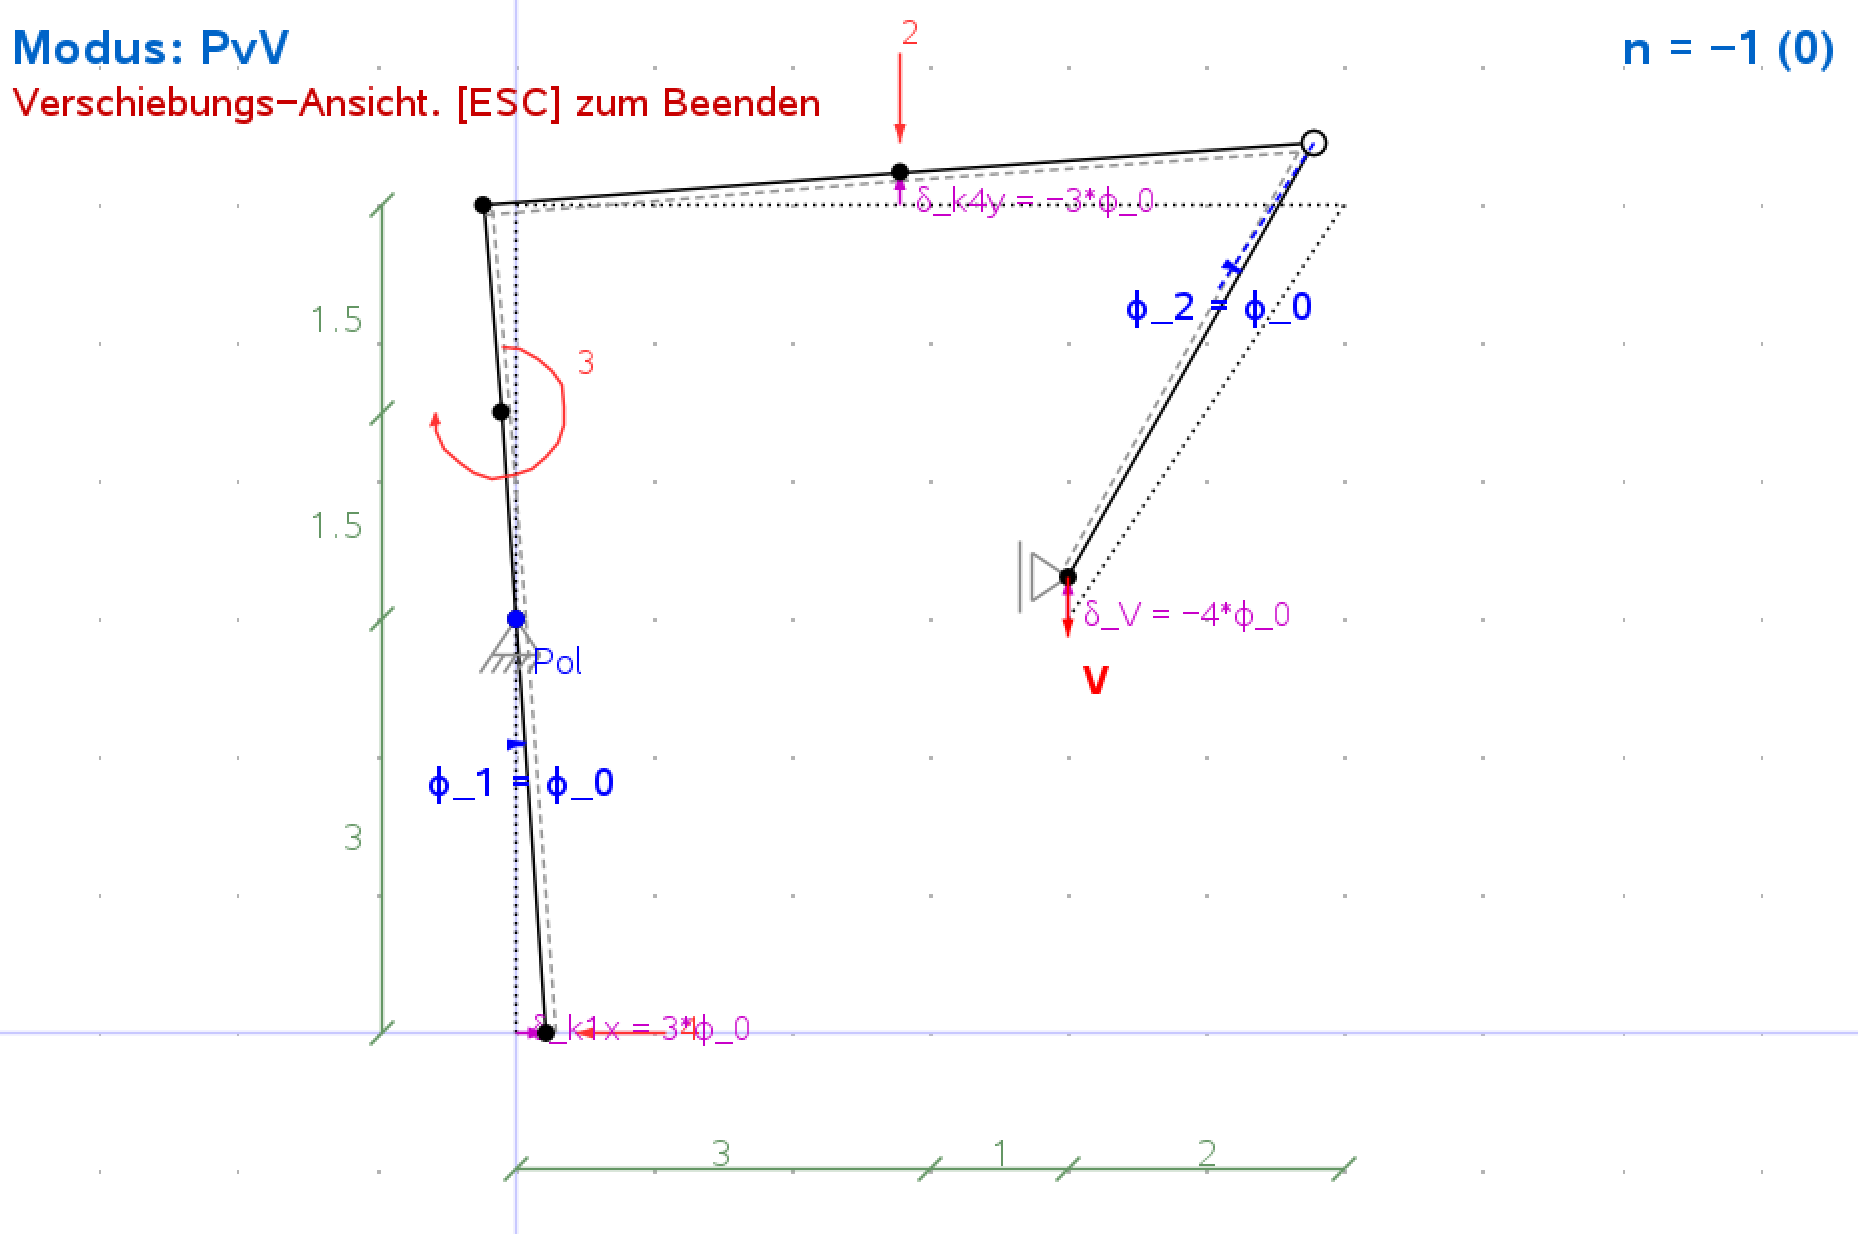
\includegraphics[width=\linewidth]{./fig/TM1/WiSe2122nr3_4.png}
        \caption{Verschiebungsfigur für $B_V$}
    \end{subfigure}
    \hfill
    \begin{subfigure}[t]{0.48\textwidth}
        \centering
        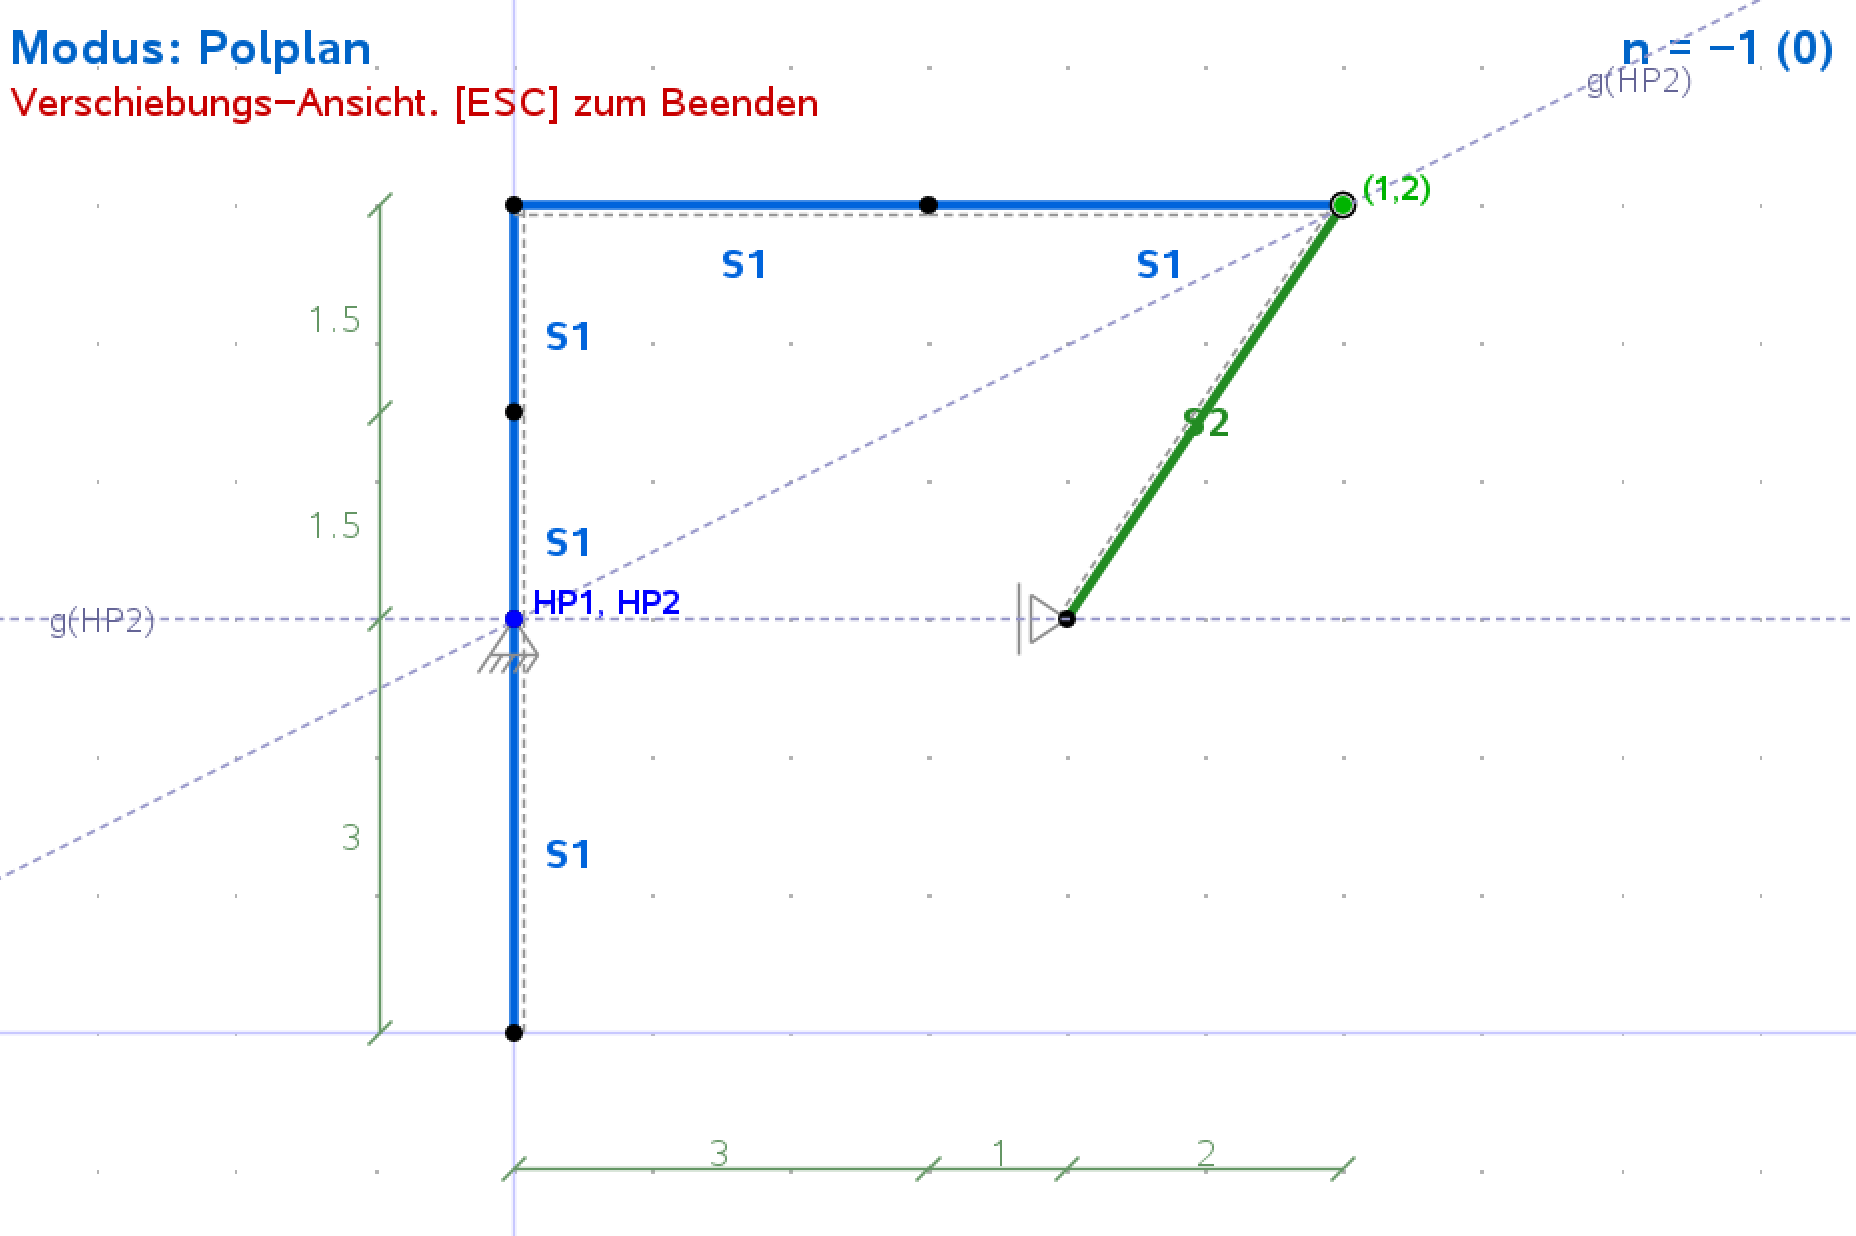
\includegraphics[width=\linewidth]{./fig/TM1/WiSe2122nr3_5.png}
        \caption{Polplan für $B_V$}
    \end{subfigure}
    \caption{WiSe~21/22, Nr.~3: $B_V$}
    \label{fig:TM1WiSe2122Nr3_3}
\end{figure}

Die Zeilen der Matrizen \code{pvv\_kin} und \code{pvv\_pol} (Abb.~\ref{fig:TM1WiSe2122Nr3_4})
sind als Gleichungskette zu lesen. Hier gilt also z.B. $\delta_{k1x}= -3\cdot\varphi_1=-\varphi_0$, oder 
$\delta x_{p12}= -9\cdot\varphi_1=-3\varphi_2$. Mit diesen Gleichungen lässt sich aus \code{w\_eq1} \code{w\_eq2} bauen.
Diese gleichung lässt sich dann entweder von hand oder mit dem Taschenrechner nach der gesuchten Größe auflösen.

\begin{figure}[htbp]
    \centering
    \begin{subfigure}[t]{0.48\textwidth}
        \centering
        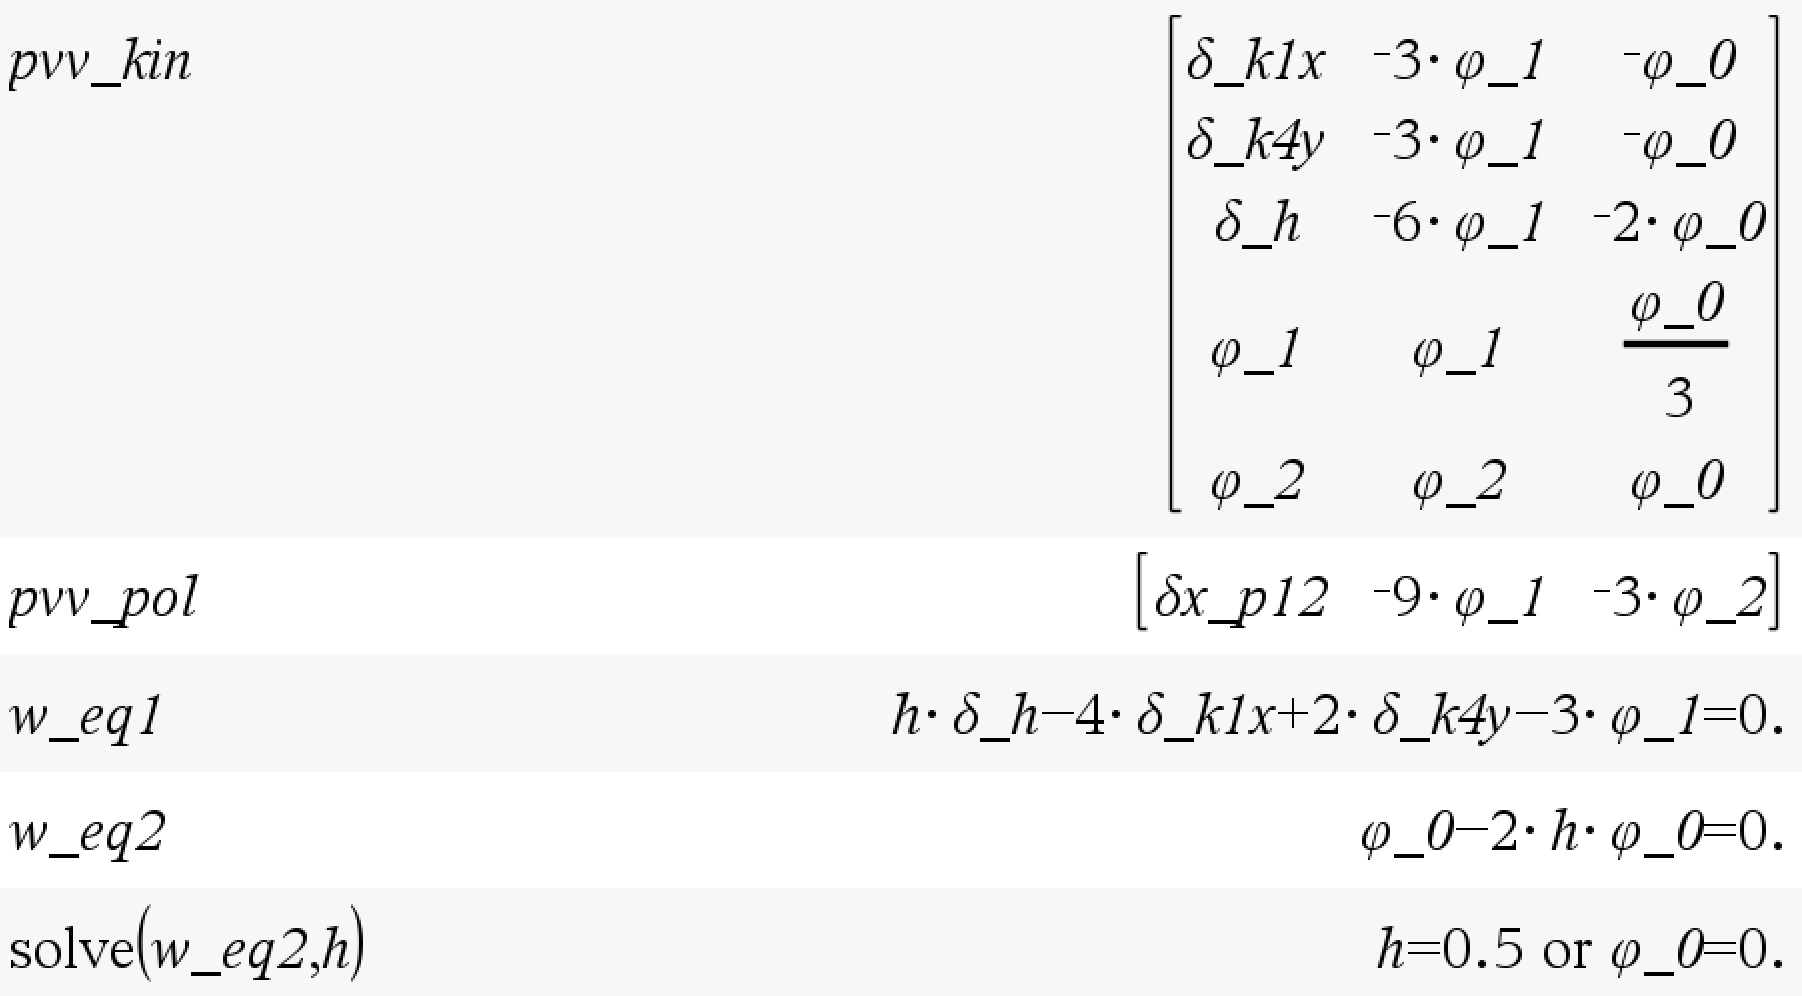
\includegraphics[width=\linewidth]{./fig/TM1/WiSe2122nr3_6.png}
        \caption{Rechnung für $A_H$}
    \end{subfigure}
    \hfill
    \begin{subfigure}[t]{0.48\textwidth}
        \centering
        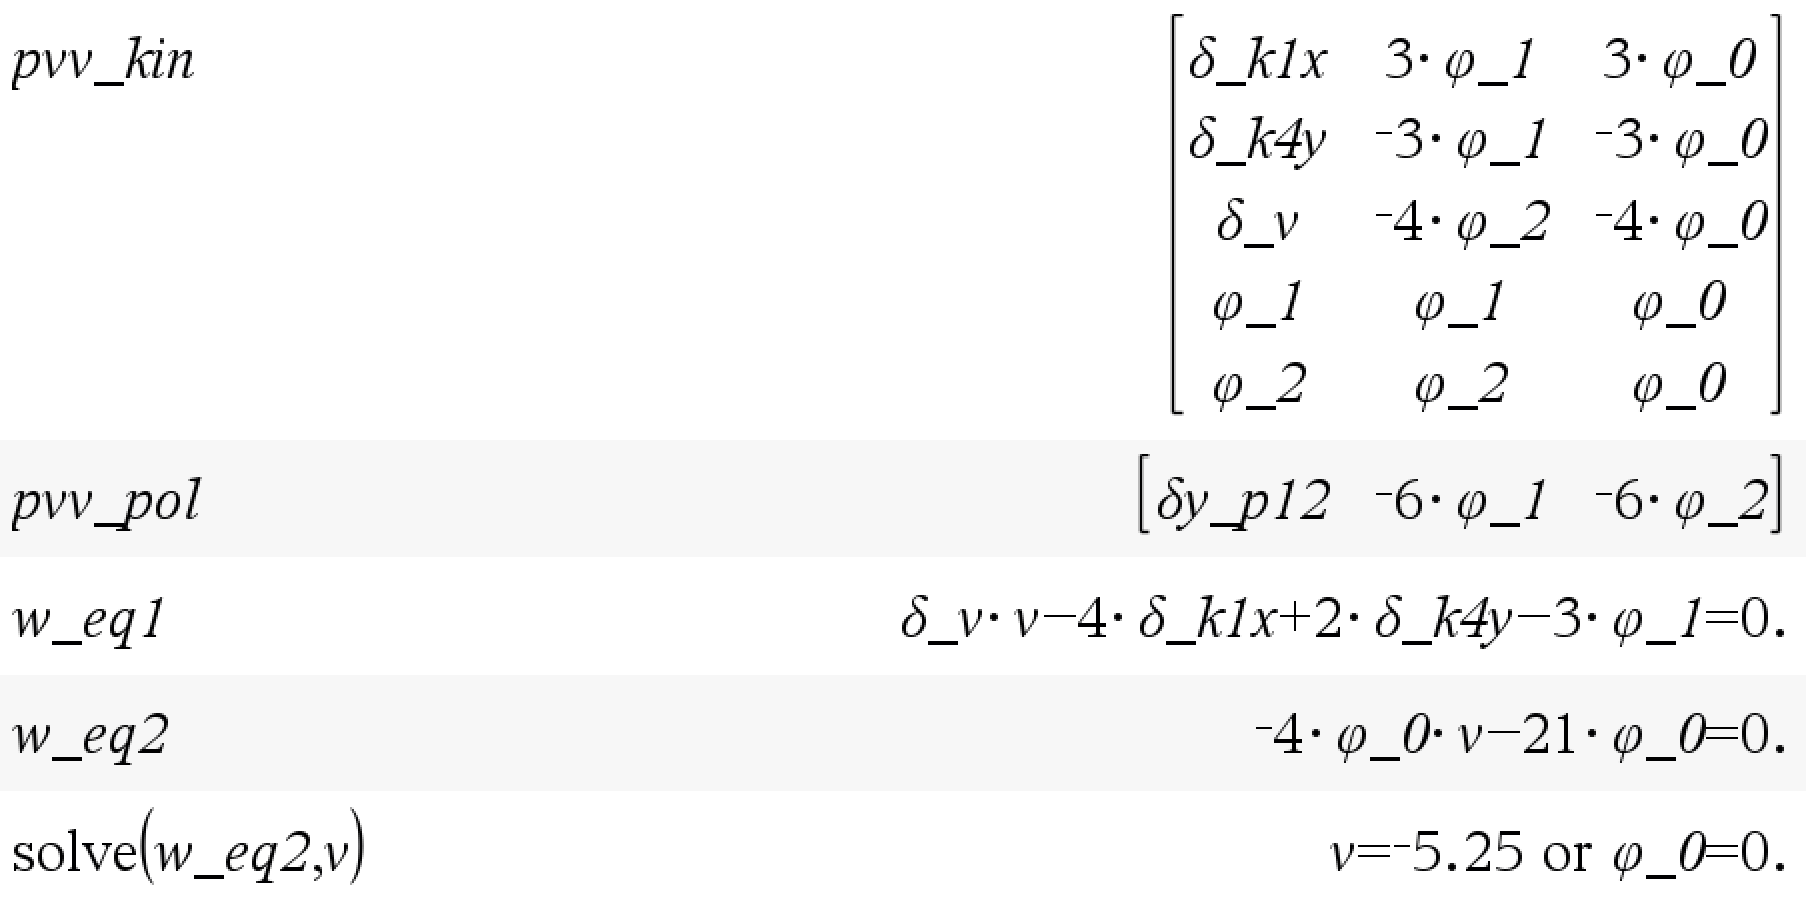
\includegraphics[width=\linewidth]{./fig/TM1/WiSe2122nr3_7.png}
        \caption{Rechnung für $B_V$}
    \end{subfigure}
    \caption{WiSe~21/22, Nr.~3: Ergebnis}
    \label{fig:TM1WiSe2122Nr3_4}
\end{figure}

\subsection{Schnittkräfte Bögen (Nr.~5)}

Mit dem Programm lassen sich die Funktionen für Schnittkraftverläufe von normalen Stäben als auch von Bögen 
ausgeben. Bei bögen ist die Laufvraibale nur nicht mehr die Länge entlang des Stabes sondern der Winkel.
also für diese Aufgabe zweilmal $\varphi \in [0,\frac{\pi}{4}]$ bzw. $\varphi \in [0,90\text{°}]$. Hier ist die Winkel-Einstellung
des Taschenrechenrs wichtig.\\
Hier gilt aber auch wieder, dass das Programm das nicht wirklich so ausrechnet wie man das von Hand machen würde, sondern
es sucht eine schöne Darstellung der Anfangswerte und kombiniert diese dann zur Funktion.

\begin{figure}[htbp]
    \centering
    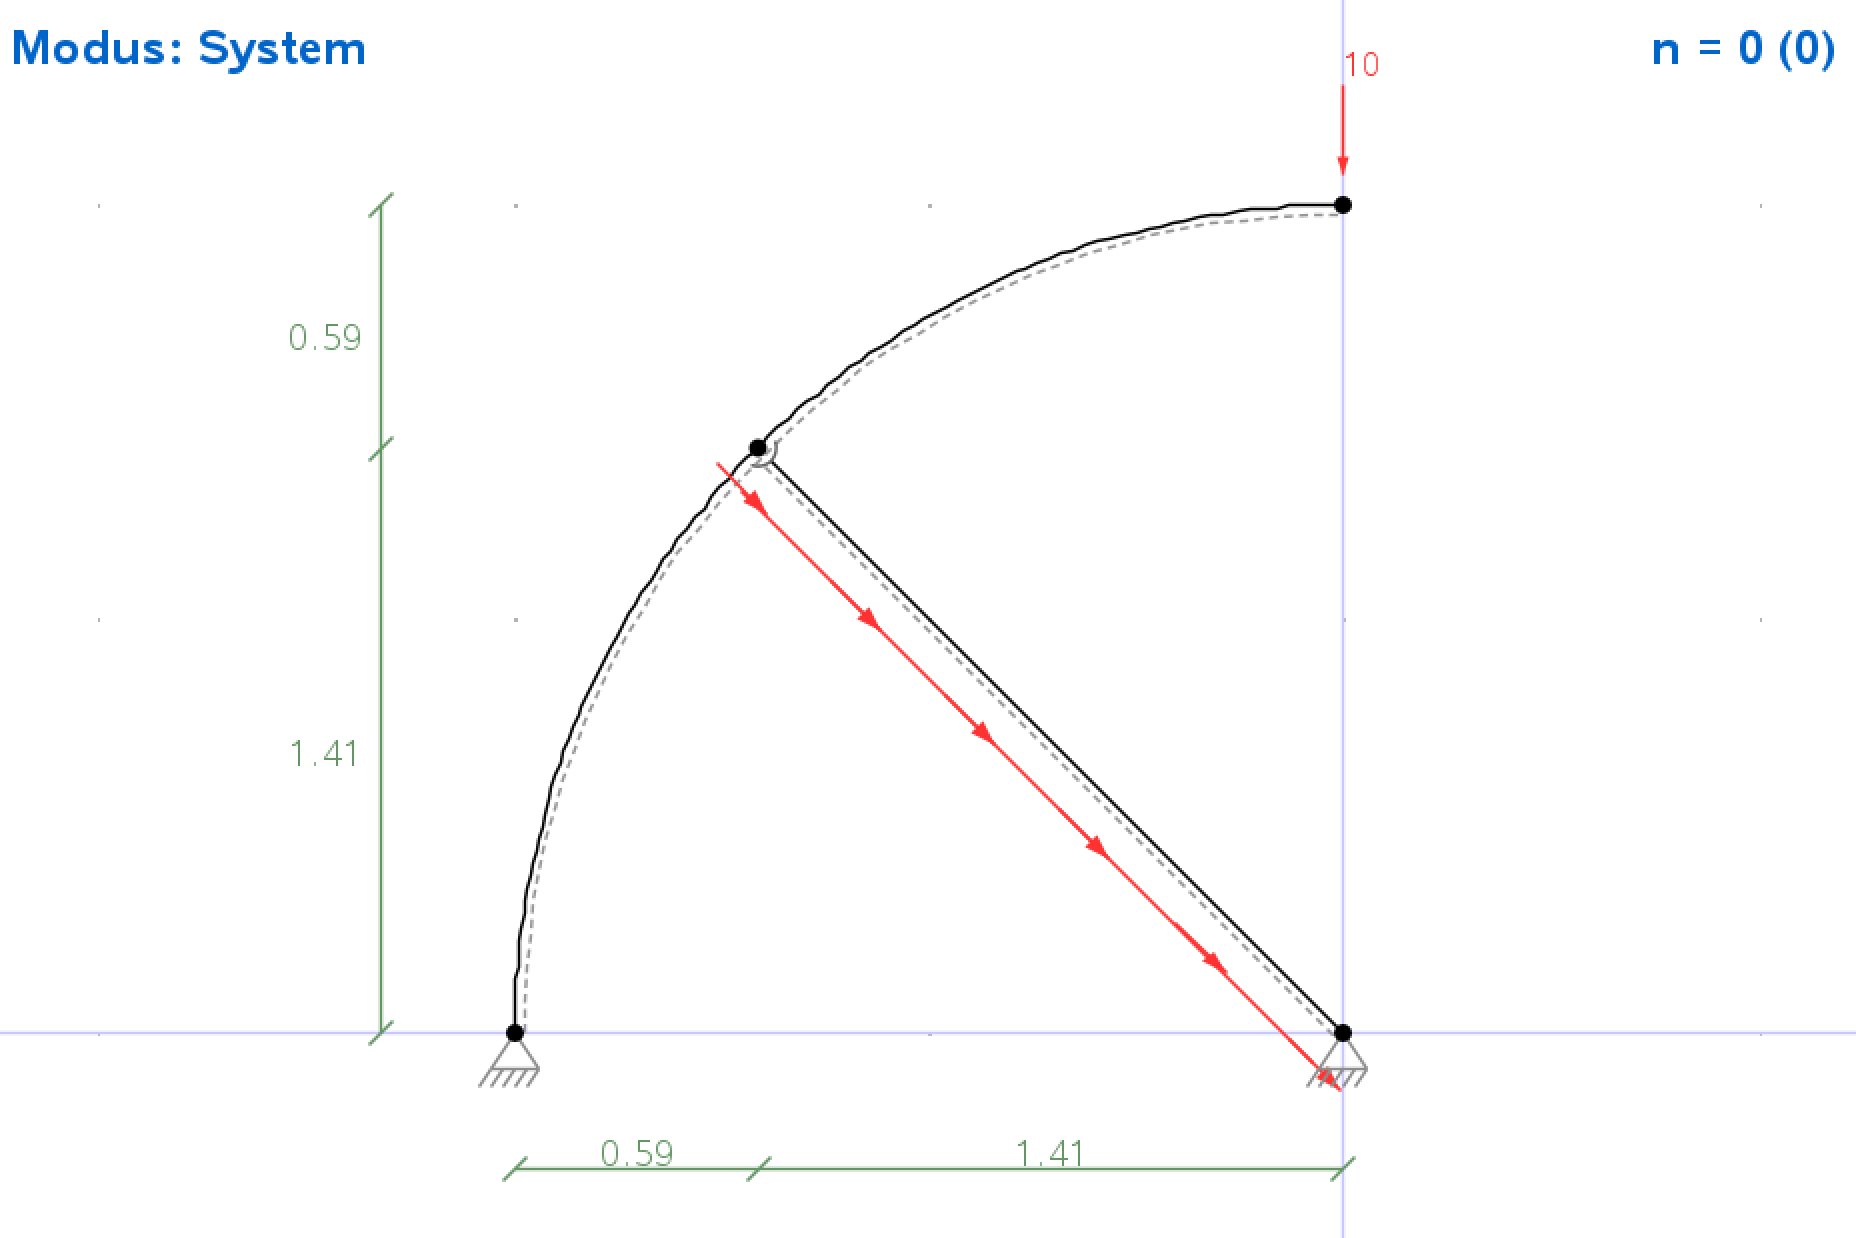
\includegraphics[width=0.5\linewidth]{./fig/TM1/WiSe2122nr5_1.png}
    \caption{TM1 WiSe~21/22, Nr.~5 im Programm}
    \label{fig:TM1WiSe2122Nr5_1}
\end{figure}


\subsection{Fachwerk (Nr.6)}

Vom Prinzip werden Fachwerke genau gleich eingegeben wie normale Systeme, nur das hier die orientierung der gestrichelten Faser
keine Rolle spielt. Es ist jedoch sinnvoll den Fachwerk Modus anzumachen, dann wird die statische Bestimmtheit beim hovern über $n=$ 
auch die Formel für Fachwerke verwendet und alle Knoten werden zu vollgelenken gemacht, auch wenn der Modus erst nach dem 
zeichnen des Systems angemacht wird.  


\begin{figure}[htbp]
    \centering
    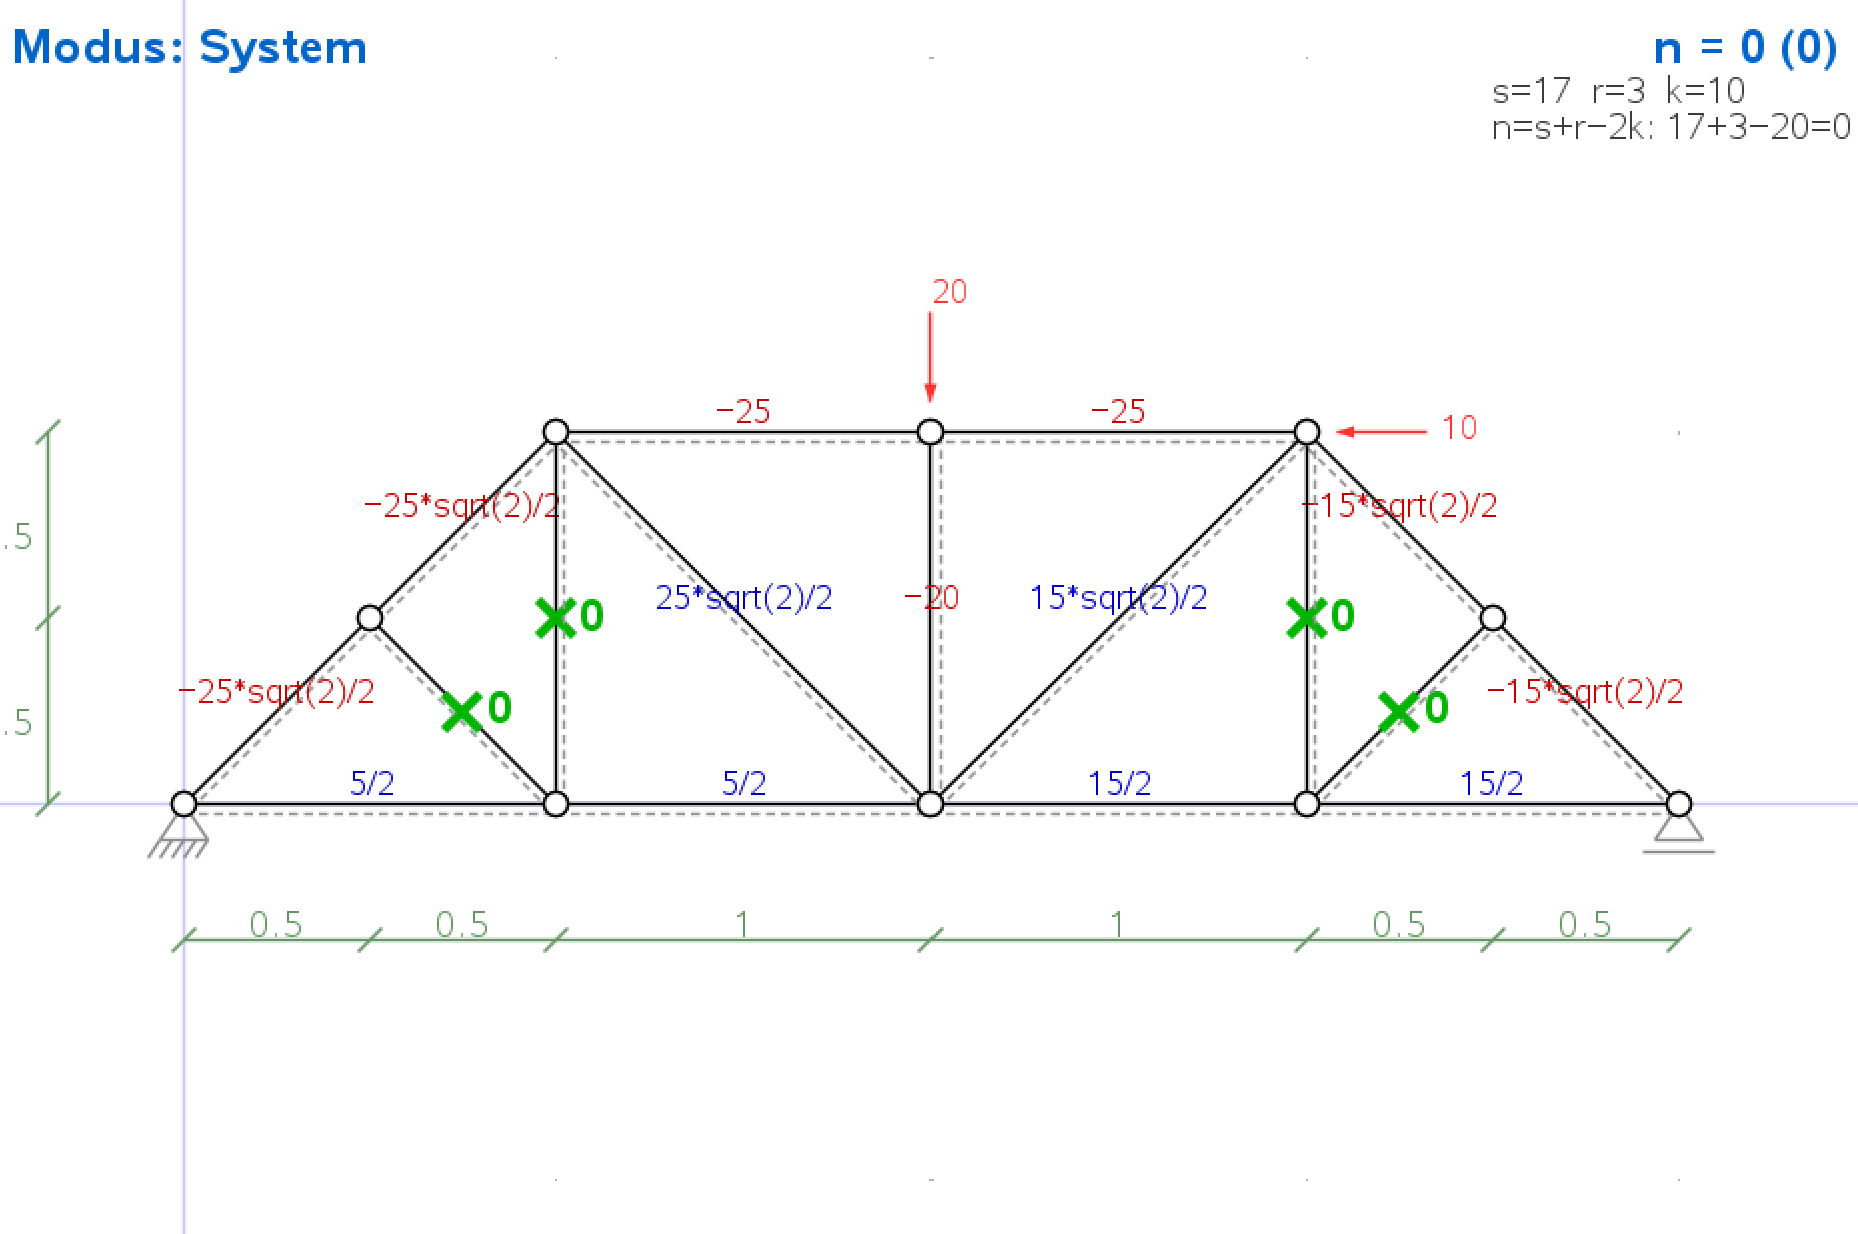
\includegraphics[width=0.5\linewidth]{./fig/TM1/WiSe2122nr6_1.png}
    \caption{TM1 WiSe~21/22, Nr.~6 im Programm}
    \label{fig:TM1WiSe2122Nr6_1}
\end{figure}

Die Stabe in Abb.~\ref{fig:TM1WiSe2122Nr6_1} die ein grünes Kreuz haben sind die ohne Rechnung erkennbaren Nullstäbe
Falls nach der Berechnung stäbkkräfte mit einer grünen Null beschriftet werdsen, aber dort kein Kreuz ist, ist das zwar ein 
Nullstab der aber nicht direkt aus den Regeln erkennbar ist. Für Afgaben bei denen nach Nullstäben gefragt wird, also nur 
die durchgekreuzten Stäbe angeben

\begin{figure}[htbp]
    \centering
    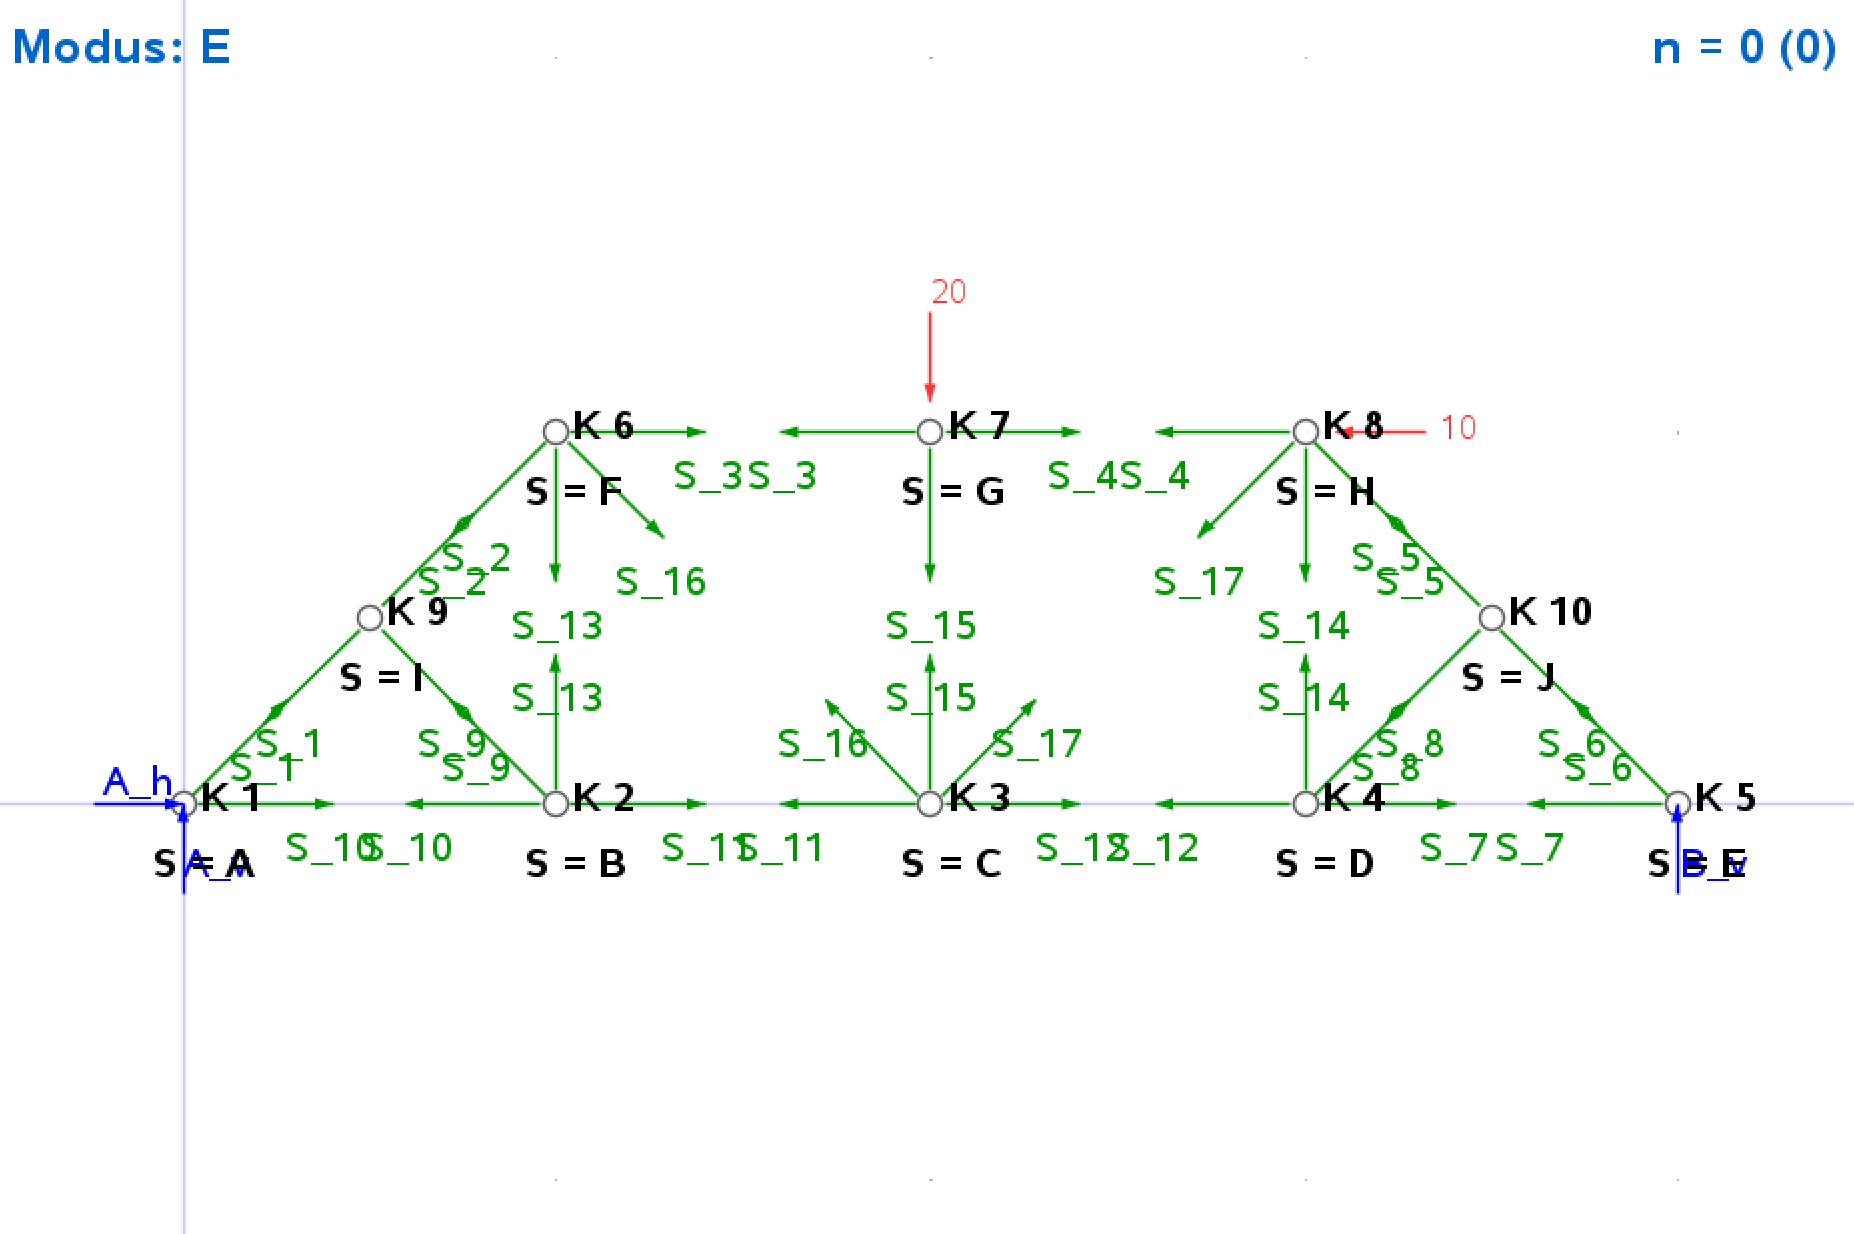
\includegraphics[width=0.5\linewidth]{./fig/TM1/WiSe2122nr6_2.png}
    \caption{TM1 WiSe~21/22 Freischnitt}
    \label{fig:TM1WiSe2122Nr6_2}
\end{figure}

Für die Verwendung der beiden Seiten des E-Modus muss darauf geachtet werden, dass entweder die Stäbe in der
gleichen Reihenfolge wie in der Aufgabe gezeichnet werden oder die Bennenung hinterher angepasst wird. Macht ihr das nicht
ist z.B. Stab 13 aus eurer Rechnung nicht Stab 13 aus der Aufgabe\\
Gleiches gilt natürlich auch für die Verwendung des LGS-Exports. Hier wird (Falls der Fachwerk Modus an ist) 
das Knotenschnittverfahren verwendet. Die Benennung im LGS ist die gleiche wie auf der zweiten Seite des E-Modus.





\section{TM2}

\subsection{Biegelinie (TM2 WiSe~21/22, Nr.~7)} \label{ex:Biegelinienaufgabe}

In dieser Aufgabe ist ein \emph{interessantes} KOS vorgegeben: Soll es ein Rechtssystem sein,
zeigt die $y$-Achse hier in die Zeichenebene hinein und nicht, wie sonst üblich, aus ihr heraus.

Rechnet ihr von Hand über die DGL $EI\,w'''' = q$ mit allen Rand- und Übergangsbedingungen (so
geht man bei statisch unbestimmten Systemen meist vor, und so rechnet auch \code{wneu}), gibt es
hier nichts weiter zu beachten. Bei einem statisch bestimmten System lohnt es sich dagegen, zuerst
die Momentenlinie zu berechnen und dann $EI\,w'' = -M$ zu integrieren. Dafür braucht ihr die
gestrichelte Faser. Die Regel aus Abschnitt~\ref{sec:Eingabe_Stäbe}, dass sie immer auf der Seite
liegt, in die die $z$- bzw.\ $w$-Achse zeigt, gilt auch hier. Alternativ könnt ihr euch überlegen,
auf welcher Seite ein positives Schnittmoment $M_y$ (Drehsinn nach der Rechte-Hand-Regel um die
$y$-Achse) Zug erzeugt, dort liegt die gestrichelte Faser. Das finde ich aber umständlicher.

Im Programm müsst ihr solche Systeme etwas anders eingeben, denn dort zeigt die $y$-Achse immer
aus der Zeichenebene heraus. Zeichnet ihr das System genau wie in der Aufgabe und setzt die
gestrichelte Faser nach der Regel oben, läuft die $x$-Koordinate im Programm in die andere Richtung
als in der Aufgabe. Um das zu umgehen, zeichnet ihr Systeme, bei denen die $y$-Achse in die
Zeichenebene hineinzeigt, spiegelverkehrt (Abb.~\ref{fig:Biegelinienaufgabe}). Ich habe die
Aufgabe im symbolischen Modus gerechnet, deshalb stehen in den Ergebnissen $q$ und $l$.

\begin{figure}[htbp]
    \centering
    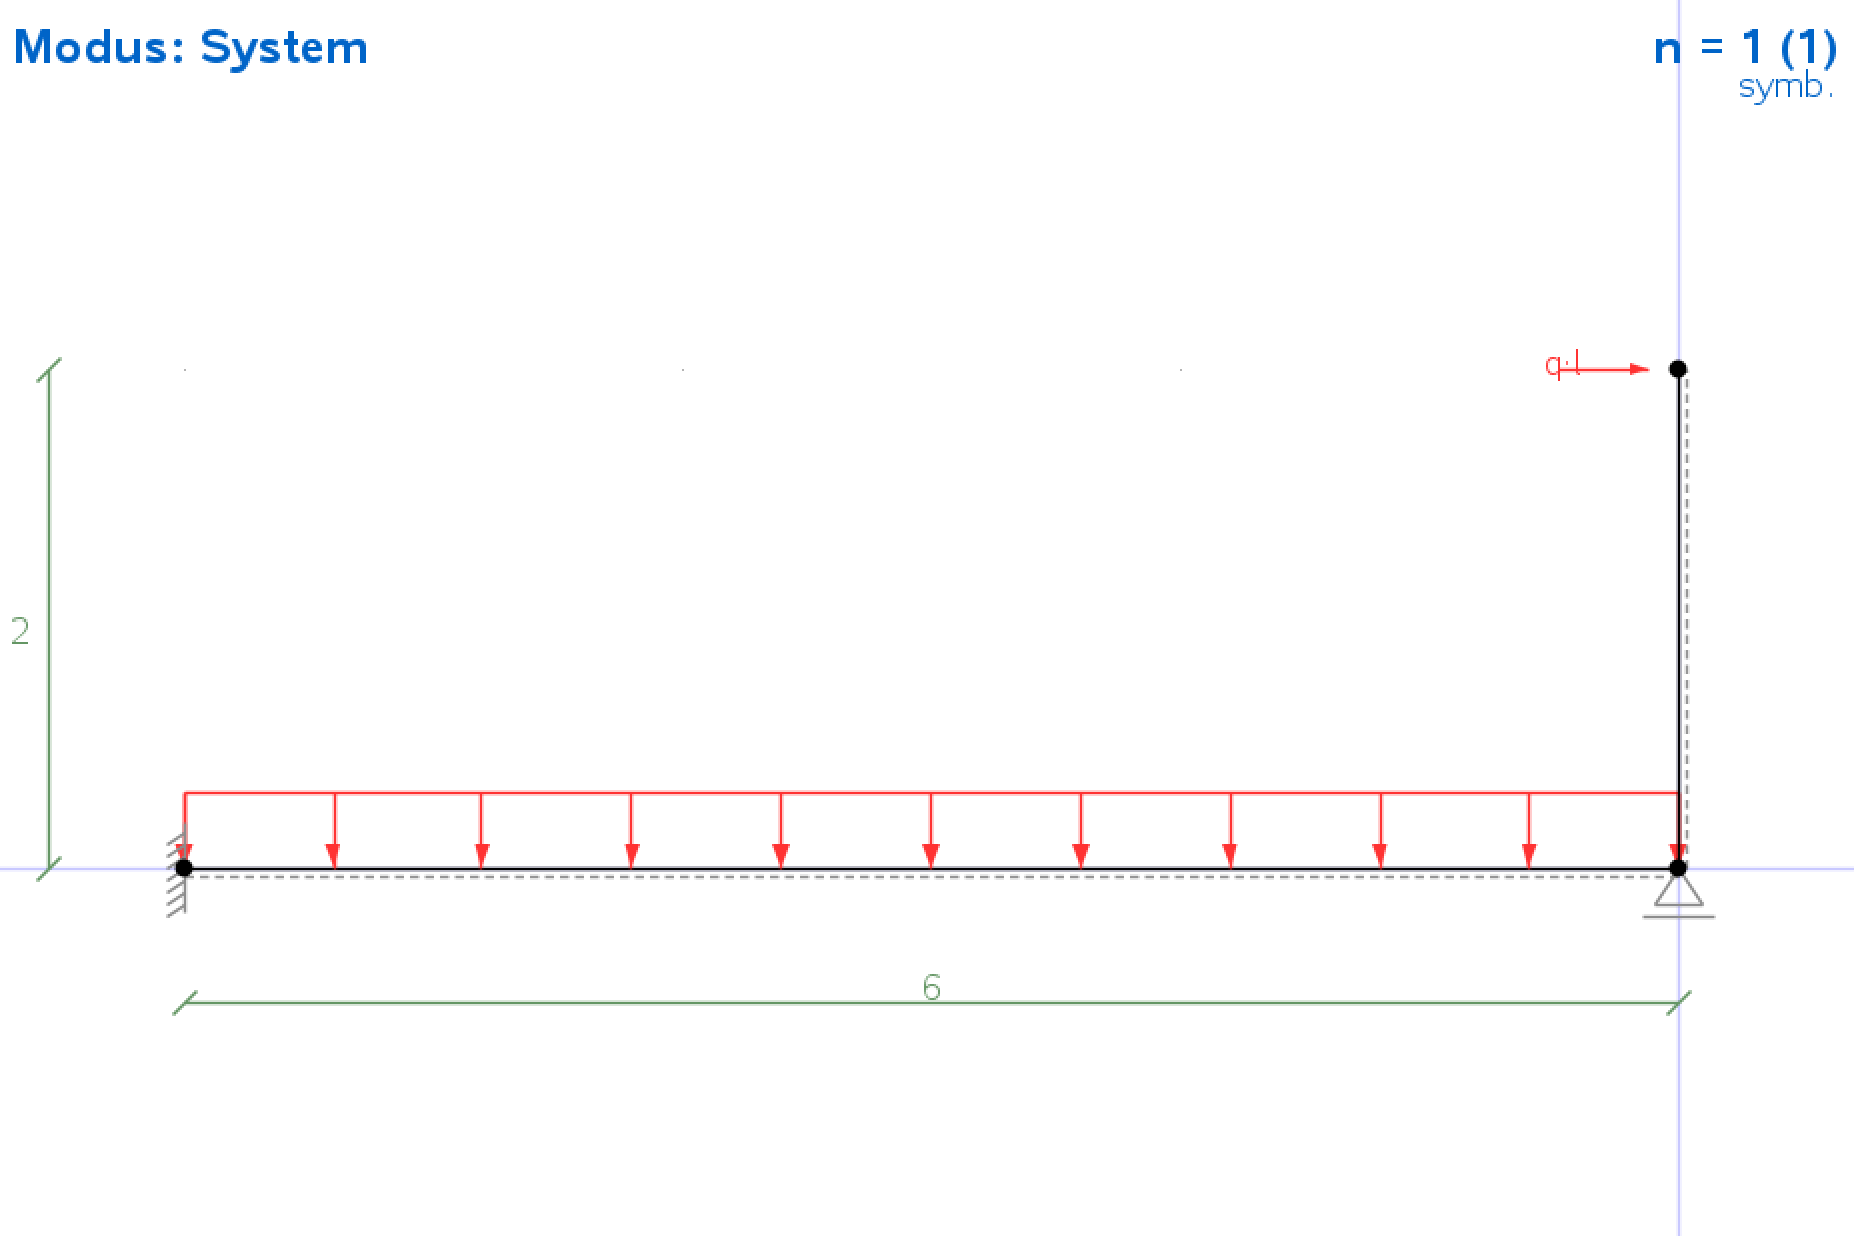
\includegraphics[width=0.5\linewidth]{./fig/TM2/WiSe2122nr7_1.png}
    \caption{TM2 WiSe~21/22, Nr.~7 im Programm, spiegelverkehrt gezeichnet}
    \label{fig:Biegelinienaufgabe}
\end{figure}

Das liefert die Ergebnisse in Abb.~\ref{fig:BiegelinienaufgabeBiegelinie}. Hier geben beide
Methoden dasselbe Ergebnis. Das sollte natürlich so sein, ist aber nicht immer so: Manchmal weicht
die WGV/FEM-Lösung \code{v\_EI\_stab1(x)} (im Rechner klein geschrieben) minimal von der exakten
Lösung \code{wneu1(x)} ab. Weil das Programm die Brüche aus den Zahlen der FEM-Lösung
\emph{errät} (Abschnitt~\ref{sec:mathe-symbolisch}), kann daraus eine ganz anders aussehende
Biegelinie werden. Die Methode über die WGV/FEM-Lösung gibt es trotzdem, vor allem weil ich sie
zuerst programmiert habe (daher wohl auch der Name \code{wneu} der anderen Funktion), und weil sie
bei sehr großen Systemen deutlich schneller sein kann.

\begin{figure}[htbp]
    \centering
    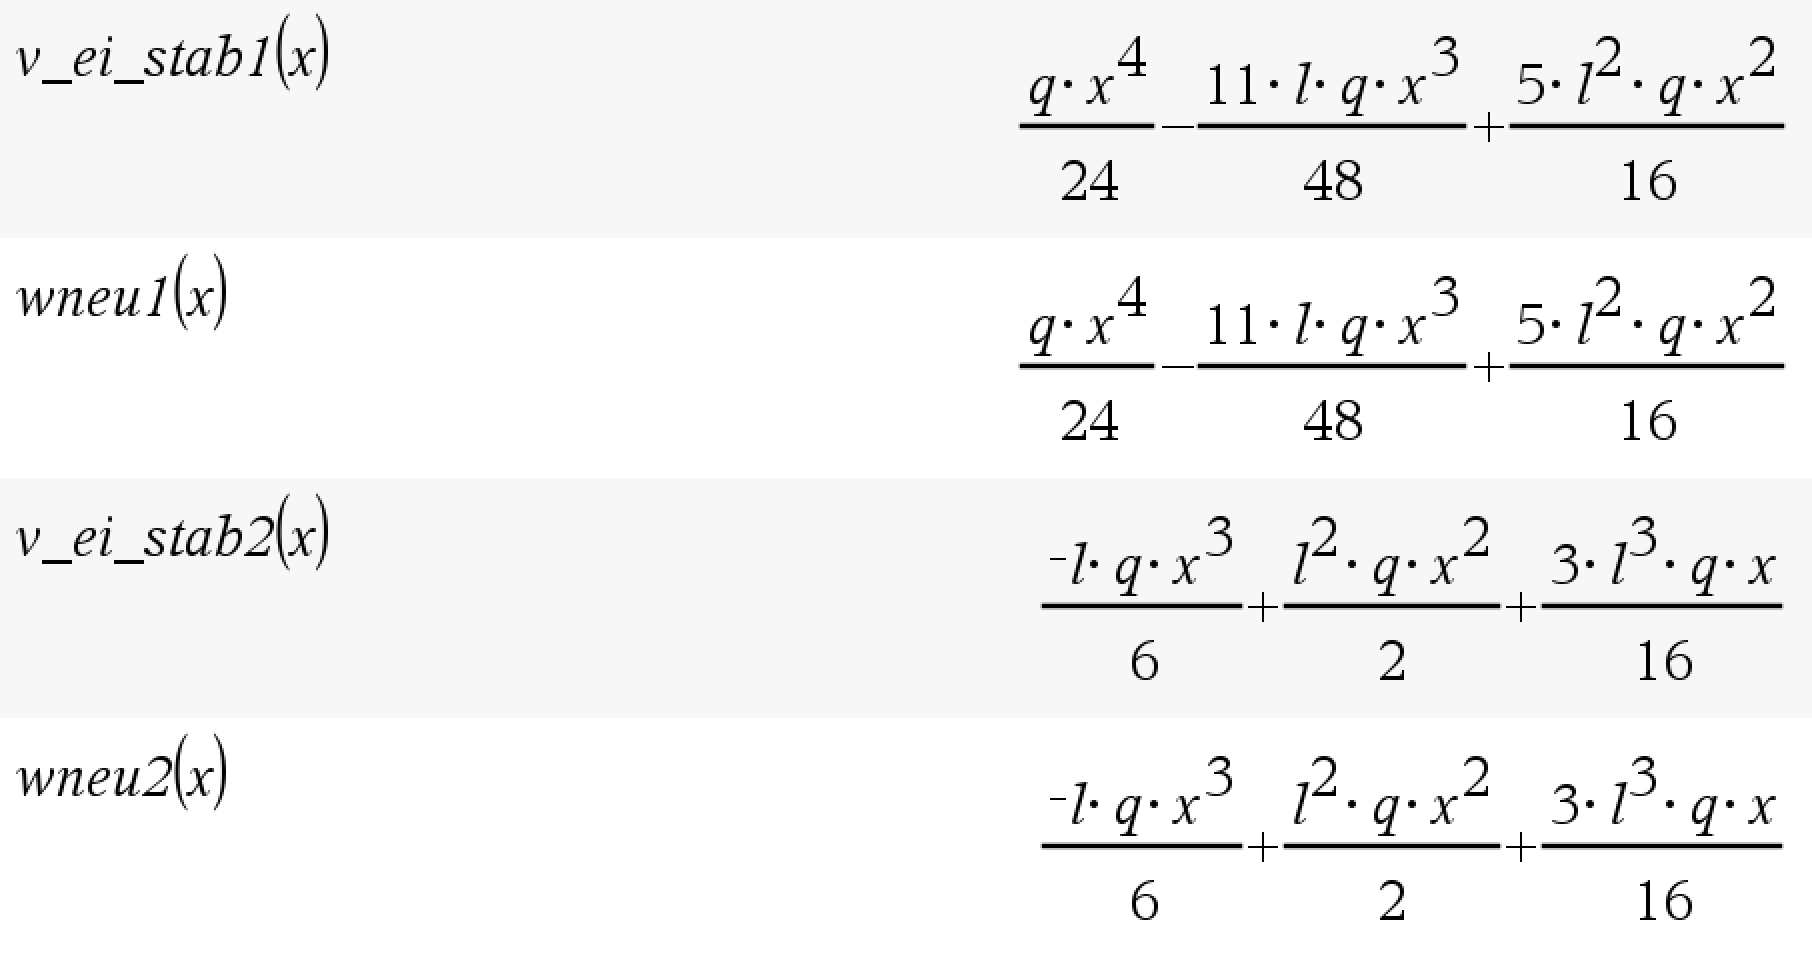
\includegraphics[width=0.5\linewidth]{./fig/TM2/WiSe2122nr7_2.png}
    \caption{TM2 WiSe~21/22, Nr.~7: \code{v\_EI\_stab} und \code{wneu} im Vergleich}
    \label{fig:BiegelinienaufgabeBiegelinie}
\end{figure}

Weil die Stäbe dehnsteif sind, kann das Programm hier sogar die Randbedingungen für Biegelinie und
Längslinie getrennt angeben (Abb.~\ref{fig:BiegelinienaufgabeRandbed}): Die Bedingungen im oberen
Block reichen für die Biegelinie allein, die im unteren kommen nur für die Längslinie dazu. Das geht
nicht immer. Sind die Stäbe dehnbar, hängt die Biegelinie über die Rahmenecken auch von den
Längsverformungen ab, und das Programm gibt alle Bedingungen zusammen aus
(Abschnitt~\ref{sec:randlgs}).

\begin{figure}[htbp]
    \centering
    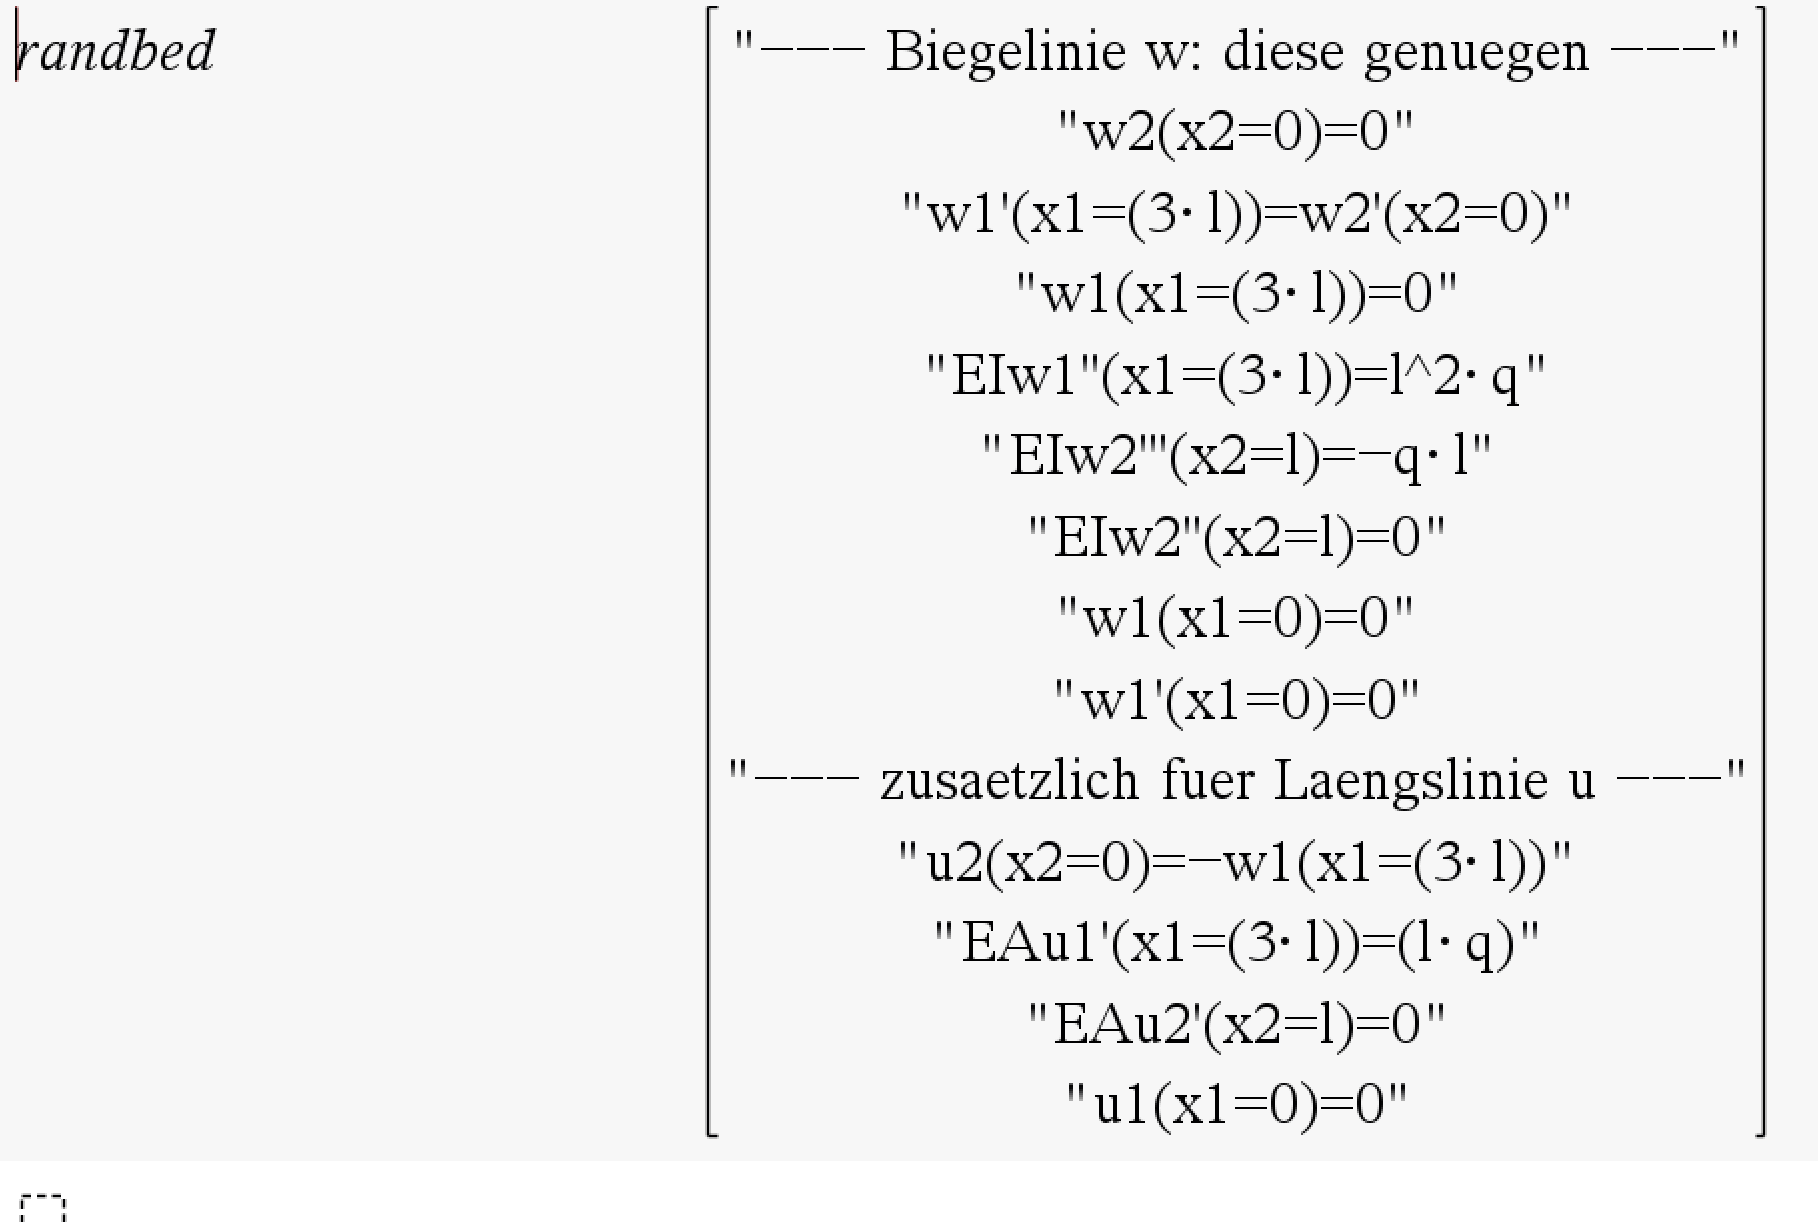
\includegraphics[width=0.5\linewidth]{./fig/TM2/WiSe2122nr7_3.png}
    \caption{Randbedingungen \code{randbed} für TM2 WiSe~21/22, Nr.~7}
    \label{fig:BiegelinienaufgabeRandbed}
\end{figure}



\subsection{Verschiebungsaufgaben (TM2 WiSe~20/21 Nr.~4)} \label{ex:Temperaturaufgabe}

Aufgaben wie diese lassen sich mit der richtigen Eingabe auch direkt im Programm lösen. Wie diese Aufagbe im
Programm aussieht ist in Abb.~\ref{fig:verschiebungSystem} dargestellt. Hierbei muss natürlich auf die Einheiten geachtet werden.
In der Aufgabe sind die relevanten Dehnsteifigkeiten nicht direkt gegeben, genauso wie manche Angaben nicht in der
für das Programm geforderten Einheit sind.\\
Für Kräfte immer kN, genauso wie für die Dehnsteifigkeit $EA$ und die Biegesteifigkeit $EI$ in kNm.  

\begin{figure}[htbp]
    \centering
    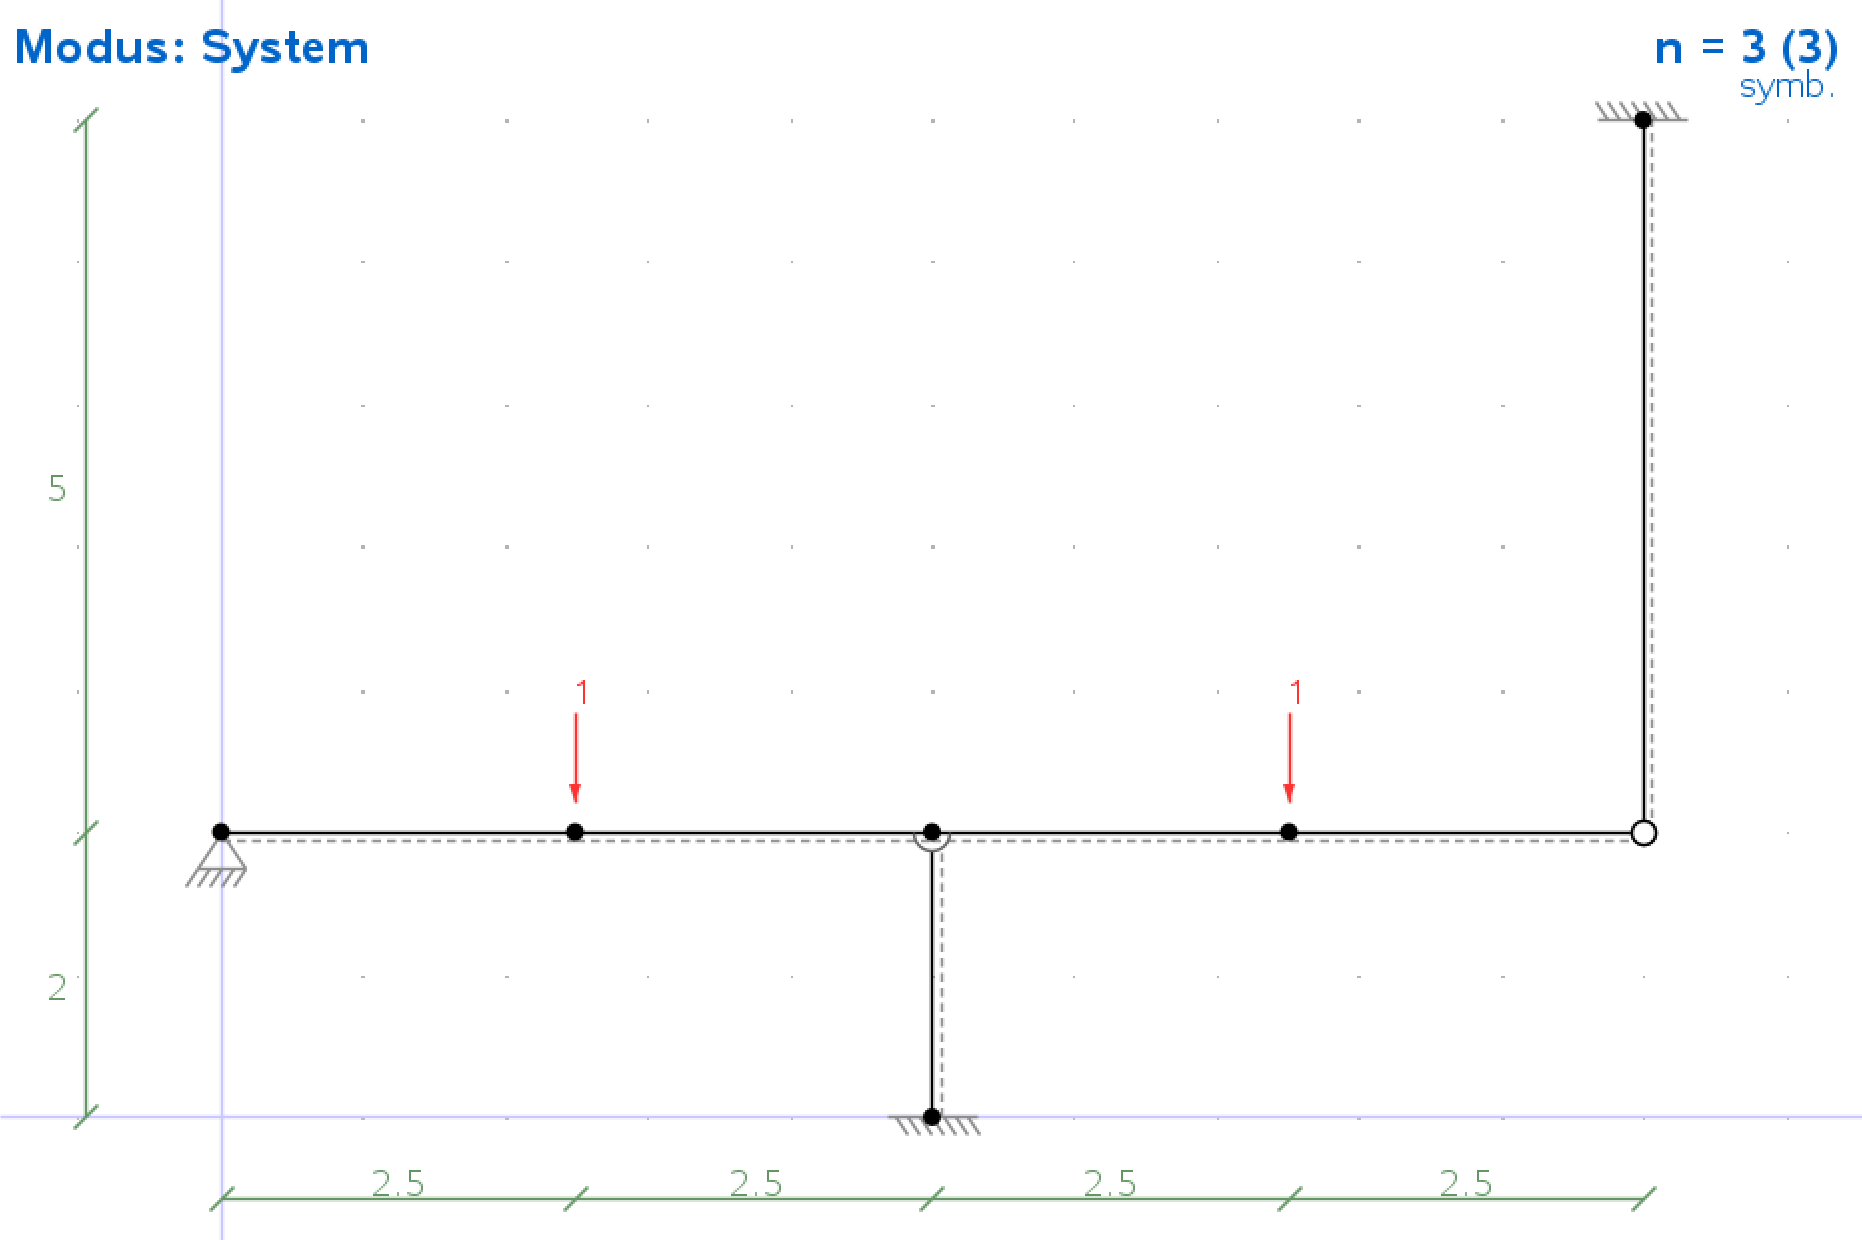
\includegraphics[width=0.5\linewidth]{./fig/TM2/WiSe2021nr4_1.png}
    \caption{TM2 WiSe~20/21, Nr.~4a im Programm}
    \label{fig:verschiebungSystem}
\end{figure}

In den \emph{neuen} Exportfunktionen wird die Temperatur auch symbolisch miteinberechnet.
Um also ann die Verschiebung des rechten unteren Knoten zu kommen lässt sich das entweder über die obere
Knotenexportfunktion machen, über die Biegelinie des rechten horizontalen Stabes oder über die Längsverschiebungsfunktion
des rechten vertikalen Stabes. Über den CAS Befehl \code{solve()} lässt sich die Temperatur direkt ausrechnen 
(vgl. Abb.~\ref{fig:verschiebungErgebniss}). Ich habe hier die Tempertur $dt$ genant (nur $T$ ist wie bereits erwähnt nicht erlaubt),
die Variable nach der aufgelöst werden soll muss der \code{solve()} Funktion als zweites Argument mit gegeben werden.

\begin{figure}[htbp]
    \centering
    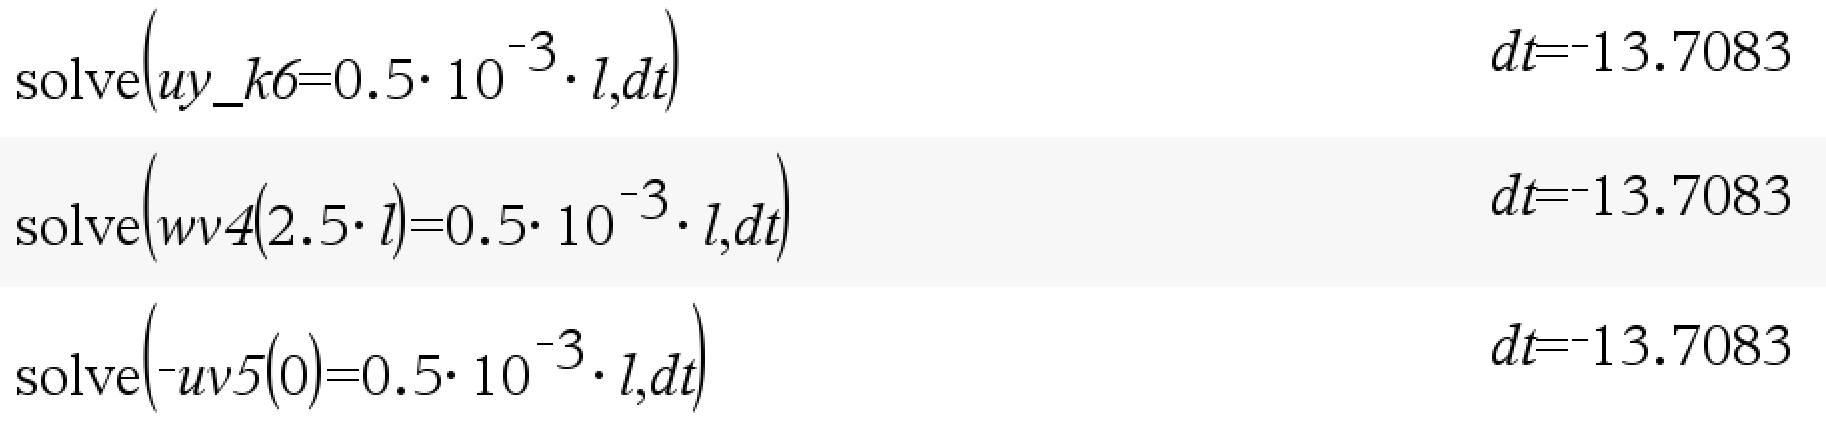
\includegraphics[width=0.5\linewidth]{./fig/TM2/WiSe2021nr4_2.png}
    \caption{Lösung von TM2 WiSe~20/21, Nr.~4a}
    \label{fig:verschiebungErgebniss}
\end{figure}

Der Zweite Teil der Aufgabe lässt sich auch im Programm lösen (Abb.~\ref{fig:VerschiebungTemp}), jedoch gibt es auch hier
ein paar Feinheiten. Ein deratiges System zu speichern kann sich lohnen. Auch hier gelten natürlich die gleichen Hinweise zu den Einheiten.

\begin{figure}[htbp]
    \centering
    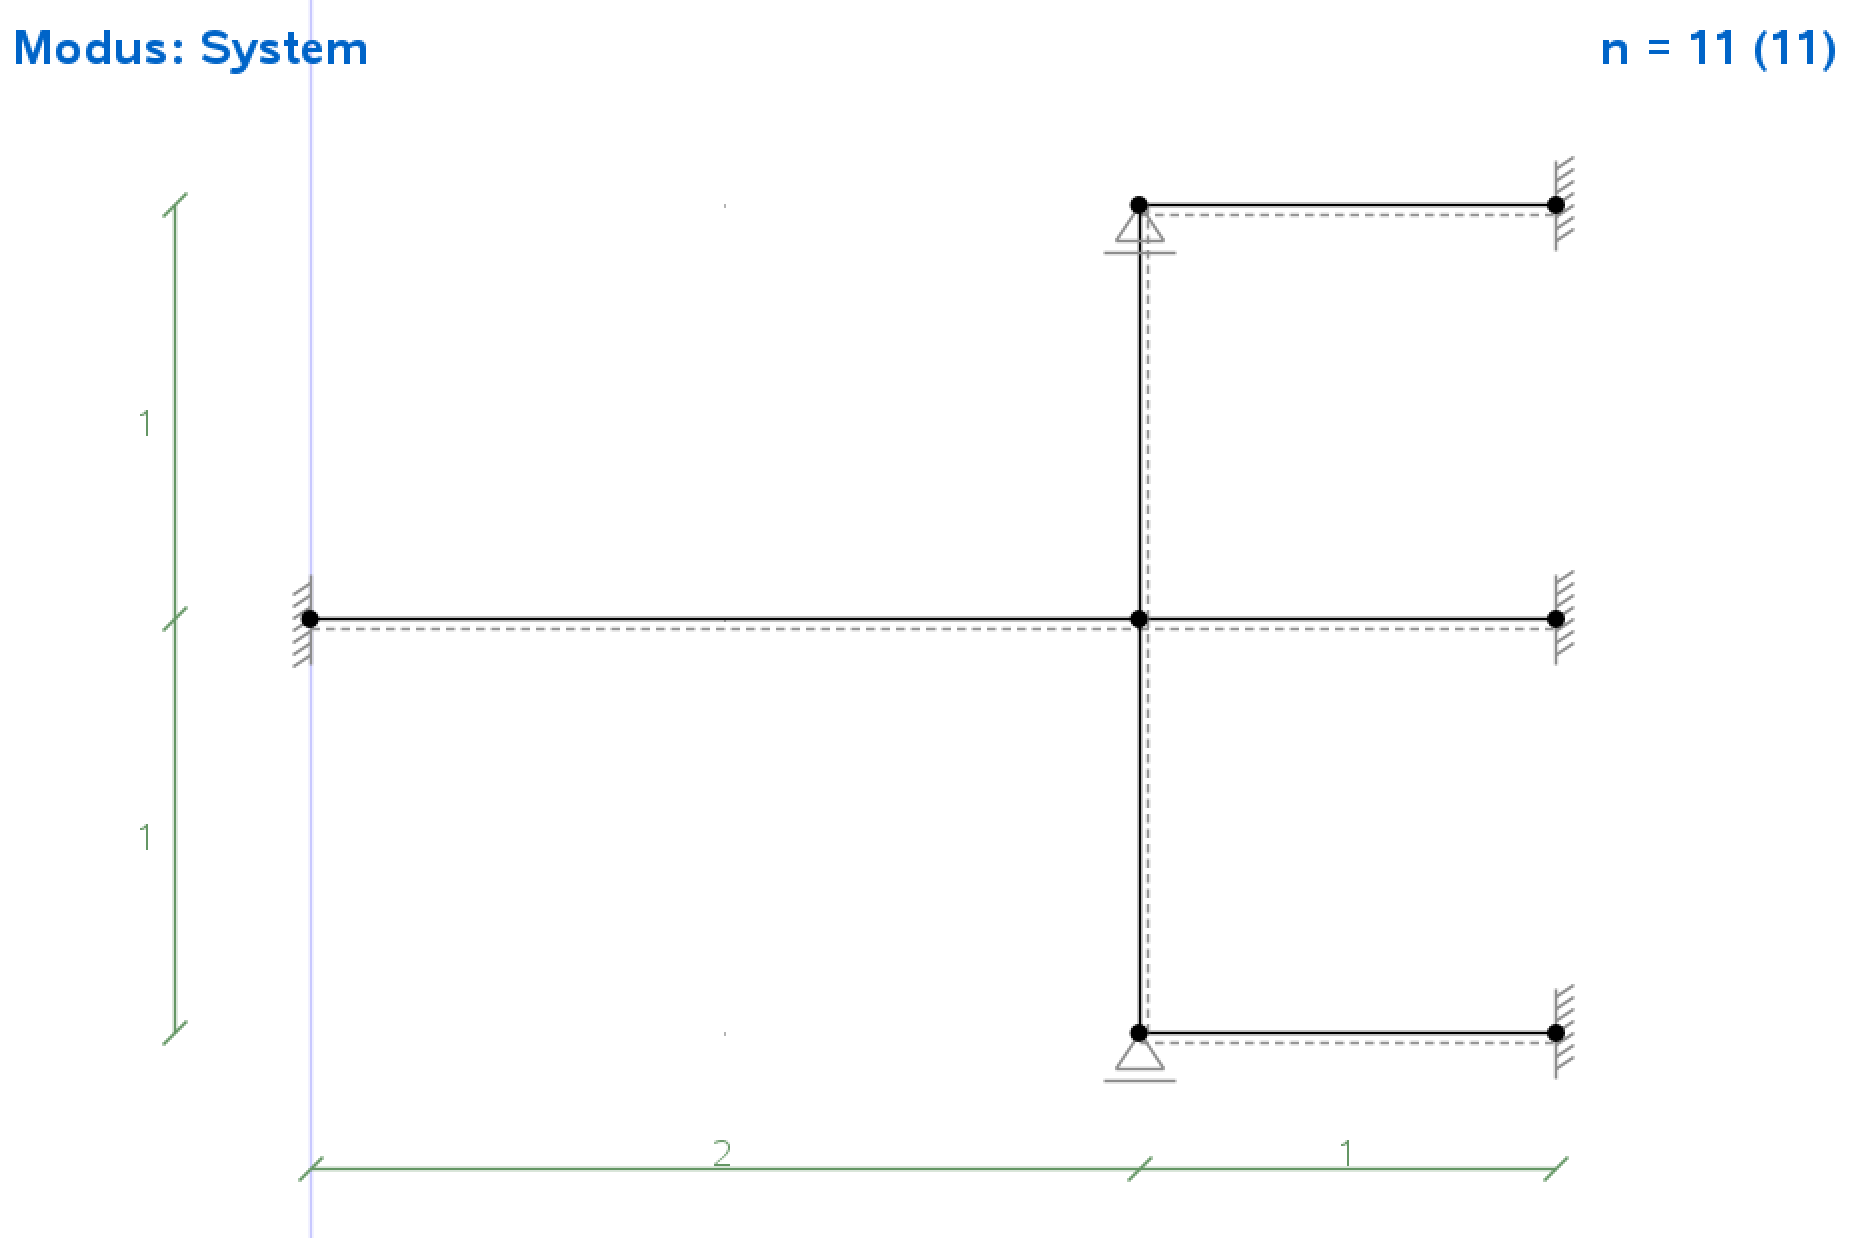
\includegraphics[width=0.5\linewidth]{./fig/TM2/WiSe2021nr4_3.png}
    \caption{TM2 WiSe~20/21, Nr.~4b im Programm}
    \label{fig:VerschiebungTemp}
\end{figure}

Da das Programm nur schnittgrößen direkt berechnet müssen diese noch in Spannungen umgerechnet werden, dafür gibt es in diesem Fall
zwei Möglichkeiten (vgl. Abb.\ref{fig:TM2WiSe2021Nr4b}). Entweder man rechnet die Spannunge direkt über die Schnittkraftverläufe aus,
oder über die Ableitung der Verschiebungsfunktion. Für die zweite Methode muss jedoch darauf geachtet werden den Temperatur Anteil
korrekt zu verrechnen.\\
Erstere Methode ist für Aufgaben mit Zahlenwerten auf jeden Fall die Einfachere, für Aufgaben mit symbolischen Temperatur Werten muss jedoch
die zweite Methode gewählt werden, da die Schnittkraftverläufe diese nicht auf die gewünschte Art berücksichtigen.

\begin{figure}[htbp]
    \centering
    \begin{subfigure}[t]{0.48\textwidth}
        \centering
        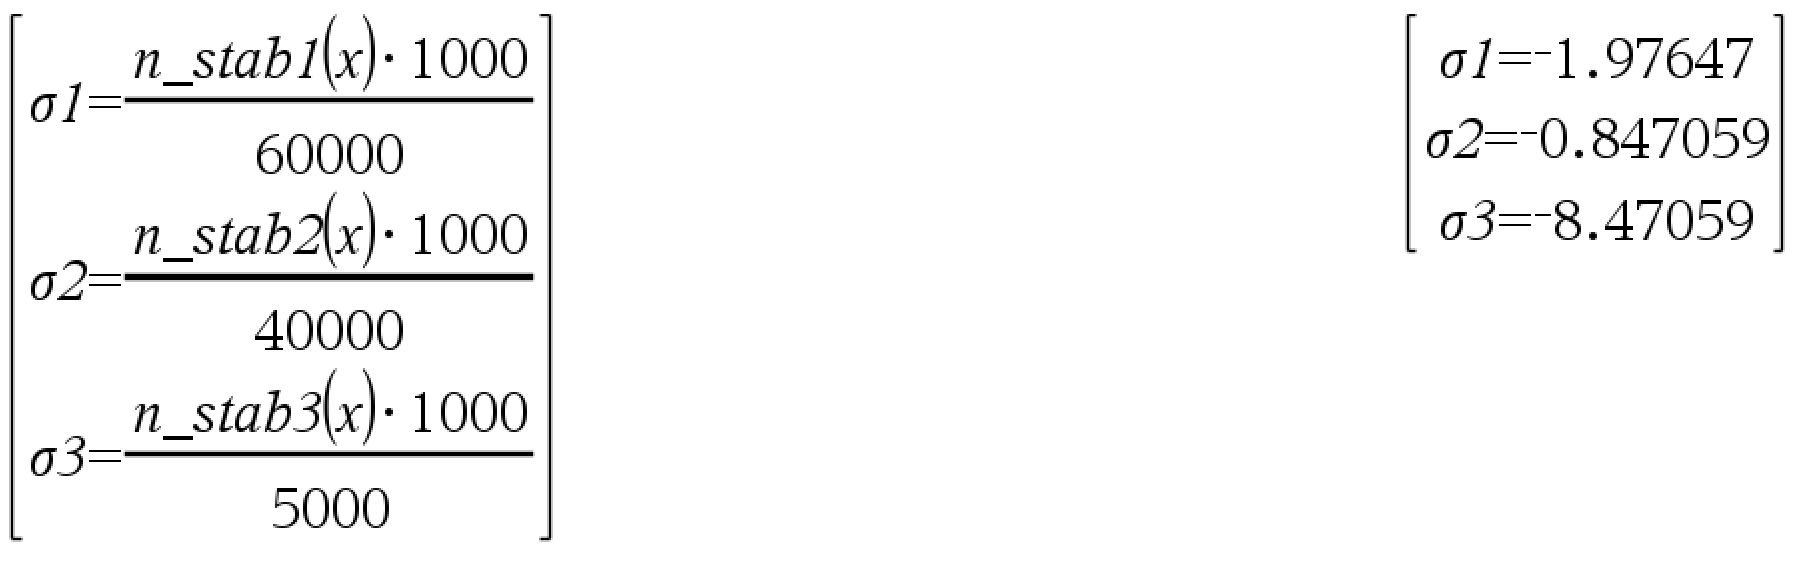
\includegraphics[width=\linewidth]{./fig/TM2/WiSe2021nr4_4.png}
        \caption{Über Schnittgrößen}
    \end{subfigure}
    \hfill
    \begin{subfigure}[t]{0.48\textwidth}
        \centering
        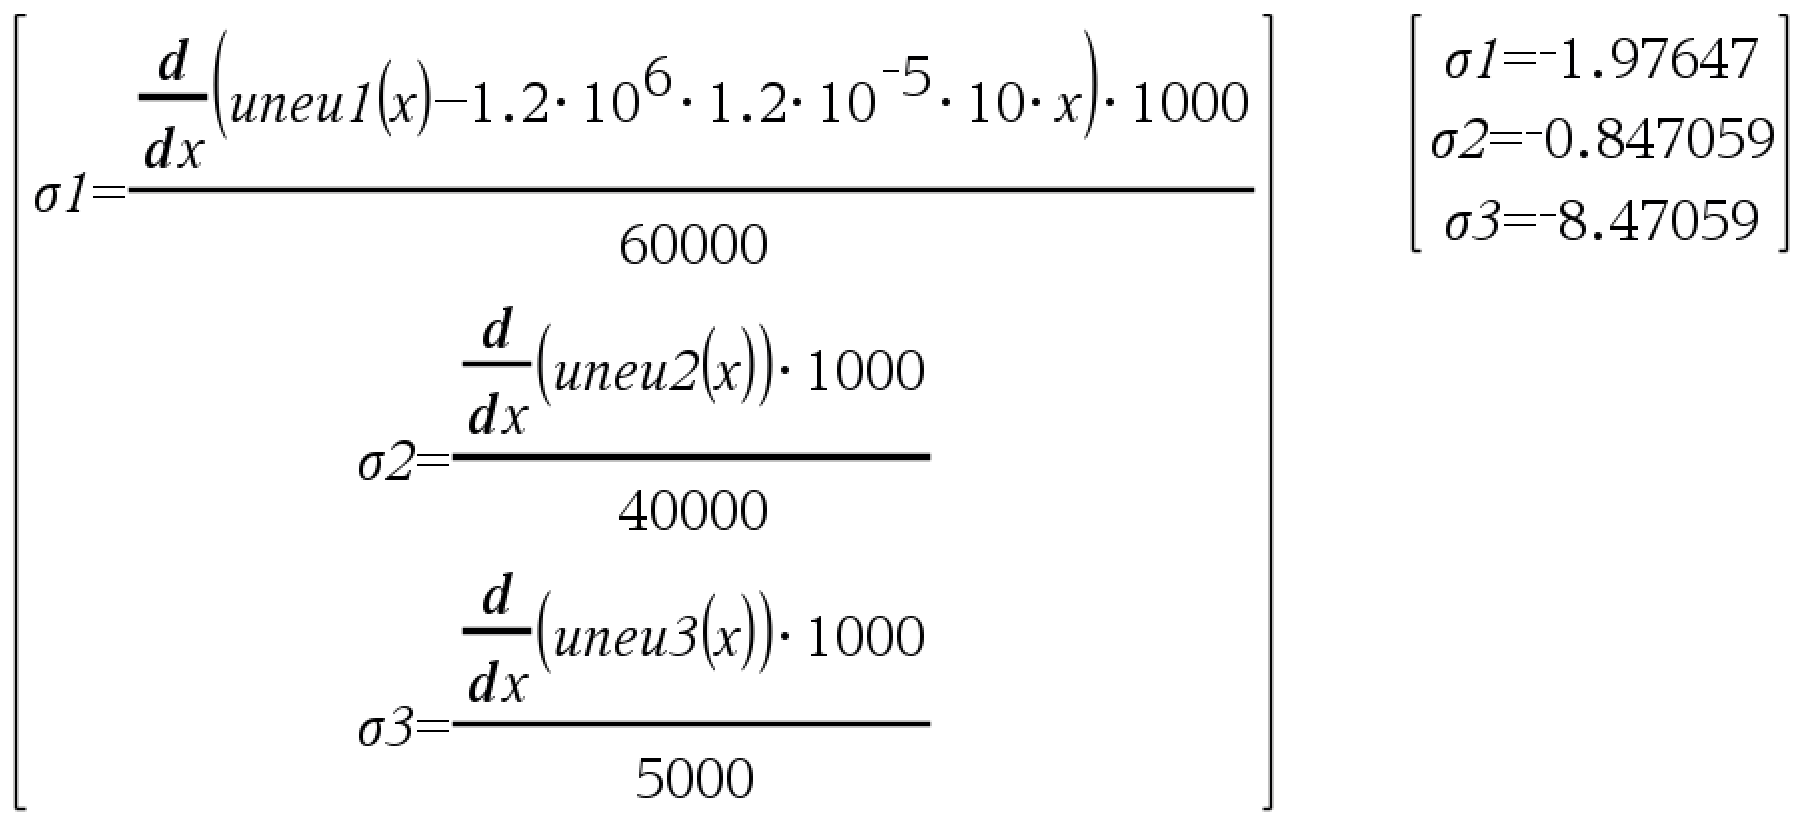
\includegraphics[width=\linewidth]{./fig/TM2/WiSe2021nr4_5.png}
        \caption{Über Verschiebungsfunktion}
    \end{subfigure}
    \caption{Lösung von TM2 WiSe~20/21, Nr.~4b}
    \label{fig:TM2WiSe2021Nr4b}
\end{figure}

Ich will hier anmerken das bei dieser Aufgabenart häufig Hinweise und Warnungen angezeigt werden. Wie z.B. hier auch bei Teilaufgabe a) eine Warnung
zur symbolischen Temperatur. Diese Warnungen sind zwar so konzipiert, dass sie nur angezeigt werden wenn das Programm bzw. ich denke
das etwas falsch eingegeben wurde, jedoch ist es schwer dabei zu vermeiden das auch bei richtiger Eingabe nie eine Warnung oder Hinweis kommt.
Aus diesem Grund empfehele ich, wenn nicht direkt ersichlich ist warum eine Warnung kommt die komplette Eingabe nochmal zu prüfen,
falls diese aber wirklicht korrekt ist sollten auch die Ergebnisse stimmen.


\subsection{Pendelstabannahme (TM2 WiSe 22/23 Nr.~4)} \label{ex:Pendelstabannahme}

\begin{figure}[htbp]
    \centering
    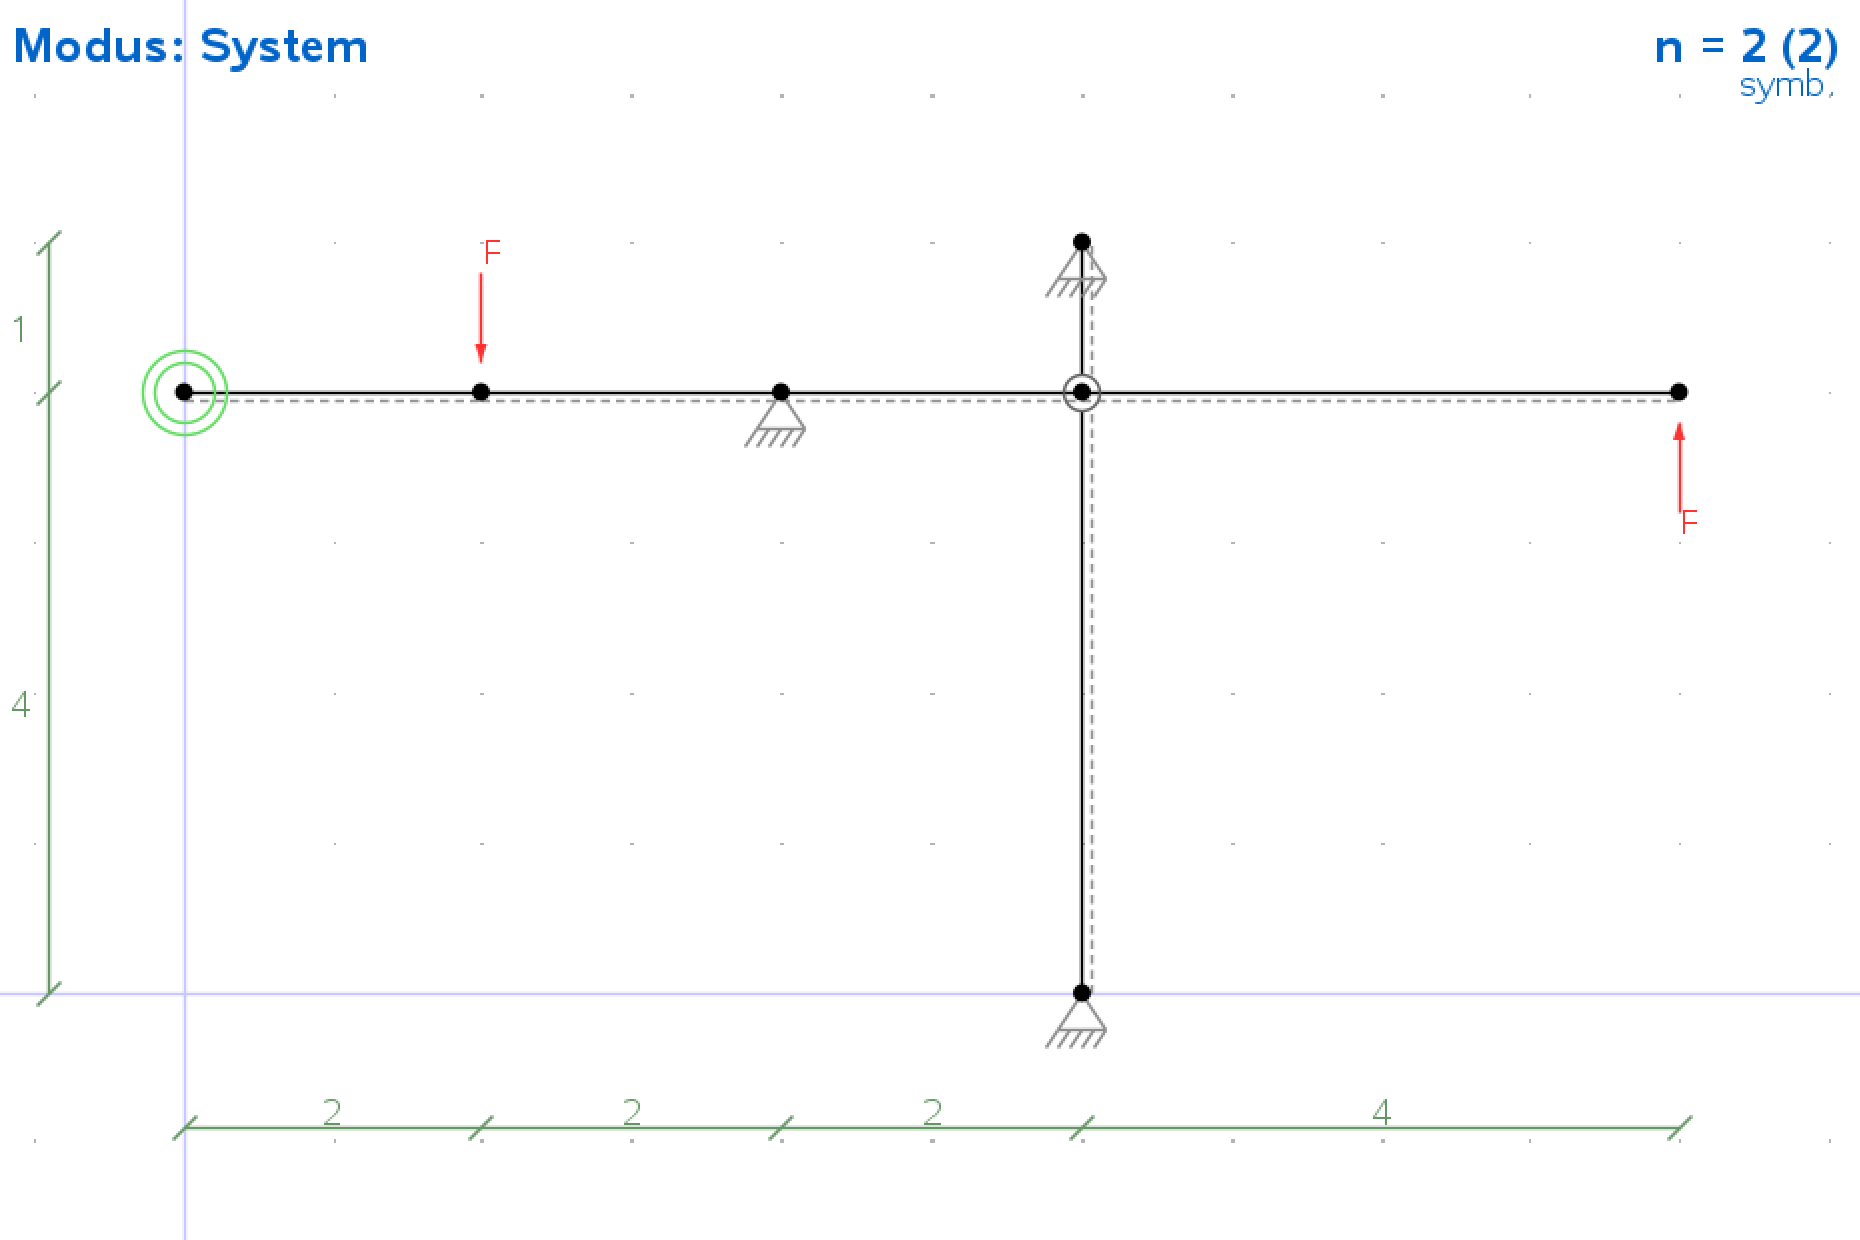
\includegraphics[width=0.7\linewidth]{./fig/TM2/WiSe2223nr4_1.png}
    \caption{TM2 WiSe~22/23, Nr.~4 im Programm}
    \label{fig:Pendelstabsnnahme}
\end{figure}

Wie die Überschrifft vielleicht bereits vermuten lässt muss bei dieser Aufgabe eine Annahme getroffen werden,
die der Zeichnung strenggenommen wiederspricht. Die beiden vertikalen stäbe sollten eigentlich mit einem Angelenk
an den starren Stab angeschlossen werden.\\
Bei einer Handrechnung wird diese Annahme quasi automatisch getroffen, das Programm macht sowas natürlich nicht automatisch.
Um diese Aufgabe mit dem Programm also korrekt zu rechnen müsseb bei den beiden vertikalen stäbe jeweils Angelenke eingebaut werden.
Falls man das nicht macht wirft das Programm eine Warnung bzw. einen Hinweis.

Bei dieser Aufgabe lassen sich die Ergebnisse entweder aus der Ansicht zur Normalkraft 
oder aus dem E-Modus holen (Abb.~\ref{fig:TM2WiSe2223Nr4}).

\begin{figure}[htbp]
    \centering
    \begin{subfigure}[t]{0.48\textwidth}
        \centering
        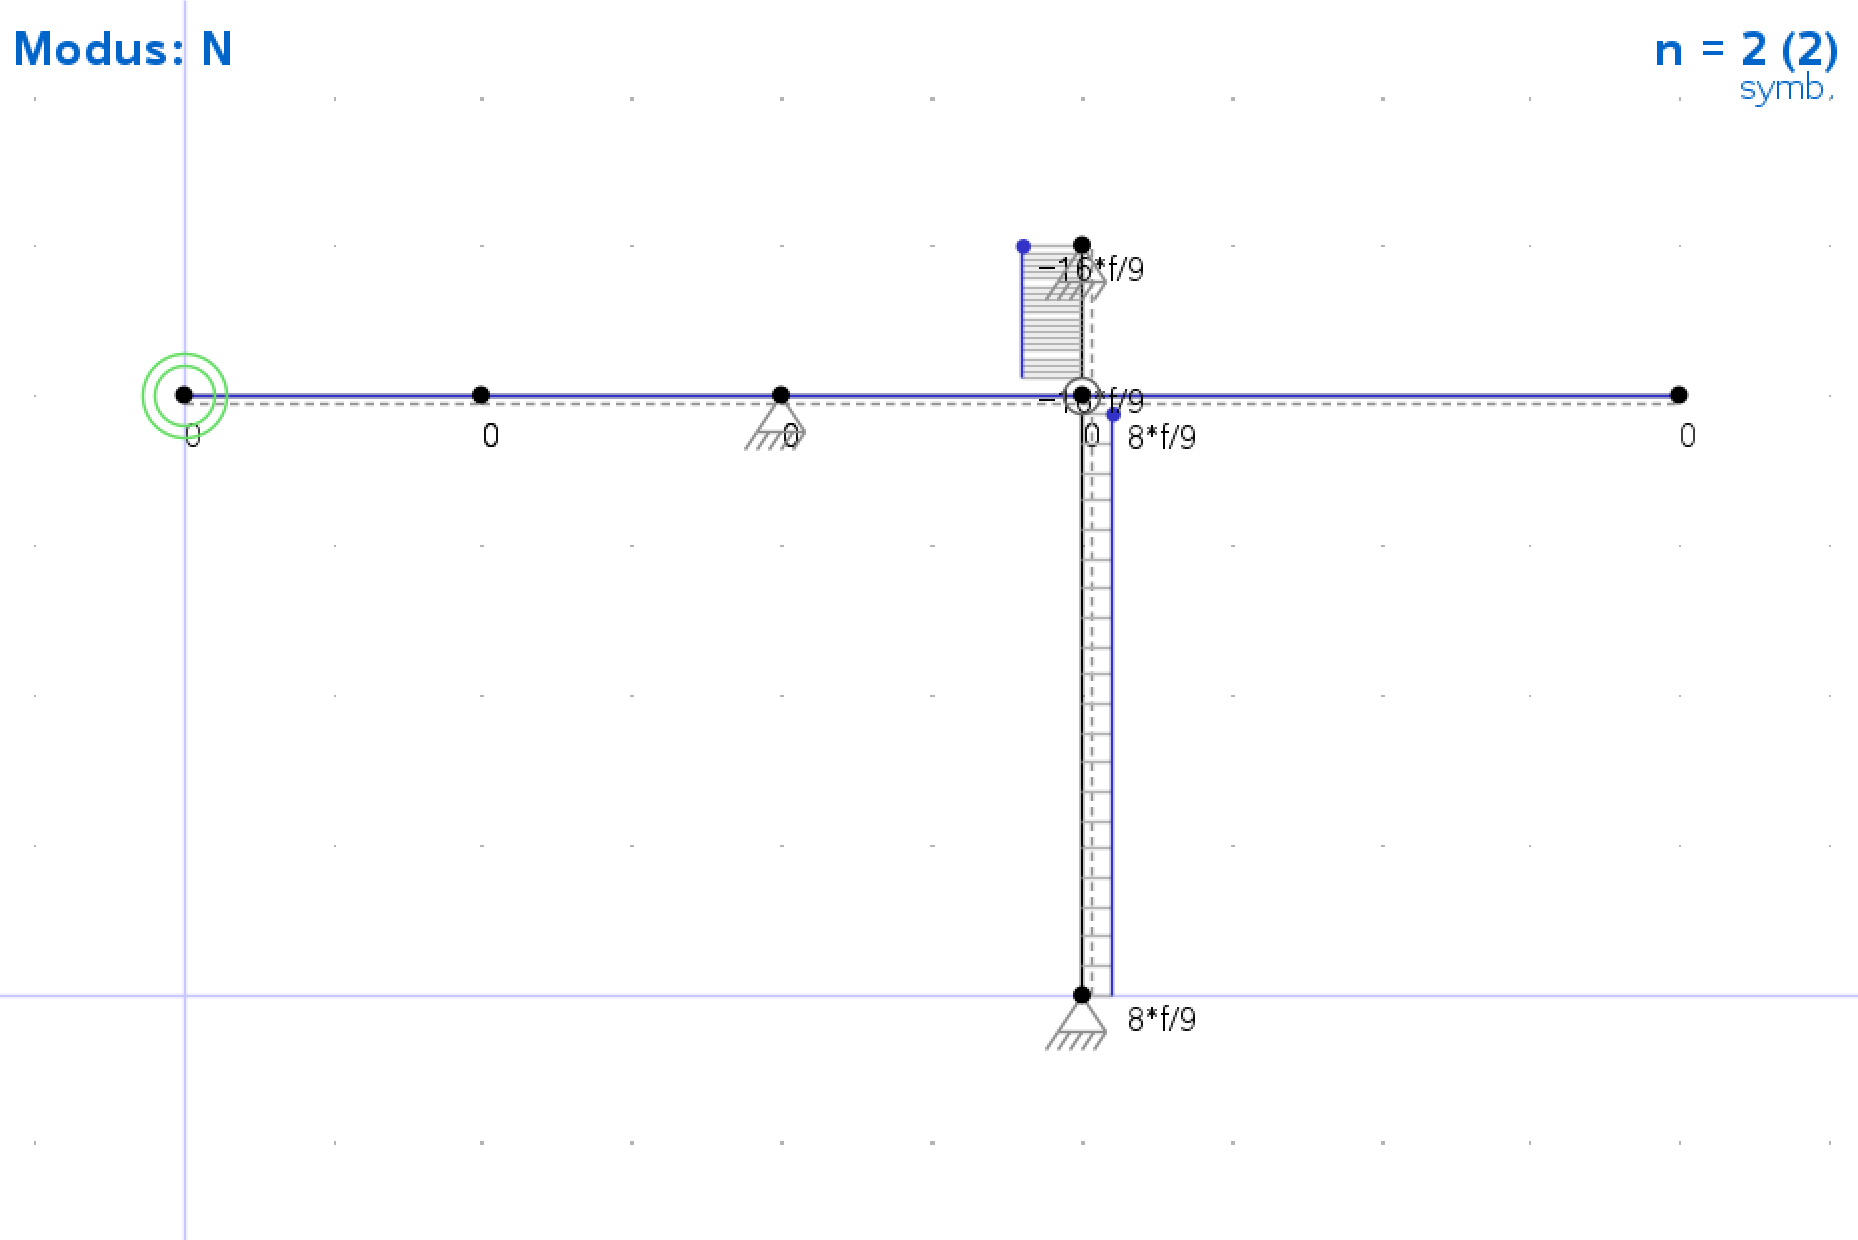
\includegraphics[width=\linewidth]{./fig/TM2/WiSe2223nr4_2.png}
        \caption{Normalkraft}
    \end{subfigure}
    \hfill
    \begin{subfigure}[t]{0.48\textwidth}
        \centering
        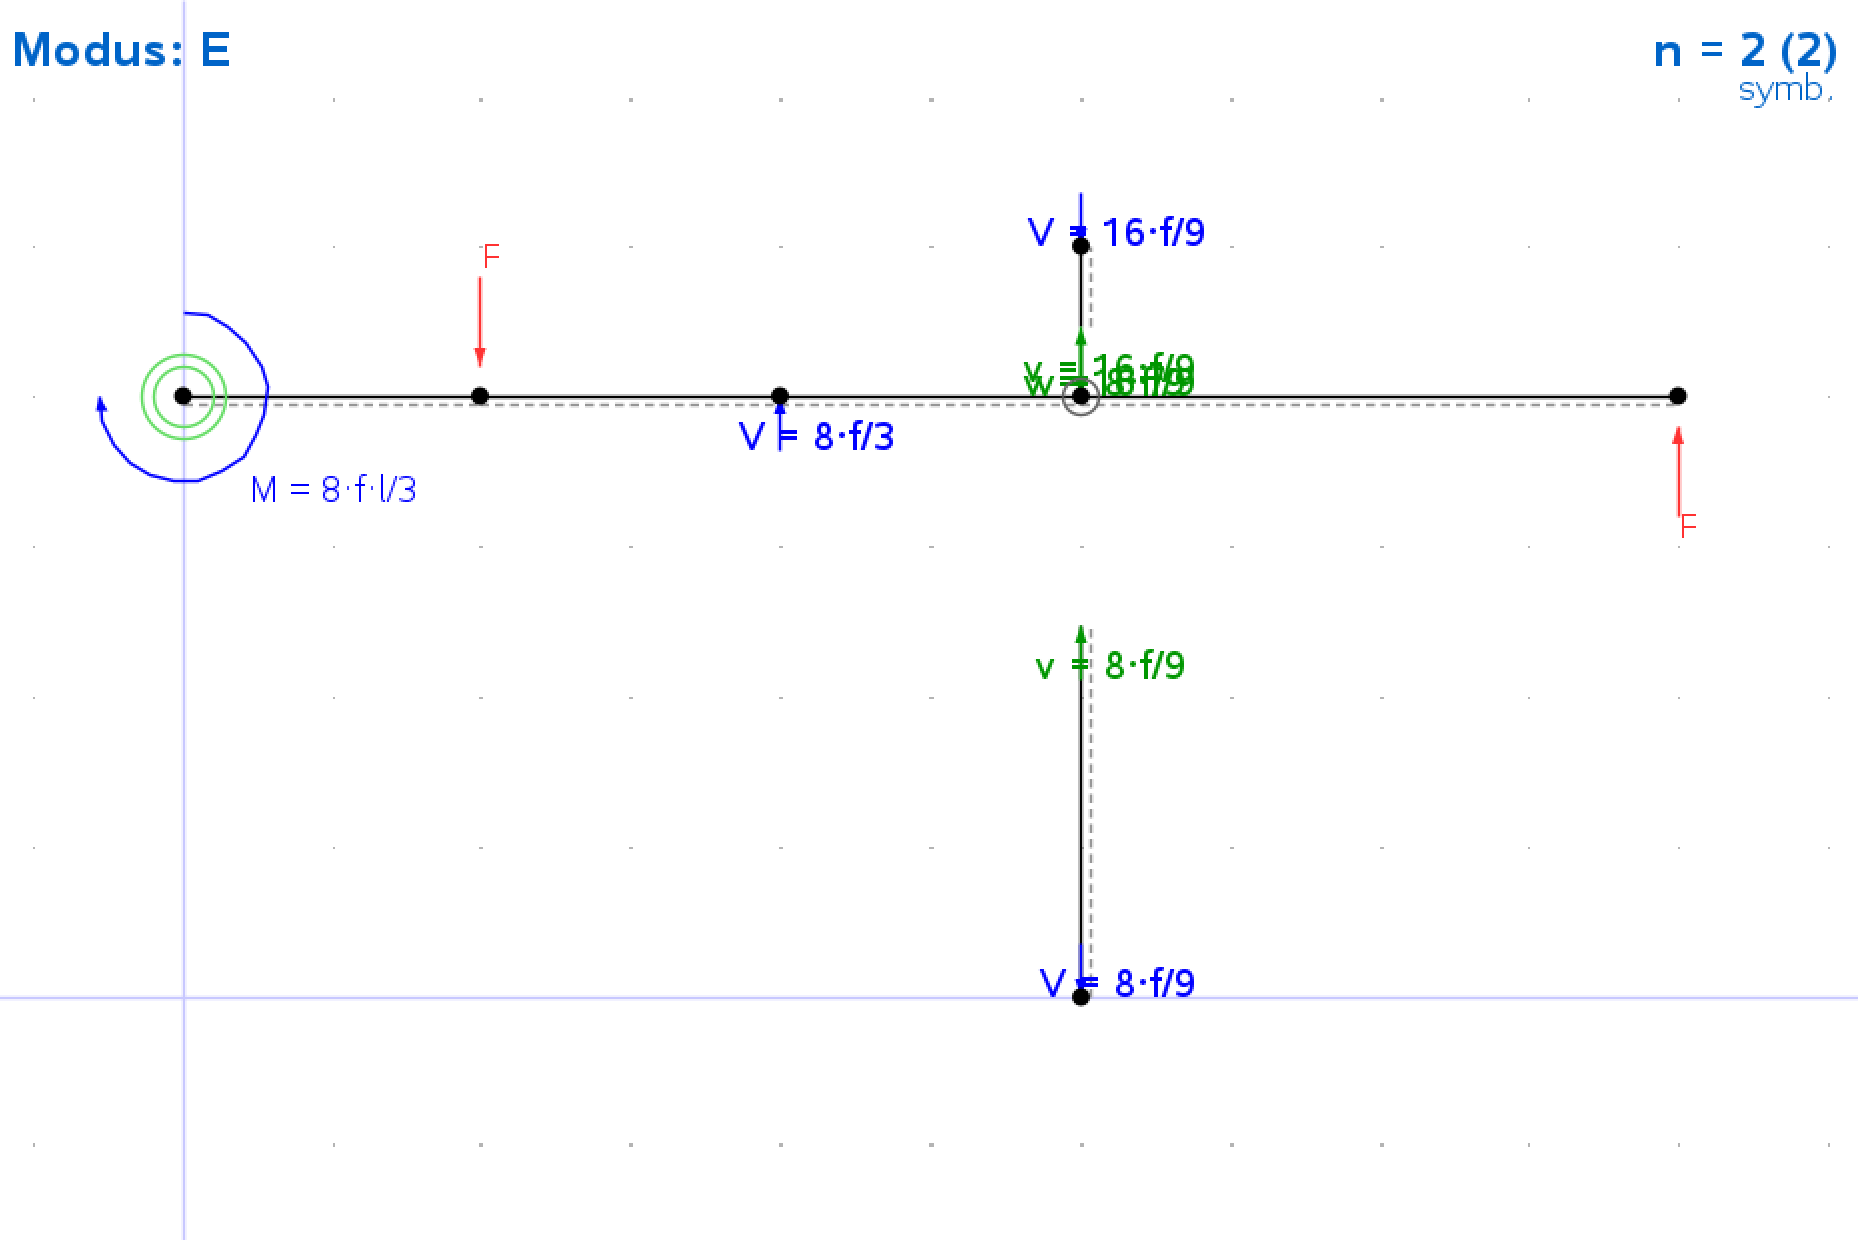
\includegraphics[width=\linewidth]{./fig/TM2/WiSe2223nr4_3.png}
        \caption{E-Modus}
    \end{subfigure}
    \caption{Lösung von TM2 WiSe~22/23, Nr.~4}
    \label{fig:TM2WiSe2223Nr4}
\end{figure}

\textbf{Wichtig} ist, dass das Programm, für symbolische Federn in den Verläufen in seltenen Fällen nicht die richtigen 
Werte ausgibt (Bei symbolischen Temperaturen sowieso nicht).
Zur Sicherheit würde ich deswegen die Schnittgrößen über die \emph{neuen} Verschiebungsfunktionen ermitteln. 
Das dauert zwar gerade für große Systeme länger, ist aber zuverlässiger weil dort wirklich alles symbolisch gerechnet wird 
und eben nicht gepfuscht wird.



\subsection{Schiefe Biegung (TM2 WiSe 25/26 Nr.~8)}

In dieser Aufgbabe sind die Dicken der dünnwandigen Elemente nicht gegeben, da diese abber sowohl für das
FTM als auch für die Lange des Schwerpunkts wichtig sind, müssen diese Werte manuell mit den Werten aus der 
Aufgabenstellung überschrieben werden. Das geht im Obermenue (Taste \taste{o}) auf Seite 3.\\
Für das Zeichnen so eines schiefen Querschnitts empfielt sich ein Rastermaß von z.B. $\frac{1}{\sqrt{2}}$.

\begin{figure}[htbp]
    \centering
    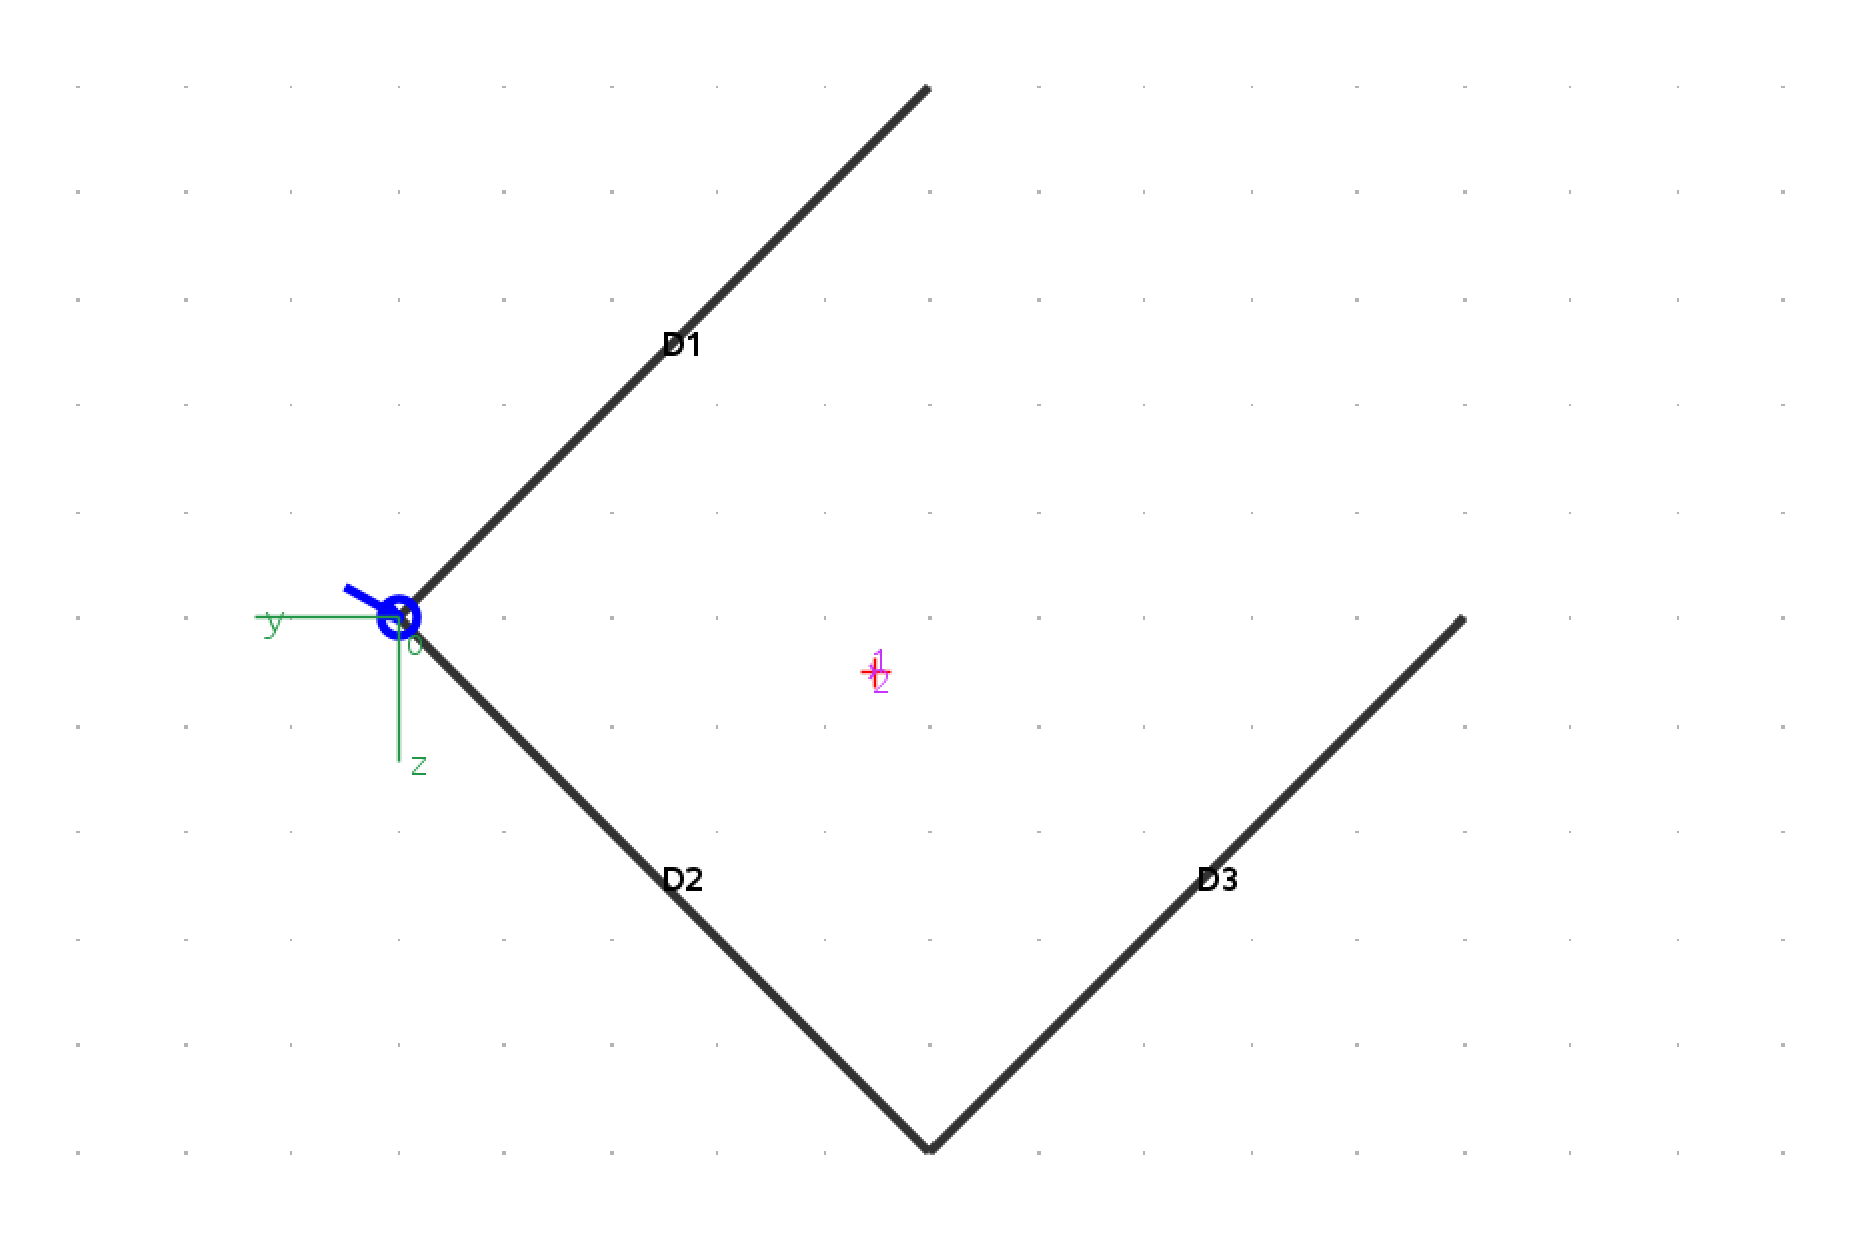
\includegraphics[width=0.7\linewidth]{./fig/TM2/WiSe2526nr8_1.png}
    \caption{TM2 WiSe~25/26, Nr.~8 im Programm}
    \label{fig:TM2WiSe2526Nr8_1}
\end{figure}

Bei dieser Aufgabe braucht man die $\sigma_x$-Berechnung. Um die Normalkraft hier richtig einzuberechnen
muss die Resultierende der Streckenlast über die halbe Länge berechnet werden, also: 
$R=0,1~\frac{\text{kN}}{cm}\cdot100~\text{cm}$.
Für die Kraft muss also $F_y=-500~\text{N}$, $F_z=300~\text{N}$ und $F_x=10000~\text{N}$ eingegeben werden.

Nach dem Aufruf der Berechnung werden noch ein paar Werte abgefragt. Für die ersten Drei muss Null eingetragen werden.
Man hätte auch keine Kraft platzieren können, die Normalkraft und Momente handisch ausrechnen können und diese dann in diese Felder eintragen können.
Das Ergebniss ist das gleiche.\\
Für $\Delta x$ muss $100~\text{cm}$ eingetragen werden, das ist der Abstand zwischen dem gezeichneten Schnitt und dem betrachteten Schnitt.
Das Programm rechnet dann also automatisch die Momente aus der Querkraft aus. Dieses Feature funktioniert natürlich nur, wenn zwischen dem gezeichneten und berechneten Schnitt
keine Weiteren Einflüsse wie Lager oder Kräfte Angreiffen, dann kommt man nicht darum herum $N$, $M_y$ und $M_z$ händisch auszurechnen und einzutragen.

Die Ergebnisse sind in Abbildung \ref{fig:TM2WiSe2526Nr8_2} dargestellt.

\begin{figure}[htbp]
    \centering
    \begin{subfigure}[t]{0.48\textwidth}
        \centering
        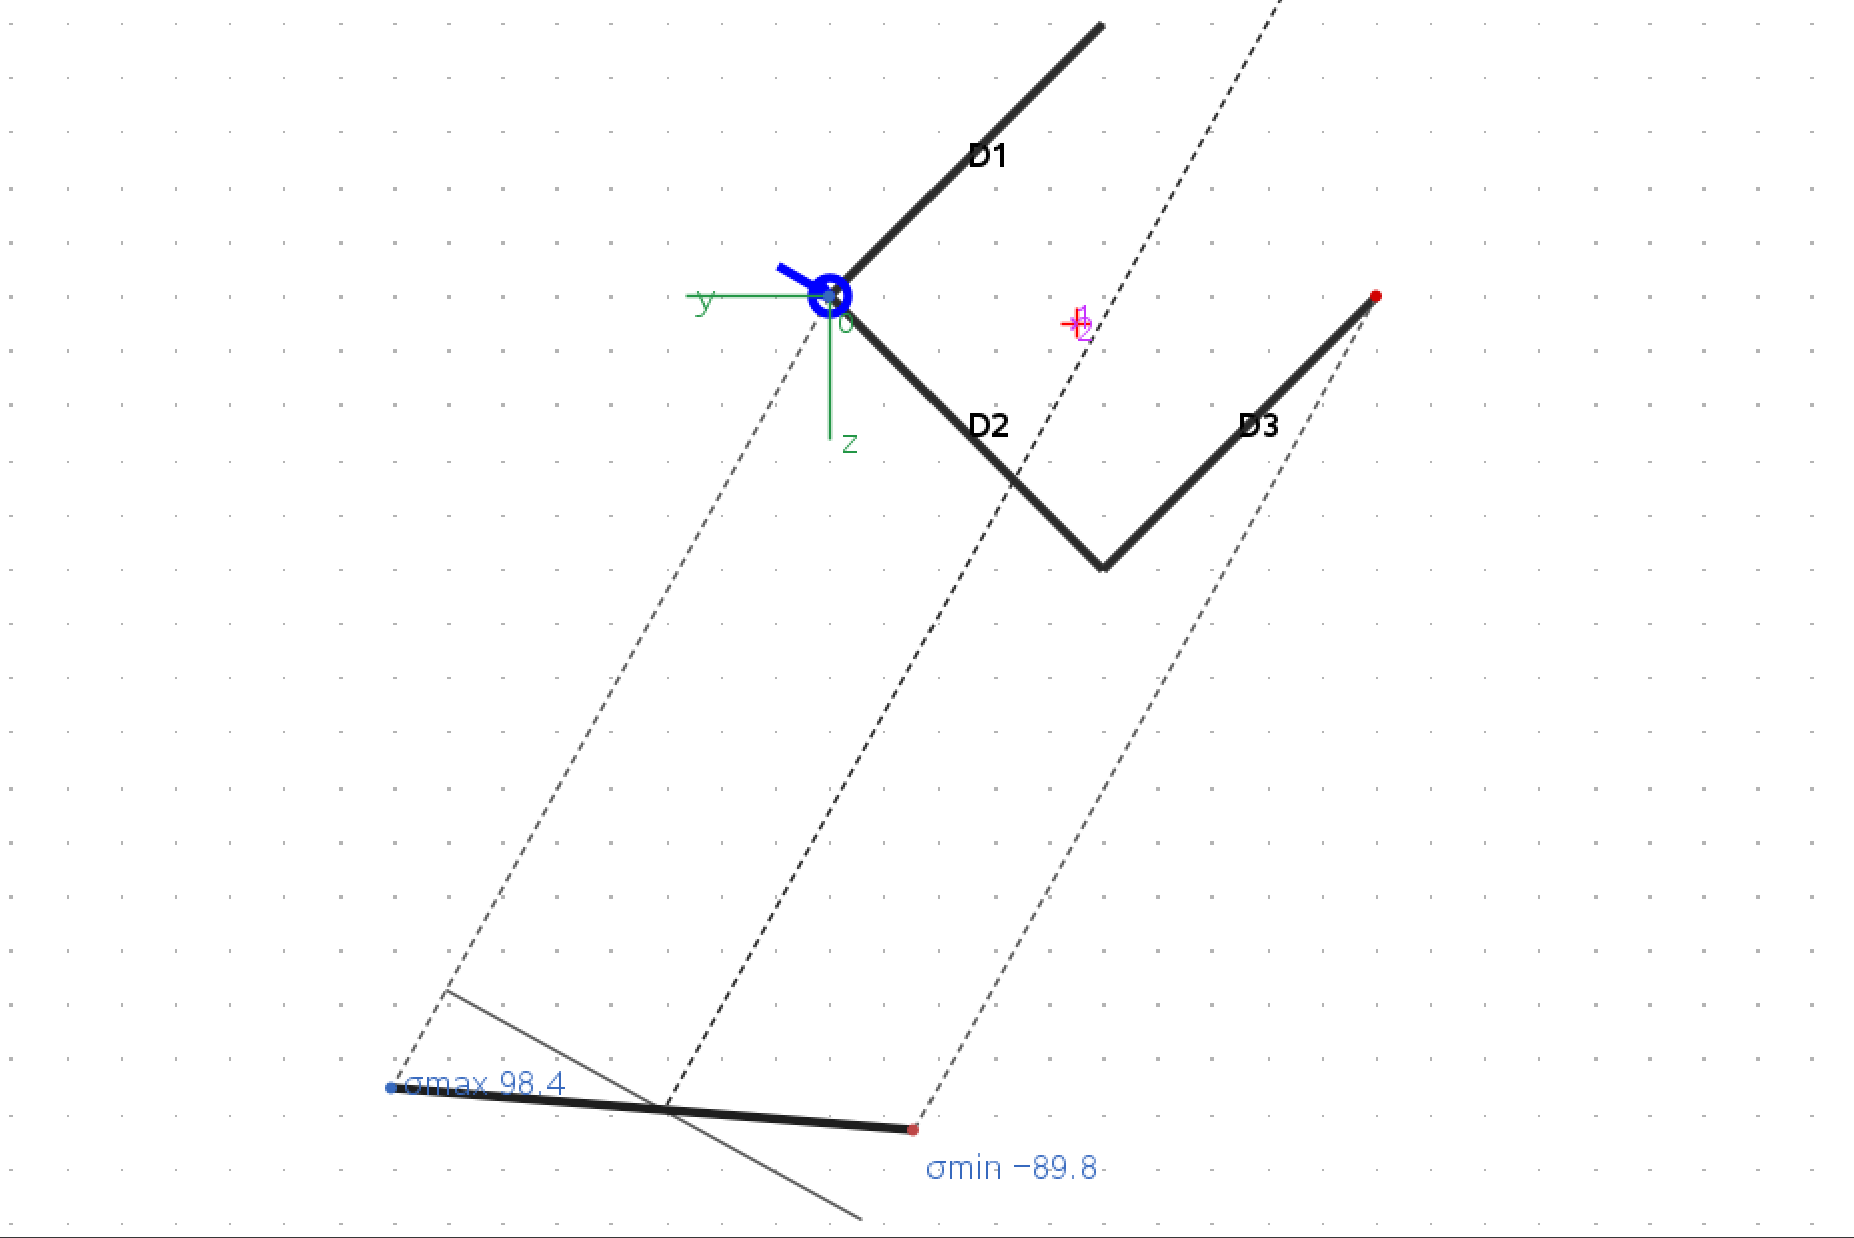
\includegraphics[width=\linewidth]{./fig/TM2/WiSe2526nr8_2.png}
        \caption{Spannungsverlauf}
    \end{subfigure}
    \hfill
    \begin{subfigure}[t]{0.48\textwidth}
        \centering
        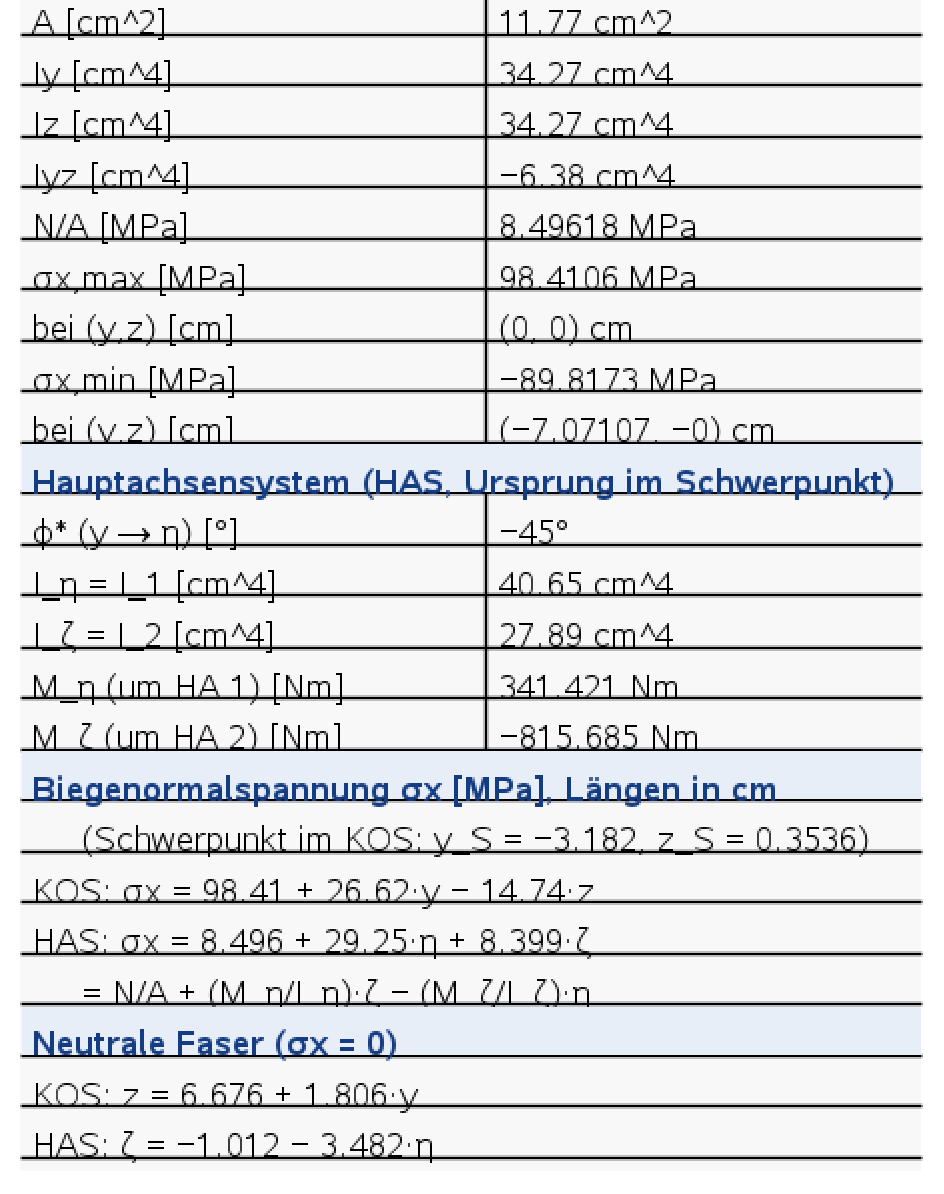
\includegraphics[width=\linewidth]{./fig/TM2/WiSe2526nr8_3.png}
        \caption{Tabellen übersicht}
    \end{subfigure}
    \caption{Lösung von TM2 WiSe~25/26, Nr.~8}
    \label{fig:TM2WiSe2526Nr8_2}
\end{figure}

Ich will anmereken, dass des öfteren bei Aufgaben Querschnittswerte gegeben sind, die nicht zur Bemaßung in der Zeichnung passen,
ob das absichtlich so ist konnte mir leider keiner sagen. Es ist also immer sinnvoll das einmal gegen zu prüfen und die Werte evtl. zu überschreiben.
Was die ISD-Musterlösung bei dieser Aufgabe gerechnet hat, ist mir nicht ganz klar. Meines Verständnisses nach wurde hier mit einem
Schwerpunkt für die Momente aus Normalkraft gerechnet, der genau in der Mitte des U profiels liegt, sodass die Normalkraft um die $y$-Achse kein Moment erzeugt.

\subsection{Schiefe Biegung/Kernfäche (TM2 WiSe21/22 Nr.~8)}



\subsection{MSK (TM2 WiSe 21/22 Nr.~3)}

Zu dieser Aufgabe gibt es eigentlich nicht besonders viel zu sagen, man gibt die gegebenen Werte ein und das Programm
füllt in grün die restlichen Werte auf (Abb.~\ref{fig:TM2WiSe2122Nr3_1}).

\begin{figure}[htbp]
    \centering
    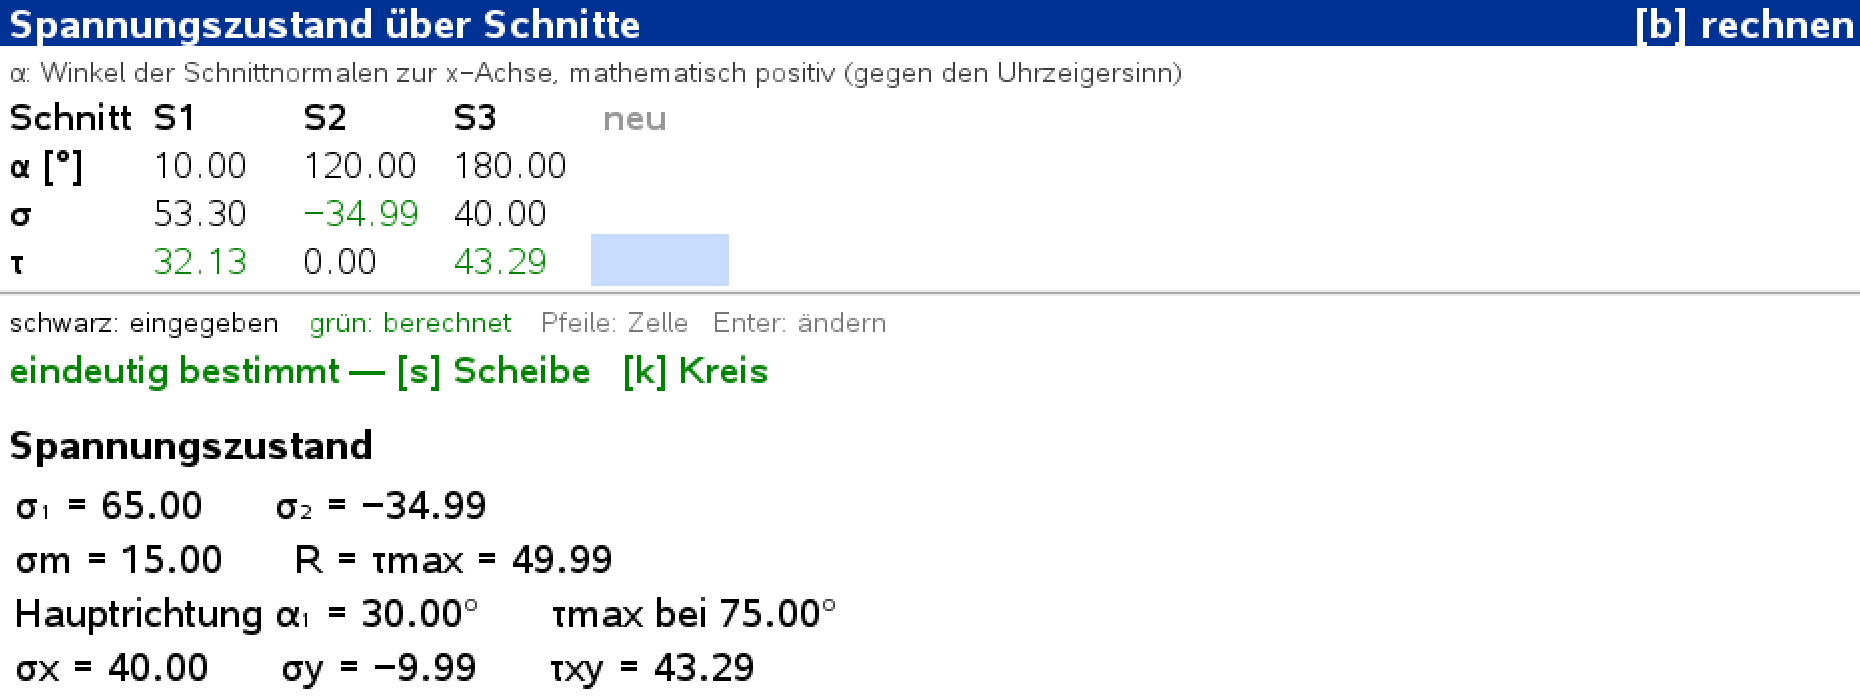
\includegraphics[width=0.7\linewidth]{./fig/TM2/WiSe2122nr3_1.png}
    \caption{TM2 WiSe~21/22, Nr.~3 im Programm}
    \label{fig:TM2WiSe2122Nr3_1}
\end{figure}

Danach bekommt man mit den Tasten \taste{s} und \taste{k} die beiden wichtigen Ansichten (Abb.~\ref{fig:TM2WiSe2122Nr3_2}).


\begin{figure}[htbp]
    \centering
    \begin{subfigure}[t]{0.48\textwidth}
        \centering
        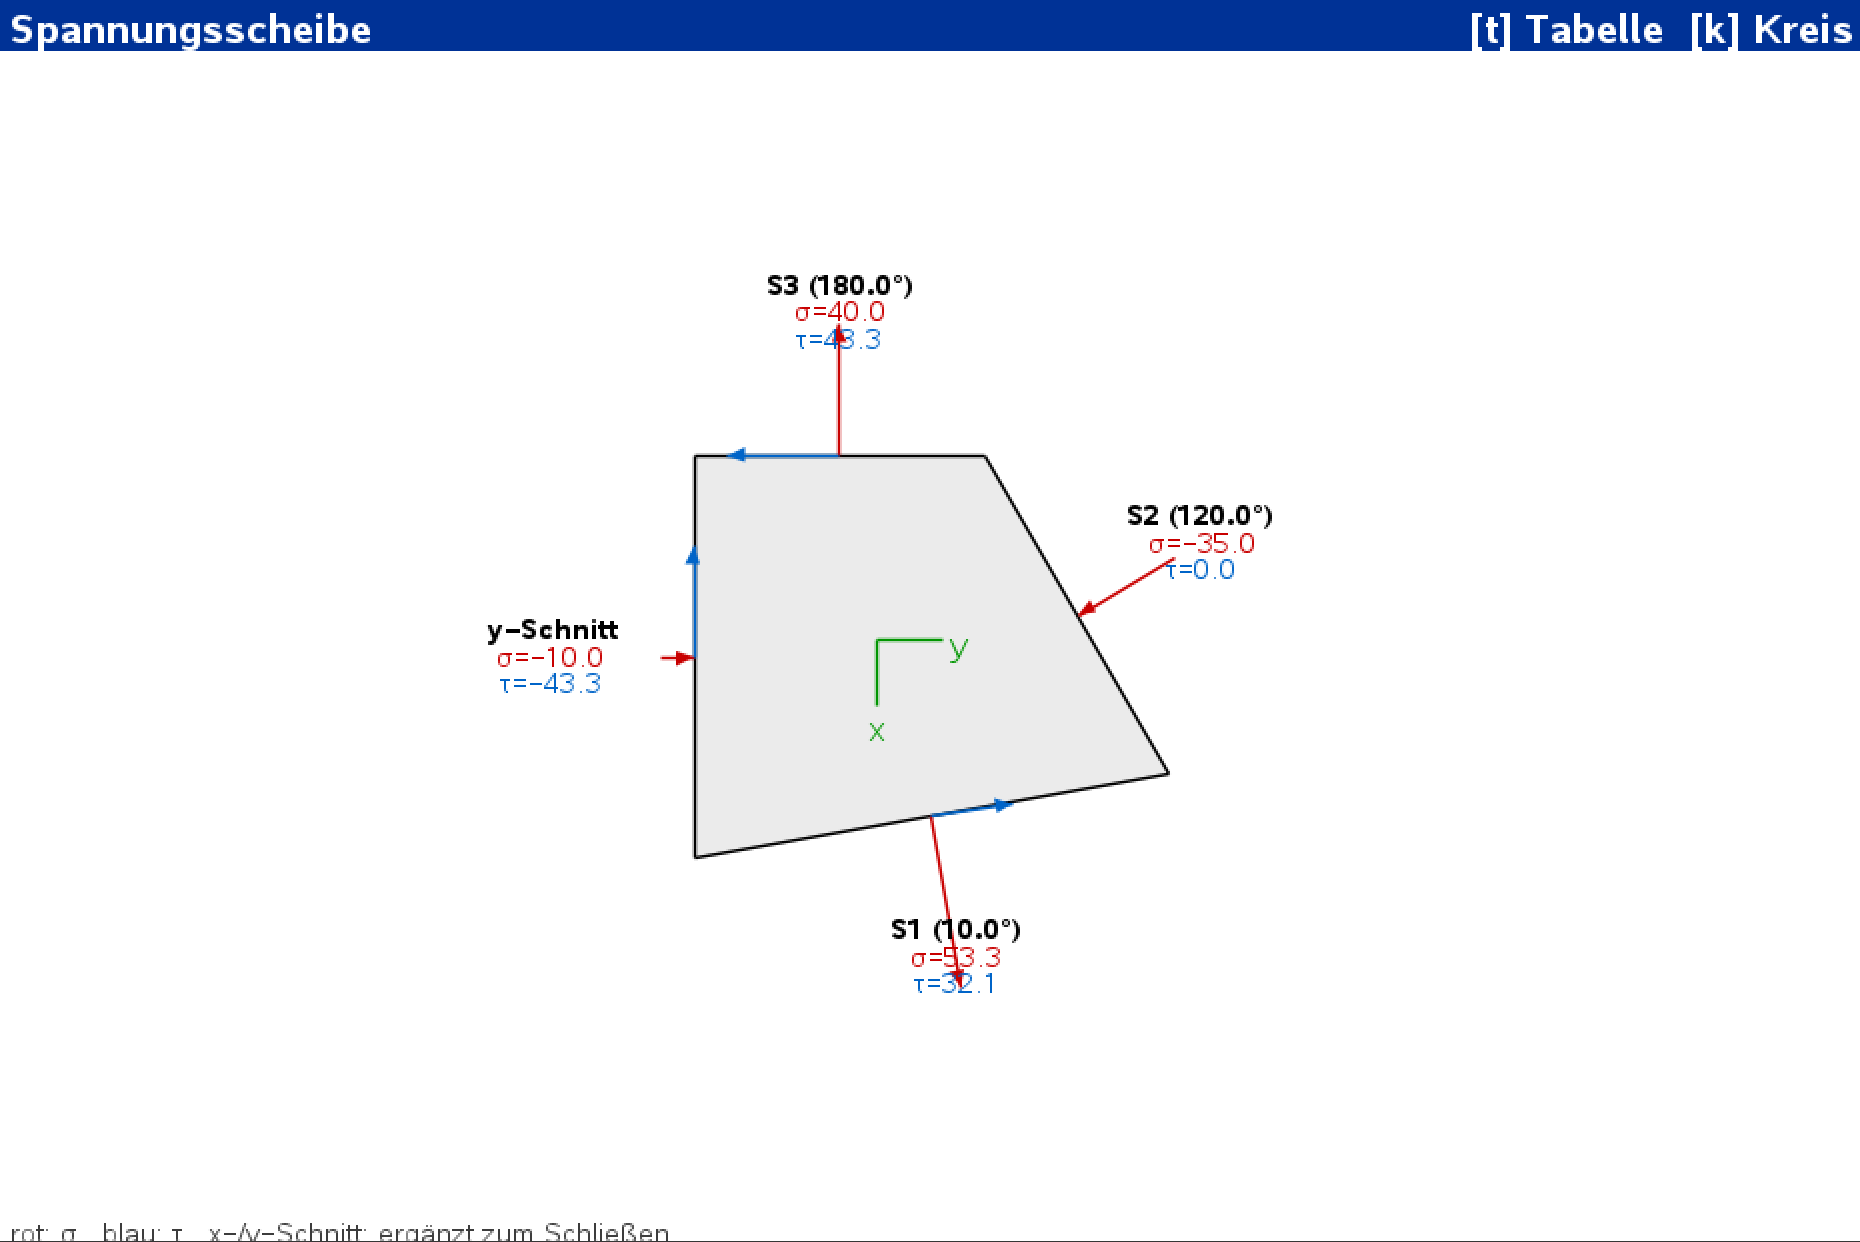
\includegraphics[width=\linewidth]{./fig/TM2/WiSe2122nr3_2.png}
        \caption{Spannungs-Scheibe}
    \end{subfigure}
    \hfill
    \begin{subfigure}[t]{0.48\textwidth}
        \centering
        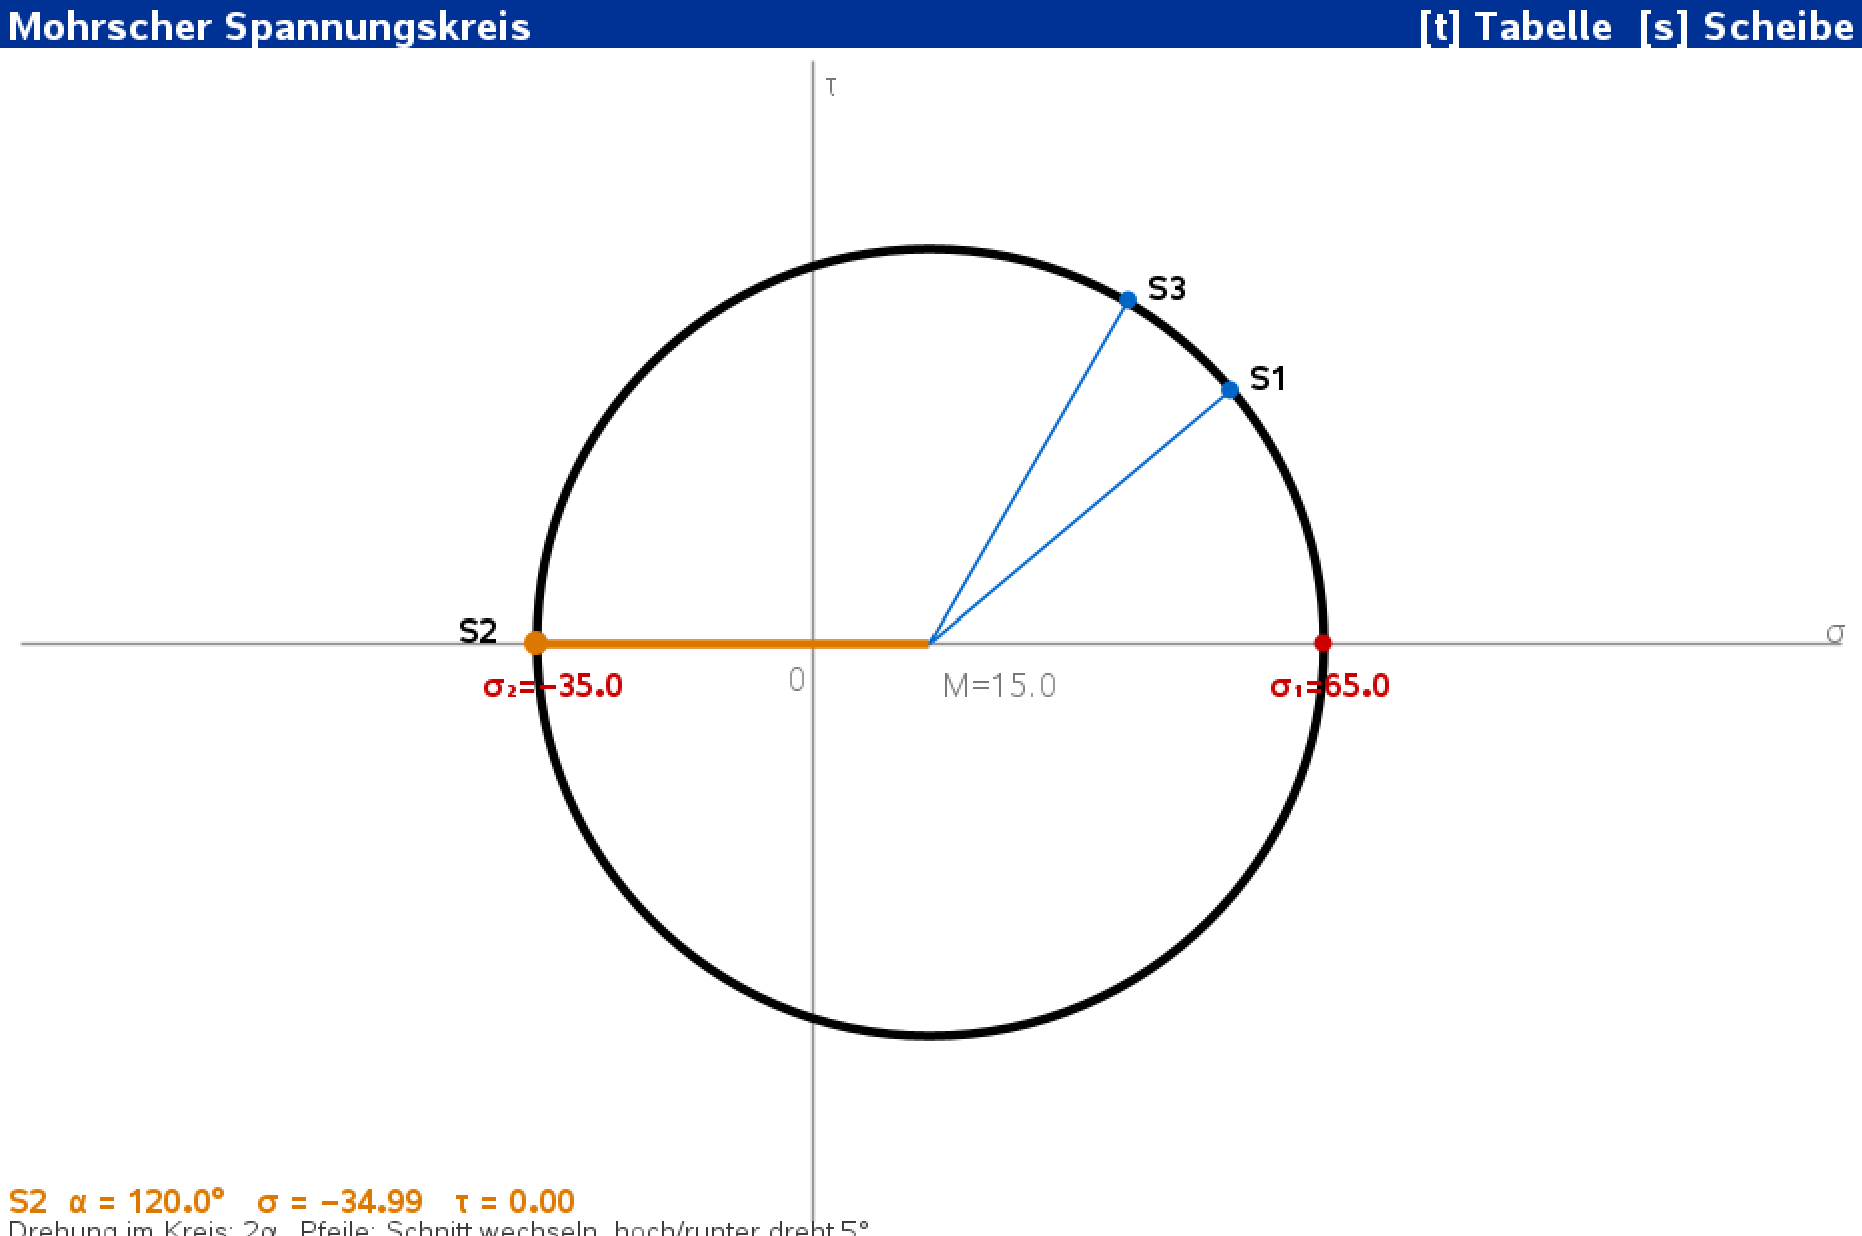
\includegraphics[width=\linewidth]{./fig/TM2/WiSe2122nr3_3.png}
        \caption{Spannungs-Kreis}
    \end{subfigure}
    \caption{Lösung von TM2 WiSe~21/22, Nr.~3}
    \label{fig:TM2WiSe2122Nr3_2}
\end{figure}

Falls bei einer Aufgabe nach dem Winkel eines Schnitts gefragt wird und das Programm zwei Winkel ausgibt, muss natürlich
geprüft werden, welcher Winkel eher zur Skizze passt.

\subsection{Schubspannung und SMP (TM2 SoSe 24 Nr.~8)}

\subsection{Verwölbung (TM2 SoSe 20 Nr.~9)}